\documentclass[12pt, twoside]{report}
\PassOptionsToPackage{x11names,usenames,dvipsnames}{xcolor}
%Font Family
%\usepackage{mathptmx}
%\usepackage[utf8]{inputenc}
%\usepackage[OT1]{fontenc}
\usepackage{helvet}		% Helvetica
%\renewcommand{\familydefault}{\sfdefault}		% Arial
%\usepackage{times}		% Times New Roman
%\usepackage{ebgaramond}	% Garamond
%\usepackage{palatino}	% Palatino
%\usepackage{charter}	% Charter
%\linespread{1.1}
%\usepackage{microtype}
\usepackage{pdfpages}

\usepackage{longtable}
\usepackage{tikz}
\usetikzlibrary{arrows.meta}
\tikzset{
  patchlbl/.style={font=\scriptsize\sffamily, text=white, inner sep=1pt},
  leader/.style  ={->,>=Latex,line width=.35pt},
  dim/.style     ={{Latex[length=3pt]}-{Latex[length=3pt]}, line width=.35pt, black},
  wit/.style     ={line width=.3pt, black!55},
  dimlbl/.style  ={font=\scriptsize, fill=white, inner sep=1pt},
}
%Numbered subsubsections
\setcounter{secnumdepth}{3} % default value for 'report' class is "2"
%Idioma español
\usepackage[spanish, es-tabla]{babel}
%Controlar donde poner imágenes y tablas
\usepackage{float}
\usepackage{natbib}
%Control sobre tabla
\usepackage{booktabs}
\usepackage{multicol}
\usepackage{multirow}
\usepackage{parskip}
\setlength{\parskip}{0.2cm plus3mm minus2mm}
\usepackage{adjustbox}
\usepackage{appendix}
\usepackage{enumerate}
\usepackage{enumitem}
\usepackage{array}
\usepackage{amsmath}
\setcounter{MaxMatrixCols}{12}
\usepackage{amsfonts}
\usepackage{enumitem}

%Símbolo para cancelar términos en ecuaciones
\usepackage{cancel}

\usepackage{minitoc}
\dominitoc          % activa minitoc globalmente
\setcounter{tocdepth}{3} % para incluir subsubsecciones

\usepackage{caption}
\usepackage{subcaption}

\usepackage{placeins,etoolbox}
\preto{\subsection}{\FloatBarrier}      % barrera antes de cada subsección
\preto{\subsubsection}{\FloatBarrier}   % barrera antes de cada subsubsección


\usepackage[utf8]{inputenc}
\usepackage{graphicx}
\graphicspath{ {images/} }
\usepackage[a4paper,width=170mm,top=20mm,bottom=20mm, bindingoffset=10mm]{geometry}

%Crear hipervínculos
\usepackage[x11names,usenames,dvipsnames]{xcolor}
\usepackage{hyperref}
\hypersetup{
    colorlinks=true,
    linkcolor=blue,
    filecolor=magenta,      
    urlcolor=cyan,
    pdftitle={Tesis de Doctorado Sebastián Oyuela}%,
%     pdfpagemode=FullScreen,
    }
\urlstyle{same}

%ECUACIONES LINDAS
\usepackage{empheq}
\definecolor{alizarin}{rgb}{0.3, 0.2, 0.5}

%CAJAS COLORIDAS
\usepackage{tcolorbox}

%Numerar ecuaciones por seccion
\numberwithin{equation}{section}
%Numerar figuras y tablas por seccion
\usepackage{chngcntr}
\counterwithin{figure}{section}
\counterwithin{table}{section}

%TITULOS DE PARRAFOS
\newcommand{\myparagraph}[1]{\paragraph{#1}\mbox{}\vspace{2mm}\\}

%TABLAS LINDAS
\usepackage{tabularx}
\usepackage{colortbl}
\tcbuselibrary{skins}
\newcolumntype{Y}{>{\raggedleft\arraybackslash}X}
\tcbset{tab1/.style={fonttitle=\bfseries\large,fontupper=\normalsize\sffamily,
colback=yellow!10!white,colframe=red!75!black,colbacktitle=Salmon!40!white,
coltitle=black,center title,freelance,frame code={
\foreach \n in {north east,north west,south east,south west}
{\path [fill=red!75!black] (interior.\n) circle (3mm); };},}}
\tcbset{tab2/.style={enhanced,fonttitle=\bfseries,fontupper=\normalsize\sffamily,
colback=yellow!10!white,colframe=red!50!black,colbacktitle=Salmon!40!white,
coltitle=black,center title}}

\usepackage{booktabs}
\usepackage{makecell}

\usepackage{tikz}
\usetikzlibrary{arrows}
\tikzset{>=latex}
\usetikzlibrary{fit, positioning}
\usetikzlibrary{babel}
\usetikzlibrary{tikzmark,decorations.pathreplacing}

\usepackage{mathtools}
\usetikzlibrary{arrows.meta}  % reemplaza old-arrows
\newcommand{\eqstackrel}[1]{\stackrel{\substack{\mathclap{#1}\\[0.5ex]\displaystyle\uparrow\\ ~}}{ = } }

\newcommand\vertarrowbox[3][6ex]{%
  \begin{array}[t]{@{}c@{}} #2 \\
  \left\downarrow\vcenter{\hrule height #1}\right.\kern-\nulldelimiterspace\\
  \makebox[0pt]{\scriptsize#3}
  \end{array}%
}

\usepackage{dashbox}
\newcommand\dboxed[1]{\dbox{\ensuremath{#1}}}

\usepackage{bm}
\usepackage{mathtools}

\usepackage{comment}

\usepackage{physics}
\usepackage{amssymb}

\newcommand{\todob}[1]{\todo[color=blue!20]{#1}} % Comentarios Ale
\newcommand{\todoib}[1]{\todo[inline, color=blue!20]{#1}} % Comentarios Ale

\usepackage[commandnameprefix=ifneeded]{changes}
\definechangesauthor[name=Ale, color=orange]{ao}

\newcommand{\addedo}[1]{\added[id=ao]{#1}} % agregados Ale
\newcommand{\deletedo}[1]{\deleted[id=ao]{#1}} % borrado Ale
\newcommand{\replacedo}[2]{\replaced[id=ao]{#1}{#2}} % borrado Ale

%\usepackage[numbers]{natbib}

\usepackage{tabularray}
\usepackage{soul}

\usepackage{fancyhdr}
\usepackage[T1]{fontenc}
\pagestyle{fancy}
\fancyhf{}
\renewcommand{\chaptermark}[1]{\markboth{#1}{}}
\fancyhead[L]{\nouppercase{\chaptername~ \thechapter}: \leftmark}
\fancyhead[R]{Sebastian Oyuela}
\usepackage{lastpage}
\rfoot{\thepage}

\usetikzlibrary{quotes}

\begin{document}

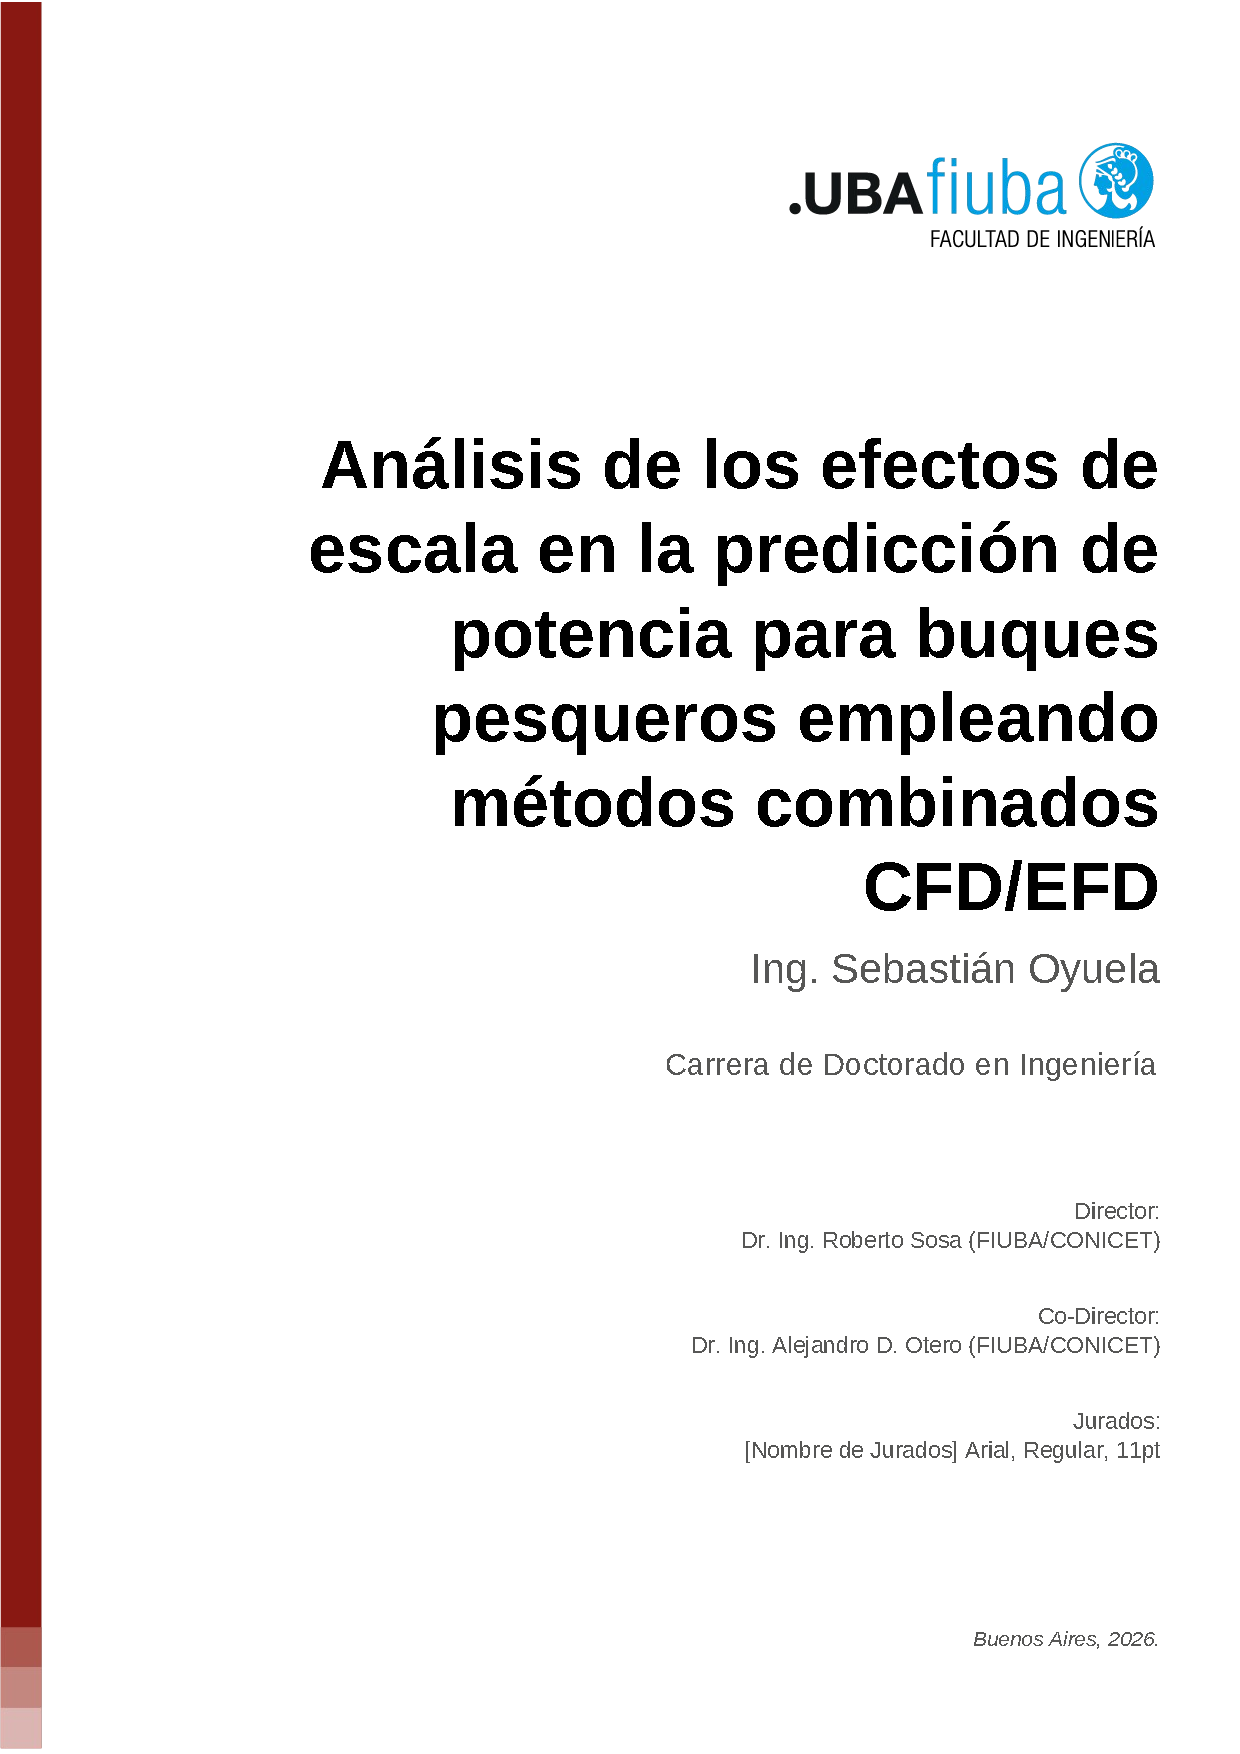
\includepdf{images/Caratula_Tesis_Doctorado.pdf}

\section*{Resumen}

La tesis aborda los efectos de escala en la extrapolación modelo--buque, un
problema central de la hidrodinámica naval derivado de la imposibilidad de
igualar simultáneamente los adimensionales entre modelo y buque real. El trabajo
se basa en una metodología combinada CFD--EFD: por un lado, simulaciones CFD
(RANS, con modelos de turbulencia SST y de transición SST-LM) sobre cascos de
pesqueros y hélices tipo Wageningen B4-60, entre otras; por otro, campañas
experimentales de resistencia y de hélices en aguas abiertas realizadas en canal
de ensayos, algunas propias y otras preexistentes en el LabHiNO (previas a la
tesis, o cedidas por una empresa), utilizadas para calibrar y validar los modelos
numéricos. Sobre la resistencia, se estudia en detalle el factor de forma $(1+k)$
de la hipótesis de Hughes: su determinación experimental y numérica combinada, la
influencia de la proa bulbo, la popa sumergida, la relación de aspecto $L/B$ del
casco, la línea de fricción de referencia (ITTC-57 vs.\ líneas numéricas) y el
modelo de turbulencia empleado, evaluando cómo cada uno de estos factores
introduce sesgos sistemáticos en la extrapolación a escala real.

En el capítulo de propulsión, la misma lógica de integración CFD--EFD se aplica al
análisis de los efectos de escala en hélices operando en aguas abiertas, mostrando
las limitaciones del procedimiento estándar ITTC-78 (que asume que toda la
diferencia entre escalas es friccional) frente a la evidencia, respaldada por
simulaciones, de que la componente de presión también escala de forma
significativa, cuantificada mediante la ``fracción de presión''. Se estudia además
el régimen transicional laminar-turbulento a bajos números de Reynolds de modelo,
donde la hipótesis del ITTC-78 falla al no contemplar el comportamiento no monótono
de $K_T/K_Q$, empleando el modelo de transición $\gamma$--$\widetilde{Re}_{\theta t}$
(SST-LM) calibrado y contrastado contra datos experimentales de campañas de aguas
abiertas. En síntesis, es una tesis de hidrodinámica naval con enfoque combinado
numérico--experimental, orientada a mejorar los procedimientos de extrapolación
modelo--buque tanto en resistencia como en propulsión.
\section*{Agradecimientos}
Quisiera agradecer encarecidamente a mi director de tesis Alejandro Otero y mi co-director Sebastián Oyuela por la inmensa ayuda que me proporcionaron durante todo el desarrollo de esta tesis. Sin su colaboración, este proyecto no hubiese sido posible. Agradezco también a Dimas Barile y Francisco García por sus consejos y contribuciones. Por último, expreso mi sincero agradecimiento al Centro de Simulación Computacional para Aplicaciones Tecnológicas por brindar el espacio y los recursos tecnológicos que posibilitaron el desarrollo de este trabajo.
\tableofcontents
\adjustmtc
\cleardoublepage
% ==========================================================================
%  NOMENCLATURA  —  colocar en el front matter (antes de la Introducción)
%  Requiere: \usepackage{longtable}
%  Tablas agrupadas por categoría. Adaptar/completar según capítulos finales.
% ==========================================================================

\chapter*{Nomenclatura}
\addcontentsline{toc}{chapter}{Nomenclatura}
\markboth{Nomenclatura}{Nomenclatura}

\renewcommand{\arraystretch}{1.25}

% --------------------------------------------------------------------------
\section*{Números adimensionales}
\begin{longtable}{@{}p{0.16\textwidth} p{0.78\textwidth}@{}}
$Fr$        & Número de Froude, $Fr = V/\sqrt{g\,L_{WL}}$ \\
$Fr_M,\,Fr_S$ & Número de Froude en escala modelo y buque \\
$Fr_{tr}$   & Número de Froude de la popa espejo, $Fr_{tr} = V/\sqrt{g\,T_{tr}}$ \\
$Re$        & Número de Reynolds, $Re = V L_{OS}/\nu$ \\
$Re_M,\,Re_S$ & Número de Reynolds en escala modelo y buque \\
$\overline{Re_M}$ & Número de Reynolds promedio en escala modelo (correlación de $k_{tr}$) \\
$Re_n$      & Número de Reynolds rotacional de la hélice, $Re_n = n D^2/\nu$ \\
$Re_{n,\mathrm{ref}}$ & Número de Reynolds rotacional de la escala de referencia \\
$Re_c$      & Número de Reynolds seccional de la hélice, $Re_c = c_{r/R}\,V_{\text{ref}}(r)/\nu$; se indica la sección empleada como $Re_{c,0.7R}$ o $Re_{c,0.75R}$ \\
$Re_{\theta t}$ & Número de Reynolds de transición basado en el espesor de cantidad de movimiento, obtenido de la correlación empírica en la corriente libre \\
$\widetilde{Re}_{\theta t}$ & Variable de transporte correspondiente a $Re_{\theta t}$ en el modelo de transición SST-LM \\
$y^+$       & Distancia adimensional a la pared, $y^+ = u_\tau y/\nu$ (primer centro de celda) \\
$Co,\,Co_{max}$ & Número de Courant, $Co = |\mathbf{U}|\,\Delta t/\Delta x$, y su valor máximo \\
$Tu$        & Intensidad turbulenta, $Tu = \sqrt{2k/3}\,/\,|\mathbf{U}|$, evaluada en el plano del disco de la hélice \\
$C_B$       & Coeficiente de bloque \\
$C_P$       & Coeficiente de presión sobre el casco, $C_P = (p-p_\infty)/\tfrac{1}{2}\rho V^2$ \\
$C_p$       & Coeficiente de presión sobre la pala, $C_p = (p-p_\infty)/\tfrac{1}{2}\rho V_{\text{ref}}^2$, con $V_{\text{ref}}(r)$ la velocidad resultante en la sección de radio $r$ \\
$\Delta C_p$ & Diferencia del coeficiente de presión sobre la pala entre escalas, $\Delta C_p = C_p(Re_n) - C_p(Re_{n,\mathrm{ref}})$ \\
$C_f$       & Coeficiente de fricción local sobre la pala, $C_f = |\boldsymbol{\tau}_w|/\tfrac{1}{2}\rho V_{\text{ref}}^2$ \\
\end{longtable}

\noindent{\footnotesize Los coeficientes referidos al casco se denotan con subíndice mayúscula ($C_P$, $C_F$) y los referidos a la pala del propulsor con subíndice minúscula ($C_p$, $C_f$).\par}

% --------------------------------------------------------------------------
\section*{Coeficientes y fuerzas de resistencia}
\begin{longtable}{@{}p{0.16\textwidth} p{0.78\textwidth}@{}}
$C_T$              & Coeficiente de resistencia total \\
$C_{TM},\,C_{TS}$  & Coeficiente de resistencia total en escala modelo y buque \\
$C_F$              & Coeficiente de resistencia friccional \\
$C_{F0}$           & Coeficiente de fricción de referencia (línea ITTC-57) \\
$C_{FM0},\,C_{FS0}$& Coeficiente de fricción de referencia en escala modelo y buque \\
$C_V$              & Coeficiente de resistencia viscosa, $C_V = C_F + C_{PV}$ \\
$C_{PV}$           & Coeficiente de resistencia por presión viscosa \\
$C_W$              & Coeficiente de resistencia por formación de olas \\
$C_R$              & Coeficiente de resistencia residual (componente no friccional en la descomposición de Hughes/Froude) \\
$\Delta C_F$       & Corrección por rugosidad de la superficie (Townsin \& Dey) \\
$C_A$              & Coeficiente de correlación modelo--buque \\
$C_{AAS}$          & Coeficiente de resistencia aerodinámica de la obra muerta \\
$C_{tr,S}$         & Coeficiente de resistencia asociado al espejo de popa a escala buque \\
$R_T$              & Fuerza de resistencia total \\
$R_{TM},\,R_{TS}$  & Fuerza de resistencia total en escala modelo y buque \\
$R_V$              & Resistencia viscosa \\
$R_F$              & Resistencia friccional \\
$R_{PV}$           & Resistencia por presión viscosa \\
$R_W$              & Resistencia por formación de olas \\
$k,\;(1+k)$        & Factor de forma \\
$k_M,\,k_S$        & Factor de forma en escala modelo y buque \\
$k_{tr}$           & Factor de forma del espejo \\
$V$                & Velocidad de avance del buque o modelo \\
$V_M,\,V_S$        & Velocidad de avance en escala modelo y buque \\
$q$                & Presión dinámica, $q = \tfrac{1}{2}\rho V^2$ \\
$P_{ES}$           & Potencia efectiva a escala buque, $P_{ES} = R_{TS}V_S$ \\
\end{longtable}

% --------------------------------------------------------------------------
\section*{Geometría del casco y del espejo}
\begin{longtable}{@{}p{0.16\textwidth} p{0.78\textwidth}@{}}
$L_{WL}$    & Eslora en flotación \\
$L_{PP}$    & Eslora entre perpendiculares \\
$L_{OS}$    & Eslora total sumergida \\
$B$         & Manga \\
$T$         & Calado \\
$S$         & Área de superficie mojada \\
$\nabla$    & Volumen de desplazamiento \\
$\Delta$    & Desplazamiento (masa) \\
$\lambda$   & Razón de escala geométrica \\
$L/B$       & Relación de esbeltez (eslora--manga) \\
$k_s$       & Altura de rugosidad equivalente \\
$A_{tr}$    & Área del espejo sumergido \\
$A_{\max}$  & Área máxima de la sección transversal \\
$T_{tr}$    & Inmersión efectiva del borde inferior del espejo \\
$y_{tr}$    & Semimanga en la intersección del espejo con la superficie libre \\
$tr_{\text{ratio}}$    & Relación entre el área del espejo sumergido y la sección maestra, $A_{tr}/A_{\max}$ \\
$tr_{\text{fullness}}$ & Coeficiente de llenado del espejo, $A_{tr}/(2\,y_{tr}\,T_{tr})$ \\
\end{longtable}

% --------------------------------------------------------------------------
\section*{Propulsión (hélices en aguas abiertas)}
\begin{longtable}{@{}p{0.16\textwidth} p{0.78\textwidth}@{}}
$K_T$       & Coeficiente de empuje, $K_T = T/(\rho n^2 D^4)$ \\
$K_{TM},\,K_{TS}$ & Coeficiente de empuje en escala modelo y buque \\
$K_Q$       & Coeficiente de torque, $K_Q = Q/(\rho n^2 D^5)$ \\
$K_{QM},\,K_{QS}$ & Coeficiente de torque en escala modelo y buque \\
$K_{Tp},\,K_{Tf}$ & Componentes de presión y de fricción del coeficiente de empuje \\
$K_{Qp},\,K_{Qf}$ & Componentes de presión y de fricción del coeficiente de torque \\
$\Delta K_T$      & Incremento del coeficiente de empuje entre escalas, $\Delta K_T = K_{TS}-K_{TM}$. El procedimiento ITTC-78 emplea la convención de signo opuesta \\
$\Delta K_Q$      & Corrección de escala sobre el coeficiente de torque \\
$\Delta K_{Tp},\,\Delta K_{Tf}$ & Componentes de presión y de fricción del efecto de escala sobre $K_T$ \\
$\Delta K_{Qp},\,\Delta K_{Qf}$ & Componentes de presión y de fricción del efecto de escala sobre $K_Q$ \\
$\delta K_T,\,\delta K_Q$ & Diferencia entre el cálculo sensible a la transición y el totalmente turbulento, a escala e igual punto de funcionamiento fijos \\
$\delta K_{Tp},\,\delta K_{Tf}$ & Componentes de presión y de fricción de $\delta K_T$ \\
$\delta K_{Qp},\,\delta K_{Qf}$ & Componentes de presión y de fricción de $\delta K_Q$ \\
$f_p$       & Fracción de presión del efecto de escala, $f_p = \Delta K_{Tp}/\Delta K_T$ \\
$J$         & Coeficiente de avance, $J = V_a/(nD)$ \\
$\eta_0$    & Rendimiento en aguas abiertas \\
$\eta_{0M},\,\eta_{0S}$ & Rendimiento en aguas abiertas en escala modelo y buque \\
$T$         & Empuje \\
$T_p,\,T_f$ & Componentes de presión y de fricción del empuje \\
$Q$         & Torque \\
$Q_p,\,Q_f$ & Componentes de presión y de fricción del torque \\
$n$         & Velocidad de giro [rev/s] \\
$D$         & Diámetro de la hélice \\
$R$         & Radio de la pala, $R = D/2$ \\
$r$         & Coordenada radial medida desde el eje \\
$r/R$       & Posición radial adimensional \\
$V_a$       & Velocidad de avance del propulsor, $V_a = J\,n\,D$ \\
$V_{\text{ref}}(r)$ & Velocidad resultante del flujo incidente en la sección de radio $r$, $V_{\text{ref}}(r)=\sqrt{V_a^2+(2\pi n r)^2}$ \\
$V_{0.7R}$  & Velocidad resultante en la sección $r/R=0{,}7$ \\
$Z$         & Número de palas \\
$A_E,\,A_0$ & Área expandida de las palas y área del disco \\
$A_E/A_0$   & Relación de área expandida \\
$A_b$       & Superficie del álabe (dominio de integración de fuerzas) \\
$P$         & Paso geométrico \\
$P/D$       & Relación paso--diámetro \\
$c_{r/R}$   & Cuerda de la sección en la posición radial $r/R$ \\
$c_{0.7R},\,c_{0.75R}$ & Cuerda de la sección a $r/R=0{,}7$ y $r/R=0{,}75$ \\
$t_{\max}$  & Espesor máximo de la sección de pala \\
$k_{s,p}$   & Rugosidad equivalente de la pala (ITTC-78) \\
$x/c$       & Coordenada adimensional a lo largo de la cuerda de la sección \\
$C_{D,M},\,C_{D,S}$ & Coeficiente de arrastre de perfil en escala modelo y buque (ITTC-78) \\
$\Delta C_D$& Corrección de arrastre de perfil (ITTC-78) \\
\end{longtable}

% --------------------------------------------------------------------------
\section*{Modelado numérico y turbulencia}
\begin{longtable}{@{}p{0.16\textwidth} p{0.78\textwidth}@{}}
$U_i,\,\mathbf{U}$ & Componente $i$ de la velocidad media y su forma vectorial \\
$u_i'$      & Fluctuación turbulenta de la velocidad \\
$x_i$       & Coordenada espacial \\
$x,\,y,\,z$ & Coordenadas longitudinal, transversal y vertical; $z$ positiva hacia arriba desde la flotación estática. En capa límite, $y$ denota la distancia normal a la pared \\
$t$         & Tiempo \\
$\Delta t,\,\Delta x$ & Paso temporal y tamaño local de celda \\
$p,\,p_\infty$ & Presión estática local y presión de la corriente no perturbada \\
$p_{rgh}$   & Presión modificada, $p_{rgh}=p-\rho g_j x_j$ \\
$g,\,g_i$   & Aceleración de la gravedad y su componente $i$ \\
$\alpha_{water}$ & Fracción volumétrica de agua (VoF) \\
$\rho$      & Densidad del fluido \\
$\nu$       & Viscosidad cinemática molecular \\
$\nu_t$     & Viscosidad cinemática turbulenta \\
$\mu,\,\mu_t$ & Viscosidad dinámica molecular y turbulenta \\
$k$         & Energía cinética turbulenta \\
$\omega$    & Tasa específica de disipación \\
$\varepsilon$ & Tasa de disipación turbulenta \\
$k_L$       & Energía cinética de las fluctuaciones laminares (modelo $k$-$k_L$-$\omega$) \\
$\tau_w,\,\boldsymbol{\tau}_w$ & Esfuerzo cortante de pared y su forma vectorial \\
$u_\tau$    & Velocidad de fricción, $u_\tau=\sqrt{\tau_w/\rho}$ \\
$\mathbf{n}$ & Versor normal exterior a la superficie \\
$\hat{\mathbf{e}}_x$ & Versor en la dirección de avance \\
$\delta_{ij}$ & Delta de Kronecker \\
$\gamma$    & Intermitencia (variable de transporte del modelo de transición SST-LM) \\
$F_1,\,F_2$ & Funciones de mezcla del modelo SST \\
$\tilde{P}_k$ & Término de producción limitado de turbulencia \\
$S_{ij},\,S$& Tensor y magnitud de la tasa de deformación \\
$a_1$       & Constante de Bradshaw ($=0{,}31$) \\
$\alpha,\,\beta,\,\beta^*$ & Coeficientes de cierre del modelo $k$--$\omega$ SST \\
$\sigma_k,\,\sigma_\omega,\,\sigma_{\omega 2}$ & Coeficientes de difusión del modelo $k$--$\omega$ SST \\
$C_\mu$     & Constante del modelo $k$--$\varepsilon$ ($=0{,}09$) \\
$C_{\varepsilon 1},\,C_{\varepsilon 2}$ & Constantes del modelo $k$--$\varepsilon$ \\
$\sigma_\varepsilon$ & Coeficiente de difusión de $\varepsilon$ \\
$Q$         & Segundo invariante del gradiente de velocidad (criterio Q) \\
\end{longtable}

% --------------------------------------------------------------------------
\section*{Verificación, validación e incertidumbre}
\begin{longtable}{@{}p{0.16\textwidth} p{0.78\textwidth}@{}}
$GCI$       & Índice de convergencia de malla (\textit{Grid Convergence Index}) \\
$R$         & Razón de convergencia \\
$p$         & Orden aparente de precisión \\
$r$         & Razón de refinamiento de malla \\
$h$         & Tamaño característico de celda \\
$\Phi$      & Variable de interés en el estudio de convergencia \\
$\epsilon$  & Diferencia de la solución entre mallas sucesivas \\
$F_s$       & Factor de seguridad ($=1{,}25$) \\
$u_i$       & Componente $i$ de incertidumbre estándar \\
$u_c$       & Incertidumbre estándar combinada \\
$k_c$       & Factor de cobertura ($=2$) \\
$U_{95}$    & Incertidumbre expandida (nivel de confianza del 95\,\%) \\
$N$         & Número de repeticiones de un ensayo o de puntos de comparación \\
$E\%D$      & Error de comparación, $E\%D = (D-S)/D\times100$ \\
$D$         & Valor experimental (\textit{data}) \\
$S$         & Resultado computacional (\textit{simulation}) \\
$U_D$       & Incertidumbre experimental \\
$U_{num}$   & Incertidumbre numérica \\
$U_{val}$   & Incertidumbre de validación, $U_{val}=\sqrt{U_D^2+U_{num}^2}$ \\
MAE         & Error absoluto medio (\textit{Mean Absolute Error}) \\
\end{longtable}

% --------------------------------------------------------------------------
\section*{Acrónimos}
\begin{longtable}{@{}p{0.16\textwidth} p{0.78\textwidth}@{}}
CFD     & \textit{Computational Fluid Dynamics} (dinámica de fluidos computacional) \\
EFD     & \textit{Experimental Fluid Dynamics} (dinámica de fluidos experimental) \\
RANS    & \textit{Reynolds-Averaged Navier--Stokes} \\
SST     & \textit{Shear Stress Transport} (modelo de turbulencia) \\
SST-LM  & Modelo de transición SST de Langtry--Menter ($\gamma$-$\widetilde{Re}_{\theta t}$) \\
EASM    & \textit{Explicit Algebraic Stress Model} (modelo de esfuerzos algebraico explícito) \\
VoF     & \textit{Volume of Fluid} \\
MULES   & \textit{Multidimensional Universal Limiter for Explicit Solution} (compresión de interfaz en VoF) \\
FVM     & Método de volúmenes finitos (\textit{Finite Volume Method}) \\
SIMPLE  & \textit{Semi-Implicit Method for Pressure-Linked Equations} \\
PISO    & \textit{Pressure-Implicit with Splitting of Operators} \\
PIMPLE  & Algoritmo híbrido PISO--SIMPLE \\
MRF     & Marco de referencia múltiple (\textit{Multiple Reference Frame}) \\
AMI     & Interfaz de malla arbitraria (\textit{Arbitrary Mesh Interface}) \\
DB      & Doble cuerpo (\textit{double body}) \\
NFL     & Línea de fricción numérica (\textit{Numerical Friction Line}) \\
ITTC    & \textit{International Towing Tank Conference} \\
ITTC-57 & Línea de correlación modelo--buque de la ITTC (1957) \\
ITTC-78 & Método de predicción de potencia de la ITTC (1978) \\
GCI     & Índice de convergencia de malla \\
V\&V    & Verificación y validación \\
MAE     & Error absoluto medio (\textit{Mean Absolute Error}) \\
RSS     & Raíz de la suma de los cuadrados (\textit{Root Sum Squares}) \\
RMS     & Raíz del valor cuadrático medio (\textit{Root Mean Square}) \\
POW     & Ensayo de hélice en aguas abiertas (\textit{Propeller Open Water}) \\
BPG     & Guías de buenas prácticas (\textit{Best Practice Guidelines}) \\
LCB     & Centro longitudinal de carena (\textit{Longitudinal Centre of Buoyancy}) \\
KRISO   & \textit{Korea Research Institute of Ships and Ocean Engineering} \\
KCS     & \textit{KRISO Container Ship} \\
KVLCC2  & \textit{KRISO Very Large Crude Carrier}, versión 2 \\
LabHiNO & Laboratorio de Hidrodinámica Naval y Oceánica (UBA) \\
UBA     & Universidad de Buenos Aires \\
MARIN   & \textit{Maritime Research Institute Netherlands} \\
ASME    & \textit{American Society of Mechanical Engineers} \\
IMO     & \textit{International Maritime Organization} \\
\end{longtable}

\renewcommand{\arraystretch}{1.0}
\chapter{Introducción general}
\mtcsettitle{minitoc}{Contenidos} 
\minitoc
\section{Contexto y motivación del estudio}
\label{sec:contexto}

\subsection{Orígenes de la pesca comercial y de la industria naval pesquera en Argentina}

La actividad pesquera comercial en Argentina cuenta con antecedentes documentados
desde 1821, con un primer polo de desarrollo en Puerto Rawson, en la provincia de
Chubut \citep{phantom_pesca_argentina}. Sin embargo, el despegue de la pesca como
industria organizada se produce recién en el siglo~XX, de la mano de la
inmigración europea, principalmente española e italiana, que se asentó en
Mar del Plata en las décadas posteriores a la Segunda Guerra Mundial
\citep{phantom_pesca_argentina}. Aquellos primeros pescadores operaban
embarcaciones artesanales, en algunos casos aún propulsadas a vela, orientadas a
capturas de especies pelágicas de media agua (anchoíta, caballa, bonito) que
alimentaron una incipiente industria conservera. El crecimiento del puerto de
Mar del Plata, inaugurado oficialmente en 1922, y la consolidación de sus
escolleras, ordenaron el espacio necesario para que talleres, varaderos y
astilleros artesanales fueran naciendo alrededor de la actividad
\citep{confluencia_portuaria_mdp}. Familias de inmigrantes, como la de Luis
Solimeno, instalado en la ciudad en 1942, contribuyeron decisivamente a
convertir a Mar del Plata en el principal puerto pesquero del país
\citep{argenports_solimeno}.

El salto tecnológico hacia una flota de mayor porte y capacidad se dio a
mediados de la década de 1960, cuando los empresarios Francisco ``Paco''
Ventura y José Greco introdujeron en el mercado interno el filet fresco de
merluza. En 1965, Greco encargó la construcción de cuatro buques de acero en
astilleros de Buenos Aires, cada uno con capacidad para transportar entre
1500 y 2000 cajones de pescado \citep{phantom_pesca_argentina}, marcando el
inicio de una flota industrial de altura construida en el país. El Estado
argentino acompañó, de manera intermitente, este proceso mediante líneas de
crédito blando para la construcción de buques y la incorporación de
tecnología, desde el Decreto 10032/66 del Banco Industrial hasta,
décadas más tarde, el Decreto 145/2019 sobre Lineamientos para la Renovación
de la Flota \citep{phantom_pesca_argentina}.

La industria pesquera nacional experimentó un fuerte crecimiento durante la
década de 1990, impulsado tanto por el aumento del número de buques como por
su mayor potencial de captura: las capturas marítimas totales pasaron de
545 mil toneladas en 1990 a 1{,}34 millones de toneladas en 1997
\citep{rotoplas_historia_pesca}. Este período estuvo acompañado por la
consolidación de la soberanía nacional sobre los recursos vivos de la Zona
Económica Exclusiva argentina y por políticas de fomento a la radicación de
plantas procesadoras, particularmente en la Patagonia
\citep{pesca_maritima_1989_2013}.

Paralelamente, la industria de construcción naval argentina, de la cual la
construcción de buques pesqueros es hoy uno de sus segmentos más dinámicos,
tiene antecedentes que se remontan a la época colonial: el primero data de
1520, cuando Hernando de Magallanes estableció un taller de reparaciones en
la ría de San Julián, y en 1527 se instaló un astillero en el Fuerte Sancti
Spiritu, sobre el río Paraná \citep{argentina_gob_industria_naval}. Ya en el
siglo~XX, hitos como la creación de los Talleres Navales de La Boca en 1936 y
la instalación de infraestructura de reparación sobre el río Luján
consolidaron un sector que, sin embargo, sufrió una crisis profunda a
comienzos de la década de 1990 con la disolución de la flota estatal, el
cierre de numerosos astilleros y talleres, y la pérdida de competitividad
frente a los astilleros asiáticos \citep{padua_construccion_naval}. La
derogación, hacia fines de esa década, del régimen que permitía el
arrendamiento de buques extranjeros para el cabotaje nacional dio inicio a un
proceso de recuperación que, en el segmento pesquero, se profundizó
notablemente en los últimos años.

\subsection{Estado actual de la industria pesquera y de la industria naval pesquera nacional}

La pesca continúa siendo hoy uno de los complejos exportadores más relevantes
de la economía argentina. Según datos de la Subsecretaría de Pesca y
Acuicultura, en 2025 el sector generó divisas por 2010 millones de dólares, un incremento del 4{,}3\,\% respecto de 2024, sobre un total de 549\,416
toneladas exportadas, constituyendo el segundo mejor registro histórico del
complejo pesquero nacional, solo superado por el récord de 2018
\citep{argentina_gob_pesca_2025}. El langostino patagónico (\textit{Pleoticus
muelleri}) es el principal producto de exportación, con 867 millones de
dólares y 119\,775 toneladas en 2025, a un precio promedio de 7240
dólares por tonelada; le siguen el calamar (\textit{Illex argentinus}), cuyas
exportaciones crecieron un 32{,}5\,\% en valor respecto del año anterior, y la
merluza (\textit{Merluccius hubbsi}), con 326 millones de dólares y 127\,422
toneladas \citep{pescare_exportaciones_2025}. China, España y Estados Unidos
concentraron en conjunto algo más de la mitad de las exportaciones pesqueras
argentinas de ese año \citep{argentina_gob_pesca_2025}.

Este dinamismo exportador, sostenido en gran medida por el crecimiento de la
pesquería de langostino (que pasó de capturas del orden de las 20\,000
toneladas anuales a picos de más de 250\,000 toneladas en apenas un par de
décadas, al punto de ser denominado por actores del sector como ``la soja de
la pesca''), tuvo un correlato directo sobre la industria naval nacional
\citep{argenports_industria_naval}. Astilleros que hasta entonces se dedicaban
exclusivamente a la reparación debieron encarar obras de infraestructura para
comenzar a construir buques nuevos; astilleros del Delta del Paraná y de
Tigre que tradicionalmente construían embarcaciones de turismo o barcazas
incursionaron por primera vez en la construcción de buques pesqueros, y
establecimientos que habían permanecido inactivos durante años fueron
reactivados \citep{argenports_industria_naval}. En la actualidad, el sector de
la industria naval argentina (que incluye, además del segmento pesquero, la
reparación y construcción para otros usos) se compone de más de 300 empresas
y emplea a alrededor de 10\,000 trabajadores en forma directa
\citep{argenports_industria_naval}.

El polo naval pesquero más importante del país se encuentra en el puerto de
Mar del Plata, donde operan, entre otros, el Astillero Naval Federico
Contessi y Cía.\ S.A. (especializado desde hace décadas en la construcción de
buques pesqueros costeros, de altura, congeladores, palangreros y tangoneros
\citep{contessi_historia}), Astilleros Servicios Portuarios Integrados S.A.
(SPI) y TecnoPesca Argentina (TPA), astilleros a los que en 2023 la autoridad
portuaria otorgó concesiones a veinte años para desarrollar nuevas obras de
infraestructura, en el marco del crecimiento sostenido de la demanda de
construcción de embarcaciones nuevas \citep{globalports_concesiones_mdp}. A
ellos se suman astilleros de otras localidades del litoral marítimo y
fluvial, entre los que se destaca el astillero de la firma JPA~S.A., y
emprendimientos más recientes como Astilleros Patagónicos Integrados, que
buscan descentralizar hacia el sur la capacidad de construcción y reparación
naval \citep{pescare_api_patagonia}. Es en este contexto de renovación de
flota (con nuevas unidades de mayor porte y complejidad, construidas
íntegramente en el país) que se enmarca el interés de la presente tesis: los
buques pesqueros analizados son representativos de dicho proceso.

A pesar de esta vitalidad productiva, la predicción de potencia y el diseño
hidrodinámico de estos buques continúan apoyándose, en gran medida, en
metodologías de extrapolación modelo--buque desarrolladas y validadas
históricamente sobre buques mercantes esbeltos. Los pesqueros que hoy se
construyen en el país pertenecen, en cambio, a una tipología de casco de baja
esbeltez, es decir, de relación eslora-manga reducida ($L/B < 4$, donde $L$ es
la eslora y $B$ la manga), cuyas proporciones difieren sustancialmente de las
de aquellos cascos. Esta tipología no es, sin embargo, una particularidad de
la flota argentina: las series sistemáticas clásicas de buques pesqueros,
desarrolladas en distintos países, incluyen cascos de proporciones similares
\citep{yilmaz1999}, lo que evidencia su amplia difusión internacional. Esta
situación motiva la problemática que se desarrolla en la siguiente sección.

\section{Problemática de los efectos de escala en la predicción de potencia}
\label{sec:problematica}

La problemática que aborda esta tesis presenta dos niveles que conviene
distinguir. El primero es general: los efectos de escala son inherentes a
toda predicción de potencia basada en ensayos con modelos, cualquiera sea la
geometría del buque o del propulsor. El segundo es particular: los métodos
tradicionales con los que se corrigen esos efectos pueden no resultar
adecuados para tipologías de casco alejadas de aquellas sobre las que fueron
desarrollados, como es el caso de los buques pesqueros de baja esbeltez.

\subsection{Los efectos de escala como problema general}

La predicción de la potencia de un buque a partir de ensayos con modelos
físicos obliga a extrapolar resultados obtenidos a números de Reynolds muy
inferiores a los de operación del buque. Esta falta de semejanza dinámica
completa entre modelo y buque, presente en todo ensayo con modelos e
independiente de la forma del casco, da origen a los efectos de escala
(Capítulo~\ref{chap:antecedentes}). Estos afectan a las dos grandes
componentes de la predicción de potencia, que definen los dos ejes de esta
tesis: la resistencia al avance, cuya extrapolación descansa sobre el factor
de forma $(1+k)$ (un coeficiente que mide cuánto excede la resistencia viscosa
del casco a la de una placa plana equivalente), y la propulsión, en la que
los resultados de los ensayos de hélices en aguas abiertas deben escalarse a
los números de Reynolds de la hélice del buque.

Precisamente por su carácter general, estas dificultades han sido objeto de
atención sostenida por parte de la comunidad internacional de hidrodinámica
naval. El Comité Especialista en Métodos Combinados CFD/EFD (es decir,
métodos que integran simulaciones numéricas, CFD, y ensayos experimentales,
EFD) de la 29.ª ITTC (International Towing Tank Conference) relevó los problemas de escala que
afectan a la predicción de potencia y los calificó según su impacto sobre las
tendencias de diseño, su impacto sobre el valor absoluto de la potencia y la
frecuencia con que se presentan en la práctica, así como según la posibilidad
de mejorarlos mediante CFD \citep{ITTC_Combined_2021}. A partir de esa
evaluación, el comité propuso a la comunidad concentrar sus esfuerzos en cinco
temas, entre los cuales figuran los dos que constituyen los ejes de la
presente tesis: la determinación numérica del factor de forma y la mejora de
los métodos de escalado de los ensayos de hélices en aguas abiertas.

En el eje de la resistencia al avance, la determinación del factor de forma
obtuvo la calificación más alta de todos los temas evaluados, tanto por su
impacto como por su potencial de mejora mediante CFD. El comité señaló que el
procedimiento experimental habitual para obtenerlo (el método de Prohaska)
puede fallar para algunos tipos de buque, con errores del orden del 5\,\% y de
hasta el 10\,\% en la potencia total, y que puede además distorsionar las
tendencias de diseño, por ejemplo al comparar formas de casco alternativas.
Por esas razones, seleccionó este tema para un estudio colaborativo
específico, cuyos resultados se discuten en el
Capítulo~\ref{chap:antecedentes}.

En el eje de la propulsión, el comité subrayó que el escalado de los
resultados del ensayo de aguas abiertas a otros números de Reynolds es una
parte crucial de la predicción de potencia y que, si bien el procedimiento
ITTC-78 ofrece formulaciones sencillas para ello, los distintos métodos
disponibles conducen a resultados significativamente diferentes. Identificó,
además, dos dificultades de fondo: la presencia de flujo laminar y de
transición laminar--turbulenta sobre las palas a escala de modelo, cuya
simulación numérica sigue siendo una tarea exigente, y la dependencia del
efecto de escala con la geometría de la pala, que afecta especialmente a
diseños no convencionales, como las hélices de área de pala reducida. En su
evaluación, este tema recibió la calificación máxima en impacto sobre las
tendencias de diseño y en frecuencia de aparición, aunque un impacto menor
sobre el valor absoluto de la potencia, con errores estimados de hasta un
3\,\% que pueden conducir a diseños de hélice subóptimos en los tipos de buque
más comunes. El comité concluyó que se requieren nuevos estudios, en los que
el CFD puede formar parte, para eventualmente actualizar el procedimiento de
escalado recomendado por la ITTC \citep{ITTC_Combined_2021}.

\subsection{Limitaciones de los métodos tradicionales en buques de baja esbeltez}

A los efectos de escala comunes a cualquier buque se suma un problema
particular de ciertas tipologías de casco. Los métodos tradicionales de
extrapolación modelo--buque, así como las correlaciones empíricas asociadas
a ellos, fueron desarrollados y calibrados fundamentalmente sobre buques
mercantes esbeltos, y la evidencia que respalda el enfoque combinado EFD--CFD
proviene, hasta el momento, de cascos de referencia de esbeltez moderada
(Capítulo~\ref{chap:antecedentes}). La propia ITTC advierte que, si bien los
errores de estos métodos quedan en promedio bien compensados por las
correlaciones de cada canal de ensayos cuando se trabaja con tipos de buque
habituales, pueden ser mayores para buques que se apartan de esos tipos
\citep{ITTC_Combined_2021}. Su aplicabilidad a cascos de baja relación
eslora-manga, como los de los buques pesqueros, no está por lo tanto
garantizada, y su uso sin una verificación específica puede conducir a
errores significativos en la predicción de potencia.

\subsection{Enfoque y alcance de la tesis}

En correspondencia con estos dos niveles, la tesis persigue un propósito
también doble. En primer lugar, contribuir de manera general al estudio de los
efectos de escala mediante métodos combinados EFD--CFD en los dos ejes
señalados por la ITTC: en el de la resistencia al avance, a través de la
determinación del factor de forma y de su dependencia con la escala, y en el
de la propulsión, a través del escalado de las hélices en aguas abiertas,
tanto en régimen turbulento como en presencia de transición a escala de
modelo. Estos aportes no se restringen a una tipología particular, ya que se
apoyan también en un buque y en hélices de referencia. En segundo lugar,
examinar en particular qué ocurre en el eje de la resistencia al avance con
los buques pesqueros de baja esbeltez, tomando como casos de estudio tres
pesqueros diseñados y construidos en astilleros argentinos, cuyos modelos
fueron ensayados en el canal de remolque del LabHiNO. Si bien los casos de
estudio provienen de la industria naval nacional, la difusión internacional de esta tipología de casco hace que sus resultados
sean de interés para buques pesqueros de proporciones similares en otras
flotas.

\section{Relevancia del estudio}

La predicción de la potencia propulsiva es una etapa central del proyecto de
un buque, ya que a partir de ella se seleccionan, en las etapas tempranas del
diseño, el motor principal y la hélice. Una subestimación de la potencia puede
dar lugar a un buque que no alcance la velocidad de servicio prevista o que
opere con márgenes insuficientes, mientras que una sobrestimación se traduce
en plantas propulsoras sobredimensionadas y en mayores costos de construcción
y de operación a lo largo de la vida útil del buque. La precisión de los
métodos de extrapolación modelo--buque tiene, por lo tanto, consecuencias
técnicas y económicas directas.

En el caso de los buques pesqueros, esa precisión depende de que los métodos
empleados resulten adecuados para cascos de baja esbeltez, cuyas proporciones
difieren de las de los buques sobre los que dichos métodos fueron
desarrollados. Caracterizar los efectos de escala en este tipo de cascos
contribuye, en consecuencia, a una predicción de potencia más confiable en
su diseño, tanto en el ámbito nacional como en el de otras flotas pesqueras
con buques de características similares.

\section{Objetivos generales y específicos}

La tesis se organiza en dos ejes, correspondientes a las dos grandes
componentes de la predicción de potencia, cada uno de ellos con su propio
objetivo general.

\subsection*{Objetivos generales}

\textbf{Eje 1. Resistencia al avance: factor de forma.} Caracterizar,
mediante métodos combinados EFD--CFD, los efectos de escala en la
determinación del factor de forma y su influencia en la predicción de la
resistencia al avance, con particular atención a los buques pesqueros de baja
esbeltez.

\textbf{Eje 2. Propulsión: hélices en aguas abiertas.} Caracterizar,
mediante métodos combinados EFD--CFD, los efectos de escala sobre las
prestaciones de hélices en aguas abiertas, tanto en régimen turbulento como
en presencia de transición laminar--turbulenta a escala de modelo.

\subsection*{Objetivos específicos}

\subsubsection*{Eje 1. Resistencia al avance: factor de forma}

\begin{itemize}
    \item Generar una base de datos experimental propia, obtenida en el canal
    de remolque del LabHiNO, de resistencia al avance para tres buques
    pesqueros de diseño nacional (P1, P2 y P3) y para un buque de referencia
    esbelto, el portacontenedores KCS (\textit{KRISO Container Ship}), uno de
    los cascos estándar de validación en hidrodinámica naval, que sirva de
    base de validación para las simulaciones numéricas.
    \item Determinar el factor de forma $(1+k)$ de dichos buques mediante los
    métodos de Prohaska y de doble cuerpo, contrastando ambos enfoques entre
    sí.
    \item Cuantificar la dependencia del factor de forma con el número de
    Reynolds sobre un rango de escalas geométricas que se extiende desde el
    modelo de ensayo hasta la escala buque, e identificar los mecanismos
    físicos responsables de dicha dependencia.
    \item Evaluar la validez de las hipótesis clásicas de extrapolación
    modelo--buque para cascos de baja esbeltez, a partir de los resultados
    obtenidos para los pesqueros P1, P2 y P3.
    \item Cuantificar el impacto de los efectos de escala identificados sobre
    la predicción de potencia efectiva a escala buque, en comparación con el
    procedimiento estándar de extrapolación de la ITTC.
\end{itemize}

\subsubsection*{Eje 2. Propulsión: hélices en aguas abiertas}

\begin{itemize}
    \item Caracterizar los efectos de escala sobre los coeficientes
    hidrodinámicos de una hélice de referencia de la serie Wageningen~B (una
    familia sistemática y ampliamente documentada de hélices, de uso estándar
    como referencia) en aguas abiertas, desde la escala de modelo hasta la
    escala buque, y compararlos con las predicciones del procedimiento
    estándar ITTC-78.
    \item Evaluar sobre una hélice de diseño convencional, pero no seriada,
    cedida por un proveedor privado, el comportamiento en condiciones clásicas
    de ensayo a escala de modelo y los efectos asociados al régimen de
    transición laminar--turbulenta, que se manifiesta cuando la capa límite
    sobre los álabes opera a números de Reynolds bajos con regiones laminares
    de extensión significativa.
    \item Cuantificar el impacto de los efectos de escala identificados sobre
    la predicción de las prestaciones de la hélice a escala buque, en
    comparación con el procedimiento ITTC-78.
\end{itemize}

\section{Estructura de la tesis}

El resto de la tesis se organiza en cinco capítulos adicionales. El
Capítulo~\ref{chap:antecedentes} desarrolla los fundamentos teóricos de la
similitud dinámica y el estado del arte sobre el factor de forma, su
determinación asistida por simulaciones numéricas y los efectos de escala en
hélices, sentando el marco conceptual sobre el que se apoya el resto del
trabajo. El Capítulo~\ref{chap:Metodologia} describe en detalle las
instalaciones experimentales del LabHiNO, los modelos físicos ensayados, el
procedimiento de extrapolación modelo--buque y la configuración numérica
empleada en OpenFOAM, tanto para las simulaciones de resistencia del casco
(con superficie libre y en configuración de doble cuerpo) como para el
análisis de la hélice en aguas abiertas, además de la estrategia de
verificación y validación adoptada. El
Capítulo~\ref{cap:resistencia_factor_de_forma} desarrolla el Eje~1:
presenta el análisis original de resistencia al avance y factor de forma para el buque pesquero P1 y su
buque de referencia KCS, incluyendo el estudio de los efectos de escala y la
influencia de la proa bulbo, la popa sumergida, el modelo de turbulencia y la
relación $L/B$, extendiendo finalmente el análisis a los pesqueros P2 y P3. El
Capítulo~\ref{chap:helices} desarrolla el Eje~2, correspondiente a la
segunda gran componente de la potencia propulsiva: presenta la validación y el análisis de efectos de escala de la
hélice de referencia Wageningen B4-60 y, sobre el propulsor P206, el estudio
de los efectos del régimen de transición laminar--turbulenta
a escala de modelo. Finalmente, el Capítulo~\ref{cap:conclusiones_generales}
integra los resultados de resistencia y propulsión, discute su impacto sobre
la predicción de potencia y sobre la práctica de diseño y ensayo de buques
pesqueros, resume los aportes principales y propone líneas de trabajo futuro.

% -----------------------------------------------------------------------
% NOTA PARA EL AUTOR: Las siguientes claves de cita fueron construidas a
% partir de las fuentes consultadas para esta sección y deben agregarse
% a la base .bib del proyecto (o reemplazarse por las claves ya
% existentes si alguna de estas fuentes ya estuviera citada):
%   phantom_pesca_argentina, confluencia_portuaria_mdp,
%   argenports_solimeno, rotoplas_historia_pesca,
%   pesca_maritima_1989_2013, argentina_gob_industria_naval,
%   padua_construccion_naval, argentina_gob_pesca_2025,
%   pescare_exportaciones_2025, argenports_industria_naval,
%   contessi_historia, globalports_concesiones_mdp,
%   pescare_api_patagonia
% -----------------------------------------------------------------------
\chapter{Antecedentes y estado del arte}
\label{chap:antecedentes}
\mtcsettitle{minitoc}{Contenidos} 
\minitoc
 
 
\section{Resistencia al avance. El problema de la extrapolación modelo--buque}
\label{sec:extrapolacion}

La predicción de la resistencia al avance de un buque a escala buque a partir de ensayos con modelos físicos se basa en la \textbf{similitud dinámica}. Dos flujos alrededor de cuerpos geométricamente semejantes son dinámicamente similares si comparten los mismos grupos adimensionales que gobiernan la física del flujo. Para el caso de un buque de superficie en aguas tranquilas, las ecuaciones de Navier-Stokes adimensionalizadas revelan dos parámetros fundamentales: el \textbf{número de Reynolds} $Re = VL/\nu$, que expresa la relación entre fuerzas inerciales y viscosas, y el \textbf{número de Froude} $Fr = V/\sqrt{gL}$, que expresa la relación entre fuerzas inerciales y gravitatorias. En ambos parámetros, $V$ es la velocidad de avance, $L$ la eslora característica, $\nu$ la viscosidad cinemática del agua y $g$ la aceleración de la gravedad. En esta tesis se adopta $L = L_{OS}$, la eslora total sumergida, para el número de Reynolds, por ser la longitud sobre la que efectivamente se desarrolla la capa límite, y $L = L_{WL}$, la eslora en flotación, para el número de Froude, por ser la que gobierna el tren de olas generado. La similitud dinámica completa requeriría igualdad simultánea de ambos parámetros entre modelo ($M$) y buque ($S$):
%
\begin{equation}
    Re_M = Re_S \qquad \text{y} \qquad Fr_M = Fr_S.
\end{equation}
%
Sin embargo, al utilizar agua en ambas escalas ($\nu_M \approx \nu_S$, $g_M = g_S$), estas dos condiciones imponen escalas de velocidad contradictorias. La igualdad de Froude exige $V_M = V_S / \sqrt{\lambda}$, mientras que la igualdad de Reynolds exige $V_M = V_S \cdot \lambda$, siendo $\lambda = L_S / L_M$ el factor de escala lineal. Para valores típicos de $\lambda$ entre 20 y 80, es imposible satisfacer ambas condiciones simultáneamente con agua como fluido de trabajo \citep{birk2019}.

La solución práctica, establecida históricamente por William Froude, consiste en respetar la similitud de Froude durante los ensayos (capturando correctamente la generación de olas) y corregir analíticamente la diferencia en la componente viscosa. Esta \textbf{similitud dinámica parcial} introduce los denominados ``efectos de escala'': diferencias sistemáticas entre el flujo de modelo y el del buque que no están capturadas por la extrapolación estándar y que constituyen la problemática central de esta tesis.

Para cuantificar la resistencia de manera independiente de la escala, se trabaja con el \textbf{coeficiente adimensional de resistencia total}:
%
\begin{equation}\label{eq:CT}
    C_T = \frac{R_T}{\tfrac{1}{2}\,\rho\,V^2\,S},
\end{equation}
%
donde $R_T$ es la fuerza de resistencia total, $\rho$ la densidad del agua
y $S$ la superficie mojada del casco. De manera
análoga se definen los coeficientes de resistencia viscosa $C_V$, friccional
$C_F$, por presión viscosa $C_{PV}$ y por formación de olas $C_W$, todos
referidos a la misma presión dinámica y superficie mojada. Los subíndices
$M$ y $S$ se utilizan a lo largo de esta tesis para distinguir las
magnitudes correspondientes al modelo y al buque respectivamente.

% ---------------------------------------------------------------------
% [REESCRITO] Planteo explícito de la no similitud: separación Re / Fr,
% hipótesis central de Hughes y forma final de C_TS.
% ---------------------------------------------------------------------
Con esta notación el problema de la no similitud puede plantearse de manera
precisa. El coeficiente de resistencia total es función de los dos parámetros
que gobiernan el flujo, $C_T = C_T(Re, Fr)$. El ensayo entrega un único valor
medido, $C_{TM}$, obtenido a $Fr_M = Fr_S$ pero a $Re_M \ll Re_S$: el punto
ensayado no es el punto que se desea predecir. Sin una hipótesis adicional el
dato experimental es, en rigor, inutilizable, porque nada permite discriminar
qué parte de $C_{TM}$ se modifica al pasar de $Re_M$ a $Re_S$ y qué parte
permanece. La extrapolación solo resulta posible si se postula que $C_T$ admite
una descomposición en dos términos \emph{separables}, uno función exclusiva del
número de Reynolds y otro función exclusiva del número de Froude. La propuesta de
\citet{hughes1954} le da forma concreta a esa separación:
%
\begin{equation}\label{eq:CT_decomposicion_hughes}
    C_T(Re,Fr) = (1+k)\,C_{F0}(Re) + C_W(Fr),
\end{equation}
%
donde $C_W$ es el coeficiente de resistencia por formación de olas, $C_{F0}$ es
el coeficiente de resistencia friccional adimensional de una \emph{placa plana
equivalente} --una placa plana bidimensional de la misma eslora y la misma
superficie mojada que el casco, evaluada al mismo número de Reynolds-- y $(1+k)$
es el \textbf{factor de forma}, un multiplicador de origen puramente geométrico.

El primer término de la Ecuación~\eqref{eq:CT_decomposicion_hughes} es la
resistencia viscosa total del casco,
%
\begin{equation}\label{eq:CV}
    C_V = C_F + C_{PV},
\end{equation}
%
que reúne la fricción $C_F$, integral de los esfuerzos de corte sobre la
superficie mojada, y la resistencia de presión viscosa $C_{PV}$, resultante de la
distribución de presiones que la propia capa límite modifica respecto de la del
flujo no viscoso. Ninguna de las dos existe sobre una placa plana en la misma
forma: el casco es tridimensional y curvo, de modo que su fricción es algo mayor
que la de la placa equivalente y, sobre todo, aparece una componente de presión
que la placa no tiene. La propuesta de Hughes consiste en afirmar que toda esa
diferencia puede absorberse en un único multiplicador geométrico,
%
\begin{equation}\label{eq:hughes}
    C_V = (1+k)\, C_{F0}.
\end{equation}

Los dos términos de la Ecuación~\eqref{eq:CT_decomposicion_hughes} cumplen
papeles opuestos en la extrapolación. El término de olas es el que el ensayo
reproduce correctamente: como el modelo se remolca respetando la semejanza de
Froude, $C_W$ toma el mismo valor en ambas escalas y no requiere corrección
alguna; en contrapartida, no se dispone de una expresión analítica para
calcularlo. El término viscoso es exactamente el complementario: es el que
cambia entre escalas, pero es también el único que la hipótesis permite evaluar
en forma cerrada a cualquier número de Reynolds. El procedimiento se reduce
entonces a tres pasos. Primero, despejar del ensayo aquello que no se sabe
calcular,
%
\begin{equation}\label{eq:cw_despejado}
    C_W(Fr) = C_{TM} - (1+k)\,C_{F0}(Re_M);
\end{equation}
%
segundo, trasladar ese valor sin modificación a la escala buque, $C_{WS} = C_{WM}$,
en virtud de que $Fr_M = Fr_S$; y tercero, recomponer el coeficiente del buque
reevaluando el término viscoso en su propio número de Reynolds,
$C_{TS} = (1+k)\,C_{F0}(Re_S) + C_W(Fr)$. Reemplazando la
Ecuación~\eqref{eq:cw_despejado}, la predicción del buque queda expresada
directamente como una corrección sobre el valor medido:
%
\begin{equation}\label{eq:extrapolacion_CTS}
    \boxed{\;C_{TS} = C_{TM} - (1+k)\,\bigl[\,C_{F0}(Re_M) - C_{F0}(Re_S)\,\bigr].\;}
\end{equation}
%
Toda la extrapolación está contenida en esa diferencia: el ensayo aporta
$C_{TM}$ y la hipótesis aporta el resto. En la aplicación práctica se suman
además términos ajenos a la descomposición --el coeficiente de correlación
$C_A$, que absorbe la rugosidad del casco y los efectos no capturados por la
línea de fricción, y la resistencia del aire $C_{AA}$--, que se agregan al
segundo miembro sin alterar la estructura del razonamiento.

La Ecuación~\eqref{eq:extrapolacion_CTS} descansa sobre un único supuesto no
verificable en el propio ensayo: que $k$ depende solamente de la geometría del
casco y no del número de Reynolds, de modo que el mismo valor de $(1+k)$ es
válido en ambas escalas, $k_M = k_S$. Este supuesto tiene una justificación
física clara en condiciones ideales: para un casco esbelto con flujo
completamente turbulento y sin separación, la capa límite es delgada en toda la
superficie y tanto la fricción local como la distribución de presiones viscosas
escalan de manera análoga a la fricción de placa plana. Conviene explicitar su
alcance escribiendo el factor de forma como suma de dos cocientes,
%
\begin{equation}\label{eq:k_dos_cocientes}
    (1+k) = \frac{C_V}{C_{F0}} = \underbrace{\frac{C_F}{C_{F0}}}_{\text{fricción}}
          + \underbrace{\frac{C_{PV}}{C_{F0}}}_{\text{presión viscosa}},
\end{equation}
%
de donde se desprende que sostener $k_M = k_S$ exige en realidad dos condiciones
independientes. La primera es que la fricción efectiva del casco conserve una
proporción fija respecto de la línea de referencia. No se afirma que $C_F$ y
$C_{F0}$ sean iguales --el casco es tridimensional, su superficie es curva y la
capa límite se desarrolla sobre una distribución de velocidades no uniforme, de
modo que $C_F$ es en general algo mayor que la fricción de una placa plana de la
misma eslora--, sino que ambas decaen con $Re$ con la misma intensidad, es decir
que el cociente $C_F/C_{F0}$ es invariante con la escala. La segunda condición es
que la resistencia por presión viscosa conserve a su vez una proporción fija
respecto de esa misma referencia, es decir que el peso relativo del efecto
tridimensional de la forma no se modifique al pasar de $Re_M$ a $Re_S$. Solo si
ambos cocientes se mantienen constantes el factor de forma captura únicamente la
amplificación geométrica respecto de la placa plana, tal como pretende la
hipótesis.

Conviene subrayar, por último, que la Ecuación~\eqref{eq:hughes} es una hipótesis
sobre la estructura de la resistencia y no un procedimiento de cálculo: no dice
cómo obtener el valor de $(1+k)$ para un casco dado. Y ese valor no es medible de
forma directa, porque ningún ensayo entrega $C_V$ por separado; lo que se mide es
$C_{TM}$, que incluye la componente por olas. Todo lo demás es accesorio, en el sentido
de que modifica el resultado numérico pero no la estructura del método: qué
línea de fricción se adopta como $C_{F0}$ (Sección~\ref{sec:ITTC57}) y con qué
procedimiento se determina $k$, sea por vía experimental
(Sección~\ref{sec:prohaska_antec}) o numérica (Sección~\ref{sec:cfd_ff_antec}). El resto de este capítulo sigue ese
orden: primero la línea de referencia, luego los procedimientos de determinación,
y recién una vez establecido todo el método se examina, en la
Sección~\ref{sec:k_vs_Re}, la validez del supuesto $k_M = k_S$ y la evidencia
acumulada en su contra, que constituye el punto de partida de esta tesis.

\subsection{La línea de fricción de referencia}
\label{sec:ITTC57}

La corrección de la componente viscosa entre escalas requiere una referencia para estimar el coeficiente de fricción en función del número de Reynolds. En 1957, la ITTC adoptó la siguiente expresión, conocida como la \textbf{línea de correlación ITTC-57}:
%
\begin{equation} \label{eq:ITTC57}
    C_{F0} = \frac{0.075}{(\log_{10} Re - 2)^2},
\end{equation}
%
donde $C_{F0}$ es la resistencia friccional adimensional provista por la línea
ITTC-57 y $Re$ el número de Reynolds. Es crucial señalar que esta expresión no
es una línea de fricción pura de placa plana, sino una ``línea de correlación
modelo--buque''. Así fue presentada al adoptarla: la Conferencia de 1957 la
aprobó con carácter expresamente interino, tras un debate considerable, y
fundada menos en su exactitud que en ofrecer una formulación matemática
conveniente para los cálculos de potencia \citep{ITTC1957}. Esa provisionalidad
nunca se levantó: la línea sigue vigente hoy \citep{ITTC_Performance_prediction}.
Embebe además implícitamente un factor de forma de aproximadamente $1.09$, y a
ello se suma una pendiente excesivamentepronunciada en el rango de bajos números de Reynolds, propio de los modelos de
laboratorio: allí la Ecuación~\eqref{eq:ITTC57} entrega valores de $C_{F0}$
superiores a la fricción real de una placa plana y decrece con $Re$ más rápido
que ésta. Dado que $(1+k)$ se obtiene como cociente $C_V/C_{F0}$, ambas
características afectan directamente el valor del factor de forma que se
determina sobre el modelo; sus consecuencias se analizan en detalle en la
Sección~\ref{sec:k_vs_Re}, siguiendo a \citet{KORKMAZ2022112590}.

La ITTC-57 es, por lo tanto, la referencia que se emplea en esta tesis, y es
la que se aplica en todos los resultados experimentales y numéricos que se
presentan, salvo donde se indique lo contrario.

Pese a estas objeciones, la ITTC recomienda continuar utilizando la ITTC-57 para
mantener coherencia con las bases de datos históricas de \textbf{factores de
correlación modelo--buque} \citep{ITTC_Combined_2021}: coeficientes empíricos,
calibrados a partir de pruebas a escala buque, que ajustan la predicción
extrapolada del ensayo para reconciliarla con el desempeño medido del buque. El
principal es el coeficiente de correlación de resistencia $C_A$, margen que
engloba la rugosidad del casco y demás efectos no capturados por la línea de
fricción; lo acompañan los factores de correlación propulsiva, que corrigen de
forma análoga la potencia entregada y las revoluciones predichas. Reemplazar la
línea de referencia sin recalibrar simultáneamente esos coeficientes
invalidaría el acervo de correlaciones acumulado durante décadas.

\subsection{El método de Prohaska}
\label{sec:prohaska_antec}

El punto de partida para determinar $k$ a partir de la sola curva de resistencia
total es el régimen de bajas velocidades, donde la resistencia por olas se vuelve
pequeña frente a la componente viscosa. Llevado al extremo, ese razonamiento
lleva a ensayar a velocidades tan bajas que $C_W$ resulte despreciable y el
cociente $C_{TM}/C_{F0}$ tienda directamente a $(1+k)$; el problema es que en ese
régimen no puede garantizarse flujo plenamente turbulento sobre el casco, ni
siquiera con estimuladores de turbulencia, y la precisión de la medición se
deteriora al caer la señal de fuerza \citep{lindgrenDyne1980}. El régimen en el
que la hipótesis $C_W \approx 0$ es más confiable resulta ser, así, aquel en el
que la medición es menos confiable.

El procedimiento experimental estándar, que evita ese régimen extrapolando desde
velocidades moderadas, fue propuesto en \citet{prohaska1966}. Partiendo de la descomposición de Hughes de la Ecuación~\eqref{eq:CT_decomposicion_hughes}, $C_T = (1+k)\,C_{F0} + C_W$, y observando que a números de Froude bajos ($Fr < 0.2$) la resistencia por olas es despreciable o proporcional a $Fr^n$ (es decir, $C_W \approx c\,Fr^n$), al dividir la expresión por $C_{F0}$ se obtiene:
%
\begin{equation}
    \frac{C_T}{C_{F0}} = (1+k) + c\,\frac{Fr^n}{C_{F0}},
\end{equation}
%
donde $c$ es una constante de ajuste y $n$ es el exponente de la ley de
olas, típicamente entre 4 y 6. Graficando $C_T / C_{F0}$ frente a
$Fr^n / C_{F0}$, los puntos experimentales se alinean sobre una recta cuya
ordenada al origen es directamente $(1+k)$, tal como se ilustra en la
Figura~\ref{fig:prohaska_esquema}. La ITTC recomienda ajustar esa recta sobre
el rango $Fr \in [0.1;\, 0.2]$: por debajo la señal de fuerza se vuelve
demasiado débil y por encima deja de valer la ley de potencia supuesta para
$C_W$. Nótese que el método no requiere que $C_W$
se anule, sino únicamente que siga una ley de potencia conocida, lo que permite
trabajar con velocidades donde la señal de fuerza es medible con precisión
aceptable.

\begin{figure}[htbp]
    \centering
    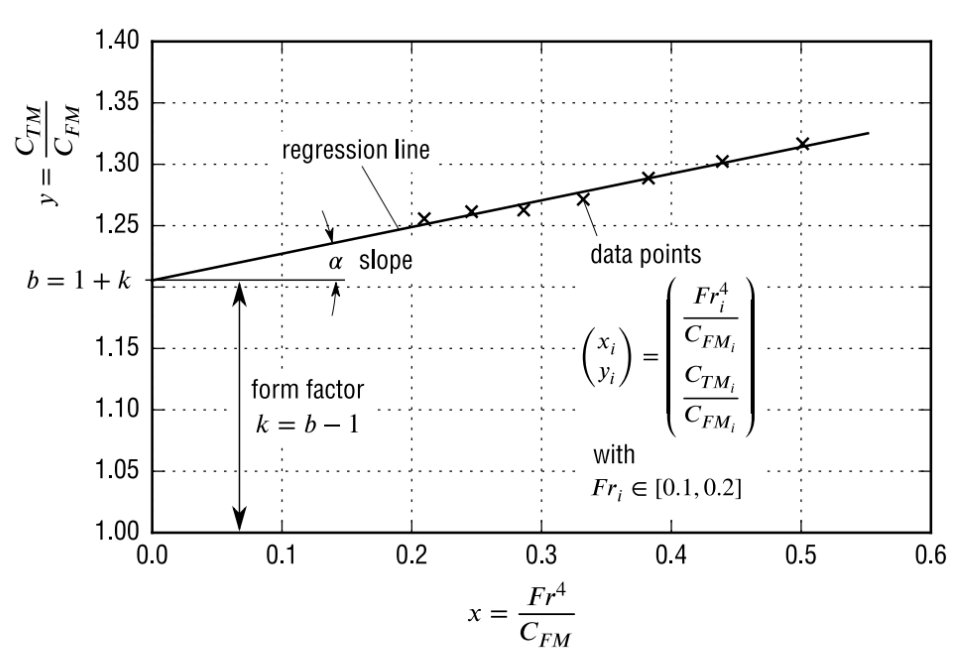
\includegraphics[width=0.65\textwidth]{images/prohaska_diagram}
    \caption{Diagrama del método de Prohaska. Adaptado de \citet{birk2019}.}
    \label{fig:prohaska_esquema}
\end{figure}

El método presenta, sin embargo, limitaciones bien documentadas. La sensibilidad del método a pequeñas incertidumbres de medición es elevada precisamente donde la señal de fuerza es más baja. Las fuentes de desviación pueden agruparse en tres categorías.

La primera corresponde a efectos geométricos no lineales. La presencia de proas bulbo (protuberancias redondeadas ubicadas en la parte sumergida de la proa, concebidas para generar un sistema de olas que interfiere con el del casco y reduce la resistencia por generación de olas) próximas a la superficie libre genera no linealidades en la curva a bajas velocidades que dificultan la extrapolación \citep{korkmaz_cfd_2021}. En \citet{korkmaz_cfd_2021} se analizaron dos modelos con geometrías casi idénticas (95\% de similitud) que mostraron comportamientos divergentes en la determinación del factor de forma mediante el método de Prohaska. Como se observa en la Figura~\ref{fig:korkmaz_bulb_effect}, el primer modelo (Hull-1) presentó una marcada concavidad en la gráfica de $C_T/C_{F0}$ frente a $Fr^n/C_{F0}$ dentro del rango $0.1 < Fr < 0.2$, mientras que el segundo (Hull-2) mantuvo una tendencia lineal. Esta anomalía en el primer caso se atribuyó a un diseño de bulbo tipo ``goose-neck'' con mayor concentración de volumen cerca de la superficie libre, lo cual genera sistemas de ondas cortos que no interactúan favorablemente con el tren de ondas de la proa a bajas velocidades. Este fenómeno se intensificó al ensayar el modelo en condición de lastre, donde la proximidad del bulbo a la superficie libre indujo una protuberancia significativa en la curva, dificultando la extrapolación precisa de la resistencia viscosa.

La segunda fuente de desviación proviene de fenómenos viscosos asociados a la separación del flujo. Cualquier aparición de separación o desprendimiento de vórtices a baja velocidad contradice el supuesto fundamental del método, que presupone un flujo adherido en la condición de referencia. Los cascos con formas llenas pueden presentar pequeñas zonas de separación en la popa o bajo el espejo, especialmente cuando existen apéndices. Las observaciones originales de Prohaska sobre curvas convexas en buques de doble hélice responden a este tipo de efectos: los soportes, ejes o popas voluminosas generaban una resistencia adicional por presión (resistencia por vórtices) incluso a bajos $Fr$, resultando en valores de $C_T$ superiores a los esperados por fricción pura. De manera similar, la separación de flujo en popas espejo sumergidas genera no linealidades \citep{keh-sik-min, korkmaz_cfd_2021}. Una popa espejo parcialmente sumergida puede inducir separación en la estela a escala modelo, fenómeno que no necesariamente se reproduce a escala buque debido a diferencias en el número de Reynolds. Estos efectos, esencialmente viscosos, se traducen en un ``abultamiento'' en la curva de Prohaska por la aparición de un componente adicional de resistencia de forma. Prohaska advirtió que su método no debía aplicarse de forma automática cuando existe separación de flujo, señalando la dificultad de detectar estos fenómenos (por ejemplo, el desprendimiento en popas espejo o zonas de spray separadas en bulbos apenas aflorantes). Estudios más recientes de CFD \citep{korkmaz-verif-and-valid-cfd-efd} confirman que separaciones leves pueden provocar una disminución aparente del factor de forma al aumentar el número de Reynolds, dado que el flujo tiende a re-adherirse progresivamente a mayor velocidad.

La tercera fuente de desviación es de naturaleza analítica y se desdobla, a su vez, en dos aportes. Por un lado, la línea de referencia interviene en el denominador del diagrama: con la ITTC-57, cuya pendiente a bajos $Re$ ya se discutió en la Sección~\ref{sec:ITTC57}, los puntos adquieren una curvatura convexa que no responde al comportamiento del casco \citep{ITTC_Combined_2021}. Por otro, la propia formulación de Prohaska supone que la resistencia por olas varía como ${\sim}Fr^4$; si la ley real difiere de esa potencia --por ejemplo, por la presencia de un sistema secundario de ondas-- los puntos experimentales se apartan de la linealidad esperada, con independencia de la línea de fricción empleada.

% ---------------------------------------------------------------------
% [CORREGIDO] Se explicita cuáles de las tres fuentes intervienen en los
% cascos de esta tesis y dónde se aborda cada una.
% ---------------------------------------------------------------------
Las tres fuentes intervienen simultáneamente en los pesqueros de baja esbeltez
analizados en esta tesis, y su tratamiento organiza buena parte del
Capítulo~\ref{cap:resistencia_factor_de_forma}: la primera a través de la proa
bulbo, cuyo efecto sobre el diagrama de Prohaska se aísla comparando el casco
original con una variante sin bulbo (Sección~\ref{sec:proa_bulbo}); la segunda a
través de la popa espejo, que en la condición de plena carga queda
sustancialmente sumergida y genera separación (Sección~\ref{sec:popa_sumergida});
y la tercera a través de la sensibilidad del valor de $(1+k)$ al rango de Froude
retenido en la regresión. Una primera cuantificación conjunta de estos efectos
para esta clase de cascos se presentó en \citet{oyuela2024jmse}.

\begin{figure}[htbp]
    \centering
    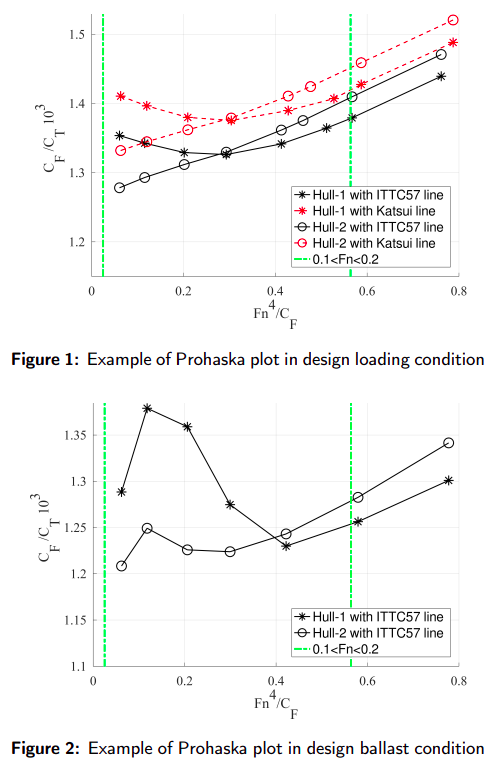
\includegraphics[width=0.6\textwidth]{images/prohaska-korkmaz.png}
    \caption{Diagramas de Prohaska de los modelos Hull-1 y Hull-2. Adaptado de
    \citet{korkmaz_cfd_2021}.}
    \label{fig:korkmaz_bulb_effect}
\end{figure}

\section{Determinación del factor de forma asistida por CFD}
\label{sec:cfd_ff_antec}

El recurso al CFD para determinar el factor de forma plantea dos cuestiones
independientes, que se corresponden con los dos miembros del cociente
$(1+k) = C_V/C_{F0}$ de la Ecuación~\eqref{eq:k_dos_cocientes}. La primera es
cómo obtener el numerador, es decir por qué camino se llega a la resistencia
viscosa $C_V$. Hay dos posibles: reproducir numéricamente el ensayo de remolque
--con superficie libre, sobre el mismo rango de bajos $Fr$ que la campaña
experimental-- y aplicar sobre los resultados el método de Prohaska igual que
sobre datos medidos, o bien eliminar la superficie libre del problema y calcular
$C_V$ de forma directa, que es el enfoque de doble cuerpo. La segunda cuestión es
cuál adoptar como denominador: la línea de fricción de referencia $C_{F0}$ deja
de ser un dato heredado de la práctica experimental y pasa a poder calcularse con
el mismo código y el mismo modelo de turbulencia que se emplean para el casco.
Ambas cuestiones se tratan a continuación por separado.

\subsection{Líneas de fricción numéricas}
\label{sec:nfl_antec}

Cualquiera sea la vía por la que se obtenga $C_V$, el cociente $C_V/C_{F0}$ que
define el factor de forma queda referido a una línea de fricción de origen
distinto al del numerador: $C_V$ sale de una simulación y $C_{F0}$, si se adopta
la ITTC-57, de una correlación experimental que además embebe un factor de forma.
Para evitar esa inconsistencia se han derivado diversas \textbf{líneas de fricción numéricas}
(``Numerical Friction Lines'', NFL) mediante simulaciones CFD de placa plana a
distintos Reynolds \citep{wang2015numericalFL, Korkmaz2019NumericalFL}. A
diferencia de la ITTC-57, no incorporan ningún margen de correlación: son
fricción de placa plana pura, calculada con el mismo código y el mismo modelo de
turbulencia que luego se emplea para el casco. Las
diferencias entre formulaciones se concentran en el rango de números de Reynolds
propio de los modelos de laboratorio y se atenúan marcadamente hacia la escala
buque. La Figura~\ref{fig:lineas_friccion} compara el coeficiente de fricción
$C_F$ de varias de estas líneas (la NFL $k$--$\omega$ SST de
\citet{wang2015numericalFL}, la NFL $k$--$\omega$ SST de \citet{eca2008friction}
y la NFL con el modelo EASM de \citet{Korkmaz2019NumericalFL}) tomando como
referencia la línea ITTC-57. Se observa que todas las líneas numéricas predicen
valores de $C_F$ inferiores a los de la ITTC-57 en el rango de bajos $Re$. Las
distintas NFL $k$--$\omega$ SST coinciden entre sí dentro de un margen del orden
del $2\%$, mientras que la formulación EASM se aparta ligeramente, evidenciando
la influencia del modelo de turbulencia empleado en la derivación
\citep{korkmaz2023thesis}. Hacia el régimen de escala buque las diferencias
entre todas las formulaciones se reducen de manera considerable.

\begin{figure}[htpb]
    \centering
    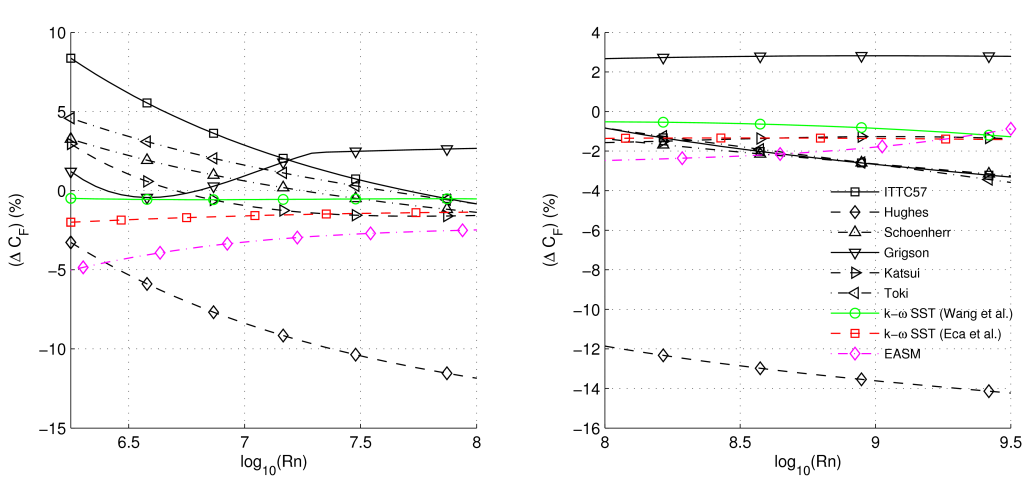
\includegraphics[width=0.7\textwidth]{images/comparacion_lineas_friccion.png}
    \caption{Líneas de fricción numéricas frente a la línea ITTC-57. Adaptado de
    \citet{korkmaz2023thesis}.}
    \label{fig:lineas_friccion}
\end{figure}

En esta tesis las NFL no reemplazan a la línea de referencia adoptada, sino que
se emplean como herramienta de diagnóstico: comparar el factor de forma obtenido
con una y con otra permite separar lo que en su comportamiento con la escala es
atribuible a la línea de referencia de lo que responde a la física del flujo
(Sección~\ref{sec:k_vs_Re}).

\subsection{El enfoque de doble cuerpo}
\label{sec:doble_cuerpo_antec}

% ---------------------------------------------------------------------
% [CORREGIDO] La analogía se establece con el MÉTODO DE BAJAS VELOCIDADES
% (que sí supone C_W despreciable), no con la descomposición de Hughes.
% ---------------------------------------------------------------------
El enfoque de doble cuerpo persigue el mismo objetivo que el método de Prohaska
--acceder a la resistencia viscosa sin la contaminación de la componente por
olas-- pero lo alcanza por una vía que no es equivalente en rigor. Prohaska lo
hace de forma indirecta: supone para $C_W$ una ley de potencia en $Fr$ y la
sustrae por extrapolación, de modo que el valor obtenido depende del rango de
velocidades retenido y de que la ley supuesta describa bien el tren de olas real.
La configuración de doble cuerpo, en cambio, elimina la generación de olas por
construcción, al reemplazar la superficie libre por un plano de simetría: allí
$C_W = 0$ de manera exacta, y no por aproximación ni por sustracción. Esto libera
además al método de toda restricción sobre el número de Froude, ya que puede
computarse cualquier velocidad --y, de hecho, cualquier número de Reynolds,
incluido el del buque-- con la única condición de que el flujo sea turbulento.

Formalmente, al anularse la generación de olas, la resistencia
total obtenida en esta configuración corresponde únicamente a la componente
viscosa, y el factor de forma se obtiene como \citep{ITTC_Combined_2021}:
%
\begin{equation}
    (1+k) = \frac{C_V}{C_{F0}} = \frac{C_F + C_{PV}}{C_{F0}},
\end{equation}
%
donde $C_V = C_F + C_{PV}$ es el coeficiente de resistencia viscosa obtenido de la simulación de doble cuerpo y $C_{F0}$ el coeficiente de la línea de referencia. La ventaja decisiva sobre el método de Prohaska es que el doble cuerpo elimina la contaminación por olas en la determinación de $C_V$ (la mayor fuente de incertidumbre de Prohaska a bajas velocidades) en lugar de intentar sustraerla por extrapolación. La configuración permite además concentrar la resolución de la malla en la capa límite y la estela viscosa de popa, optimizando el costo computacional frente a las simulaciones con superficie libre. Cabe señalar, sin embargo, que la condición de simetría impuesta en la frontera superior puede distorsionar el campo de presiones en la zona de la proa bulbo cuando esta se encuentra próxima a la superficie libre, por lo que su aplicación requiere verificar que la geometría simulada no se vea afectada por esta limitación. En efecto, en \citet{quintuna2023} se observó que, cuando existe un pequeño espacio entre el tope del bulbo y la superficie libre en reposo, la tapa rígida induce una separación de flujo en torno al bulbo que no se produce en las simulaciones con superficie libre, y que este efecto se atenúa al aumentar la inmersión de la proa mediante el asiento, en línea con lo señalado en \citet{korkmaz_cfd_2021}.

\subsection{Resultados disponibles: de los cascos de referencia a los pesqueros de baja esbeltez}
\label{sec:estado_arte_ff}

El Comité Especialista de la 29a ITTC sobre Métodos Combinados CFD/EFD coordinó un
estudio colaborativo en el que nueve organizaciones y ocho códigos calcularon el
factor de forma para los cascos \textit{KCS} y KVLCC2 \citep{ITTC_Combined_2021,
KORKMAZ2022112590}. Los resultados mostraron que la dispersión entre
organizaciones es significativamente menor que la del método de Prohaska, que el
valor medio de las predicciones CFD concuerda con el experimental dentro de la
incertidumbre, y que las predicciones de potencia a escala buque mejoran de manera
generalizada al utilizar factores de forma basados en CFD. Con base en estos
resultados, la ITTC recomienda el uso del CFD como complemento al método
experimental.

Esa evidencia proviene, sin embargo, de cascos de esbeltez moderada. Para cascos
pesqueros con $L/B < 4$ el punto de partida es \citet{oyuela2024jmse}, donde se
determinó el factor de forma de un pesquero por el método de doble cuerpo y se lo
contrastó con el obtenido experimentalmente sobre el mismo casco en el LabHiNO
(Laboratorio de Hidrodinámica Naval y Oceánica, UBA), verificando que el CFD
reproduce el valor medido. Trabajos posteriores del mismo grupo ampliaron el
análisis a la influencia del modelo de turbulencia \citep{oyuela2025mecanica} y a
la comparación con el \textit{KCS} \citep{oyuela2026oceaneng}, que permite situar
el comportamiento de estos cascos frente al de una geometría de referencia.

La ventaja del doble cuerpo frente a Prohaska en esta clase de buques no reside en
una mayor exactitud intrínseca, sino en que suprime la principal fuente de
ambigüedad del método experimental: al no requerir extrapolación desde el rango de
bajos $Fr$, el valor de $(1+k)$ deja de depender de qué puntos se retienen en la
regresión, dependencia que resulta particularmente marcada cuando el espejo de
popa está sustancialmente sumergido. La contrapartida es que la configuración de
doble cuerpo introduce su propia idealización en esa misma zona --la tapa rígida
impone un plano de simetría allí donde el espejo interrumpe la superficie libre--,
de modo que ambos métodos deben leerse como complementarios y no como sustitutos.
Esta comparación se retoma, con los resultados propios, en el
Capítulo~\ref{cap:resistencia_factor_de_forma}.

\section{Dependencia del factor de forma con el número de Reynolds}
\label{sec:k_vs_Re}

Presentado el método completo y sus variantes de determinación, corresponde
examinar el único supuesto que no puede contrastarse dentro del propio ensayo:
que el factor de forma determinado sobre el modelo es el mismo que gobierna el
flujo alrededor del buque, $k_M = k_S$. La evidencia acumulada en las últimas
décadas indica que el factor de forma \emph{aparente} --el que resulta de
aplicar los procedimientos descritos con la línea ITTC-57-- no es constante,
sino que crece de manera sistemática con el número de Reynolds, de modo que
$k_M < k_S$.

Conviene precisar dónde se introduce el error que esto acarrea. El valor
determinado sobre el modelo es el correcto para despejar $C_W$ del ensayo, porque
$k_M$ es justamente el factor de forma que gobierna el flujo a esa escala; el
término de olas se traslada entonces al buque sin error. La discrepancia aparece
recién al recomponer el coeficiente del buque, donde la
Ecuación~\eqref{eq:extrapolacion_CTS} emplea $(1+k_M)$ allí donde correspondería
$(1+k_S)$. La diferencia entre la predicción correcta y la estándar vale
$(k_S - k_M)\,C_{F0}(Re_S)$, positiva siempre que $k_S > k_M$: el término viscoso
de escala buque queda subestimado, y con él la resistencia total del buque.

Dos mecanismos independientes explican por qué cabe esperar esta dependencia.
El primero es físico: el flujo en el modelo está necesariamente a menor número
de Reynolds que en el buque, lo que implica que la capa límite es
proporcionalmente más gruesa, el gradiente de presión adverso en la popa está
más amortiguado y la posible zona de separación es más extensa en el modelo que
en el buque. El segundo es metodológico y remite a las propiedades de la línea de
referencia descritas en la Sección~\ref{sec:ITTC57}, que introducen una
distorsión sistemática en el valor de $k$ calculado con ella. Ambos efectos
actúan en el mismo sentido, $k_M < k_S$.

La cuantificación sistemática de este efecto fue abordada por primera vez en
\citet{gomezgarcia}, donde se reanalizaron quince modelos agrupados en cuatro
familias de modelos geométricamente semejantes a distinta escala. Para cada
familia, el factor de forma determinado por Prohaska con la ITTC-57 disminuye al
aumentar la razón de escala $\lambda$ --equivalentemente, crece con el tamaño
del modelo--, de modo que la extrapolación de la recta de regresión a
$\lambda = 1$ predice un factor de forma de buque mayor que el de cualquier
modelo. El efecto de escala resultante, $k_S - k_M$, crece linealmente con
$\lambda$ (Figura~\ref{fig:gomez-garcia}). Forzando la recta por su valor
teórico en el origen ($k_S - k_M = 0$ para $\lambda = 1$), en
\citet{gomezgarcia} se propone la forma práctica
%
\begin{equation}
    k_S - k_M = 1.91\,(\lambda - 1)\times 10^{-3},
    \label{eq:gomezgarcia}
\end{equation}
%
positiva para todo modelo ($\lambda > 1$), lo que confirma $k_M < k_S$. Con la
línea de Schoenherr (otra línea de fricción de placa plana disponible como
referencia, alternativa a la ITTC-57) la pendiente resulta significativamente
menor, dado que sus coeficientes de fricción a $Re$ de modelo son más próximos a
los de escala buque que los de la ITTC-57: un primer indicio de que parte del
efecto no es físico sino atribuible a la referencia elegida. En
\citet{ITTC_Combined_2021} se estimó que una extrapolación estándar con factor
de forma constante puede subestimar la resistencia del buque en hasta un 10\%.

\begin{figure}[htpb]
\centering
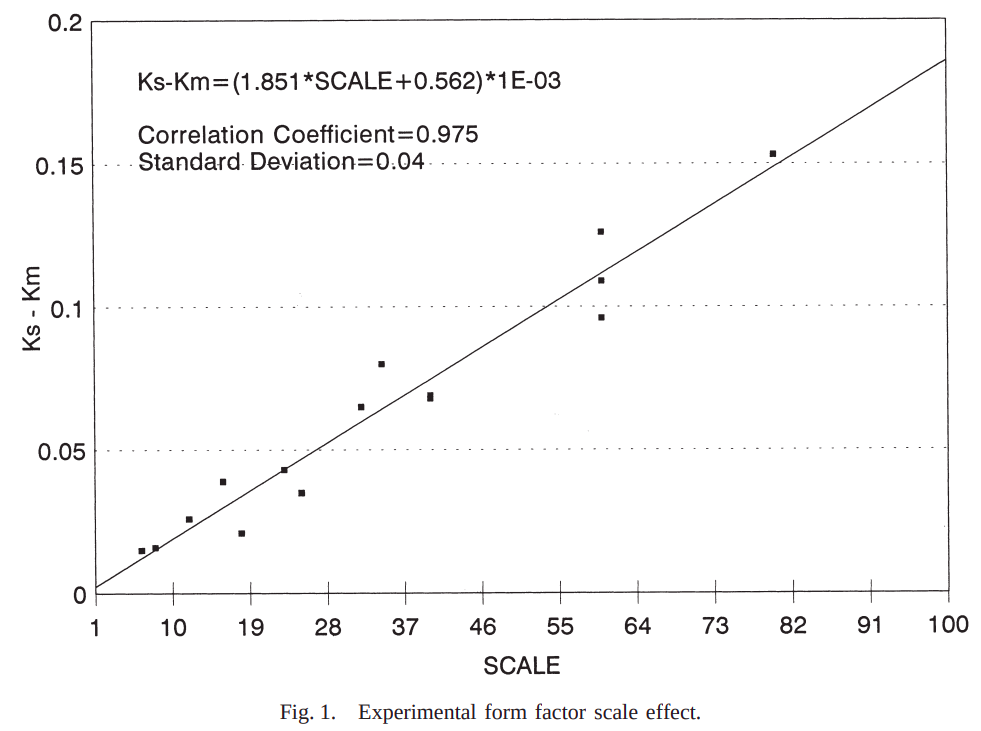
\includegraphics[width=0.6\textwidth]{images/gomez-garcia.png}
\caption{Efecto de escala del factor de forma en función de la razón de escala.
Adaptado de \citet{gomezgarcia}.}
\label{fig:gomez-garcia}
\end{figure}

Un programa experimental de alcance comparable, extendido entre 1992 y 2006, se
presenta en \citet{keh-sik-min}: doce buques de distinto tipo ensayados sobre un
total de 32 modelos, construidos en varias escalas para un mismo casco de modo
de barrer el número de Reynolds manteniendo el de Froude. La Figura~\ref{fig:keh-sik} reproduce los resultados de los ensayos de baja
velocidad para los cuatro modelos geosim de un portacontenedores de 8600~TEU,
graficados como $C_{TM}/C_{FM}$ frente a $Fr$. En ese plano, el valor al que
tiende cada curva cuando $Fr \to 0$ es el factor de forma, según la definición
adoptada por la ITTC en 1978 y empleada por los autores. Dos rasgos son
relevantes. El primero es que ese valor asintótico crece de manera sistemática
con la eslora del modelo --y por lo tanto con $Re$--: aplicando su procedimiento
estándar, los autores obtienen $1.008$ y $1.012$ en los modelos de 2 y 4~m frente
a $1.102$ y $1.124$ en los de 7.6 y 10~m para un mismo buque. El segundo es que
las curvas de los dos modelos pequeños son cualitativamente distintas de las de
los grandes: presentan una caída pronunciada y un quiebre por debajo de
$Fr \approx 0.06$ que las curvas de los modelos mayores no exhiben. Los propios autores atribuyen ese comportamiento a
que, con números de Reynolds del orden de $10^5$, el flujo alrededor de los
modelos pequeños es mayormente laminar o transicional.

\begin{figure}[htbp]
\centering
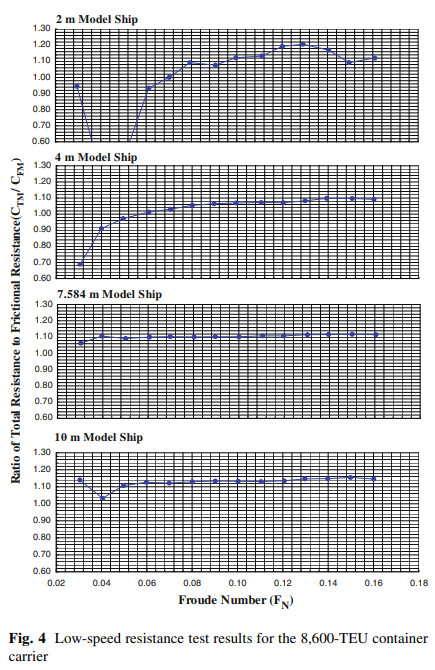
\includegraphics[width=0.6\textwidth]{images/keh-sik-min.png}
\caption{Ensayos de baja velocidad de los cuatro modelos geosim del
portacontenedores de 8600~TEU. Adaptado de \citet{keh-sik-min}.}
\label{fig:keh-sik}
\end{figure}

Sobre esta base, en \citet{keh-sik-min} se propone un \textbf{factor de forma
terminal}, definido como el valor al que tiende $(1+k)$ cuando el flujo alcanza
el régimen plenamente turbulento --que los autores sitúan en $Re \sim 10^9$, y
que en la práctica corresponde al buque a velocidad de diseño--, y un
\textbf{factor de corrección} que permite llevar el valor medido en la escala de
ensayo hasta ese valor terminal. La curva de corrección, ajustada por una
función tangente hiperbólica del logaritmo de $Re$, se muestra en la
Figura~\ref{fig:keh-sik-2}.

Conviene señalar una limitación de esta evidencia, que condiciona la
interpretación tanto de la Figura~\ref{fig:keh-sik} como de la propia curva de
corrección: en esa campaña no se emplearon estimuladores de turbulencia en
ninguno de los modelos. Parte del crecimiento observado de $(1+k)$ con el tamaño
del modelo no responde entonces a una dependencia física del factor de forma con
$Re$, sino a que los modelos pequeños no alcanzan el régimen turbulento sobre el
que la hipótesis de Hughes está formulada. Los propios autores son consistentes
con esta lectura: sostienen que, una vez plenamente turbulento el flujo, el
factor de forma se estabiliza en su valor terminal. Lo que la evidencia
establece con solidez, por lo tanto, no es que $k$ varíe intrínsecamente con el
número de Reynolds, sino algo suficiente para el problema que aquí interesa: que
el valor medido a escala de modelo no es, sin corrección, el valor que gobierna
el flujo alrededor del buque.

\begin{figure}[h]
\centering
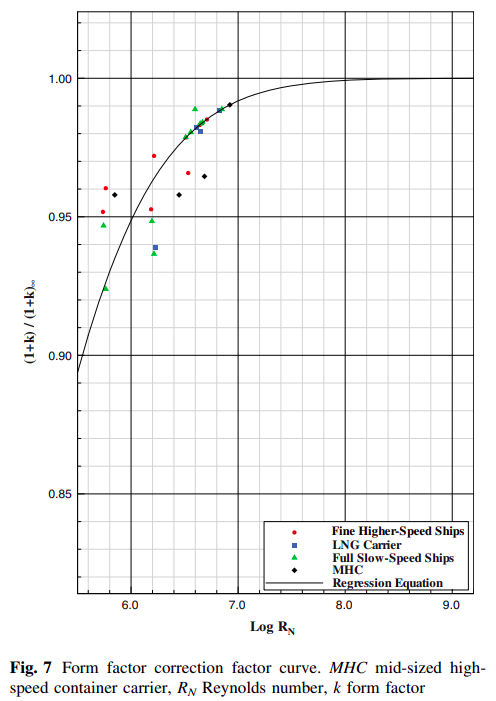
\includegraphics[width=0.6\textwidth]{images/keh-sik-min-2.png}
\caption{Curva del factor de corrección del factor de forma. Adaptado de
\citet{keh-sik-min}.}
\label{fig:keh-sik-2}
\end{figure}

La pregunta clave es en qué medida esta dependencia con $Re$ es un artefacto de la línea de referencia y en qué medida refleja física real. La evidencia acumulada permite separar tres contribuciones distintas. A ellas se agrega, por último, una configuración geométrica particular en la que la segunda de esas contribuciones se vuelve dominante y exige un tratamiento propio.

\subsection{La contribución de la línea de referencia}

El estudio colaborativo ITTC \citep{korkmaz_cfd_2021} aportó evidencia concluyente: la dependencia de $k$ con
$Re$ desaparece casi por completo al reemplazar la ITTC-57 por líneas de
fricción numéricas derivadas con el mismo código, al menos para cascos de
esbeltez moderada como el \textit{KCS} y el KVLCC2. Esto indica que la mayor
parte de la dependencia observada es un artefacto de la pendiente incorrecta de
la ITTC-57 a bajos números de Reynolds, y no un efecto físico inherente. En la
misma dirección, en \citet{quintuna2023} se determinaron factores de forma por
CFD de doble cuerpo para un buque multipropósito y un portacontenedores, y se
cuantificó que la diferencia del factor de forma entre escala modelo y escala
buque se reduce en promedio del $10.4\%$, al emplear la línea ITTC-57, al
$6.4\%$ al utilizar una NFL derivada con el modelo $k$--$\omega$ SST.

Estas cifras admiten, sin embargo, una segunda lectura: la reducción es
sustancial pero no completa, y la fracción remanente no puede atribuirse a la
referencia. En efecto, la mejora no es universal. En configuraciones con
apéndices, o en cascos donde la resistencia por presión viscosa $C_{PV}$
constituye una fracción significativa de la resistencia viscosa total, el factor
de forma continúa mostrando variaciones apreciables con el número de Reynolds
incluso al emplear NFL, lo que indica que la hipótesis de proporcionalidad entre
resistencia viscosa y fricción de placa plana resulta insuficiente en flujos
tridimensionales complejos \citep{wang2015numericalFL}. Este es precisamente el
caso de los pesqueros de baja esbeltez analizados en esta tesis, como se
documenta en el Capítulo~\ref{cap:resistencia_factor_de_forma}.

\subsection{La contribución física asociada a la forma del casco}

% ---------------------------------------------------------------------
% [REESCRITO] Sin referencia al método de Froude: todo el argumento se
% expresa dentro de la descomposición de Hughes.
% ---------------------------------------------------------------------
La contribución analizada en el apartado anterior afecta al primer término de la
Ecuación~\eqref{eq:k_dos_cocientes}: una línea de referencia con pendiente
incorrecta hace que $C_F/C_{F0}$ varíe con $Re$ aun cuando la física del casco
sea la esperada. El segundo término, en cambio, no se corrige cambiando la
referencia. Sostener $k_M = k_S$ exige también que la resistencia por presión
viscosa $C_{PV}$ mantenga una proporción invariante al aumentar el número de
Reynolds, y es ahí donde interviene la forma del casco.

En \citet{DOGRUL2020107428} se calcularon por CFD de doble cuerpo los factores
de forma del \textit{KCS} y del KVLCC2 en tres escalas de modelo y en escala
real, empleando como referencia tanto la línea ITTC-57 como la ATTC-1947. El
resultado directo es que $(1+k)$ crece de manera monótona con $Re$ en ambos
cascos: con la ITTC-57, aproximadamente de $1.10$ a $1.16$ en el \textit{KCS} y
de $1.20$ a $1.27$ en el KVLCC2 entre el modelo más pequeño y la escala buque. La
comparación entre ambas líneas de referencia reproduce, de paso, el
comportamiento descrito en el apartado anterior: las diferencias entre los
valores obtenidos con una y otra son apreciables en el rango de Reynolds de
modelo y se anulan en escala buque, donde las dos líneas de fricción convergen.

Las simulaciones con superficie libre del mismo trabajo permiten ubicar ese
crecimiento en el segundo término de la Ecuación~\eqref{eq:k_dos_cocientes}. Por
un lado, el coeficiente de fricción calculado sobre el casco se aproxima
estrechamente a la línea ITTC-57 en todas las escalas, de modo que el cociente
$C_F/C_{F0}$ no aporta una variación apreciable. Por otro, la resistencia por
presión viscosa disminuye de manera sistemática con $Re$ en ambos cascos, en
correspondencia con una recuperación de presión más completa en la popa a medida
que la capa límite se adelgaza. El efecto neto es que $C_{PV}$ decrece, pero más
lentamente que la fricción de referencia, y el cociente $C_{PV}/C_{F0}$ --es
decir, el factor de forma-- crece con la escala.

La forma del casco no interviene en el signo de este efecto, que es el mismo en
ambos buques, sino en el peso que el segundo término tiene sobre el total. La
presión viscosa representa alrededor del $7\%$ de la resistencia total del
\textit{KCS} en todas las escalas, frente a un $16$--$17\%$ en el KVLCC2, de
formas mucho más llenas; los factores de forma correspondientes son también
mayores en este último. Cuanto mayor es esa fracción, mayor es la porción de
$(1+k)$ que queda gobernada por un término que no escala como la fricción, y
menos margen hay para tratar el factor de forma como una constante puramente
geométrica. Los cascos pesqueros de muy baja esbeltez analizados en esta tesis se
ubican en el extremo de esa tendencia, y es ésta la razón por la cual corregir la
línea de referencia no basta para estabilizar su factor de forma, como se
documenta en el Capítulo~\ref{cap:resistencia_factor_de_forma}.

\subsection{El comportamiento a muy bajos números de Froude}

En \citet{TERZIEV2021147} se abordó esta cuestión numéricamente, calculando por
doble cuerpo el factor de forma de una serie geosim del \textit{KCS} sobre cuatro
factores de escala ($\lambda = 75$, $52.667$, $31.599$ y $1$), catorce números de
Froude entre $0.02$ y $0.28$ y tres modelos de turbulencia ($k$-$\omega$,
$k$-$\varepsilon$ y $k$-$\omega$ SST). El estudio se complementó con simulaciones
de escalado viscoso, en las que el número de Reynolds se altera modificando la
viscosidad del fluido a Froude fijo, lo que permite separar ambos efectos de un
modo inaccesible experimentalmente.

El trabajo reporta, en efecto, una dependencia con el número de Froude, pero
acotada en su alcance. La variación se concentra en el rango $Fr = 0.02$--$0.06$,
donde las diferencias entre velocidades adyacentes alcanzan el $10$--$20\%$, con
un máximo del $20.9\%$; por encima de ese rango caen por debajo del $1\%$, y el
escalado viscoso no detecta efecto alguno entre $Fr = 0.26$ y $0.28$.

Los propios autores matizan además ese hallazgo. La incertidumbre numérica se
mantiene por debajo del $2\%$ en la mayoría de los casos, pero los valores
atípicos por encima del $5\%$ provienen exclusivamente de ese mismo extremo
inferior, lo que indica que el método RANS se ve más exigido allí que a
velocidades intermedias o altas. Y la dispersión entre modelos de turbulencia
resulta mayor que la atribuible al Froude: a $\lambda = 75$ y $Fr = 0.02$ el
factor de forma pasa de $1.029$ con el modelo SST a $1.185$ con el
$k$-$\varepsilon$, una diferencia que excede las bandas de incertidumbre de ambos.
Señalan que ello dificulta sostener argumentos concretos en esa región, y cierran
indicando que la naturaleza del efecto de escala sobre el factor de forma, tanto
en Froude como en Reynolds, requiere investigación adicional. Para lo que aquí
interesa, la consecuencia es que el rango en el que la variación se manifiesta
queda por debajo de la ventana $Fr \in [0.1;\, 0.2]$ sobre la que opera el método
de Prohaska, dentro de la cual las diferencias reportadas son de unos pocos por
ciento.
\subsection{Una configuración particular: la popa espejo sumergida}

Cuando la popa del casco tiene el espejo sumergido, el flujo se separa en la arista y se forma detrás una zona de recirculación persistente. La inmersión del espejo se acentúa al aumentar el calado y al reducir la velocidad, de modo que el régimen recirculante es más probable en condición de plena carga y, dentro de ella, justamente en el rango de bajos $Fr$ sobre el que operan los métodos de determinación de $(1+k)$. En esa configuración, el flujo de escala modelo y el flujo de escala buque difieren cualitativamente, no solo cuantitativamente, porque la velocidad crítica a la que el espejo ``ventila'' y pasa a flujo libre es diferente en las dos escalas \citep{ITTC_Combined_2021}. Para este caso, en \citet{korkmaz_wetted_transom} se propone un \textbf{método de dos factores de forma} ($2k$) que distingue la contribución del cuerpo sin separación de la contribución adicional de la popa espejo, calculando ambas por CFD en escala modelo y buque respectivamente. El método incluye un criterio de aplicabilidad basado en el área sumergida del espejo relativa a la sección maestra. Los cascos pesqueros analizados en esta tesis superan ese umbral en su condición de plena carga, de modo que la corrección corresponde ser aplicada; cuánto explica del efecto de escala medido en ellos es una cuestión distinta, que se cuantifica en la Sección~\ref{sec:popa_sumergida}.

Recientemente en \citet{starke2025} se propuso una variante en la que el factor de forma se calcula sobre una versión del casco con la popa geométricamente cerrada, dejando la resistencia de la popa espejo fuera del escalado viscoso (verificada sobre diez cascos, reduce la subestimación de la resistencia a escala buque a un $0$--$3\%$). Su comparación sistemática con el método de dos factores de forma para los cascos aquí estudiados queda como línea de trabajo futuro.
 
 
\section{Hidrodinámica de hélices en aguas abiertas}
\label{sec:helices_antec}
 
\subsection{Coeficientes adimensionales y ensayo en aguas abiertas}
\label{sec:pow_antec}
 
El comportamiento hidrodinámico de una hélice se caracteriza a través de su \textbf{diagrama de aguas abiertas} (``Propeller Open Water diagram'', POW), obtenido en ensayos donde la hélice opera en flujo uniforme sin influencia del casco. Las variables de interés son el coeficiente de empuje $K_T$, el coeficiente de par $K_Q$ y la eficiencia en aguas abiertas $\eta_0$:
%
\begin{equation}
    K_T = \frac{T}{\rho n^2 D^4}, \qquad
    K_Q = \frac{Q}{\rho n^2 D^5}, \qquad
    \eta_0 = \frac{K_T}{K_Q}\,\frac{J}{2\pi},
\end{equation}
%
donde $T$ es el empuje, $Q$ el par, $\rho$ la densidad del fluido, $n$ la velocidad de giro en rev/s, $D$ el diámetro y $J = V_a/(nD)$ el coeficiente de avance, con $V_a$ la velocidad de avance del flujo incidente. Se denota $R = D/2$ el radio de la pala y $r$ la coordenada radial medida desde el eje, de modo que $r/R$ es la posición radial adimensional que identifica cada sección de la pala.

La caracterización del régimen de flujo sobre la pala admite dos números de Reynolds de uso corriente, que conviene distinguir explícitamente porque no son intercambiables. El primero es el \textbf{número de Reynolds rotacional},
%
\begin{equation} \label{eq:Re_rotacional}
    Re_n = \frac{n D^2}{\nu},
\end{equation}
%
construido únicamente con parámetros globales de operación y empleado para identificar el punto de funcionamiento de una campaña completa. El segundo es el \textbf{número de Reynolds seccional}, definido sobre una sección concreta de la pala. Para la sección ubicada en la posición radial $r/R$ se denota $c_{r/R}$ la longitud de su cuerda, es decir la distancia entre el borde de ataque y el borde de salida del perfil que resulta de cortar la pala a ese radio, que es la dimensión característica sobre la que se desarrolla la capa límite en esa sección:
%
\begin{equation} \label{eq:Re_helice}
    Re_c = \frac{c_{r/R}\, V_{r/R}}{\nu}, \qquad V_{r/R} = \sqrt{V_a^2 + \left(\pi n D\, \tfrac{r}{R}\right)^2},
\end{equation}
%
donde $V_{r/R}$ es la velocidad resultante del flujo incidente sobre esa sección, compuesta por la velocidad de avance y la velocidad tangencial de rotación. Este último es el que gobierna el estado de la capa límite sobre la pala y, por lo tanto, el que aparece en los criterios de representatividad de los ensayos y en el procedimiento de extrapolación. Dado que la sección de referencia no es la misma en todos los procedimientos --la ITTC evalúa la representatividad del ensayo de aguas abiertas a $r/R = 0.7$ y construye la corrección de arrastre del procedimiento ITTC-78 a $r/R = 0.75$--, se indica en cada caso la sección empleada mediante la notación $Re_{c,0.7R}$ y $Re_{c,0.75R}$ \citep{ITTC_Performance_prediction}.
 
\subsection{La serie Wageningen B}
\label{sec:wageningen_antec}
 
La \textbf{serie Wageningen B} es la familia sistemática de hélices de referencia más ampliamente utilizada en la industria naval. Comprende modelos experimentados en el canal MARIN cubriendo de $Z = 2$ a $Z = 7$ palas, relaciones de área expandida $A_E/A_0$ de $0.30$ a $1.05$ (cociente entre el área expandida de las palas y el área del disco de la hélice) y relaciones paso--diámetro $P/D$ de $0.5$ a $1.4$ (con $P$ el paso geométrico y $D$ el diámetro de la hélice). Los resultados originales de \citet{troost1940} fueron corregidos por efectos de escala y ajustados a polinomios de regresión en \citet{oosterveld1975}, cuyas expresiones para $K_T$ y $K_Q$ en función de $J$, $P/D$, $A_E/A_0$ y $Z$ son actualmente la referencia estándar. Dichos polinomios fueron obtenidos a $Re_{c,0.75R} = 2\times10^6$ y son la base para la hélice B4-60 ($P/D = 0.81$, $D = 0.14$~m) analizada numéricamente en el LabHiNO (Laboratorio de Hidrodinámica Naval y Oceánica, UBA) y presentada en el Capítulo~\ref{chap:helices}. La nomenclatura de la serie identifica, en ese orden, la serie B, el número de palas y la relación de área expandida: B4-60 designa entonces una hélice de cuatro palas con $A_E/A_0 = 0.60$.
 
\section{Efectos de escala en hélices y el procedimiento ITTC-78}
\label{sec:escala_helices}
 
\subsection{El procedimiento ITTC-78 para propulsores}
\label{sec:ittc78_propulsor}
 
El \textbf{procedimiento ITTC-78} extrapola los resultados del ensayo POW de modelo a escala buque asumiendo que toda la diferencia entre escalas es de naturaleza friccional \citep{ITTC_Performance_prediction}. Su único insumo es la corrección del coeficiente de arrastre de perfil de la sección representativa, tomada a $r/R = 0.75$:
%
\begin{equation}
    \Delta C_D = C_{D,M} - C_{D,S},
\end{equation}
%
donde $C_{D,M}$ y $C_{D,S}$ son los coeficientes de arrastre del perfil equivalente en escala modelo y buque, estimados mediante correlaciones de placa plana 2D. El objetivo del método, sin embargo, no es $\Delta C_D$ en sí, sino corregir los coeficientes propulsivos: a partir de esa única diferencia de fricción se calculan las correcciones de empuje y de par, $\Delta K_T$ y $\Delta K_Q$, con las que se ajustan los valores de modelo a escala buque,
%
\begin{equation}
    K_{TS} = K_{TM} - \Delta K_T, \qquad K_{QS} = K_{QM} - \Delta K_Q,
    \label{eq:ittc78_correcciones}
\end{equation}
%
de modo que, siendo $\Delta C_D > 0$, resulta $\Delta K_T < 0$ y $\Delta K_Q > 0$: el empuje aumenta y el par disminuye al pasar de modelo a escala buque. Las expresiones completas de $\Delta K_T$ y $\Delta K_Q$ en función de $\Delta C_D$, junto con las correlaciones de placa plana para $C_{D,M}$ y $C_{D,S}$, se detallan en la Sección~\ref{sec:ittc78_helices_metodo}.
 
Este procedimiento tiene dos limitaciones fundamentales que motivan el trabajo original del Capítulo~\ref{chap:helices}. En primer lugar, ignora los cambios en la distribución de presiones sobre las palas al variar $Re$. En segundo lugar, no contempla el comportamiento no monótono de $K_T$ y $K_Q$ en el rango transicional en el que pueden encontrarse a escala de modelo.
 
\subsection{Insuficiencia de corregir solo fricción: el campo de presiones}
\label{sec:presion_escala}

Al aumentar $Re$ desde escala modelo hacia escala buque, no solo cambia el nivel
de fricción: toda la distribución de presiones sobre la pala se modifica a medida
que la capa límite se adelgaza, la zona de separación en el borde de salida se
reduce y el campo de circulación varía.

En \citet{gallotti2026} se realizó una investigación sistemática por CFD de los
efectos de escala en hélices marinas, definiendo la \textbf{fracción de presión}
$f_p = \Delta K_{Tp}/(\Delta K_{Tp}+\Delta K_{Tf})$ --la porción del incremento de
empuje entre escala de modelo y escala buque atribuible a la componente de
presión-- como métrica cuantitativa del fenómeno. Conviene fijar aquí la
convención de signos, porque difiere de la de la
Ecuación~\eqref{eq:ittc78_correcciones}. En lo que sigue, y en todo el análisis de
efectos de escala del Capítulo~\ref{chap:helices}, $\Delta K_T = K_{TS} - K_{TM}$
denota el \emph{incremento} del coeficiente de empuje al pasar de escala de modelo
($K_{TM}$) a escala buque ($K_{TS}$), cantidad positiva, y se descompone como
$\Delta K_T = \Delta K_{Tp} + \Delta K_{Tf}$ en sus contribuciones de presión y de
fricción, definidas en el Capítulo~\ref{chap:Metodologia}; con esa convención,
$f_p = \Delta K_{Tp}/\Delta K_T$. El procedimiento ITTC-78 adopta en cambio el
signo opuesto, ya que su $\Delta K_T$ es la cantidad que se resta del valor de
modelo para producir ese mismo aumento; al comparar ambos marcos se explicita la
conversión.

El estudio abarca tanto una hélice convencional (VP1304, $A_E/A_0=0.779$, sin
modificación de punta) como una de punta rakeada y área expandida reducida
(P1727, $A_E/A_0=0.444$). El \emph{rake} es el desplazamiento axial de las
secciones de la pala a lo largo del eje; una hélice de punta rakeada concentra ese
desplazamiento en la región exterior, de modo que la punta se inclina hacia proa o
hacia popa respecto del plano del disco en lugar de permanecer contenida en él.
Para el P1727 los autores reportan un incremento de empuje entre escala de modelo
y escala buque de hasta un $10\%$ bajo un modelo completamente turbulento; al
descomponer ese incremento, la fracción de presión resulta $f_p\approx0.87$ (entre
$0.83$ y $0.89$ según el coeficiente de avance), de modo que el procedimiento
ITTC-78, que corrige únicamente la fricción, capta apenas la fracción restante
(del orden del $13\%$).

Es importante notar que la fracción de presión del P1727 responde a dos
mecanismos superpuestos. El primero es el área expandida reducida: para un mismo
diámetro y un mismo empuje, menos área significa cuerdas más cortas, y por lo
tanto números de Reynolds seccionales más bajos y una carga hidrodinámica por
unidad de superficie más alta. La capa límite queda entonces gobernada por
gradientes de presión intensos antes que por la fricción, y es esa distribución de
presiones la que más se modifica al pasar a escala buque. El segundo es el rake de
punta, que a escala buque atenúa la separación en esa región y añade una
contribución de presión adicional propia de las geometrías de punta modificada
\citep{Baltazar2021}. Una hélice de área reducida pero \emph{sin} rake apreciable
comparte solo el primer mecanismo, por lo que cabe esperar para ella una fracción
de presión intermedia entre la de una hélice convencional y la del P1727. Este
marco se retoma en el Capítulo~\ref{chap:helices}, donde el P1727 se emplea como
cota superior y el VP1304 como cota inferior convencional --junto con la serie
Wageningen B4-60-- para acotar la fracción de presión de la hélice de menor
$A_E/A_0$ analizada en esta tesis.

La insuficiencia de la corrección por fricción no se limita a las geometrías de
punta modificada. En \citet{peravali2016} se analizó la hélice Kappel, una
geometría no convencional en la que la punta de la pala se curva de forma continua
hacia el lado de succión, integrando una \emph{aleta} en lugar de terminar en una
punta plana: el efecto viscoso de escala sobre la eficiencia predicho por RANS es
de $3.5\%$ para la Kappel frente a $2\%$ para la hélice convencional, mientras que
el ITTC-78 estima menos del $2\%$ en ambos casos.

El caso de las hélices entubadas ofrece la evidencia más nítida de que el problema es de presión y no
de fricción. En \citet{krasilnikov2016cfd} se realizaron simulaciones CFD
sistemáticas de una hélice de paso controlable operando dentro de dos toberas de
distinto diseño, cubriendo cinco escalas, tres relaciones de paso y cinco
coeficientes de avance, y se descompusieron el empuje de la hélice, el empuje de
la tobera y el par en sus componentes de presión y de fricción. En términos
relativos la componente friccional es la que más cambia, reduciéndose
aproximadamente a la mitad entre escala de modelo y escala buque y siguiendo de
cerca una línea de fricción de placa plana; la de presión varía mucho menos, pero
por ser un orden de magnitud mayor en valor absoluto es la que domina el efecto de
escala sobre el empuje de la tobera, al que aporta más del $80\%$. Al contrastar
sus resultados con el procedimiento ITTC-78, los autores muestran que éste, por no
contemplar el efecto del número de Reynolds sobre la sustentación y por lo tanto
sobre la componente de presión, subestima el efecto de escala sobre el par y
predice un aumento del empuje de la hélice allí donde el CFD predice una
disminución: el error no es de magnitud sino de signo, y de ahí la conclusión de
que las hélices entubadas requieren un procedimiento de escalado propio.

Conviene subrayar que el paralelo con el caso de hélice libre es de mecanismo y no
de signo. En la configuración entubada la aceleración del flujo que provoca la
tobera hace operar a la hélice a un coeficiente de avance efectivo mayor, de modo
que el empuje de la pala \emph{disminuye} a escala buque, mientras que la fracción
de presión de \citet{gallotti2026} está definida sobre un incremento. Lo que
ambos casos comparten, y es lo que aquí interesa, es que el efecto de escala
reside mayoritariamente en una componente de presión que el procedimiento estándar
no corrige.
 
\subsection{El régimen transicional y la joroba en $K_T$/$K_Q$}
\label{sec:chichon_antec}
 
Se aborda aquí la segunda de las dos limitaciones del procedimiento ITTC-78 enunciadas en la Sección~\ref{sec:ittc78_propulsor}. Si la anterior se refería a qué se corrige --solo fricción, cuando también cambia la presión--, ésta se refiere a desde dónde se corrige: al punto de partida del ensayo de modelo, que puede no ser representativo del régimen turbulento que el método supone.

Los ensayos POW se realizan típicamente a $Re_{c,0.7R}$ entre $2\times10^5$ y $2\times10^6$, rango en el que la capa límite sobre las palas puede encontrarse en régimen de transición laminar--turbulenta. En estas condiciones, $K_T$ y $K_Q$ exhiben una dependencia no monótona con $Re_{c,0.7R}$: la transición genera primero un incremento pronunciado en la resistencia de perfil antes de que el flujo se vuelva enteramente turbulento y los coeficientes recuperen una tendencia suave. Esta joroba en las curvas, documentada numéricamente en \citet{baltazar2018transition} y presentada en las Figuras \ref{fig:joroba_kt_joao} y \ref{fig:joroba_kq_joao}, no está contemplada en el método ITTC-78, cuya corrección $\Delta C_D$ asume una variación monótona. Cabe señalar, sin embargo, que en \citet{baltazar2018transition} se dispone de un único punto experimental para validar la variación con $Re_{c,0.7R}$, siendo el resto de la curva de naturaleza puramente numérica. Esta base experimental limitada deja abierta la pregunta sobre si la joroba predicha refleja fielmente el comportamiento real o constituye en parte un artefacto del modelo de transición empleado. La limitación de los modelos de turbulencia estándar para capturar este comportamiento en el rango transicional había sido señalada previamente en \citet{rijpkema2015viscous}, donde se mostró que el modelo SST predice líneas de corriente excesivamente circunferenciales en las palas comparadas con ``paint tests'' experimentales, indicando una sobreestimación del área turbulenta y errores sistemáticos en $K_T$ y $K_Q$ en escala modelo.
 
\begin{figure}[htbp]
    \centering
    \begin{subfigure}[b]{0.48\textwidth}
        \centering
        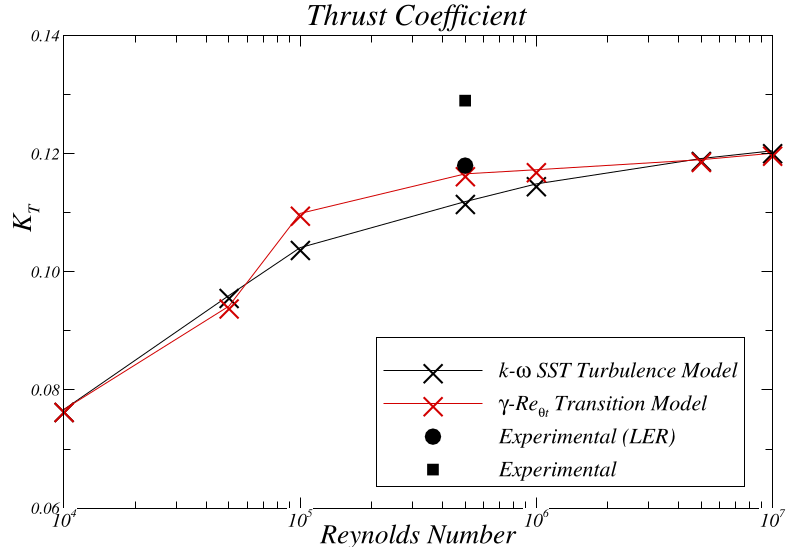
\includegraphics[width=\textwidth]{images/joroba_kt_joao.png}
        \caption{Coeficiente de empuje $K_T$.}
        \label{fig:joroba_kt_joao}
    \end{subfigure}
    \hfill
    \begin{subfigure}[b]{0.48\textwidth}
        \centering
        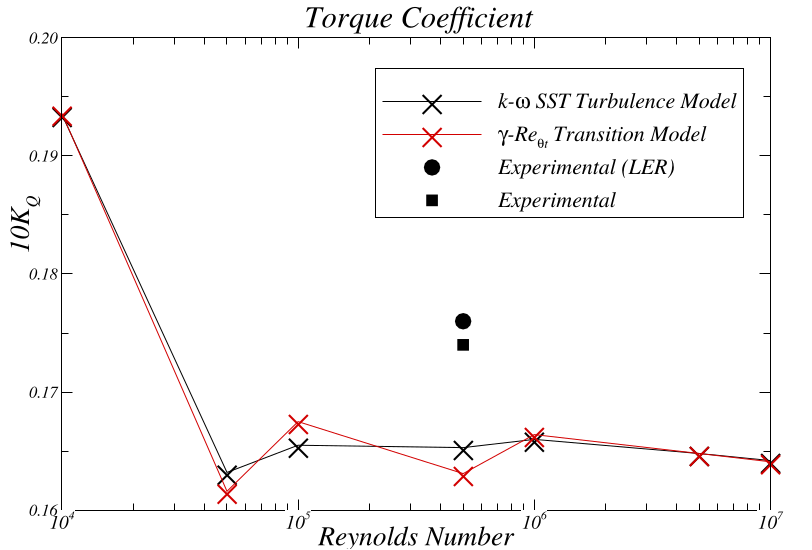
\includegraphics[width=\textwidth]{images/joroba_kq_joao.png}
        \caption{Coeficiente de par $K_Q$.}
        \label{fig:joroba_kq_joao}
    \end{subfigure}
    \caption{Coeficientes de empuje y de par frente al número de Reynolds
    seccional $Re_{c,0.7R}$. Adaptado de \citet{baltazar2018transition}.}
    \label{fig:joroba_joao}
\end{figure}
 
Las referencias fundamentales para la predicción numérica de este fenómeno son \citet{baltazar2018transition} y los trabajos de Gaggero. En \citet{baltazar2018transition} se compararon el modelo SST y el modelo de transición $\gamma$-$\widetilde{Re}_{\theta t}$ (descrito en la Sección~\ref{sec:modelos_transicion}) para dos hélices, obteniendo mejor acuerdo con los diagramas experimentales con el modelo de transición en el rango $Re_{c,0.7R} = 10^5$--$10^6$. Existen otros cierres de transición: en \citet{gaggero2018transition} se empleó en OpenFOAM el modelo $k$-$k_L$-$\omega$, que incorpora una ecuación de transporte adicional para la energía cinética de las fluctuaciones laminares $k_L$. Sus limitaciones fueron señaladas posteriormente en \citet{gaggero2021transition}: el cierre posterga la transición hasta números de Reynolds excesivamente altos --del orden de $2.3\times10^6$ para la hélice VP1304-- y resulta prácticamente insensible a la intensidad turbulenta impuesta en la entrada del dominio.

En \citet{gaggero2021transition} se retomaron esos mismos casos con el modelo $\gamma$-$\widetilde{Re}_{\theta t}$, resuelto tanto en OpenFOAM como en StarCCM+. De ese trabajo interesa aquí sobre todo un resultado: incluir la transición eleva \emph{tanto} $K_T$ \emph{como} $K_Q$ por encima de los valores totalmente turbulentos. Una capa límite parcialmente laminar reduce la fricción, y por sí sola debería producir un leve aumento del empuje junto con una caída más marcada del par; que ambos suban a la vez no se explica por esa vía y obliga a atribuir el efecto a la presión. El mecanismo propuesto es que, bajo capa límite laminar, las líneas de corriente sobre la pala adoptan una orientación predominantemente radial --por el predominio de la fuerza centrífuga-- que produce un efecto equivalente a un aumento de curvatura del perfil y eleva la succión en el dorso, en particular hacia el borde de salida; ese incremento de succión aporta simultáneamente empuje y par, y cancela el efecto favorable de la menor fricción. A diferencia del $k$-$k_L$-$\omega$, este cierre sí exhibe una sensibilidad apreciable a la intensidad turbulenta de entrada, cuestión que se retoma en la Sección~\ref{sec:modelos_transicion}.
 
La implicación directa para la extrapolación ITTC-78 es que, si el ensayo de modelo se realiza en el rango de la joroba, los valores de $K_T$ y $K_Q$ medidos no son representativos del comportamiento turbulento que el método asume y la corrección $\Delta C_D$ puede introducir errores sistemáticos de signo indefinido. Este argumento se desarrolla en el Capítulo~\ref{chap:helices} a través de la hélice P206, cuyos datos experimentales fueron provistos por Hanwha Ocean (empresa que además realizó la campaña experimental)
y que fue simulada numéricamente en el LabHiNO (Laboratorio de Hidrodinámica Naval y Oceánica, UBA). Sus $Re_{c,0.7R}$ de modelo se ubican precisamente en este rango conflictivo.
 
Vale la pena precisar por qué el estudio de este rango transicional tiene relevancia
práctica y no es meramente una curiosidad de laboratorio. En un ensayo de aguas
abiertas independiente, la recomendación práctica más directa frente a la joroba es,
simplemente, evitarlo: elegir un modelo de hélice de mayor diámetro o una velocidad
de giro más alta para que el ensayo caiga fuera del rango transicional, ya que no es
razonable extraer conclusiones hidrodinámicas generales --ni calibrar procedimientos
de extrapolación-- a partir de un régimen de capa límite que no es representativo del
comportamiento a escala buque. Sin embargo, esta salida no siempre está disponible.
En un ensayo autopropulsado, el modelo de hélice no se elige de forma independiente:
su escala queda determinada por la escala del modelo de casco, que a su vez está
acotada por las dimensiones del canal de ensayos (ancho, profundidad, velocidad
máxima del carro) y por la necesidad de mantener la semejanza de Froude con el buque
real. En esas condiciones, puede no existir ninguna combinación de escala de modelo y
condición de ensayo que evite el rango transicional del propulsor, y la joroba deja
de ser una condición evitable para convertirse en una limitación estructural del
ensayo. Es precisamente en ese escenario --cuando no queda otra escala disponible--
donde entender, predecir y corregir correctamente el comportamiento en esta zona deja
de ser opcional y se vuelve indispensable para no comprometer la validez de la
predicción a escala buque.
 
Esta cuestión se vincula, además, con una preocupación que la propia ITTC ha comenzado a documentar. La recomendación vigente fija un límite inferior de $Re_c(0.7R) = 2\times10^5$ para considerar un ensayo de aguas abiertas representativo \citep{ITTC_Performance_prediction}, pero \citet{heinke2019} muestran, para hélices de cuerda corta, que $K_T$ recién se estabiliza y deja de depender de $Re_c$ por encima de un valor sensiblemente mayor, del orden de $5\times10^5$, y que por debajo de ese umbral la extrapolación ITTC-78 produce curvas de escala buque poco confiables bajo flujo laminar o parcialmente laminar. Es decir, superar el límite recomendado de $2\times10^5$ no garantiza, por sí solo, que el ensayo se encuentre fuera del rango transicional. En consecuencia, sucesivos comités de la ITTC han alentado el uso de CFD para clarificar estos problemas de escalado y han revisado si el propio umbral de $2\times10^5$ es adecuado \citep{ittc2024rp}. Esta discusión se retoma en el Capítulo~\ref{chap:helices}, donde la campaña experimental analizada se ubica enteramente por encima de $2\times10^5$ y, sin embargo, exhibe una joroba medida con claridad.
 
\subsubsection{Modelado numérico de la transición: SST y SST-LM}
\label{sec:modelos_transicion}
 
El modelo $k$-$\omega$ SST de \citet{Menter1994}, cuyo desempeño en una amplia gama de aplicaciones industriales fue documentado por \citet{menter2003}, es el estándar de la industria para simulaciones viscosas de hélices a escala buque, donde el flujo es enteramente turbulento. Sin embargo, a Reynolds de escala modelo el SST fuerza la transición a un número de Reynolds excesivamente bajo, sobreestimando la extensión de la zona turbulenta y no reproduciendo la joroba \citep{baltazar2018transition}.
 
El modelo de transición $\gamma$-$\widetilde{Re}_{\theta t}$ (\textbf{SST-LM}), propuesto en \citet{langtry2009}, resuelve dos ecuaciones de transporte adicionales para la intermitencia $\gamma$ y el número de Reynolds de transición basado en el espesor de cantidad de movimiento $\widetilde{Re}_{\theta t}$, acopladas al SST. Es el modelo adoptado en las simulaciones de escala modelo del Capítulo~\ref{chap:helices}, por dos razones: ha demostrado mejor acuerdo con los datos experimentales de aguas abiertas en el rango transicional \citep{baltazar2018transition} y, al estar construido sobre la misma base SST empleada para las corridas totalmente turbulentas, permite atribuir las diferencias entre ambas soluciones al tratamiento de la transición y no a un cambio de cierre. Frente a alternativas como el $k$-$k_L$-$\omega$, esta continuidad de base es la que habilita la descomposición en presión y fricción del Capítulo~\ref{chap:helices}. Su principal limitación operativa es la alta sensibilidad a las condiciones de turbulencia de entrada (la intensidad turbulenta $Tu$ y la relación de viscosidad turbulenta $\mu_t/\mu$), que requieren calibración cuidadosa frente a los datos experimentales disponibles, tal como se describe en el Capítulo~\ref{chap:Metodologia}.
\chapter{Metodología Experimental y Numérica}
\label{chap:Metodologia}

\section{Introducción}

Habiendo establecido en el Capítulo 2 los fundamentos físicos de la resistencia al avance y las bases teóricas de la mecánica de fluidos, este capítulo detalla la implementación práctica de las herramientas utilizadas en esta tesis. La investigación adopta una estrategia híbrida que vincula ensayos físicos en canal de remolque (EFD) con simulaciones numéricas de alta fidelidad (CFD).

A continuación se describen las instalaciones experimentales del canal de pruebas del LabHiNO, las características geométricas de los modelos construidos y la instrumentación empleada. Posteriormente, se detalla la configuración del modelo numérico en ``OpenFOAM'', especificando el dominio computacional, las condiciones de contorno y los esquemas de discretización utilizados.

\section{Metodología Experimental (EFD)}

Los ensayos experimentales se llevaron a cabo en el canal de remolque de la Universidad de Buenos Aires (UBA), Argentina. Esta campaña tuvo como objetivo principal generar una base de datos de validación confiable para los modelos pesqueros P1, P2 y P3 y comparar los resultados con el buque de referencia KCS.

\subsection{Instalaciones: El Canal de Remolque}

Los ensayos se realizaron en el canal de remolque del LabHiNO. Esta instalación cuenta con un vaso de hormigón rectilíneo con las siguientes dimensiones principales:

\begin{itemize}
    \item \textbf{Longitud:} 72 m
    \item \textbf{Ancho:} 3.6 m
    \item \textbf{Profundidad:} 2.0 m
\end{itemize}

El canal está equipado con un carro dinamométrico capaz de alcanzar una velocidad máxima de 4.0 m/s, lo cual cubre holgadamente el rango de velocidades de Froude requeridas para los modelos analizados en este estudio.

\subsection{Modelos Físicos \label{sec:presentacion_modelos}}

Se fabricaron y ensayaron cuatro modelos a escala, de los cuales tres son pesqueros diseñados por astilleros argentinos y uno un portacontenedores de referencia. Todos fueron acabados con pintura de alto brillo para garantizar una superficie hidráulicamente lisa. A continuación se presentan los mismos.

\subsubsection{Modelo Pesquero 1}
El primer modelo estudiado, de ahora en más \textit{P1}, diseñado por el astillero ``TecnoPesca Argentina'', representa un buque pesquero de baja esbeltez ($L/B < 4$) característico de la flota nacional. El modelo fue construido a escala $\lambda = 20$.

En la Figura \ref{fig:model_tpa}, se presentan las vistas del modelo físico terminado. Se pueden apreciar las marcas de las diferentes secciones, lineas de agua y la disposición de la proa con bulbo. Para asegurar la transición a régimen turbulento de la capa límite y evitar la laminarización del flujo a bajas velocidades, se instalaron estimuladores de turbulencia (alambres cilíndricos de 3 mm de diámetro) a un 5\% de la eslora desde la perpendicular de proa, siguiendo las recomendaciones de la ITTC (Procedimiento 7.5-01-01-01).

\begin{figure}[htpb]
    \centering
    \begin{subfigure}[b]{0.48\textwidth}
        \centering
        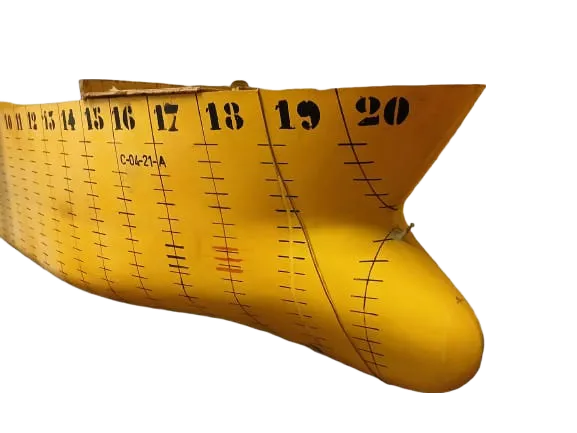
\includegraphics[width=\textwidth]{images/tpa-pers.png}
        \caption{Vista en perspectiva de proa. Se observan las marcas de calado y los estimuladores de turbulencia.}
        \label{fig:tpa_pers}
    \end{subfigure}
    \hfill
    \begin{subfigure}[b]{0.48\textwidth}
        \centering
        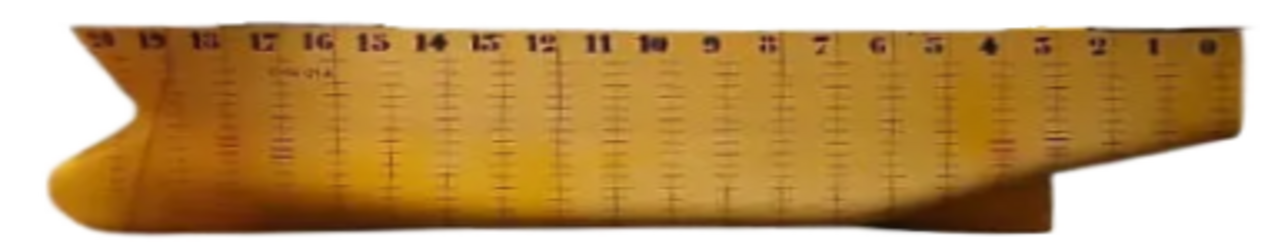
\includegraphics[width=\textwidth]{images/tpa-side.png}
        \caption{Vista de perfil. Geometría de baja esbeltez típica de pesqueros.}
        \label{fig:tpa_side}
    \end{subfigure}
    \caption{Modelo físico del pesquero TPA (Escala 1:20) preparado para ensayos en el LabHiNO.}
    \label{fig:model_tpa}
\end{figure}

El modelo se evaluó en tres condiciones de carga (ligero, medio y pesado) para barrer un rango operativo amplio y analizar la sensibilidad del factor de forma al calado. Las áreas transversales medias del modelo representaron el 1\%, 1.1\% y 1.2\% del área transversal del tanque para las condiciones de carga ligera, media y pesada, respectivamente.

La Tabla~\ref{tab:main_param_p1} resume las características geométricas y dinámicas del buque pesquero en escala real (T1) y del modelo en las tres condiciones de calado ensayadas (T1, T2 y T3).

\begin{table}[H]
\caption{Características principales del pesquero P1 en escala real y del modelo en tres condiciones de calado.}
\centering
\begin{tabularx}{\textwidth}{lllllll}
\toprule
\textbf{Característica}&\textbf{Símbolo}&\textbf{Unidad}&\textbf{Escala Real }&\textbf{Modelo} & \textbf{Modelo} & \textbf{Modelo}\\
 &  & & \textbf{T1} & \textbf{T1}& \textbf{T2} & \textbf{T3}\\
\midrule
Escala del modelo & $\lambda$ & {[}-{]} & - & 20 & 20 & 20\\
Eslora en flotación & L$_{WL}$ & {[}m{]} & 32.68 & 1.634 & 1.662 & 1.641\\
Eslora total sumergida & L$_{OS}$ & {[}m{]} & 34.795 & 1.670 & 1.740 & 1.740\\
Manga & B & {[}m{]} & 9.28 & 0.464 & 0.464 & 0.464\\
Calado & T & {[}m{]} & 3.30 & 0.165 & 0.180 & 0.195\\
Volumen de desplazamiento & V & {[}m$^3${]} & 599.40 & 0.075 & 0.085 & 0.095\\
Área de superficie mojada & S & {[}m$^2${]} & 392.67 & 0.982 & 1.058 & 1.124\\
Coeficiente de bloque & C$_B$ & {[}-{]} & 0.60 & 0.60 & 0.61 & 0.64\\
Desplazamiento (masa) & $\Delta$ & {[}t{]} & - & 75.0 & 85.0 & 95.0\\
\bottomrule
\end{tabularx}
\label{tab:main_param_p1}
\end{table}

\subsubsection{Modelo Pesquero 2}
El tercer pesquero analizado, de ahora en más P3, fue diseñado y construido por el Astillero Naval Federico Contessi y Cía. S.A. El modelo fue construido a escala $\lambda = 10$ y ensayado en una sola condición de calado. La Tabla~\ref{tab:main_param_p3} resume sus características principales.

\begin{table}[H]
\caption{Características principales del pesquero P3.}
\centering
\begin{tabularx}{\textwidth}{lllll}
\toprule
\textbf{Característica}&\textbf{Símbolo}&\textbf{Unidad} & \textbf{Escala Real} & \textbf{Modelo (T1)}\\
 &  &  & (Buque) &  \\
\midrule
Escala del modelo & $\lambda$ & {[}-{]} & - & 10 \\
Eslora en flotación& L$_{WL}$ & {[}m{]} & 25.100 & 2.510 \\
Eslora total sumergida & L$_{OS}$ & {[}m{]} & 26.580 & 2.658 \\
Manga & B & {[}m{]} & 7.800 & 0.780 \\
Calado & T & {[}m{]} & 3.460 & 0.346 \\
Volumen de desplazamiento & V & {[}m$^3${]} & 387.265 & 0.387 \\
Área de superficie mojada & S & {[}m$^2${]} & 292.000 & 2.920 \\
Coeficiente de bloque & C$_B$ & {[}-{]} & 0.577 & 0.571 \\
Desplazamiento (masa) & $\Delta$ & {[}t{]} & 397.295 & 387.0 \\
\bottomrule
\end{tabularx}
\label{tab:main_param_p2}
\end{table}

\subsubsection{Modelo Pesquero 3}
El segundo pesquero analizado, de ahora en más P2, fue diseñado y construido por el astillero JPA S.A. El modelo fue construido a escala $\lambda = 13$ y ensayado en una sola condición de calado. La Tabla~\ref{tab:main_param_p2} resume sus características principales.

\begin{table}[H]
\caption{Características principales del pesquero P2.}
\centering
\begin{tabularx}{\textwidth}{lllll}
\toprule
\textbf{Característica}&\textbf{Símbolo}&\textbf{Unidad} & \textbf{Escala Real} & \textbf{Modelo (T1)}\\
 &  &  & (Buque) &  \\
\midrule
Escala del modelo & $\lambda$ & {[}-{]} & - & 13 \\
Eslora en flotación & L$_{WL}$ & {[}m{]} & 22.050 & 1.696 \\
Eslora total sumergida & L$_{OS}$ & {[}m{]} & 22.282 & 1.714 \\
Manga & B & {[}m{]} & 7.800 & 0.600 \\
Calado & T & {[}m{]} & 3.050 & 0.235 \\
Volumen de desplazamiento & V & {[}m$^3${]} & 320.070 & 0.146 \\
Área de superficie mojada & S & {[}m$^2${]} & 240.964 & 1.426 \\
Coeficiente de bloque & C$_B$ & {[}-{]} & 0.643 & 0.608 \\
Desplazamiento (masa) & $\Delta$ & {[}t{]} & 328.360 & 146.0 \\
\bottomrule
\end{tabularx}
\label{tab:main_param_p3}
\end{table}


\subsubsection{Modelo de Referencia KCS}
Con el fin de complementar el análisis mediante la inclusión de un buque completamente diferente a los pesqueros, se construyó un modelo del portacontenedores ``KRISO Container Ship'' (KCS) a escala $\lambda = 79$. Este buque de alto valor referencial presenta características hidrodinámicas marcadamente distintas: una esbeltez muy superior (relación $L/B \approx 7.1$ vs. $L/B \approx 2.8$–$3.5$ para los pesqueros), una popa afinada con transición suave de cuerpo paralelo a codaste en contraste con la popa llena característica de los pesqueros, y la ausencia de dormido significativo frente al dormido pronunciado de los buques pesqueros. La Tabla~\ref{tab:main_param_kcs} resume sus características principales.

La Figura \ref{fig:model_kcs} muestra el modelo KCS, permitiendo comparar visualmente la geometría esbelta y refinada de este portacontenedores con la forma llena y robusta de los pesqueros argentinos. 

\begin{table}[H]
\caption{Características principales del portacontenedores KCS.}
\centering
\begin{tabularx}{\textwidth}{lllll}
\toprule
\textbf{Característica}&\textbf{Símbolo}&\textbf{Unidad} & \textbf{Escala Real} & \textbf{Modelo}\\
 &  &  & (Buque) & (T1) \\
\midrule
Escala del modelo & $\lambda$ & {[}-{]} & - & 79 \\
Eslora en flotación & L$_{WL}$ & {[}m{]} & 230.000 & 2.911 \\
Eslora total sumergida & L$_{OS}$ & {[}m{]} & 232.500 & 2.943 \\
Manga & B & {[}m{]} & 32.200 & 0.408 \\
Calado & T & {[}m{]} & 10.800 & 0.137 \\
Volumen de desplazamiento & V & {[}m$^3${]} & 52030.000 & 0.106 \\
Área de superficie mojada & S & {[}m$^2${]} & 9530.000 & 1.527 \\
Coeficiente de bloque & C$_B$ & {[}-{]} & 0.595 & 0.653 \\
Desplazamiento (masa) & $\Delta$ & {[}t{]} & 51925.940 & 105.318 \\
\bottomrule
\end{tabularx}
\label{tab:main_param_kcs}
\end{table}

\subsection{Instrumentación y Adquisición de Datos}

La medición de la resistencia total al avance ($R_T$) se realizó mediante una celda de carga de un solo componente marca \textbf{Kempf \& Remmers modelo R 47}. El transductor, diseñado para una carga a escala completa de $\pm 100$ N, posee una sensibilidad de aproximadamente $\pm 1$ mV/V de voltaje de alimentación.

El montaje del modelo al carro dinamométrico se realizó vinculándolo a la celda de carga de manera tal que se restringieron los movimientos de avance (velocidad constante impuesta por el carro), deriva, guiñada y rolido. El sistema permitió que el modelo quedara \textbf{libre a cabeceo (``trim'') y hundimiento (``sinkage'')}, conforme a los estándares para ensayos de resistencia al avance.

El sistema de adquisición de datos se configuró con los siguientes parámetros:
\begin{itemize}
    \item \textbf{Frecuencia de muestreo:} 200 Hz, permitiendo capturar la dinámica transitoria y las fluctuaciones.
    \item \textbf{Post-procesamiento:} Se aplicó un filtro paso bajo de 4 Hz a la señal para eliminar el ruido eléctrico y vibraciones mecánicas de alta frecuencia.
\end{itemize}

\subsection{Procedimiento de Ensayo y Análisis de Incertidumbre}

Se siguió el procedimiento estándar para ensayos de resistencia según la ITTC (7.5-02-02-01).

Dado que el modelo ocupa una fracción del volumen del canal, la presencia de las paredes y el fondo acelera el flujo alrededor del casco (efecto de bloqueo). Aunque las relaciones de área transversal fueron bajas ($1\% - 1.2\%$), se aplicó la \textbf{corrección de bloqueo de Schuster} a los resultados experimentales para garantizar la consistencia con la condición de aguas ilimitadas, de acuerdo con el procedimiento de la ITTC \cite{ITTC_resistance}.

\subsubsection*{Metodología de Análisis de Incertidumbre}
\label{sec:analisis_incertidumbre_general}

El análisis de incertidumbre para la medición de resistencia requiere la consideración exhaustiva de todas las fuentes significativas de error. El presente análisis sigue las directrices establecidas por la ITTC \cite{ITTC_uncertainty}, combinando componentes de incertidumbre mediante el método de la Raíz de la Suma de los Cuadrados (RSS, ``Root Sum Squares'').

\paragraph{Componentes de incertidumbre consideradas}

La resistencia total medida es función de múltiples variables independientes. Las incertidumbres se propagaron a través de cada una de estas dependencias:

\begin{itemize}
    \item \textbf{Geometría del casco:} La incertidumbre en el desplazamiento y la superficie mojada se cuantificó midiendo el lastre del modelo con una balanza de brazo portátil. Asumiendo que la incertidumbre geométrica no afecta significativamente el coeficiente de resistencia residual, la propagación ocurre a través de la superficie mojada y la eslora representativa. La incertidumbre estándar en la masa de desplazamiento constituye la fuente primaria para esta componente.

    \item \textbf{Velocidad de remolque:} Se consideró el límite de sesgo (``bias limit'') del carro dinamométrico. Este error se propaga a la medición de resistencia a través de la presión dinámica $q = \tfrac{1}{2}\rho V^2$ y en consecuencia al número de Reynolds. Para el rango operativo del LabHiNO, la precisión adoptada refleja la capacidad de control del sistema de remolque.

    \item \textbf{Temperatura del agua:} Dado que la viscosidad cinemática $\nu$ es fuertemente dependiente de la temperatura, variaciones de la misma afectan directamente al número de Reynolds $Re = \tfrac{V \cdot L}{\nu}$ y a la componente friccional de la resistencia. Se monitoreó la temperatura durante todos los ensayos. Las variaciones observadas se mantuvieron por debajo de $0.5\,^\circ$C, lo que implica variaciones en la viscosidad del orden del 2\% en el rango de interés.

    \item \textbf{Calibración del dinamómetro:} El transductor Kempf \& Remmers R47 se calibró antes y después de cada sesión de ensayo utilizando pesas patrón certificadas. Se ajustó una recta a los datos de calibración mediante regresión lineal, y la desviación estándar de esta regresión se adoptó como la incertidumbre estándar de calibración. Las pesas patrón empleadas fueron de precisión suficientemente alta como para considerarse su contribución despreciable.

    \item \textbf{Adquisición de datos (DAS):} La señal del dinamómetro se adquirió a frecuencia de muestreo de 200 Hz y fue filtrada mediante un filtro pasa bajos de 4 Hz antes de ingresar al sistema de adquisición. El promedio de cada ensayo se calculó sobre la historia temporal durante intervalos de al menos 10 segundos. La incertidumbre estándar del promedio temporal fue evaluada para cada repetición, resultando en valores entre $0.0007\%$ y $0.003\%$. Estos valores resultan despreciables en comparación con otras fuentes de error, confirmando la estabilidad del sistema de adquisición.

    \item \textbf{Repetibilidad:} Se realizaron múltiples repeticiones de cada ensayo a una misma velocidad. La media aritmética de estas repeticiones se adoptó como la mejor estimación de la resistencia. La incertidumbre estándar de la media de $N$ mediciones repetidas se estimó de acuerdo con el procedimiento de la ITTC, considerando tanto la dispersión entre repeticiones como el número de replicaciones.
\end{itemize}

\paragraph{Combinación de componentes mediante RSS}

Una vez estimadas todas las componentes individuales de incertidumbre, la incertidumbre combinada se calculó mediante:

\begin{equation}
u_c = \sqrt{u_1^2 + u_2^2 + \cdots + u_n^2}.
\end{equation}

La incertidumbre expandida, correspondiente a un nivel de confianza del 95\%, se obtuvo multiplicando la incertidumbre combinada por el factor de cobertura $k = 2$.

\paragraph{Comportamiento característico con el número de Froude}

Un hallazgo importante del análisis de incertidumbre es su dependencia funcional con la velocidad de remolque (o equivalentemente, con el número de Froude). A bajos números de Froude, la resistencia total es pequeña y la relación señal-ruido del dinamómetro se deteriora, amplificando la incertidumbre relativa. En este régimen, la calibración del dinamómetro y la dispersión entre repeticiones constituyen las fuentes dominantes. A medida que aumenta la velocidad, la resistencia total crece y la incertidumbre relativa disminuye, mejorando la relación señal-ruido.

Este comportamiento es consistente con lo esperado para ensayos de remolque y debe ser considerado en la comparación cuantitativa con resultados numéricos.

Los valores cuantitativos finales de la incertidumbre combinada y expandida para las distintas velocidades de ensayo específicas se presentan en detalle junto con los resultados experimentales en el Capítulo~\ref{cap:resistencia_factor_de_forma}.

\section{Procedimiento de extrapolación modelo--buque}
\label{sec:prediccion_potencia}

Una vez obtenida la resistencia del modelo mediante ensayos experimentales
o simulaciones numéricas, el paso siguiente consiste en extrapolar estos
resultados a escala buque. El procedimiento estándar recomendado por la
ITTC \citep{ITTC_Performance_prediction} se basa en la descomposición de
la resistencia total en sus componentes viscosa y de formación de olas,
escalando cada una de manera independiente.

El coeficiente de resistencia total del modelo se descompone como:
%
\begin{equation}
    C_{TM} = (1 + k_M)\,C_{FM0} + C_W ,
\end{equation}
%
donde $C_{FM0}$ es el coeficiente de fricción del modelo calculado mediante
la línea ITTC-57 (Sección~\ref{sec:ITTC57}) al número de Reynolds del modelo, $k_M$ es el factor de forma a escala modelo, determinado por el método de Prohaska como propone la ITTC \citep{ITTC_Performance_prediction}, por métodos empíricos, o según los métodos descritos en el Capítulo~\ref{cap:resistencia_factor_de_forma}, y $C_W$ es el coeficiente de resistencia por formación de olas, obtenido como residuo:
%
\begin{equation}\label{eq:CW_residuo}
    C_W = C_{TM} - (1+k_M)\,C_{FM0} .
\end{equation}
%
La hipótesis central del método es que $C_W$, así determinado, es
independiente del número de Reynolds y escala directamente con el número de
Froude. Bajo este supuesto, la resistencia total a escala buque se estima
como:
%
\begin{equation}\label{eq:CTS}
    C_{TS} = (1 + k_S)\,C_{FS0} + C_W + \Delta C_F + C_A + C_{AAS} ,
\end{equation}
%
\footnote{La corrección por rugosidad corresponde a la formulación de Townsin
y Dey, incorporada por la ITTC en 1990:
$\Delta C_F = 0.044\big[(k_s/L_{WL})^{1/3} - 10\,Re_S^{-1/3}\big] + 0.000125$,
donde $k_s$ es la altura de rugosidad equivalente (adoptada como
$k_s = 150\,\mu\text{m}$ en ausencia de mediciones directas) y $Re_S$ el
número de Reynolds del buque. El coeficiente de correlación, separado de la
rugosidad por el 19.\textsuperscript{o} ITTC, se calcula como
$C_A = (5.68 - 0.6\log_{10} Re_S)\times 10^{-3}$. Esta separación
reemplaza la formulación combinada original de Bowden y Davison
\citep{ITTC_Performance_prediction}.}

donde $C_{FS0}$ es el coeficiente de fricción del buque calculado mediante la línea ITTC-57 al número de Reynolds del buque, $k_S$ es el factor de forma a escala buque, $\Delta C_F$ es la corrección por rugosidad de la superficie, $C_A$ es el coeficiente de correlación modelo--buque y $C_{AAS}$ es el coeficiente de resistencia aerodinámica de la obra muerta, todos evaluados según las formulaciones recomendadas por la ITTC
\citep{ITTC_Performance_prediction}.

Conviene subrayar la estructura de las Ecuaciones~\eqref{eq:CW_residuo}
y~\eqref{eq:CTS}: la resistencia por olas $C_W$ se calcula con el factor de
forma de modelo $k_M$ y se traslada sin modificación a la escala buque,
mientras que la componente viscosa se escala con el factor de forma de buque $k_S$. El método estándar de la ITTC asume $k_S = k_M$, es decir, un factor de forma independiente de la escala, con lo que ambas ecuaciones se reducen al procedimiento clásico de un único factor de forma. Cuando, en cambio, se admite $k_S \neq k_M$, la formulación coincide con el método de dos factores de forma ($2k$) de \citet{korkmaz_wetted_transom}, en el que la componente viscosa se corrige por efectos de escala sin alterar la residual. Como se analiza en profundidad en el Capítulo~\ref{cap:resistencia_factor_de_forma}, la hipótesis $k_S = k_M$ no se cumple para los pesqueros estudiados en esta tesis, lo que hace necesario el uso de la formulación de dos factores de forma.

La resistencia total del buque y la potencia efectiva se obtienen como:
%
\begin{equation}
    R_{TS} = \tfrac{1}{2}\,\rho\,V_S^2\,S_S\,C_{TS},
\end{equation}
%
\begin{equation}
    P_{ES} = R_{TS}\,V_S,
\end{equation}
%
donde $\rho$ es la densidad del agua, $V_S$ la velocidad del buque y $S_S$
la superficie mojada a escala buque.

\section{Metodología Numérica (CFD)}

Las simulaciones numéricas se realizaron utilizando el código de código abierto \textbf{OpenFOAM} (versión 11), basado en el Método de Volúmenes Finitos (FVM).

\subsection{Dominio Computacional y Mallado}

Se definió un dominio computacional rectangular prismático dimensionado para evitar la reflexión de olas.
\begin{itemize}
    \item \textbf{Entrada (Inlet):} Ubicada a $1.5 L_{pp}$ a proa del modelo.
    \item \textbf{Salida (Outlet):} Ubicada a $2.5 L_{pp}$ a popa.
    \item \textbf{Límites laterales y fondo:} Ubicados a distancia suficiente para simular aguas profundas.
\end{itemize}

El mallado se generó con \texttt{snappyHexMesh}, utilizando una estructura predominantemente hexaédrica no estructurada con refinamientos locales en la superficie libre y la estela, e inserción de capas de prismas en la superficie del casco para resolver la capa límite ($y^+$ controlado).

\subsection{Configuración de los Casos de Estudio}

Se emplearon dos configuraciones de simulación distintas. A continuación se detallan las condiciones de contorno específicas seleccionadas para garantizar la estabilidad y conservación de masa en el dominio.

\subsubsection{Simulación con Superficie Libre}
Esta configuración replica el ensayo de canal para obtener la resistencia total ($R_T$) y el campo de olas.

\begin{itemize}
    \item \textbf{Solucionador:} \texttt{interFoam} (VoF con compresión de interfaz MULES).
    \item \textbf{Algoritmo:} PIMPLE (híbrido PISO-SIMPLE).
\end{itemize}

La Figura \ref{fig:dominio_metodologia} esquematiza el dominio computacional utilizado, mostrando la disposición de las condiciones de contorno.

\begin{figure}[htpb]
    \centering
    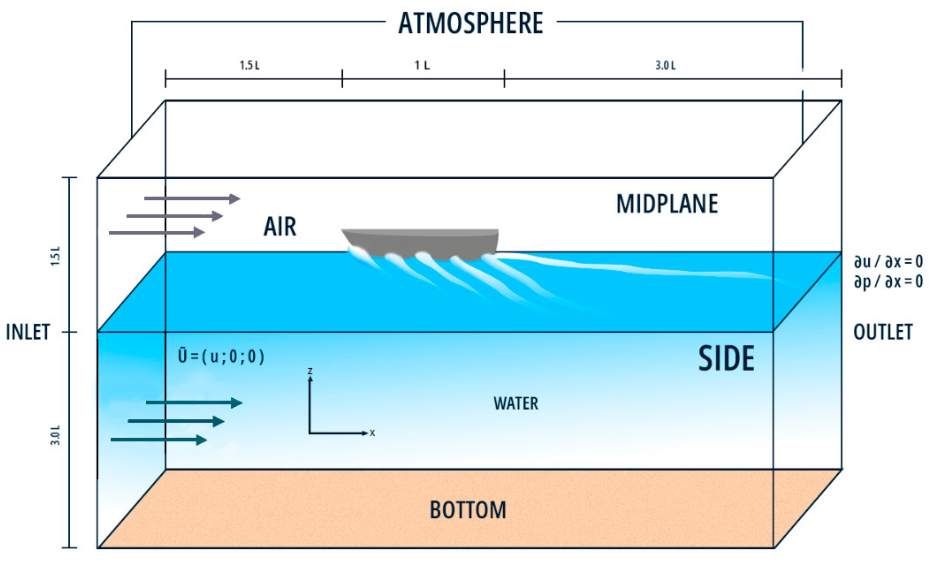
\includegraphics[width=0.6\textwidth]{images/domain.png}
    \caption{Dominio computacional y condiciones de contorno para las simulaciones de resistencia con superficie libre.}
    \label{fig:dominio_metodologia}
\end{figure}

Las condiciones de borde específicas se resumen en la Tabla \ref{tab:bc_setup}.

\begin{table}[H]
\centering
\caption{Condiciones de borde específicas para las simulaciones con superficie libre (VoF).}
\label{tab:bc_setup}
\small
\begin{tabular}{lcccc}
\toprule
\textbf{Variable} & \textbf{Entrada} & \textbf{Salida} & \textbf{Atmósfera} & \textbf{Casco} \\
\midrule
$U$ & FV & OPMV & PIOV & MWV \\
$p_{rgh}$ & FFP & ZG & TP & FFP \\
$\alpha_{water}$ & FV & VHFR & IO & ZG \\
$k$ & FV & IO & IO & kLRWF \\
$\omega$ & FV & IO & IO & oWF \\
$\nu_t$ & calc. & calc. & calc. & nutkWF \\
\bottomrule
\end{tabular}
\end{table}

\noindent\textbf{Definición de condiciones de borde:}
\begin{itemize}
    \item \textbf{FV} (\texttt{fixedValue}): Valor fijo.
    \item \textbf{ZG} (\texttt{zeroGradient}): Gradiente nulo.
    \item \textbf{IO} (\texttt{inletOutlet}): Permite flujo reverso.
    \item \textbf{FFP} (\texttt{fixedFluxPressure}): Ajusta gradiente de presión por flujo másico.
    \item \textbf{OPMV} (\texttt{outletPhaseMeanVelocity}): Velocidad media de fase en salida.
    \item \textbf{PIOV} (\texttt{pressureInletOutletVelocity}): Velocidad dependiente de presión.
    \item \textbf{TP} (\texttt{totalPressure}): Presión total fija.
    \item \textbf{MWV} (\texttt{movingWallVelocity}): Velocidad de pared (cero relativo).
    \item \textbf{VHFR} (\texttt{variableHeightFlowRate}): Altura variable de superficie libre.
    \item \textbf{kLRWF} / \textbf{oWF} / \textbf{nutkWF}: Funciones de pared para turbulencia.
\end{itemize}

\subsubsection{Simulación de Doble Cuerpo}\label{sec:doble_cuerpo}

Esta configuración se utiliza exclusivamente para aislar la resistencia viscosa ($R_V$) y determinar el factor de forma $(1+k)$. El término ``Doble Cuerpo'' hace referencia al concepto aerodinámico de reflejar el casco sumergido respecto al plano de flotación, generando un cuerpo equivalente completamente sumergido en un fluido infinito.

\paragraph{Fundamento Físico y Dominio}
En esta aproximación, la superficie libre se sustituye por una condición de \textbf{tapa rígida sin fricción} (``frictionless rigid lid''). Geométricamente, el dominio se trunca en la línea de flotación estática ($z=0$), tal como se ilustra en la Figura \ref{fig:double_body_domain}.

\begin{figure}[htpb]
    \centering
    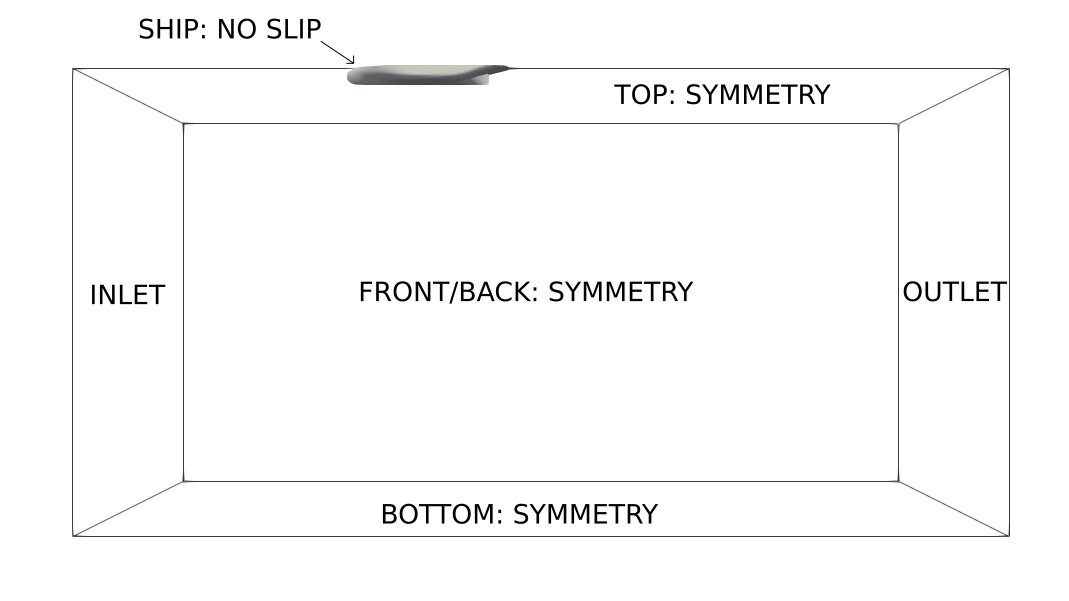
\includegraphics[width=0.6\textwidth]{images/esquema_malla}
    \caption{Dominio reducido para simulación sin superficie libre (Doble Cuerpo), mostrando la condición de simetría en el plano de flotación.}
    \label{fig:double_body_domain}
\end{figure}

\begin{itemize}
    \item \textbf{Plano de Simetría:} La frontera superior del dominio se define como un \texttt{symmetryPlane}. Matemáticamente, esto impone dos restricciones fundamentales:
    \begin{enumerate}
        \item Flujo impenetrable: La componente normal de la velocidad es nula ($\mathbf{v} \cdot \mathbf{n} = 0$).
        \item Cero esfuerzo cortante: El gradiente normal de la velocidad tangencial es nulo ($\partial \mathbf{v}_t / \partial n = 0$).
    \end{enumerate}
    Esta configuración elimina la generación de olas ($R_W = 0$) y la energía potencial gravitatoria, permitiendo que la presión calculada corresponda únicamente a la presión hidrodinámica viscosa.
\end{itemize}

\paragraph{Ventajas del Mallado}
Al eliminar la necesidad de capturar la interfase aire-agua, se prescinde del refinamiento de malla vertical en la zona de superficie libre. Esto permite concentrar la densidad de celdas en la capa límite y, crucialmente, en la \textbf{estela viscosa} y la zona de recirculación del espejo de popa (``transom''), optimizando el costo computacional global frente a las simulaciones VoF.

\paragraph{Configuración Numérica (PIMPLE)}
A diferencia de los enfoques estacionarios clásicos, en este trabajo se utilizó un solucionador transitorio (\textbf{\texttt{pimpleFoam}}) para resolver las ecuaciones RANS monofásicas.
\begin{itemize}
    \item \textbf{Justificación:} Se optó por la resolución transitoria para garantizar la estabilidad numérica frente a desprendimientos de flujo complejos y oscilantes en la zona del espejo de popa, los cuales suelen dificultar la convergencia de solucionadores estacionarios (tipo SIMPLE).
    \item \textbf{Algoritmo:} Se utilizó el algoritmo PIMPLE, que permite utilizar pasos de tiempo grandes ($Co_{max} > 1$) manteniendo la estabilidad mediante correcciones externas en cada paso de tiempo.
    \item \textbf{Convergencia:} La simulación se ejecutó hasta alcanzar un estado cuasi-estacionario donde las fuerzas hidrodinámicas oscilan en torno a un valor medio constante.
\end{itemize}

\paragraph{Cálculo del Factor de Forma}
La resistencia viscosa total $R_V$, compuesta por la fricción tangencial $R_F$
y la presión viscosa $R_{PV}$, se obtuvo promediando la señal de resistencia
en el intervalo de tiempo convergido. El factor de forma se determina como:
%
\begin{equation}
    (1+k) = \frac{C_V}{C_{F0}},
\end{equation}
%
donde $C_V = C_F + C_{PV}$ es el coeficiente de resistencia viscosa
obtenido de la simulación de doble cuerpo y $C_{F0}$ es el coeficiente
de la línea ITTC-57, definido en la Sección~\ref{sec:ITTC57}. Se adopta la
línea ITTC-57 como referencia de $C_{F0}$ para preservar la coherencia con
los factores de correlación históricos, siguiendo la recomendación de la
ITTC \citep{ITTC_Combined_2021}. El valor del factor de forma resultante
depende, no obstante, de la línea de fricción elegida, y estudios recientes
que emplean líneas de fricción numéricas \citep{quintuna2023} obtienen
factores de forma sistemáticamente mayores y menos dependientes de la escala,
por lo que los valores aquí reportados deben interpretarse siempre en
relación con la línea de referencia empleada.

\subsection{Modelado de la Turbulencia: Modelo $k$--$\omega$ SST}
\label{sec:metodo_SST}

Para el cierre del sistema de ecuaciones RANS, se seleccionó el modelo \textbf{$k$--$\omega$ SST (Shear Stress Transport)}, desarrollado en \citet{Menter1994}. Este modelo se ha convertido en el estándar de la industria naval debido a su capacidad para predecir con mayor precisión el inicio y la magnitud de la separación del flujo bajo gradientes de presión adversos, una característica crítica en la hidrodinámica de popas de buques pesqueros.

El modelo SST es una formulación híbrida de dos ecuaciones que resuelve el transporte de la energía cinética turbulenta ($k$) y la tasa específica de disipación ($\omega$). Su principal ventaja radica en la combinación zonal: utiliza la robusta formulación original $k$--$\omega$ de Wilcox en la región cercana a la pared (capa límite) y conmuta al modelo estándar $k$--$\varepsilon$ en la región de flujo libre. Esta estrategia evita la conocida sensibilidad del modelo $k$--$\omega$ a las condiciones de turbulencia en el borde de entrada (``freestream sensitivity'').

Las ecuaciones de transporte para $k$ y $\omega$ en el modelo SST son:

\begin{equation}
    \frac{\partial (\rho k)}{\partial t} + \frac{\partial (\rho U_i k)}{\partial x_i} = \tilde{P}_k - \beta^* \rho k \omega + \frac{\partial}{\partial x_i} \left[ (\mu + \sigma_k \mu_t) \frac{\partial k}{\partial x_i} \right],
\end{equation}

\begin{equation}
    \frac{\partial (\rho \omega)}{\partial t} + \frac{\partial (\rho U_i \omega)}{\partial x_i} = \alpha \rho S^2 - \beta \rho \omega^2 + \frac{\partial}{\partial x_i} \left[ (\mu + \sigma_\omega \mu_t) \frac{\partial \omega}{\partial x_i} \right] + 2(1-F_1) \rho \sigma_{\omega 2} \frac{1}{\omega} \frac{\partial k}{\partial x_i} \frac{\partial \omega}{\partial x_i},
\end{equation}

donde $\rho$ es la densidad del fluido, $U_i$ la componente $i$ de la
velocidad, $\mu$ la viscosidad dinámica molecular, $\mu_t$ la viscosidad
turbulenta dinámica, $\tilde{P}_k$ el término de producción limitado de
turbulencia, $F_1$ la función de mezcla del modelo SST, y $\sigma_k$,
$\sigma_\omega$, $\beta$, $\beta^*$ y $\alpha$ son coeficientes del modelo
interpolados mediante $F_1$ entre los valores de los modelos
$k$--$\omega$ y $k$--$\varepsilon$.

El último término de la ecuación de $\omega$ representa la \textbf{difusión cruzada} (``cross-diffusion''), que se activa únicamente en la zona de flujo libre ($F_1 \to 0$), permitiendo transformar matemáticamente el modelo $k$--$\varepsilon$ en una formulación basada en $\omega$.

\paragraph{Definición de la Viscosidad Turbulenta}
La diferencia fundamental del modelo SST respecto a los modelos estándar radica en la definición de la viscosidad turbulenta ($\nu_t$). En las capas límite sujetas a gradientes de presión adversos, la hipótesis estándar de Boussinesq sobreestima el esfuerzo cortante de Reynolds, lo que conduce a una predicción tardía de la separación del flujo.

Para corregir esto, Menter introdujo un limitador basado en la hipótesis de Bradshaw, que establece que el esfuerzo cortante es proporcional a la energía cinética turbulenta en la mayor parte de la capa límite. La viscosidad turbulenta se calcula como:

\begin{equation}
    \nu_t = \frac{a_1 k}{\max(a_1 \omega, S F_2)},
\end{equation}

donde:
\begin{itemize}
    \item $S = \sqrt{2 S_{ij} S_{ij}}$ es la magnitud del invariante de la tasa de deformación, con $S_{ij} = \tfrac{1}{2}(\partial U_i/\partial x_j + \partial U_j/\partial x_i)$ el tensor de tasa de deformación.
    \item $a_1 = 0.31$ es una constante empírica (coeficiente de estructura de Bradshaw).
    \item $F_2$ es una segunda función de mezcla que restringe el limitador a la capa límite.
\end{itemize}

Esta formulación asegura que $\nu_t$ no crezca excesivamente en zonas de alta deformación y baja vorticidad, permitiendo capturar correctamente la estructura de la estela y los vórtices en la popa del buque.

\paragraph{Tratamiento de Pared}
{\sloppy
En las superficies del casco, se emplearon condiciones de borde tipo función de pared adaptativa disponibles en ``OpenFOAM'' (\texttt{kLowReWallFunction}, \texttt{omegaWallFunction}). Estas condiciones permiten una transición continua entre la integración directa de las ecuaciones hasta la pared (cuando la malla es fina, $y^+ \approx 1$) y el uso de leyes de pared logarítmicas (cuando $y^+ > 30$), asegurando la robustez de la solución independientemente de las variaciones locales de la calidad de la malla.
\par}

\section{Metodología Numérica para Hélices en Aguas Abiertas}
\label{sec:metodologia_helices}

A diferencia de las simulaciones de resistencia del casco descriptas en la sección
anterior, las simulaciones de hélices en aguas abiertas se resuelven en un marco de
referencia solidario a la rotación del propulsor, sin superficie libre. Con el
objetivo de evaluar la robustez de las predicciones frente a la elección del código
de cálculo, este tipo de simulaciones se realizó en paralelo con dos solvers RANS de
naturaleza distinta --StarCCM+ (comercial, solver acoplado) y OpenFOAM (código
abierto, solver segregado)-- cuya configuración específica se detalla a
continuación. Los casos de estudio particulares (geometría de la hélice, rango de
$Re_n$ o $Re_c$ explorado, niveles de intensidad turbulenta ensayados) se presentan en
el Capítulo~\ref{chap:helices} junto con los resultados.

En ambos códigos se emplearon los mismos dos modelos de turbulencia introducidos en la
Sección~\ref{sec:metodo_SST}: el modelo $k$--$\omega$ SST completamente turbulento
como referencia, y el modelo de transición SST-LM
($\gamma$--$\widetilde{Re}_{\theta t}$) de \citet{langtry2009}, que resuelve dos
ecuaciones de transporte adicionales para la intermitencia $\gamma$ y el número de
Reynolds de inicio de transición $\widetilde{Re}_{\theta t}$, acopladas al modelo SST
base.

\subsection{Configuración en StarCCM+}
\label{sec:metodologia_helices_starccm}

Las simulaciones se resuelven en marco de referencia en rotación, empleando las
ecuaciones RANS estacionarias. El dominio y el mallado específicos de cada caso
(dimensiones, densidad de celdas, tratamiento de capa límite) se detallan junto con
cada campaña de simulaciones en el Capítulo~\ref{chap:helices}.

\subsection{Configuración en OpenFOAM}
\label{sec:metodologia_helices_openfoam}

Las simulaciones se realizaron con \textbf{OpenFOAM~8}, empleando el solver
estacionario \texttt{simpleFoam} (algoritmo SIMPLE) sobre un dominio reducido de
$90^\circ$ que modela una única pala, con la periodicidad impuesta mediante una
interfaz de malla móvil (AMI) y el efecto de la rotación incorporado a través de la
formulación de Marco de Referencia Múltiple (MRF). El modelo SST-LM se implementó
utilizando la formulación \texttt{kOmegaSSTLM} disponible de forma nativa en
OpenFOAM~8.

La malla se generó íntegramente dentro del entorno OpenFOAM, combinando
\texttt{cfMesh} para la discretización de la geometría base y \texttt{snappyHexMesh}
para la inserción de las capas de prismas en la superficie del álabe, con un $y^+$
objetivo menor a 2 en promedio --requisito para el correcto funcionamiento del modelo
de transición--, aunque en algunas zonas puntuales se alcanzaron valores de hasta 3.
La cantidad de capas de prismas específica de cada caso se detalla en el
Capítulo~\ref{chap:helices}. La discretización espacial emplea esquemas de segundo
orden acotados (\texttt{bounded Gauss linearUpwindV} para el término convectivo de
momento, \texttt{Gauss upwind} para $k$, $\omega$, $\gamma$ y
$\widetilde{Re}_{\theta t}$), con gradientes calculados mediante
\texttt{cellMDLimited Gauss linear} y distancia a la pared evaluada con el método
\texttt{meshWave}. En la entrada se impusieron condiciones de tipo
\texttt{fixedValue} para $k$, $\omega$ y $\widetilde{Re}_{\theta t}$.

\subsection{Calibración de la intensidad turbulenta}
\label{sec:metodologia_helices_tu}

Las simulaciones con SST-LM requieren especificar el nivel de intensidad turbulenta
($Tu$) en el plano del disco, parámetro del cual depende fuertemente el punto de
inicio de la transición laminar-turbulenta. Siguiendo la metodología de
\citet{Gaggero2020}, en ambos códigos las variables de turbulencia se mantienen
congeladas desde la entrada del dominio hasta una distancia de $0.5D$ aguas arriba de
la hélice, permitiendo su decaimiento únicamente en el tramo restante de $0.5D$ hasta
el plano del disco. De este modo, $Tu$ en el disco --y no en la entrada-- es el
parámetro físicamente relevante y comparable entre ambos solvers, independientemente
de las diferencias de formulación de cada código. Tal como se documenta en
\citet{Baltazar2021}, la relación de viscosidad turbulenta $\mu_t/\mu$ en la entrada
se ajusta para controlar esa tasa de decaimiento; una vez fijado el $Tu$ objetivo en
el disco, variaciones adicionales de $\mu_t/\mu$ producen efectos secundarios sobre
las predicciones de fuerza que deben tenerse en cuenta al interpretar la sensibilidad
de los resultados a este parámetro.

\section{Estrategia de Verificación y Validación (V\&V)}

Para garantizar la fiabilidad de los resultados numéricos y cuantificar la incertidumbre de la simulación, se siguió el procedimiento estándar recomendado por la ITTC \cite{ITTC_uncertainty_CFD} y la ASME \cite{asme}, basado en las directrices de \citet{freitas}.

\subsection{Estudio de Convergencia de Malla (GCI)}
\label{sec:convergencia_de_malla}

Se realizó un estudio de independencia de malla utilizando el método del Índice de Convergencia de Malla (GCI, ``Grid Convergence Index''). Este método, basado en la extrapolación de Richardson, permite cuantificar el error de discretización y evaluar la proximidad de la solución numérica al valor asintótico.

El estudio se llevó a cabo utilizando tres mallas sistemáticamente refinadas: gruesa (``coarse'', índice 3), media (``medium'', índice 2) y fina (``fine'', índice 1). La relación de refinamiento $r$ entre mallas sucesivas se mantuvo constante en $r = \sqrt{2}$, definida como:

\begin{equation}
r = \frac{h_{3}}{h_{2}} = \frac{h_{2}}{h_{1}} \approx \sqrt{2},
\end{equation}

donde $h$ representa el tamaño característico de la celda.

\subsubsection{Procedimiento de Cálculo}

En primer lugar, se define la diferencia de la solución numérica entre dos mallas sucesivas. Siendo $\Phi$ la variable de interés (en este caso, el factor de forma $1+k$ o la resistencia total), se calcula:

\begin{equation}
    \epsilon_{21} = \Phi_{2} - \Phi_{1}, \qquad \epsilon_{32} = \Phi_{3} - \Phi_{2},
\end{equation}

donde los subíndices indican la malla correspondiente (1: fina, 2: media,
3: gruesa). A partir de estas diferencias, se calcula la razón de
convergencia $R$:

\begin{equation}
    R = \frac{\epsilon_{21}}{\epsilon_{32}}.
\end{equation}

Siguiendo los criterios establecidos por la ITTC (2008), el comportamiento de la convergencia se clasifica de la siguiente manera:
\begin{itemize}
    \item \textbf{Convergencia Monotónica ($0 < R < 1$):} La solución se acerca al valor asintótico de manera uniforme.
    \item \textbf{Convergencia Oscilatoria ($R < 0$):} La solución oscila alrededor del valor asintótico. En este caso, la incertidumbre se estima basándose en la amplitud de la oscilación.
    \item \textbf{Divergencia ($R > 1$):} La solución se aleja al refinar la malla (caso no válido).
\end{itemize}

Para los casos de convergencia (monotónica u oscilatoria acotada), se calcula el orden aparente de precisión $p$:

\begin{equation}
    p = \frac{\ln \left( \frac{\epsilon_{32}}{\epsilon_{21}} \right)}{\ln(r)}.
\end{equation}

Finalmente se determina el Índice de Convergencia de Malla para la malla fina ($GCI_{fine}$):

\begin{equation}
    GCI_{fine} = F_s \frac{ \left| \frac{\Phi_{1} - \Phi_{2}}{\Phi_{1}} \right| }{r^p - 1} \times 100 \%,
\end{equation}

donde $F_s = 1.25$ es el factor de seguridad recomendado por la ITTC
para estudios con tres mallas \citep{ITTC_uncertainty_CFD}.

Basado en este procedimiento, se seleccionó la \textbf{malla fina} para todas
las simulaciones de producción presentadas en esta tesis. Los valores de
verificación resultantes (razón de convergencia $R$, orden aparente $p$,
resolución de pared $y^+$ e índice $GCI$ para cada velocidad y escala) se
presentan junto con los resultados correspondientes en cada capítulo, de modo
que todo caso de estudio incluye su propia verificación numérica: la
verificación del factor de forma y la resistencia se detalla en el
Capítulo~\ref{cap:resistencia_factor_de_forma}, y la de los ensayos de
propulsión en el Capítulo~\ref{chap:helices}.
\chapter{Resistencia al avance — Factor de forma} \label{cap:resistencia_factor_de_forma}
\mtcsettitle{minitoc}{Contenidos} 
\minitoc

\section{Determinación experimental y numérica del factor de forma}
\subsection{Ensayos experimentales de resistencia al avance}

\subsubsection{Introducción general}

La presente sección aborda la construcción de la curva de resistencia y el cálculo del factor de forma $(1+k)$ a partir de ensayos experimentales realizados en el canal del Laboratorio de Hidrodinámica Naval y Oceánica (LabHiNO). El objetivo específico de esta etapa es generar un conjunto de datos experimentales reproducibles que sirvan como base para la posterior comparación con resultados numéricos y para el análisis de efectos de escala que se desarrollará más adelante.

Si bien los fundamentos teóricos, los criterios de similitud y los antecedentes metodológicos fueron discutidos previamente en los Capítulos \ref{chap:antecedentes} y \ref{chap:Metodologia}, esta sección constituye el primer punto donde dicha metodología se aplica de manera operativa. En particular, se detalla la campaña experimental realizada sobre el modelo \textit{P1}, mostrando los criterios de adquisición, la repetibilidad, el control de condiciones del canal y la estimación de incertidumbres asociadas. Estos elementos permiten evaluar la calidad de los datos y establecen un marco sólido para la comparación cuantitativa con los resultados CFD presentados en secciones posteriores.

Asimismo, aunque esta sección se centra inicialmente en el modelo objetivo (\textit{P1}), el análisis experimental incluye también una campaña independiente con el modelo del portacontenedores KCS, presentada más adelante. La incorporación de este buque de referencia obedece al interés de complementar el análisis mediante la inclusión de una geometría radicalmente distinta a los pesqueros: una esbeltez mucho mayor ($L/B \approx 7.1$ vs. 2.8–3.5), una popa afinada con transición suave al codaste en contraste con la popa robusta de los pesqueros, y la ausencia de dormido significativo frente al dormido pronunciado de los buques pesqueros. Esta comparación permite examinar cómo la hidrodinámica del factor de forma varía cuando se introducen cambios fundamentales en las proporciones globales y la configuración local del casco.

\vspace{1em}

\subsubsection{Modelo \textit{P1}}

\paragraph{Ensayo de resistencia al avance}

El modelo \textit{P1}, presentado en la Sección \ref{sec:presentacion_modelos}, representa un buque pesquero de baja esbeltez, construido en escala 1:20 y ensayado en tres condiciones de calado: ligero, medio y pesado.
Cada ensayo se realizó siguiendo los procedimientos recomendados por la ITTC \citep{ITTC_resistance}, manteniendo libre el trimado y el hundimiento.
La resistencia total se midió mediante una celda de carga Kempf \& Remmers R47, con adquisición a 200~Hz y filtrado de 4~Hz.

\paragraph{Análisis de incertidumbre}

El análisis de incertidumbre para los ensayos del modelo \textit{P1} sigue la metodología general detallada en la Sección~\ref{sec:analisis_incertidumbre_general}. Se realizaron cuatro repeticiones independientes de cada ensayo a cada velocidad, permitiendo evaluar tanto la dispersión entre ensayos como las incertidumbres instrumentales asociadas.

En el modelo \textit{P1}, las fuentes dominantes de incertidumbre resultan ser la calibración del dinamómetro R47 y la dispersión entre repeticiones. La contribución relativa de estas componentes disminuye significativamente con el número de Froude: a $Fr = 0.14$, donde la resistencia total es mínima, la relación señal-ruido se deteriora y la incertidumbre relativa alcanza su máximo; a medida que aumenta la velocidad hacia $Fr = 0.37$, la resistencia crece cuadráticamente y la incertidumbre relativa desciende pronunciadamente. Este comportamiento es característico de ensayos de remolque y está cualitativamente acorde con el desempeño esperado.

La combinación de todas las componentes mediante el método RSS (Sección~\ref{sec:analisis_incertidumbre_general}) arrojó incertidumbres combinadas de $5.35\%$, $2.04\%$ y $0.83\%$ para $Fr = 0.14$, $0.26$ y $0.37$ respectivamente, niveles adecuados y consistentes con las recomendaciones de la ITTC. La Tabla~\ref{tab:uncert_tpa} presenta el desglose detallado de todas las componentes consideradas.

\begin{table}[H]
\caption{Resumen de incertidumbre combinada en las mediciones de resistencia
del modelo \textit{P1}.}
\begin{tabularx}{\textwidth}{lccc}
\toprule
\textbf{Componente} & \textbf{Fr = 0.14} & \textbf{Fr = 0.26} & \textbf{Fr = 0.37} \\
\midrule
Geometría del casco              & 0.05\% & 0.05\% & 0.05\% \\
Velocidad de remolque            & 0.07\% & 0.07\% & 0.07\% \\
Temperatura del agua             & 0.03\% & 0.03\% & 0.03\% \\
Calibración del dinamómetro      & 4.73\% & 1.04\% & 0.35\% \\
Repetibilidad (desviación) $^a$  & 5.00\% & 3.50\% & 1.50\% \\
\midrule
Incertidumbre combinada (ensayo único)
                                 & 6.88\% & 3.65\% & 1.54\% \\
Repetibilidad (desviación de la media)
                                 & 2.50\% & 1.75\% & 0.75\% \\
\textbf{Incertidumbre combinada (media de 4 rep.)}
    & \textbf{5.35\%} & \textbf{2.04\%} & \textbf{0.83\%} \\
Incertidumbre expandida (media de 4 rep.)
                                 & 10.70\% & 4.08\% & 1.66\% \\
\bottomrule
\end{tabularx}
\footnotesize{[$^a$] Repetibilidad (desviación) = Repetibilidad (desviación de
la media) $\times N^{1/2}$.}
\label{tab:uncert_tpa}
\end{table}

Las Figuras~\ref{fig:resis_tpa_165} a \ref{fig:resis_tpa_195} muestran las curvas de resistencia total obtenidas para cada uno de los calados ensayados. En todos los casos se observa el comportamiento esperado para un modelo de buque de desplazamiento: la resistencia crece de manera aproximadamente cuadrática con la velocidad en el rango de bajos números de Froude, donde domina la componente viscosa, y aumenta con mayor pendiente a partir de aproximadamente $Fr \approx 0.30$, donde la componente de generación de olas, proporcional a una potencia entre 2 y 4 de $Fr$, comienza a adquirir mayor relevancia. Las mediciones presentan una evolución continua y consistente entre velocidades, sin discontinuidades ni dispersiones significativas, lo que indica una adquisición estable de la fuerza de remolque y un desempeño correcto del sistema experimental. Estas curvas constituyen la base para el análisis posterior, donde se descompondrá la resistencia total en sus componentes viscosa y de formación de olas.

\begin{figure}[htpb]
     \centering
     % --- Primera fila: Calados 1 y 2 ---
     \begin{subfigure}[b]{0.45\textwidth}
         \centering
         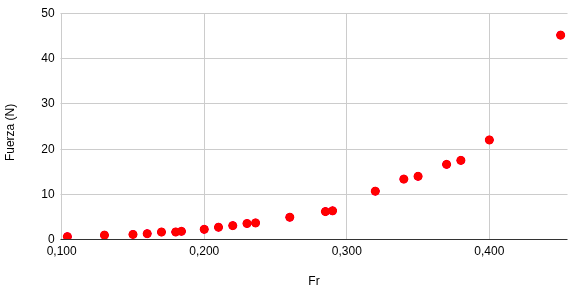
\includegraphics[width=\textwidth]{images/efd-165}
         \caption{Calado 1.}
         \label{fig:resis_tpa_165}
     \end{subfigure}
     \hfill
     \begin{subfigure}[b]{0.45\textwidth}
         \centering
         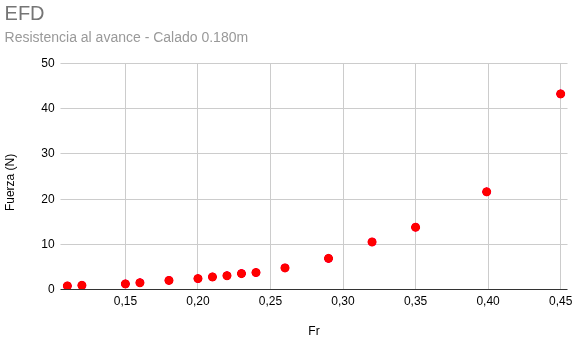
\includegraphics[width=\textwidth]{images/efd-180}
         \caption{Calado 2.}
         \label{fig:resis_tpa_180}
     \end{subfigure}
     
     \vspace{0.5cm} % Espacio entre filas
     
     % --- Segunda fila: Calado 3 centrado ---
     \begin{subfigure}[b]{0.45\textwidth}
         \centering
         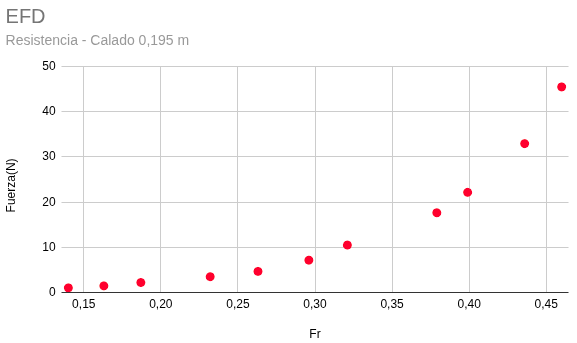
\includegraphics[width=\textwidth]{images/efd-195}
         \caption{Calado 3.}
         \label{fig:resis_tpa_195}
     \end{subfigure}
     
     \caption{Resistencia al avance (EFD) en función de Fr para diferentes calados.}
     \label{fig:comparativa_efd_calados}
\end{figure}


\subsection{Determinación experimental del factor de forma}\label{sec:det_exp_fac_form}

A partir de los resultados experimentales obtenidos para las distintas velocidades y condiciones de calado, se construyeron los diagramas del método de Prohaska, graficando $\frac{C_T}{C_F}$ frente a $\frac{Fr^4}{C_F}$ (Figura~\ref{fig:prohaska_tpa}).  
Cada conjunto de puntos corresponde a un calado diferente del \textit{P1}.  
Según el planteo teórico de \citet{prohaska1966}, los puntos deberían alinearse aproximadamente sobre una recta, cuya extrapolación al origen permite obtener el valor de $(1+k)$.  
Sin embargo, en los tres calados se observa una ligera curvatura en los puntos experimentales, especialmente a bajos números de Froude, lo que indica una desviación del comportamiento lineal esperado.

\begin{figure}[htpb]
\centering
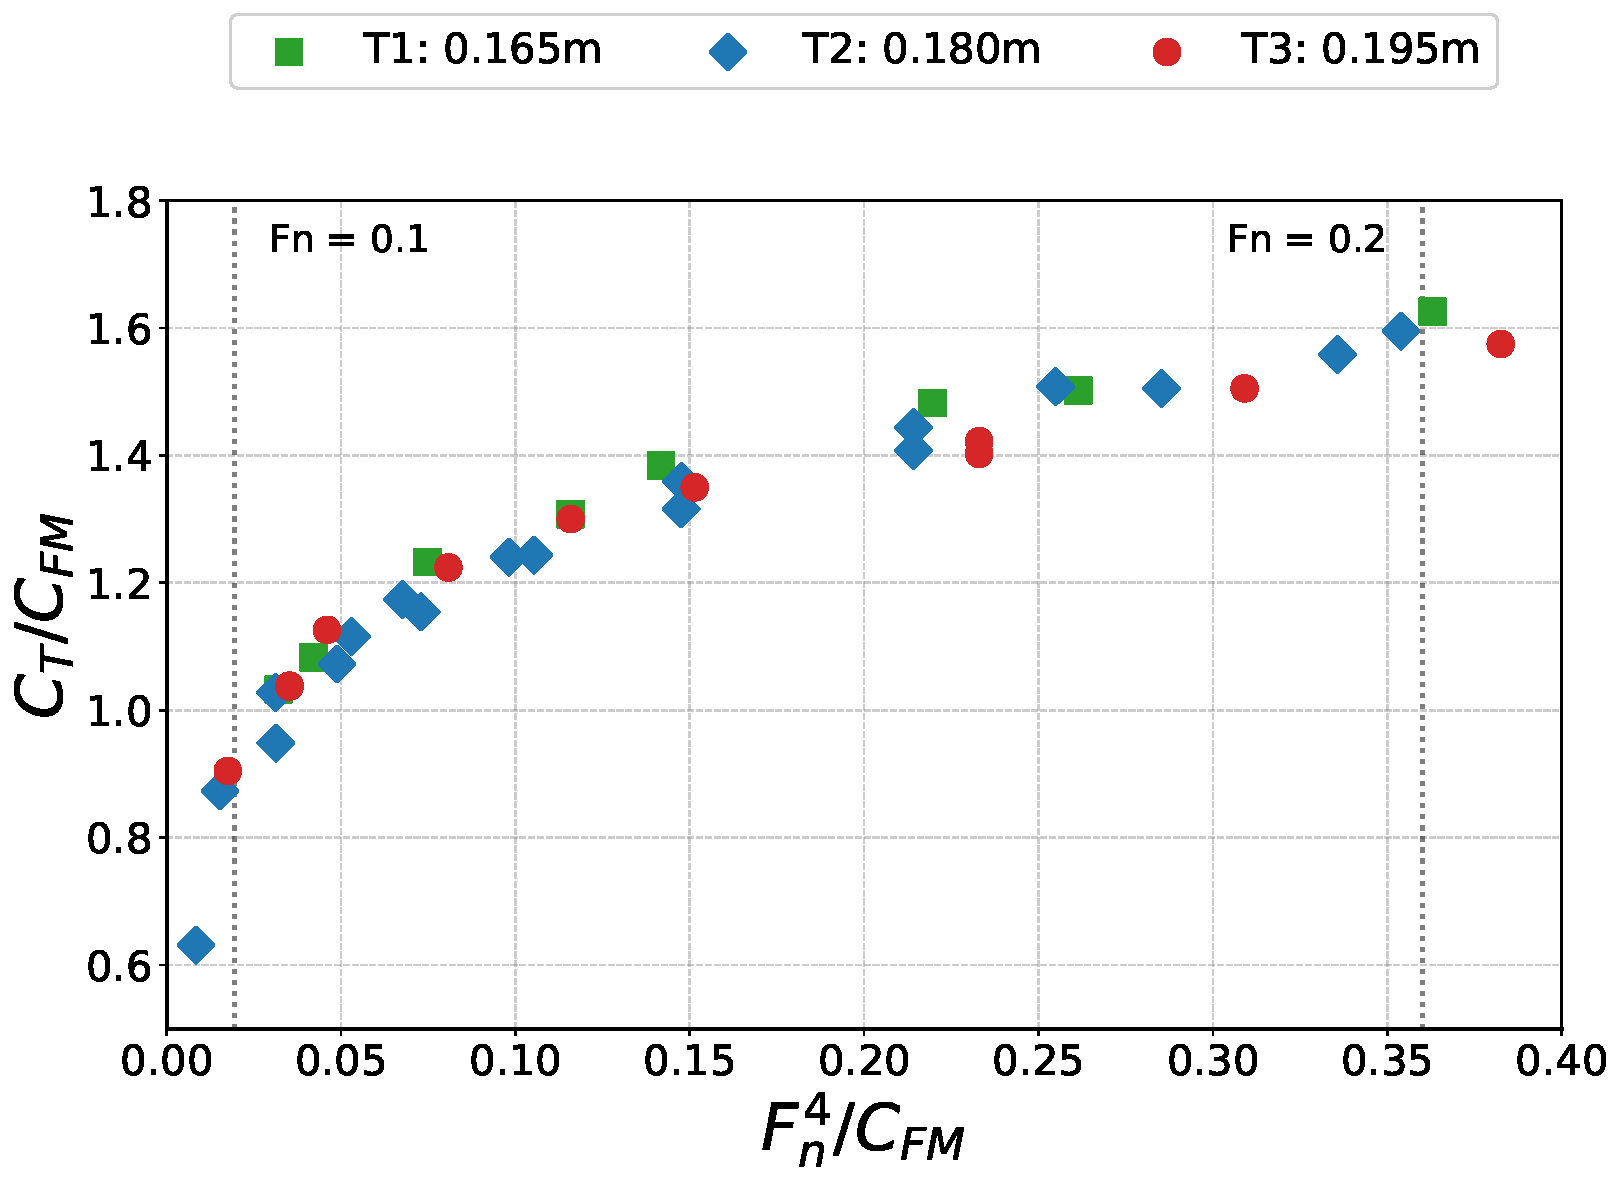
\includegraphics[width=0.6\textwidth]{images/prohaska_tpa_comparacion.pdf}
\caption{Diagramas del método de Prohaska para los tres calados del \textit{P1}. La desviación respecto de la linealidad teórica se acentúa a bajos números de Froude.}
\label{fig:prohaska_tpa}
\end{figure}

Una primera explicación de esta curvatura se relaciona con fenómenos de 
\textit{laminarización} parcial del flujo a bajas velocidades, como se describe 
en \cite{keh-sik-min}. En dichos regímenes, el flujo cercano a la proa puede 
volverse transicional o parcialmente laminar, reduciendo el coeficiente de 
fricción y alterando la pendiente esperada de la curva de Prohaska. A ello se 
suma la elevada sensibilidad del método frente a pequeñas incertidumbres en la 
medición de resistencia total, particularmente cuando el valor absoluto de la 
resistencia es muy bajo. Sin embargo, la laminarización no es la única fuente 
de desviación: como se discute en detalle en la Sección~\ref{sec:prohaska_antec}, 
las causas pueden agruparse en tres categorías: efectos geométricos no lineales 
asociados a la proa bulbo, fenómenos viscosos de separación de flujo en popas 
llenas o espejo sumergido, y curvaturas de naturaleza analítica introducidas 
por la línea de correlación ITTC-1957 o por la aproximación ${\sim}Fr^4$ para 
la resistencia por olas.

Dado que el análisis aplicado al \textit{P1} mostró cierta sensibilidad a los 
puntos considerados en la regresión lineal, se evaluaron distintos rangos de 
Froude para determinar un intervalo robusto. La Figura~\ref{fig:tpa_range} 
muestra, para el Calado~3, el valor de $(1+k)$ obtenido al variar el límite 
inferior del rango de ajuste, manteniendo fijo el límite superior en 
$Fr = 0.20$. Los otros calados presentaron un comportamiento análogo. 
Al eliminar los puntos de $Fr < 0.15$, el valor de $(1+k)$ se estabiliza, 
por lo que se adoptó el rango $0.15 < Fr < 0.20$ como intervalo de aplicación 
del método. Este comportamiento es consistente con la hipótesis de que a bajos 
$Fr$ el flujo presenta mayor proporción laminar o transicional, lo que 
distorsiona la extrapolación. A partir de $Fr \approx 0.15$, la estabilización 
del resultado sugiere que ambas condiciones del método (flujo predominantemente 
turbulento y componente por olas despreciable) se satisfacen de manera más 
razonable, aunque no puede descartarse que otros factores contribuyan a la 
mejora del ajuste.

\begin{figure}[htpb]
    \centering
    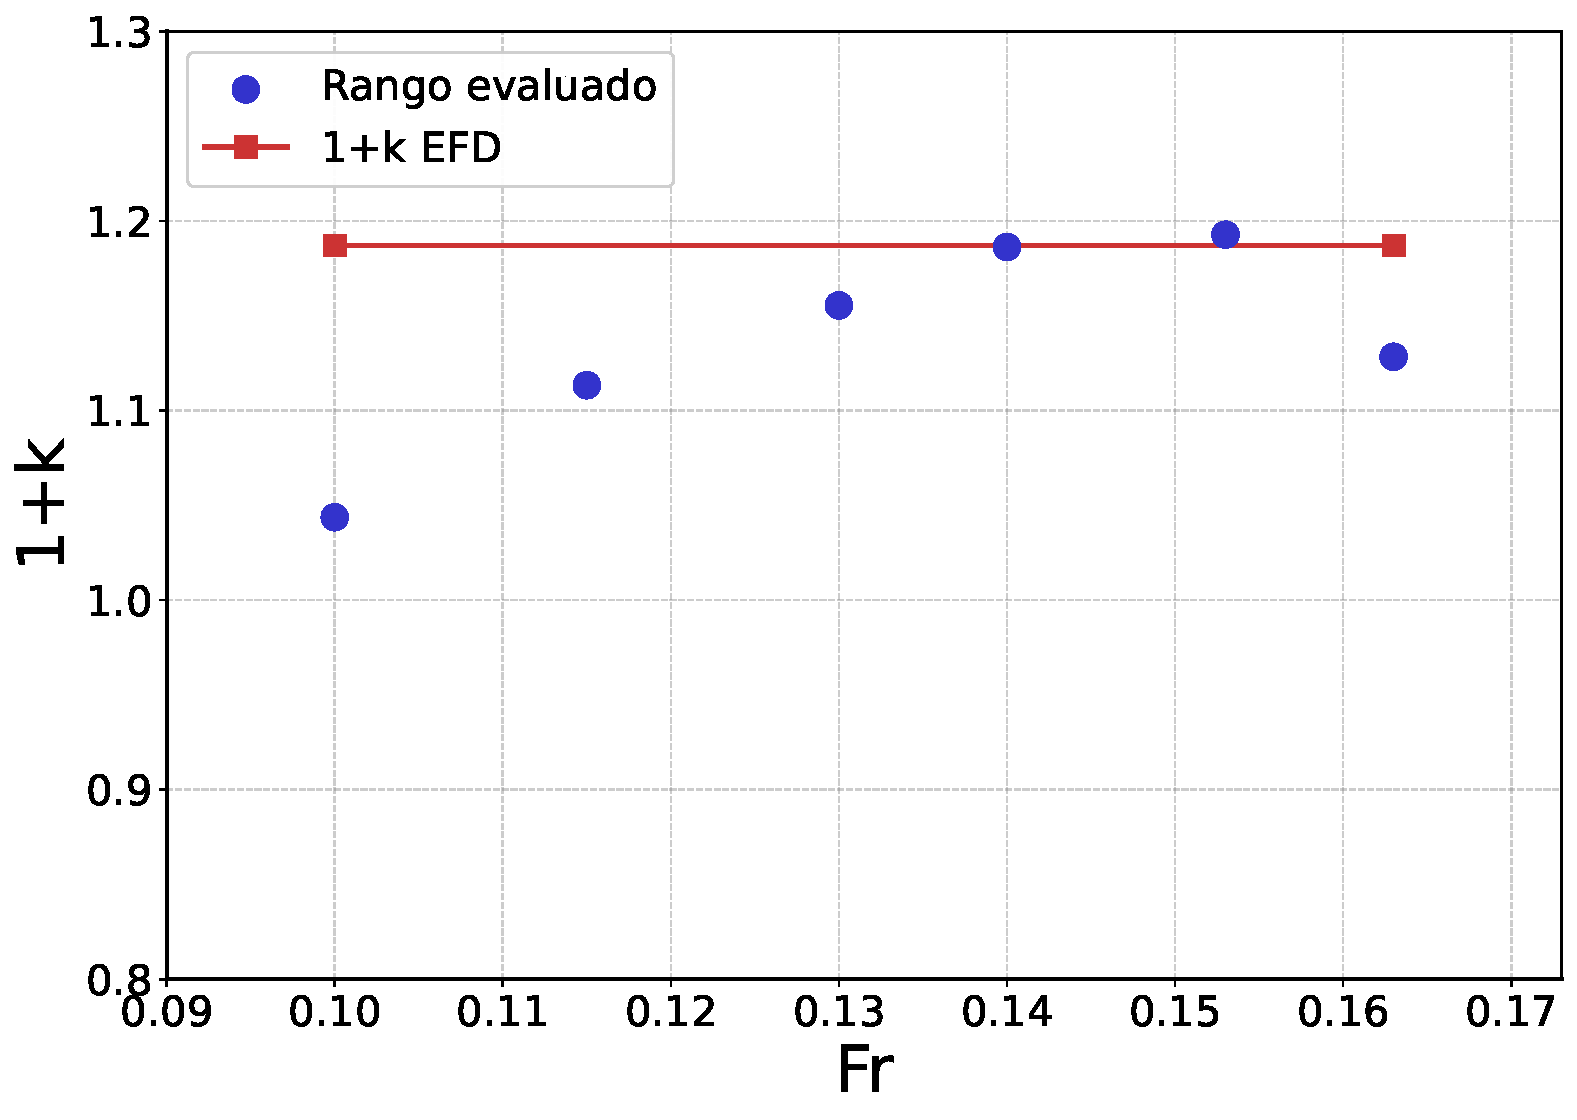
\includegraphics[width=.6\columnwidth]
        {images/efd_form_factor_tpa_range.pdf}
    \caption{Variación del factor de forma $(1+k)$ al modificar el límite 
inferior del rango de Froude (puntos azules), manteniendo el superior 
en $Fr = 0.20$. La línea roja indica el valor de $(1+k)$ adoptado 
mediante el método de Prohaska en el rango $0.15 < Fr < 0.20$. 
Calado~3; comportamiento análogo en otros calados.}
    \label{fig:tpa_range}
\end{figure}

En la Tabla \ref{tab:form_factors} se presenta el factor de forma calculado para cada calado analizado, reduciendo en cada caso el rango de Fr analizado.

\begin{table}[H]
\centering
\caption{Factor de forma $k$ para diferentes calados, calculado mediante el método de Prohaska.}
\begin{tabular}{lccc}
\hline
\textbf{Método} & \textbf{T1: 0.165 m} & \textbf{T2: 0.180 m} & \textbf{T3: 0.195 m} \\
\hline
EFD Prohaska ($k$) & 0.252 & 0.211 & 0.194 \\
\hline
\end{tabular}
\label{tab:form_factors}
\end{table}

Finalmente, para cuantificar la incertidumbre asociada al ajuste lineal, se aplicó el método propuesto por \cite{york}, que considera errores en ambos ejes y proporciona intervalos de confianza para $(1+k)$.  
La Figura~\ref{fig:york_tpa} ilustra un ejemplo del ajuste ponderado obtenido para el Calado 1.  

\begin{figure}[htpb]
\centering
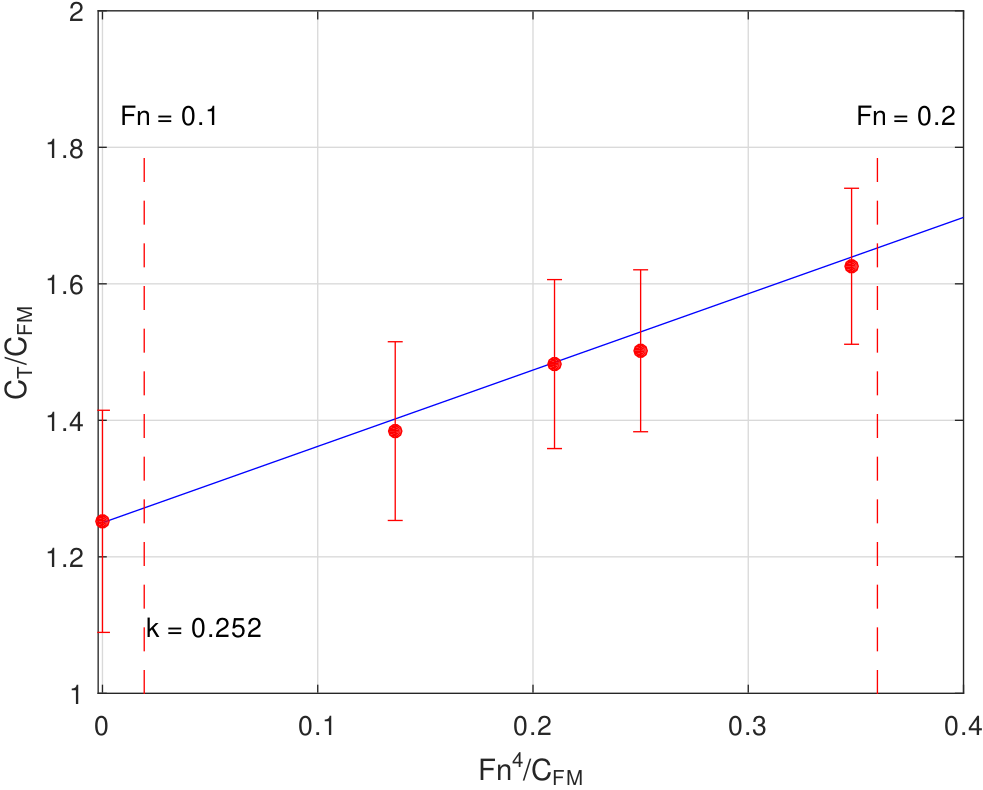
\includegraphics[width=0.6\textwidth]{images/york.png}
\caption{Ajuste lineal con ponderación mediante el método de York aplicado al \textit{P1} para la estimación de $(1+k)$ y su incertidumbre.}
\label{fig:york_tpa}
\end{figure}



En síntesis, las desviaciones observadas responden a causas de distinta 
naturaleza: algunas pueden minimizarse acotando el rango de $Fr$ analizado 
(efectos viscosos por problemas de semejanza con $Re$), otras son inherentes 
al método experimental (incertidumbre en la medición de resistencia total), 
otras son propias de las hipótesis simplificativas del método (línea de 
correlación ITTC-1957, aproximación ${\sim}Fr^4$) y otras son intrínsecas 
a la geometría del casco (proa bulbo, popa espejo sumergida). Estas últimas 
dos categorías se analizan en detalle en las 
Secciones~\ref{sec:proa_bulbo}, \ref{sec:popa_sumergida} 
y \ref{sec:linea_de_friccion}.

\vspace{1em}
\subsubsection{Modelo de referencia KCS}

Con el objetivo de analizar el comportamiento hidrodinámico de un casco 
de referencia y establecer una comparación directa con el \textit{P1}, 
se realizó una segunda campaña experimental utilizando el modelo KCS 
(escala 1:79). Este buque portacontenedores, ampliamente ensayado por 
laboratorios internacionales (KRISO, MARIN, SSPA, Hyundai), satisface 
adecuadamente los supuestos del método de Prohaska y es representativo 
de los cascos para los cuales fue desarrollado: flujo adherido en la 
región de popa, popa espejo sin inmersión significativa y componente de 
olas proporcional a $Fr^4$ en el rango de bajas velocidades. La 
comparación entre ambos cascos permite identificar qué fenómenos 
hidrodinámicos son propios del \textit{P1} y cuáles responden al 
comportamiento esperable para un casco de desplazamiento convencional.

El factor de forma experimental se determinó mediante el método de Prohaska, 
siguiendo el mismo procedimiento de ajuste aplicado al modelo \textit{P1}. 
La Figura~\ref{fig:prohaska_kcs} muestra el diagrama obtenido, donde se 
grafica $C_{TM}/C_{F0}$ frente a $Fr^4/C_{F0}$, siendo $C_{F0}$ el 
coeficiente de fricción de placa plana evaluado al número de Reynolds del 
modelo según la línea ITTC-57. Los puntos experimentales presentan una buena 
alineación sobre la recta de regresión en todo el rango analizado, en 
contraste con el comportamiento observado en el \textit{P1}. Este resultado 
es consistente con lo esperable para un casco como el KCS: la hipótesis de 
Hughes, que sustenta la descomposición de la resistencia viscosa, y la 
aproximación de Prohaska, que supone que la resistencia por olas varía como 
${\sim}Fr^4$, se satisfacen con mayor facilidad cuando el flujo permanece 
adherido y predominantemente turbulento. El KCS opera en un rango de Reynolds 
más elevado que el \textit{P1} ($Re \approx 3.84 \times 10^6$ vs 
$Re \approx 1.60 \times 10^6$ a velocidad de diseño), su proa bulbo opera 
suficientemente alejada de la superficie libre en el rango de $Fr$ analizado, 
y su popa espejo no presenta inmersión significativa, condiciones que en 
conjunto favorecen el cumplimiento de los supuestos del método.

\begin{figure}[htpb]
\centering
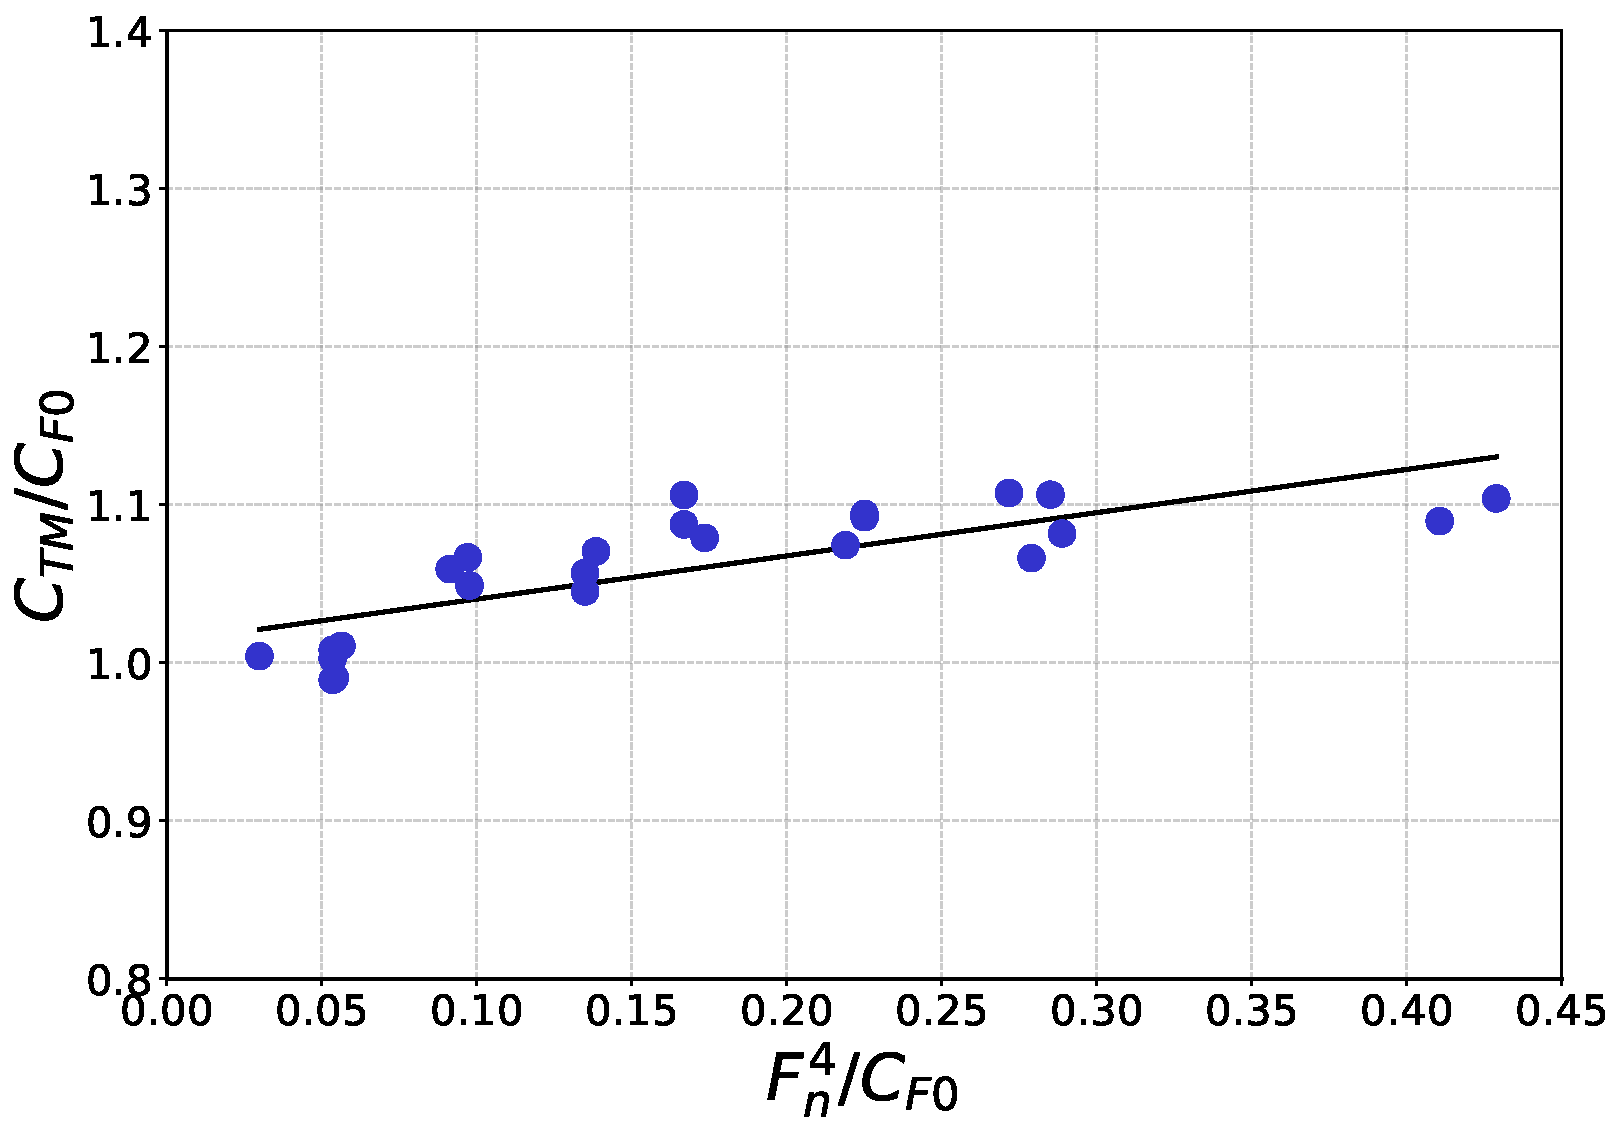
\includegraphics[width=0.6\textwidth]{images/prohaska_kcs.pdf}
\caption{Diagrama de Prohaska para el modelo KCS. Se grafica 
$C_{TM}/C_{F0}$ frente a $Fr^4/C_{F0}$, donde $C_{F0}$ es el 
coeficiente de fricción de placa plana al $Re$ del modelo según 
la línea ITTC-57. La línea continua representa el ajuste por 
mínimos cuadrados, cuya extrapolación al origen permite obtener 
el valor de $1+k$.}
\label{fig:prohaska_kcs}
\end{figure}

Posteriormente se analizó la sensibilidad del resultado al rango de velocidades 
considerado en el ajuste. La Figura~\ref{fig:kcs_range} muestra la evolución 
del valor de $(1+k)$ al variar el límite inferior del rango de $Fr$, 
manteniendo fijo el límite superior en $Fr = 0.20$. A diferencia de lo 
observado en el \textit{P1}, el valor de $(1+k)$ se estabiliza rápidamente, 
con la excepción de los puntos más bajos ($Fr < 0.11$), donde se observa 
una leve caída atribuible a posibles efectos de laminarización. El valor 
adoptado fue $(1+k) = 1.06$, correspondiente al rango $0.13 < Fr < 0.20$.

\begin{figure}[htpb]
\centering
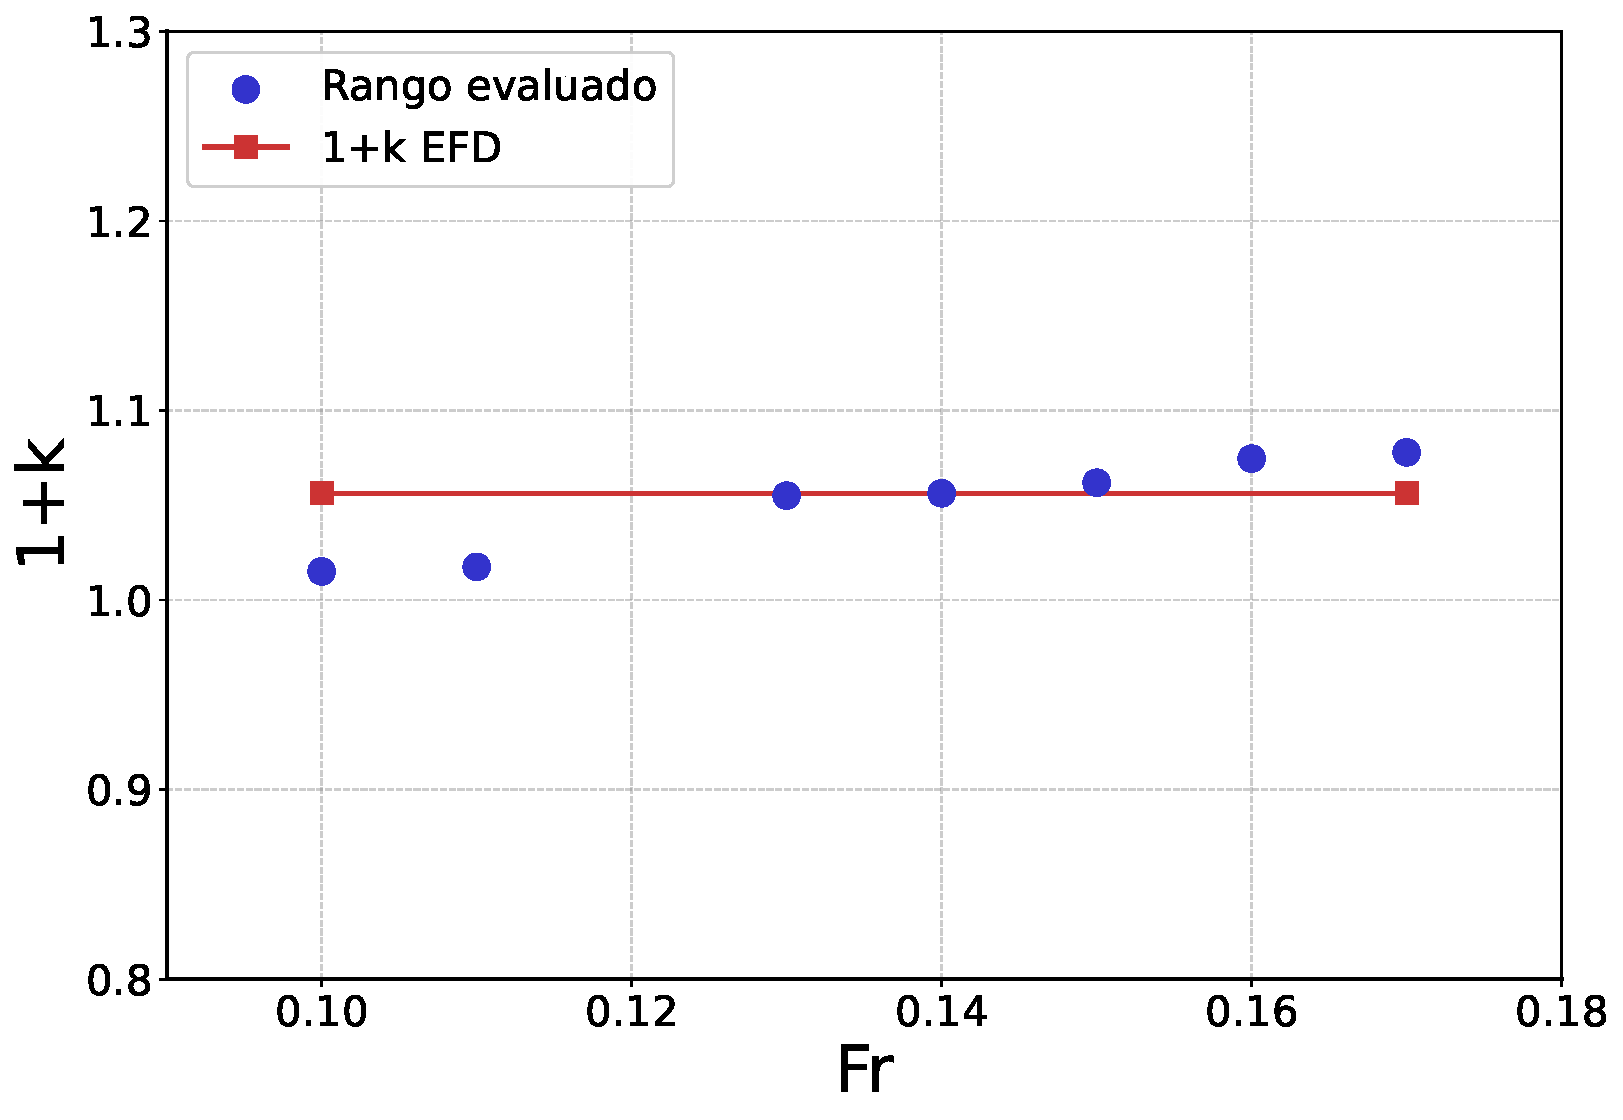
\includegraphics[width=0.6\textwidth]{images/efd_form_factor_kcs_range.pdf}
\caption{Variación del factor de forma $(1+k)$ para el modelo KCS en función 
del límite inferior del rango de Froude utilizado en el ajuste de Prohaska, 
con límite superior fijo en $Fr = 0.20$. El cuadrado rojo indica el valor 
adoptado.}
\label{fig:kcs_range}
\end{figure}

Finalmente, la Figura~\ref{fig:kcs_validation} compara el valor obtenido en 
el LabHiNO con los recopilados por \citet{TerzievDataSet} a partir de ensayos 
de distintos laboratorios internacionales. El punto del LabHiNO se ubica en 
la zona de crecimiento de $(1+k)$ con $Re$, en perfecta concordancia con la 
tendencia general de los datos de referencia, confirmando que el canal 
reproduce correctamente el comportamiento esperado para este casco a la escala 
ensayada.

\begin{figure}[htpb]
\centering
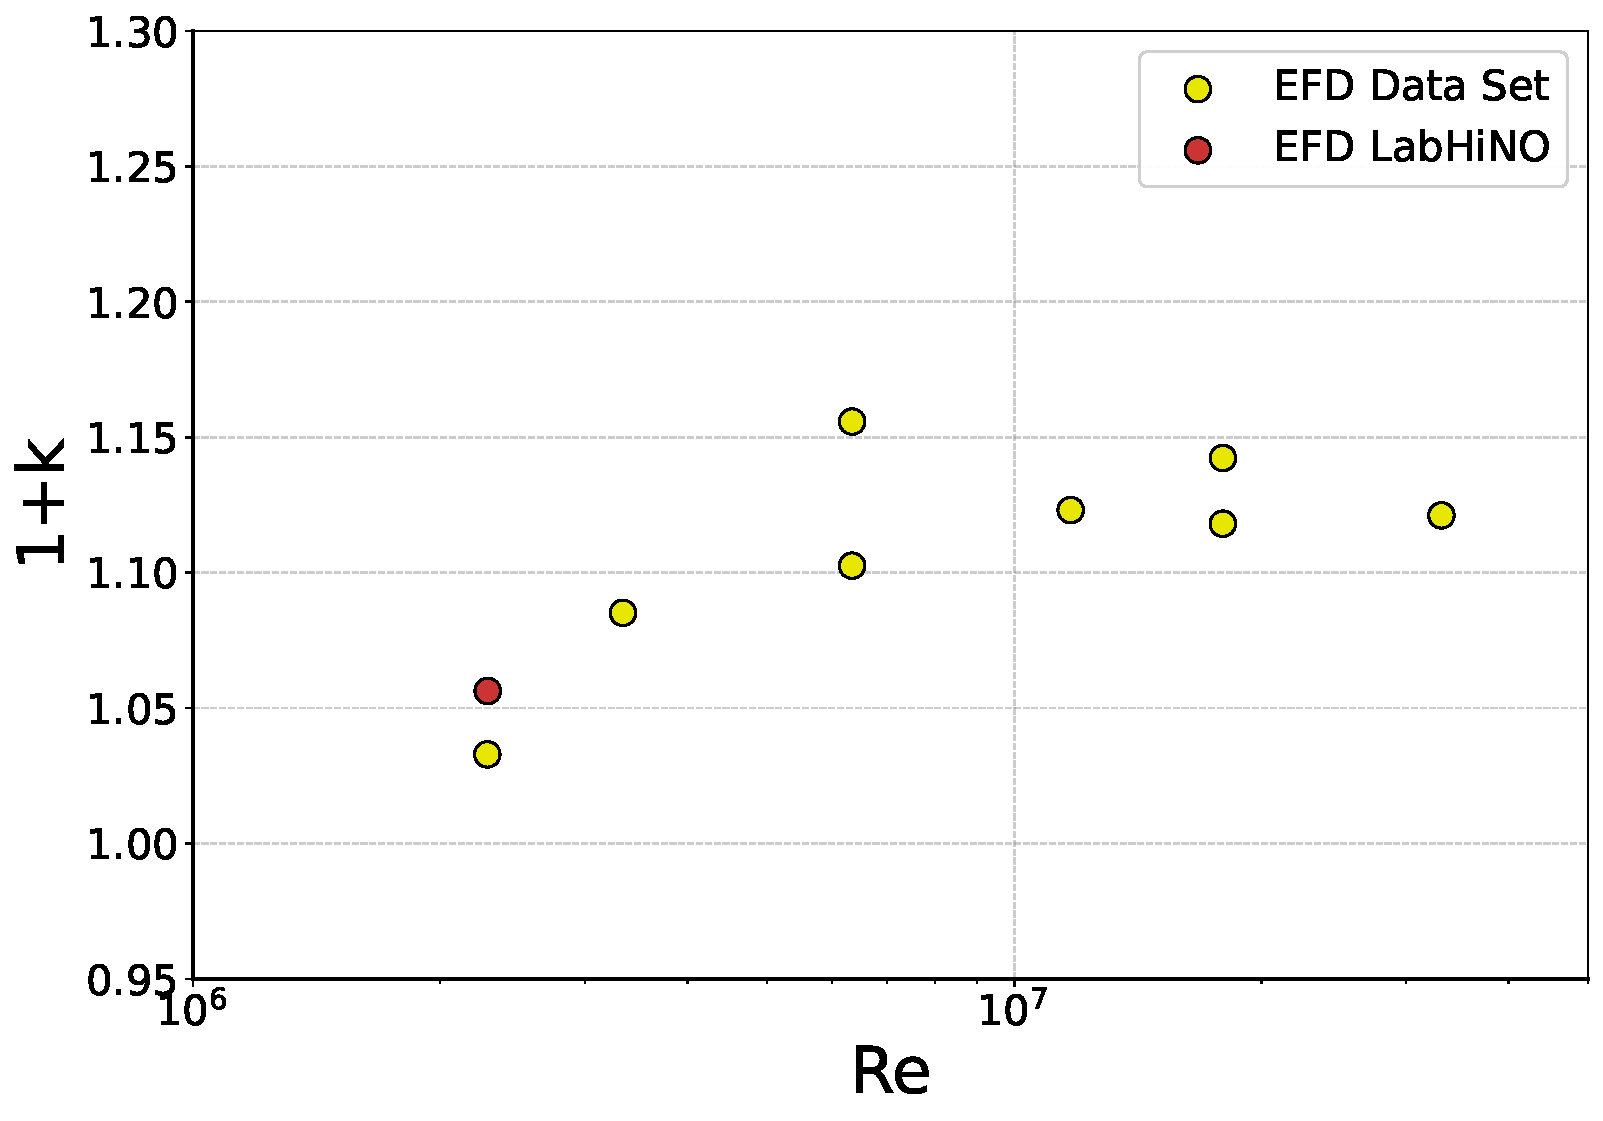
\includegraphics[width=0.6\textwidth]{images/efd_kcs_lit.pdf}
\caption{Comparación del factor de forma $(1+k)$ del KCS obtenido en el 
LabHiNO (punto rojo) con resultados experimentales históricos del KCS 
compilados de literatura internacional por \citet{TerzievDataSet} 
(puntos amarillos), en función del número de Reynolds.}
\label{fig:kcs_validation}
\end{figure}


\subsection{Ensayos computacionales de resistencia al avance}

Con el objetivo de validar la herramienta numérica y descomponer la resistencia 
total en sus componentes físicas, se replicaron computacionalmente los ensayos 
de canal descritos en la sección anterior. Las simulaciones se realizaron 
siguiendo la configuración metodológica detallada en el Capítulo~\ref{chap:Metodologia}, 
utilizando el solucionador multifásico \texttt{interFoam} para capturar la 
deformación de la superficie libre.

El dominio computacional, Figura~\ref{fig:dominio_metodologia}, reproduce las condiciones de aguas 
profundas del canal, asegurando también que las reflexiones de olas en los 
límites laterales no interfieran con la medición de resistencia en el casco. 
Las condiciones de contorno empleadas corresponden al esquema estándar 
presentado en la Tabla~\ref{tab:bc_setup}, garantizando la conservación de 
masa y la correcta generación de turbulencia en la capa límite mediante el 
modelo $k$-$\omega$ SST.

A diferencia del ensayo experimental, donde solo se obtiene la fuerza integral 
$R_{TM}$, el enfoque numérico permite separar las contribuciones de las fuerzas 
de presión y de fricción. Esta descomposición es fundamental para analizar la 
influencia de la forma del casco en la resistencia viscosa, aspecto que se 
discute en las secciones siguientes.

La validación del modelo numérico frente a los ensayos experimentales constituye 
un paso previo indispensable antes de proceder al análisis mediante el método de 
doble cuerpo. A diferencia de las simulaciones bifásicas con superficie libre, 
cuyas predicciones de resistencia total pueden cotejarse directamente con los 
resultados EFD, las simulaciones de doble cuerpo no tienen una contrapartida 
experimental directa: al eliminar la superficie libre se suprime también la 
componente de resistencia por olas, lo que imposibilita una comparación global 
con el ensayo de canal. Por este motivo, la confianza en los resultados del 
doble cuerpo descansa en la validación previa del modelo numérico completo. 
La concordancia entre EFD y CFD bifásico presentada en las 
Figuras~\ref{fig:resis_tpa_efd_cfd_165} a~\ref{fig:resis_tpa_efd_cfd_195} 
confirma que la configuración numérica, dominio, malla, modelo de turbulencia 
y condiciones de contorno, reproduce correctamente la física del problema, 
lo que respalda la confiabilidad de las simulaciones de doble cuerpo 
presentadas en la sección siguiente.

En la Figura~\ref{fig:3D-comparacion} se presenta una comparación del patrón 
de olas sobre el casco del \textit{P1} obtenido con el modelo CFD y el ensayo 
experimental (EFD), para el Calado~3 a tres números de Froude distintos 
($Fr = 0.26$, $0.37$ y $0.45$). Los tres casos ilustran la capacidad del 
modelo numérico para reproducir el patrón de olas generado por el buque en 
diferentes condiciones de velocidad.

\begin{figure}[H]
    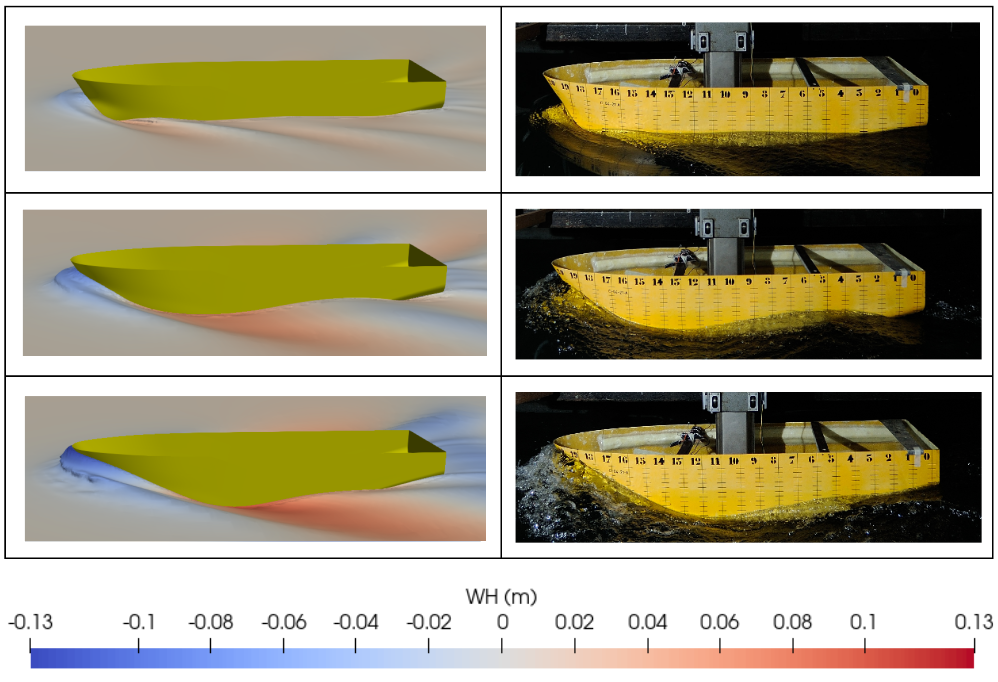
\includegraphics[width=1\linewidth]{images/3D-comparacion1.png}
    \caption{Patrón de olas sobre el \textit{P1} para distintos $Fr$ y 
    Calado~3. \textbf{Columna izquierda}: modelo CFD. 
    \textbf{Columna derecha}: EFD. 
    \textbf{Primera fila}: $Fr = 0.26$; \textbf{segunda fila}: $Fr = 0.37$; 
    \textbf{tercera fila}: $Fr = 0.45$.}
    \label{fig:3D-comparacion}
\end{figure}

En las Figuras~\ref{fig:cfd_165_tpa} a~\ref{fig:cfd_195_tpa} se presentan 
las curvas de resistencia total obtenidas para los tres calados del 
\textit{P1}. En todos los casos se observa un incremento continuo de la 
resistencia con el número de Froude, mostrando la transición habitual entre 
el régimen de bajas velocidades, donde la contribución viscosa domina el 
comportamiento global, y el rango a partir de $Fr \approx 0.30$, donde la 
componente asociada a la generación de olas comienza a desarrollarse con mayor 
intensidad. La evolución suave de las curvas y la ausencia de oscilaciones 
significativas indican que las simulaciones convergen de forma estable hacia 
un régimen estacionario, reproduciendo adecuadamente el comportamiento 
esperado para un ensayo de remolque.

\begin{figure}[htpb]
     \centering
     \begin{subfigure}[b]{0.45\textwidth}
         \centering
         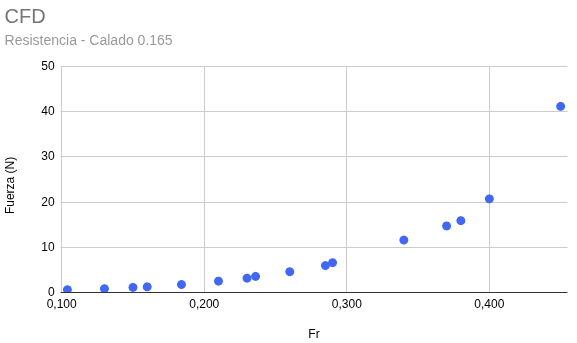
\includegraphics[width=\textwidth]{images/cfd-165}
         \caption{Calado 1.}
         \label{fig:cfd_165_tpa}
     \end{subfigure}
     \hfill
     \begin{subfigure}[b]{0.45\textwidth}
         \centering
         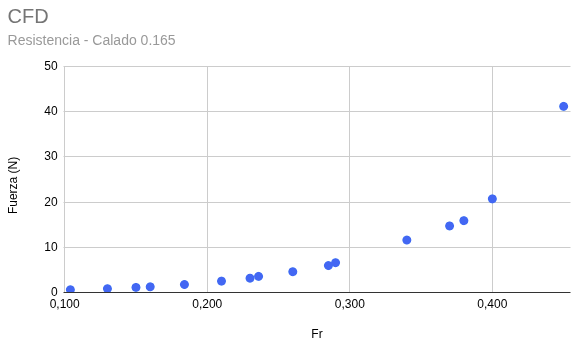
\includegraphics[width=\textwidth]{images/cfd-180}
         \caption{Calado 2.}
         \label{fig:cfd_180_tpa}
     \end{subfigure}
     
     \vspace{0.5cm}
     
     \begin{subfigure}[b]{0.45\textwidth}
         \centering
         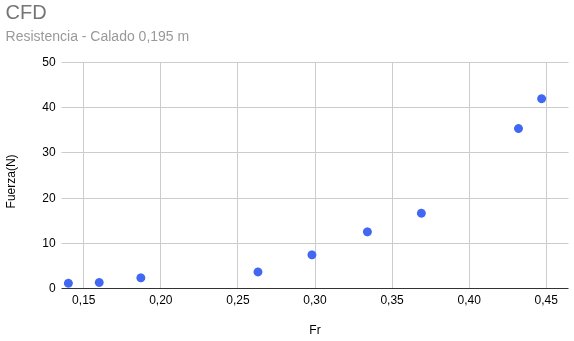
\includegraphics[width=\textwidth]{images/cfd-195}
         \caption{Calado 3.}
         \label{fig:cfd_195_tpa}
     \end{subfigure}
     
     \caption{Resistencia al avance del \textit{P1} obtenida por CFD en 
     función de $Fr$ para los tres calados.}
     \label{fig:comparativa_calados}
\end{figure}


\subsection{Determinación numérica del factor de forma}\label{sec:det_num_fac_form}

Para la determinación computacional del factor de forma se implementaron dos métodos. El primero fue repetir lo propuesto por Prohaska para lo tres calados con el dominio presentado en la Figura \ref{fig:dominio_metodologia}, mientras que el segundo, que será tratado en detalle en la Sección \ref{sec:4.1.5_enfoque_doble_cuerpo}, implica la simulación únicamente de la obra viva eliminando la superficie libre. El primer método permite una comparación directa con el ensayo experimental. Como sucedió en los ensayos experimentales, a bajas velocidades también se observa en los ensayos CFD una separación de los puntos respecto de la recta teórica esperada, pero esta vez de forma cóncava en lugar de convexa, como se ve en la Figura \ref{fig:prohaska_tpa_cfd}.


\begin{figure}[htpb]
\centering
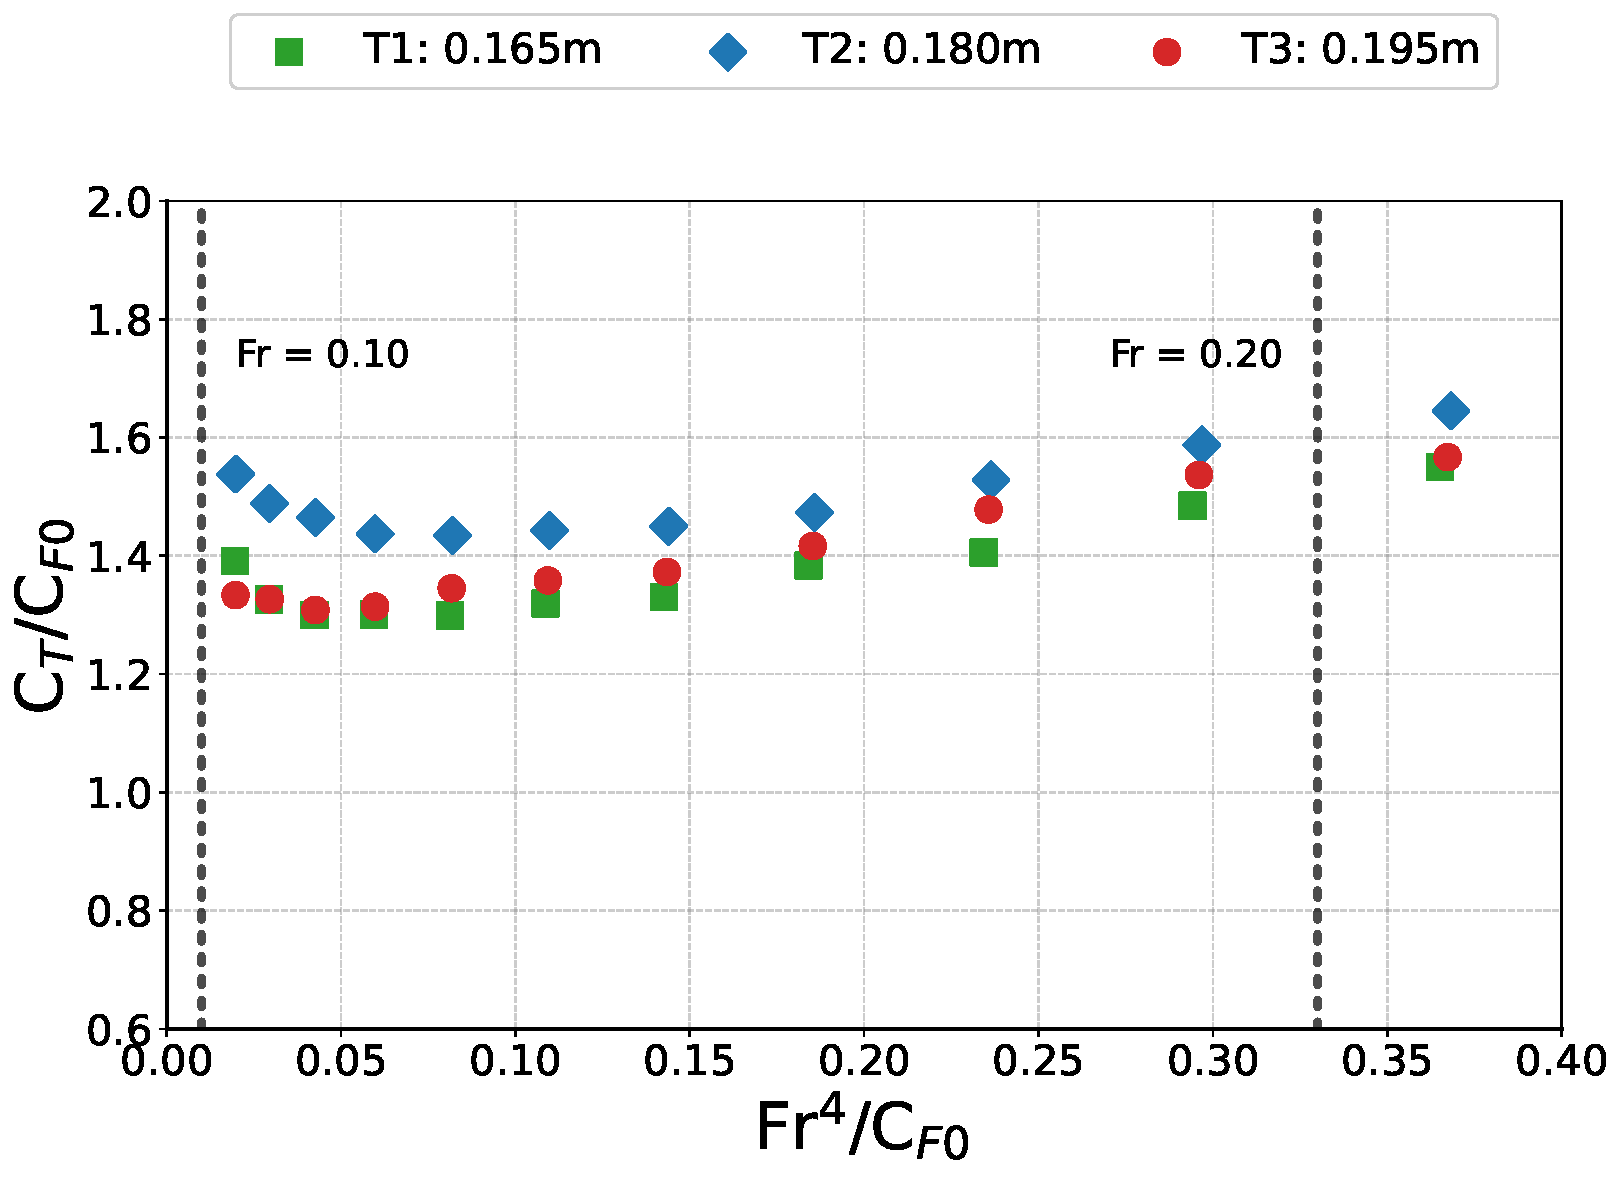
\includegraphics[width=0.6\textwidth]{images/prohaska_tpa_cfd_comparacion.pdf}
\caption{Diagramas del método de Prohaska para los tres calados del \textit{P1}. La desviación respecto de la linealidad teórica se acentúa a bajos números de Froude.}
\label{fig:prohaska_tpa_cfd}
\end{figure}

La diferencia observada a bajas velocidades sugiere una deficiencia en el modelado de la zona de transición. Dado que el modelo $k-\omega$ SST asume un régimen turbulento, carece de la sensibilidad necesaria para capturar correctamente la transición de la capa límite en las simulaciones. El punto de transición suele verse adelantado por los modelos que asumen flujo turbulento. 

Al igual que se hizo con los ensayos experimentales, se repite el análisis de rangos de Froude para el análisis computacional del factor de forma. Dado que los tres calados presentaron un comportamiento análogo, tanto en la 
forma de la curva como en la sensibilidad al rango de Froude considerado, 
presentar los resultados de cada uno por separado no aportaría información 
adicional sino que recargaría innecesariamente la exposición. Por este motivo, 
de aquí en adelante el análisis se centra en el Calado~3, que corresponde a la 
condición de plena carga y resulta el más representativo del régimen de operación del \textit{P1}. La Figura~\ref{fig:tpa_range_cfd} muestra la variación de $(1+k)$ en función del límite inferior del rango de Froude utilizado en el ajuste de Prohaska, con límite superior fijo en $Fr = 0.20$, junto con el valor adoptado como representativo del factor de forma para este calado.

\begin{figure}[htpb]
	\centering
	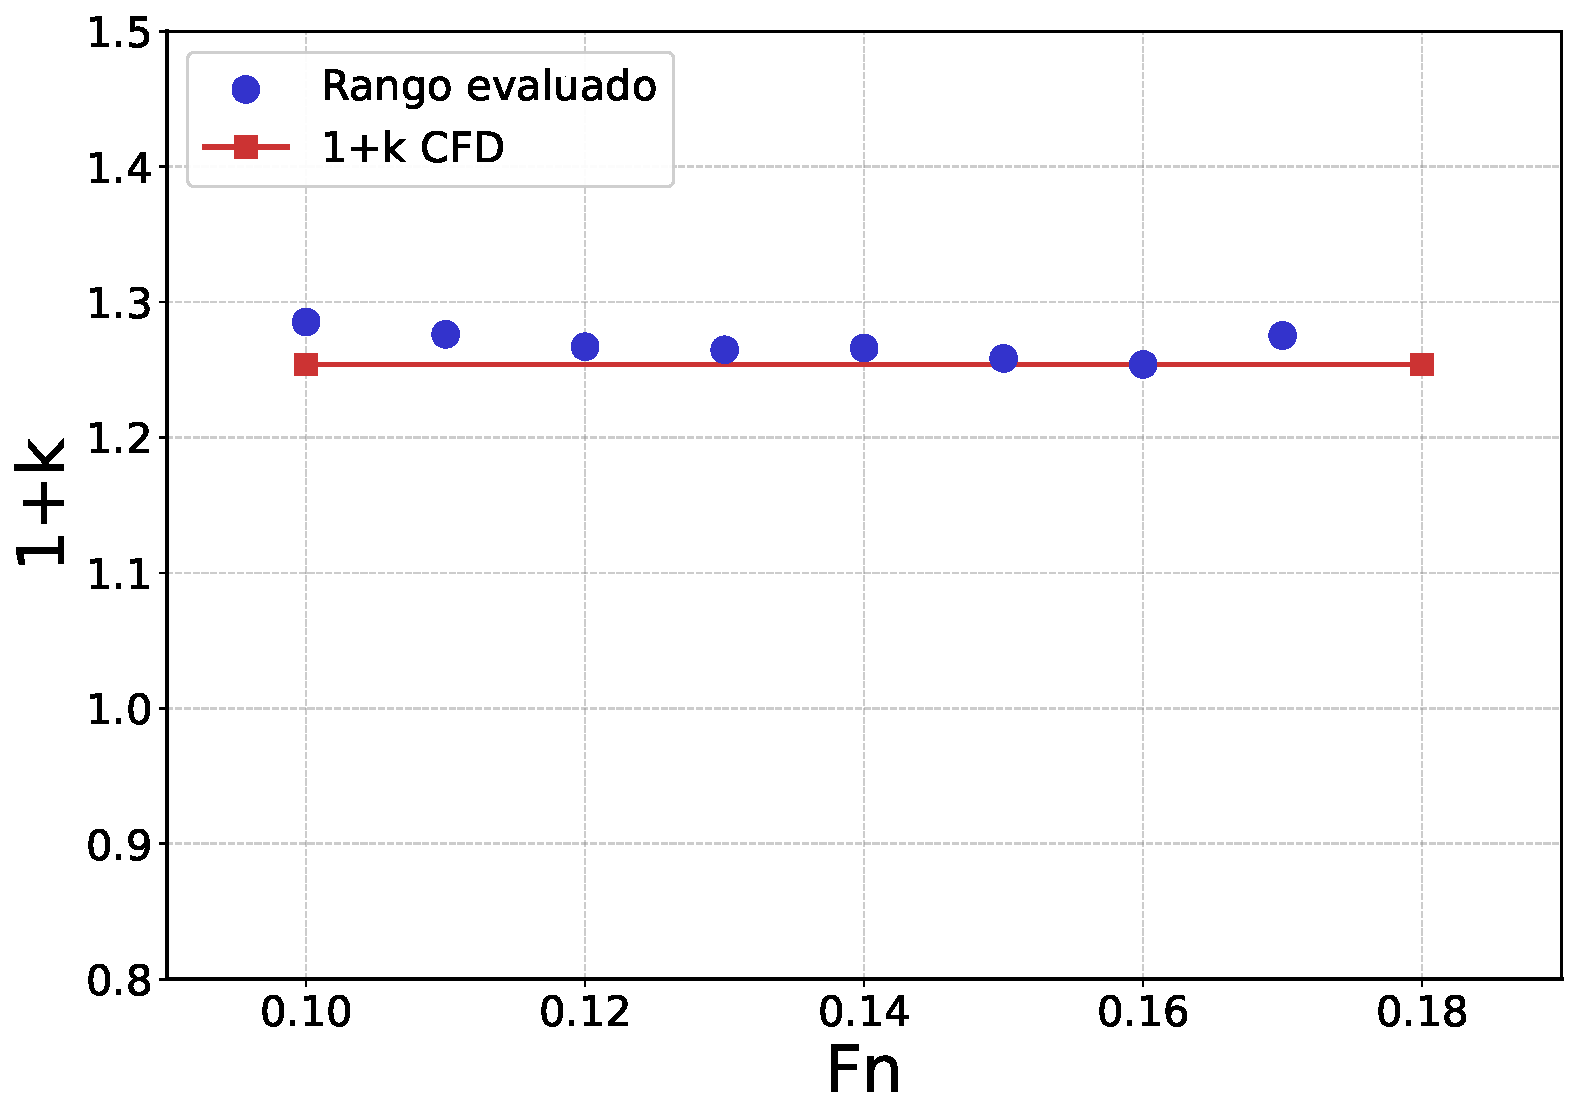
\includegraphics[width=.6\columnwidth]{images/cfd_form_factor_tpa_195_range.pdf}
	\caption{Variación del factor de forma experimental $(1+k)$ para el \textit{P1} en función del rango de Froude utilizado en el ajuste de Prohaska. Calado 3}
\label{fig:tpa_range_cfd}
\end{figure}

\subsection{Enfoque de Doble Cuerpo}\label{sec:4.1.5_enfoque_doble_cuerpo}

Ante las dificultades observadas para aplicar el método de Prohaska en el 
entorno numérico, debido a la incertidumbre en la transición de la turbulencia 
y la curvatura observada en el diagrama $C_{TM}/C_{F0}$ vs $Fr^4/C_{F0}$ a 
bajas velocidades, se optó por una estrategia alternativa: el método de 
\textit{doble cuerpo}, descripto en la Sección~\ref{sec:doble_cuerpo}.

Como se detalló en la Sección \ref{sec:doble_cuerpo}, este enfoque elimina la superficie libre y la formación de olas, modelando el fluido como un medio infinito y el casco como un cuerpo reflejado (ver Figura \ref{fig:double_body_domain}). Esto permite aislar la resistencia viscosa ($R_V$) y calcular el factor de forma $(1+k)$ directamente para cada velocidad mediante la relación $C_V / C_{F0}$, sin depender de la extrapolación a velocidad cero.

\subsubsection{Análisis del \textit{P1}}


Antes de interpretar el comportamiento físico del factor de forma, se
verifica la fiabilidad numérica de las simulaciones en las cuatro escalas
geométricas. La Tabla~\ref{tab:CFD_summary_compact} resume, para cada número
de Froude, el número de Reynolds, la resolución de pared ($y^+$), el factor de
forma $(1+k)$ y el índice de convergencia de malla (GCI).

\begin{table}[htbp]
\centering
\caption{Resumen de las simulaciones CFD para las cuatro escalas geométricas
del \textit{P1} (Calado~3): número de Reynolds, resolución de pared ($y^+$),
factor de forma $(1+k)$ e índice de convergencia de malla (GCI) para cada
número de Froude. Modelo de turbulencia: $k$--$\omega$ SST.}
\label{tab:CFD_summary_compact}
\footnotesize
\begin{tabularx}{\textwidth}{>{\bfseries}c *{4}{>{\centering\arraybackslash}X}}
\toprule
\textbf{Fr} & \textbf{1:20} & \textbf{1:10} & \textbf{1:5} & \textbf{1:1} \\
\midrule
\multicolumn{5}{c}{\textbf{Número de Reynolds}} \\[-0.3em]
\multicolumn{5}{c}{\rule{\dimexpr\textwidth-2\tabcolsep}{0.2pt}} \\[0.4em]
\textbf{0.100} & $6.40\times10^{5}$ & $1.81\times10^{6}$ & $5.12\times10^{6}$ & $5.73\times10^{7}$ \\
\textbf{0.160} & $1.02\times10^{6}$ & $2.90\times10^{6}$ & $8.20\times10^{6}$ & $9.17\times10^{7}$ \\
\textbf{0.200} & $1.28\times10^{6}$ & $3.62\times10^{6}$ & $1.02\times10^{7}$ & $1.15\times10^{8}$ \\
\textbf{0.240} & $1.54\times10^{6}$ & $4.35\times10^{6}$ & $1.23\times10^{7}$ & $1.37\times10^{8}$ \\
\textbf{0.300} & $1.92\times10^{6}$ & $5.43\times10^{6}$ & $1.54\times10^{7}$ & $1.72\times10^{8}$ \\
\textbf{0.360} & $2.31\times10^{6}$ & $6.52\times10^{6}$ & $1.84\times10^{7}$ & $2.06\times10^{8}$ \\
\textbf{0.400} & $2.56\times10^{6}$ & $7.25\times10^{6}$ & $2.05\times10^{7}$ & $2.29\times10^{8}$ \\
\midrule
\multicolumn{5}{c}{\textbf{Resolución de pared ($y^+$)}} \\[-0.3em]
\multicolumn{5}{c}{\rule{\dimexpr\textwidth-2\tabcolsep}{0.2pt}} \\[0.4em]
\textbf{0.100} & 0.40 & 8.42$^{c}$ & 12.0 & 108 \\
\textbf{0.160} & 0.70 & 9.00 & 17.0 & 168 \\
\textbf{0.200} & 1.03 & 11.0 & 22.0 & 207 \\
\textbf{0.240} & 1.40 & 11.4 & 26.0 & 245 \\
\textbf{0.300} & 2.23 & 12.6 & 32.0 & 302 \\
\textbf{0.360} & 2.70 & 14.6 & 38.0 & 353 \\
\textbf{0.400} & 3.00 & 15.9 & 41.0 & 389 \\
\midrule
\multicolumn{5}{c}{\textbf{Factor de forma $(1+k)$}} \\[-0.3em]
\multicolumn{5}{c}{\rule{\dimexpr\textwidth-2\tabcolsep}{0.2pt}} \\[0.4em]
\textbf{0.100} & 1.179 & 1.399 & 1.489 & 1.654 \\
\textbf{0.160} & 1.251 & 1.622$^{b}$ & 1.484 & 1.690 \\
\textbf{0.200} & 1.320 & 1.570 & 1.501 & 1.713 \\
\textbf{0.240} & 1.378 & 1.513 & 1.522 & 1.714 \\
\textbf{0.300} & 1.470 & 1.465 & 1.528 & 1.727 \\
\textbf{0.360} & 1.598 & 1.465 & 1.548 & 1.731 \\
\textbf{0.400} & 1.637 & 1.473 & 1.554 & 1.745 \\
\midrule
\multicolumn{5}{c}{\textbf{Índice de convergencia de malla (GCI) [\%]}} \\[-0.3em]
\multicolumn{5}{c}{\rule{\dimexpr\textwidth-2\tabcolsep}{0.2pt}} \\[0.4em]
\textbf{0.100} & 0.028 & 0.773 & 1.748 & 0.002 \\
\textbf{0.160} & 0.112 & 1.032 & 0.005 & 0.849 \\
\textbf{0.200} & 0.009 & 3.722 & 0.859 & 3.730 \\
\textbf{0.240} & 0.003 & 2.193 & 0.723 & 3.985 \\
\textbf{0.300} & 0.002 & 0.001 & 3.544 & 1.681 \\
\textbf{0.360} & 1.382 & 0.003 & 0.311 & 2.053 \\
\textbf{0.400} & 13.433$^{a}$ & 0.011 & 0.090 & 4.421 \\
\bottomrule
\end{tabularx}

\vspace{0.4em}
{\footnotesize\raggedright
$^{a}$~El punto 1:20 / $Fr = 0{.}400$ presenta $GCI = 13{.}4\%$, atribuible a
la complejidad del campo de flujo a alta velocidad; esta condición queda fuera
del rango operativo del buque ($Fr \lesssim 0{.}36$) y no se considera en el
análisis de efectos de escala.\\
$^{b}$~El valor $1+k = 1{.}622$ en 1:10 / $Fr = 0{.}160$ ($y^+ = 9{.}0$) se
aparta de la tendencia de su columna; su ubicación en la región
\textit{buffer}, por debajo del umbral de conmutación de la función de pared,
sugiere un origen numérico asociado al tratamiento de pared más que físico.\par}
\end{table}

Dado que las cuatro escalas geométricas se simularon con mallas
geométricamente similares, la distancia media a la pared en unidades de pared
crece con el número de Reynolds: desde $y^+ \sim 1$ en la menor escala de
modelo hasta $y^+ > 300$ en escala buque. La escala 1:20 resuelve la subcapa
viscosa ($y^+ \lesssim 5$), mientras que las mallas de escala buque ubican el
primer centro de celda dentro de la capa logarítmica
($30 \lesssim y^+ \lesssim 300$), rango de operación previsto para el enfoque
de funciones de pared. Las dos escalas intermedias (1:10 y 1:5) se sitúan
mayormente en la región \textit{buffer} ($5 \lesssim y^+ \lesssim 30$). En
esta región, la formulación de $\omega$ empleada por el modelo $k$--$\omega$
SST combina de forma continua las expresiones viscosa y logarítmica
\citep{Menter1994}, lo que le confiere una relativa insensibilidad a la
posición de la primera celda; no obstante, la región \textit{buffer}
constituye el régimen de menor fiabilidad para el tratamiento de pared, por lo
que las escalas intermedias deben interpretarse con mayor cautela que las
escalas resuelta y de capa logarítmica.

Esta menor fiabilidad se refleja en la dispersión local del factor de forma:
en las escalas intermedias, los valores de $(1+k)$ varían de manera no
monótona con la velocidad y alcanzan índices de convergencia de malla de hasta
aproximadamente un 4\%, en consistencia con la mayor incertidumbre numérica de
la componente de presión viscosa reportada para las simulaciones de doble
cuerpo \citep{KORKMAZ2022112590}. Los resultados de escala buque, que son los
que sustentan las conclusiones de esta tesis, resultan en cambio suaves y
monótonos con el número de Reynolds ($1+k$ crece de $1{.}654$ a $1{.}745$ en el
rango analizado), se ubican en el rango de $y^+$ válido para las funciones de
pared y no presentan cambios de pendiente ni anomalías. La tendencia de
$(1+k)$ a crecer con $Re$ sin alcanzar un valor asintótico es, por lo tanto,
robusta: se sostiene tanto en la escala buque, resuelta en un régimen de pared
adecuado, como en la consistencia global de la curva, aun cuando algunos
puntos individuales de la región \textit{buffer} se dispersen en torno a ella.

La Figura \ref{fig:tpa_DB_k_evolucion} muestra la distribución del factor de forma calculado para los tres calados analizados empleando la configuración de malla verificada en la Sección~\ref{sec:convergencia_de_malla}. Contrario a la hipótesis clásica de la ITTC, que asume un factor de forma constante e independiente de la velocidad ($k \neq f(Fr, Re)$), los resultados obtenidos revelan una variación significativa y sistemática de $(1+k)$ a lo largo del rango de Froude evaluado.

Este hallazgo resulta crítico: si el factor de forma varía de manera apreciable dentro de la misma escala, la selección de un valor único para el proceso de extrapolación a escala buque se vuelve inherentemente ambigua. Más aún, la tendencia creciente observada sugiere una fuerte dependencia con el número de Reynolds, una problemática de efectos de escala que se abordará en profundidad en la Sección \ref{sec:analisis_efectos_escala}.

\begin{figure}[htpb]
    \centering
    % Primera fila: Calado 1 y Calado 2
    \begin{subfigure}[b]{0.48\textwidth}
        \centering
        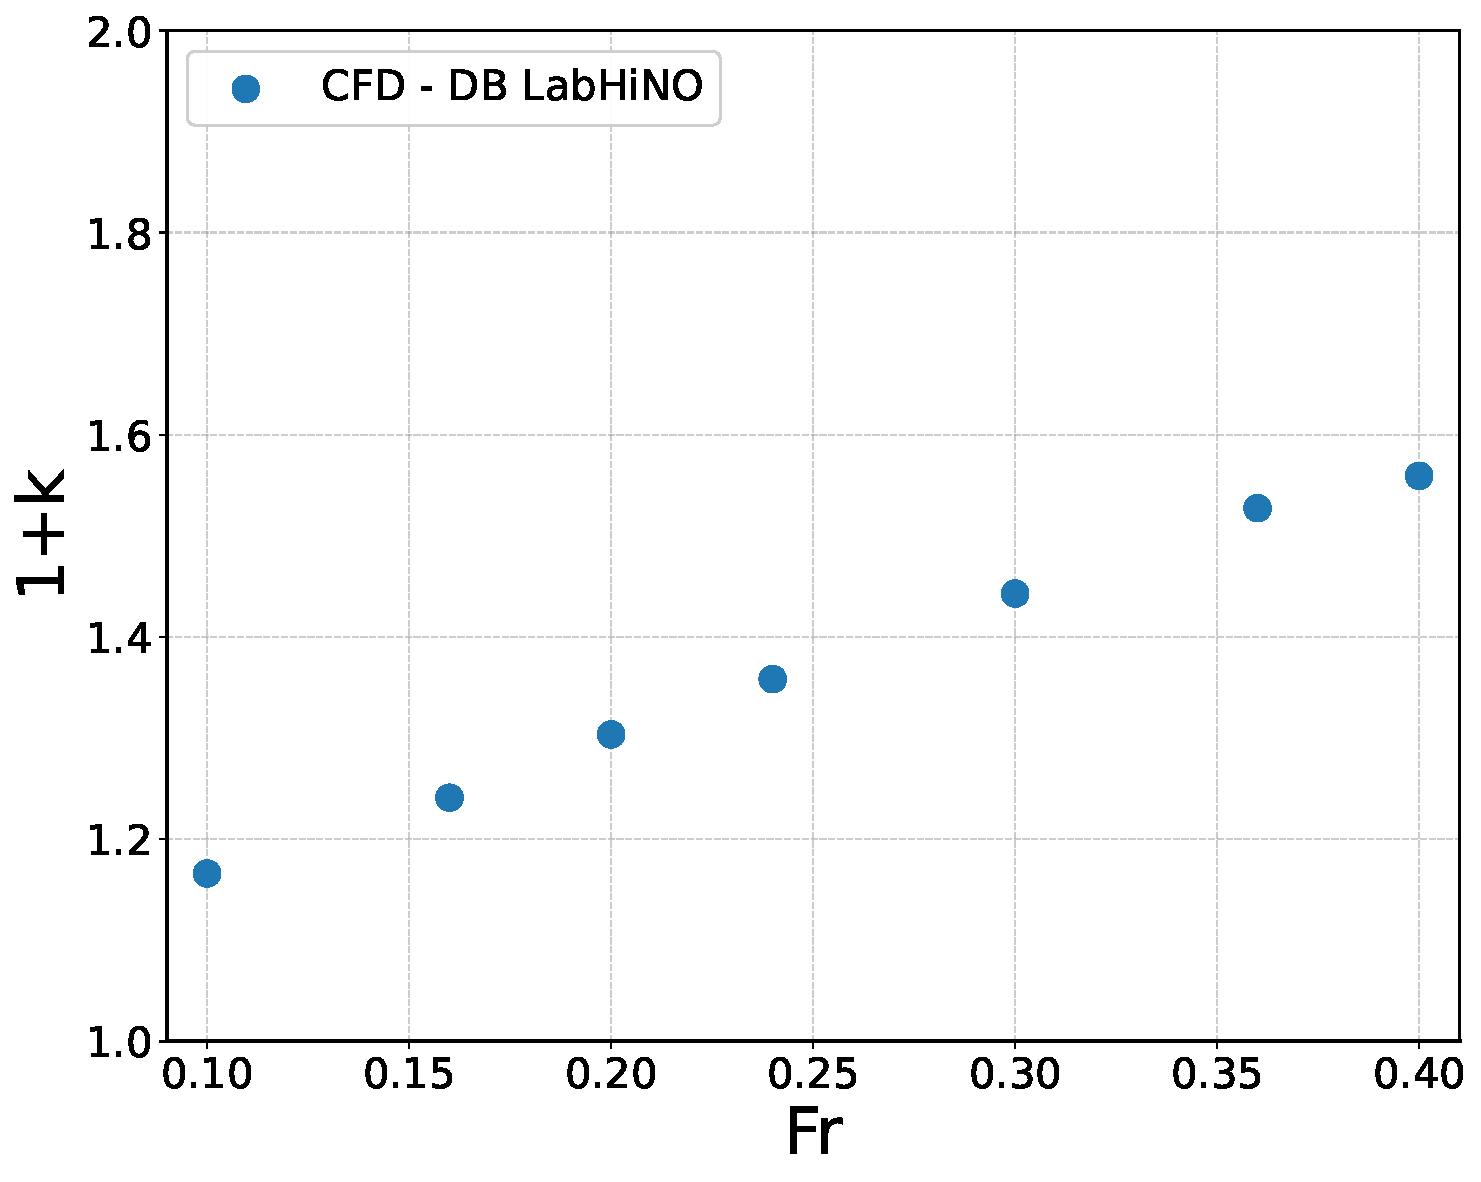
\includegraphics[width=\textwidth]{images/tpa_CFD_DB_165.pdf}
        \caption{Calado 1 (T1: 0.165 m)}
        \label{fig:k_165}
    \end{subfigure}
    \hfill
    \begin{subfigure}[b]{0.48\textwidth}
        \centering
        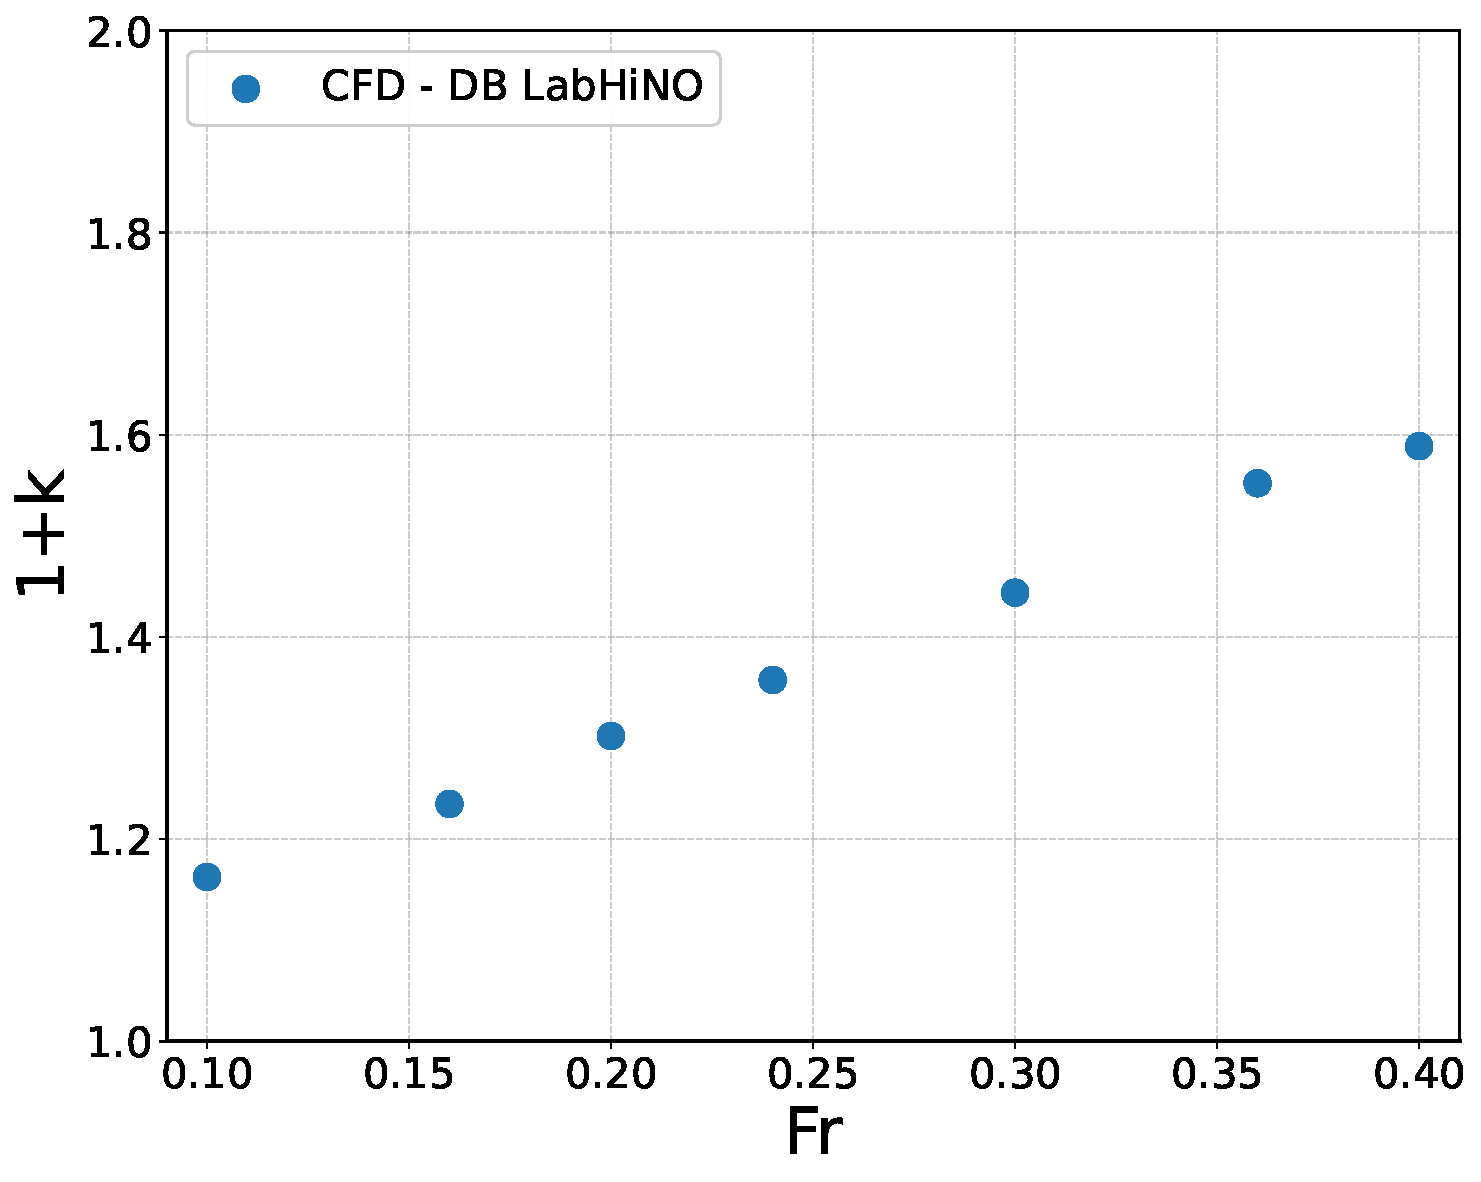
\includegraphics[width=\textwidth]{images/tpa_CFD_DB_180.pdf}
        \caption{Calado 2 (T2: 0.180 m)}
        \label{fig:k_180}
    \end{subfigure}
    
    \vspace{10pt} % Espacio entre filas
    
    % Segunda fila: Calado 3 centrado
    \begin{subfigure}[b]{0.48\textwidth}
        \centering
        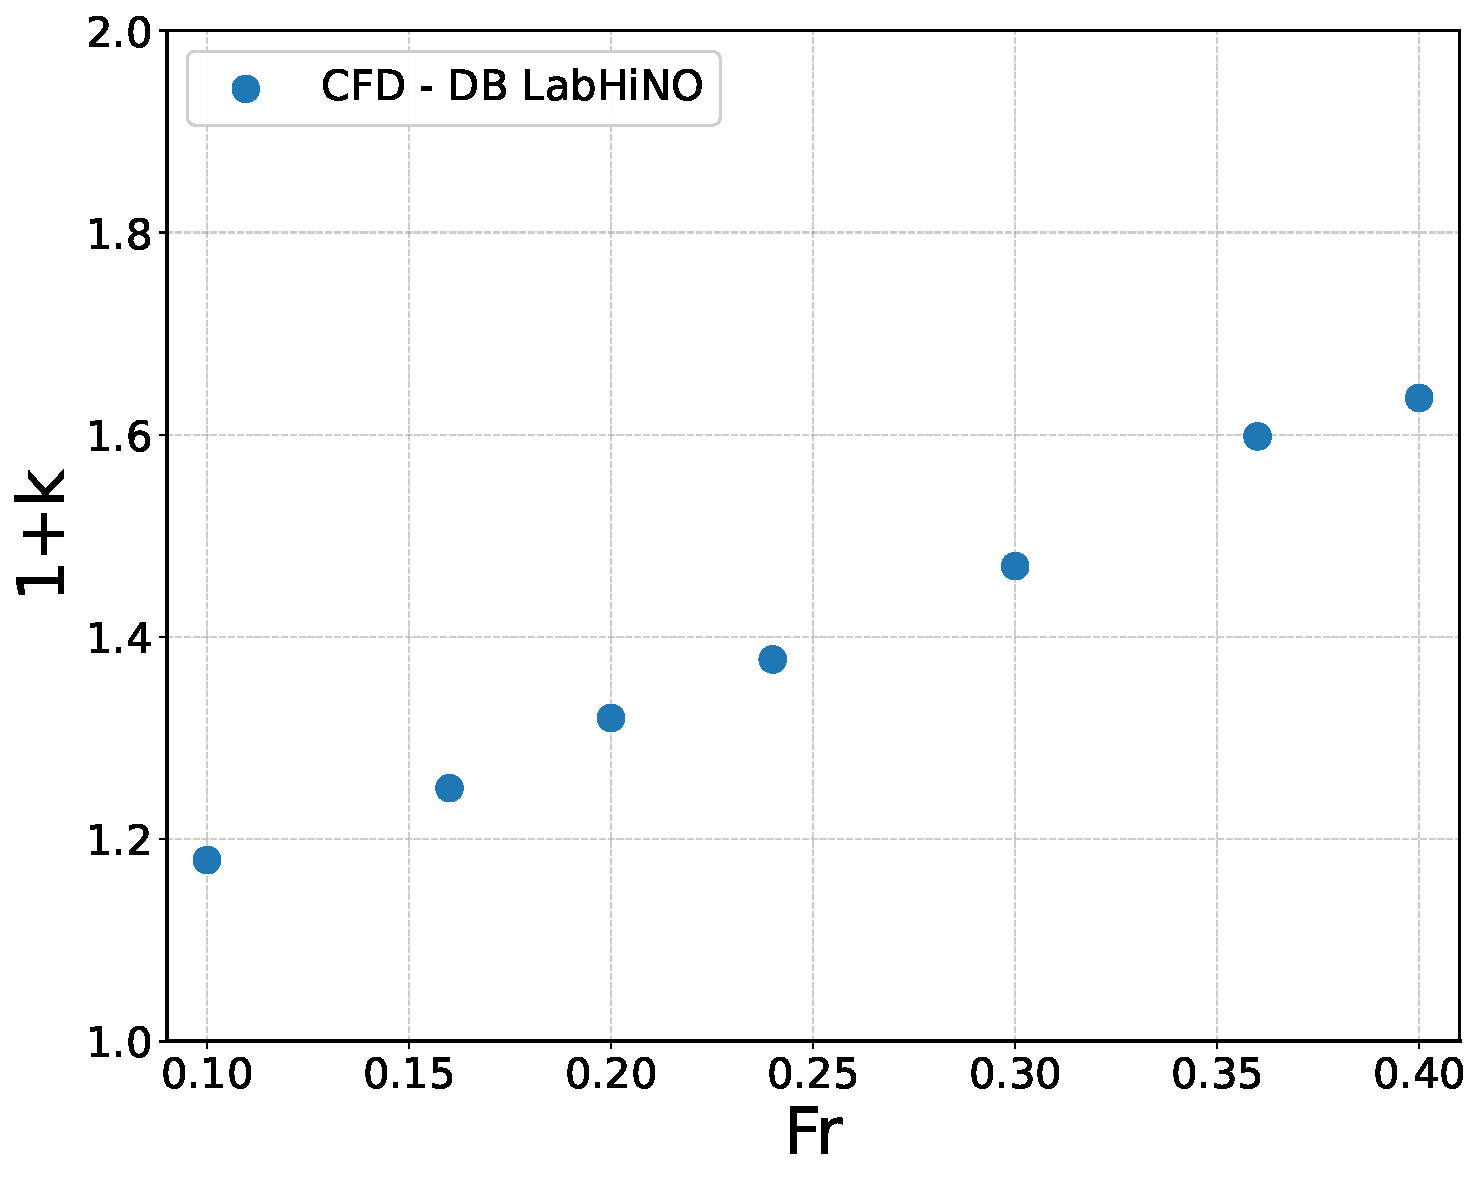
\includegraphics[width=\textwidth]{images/tpa_CFD_DB_195.pdf}
        \caption{Calado 3 (T3: 0.195 m)}
        \label{fig:k_195}
    \end{subfigure}

    \caption{Factor de forma calculado mediante el método de doble cuerpo para el \textit{P1} en los tres calados analizados, en función de Froude.}
    \label{fig:tpa_DB_k_evolucion}
\end{figure}

\subsubsection{Validación con modelo de referencia KCS}

Dada la variabilidad observada en el \textit{P1}, resulta necesario descartar 
que se trate de un error sistemático en la configuración del solver o del 
modelo de turbulencia. Para ello, se replicó exactamente la misma metodología 
sobre el modelo de referencia KCS (escala 1:79). La verificación numérica 
correspondiente se resume en la Tabla~\ref{tab:CFD_KCS}.

\begin{table}[htbp]
\centering
\caption{Verificación numérica para el modelo KCS a escala 1:79.}
\label{tab:CFD_KCS}
\small
\begin{tabular}{ccccc}
\toprule
\textbf{Fr} & \textbf{Re} & \boldmath{$y^+$} & \textbf{1+k} & \textbf{GCI [\%]} \\
\midrule
0.020 & $3.19\times10^{5}$ & 0.32 & 1.015 & 0.12 \\
0.040 & $6.37\times10^{5}$ & 0.91 & 1.022 & 0.06 \\
0.060 & $9.56\times10^{5}$ & 1.70 & 1.039 & 0.04 \\
0.080 & $1.28\times10^{6}$ & 2.64 & 1.101 & 0.01 \\
0.100 & $1.59\times10^{6}$ & 3.71 & 1.141 & 0.09 \\
0.120 & $1.91\times10^{6}$ & 4.90 & 1.218 & 0.07 \\
0.140 & $2.23\times10^{6}$ & 6.21 & 1.308 & 0.00 \\
0.160 & $2.55\times10^{6}$ & 7.61 & 1.314 & 0.01 \\
0.180 & $2.87\times10^{6}$ & 9.12 & 1.289 & 0.01 \\
0.200 & $3.19\times10^{6}$ & 10.71 & 1.254 & 0.04 \\
0.220 & $3.51\times10^{6}$ & 12.39 & 1.214 & 0.08 \\
0.240 & $3.82\times10^{6}$ & 14.16 & 1.182 & 0.11 \\
0.260 & $4.14\times10^{6}$ & 16.00 & 1.154 & 0.13 \\
0.280 & $4.46\times10^{6}$ & 17.92 & 1.131 & 0.20 \\
0.300 & $4.78\times10^{6}$ & 19.92 & 1.118 & 0.09 \\
0.320 & $5.10\times10^{6}$ & 21.98 & 1.118 & 0.43 \\
0.340 & $5.42\times10^{6}$ & 24.12 & 1.117 & 0.35 \\
0.360 & $5.74\times10^{6}$ & 26.32 & 1.114 & 1.06 \\
0.380 & $6.06\times10^{6}$ & 28.59 & 1.118 & 1.86 \\
0.400 & $6.37\times10^{6}$ & 30.93 & 1.117 & 1.09 \\
\bottomrule
\end{tabular}
\end{table}

A diferencia del \textit{P1}, el $y^+$ del KCS abarca desde la subcapa viscosa 
($y^+ \approx 0{.}3$) hasta el borde superior de la capa logarítmica 
($y^+ \approx 31$), atravesando la región \textit{buffer}. Pese a ello, la 
curva de $(1+k)$ resulta suave y sin cambios de pendiente, y el GCI se 
mantiene por debajo del $2\%$ en todo el rango. Esta robustez frente al 
tratamiento de pared se explica por la reducida contribución de la presión 
viscosa en este casco esbelto: al ser $C_{PV}$ una fracción pequeña de la 
resistencia viscosa total, el factor de forma queda dominado por $C_F$ y es 
poco sensible a la resolución de pared, en contraste con el \textit{P1}, donde 
$C_{PV}$ es comparable a $C_F$ (Sección~\ref{sec:descomposicion_de_la_res_viscosa}).

La Figura~\ref{fig:kcs_DB_prohaska} compara los resultados obtenidos con los 
reportados por \citet{TERZIEV2021147}. La concordancia es excelente, 
reproduciendo incluso la joroba característica en el rango de transición 
($Re \approx 10^6 - 3\times10^6$). Las líneas punteadas verticales indican 
los límites del rango de Froude recomendado por la ITTC para la aplicación 
del método de Prohaska ($Fr = 0.10$ y $Fr = 0.20$), correspondientes al 
modelo KCS a escala 1:79 ensayado en el LabHiNO, mientras que la línea 
horizontal continua representa el valor de $(1+k)$ adoptado a partir del 
ensayo experimental (EFD Prohaska, LabHiNO). Se observa que el valor 
experimental se ubica por debajo de los resultados CFD DB en ese rango, 
lo cual es consistente con la curvatura cóncava observada en el diagrama 
de Prohaska para las simulaciones numéricas, discutida en la 
Sección~\ref{sec:det_num_fac_form}.

\begin{figure}[htpb]
    \centering
    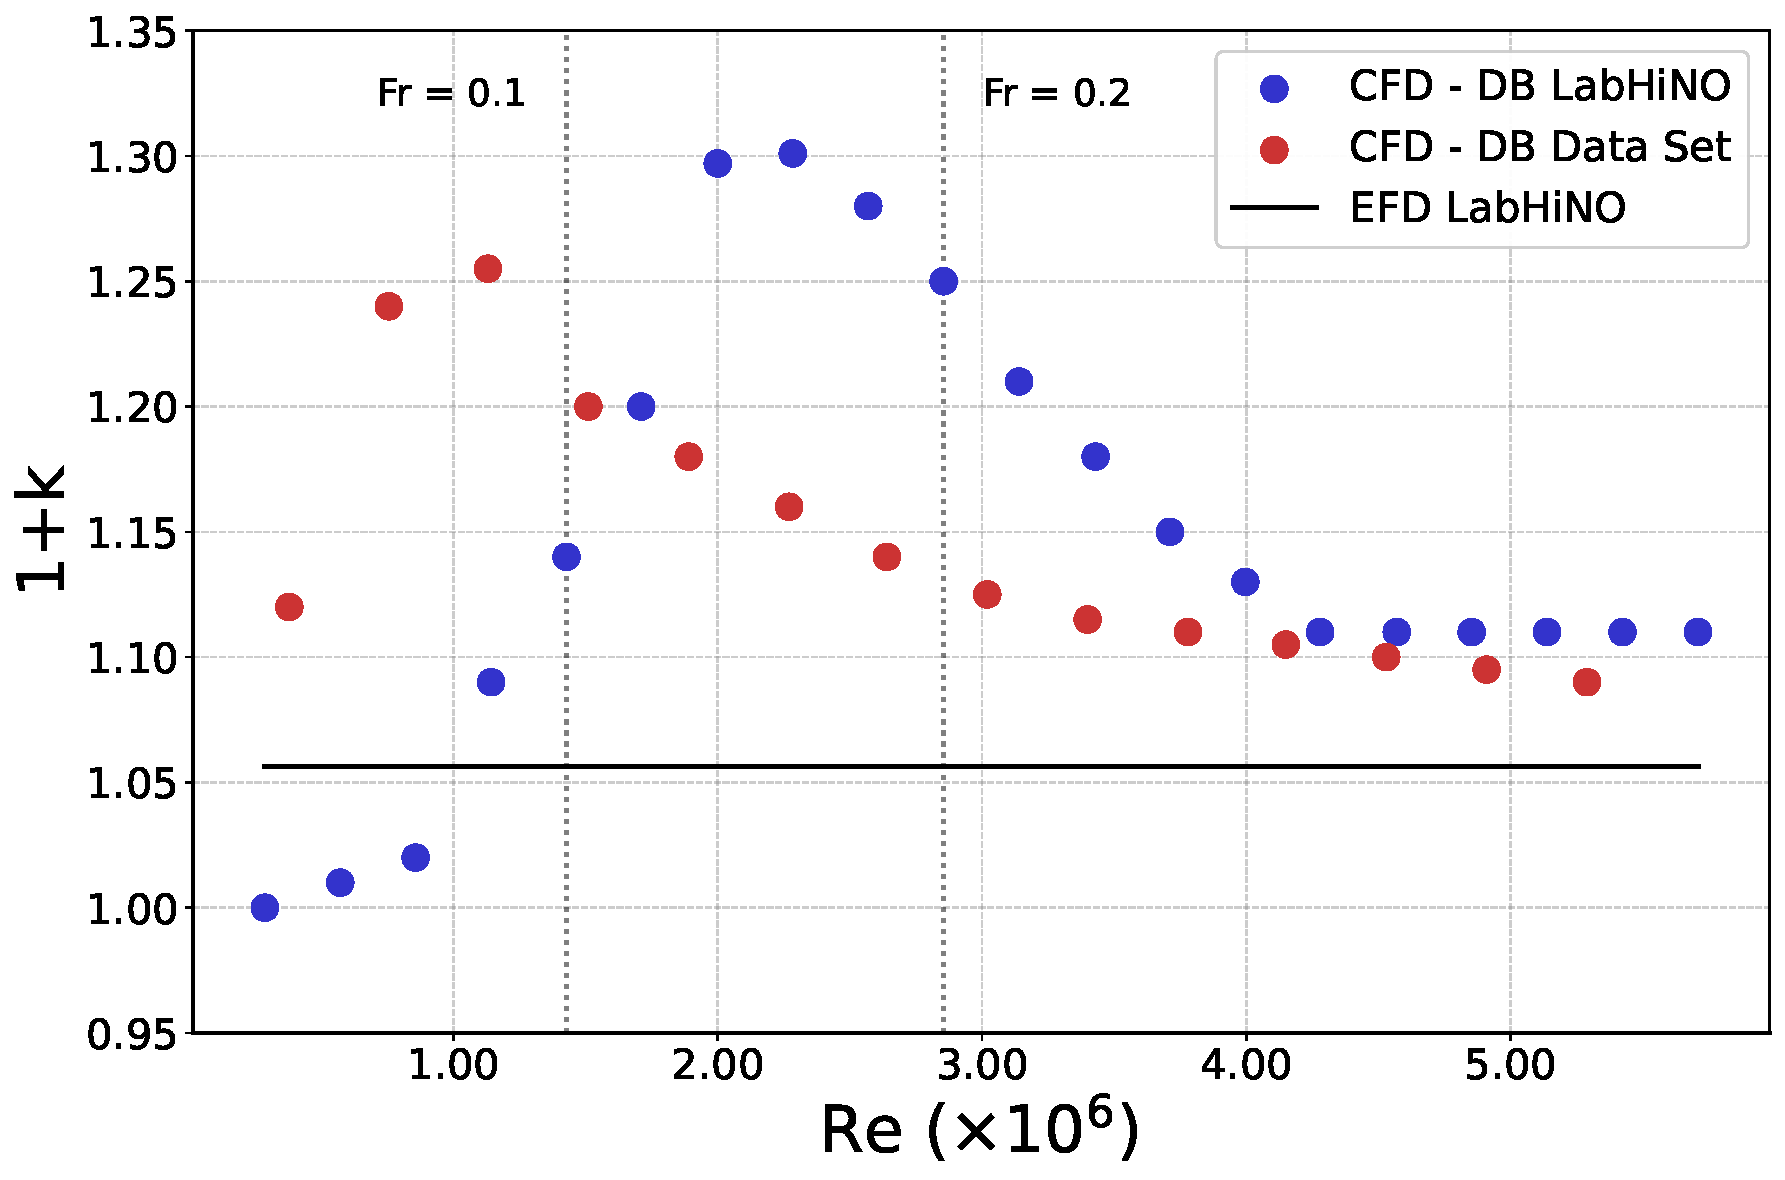
\includegraphics[width=.6\columnwidth]
        {images/kcs_DB_prohaska.pdf}
    \caption{Comparación de $1+k$ numérico vs $Re$ para el KCS 1:79 (escala LabHiNO) y 1:75 \citep{TERZIEV2021147}.}
    \label{fig:kcs_DB_prohaska}
\end{figure}

Finalmente, la Figura~\ref{fig:completo_kcs_lit} confirma que los resultados 
siguen la tendencia asintótica global validada por múltiples laboratorios 
internacionales \citep{TerzievDataSet}.

\begin{figure}[htpb]
    \centering
    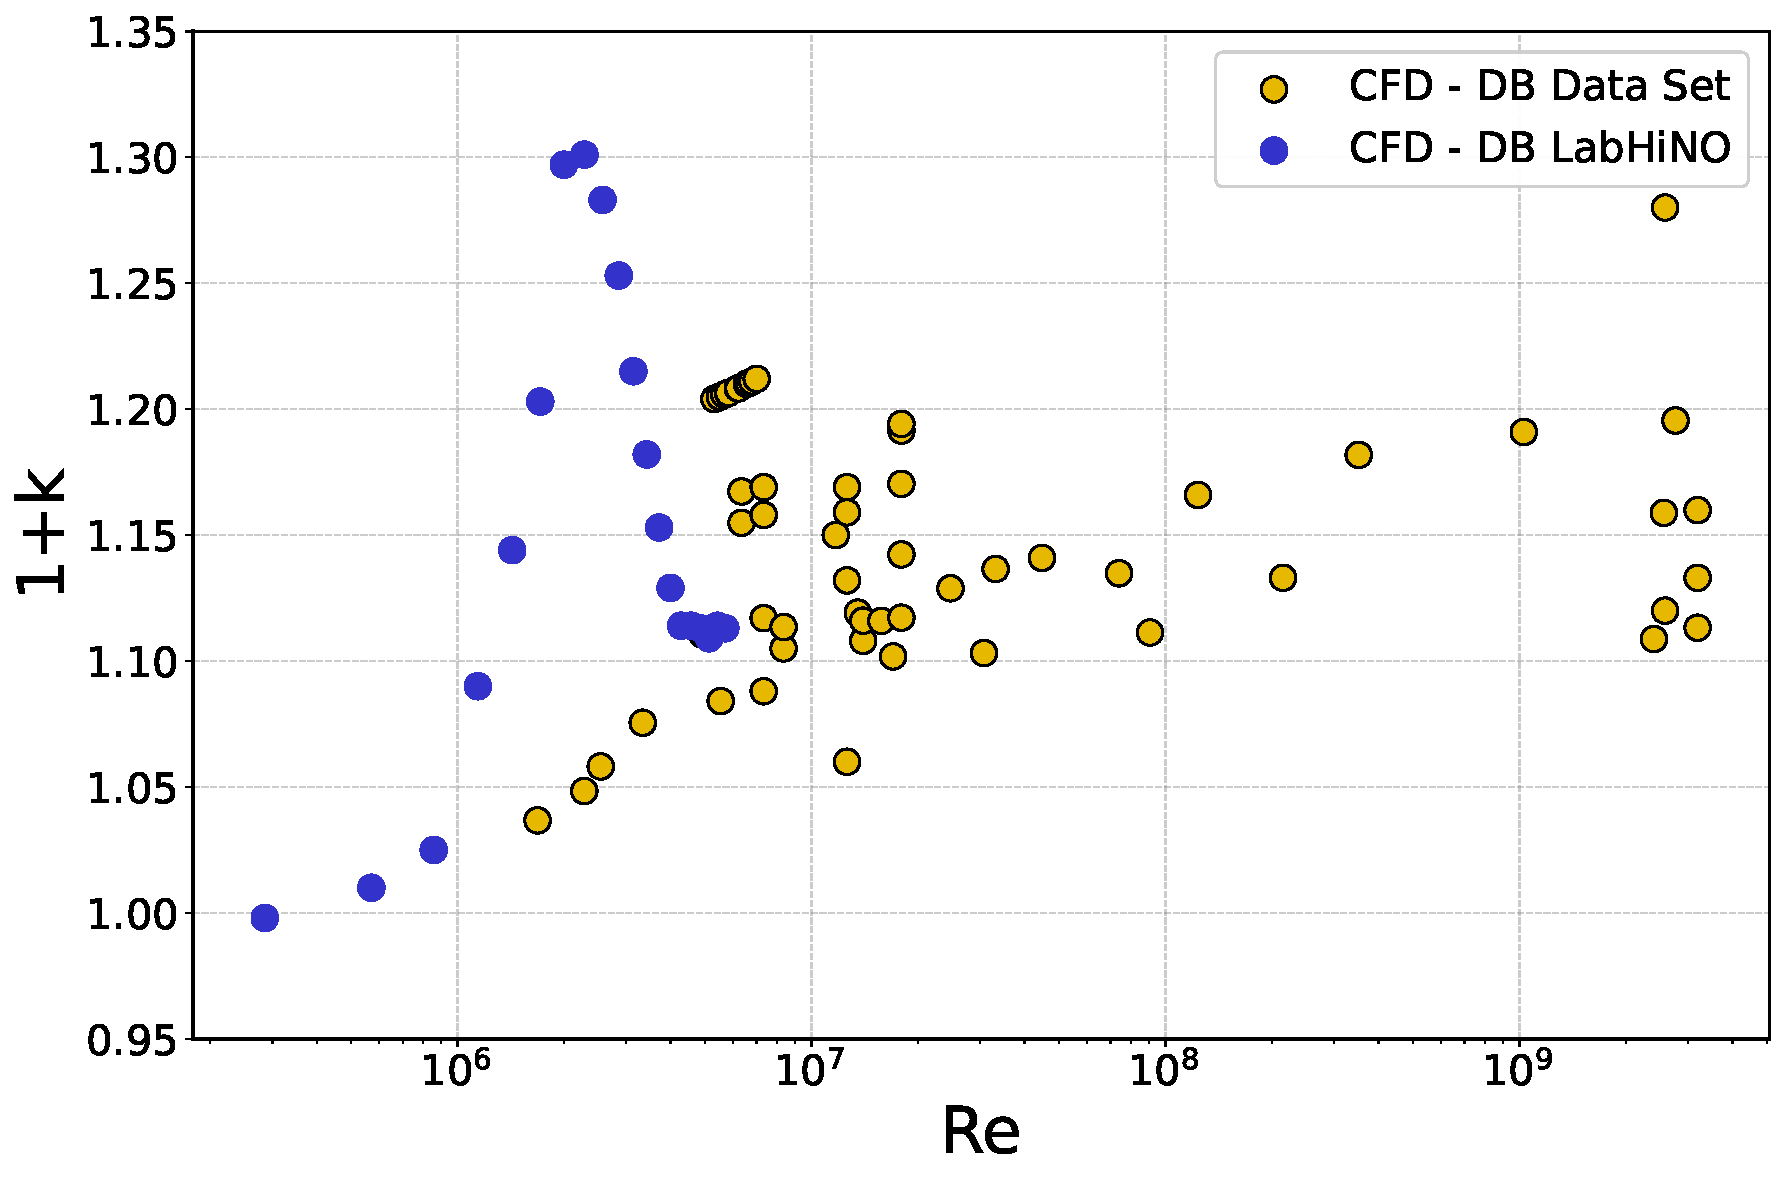
\includegraphics[width=.6\columnwidth]{images/cfd_kcs_lit.pdf}
    \caption{Factor de forma $(1+k)$ del KCS propio (CFD DB) frente a la base de datos \citep{TerzievDataSet}.}
    \label{fig:completo_kcs_lit}
\end{figure}

Esta validación cruzada permite afirmar que:
\begin{enumerate}
    \item La metodología numérica es correcta y precisa.
    \item La falta de estabilidad asintótica observada en el \textit{P1} no 
    es un error numérico ni un artefacto de la configuración del solver o del 
    modelo de turbulencia, sino una característica propia del casco analizado, 
    cuyo origen físico se analiza en profundidad en las secciones siguientes.
\end{enumerate}

\subsection{Comparación EFD CFD de resistencia y de factor de forma}

En esta sección se comparan los resultados experimentales y computacionales 
del \textit{P1} presentados en las secciones anteriores con el fin de 
sintetizar las diferencias encontradas. Esta comparación resulta central para 
el resto del análisis: dado que las simulaciones de doble cuerpo no admiten 
una validación experimental directa, al no existir un ensayo físico equivalente 
sin superficie libre, la confiabilidad del enfoque numérico completo descansa 
en la concordancia que aquí se establece entre el modelo bifásico con 
superficie libre y los ensayos de canal. Esta validación respalda, por 
extensión, la configuración numérica empleada (dominio, malla, modelo de 
turbulencia y condiciones de contorno) utilizada en las simulaciones de 
doble cuerpo presentadas en secciones posteriores.

\paragraph{Resistencia} Las Figuras~\ref{fig:resis_tpa_efd_cfd_165}
a~\ref{fig:resis_tpa_efd_cfd_195} comparan la resistencia experimental y
computacional del \textit{P1} para los tres calados. Para cuantificar
formalmente esta concordancia más allá de la inspección visual, se aplicó el
procedimiento de validación de la ITTC \citep{ITTC_uncertainty_CFD},
definiendo el error de comparación entre el valor experimental $D$ y el
numérico $S$ como $E\%D = (D-S)/D\times100$, y la incertidumbre de validación
como $U_{val}=\sqrt{U_D^2+U_{num}^2}$, con $U_D$ la incertidumbre experimental
(Tabla~\ref{tab:uncert_tpa}) y $U_{num}$ la numérica derivada del GCI. La
solución se considera validada, dentro de la incertidumbre disponible, cuando
$|E\%D|\le U_{val}$.

La validación formal se presenta para el Calado~2
(Tabla~\ref{tab:validacion_efd_cfd}), cuyos ensayos y simulaciones cubren el
rango operativo con una grilla de velocidades coincidente. El error de
comparación se mantiene dentro de la incertidumbre de medición hasta
$Fr \approx 0{.}26$, con un valor medio del orden del $1{.}5\%$ en ese
intervalo. A partir de $Fr \approx 0{.}29$ el modelo numérico subestima la
resistencia de manera creciente; esta desviación es atribuible a la
restricción de grados de libertad del modelo numérico —fijo en cabeceo y
hundimiento, frente al modelo libre del ensayo— y no a un error del modelo
físico, y ocurre además fuera del rango de operación del \textit{P1}. Los
puntos de $Fr < 0{.}18$ se excluyen del análisis por la baja relación
señal--ruido característica del régimen de baja resistencia.

\begin{table}[htbp]
\centering
\caption{Validación EFD--CFD de la resistencia total del \textit{P1}
(Calado~2, $T=0{.}180$~m) en el rango operativo. Error de comparación
$E\%D=(D-S)/D\times100$; incertidumbre de validación
$U_{val}=\sqrt{U_D^2+U_{num}^2}\approx U_D$, siendo $U_{num}<0{.}2\%$
despreciable frente a $U_D$ en este rango.}
\label{tab:validacion_efd_cfd}
\small
\begin{tabular}{ccccc}
\toprule
\textbf{Fr} & \boldmath{$E\%D$ [\%]} & \boldmath{$U_D$ [\%]} &
\boldmath{$U_{val}$ [\%]} & \textbf{¿Validado?} \\
\midrule
0.20 & $-2{.}4$ & 3.7 & 3.7 & Sí \\
0.22 & $-0{.}1$ & 3.1 & 3.1 & Sí \\
0.24 & $\phantom{-}1{.}3$ & 2.6 & 2.6 & Sí \\
0.26 & $\phantom{-}1{.}0$ & 2.0 & 2.0 & Sí \\
0.29 & $\phantom{-}4{.}1$ & 1.7 & 1.7 & No \\
0.32 & $\phantom{-}4{.}7$ & 1.4 & 1.4 & No \\
\bottomrule
\end{tabular}
\end{table}

El mismo análisis se aplicó a los calados restantes. Para el Calado~1
($T=0{.}165$~m), el error de comparación medio en el rango operativo es del
orden del $5\%$, mayor que en el Calado~2 y asociado a una mayor dispersión de
las corridas CFD en esa condición; aun así se mantiene dentro de márgenes
habituales para la predicción de resistencia por CFD. Para el Calado~3
($T=0{.}195$~m), los ensayos experimentales y las simulaciones se realizaron
sobre grillas de $Fr$ no coincidentes, por lo que la comparación se efectúa
interpolando la curva CFD a las velocidades ensayadas; sobre los puntos
comparables del rango operativo, la concordancia entre las curvas experimental
y computacional es del orden del $1$--$2\%$, consistente con la obtenida para
los demás calados.

En conjunto, la concordancia EFD--CFD en el rango operativo respalda la
confiabilidad del modelo numérico con superficie libre y, por extensión, de
las simulaciones de doble cuerpo, que carecen de contrapartida experimental
directa (Sección~\ref{sec:4.1.5_enfoque_doble_cuerpo}).

\begin{figure}[htpb]
     \centering
     \begin{subfigure}[b]{0.45\textwidth}
         \centering
         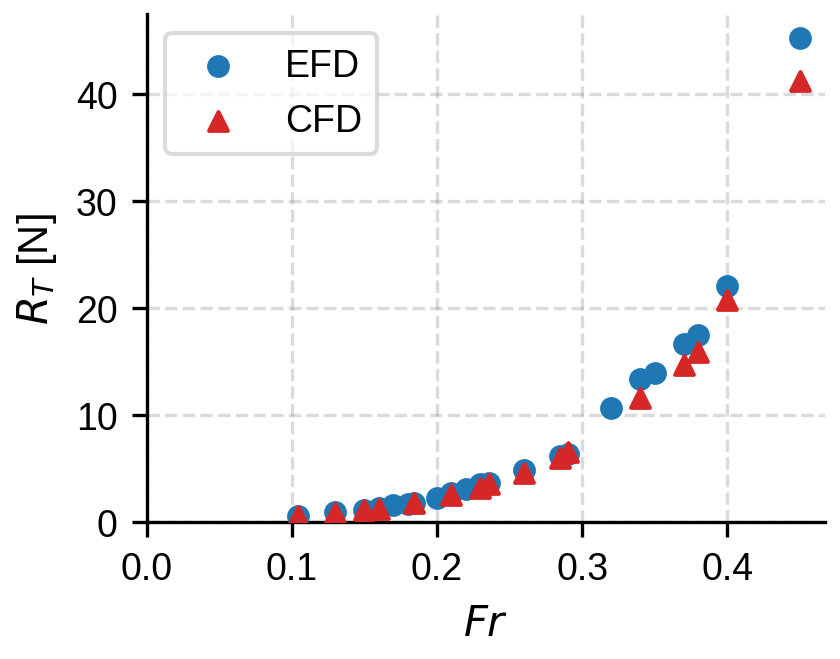
\includegraphics[width=\textwidth]{images/efd-cfd-165}
         \caption{Calado 1.}
         \label{fig:resis_tpa_efd_cfd_165}
     \end{subfigure}
     \hfill
     \begin{subfigure}[b]{0.45\textwidth}
         \centering
         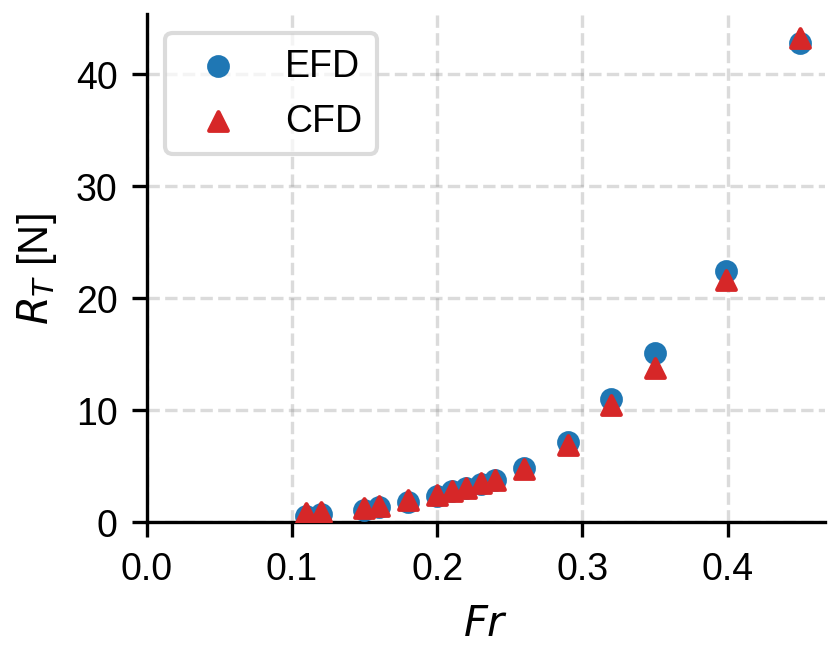
\includegraphics[width=\textwidth]{images/efd-cfd-180}
         \caption{Calado 2.}
         \label{fig:resis_tpa_efd_cfd_180}
     \end{subfigure}

     \vspace{0.5cm}

     \begin{subfigure}[b]{0.45\textwidth}
         \centering
         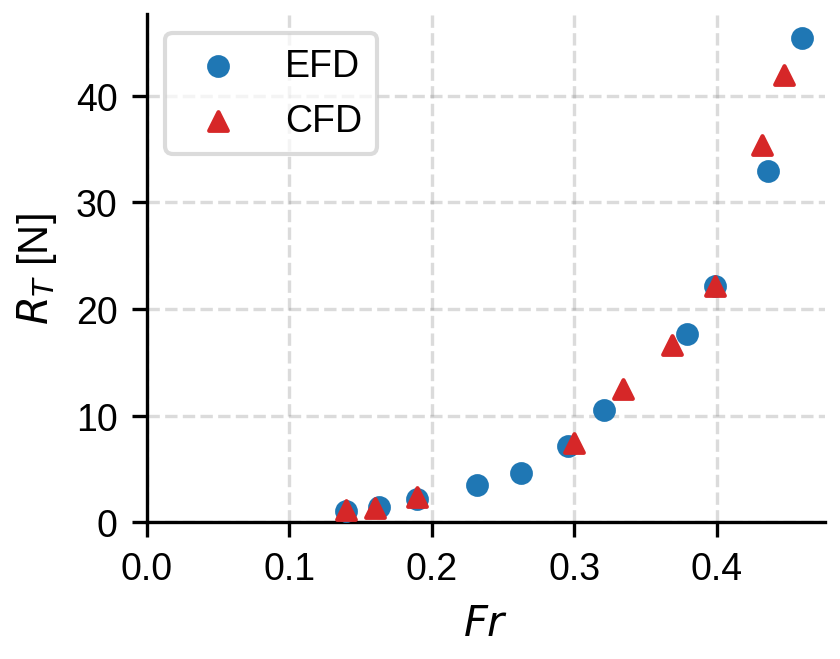
\includegraphics[width=\textwidth]{images/efd-cfd-195}
         \caption{Calado 3.}
         \label{fig:resis_tpa_efd_cfd_195}
     \end{subfigure}

     \caption{Resistencia al avance del \textit{P1} en función de $Fr$. 
     Comparación EFD--CFD para los tres calados.}
     \label{fig:comparativa_efd_cfd_calados}
\end{figure}

\paragraph{Factor de forma} Como fue mencionado en las secciones 
\ref{sec:det_exp_fac_form} y \ref{sec:det_num_fac_form}, tanto para el cálculo 
experimental como para el computacional, no es posible ajustar adecuadamente 
la recta esperada por el método de Prohaska a bajas velocidades. Las 
Figuras~\ref{fig:prohaska_tpa_efd_cfd_165} a \ref{fig:prohaska_tpa_efd_cfd_195} 
superponen los diagramas de Prohaska del \textit{P1} obtenidos mediante EFD 
(recta D2) y CFD (recta D1) para cada calado, junto con los puntos 
correspondientes a cada enfoque. Ambas rectas representan la extrapolación 
lineal sobre el rango $0.10 < Fr < 0.20$, cuya ordenada al origen determina 
el valor de $(1+k)$ adoptado en cada caso. Se observa que las rectas EFD y 
CFD se cruzan en un punto intermedio del rango analizado, lo que indica que 
la desviación respecto de la linealidad teórica tiene signo opuesto en ambos 
enfoques: mientras que los puntos experimentales tienden a curvarse de forma 
convexa, los puntos numéricos lo hacen de forma cóncava. Como se discutió en 
la Sección~\ref{sec:prohaska_antec}, esta desviación puede atribuirse a 
múltiples causas, entre ellas la laminarización parcial del flujo, la 
geometría de la proa bulbo, la separación de flujo en popa y el sesgo 
introducido por la línea de correlación ITTC-1957. En el caso particular de 
las simulaciones CFD, la curvatura cóncava observada es consistente con la 
incapacidad del modelo de turbulencia $k$-$\omega$ SST de reproducir 
correctamente la zona de transición a bajos $Re$.

\begin{figure}[htpb]
\centering
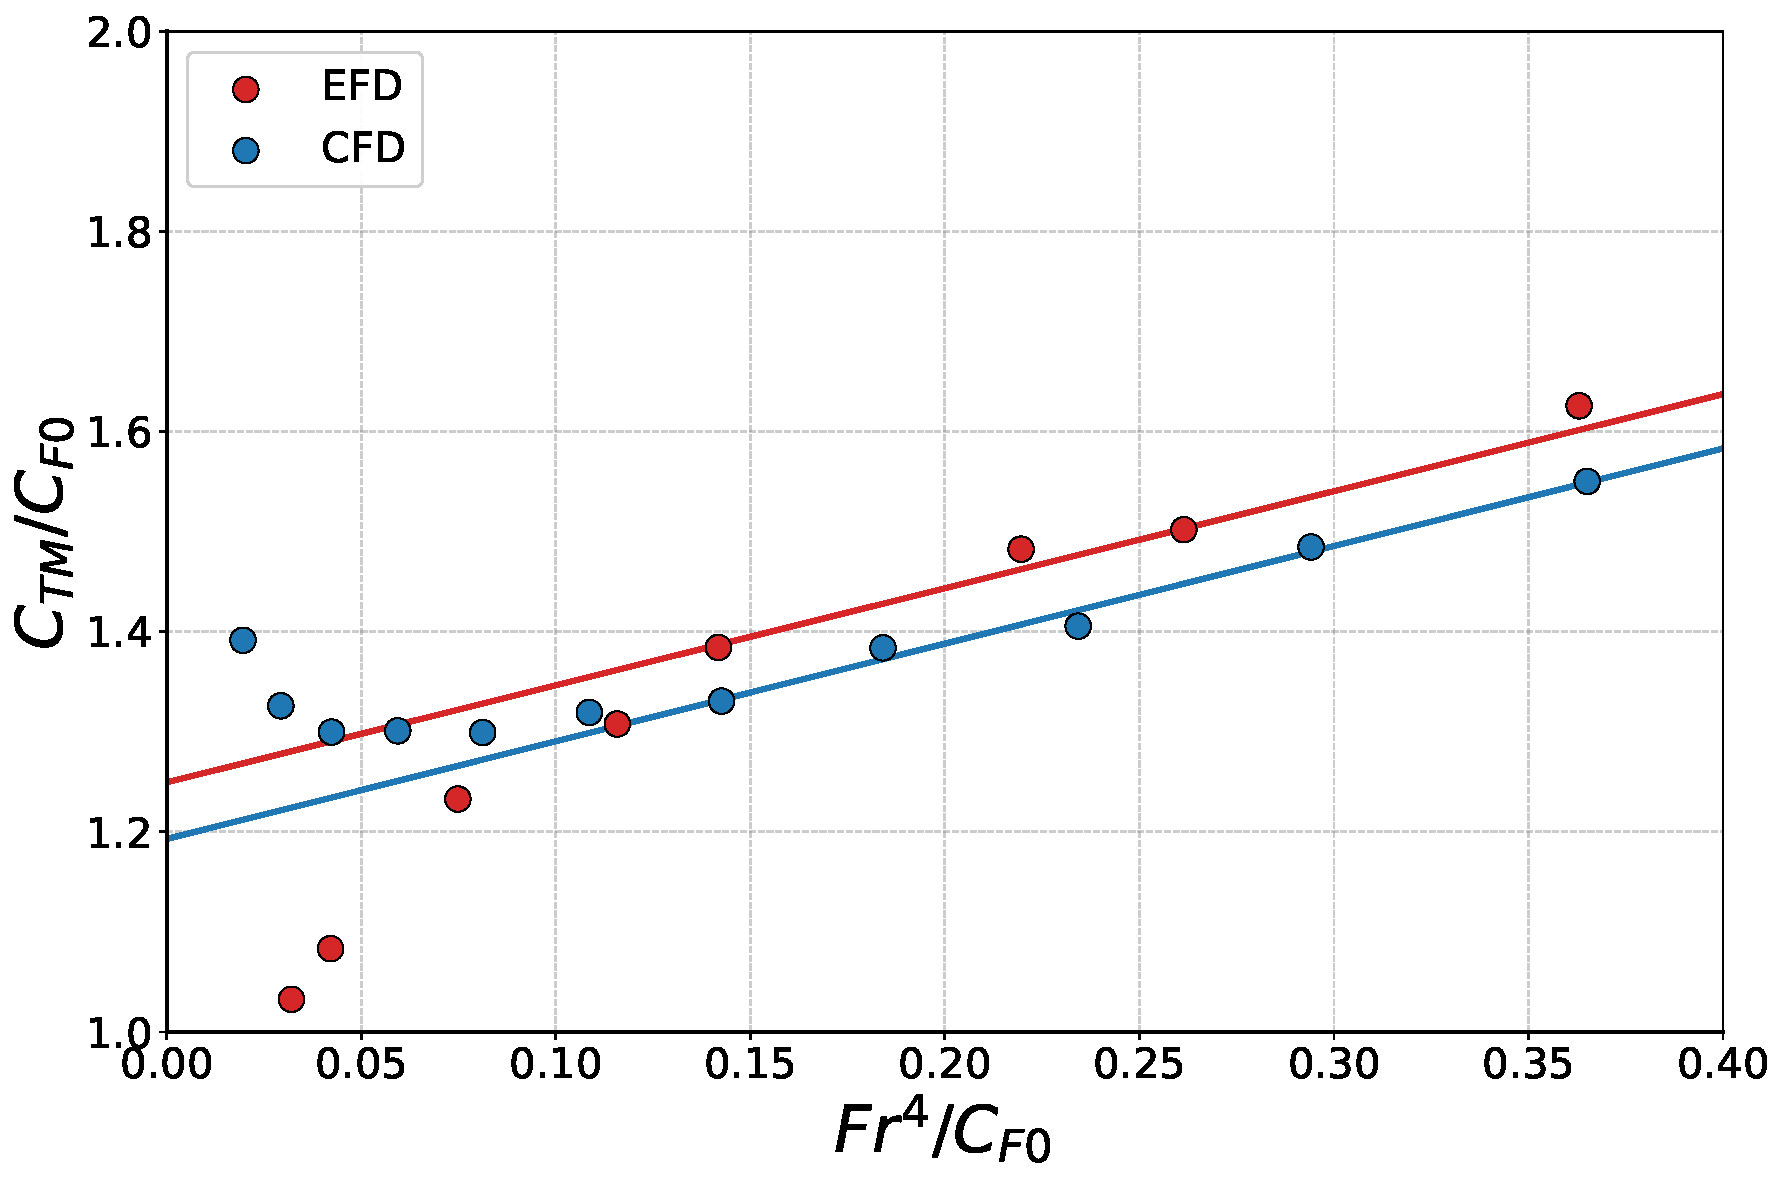
\includegraphics[width=0.6\textwidth]{images/prohaska-efd-cfd-165.pdf}
\caption{Diagrama de Prohaska del \textit{P1} comparando EFD y CFD. Calado 1.}
\label{fig:prohaska_tpa_efd_cfd_165}
\end{figure}

\begin{figure}[htpb]
\centering
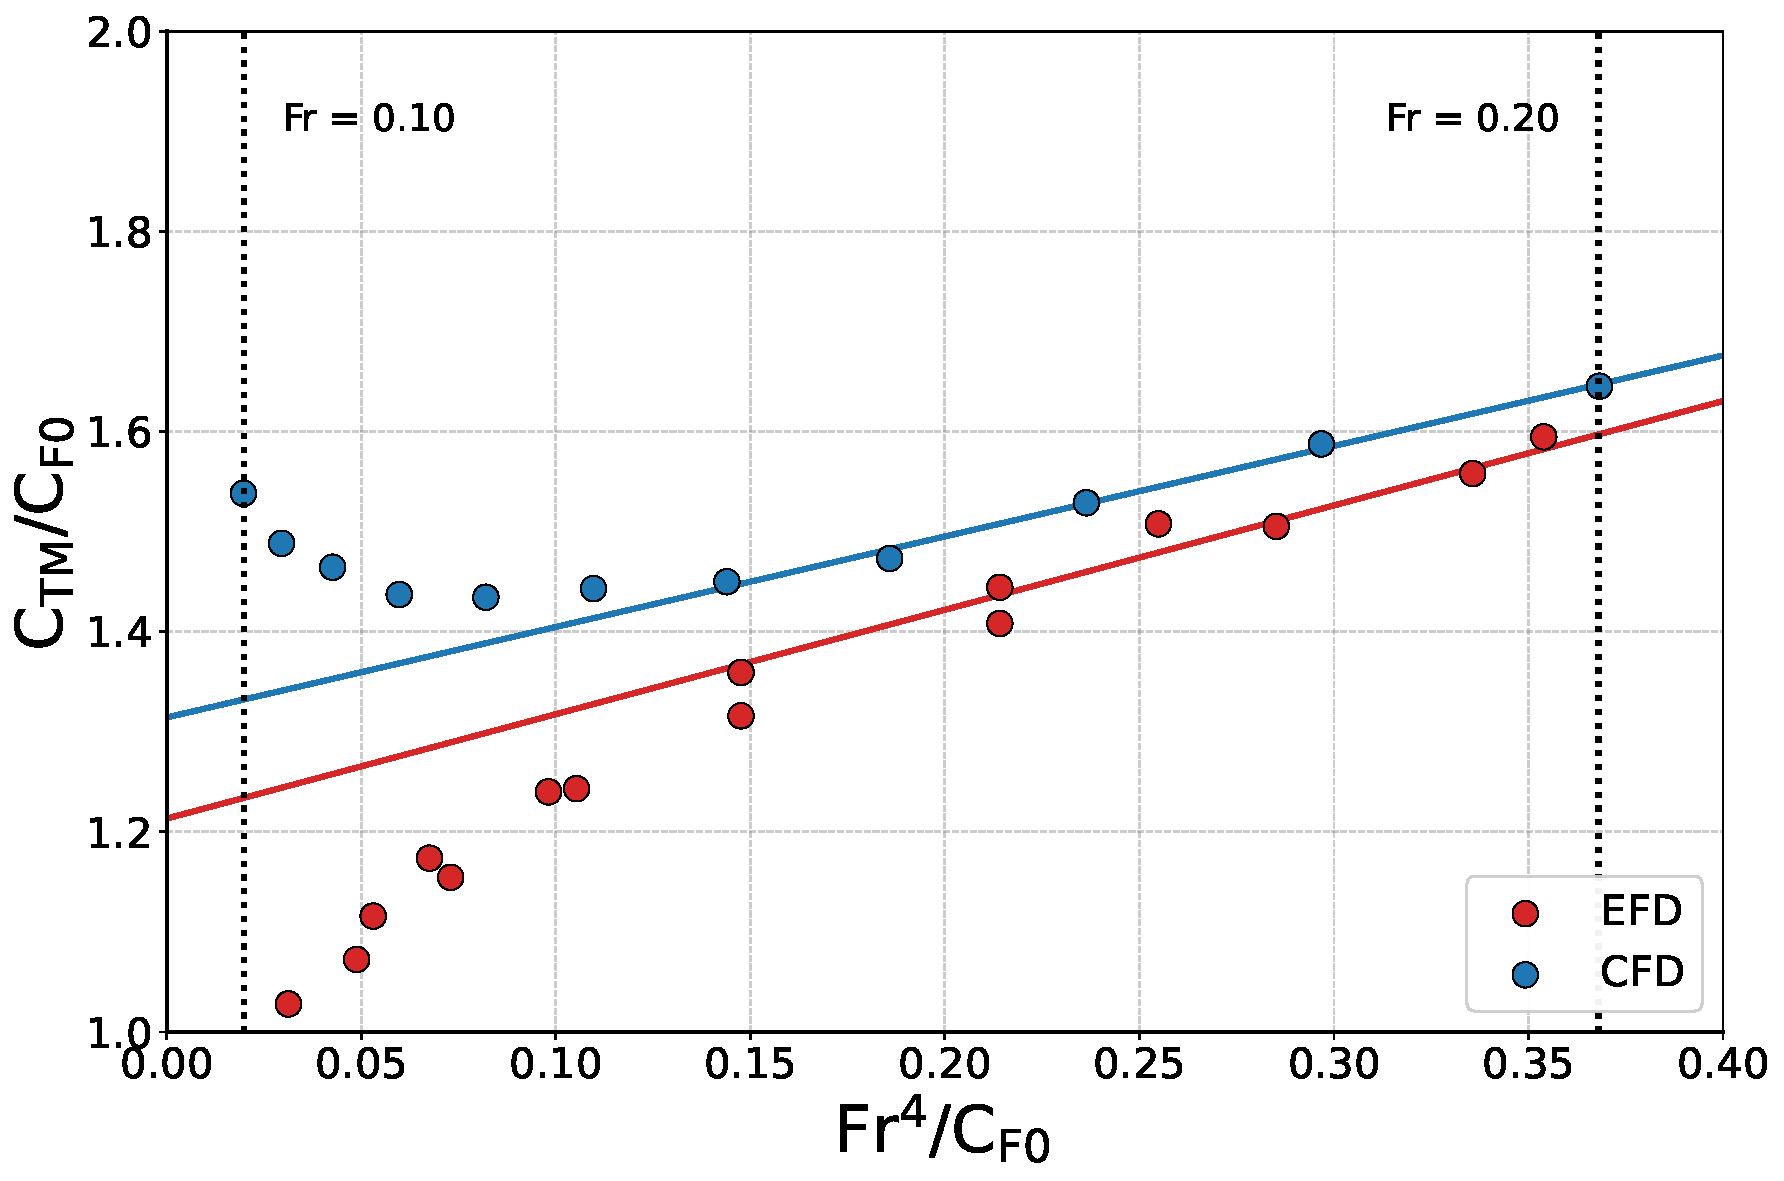
\includegraphics[width=0.6\textwidth]{images/prohaska-efd-cfd-180.pdf}
\caption{Diagrama de Prohaska del \textit{P1} comparando EFD y CFD. Calado 2.}
\label{fig:prohaska_tpa_efd_cfd_180}
\end{figure}

\begin{figure}[htpb]
\centering
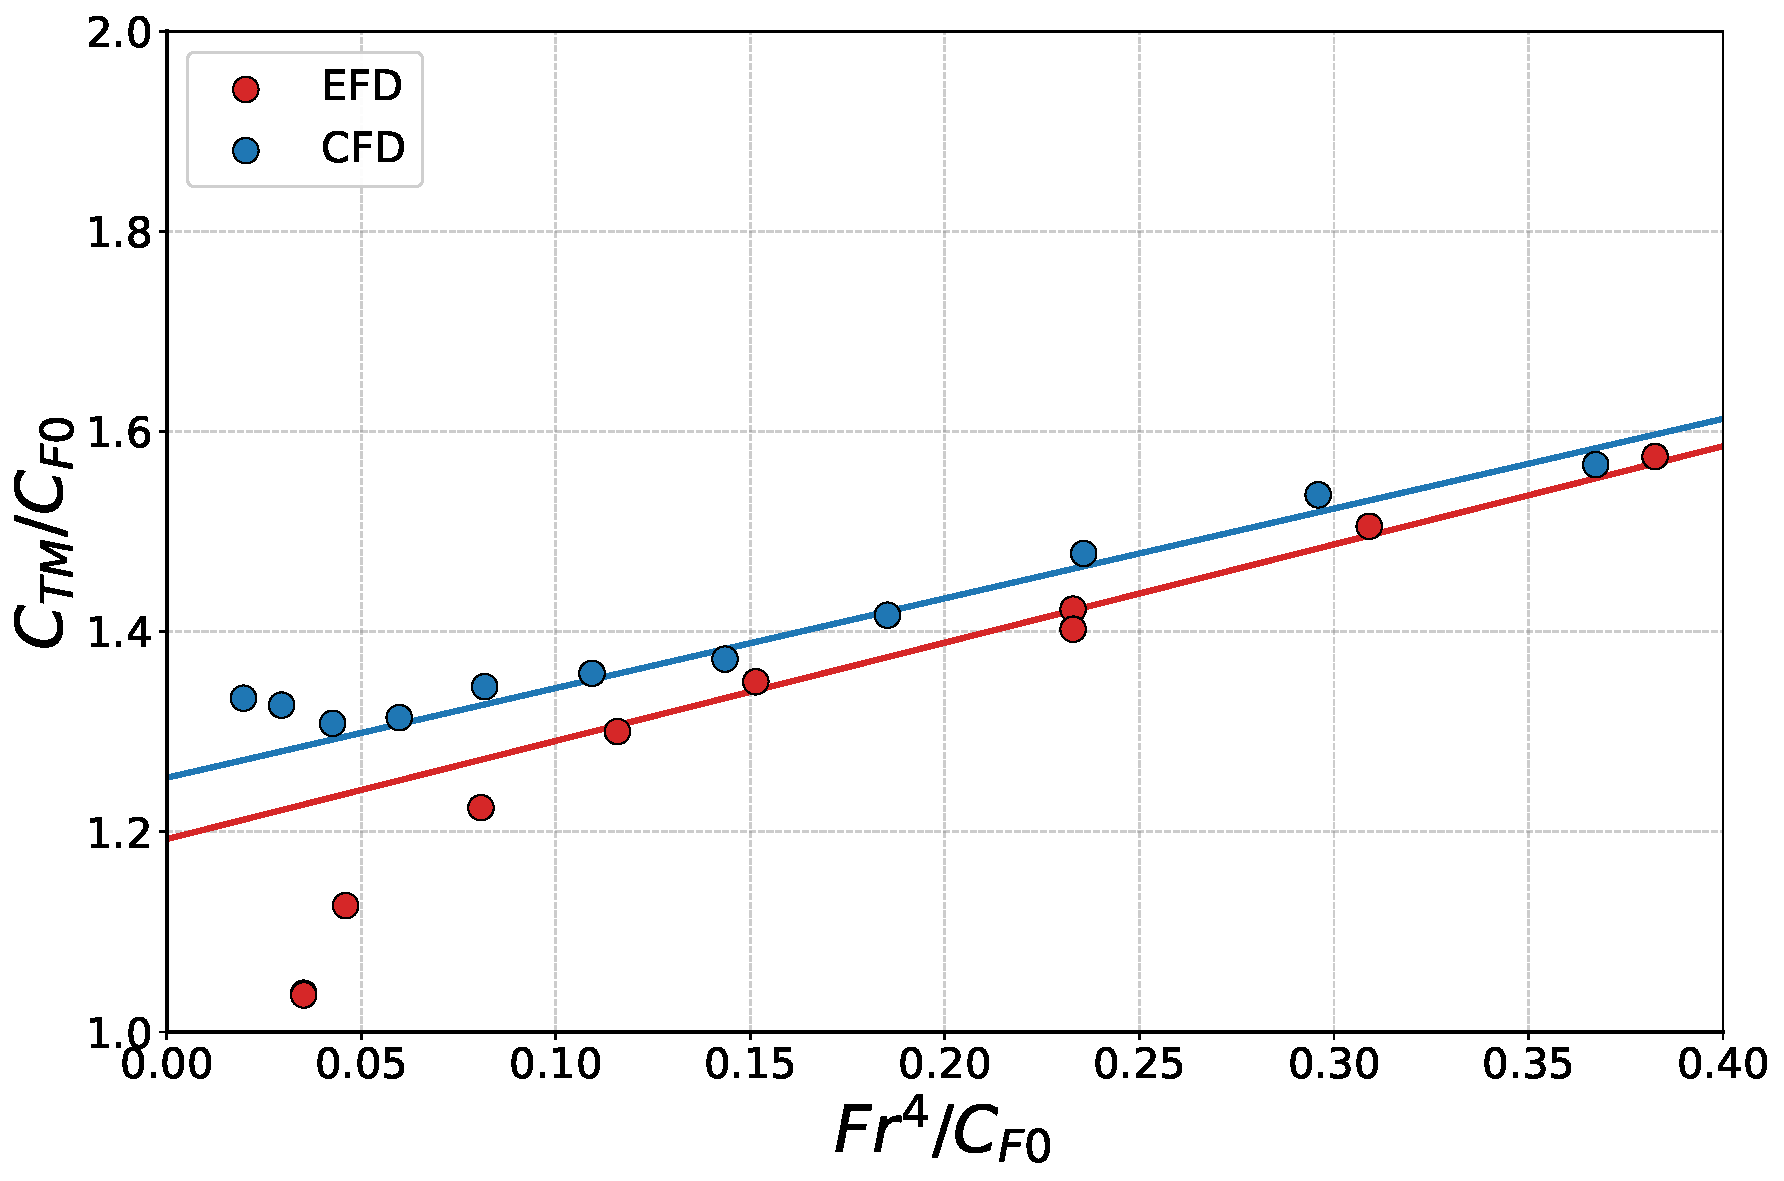
\includegraphics[width=0.6\textwidth]{images/prohaska-efd-cfd-195.pdf}
\caption{Diagrama de Prohaska del \textit{P1} comparando EFD y CFD. Calado 3.}
\label{fig:prohaska_tpa_efd_cfd_195}
\end{figure}

La Figura~\ref{fig:comparativa_form_factor_range} muestra, para cada calado, 
el valor de $(1+k)$ obtenido por Prohaska al variar el límite inferior del 
rango de Froude considerado en la regresión, tanto para EFD como para CFD. 
Se observa que, al restringir el rango a $0.13 < Fr < 0.18$ aproximadamente, 
ambos enfoques convergen a un valor prácticamente idéntico, eliminando la 
discrepancia inicial observada a bajas velocidades. Este resultado confirma 
que, dentro del rango adecuado de aplicación del método, tanto el ensayo 
experimental como la simulación numérica con superficie libre predicen el 
mismo factor de forma para el \textit{P1}.

\begin{figure}[htpb]
     \centering
     \begin{subfigure}[b]{0.48\textwidth}
         \centering
         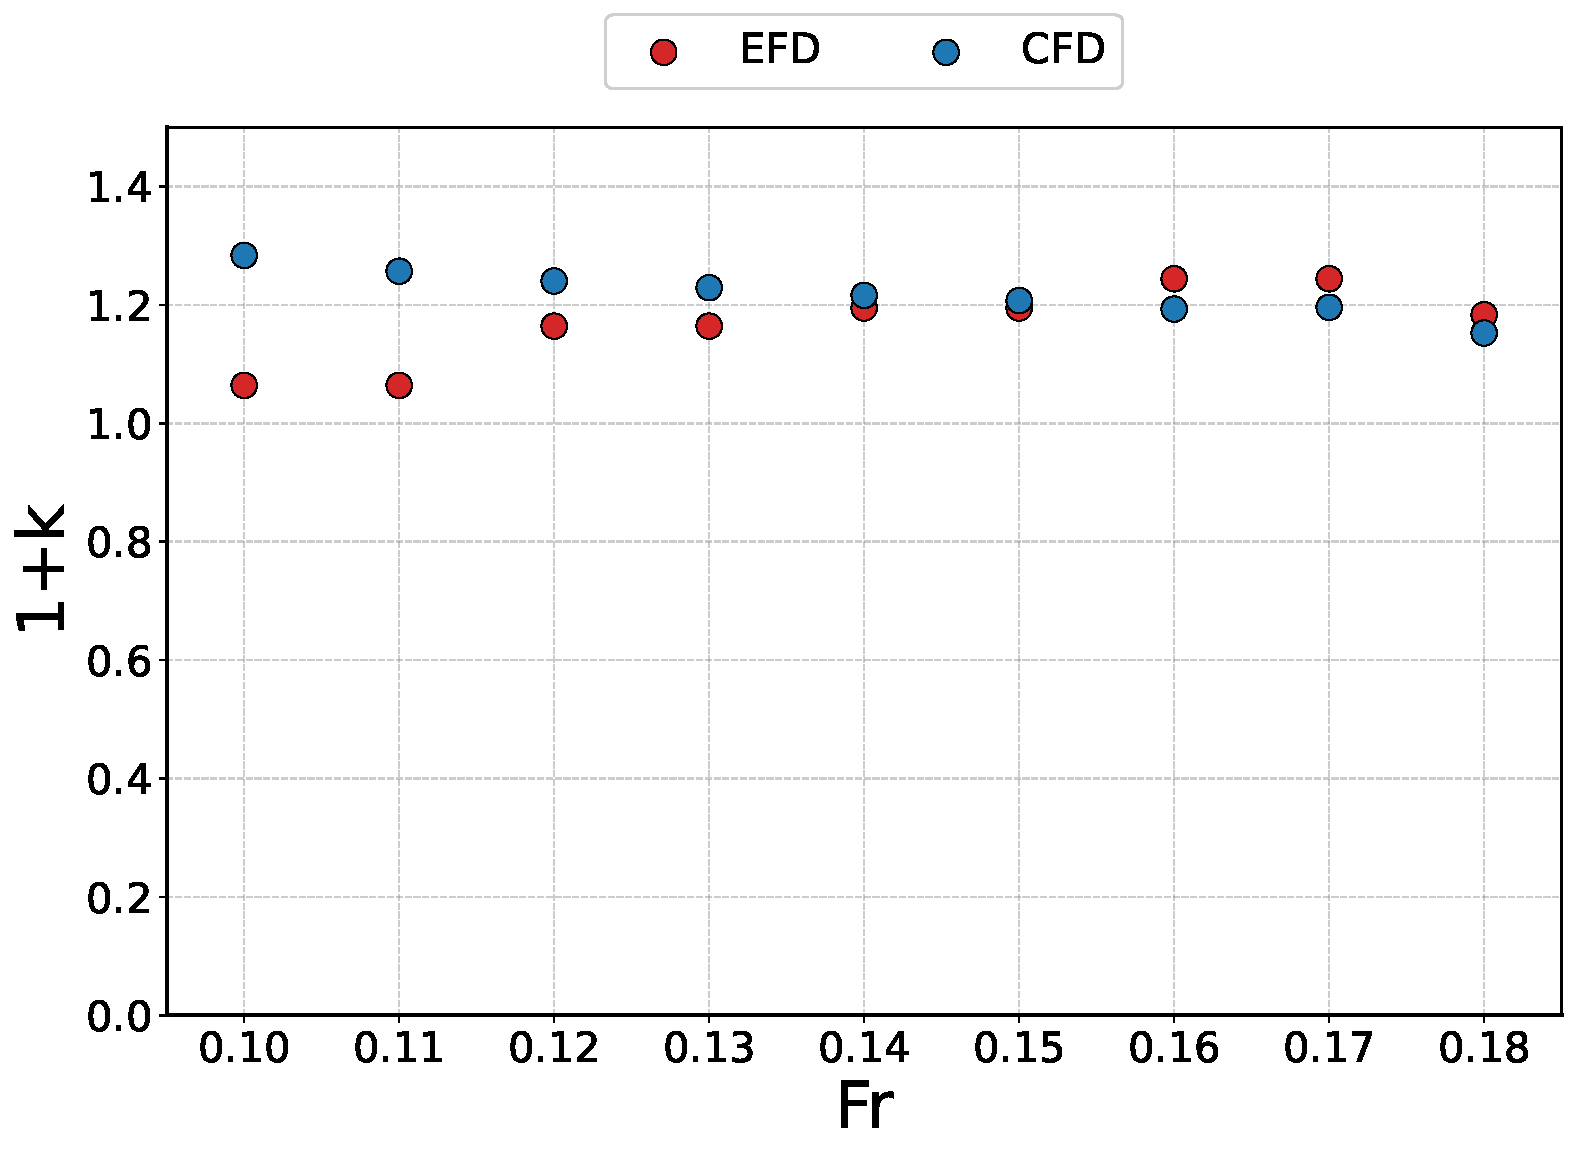
\includegraphics[width=\textwidth]{images/efd_cfd_form_factor_tpa_165_range}
         \caption{Calado 1.}
         \label{fig:efd_cfd_165_tpa_range}
     \end{subfigure}
     \hfill
     \begin{subfigure}[b]{0.48\textwidth}
         \centering
         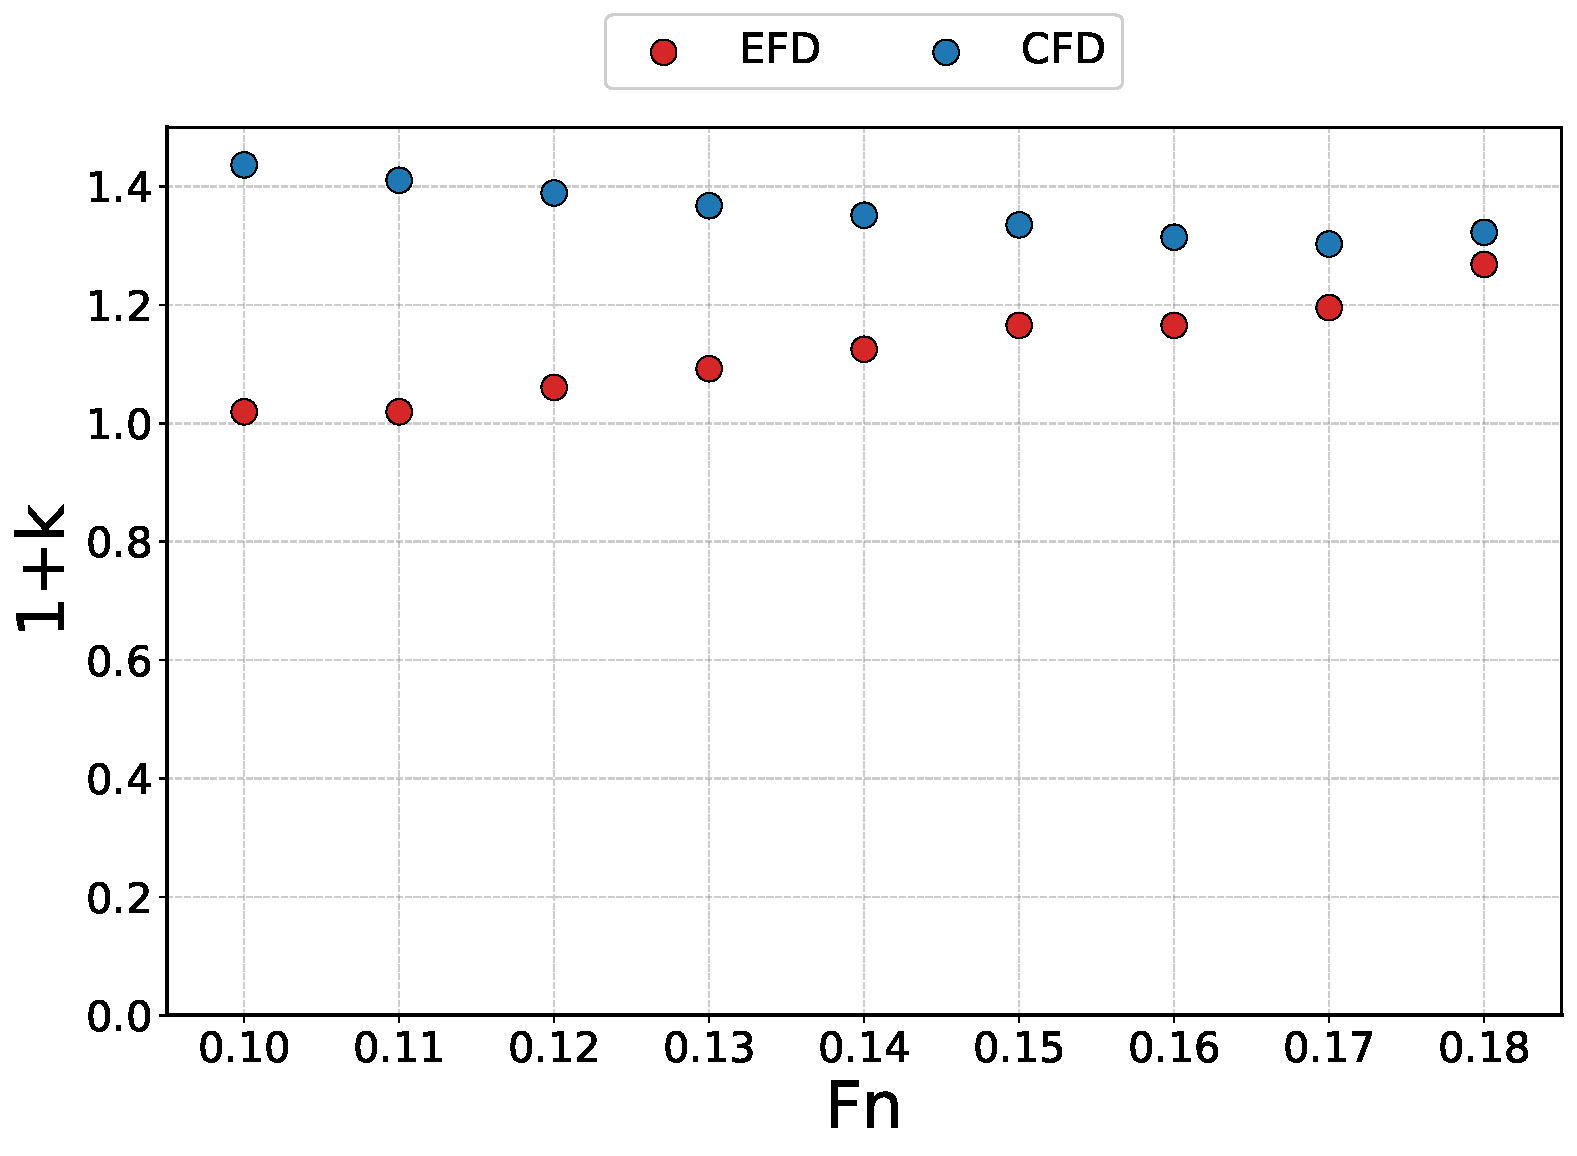
\includegraphics[width=\textwidth]{images/efd_cfd_form_factor_tpa_180_range}
         \caption{Calado 2.}
         \label{fig:efd_cfd_180_tpa_range}
     \end{subfigure}
     
     \vspace{0.5cm}
     
     \begin{subfigure}[b]{0.48\textwidth}
         \centering
         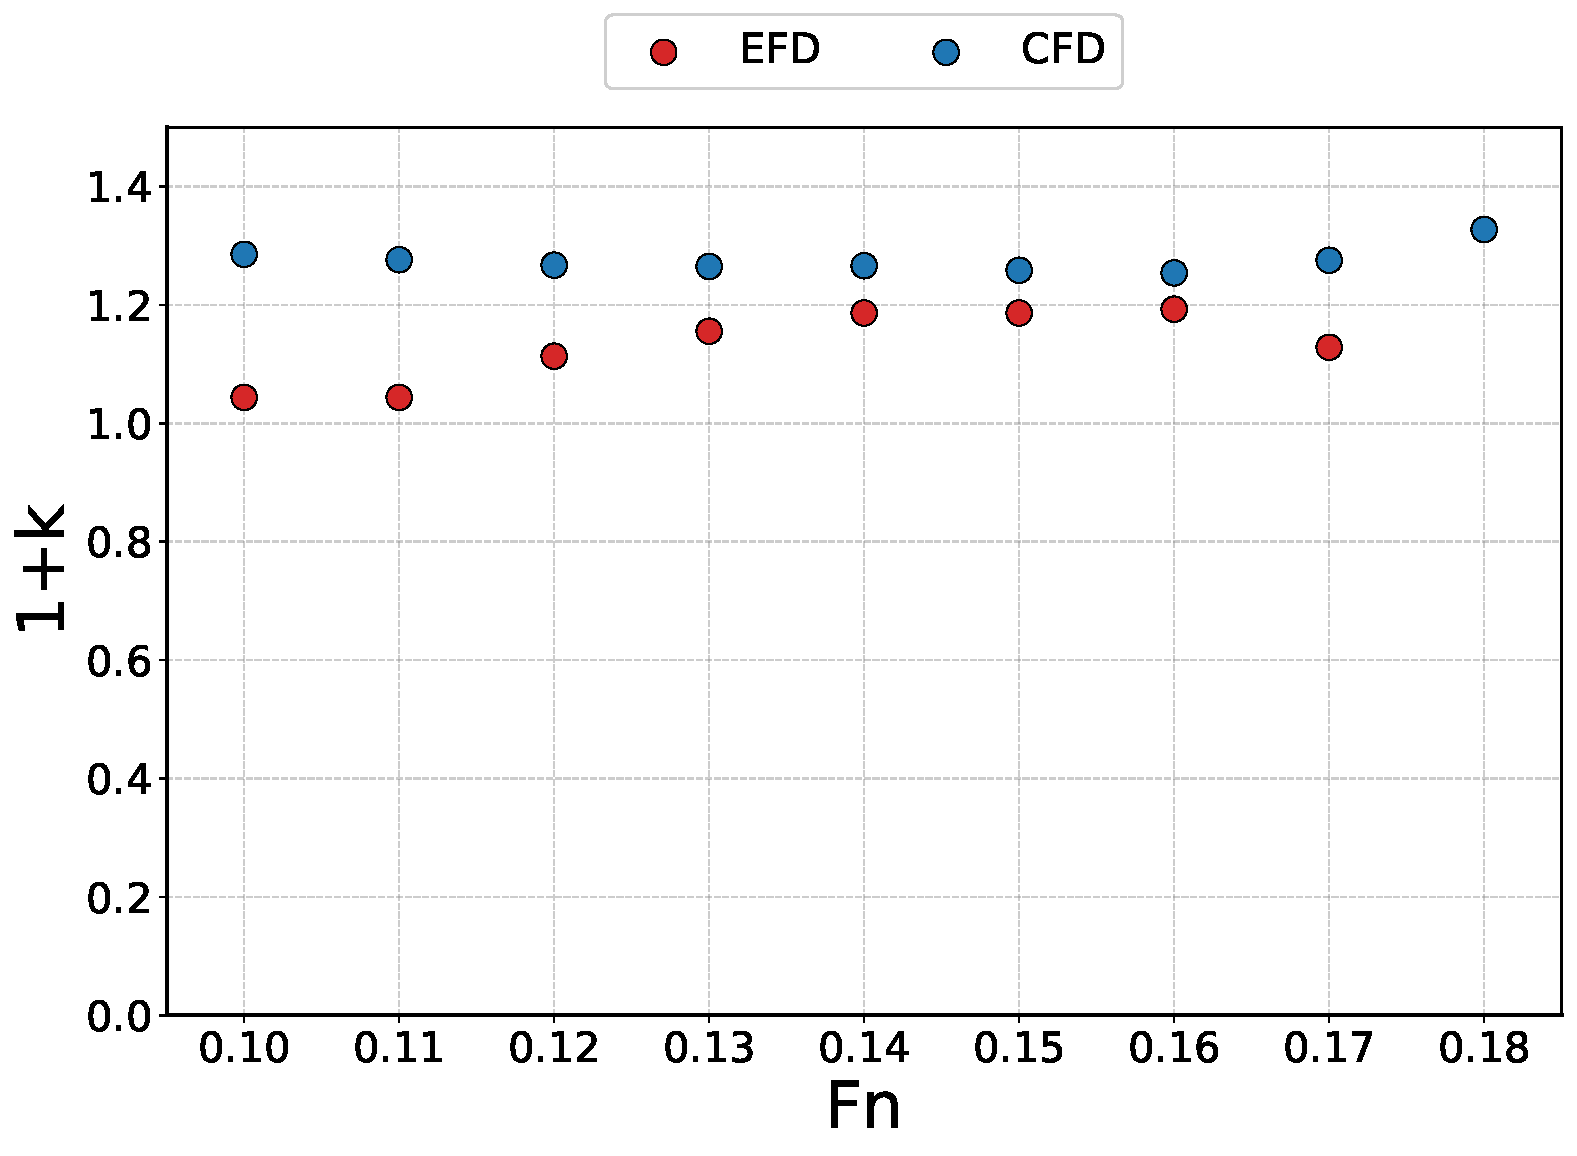
\includegraphics[width=\textwidth]{images/efd_cfd_form_factor_tpa_195_range}
         \caption{Calado 3.}
         \label{fig:efd_cfd_195_tpa_range}
     \end{subfigure}
     
     \caption{Variación del factor de forma $(1+k)$ del \textit{P1}, obtenido 
     mediante el método de Prohaska a partir de EFD y CFD, en función del 
     límite inferior del rango de Froude considerado en el ajuste.}
     \label{fig:comparativa_form_factor_range}
\end{figure}

Habiendo establecido un valor único y consistente de $(1+k)$ mediante Prohaska, 
surge la pregunta de cómo se relaciona este valor con los resultados obtenidos 
mediante el método de doble cuerpo, presentado en la 
Sección~\ref{sec:doble_cuerpo}. La Figura~\ref{fig:comparativa_doble_cuerpo} 
superpone, para cada calado, el valor adoptado por Prohaska (línea horizontal 
roja) con la evolución de $(1+k)$ obtenida mediante doble cuerpo en función 
de $Fr$ (puntos azules). Se observa que el valor de Prohaska coincide con los 
resultados de doble cuerpo específicamente en el rango $0.10 < Fr < 0.20$, es 
decir, el mismo rango utilizado para el ajuste de Prohaska. Sin embargo, para 
$Fr > 0.20$, el valor de doble cuerpo continúa creciendo de manera sostenida, 
mientras que el valor de Prohaska permanece constante por definición. Esto 
sugiere que el método de Prohaska, al restringirse a un rango acotado de bajas 
velocidades, podría estar capturando únicamente un punto particular de una 
curva de $(1+k)$ que en realidad varía con $Fr$ (o $Re$) en todo el rango 
operativo del buque, comportamiento que ya fue observado para el KCS y que 
será analizado en profundidad en la Sección~\ref{sec:analisis_efectos_escala}.

\begin{figure}[H]
     \centering
     \begin{subfigure}[b]{0.48\textwidth}
         \centering
         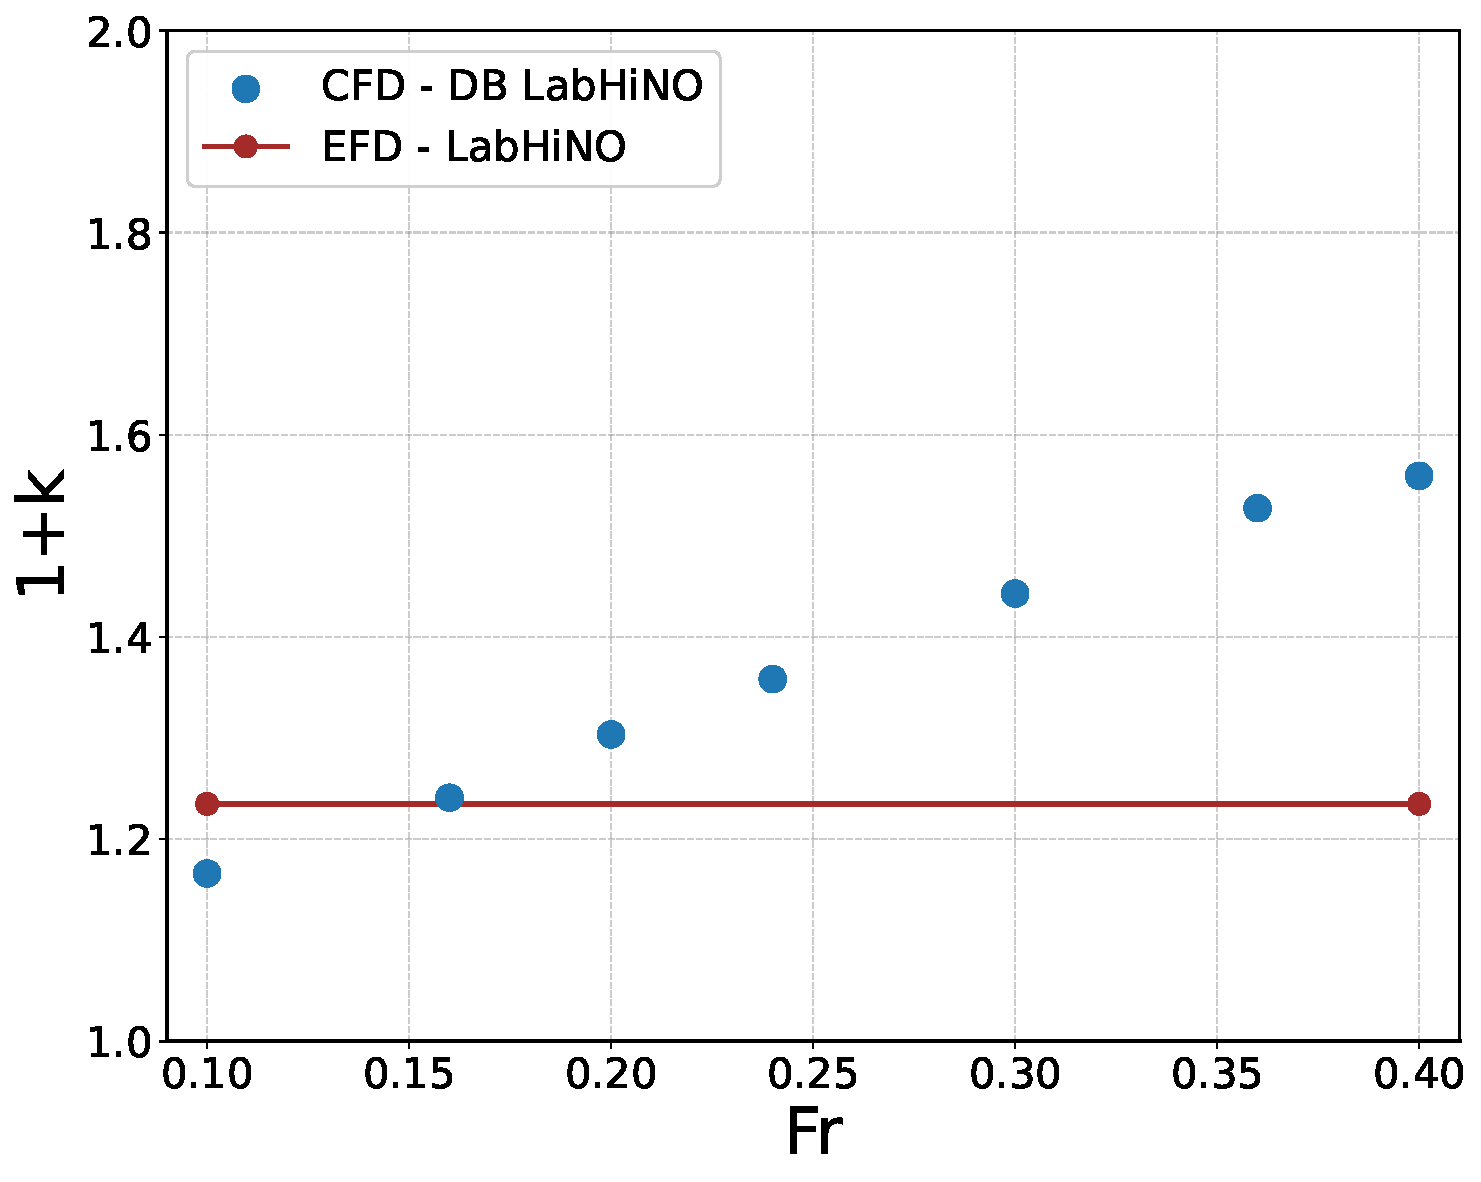
\includegraphics[width=\textwidth]{images/tpa_CFD_DB_prohaska_165.pdf}
         \caption{Calado 1.}
         \label{fig:tpa_proj_DB_k_escala20_165}
     \end{subfigure}
     \hfill
     \begin{subfigure}[b]{0.48\textwidth}
         \centering
         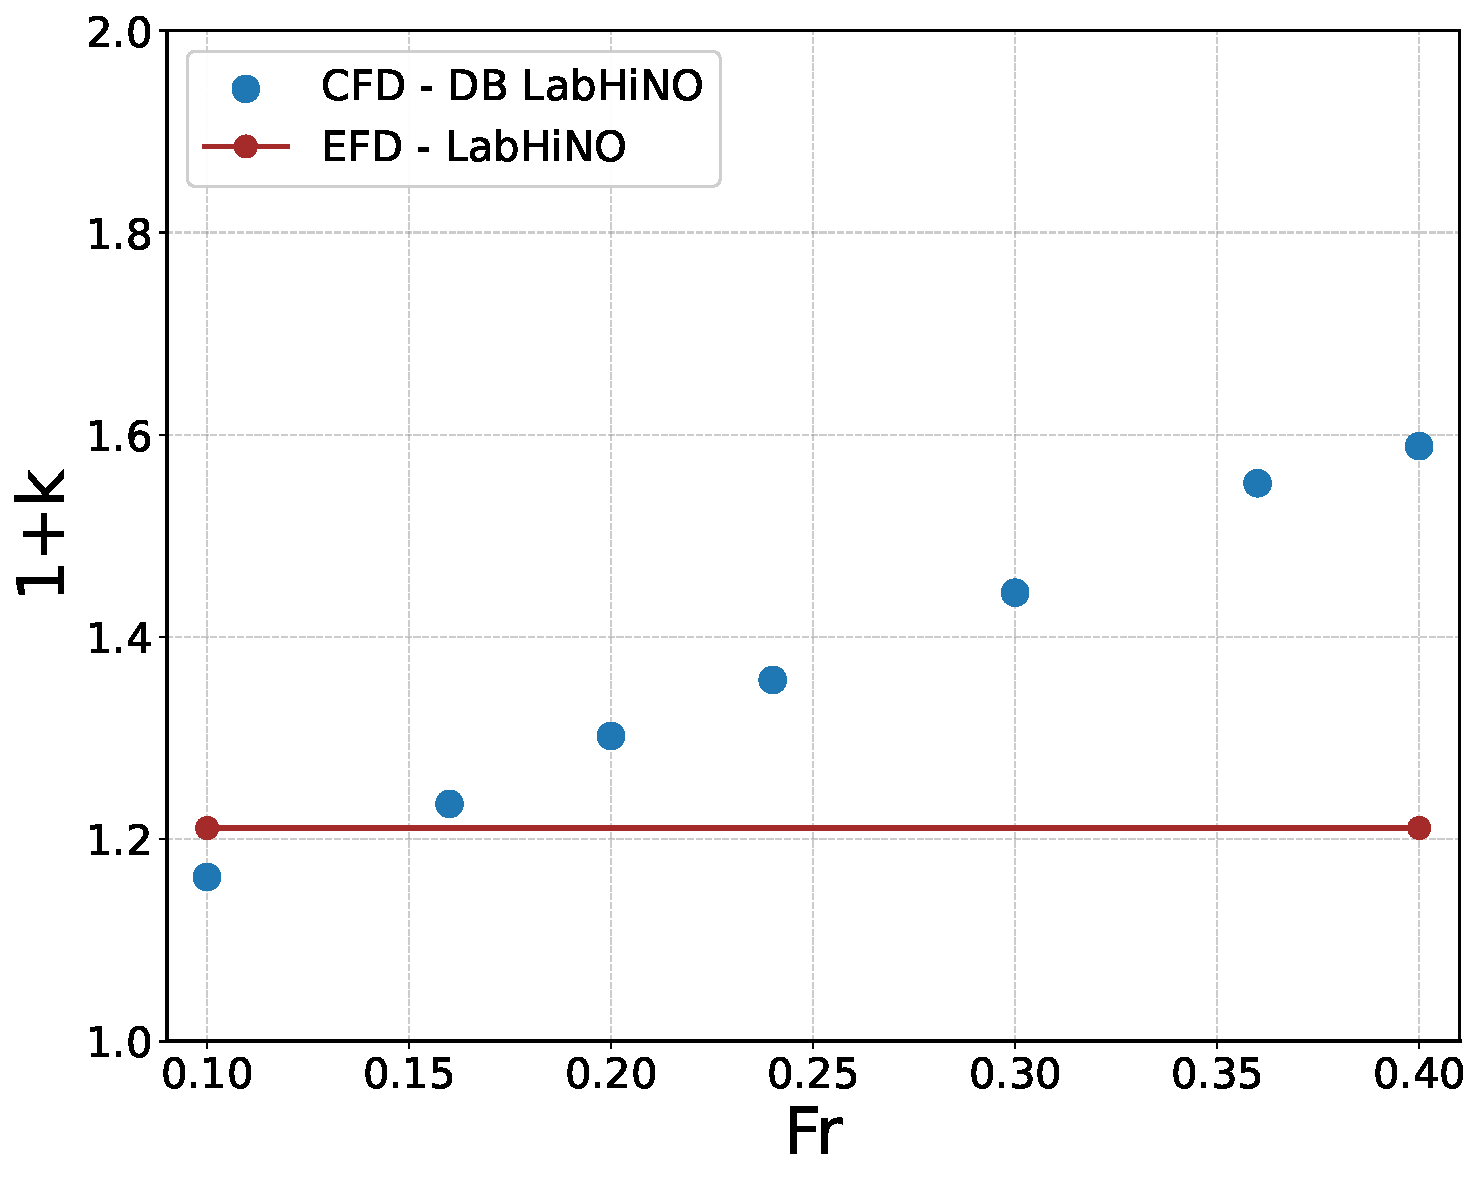
\includegraphics[width=\textwidth]{images/tpa_CFD_DB_prohaska_180.pdf}
         \caption{Calado 2.}
         \label{fig:tpa_proj_DB_k_escala20_180}
     \end{subfigure}
     
     \vspace{0.5cm}
     
     \begin{subfigure}[b]{0.48\textwidth}
         \centering
         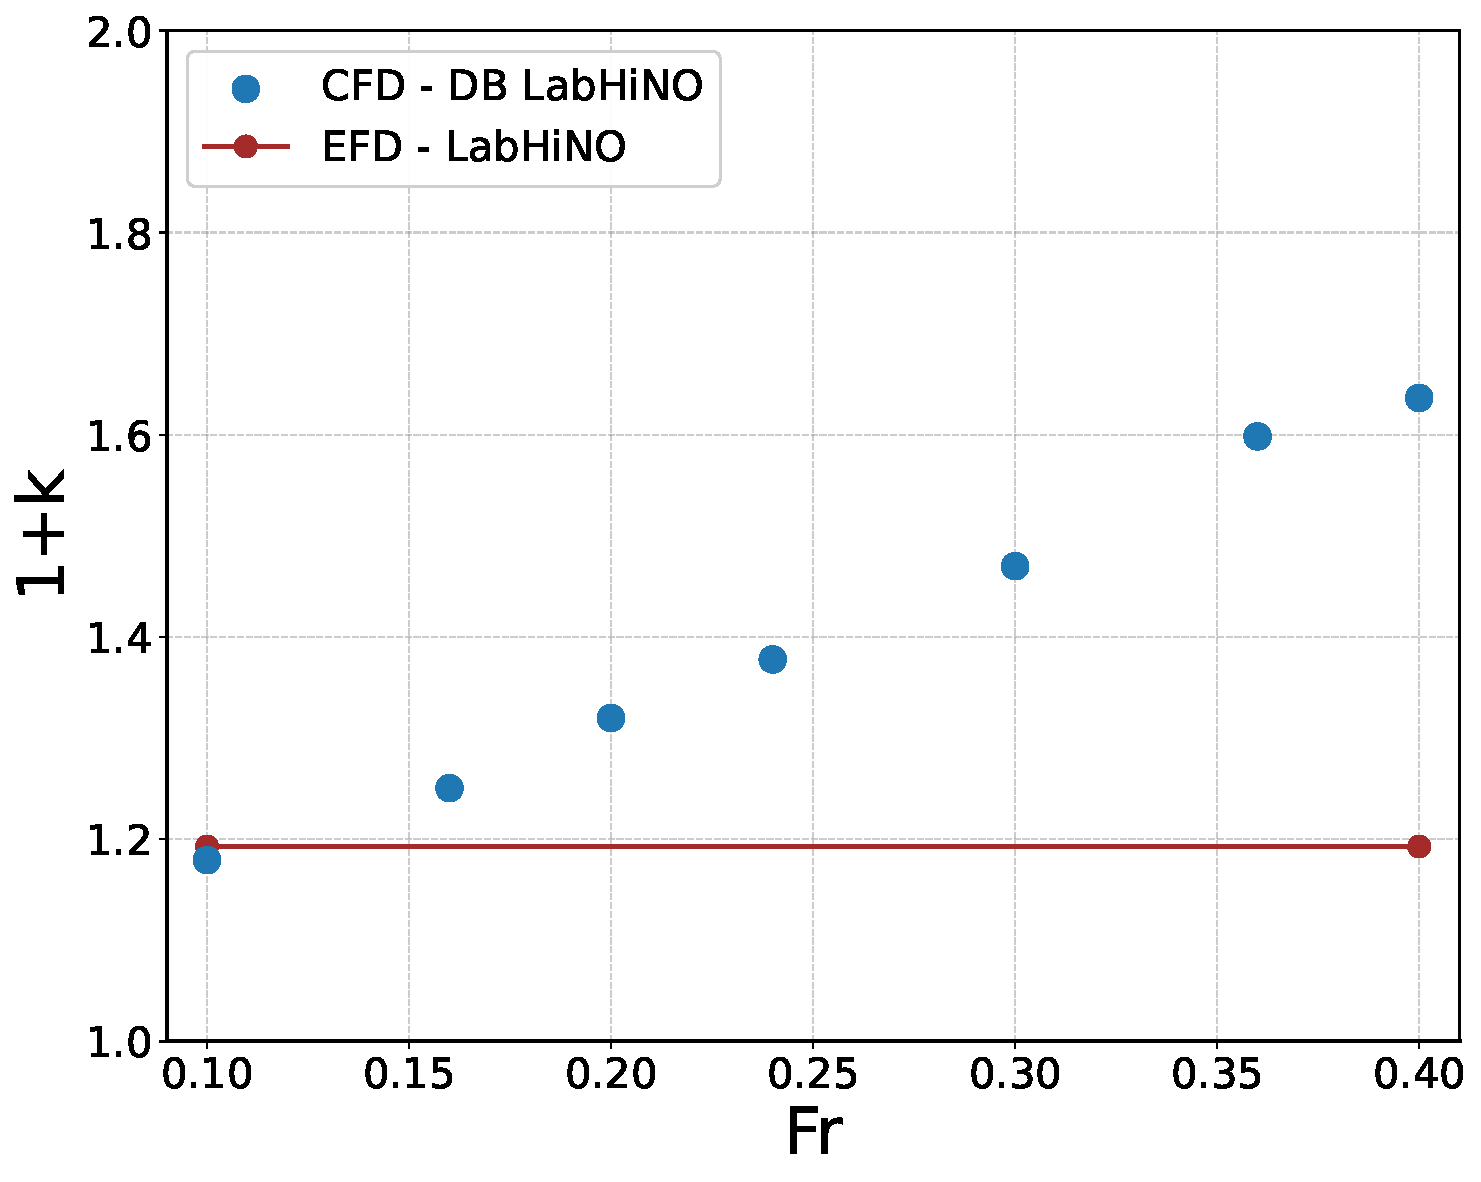
\includegraphics[width=\textwidth]{images/tpa_CFD_DB_prohaska_195.pdf}
         \caption{Calado 3.}
         \label{fig:tpa_proj_DB_k_escala20_195}
     \end{subfigure}
     
     \caption{Comparación del valor de $(1+k)$ adoptado por Prohaska (EFD/CFD, 
     línea roja) con la evolución de $(1+k)$ obtenida mediante el método de 
     doble cuerpo (puntos azules) en función de $Fr$, para los tres calados 
     del \textit{P1}.}
     \label{fig:comparativa_doble_cuerpo}
\end{figure}

\subsection{Discusión de incertidumbres y diferencias entre EFD y CFD}

Los resultados presentados hasta el momento permiten realizar una primera discusión conjunta sobre las incertidumbres involucradas y las diferencias observadas entre los ensayos experimentales (EFD) y las simulaciones numéricas (CFD) en la determinación de la resistencia al avance y del factor de forma $(1+k)$.

Desde el punto de vista experimental, la campaña realizada en el canal del LabHiNO mostró un nivel de repetibilidad adecuado y valores de incertidumbre combinada compatibles con las recomendaciones de la ITTC, especialmente en el rango de velocidades de interés operativo. Las curvas de resistencia obtenidas para los distintos calados presentan una evolución continua y físicamente consistente, lo que indica una correcta adquisición de la fuerza de remolque y una adecuada calibración del sistema de medición. No obstante, como es habitual en este tipo de ensayos, las mayores incertidumbres relativas se concentran en el rango de bajas velocidades, donde la resistencia total es pequeña y el método de Prohaska resulta particularmente sensible a pequeñas variaciones en $C_T$.

En este contexto, la aplicación del método de Prohaska a los datos experimentales evidenció desviaciones respecto de la linealidad teórica esperada, principalmente a bajos números de Froude. Tal comportamiento puede atribuirse a una combinación de factores: laminarización parcial del flujo, transición temprana, fenómenos viscosos locales asociados a la geometría del casco y limitaciones inherentes al uso de la línea de correlación ITTC-1957 en regímenes de Reynolds moderados. Estas desviaciones introducen una incertidumbre adicional en la estimación de $(1+k)$, que obliga a seleccionar cuidadosamente el rango de velocidades utilizado para la regresión lineal.

Las simulaciones CFD bifásicas reprodujeron de manera satisfactoria las curvas de resistencia total obtenidas experimentalmente en un amplio rango de velocidades, lo que constituye una primera validación global del modelo numérico. Las pequeñas diferencias observadas a velocidades elevadas pueden explicarse por diferencias en las condiciones de contorno dinámicas del casco, dado que en los ensayos experimentales se permitió el libre movimiento vertical y de cabeceo, mientras que en las simulaciones el casco se mantuvo fijo. En cualquier caso, estas discrepancias aparecen fuera del rango de operación típico del buque y no afectan las conclusiones principales.

En cuanto a la determinación del factor de forma mediante CFD, la aplicación directa del método de Prohaska mostró nuevamente desviaciones respecto de la recta teórica, aunque con una curvatura de signo opuesto a la observada experimentalmente. Esta diferencia pone de manifiesto una limitación conocida de los modelos RANS convencionales, que asumen flujo plenamente turbulento incluso en regímenes donde el flujo real se encuentra en transición. En consecuencia, tanto en EFD como en CFD, los puntos correspondientes a bajas velocidades no cumplen estrictamente los supuestos fundamentales del método de Prohaska, aunque por razones físicas y numéricas distintas.

La comparación sistemática entre EFD y CFD mostró que, al restringir el 
análisis a un rango adecuado de números de Froude, los valores de $(1+k)$ 
obtenidos por ambos enfoques mediante el método de Prohaska convergen de 
manera satisfactoria. Este resultado confirma que las discrepancias iniciales 
no responden a errores sistemáticos de medición o modelado, sino a la 
violación de los supuestos del método de Prohaska fuera de su rango óptimo de 
aplicación. La adopción de un intervalo reducido y físicamente consistente 
permitió reducir significativamente la dispersión y obtener valores 
comparables entre ambos enfoques.

Por último, la comparación entre el método de Prohaska (experimental y 
numérico) y el enfoque de doble cuerpo introdujo un nuevo elemento de análisis. 
Los valores de $(1+k)$ obtenidos mediante simulaciones de doble cuerpo, sin 
superficie libre, presentan una variación apreciable con la velocidad, lo que 
plantea interrogantes sobre la hipótesis de constancia del factor de forma 
asumida por el método de Prohaska. La superposición parcial entre los valores 
adoptados por Prohaska y el rango de resultados del método de doble cuerpo 
sugiere que ambos enfoques capturan distintos aspectos del mismo fenómeno 
viscoso, aunque con sensibilidades diferentes al régimen de flujo y al 
modelado de la turbulencia.

En síntesis, los resultados obtenidos hasta acá indican que:
\begin{itemize}
    \item Las mediciones experimentales presentan niveles de incertidumbre 
    compatibles con estándares internacionales y constituyen una base 
    confiable para la validación numérica.
    \item El método de Prohaska es altamente sensible a las condiciones de 
    flujo a bajas velocidades, tanto en EFD como en CFD, lo que exige una 
    selección cuidadosa del rango de aplicación.
    \item Las simulaciones CFD con superficie libre reproducen adecuadamente 
    la resistencia total, pero introducen limitaciones adicionales en 
    regímenes transicionales debido a las hipótesis del modelo de turbulencia.
    \item La concordancia entre EFD y CFD mejora significativamente cuando se 
    restringe el análisis a rangos donde los supuestos físicos del método de 
    Prohaska son razonablemente válidos.
\end{itemize}

Estas observaciones establecen un marco sólido para los análisis posteriores, 
donde se profundizará en la descomposición de la resistencia viscosa y en la 
interpretación física de las variaciones de $(1+k)$ con la velocidad 
observadas mediante el método de doble cuerpo.

\subsection{Análisis de efectos de escala} \label{sec:analisis_efectos_escala}

\paragraph{Extensión de escalas}

Con el fin de resaltar el comportamiento distintivo de $(1+k)$ en función de 
$Re$ que se ha encontrado para el \textit{P1}, en esta subsección se compara 
dicho comportamiento con el correspondiente al KCS. A diferencia de las 
secciones anteriores, donde $(1+k)$ se presentó en función de $Fr$ para un 
único buque a una escala fija, aquí se opta por graficar en función de $Re$, 
dado que esta variable permite comparar directamente resultados provenientes 
de buques y escalas distintas (KCS a 1:79 y 1:75, y \textit{P1} a 1:20) en un 
mismo eje, algo que $Fr$ no posibilita al depender únicamente de la velocidad 
relativa a la eslora de cada modelo.

En primer lugar, con el propósito de una mayor claridad analítica, los 
resultados presentados en las Figuras~\ref{fig:k_195} y \ref{fig:kcs_DB_prohaska} 
se reúnen en la Figura~\ref{fig:comparacion_total_kcs_tpa}.

La Figura~\ref{fig:comparacion_total_kcs_tpa} muestra los valores de $(1+k)$ 
frente a $Re$ obtenidos mediante CFD \textit{double body} (DB) para el KCS 
a escala 1:79, el KCS a escala 1:75 de \citet{TERZIEV2021147} y el \textit{P1} 
en escala modelo (1:20) para el Calado~3. El gráfico incluye además los 
valores experimentales (EFD) de $(1+k)$ determinados mediante el método de 
Prohaska en el presente trabajo, para el KCS a escala 1:79 y para el 
\textit{P1}.

\begin{figure}[htpb]
	\centering
	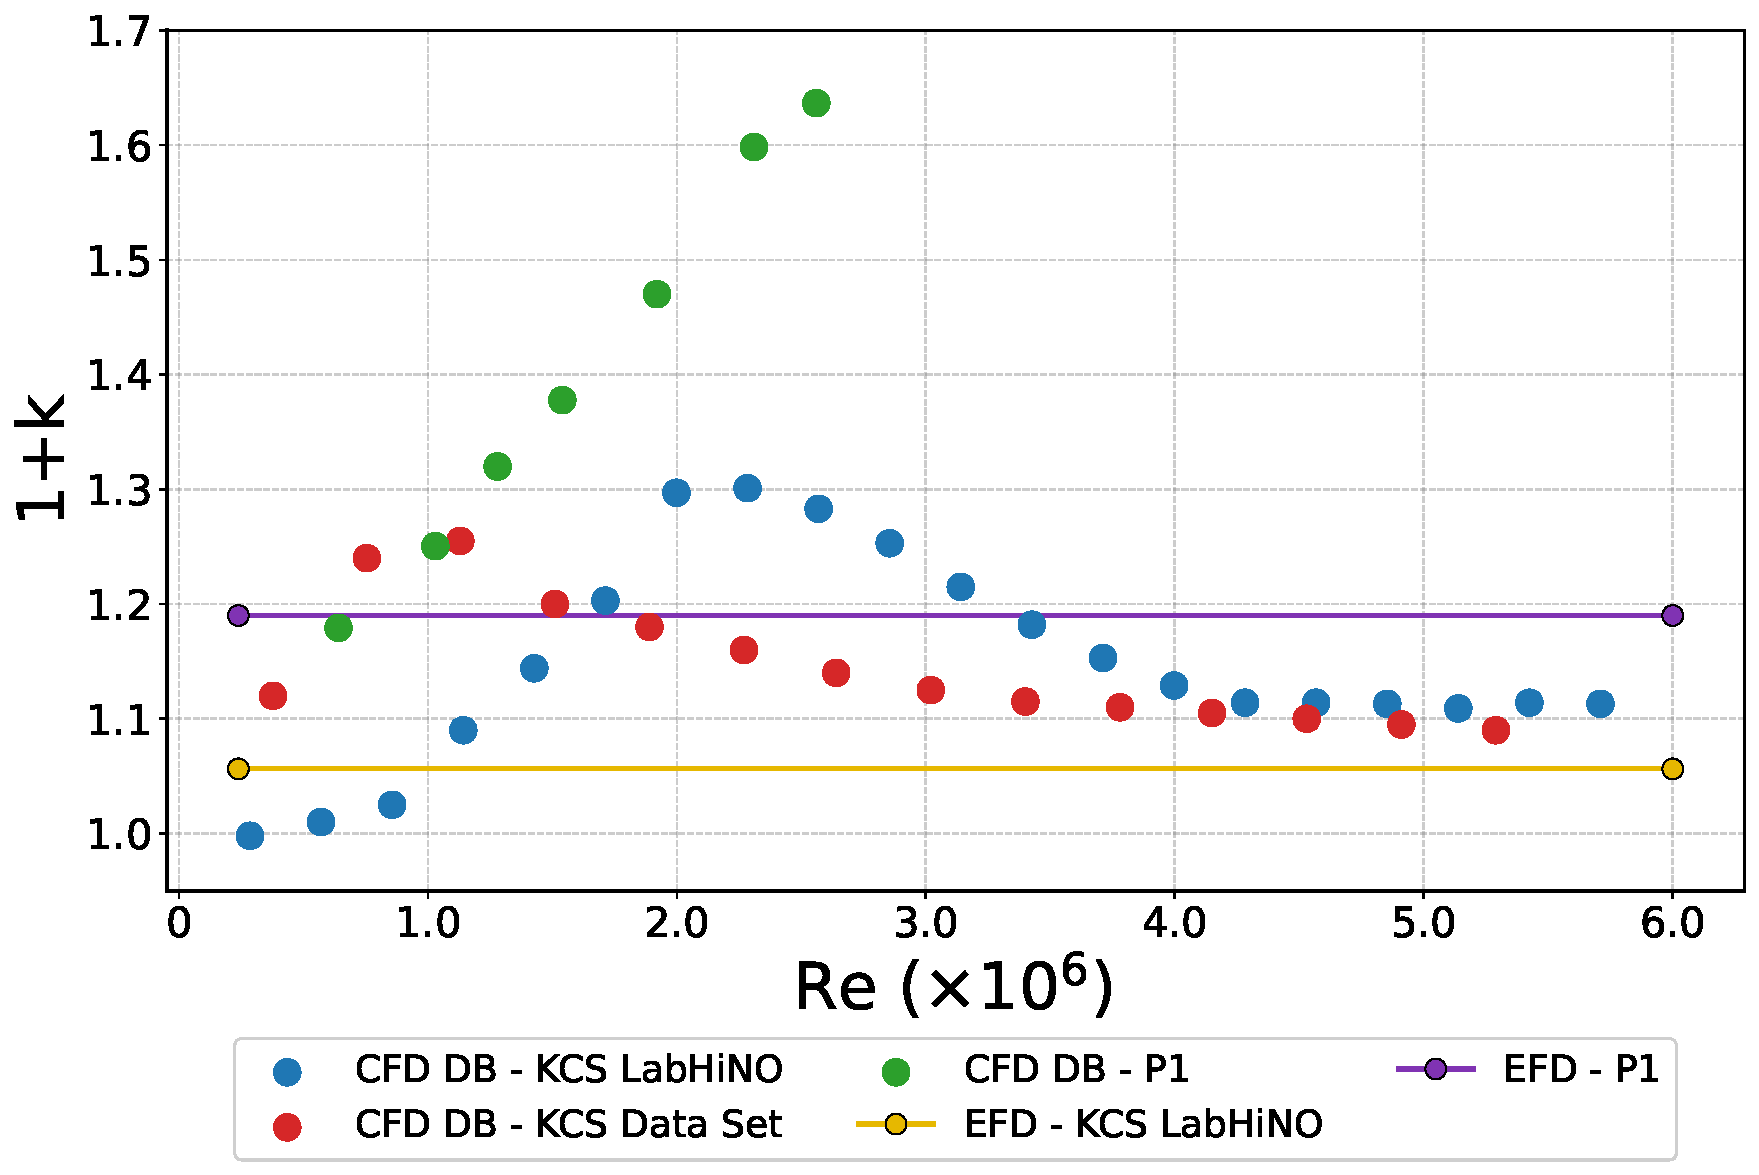
\includegraphics[width=.6\columnwidth]{images/comparacion_total_kcs_tpa.pdf}
	\caption{$(1+k)$ frente a $Re$ para el KCS (CFD DB, escalas 1:79 y 1:75 
	de \citet{TERZIEV2021147}, y EFD a 1:79) y para el \textit{P1} (CFD DB y 
	EFD, escala 1:20, Calado~3).}
	\label{fig:comparacion_total_kcs_tpa}
\end{figure}

Es evidente que, dentro del rango de velocidades del modelo considerado, el 
\textit{P1} no alcanza un valor asintótico de $(1+k)$, a diferencia de lo 
observado en el KCS. Por consiguiente, y en contraste con el comportamiento 
mostrado por el KCS, el valor de $(1+k)$ del \textit{P1} calculado mediante 
CFD DB se desvía progresivamente del valor obtenido por el método de 
Prohaska, ya sea numérica o experimentalmente, a medida que aumenta la 
velocidad del modelo.

Para comprender mejor el comportamiento de $(1+k)$ en función de $Re$ en el 
caso del \textit{P1}, se realizaron cálculos CFD DB de $(1+k)$ para diferentes 
escalas de modelo, con el fin de abarcar un rango más amplio de $Re$. Se 
evaluaron la escala 1:20 (ya presentada) y tres escalas adicionales, 1:10, 
1:5 y 1:1.

\begin{figure}[htpb]
	\centering
	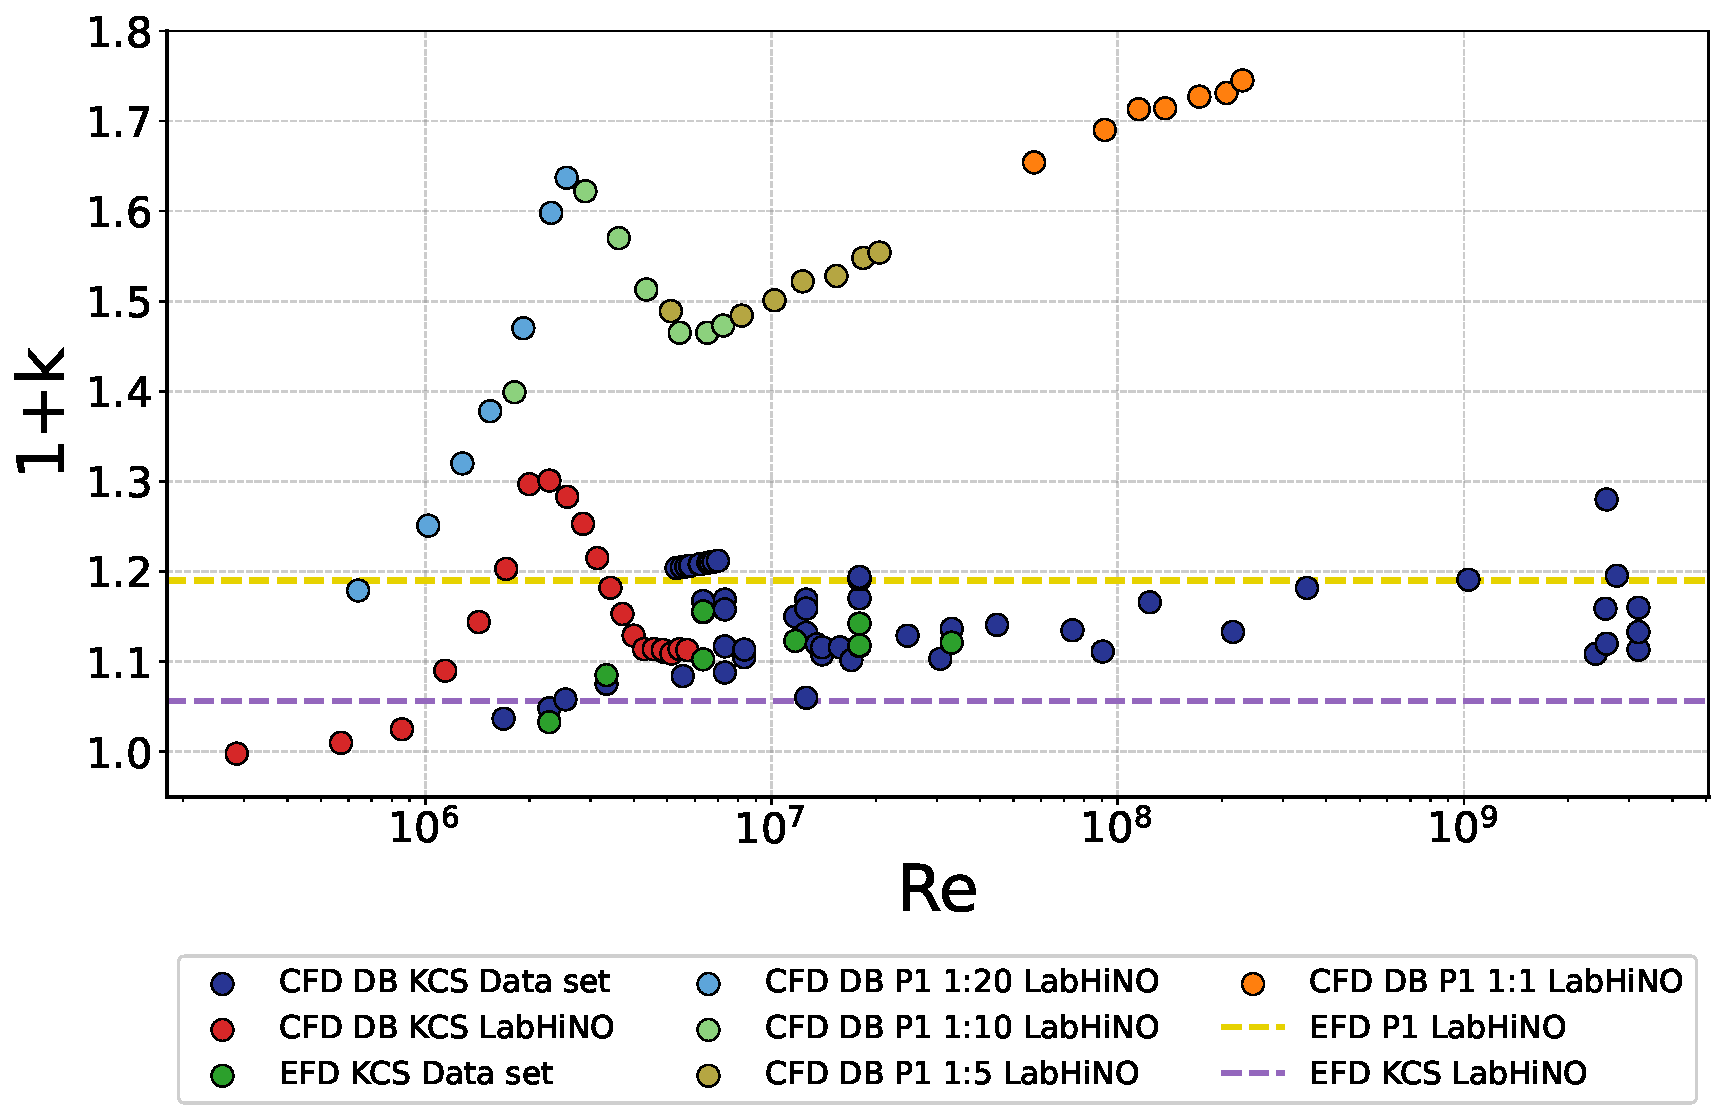
\includegraphics[width=.6\columnwidth]{images/completo_log_kcs_lit_tpa.pdf}
	\caption{$(1+k)$ frente a $Re$ para el KCS y el \textit{P1}, en escala 
	logarítmica. Para el KCS se muestran los resultados propios obtenidos en 
	el LabHiNO (CFD DB y Prohaska EFD, escala 1:79) junto con el conjunto de 
	datos recopilado por \citet{TerzievDataSet} (CFD DB y Prohaska, otras 
	escalas y laboratorios). Para el \textit{P1} se muestran únicamente 
	resultados propios: CFD DB en las escalas 1:20, 1:10, 1:5 y 1:1, y el 
	valor experimental obtenido por Prohaska en el LabHiNO (escala 1:20).}
	\label{fig:comparacion_total_escalas_kcs_tpa}
\end{figure}

La Figura~\ref{fig:comparacion_total_escalas_kcs_tpa} permite contextualizar 
los resultados del \textit{P1} dentro de la tendencia general documentada para 
el KCS en la literatura, y extender el análisis del \textit{P1} a un rango 
más amplio de $Re$ mediante simulaciones a distintas escalas geométricas.

Se observa que el modelo CFD DB presenta, para ambos buques estudiados, un 
pico aproximadamente en el mismo rango de $Re$. Como se mencionó previamente, 
este pico podría estar directamente asociado con la modelización de la 
transición.

Por otro lado, se observa en la Figura que la variación de $(1+k)$ con $Re$ 
disminuye para el KCS a valores altos de $Re$, mientras que para el 
\textit{P1} la tendencia creciente persiste hasta la escala buque (1:1), sin 
alcanzar un valor asintótico dentro del rango analizado.

El impacto de $Re$ sobre el valor de $(1+k)$ es considerablemente más 
pronunciado en el \textit{P1}. A modo ilustrativo, la diferencia entre el 
valor de $(1+k)$ a bajo $Re$ y a alto $Re$ es aproximadamente del 40\% para 
el \textit{P1}, mientras que para el KCS es cercana al 8\%. Además, el valor 
final de $(1+k)$ del \textit{P1} resulta casi un 50\% superior al del KCS, 
valor no encontrado en la literatura de hidrodinámica naval al día de hoy.

Para verificar que este comportamiento no es exclusivo del \textit{P1}, 
se extendió el análisis CFD DB a los otros dos pesqueros analizados en 
esta tesis (\textit{P2}, $L/B = 3{.}23$; \textit{P3}, $L/B = 2{.}85$). 
La Figura~\ref{fig:Re_formfactor} muestra la evolución de $(1+k)$ con 
$Re$ para los cuatro cascos. Los tres pesqueros presentan el mismo 
comportamiento creciente y no asintótico observado en el \textit{P1}, en 
marcado contraste con la estabilización del KCS. Esta consistencia 
confirma que la falta de valor asintótico de $(1+k)$ no es una 
singularidad del \textit{P1}, sino una característica común a los 
pesqueros estudiados. Las causas geométricas de este comportamiento se 
analizan en profundidad en la Sección~\ref{sec:generalizacion_LB}.

\begin{figure}[htpb]
    \centering
    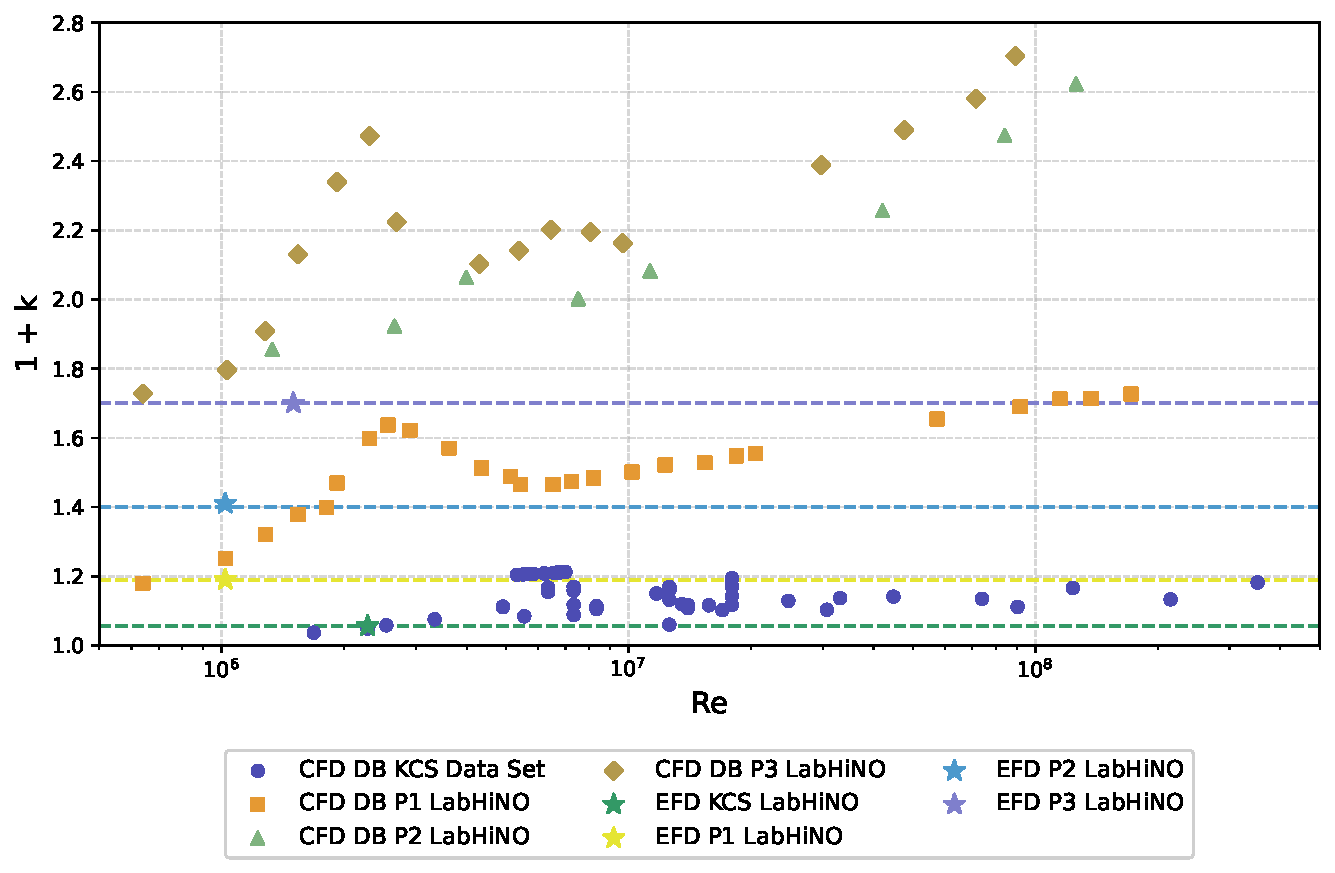
\includegraphics[width=.6\textwidth]{./images/completo_log_kcs_lit_tpa_jpa_contessi.pdf}
    \caption{Evolución de $(1+k)$ con el número de Reynolds para el KCS 
    y los tres pesqueros analizados.}
    \label{fig:Re_formfactor}
\end{figure}

El método de \citet{gomezgarcia} (Sección~\ref{sec:factor_de_forma_antec})
ofrece una prueba cuantitativa directa de cuán anómalo resulta el
comportamiento del \textit{P1}. Aplicando su relación empírica
[Ecuación~\eqref{eq:gomezgarcia}] a la escala del modelo ($\lambda = 20$), el efecto de escala predicho es $K_S - K_M \approx 1{.}91\times 19\times 10^{-3}= 0{.}036$. El valor obtenido por CFD de doble cuerpo para el \textit{P1} en el Calado~3, en cambio, es $k_S - k_M = 0{.}716 - 0{.}194 = 0{.}522$, es decir, aproximadamente catorce veces mayor que la predicción. La fórmula de \citet{gomezgarcia}, calibrada para estimar la corrección de escala del factor de forma, subestima en más de un orden de magnitud el efecto de escala real de este casco.

Esta discrepancia no se limita a la magnitud, sino que alcanza a la propia
forma funcional. Al ajustar el modelo lineal de \citet{gomezgarcia} —$K_S -
K_M$ en función de $\lambda$— a los cuatro puntos de escala calculados para el \textit{P1} (1:20, 1:10, 1:5 y 1:1), la pendiente resultante es de
$15{.}8\times 10^{-3}$, más de ocho veces la de $1{.}851\times 10^{-3}$ de la regresión original (Figura~\ref{fig:gomez-garcia-nuestro}). Más significativo aún es que el ajuste lineal del \textit{P1} arroja una ordenada al origen de $0{.}054$, de modo que predice un efecto de escala espurio de $K_S - K_M \approx 0{.}070$ en $\lambda = 1$, condición en la que necesariamente debe anularse. La regresión de \citet{gomezgarcia}, en cambio, satisface esta restricción física ($K_S - K_M \approx 0{.}001$ en $\lambda = 1$). El modelo lineal, por lo tanto, no puede recuperarse reescalando la pendiente: la hipótesis de linealidad en $\lambda$ sobre la que se apoya no se cumple para esta clase de casco.

El origen de esta inaplicabilidad es geométrico. Las cuatro familias de
geosims sobre las que \citet{gomezgarcia} calibró su correlación corresponden a cascos esbeltos convencionales, con relaciones $L_{PP}/B$ comprendidas entre $6{.}98$ y $9{.}07$; ninguna se aproxima siquiera a la baja esbeltez del \textit{P1} ($L/B \approx 2{.}8$--$3{.}5$). La correlación se aplica, por lo tanto, fuera del dominio para el que fue derivada, en un régimen donde la resistencia por presión viscosa, despreciable en los cascos esbeltos de lamuestra original, pasa a ser una fracción dominante de la resistencia viscosa total, como se demuestra en la
Sección~\ref{sec:descomposicion_de_la_res_viscosa}.

\begin{figure}[htpb]
\centering
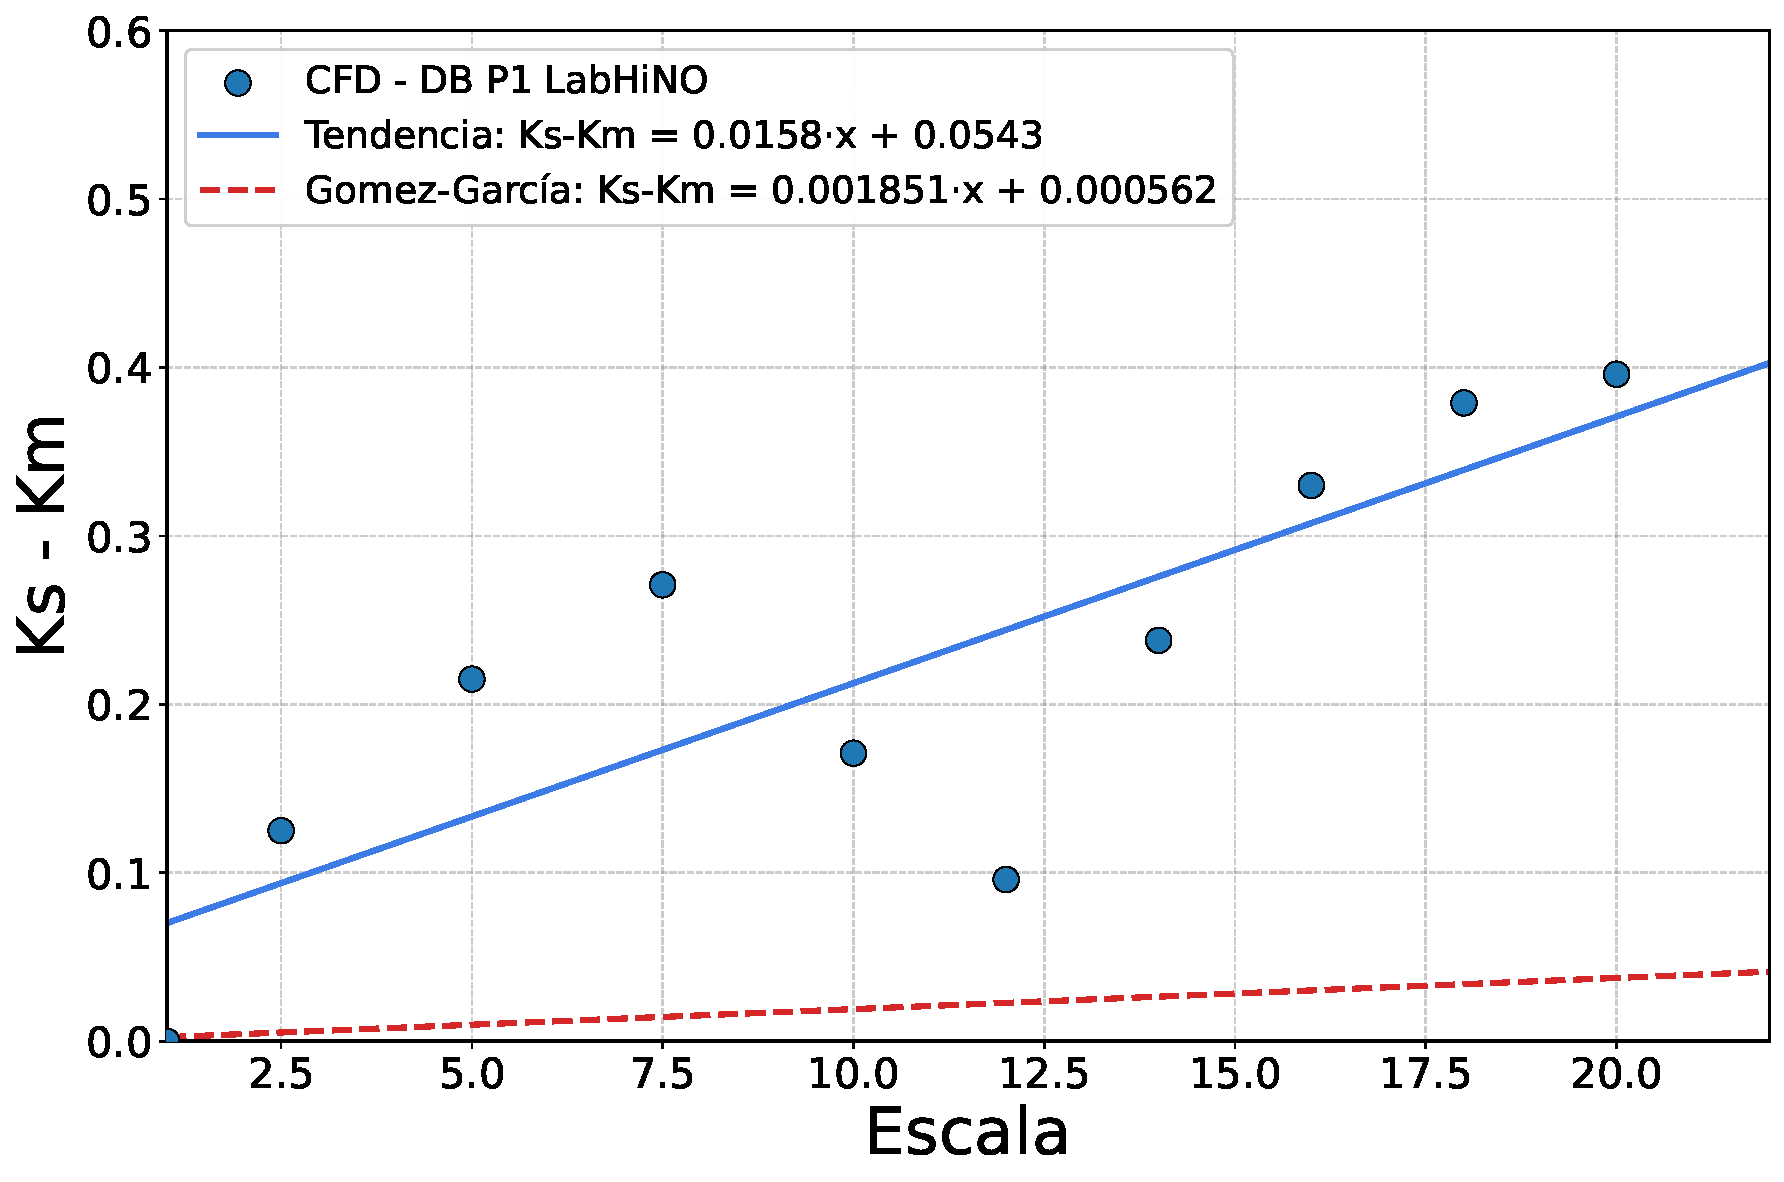
\includegraphics[width=0.6\textwidth]{images/gomez-garcia-nuestro.pdf}
\caption{Efecto de escala del factor de forma del \textit{P1}, $k_S - k_M$,
en función de la razón de escala $\lambda$, con la recta de regresión lineal ajustada a los puntos calculados por CFD de doble cuerpo. Se incluye, para comparación, la recta de \citet{gomezgarcia}.}
\label{fig:gomez-garcia-nuestro}
\end{figure}

De manera similar, el método de \citet{keh-sik-min} (Sección~\ref{sec:factor_de_forma_antec}) 
podría ser aplicado exitosamente al KCS, dado que se observa dicho factor de 
forma terminal a altos valores de $Re$, pero no así al \textit{P1}, donde 
$(1+k)$ no alcanza un valor asintótico dentro del rango analizado. Esto 
motiva la siguiente sección, donde se analizan las posibles razones de este 
aumento continuo del factor de forma.


\subsection{Descomposición de la resistencia viscosa} \label{sec:descomposicion_de_la_res_viscosa}

A diferencia del ensayo experimental, donde solo es posible medir la fuerza 
total de resistencia, la simulación CFD en configuración de doble cuerpo 
permite separar explícitamente las contribuciones friccional y de presión 
viscosa, lo que posibilita el análisis detallado que se presenta en esta 
sección. Esta descomposición se basa en la relación:
%
\begin{equation}
    (1+k) = \frac{C_V}{C_{F0}} = \frac{C_F + C_{PV}}{C_{F0}}
    \label{eq:descomposicion_1k}
\end{equation}
%
donde $C_F$ es el coeficiente de resistencia friccional, $C_{PV}$ el 
coeficiente de resistencia por presión viscosa y $C_{F0}$ el coeficiente de 
la línea de correlación ITTC-57. La Ecuación~\eqref{eq:descomposicion_1k} 
permite anticipar el comportamiento de $(1+k)$ con $Re$: si $C_{PV}$ 
disminuye con $Re$ más lentamente que $C_{F0}$ en el denominador, el 
cociente continúa creciendo aun cuando ambos coeficientes decaigan en 
términos absolutos.

La Figura~\ref{descomposicion_fuerzas} muestra el coeficiente de resistencia 
total ($C_T$), el coeficiente de resistencia friccional ($C_F$) y el 
coeficiente de resistencia por presión viscosa ($C_{PV}$) obtenidos a partir 
de la simulación CFD en configuración de doble cuerpo (DB) para el 
\textit{P1}, en función del número de Reynolds ($Re$). Asimismo, se incluye 
la línea de correlación ITTC-57 ($C_{F0}$) a efectos comparativos.

\begin{figure}
\centering
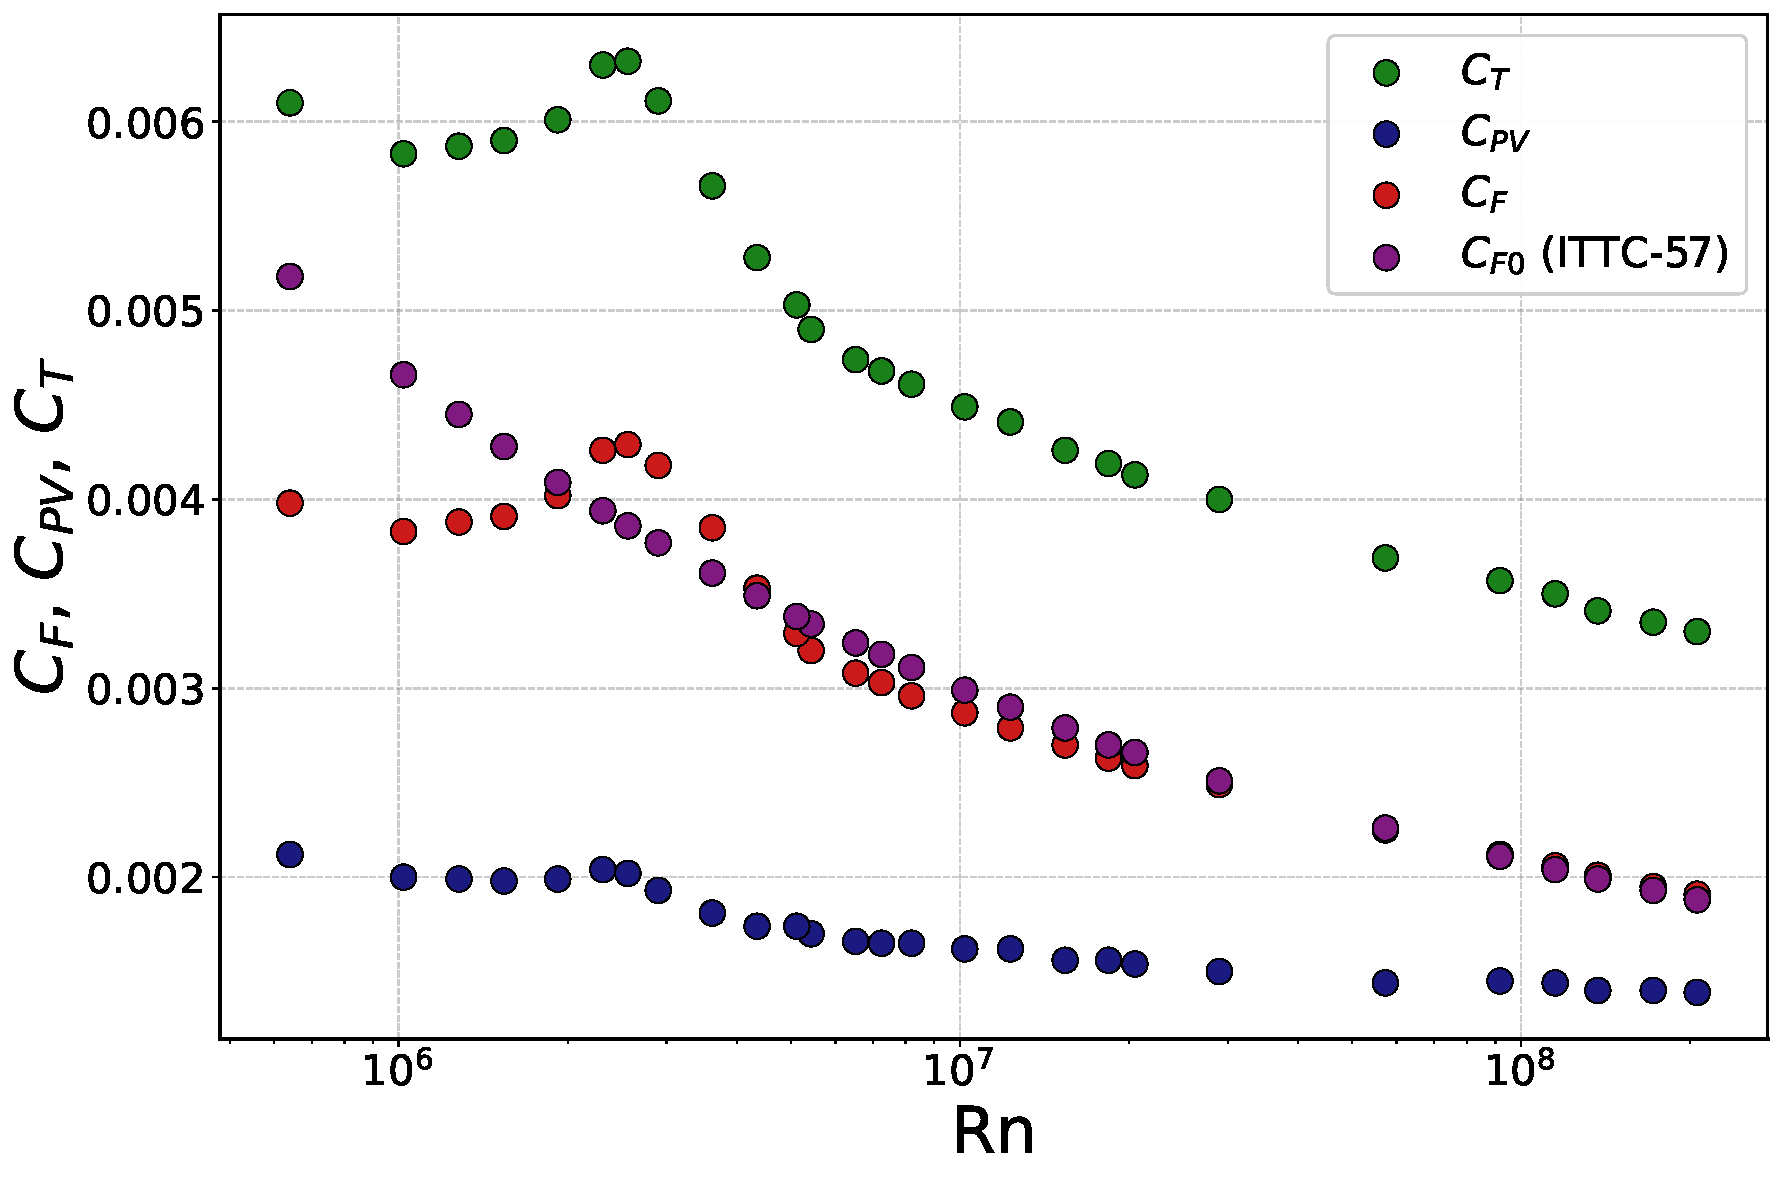
\includegraphics[width=.6\columnwidth]{./images/descomposicion_coeficientes.pdf}
\caption{Coeficientes $C_T$, $C_{PV}$ y $C_F$ obtenidos mediante CFD en 
configuración de doble cuerpo, junto con la línea ITTC-57 ($C_{F0}$), en 
función de $Re$ para el \textit{P1}.}
\label{descomposicion_fuerzas}
\end{figure}

El coeficiente de resistencia friccional ($C_F$) del modelo CFD-DB coincide 
estrechamente con la correlación ITTC-57 para valores de $Re$ mayores que 
$5\times 10^6$, es decir, más allá de la región de transición. En cambio, 
$C_{PV}$ disminuye de manera muy lenta con $Re$. Según la 
Ecuación~\eqref{eq:descomposicion_1k}, esta disminución lenta de $C_{PV}$ en 
el numerador, combinada con la disminución más rápida de $C_{F0}$ en el 
denominador, genera el incremento sostenido de $(1+k)$ observado. La tasa de 
crecimiento de $(1+k)$ con $Re$ disminuye a medida que aumenta $Re$, 
fundamentalmente debido a la meseta que alcanza $C_F$.

Para analizar el comportamiento característico de $C_{PV}$, la 
Figura~\ref{cpv_friccion} compara los valores de $C_F$ y $C_{PV}$ obtenidos 
para el \textit{P1} y para el KCS. Se observa que, en todo el rango de 
Reynolds considerado, el valor de $C_{PV}$ del \textit{P1} es sustancialmente 
superior al del KCS, y que dicha diferencia se mantiene prácticamente sin 
disminuir a medida que aumenta $Re$. Cualitativamente, mientras que en el 
KCS $C_F$ domina ampliamente sobre $C_{PV}$ en todo el rango analizado, en el 
\textit{P1} ambos coeficientes resultan de magnitud comparable, lo que indica 
que la presión viscosa constituye una fracción mucho más significativa de la 
resistencia viscosa total para este casco.

\begin{figure}
\centering
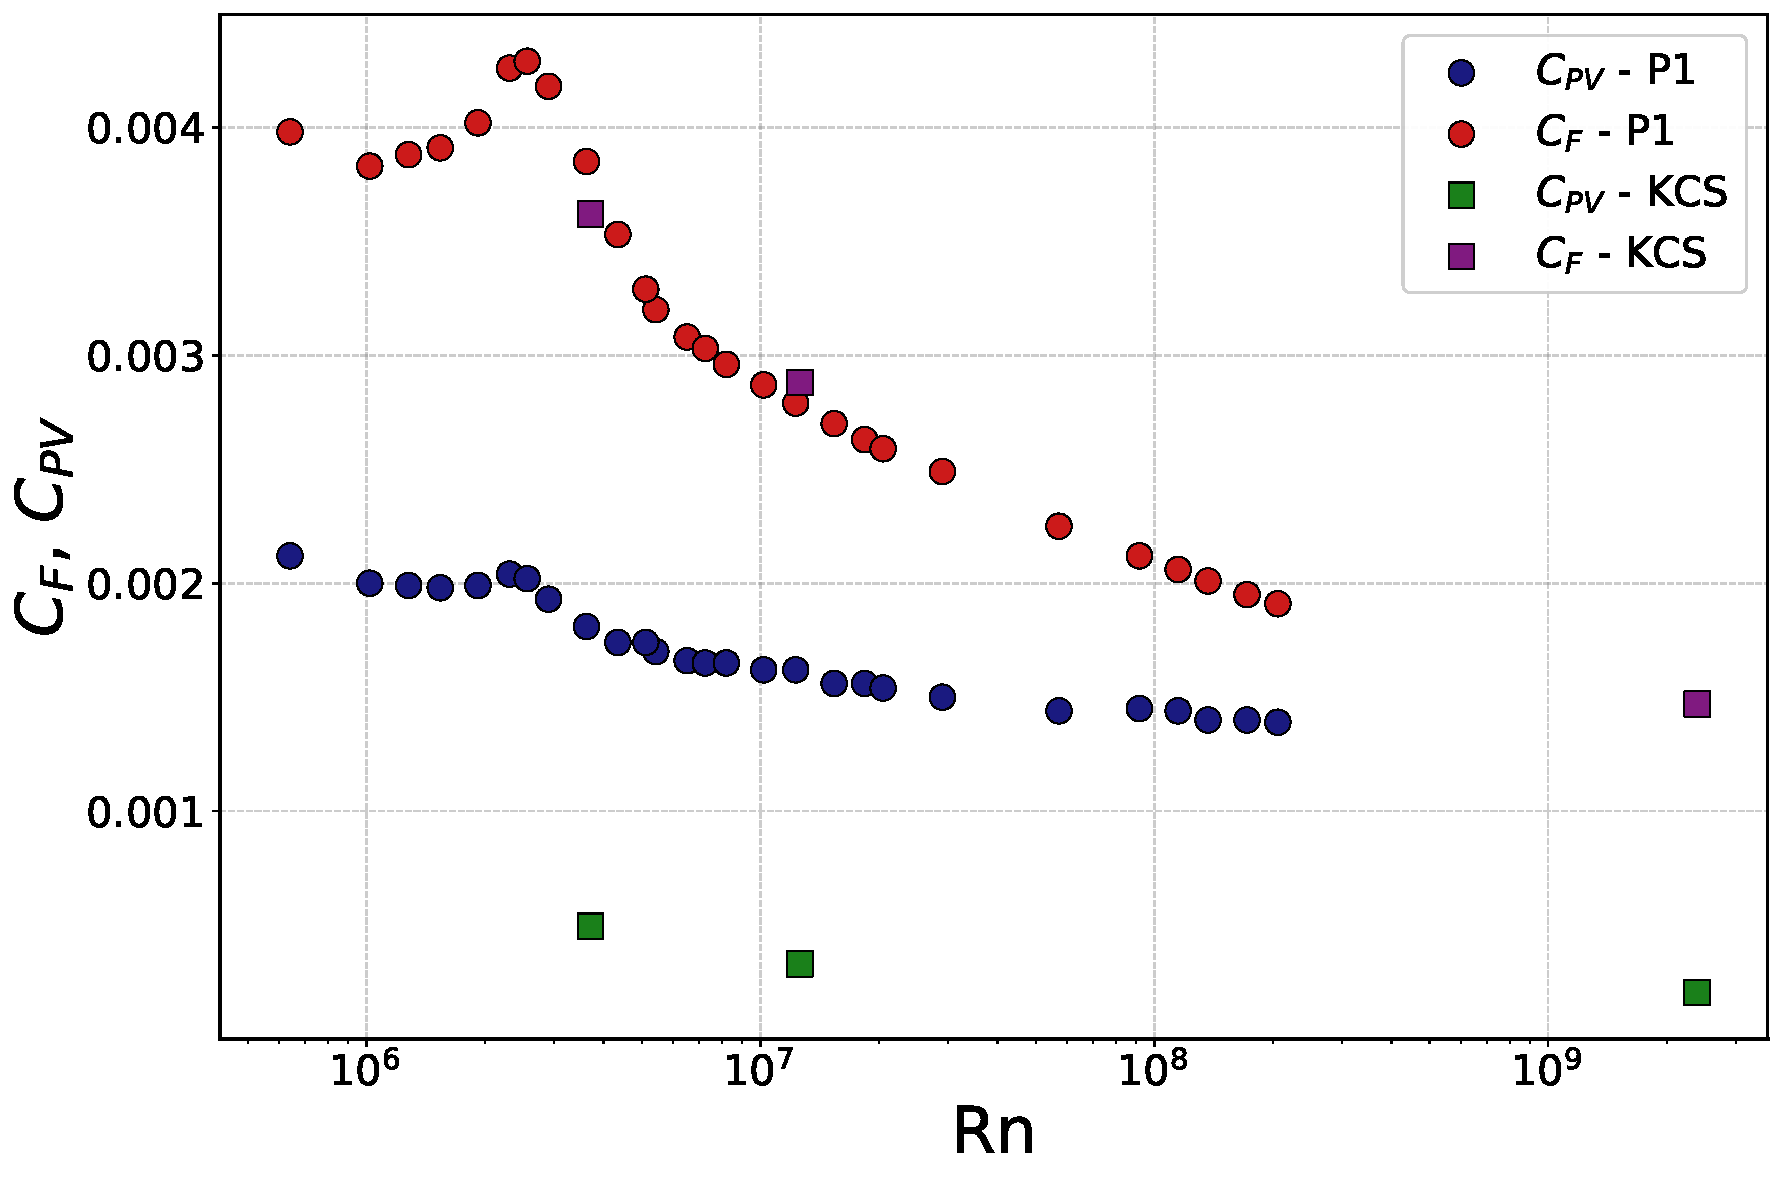
\includegraphics[width=.6\columnwidth]{./images/kcs_tpa_descomposicion.pdf}
\caption{$C_{PV}$ y $C_F$ obtenidos mediante CFD en doble cuerpo para el 
\textit{P1} y para el KCS 1:79 (LabHiNO).}
\label{cpv_friccion}
\end{figure}

A diferencia de $C_F$, el coeficiente $C_{PV}$ es poco sensible a variaciones 
de $Re$ y resulta fuertemente influenciado por la geometría del casco. Para 
comprender esta dependencia con la forma del casco, es necesario considerar 
dos mecanismos que compiten en la formación de la resistencia por presión 
viscosa. El primero es la contribución de la capa límite tridimensional, que 
disminuye con $Re$ a medida que la capa límite se adelgaza y se reduce la 
disipación de energía cinética viscosa a lo largo del casco. El segundo es la 
contribución de estructuras vorticosas generadas en el casco, entre las que 
se incluyen tanto vórtices longitudinales desprendidos de la quilla y el 
pantoque como la posible recirculación asociada a la popa espejo, cuya 
intensidad puede aumentar o mantenerse aproximadamente estable con $Re$. La 
curva resultante de $C_{PV}(Re)$ surge de la superposición de estas dos 
tendencias opuestas (capa límite vs. estructuras vorticosas). 
Interpretaciones similares de doble mecanismo han sido reportadas por 
\citet{ZENG2019106434} y \citet{Raven2016}, y son consistentes con los 
estudios de escalado de popas mojadas de \citet{KORKMAZ2022112590}. El aporte 
relativo de cada una de estas fuentes de vorticidad se analiza en detalle en 
la Sección~\ref{sec:popa_sumergida}.

La Figura~\ref{U_x_U_0} presenta contornos de la velocidad longitudinal 
$U_x/U_0$ a $x/L=0.05$, inmediatamente detrás de la sección de popa, para 
escala modelo (1:20, $Re \approx 10^6$) y escala buque (1:1, $Re \approx 10^8$), donde se aprecia el adelgazamiento de la capa límite con $Re$, como cabría esperar del primer mecanismo. Por otro lado, la Figura~\ref{vortex} muestra iso-superficies de criterio Q que revelan el sistema de estructuras 
vorticosas presentes en la popa para ambas escalas. Dichas estructuras se 
mantienen con intensidad similar al aumentar $Re$, lo que indica que es la 
persistencia de este segundo mecanismo, y no el primero, la causa del alto 
valor de $C_{PV}$ y de su débil sensibilidad al número de Reynolds para el 
\textit{P1}. La pequeña disminución de $C_{PV}$ con $Re$ observada puede 
atribuirse al efecto superpuesto de la reducción de la capa límite.

\begin{figure}
\centering
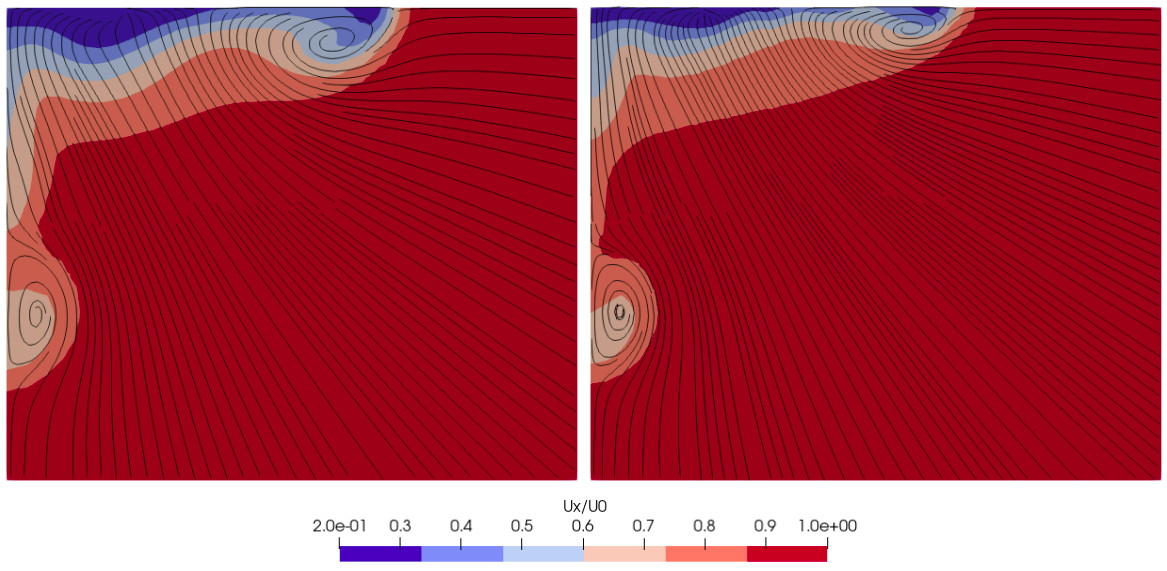
\includegraphics[width=1\columnwidth]{./images/U_x_U_0.png}
\caption{Contornos de velocidad longitudinal $U_x/U_0$ en un plano ubicado en 
$x/L=0.05$ para escala modelo, 1:20 (izquierda, $\log(Re) \approx 6$) y 
escala buque, 1:1 (derecha, $\log(Re) \approx 8$), a $Fr=0.2$.}
\label{U_x_U_0}
\end{figure}

\begin{figure}
\centering
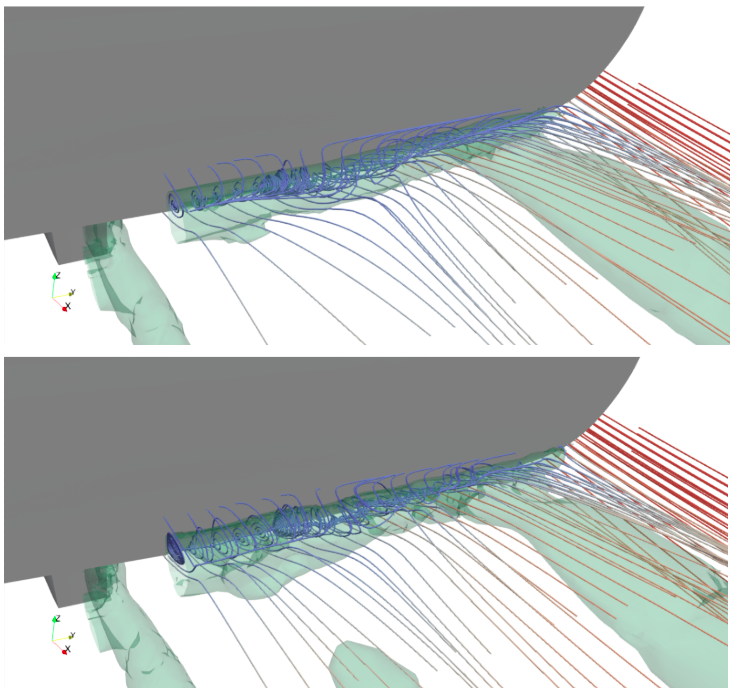
\includegraphics[width=.8\columnwidth]{./images/vortex.png}
\caption{Iso-superficies de Q-criterion (Q=10) mostrando las estructuras 
vorticosas presentes en la popa, a escala modelo, 1:20 (arriba, 
$\log(Re) \approx 6$) y escala buque, 1:1 (abajo, $\log(Re) \approx 8$), 
a $Fr=0.2$.}
\label{vortex}
\end{figure}

En síntesis, la descomposición presentada en esta sección permite explicar el 
comportamiento contrastante de $(1+k)$ entre ambos buques observado en la 
Sección~\ref{sec:analisis_efectos_escala}. En el KCS, la contribución de 
$C_{PV}$ al numerador de la Ecuación~\eqref{eq:descomposicion_1k} es 
comparativamente pequeña frente a $C_F$, de modo que $(1+k)$ queda dominado 
por el comportamiento de $C_F$, que sigue de cerca a $C_{F0}$ más allá de la 
región de transición y produce así un cociente prácticamente constante. En 
el \textit{P1}, en cambio, la magnitud comparable y la lenta caída de 
$C_{PV}$ frente a la caída más rápida de $C_{F0}$ impiden que el cociente se 
estabilice dentro del rango de escalas analizado. Este mecanismo, sostenido 
por la persistencia de estructuras vorticosas en la popa que no se atenúan 
significativamente con $Re$, es el responsable directo de la falta de valor 
asintótico de $(1+k)$ característica de este casco.

\subsubsection*{Taxonomía de mecanismos de efecto de escala}

Los resultados presentados permiten ubicar el comportamiento del
\textit{P1} dentro de un panorama más amplio de mecanismos por los cuales
el factor de forma puede depender de la escala. La literatura documenta al
menos tres mecanismos distintos, que se diferencian tanto por su origen
físico como por el signo de su efecto sobre $(1+k)$ al aumentar el número
de Reynolds.

El primero es la \textbf{separación tipo burbuja} en la popa de cascos de
formas llenas, originada por el gradiente de presión adverso que sigue a la
región de baja presión del pantoque. A medida que aumenta $Re$, la
influencia de la viscosidad disminuye, la separación se atenúa y la
contribución de la resistencia de forma respecto de la viscosa se reduce,
de modo que $(1+k)$ \textit{decrece} con la escala
\citep{korkmaz-verif-and-valid-cfd-efd}. El segundo es la
\textbf{recirculación tras un espejo de popa sustancialmente sumergido},
análoga al flujo sobre un escalón hacia atrás. A diferencia del anterior,
esta estructura persiste al aumentar $Re$ y genera un incremento acotado
del factor de forma entre modelo y buque, cuantificado mediante el
\textit{transom form factor} $k_{tr}>0$ \citep{korkmaz_wetted_transom}; su
aplicación al \textit{P1} se analiza en la
Sección~\ref{sec:popa_sumergida}.

El mecanismo dominante en el \textit{P1}, en cambio, es distinto de ambos y
responde a la geometría de baja esbeltez del casco: se trata de la
persistencia de \textbf{estructuras vorticosas longitudinales} desprendidas
de la quilla y el pantoque, cuya intensidad no se atenúa apreciablemente
con $Re$, según se documentó mediante los contornos de velocidad
(Figura~\ref{U_x_U_0}) y las iso-superficies de criterio Q
(Figura~\ref{vortex}). Este mecanismo sostiene un valor elevado y poco
sensible de $C_{PV}$, lo que hace que $(1+k)$ \textit{crezca} de manera
sostenida y sin alcanzar un valor asintótico dentro del rango de escalas
analizado. El contraste de signo respecto de la separación tipo burbuja es
significativo: mientras en aquel caso el aumento de $Re$ tiende a
\textit{recuperar} el comportamiento de placa plana, en los pesqueros de
baja esbeltez el efecto tridimensional persiste hasta la escala buque. Esta
diferencia es la que confiere carácter distintivo al resultado y la que
explica por qué las correcciones concebidas para los dos primeros
mecanismos resultan insuficientes para esta clase de cascos, como se
verifica en las Secciones~\ref{sec:popa_sumergida}
y~\ref{sec:linea_de_friccion}.

\subsection{Distribución de presiones sobre el casco}

En esta sección se analiza la distribución del coeficiente de presión 
($C_P$) sobre el casco del \textit{P1} para distintas escalas. Este 
parámetro se define como:

\begin{equation}
    C_{P} = \frac{p - p_\infty}{\tfrac{1}{2}\rho V^2},
\end{equation}

donde $p$ es la presión sobre el casco, $p_\infty$ la presión del flujo 
incidente sin perturbaciones, $V$ la velocidad del buque y $\rho$ la densidad 
del agua. El coeficiente $C_{PV}$ surge de integrar $C_P$ sobre la superficie 
mojada y proyectarlo en la dirección de avance, por lo que el estudio 
detallado de su distribución permite comprender mejor la evolución de 
$C_{PV}$ con el número de Reynolds.

Las Figuras~\ref{cp_bow}, \ref{cp_stern}, \ref{cp_bottom} y \ref{cp_side} 
muestran la distribución de $C_P$ sobre el casco del \textit{P1} para escala 
modelo (1:20) y escala buque (1:1), a $Fr=0.2$, vistas desde la proa, la 
popa, el fondo y el costado respectivamente.

\begin{figure}
\centering
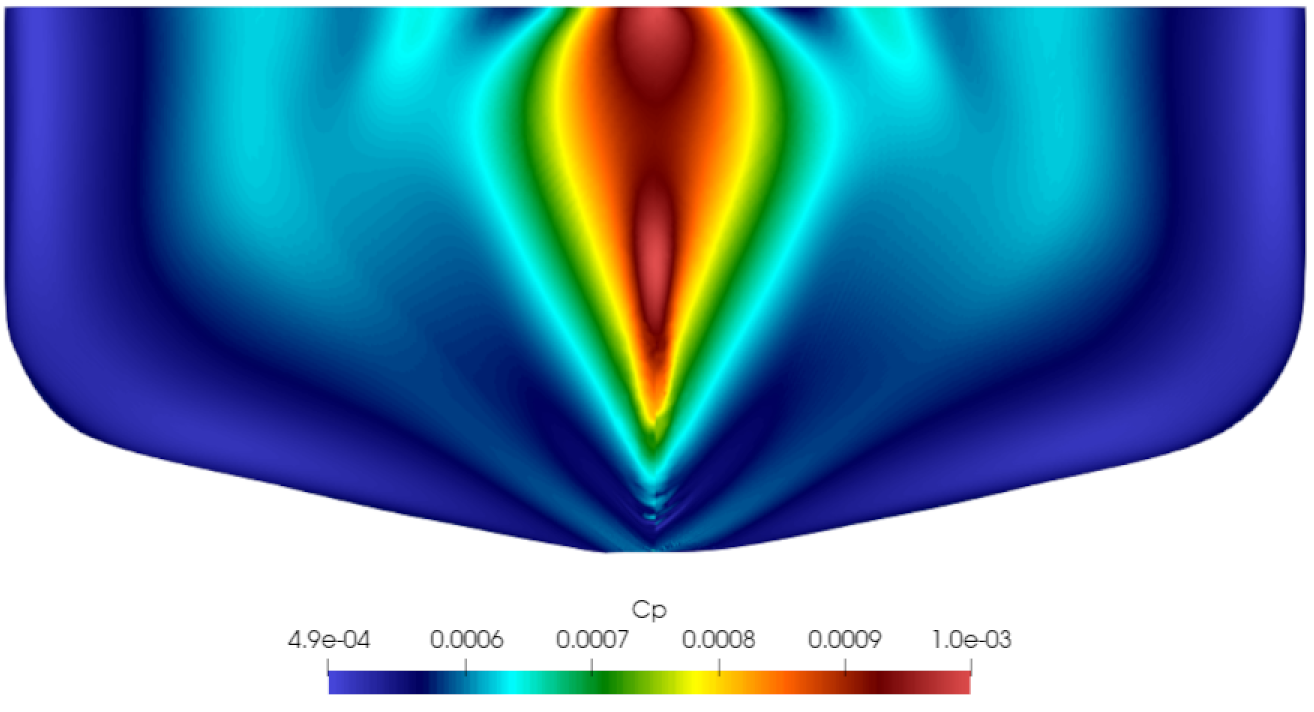
\includegraphics[width=.6\columnwidth]{./images/cp_proa2.png}
\caption{$C_P$ para $Fr=0.2$, vista de proa. Izquierda: escala 1:20. 
Derecha: escala 1:1.}
\label{cp_bow}
\end{figure}

\begin{figure}
\centering
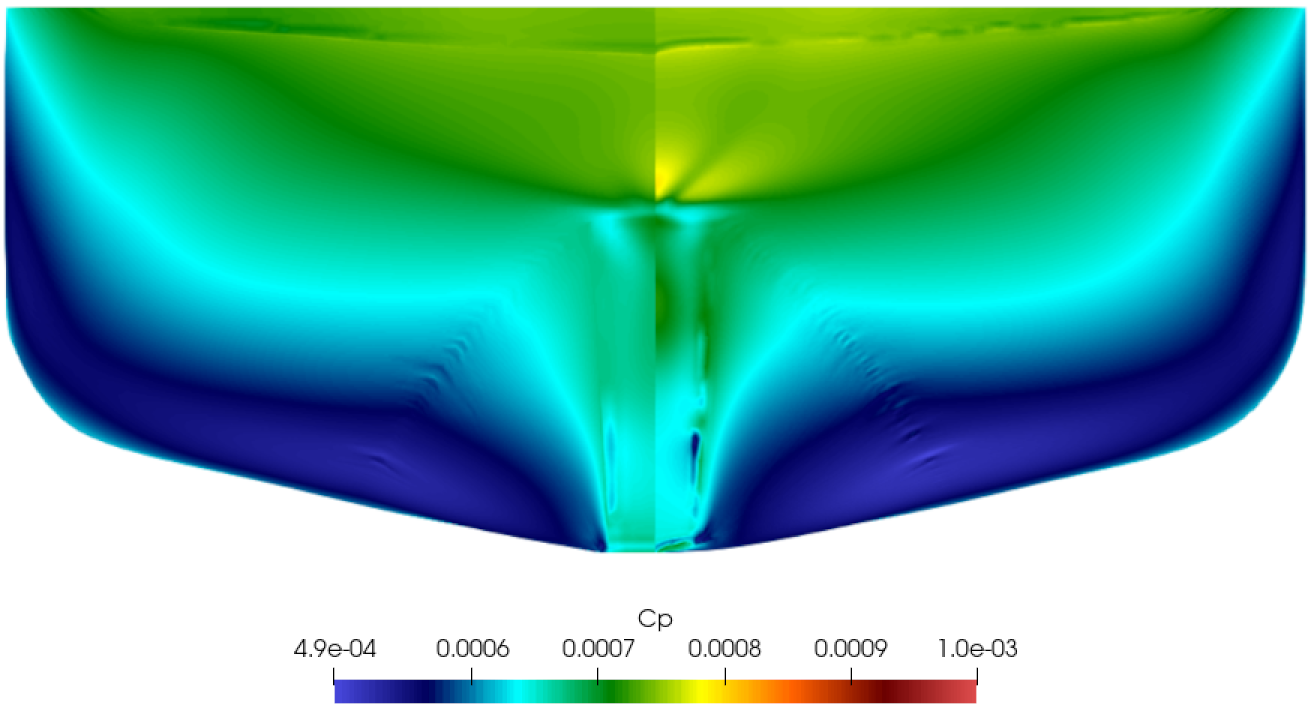
\includegraphics[width=.6\columnwidth]{./images/cp_popa2.png}
\caption{$C_P$ para $Fr=0.2$, vista de popa. Izquierda: escala 1:20. 
Derecha: escala 1:1.}
\label{cp_stern}
\end{figure}

\begin{figure}
\centering
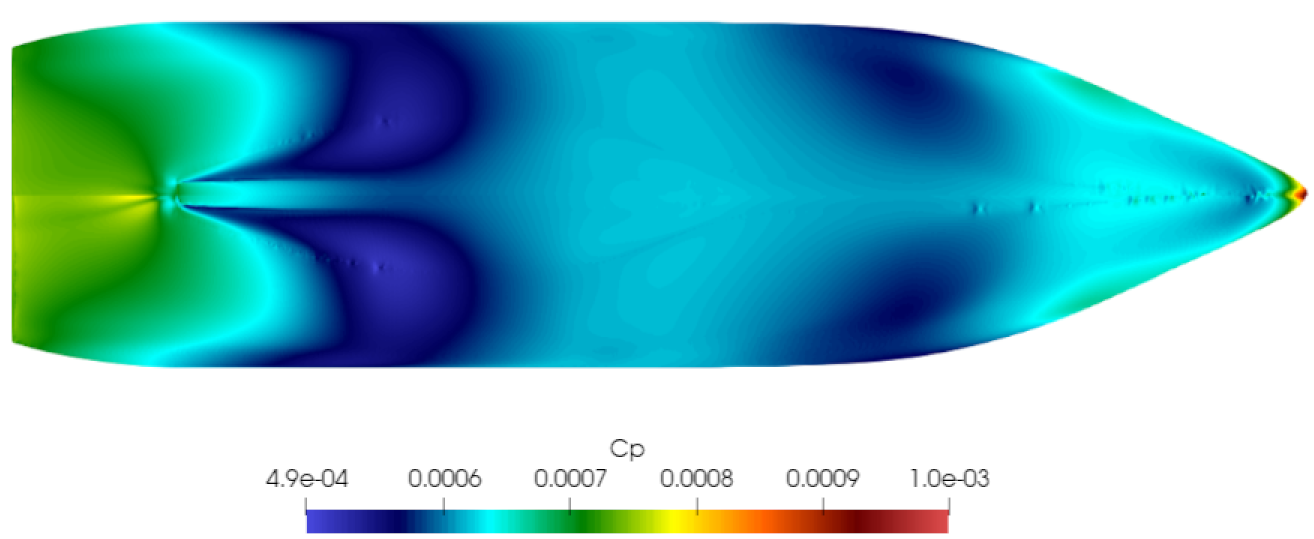
\includegraphics[width=.6\columnwidth]{./images/cp_fondo2.png}
\caption{$C_P$ para $Fr=0.2$, vista desde el fondo. Arriba: escala 1:20. 
Abajo: escala 1:1.}
\label{cp_bottom}
\end{figure}

\begin{figure}
\centering
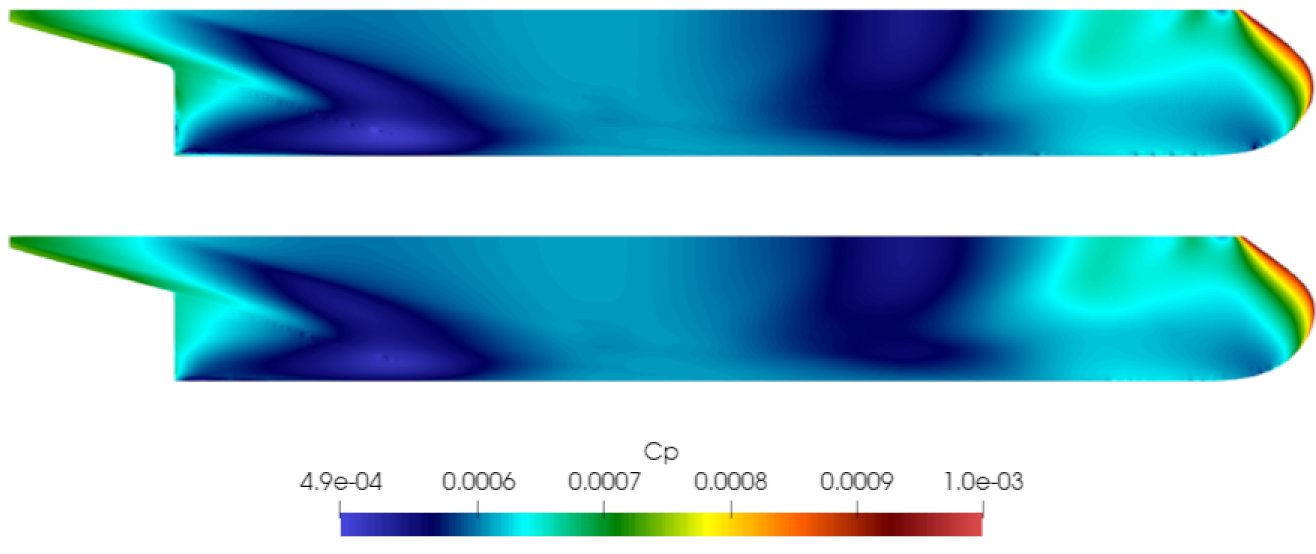
\includegraphics[width=.6\columnwidth]{./images/cp_lateral2.png}
\caption{$C_P$ para $Fr=0.2$, vista lateral. Arriba: escala 1:20. Abajo: 
escala 1:1.}
\label{cp_side}
\end{figure}

Los resultados indican que la recuperación de presión en la zona de popa es 
considerablemente menor que en cascos más hidrodinámicos, como el KCS 
\citep{cp_recovery_kcs}, lo cual explica los altos valores de $(1+k)$ 
observados en este tipo de buques. En cuanto al efecto del número de 
Reynolds sobre $C_P$, se observa una diferencia muy leve en la distribución 
de presiones en la zona de popa entre escalas: la presión en escala 1:1 
recupera ligeramente más que en escala 1:20, lo cual es consistente con la 
disminución muy leve de $C_{PV}$ con $Re$ observada para este buque.

Las Figuras~\ref{fig:cp_z0}, \ref{fig:cp_z5} y \ref{fig:cp_z75} presentan la 
distribución longitudinal del coeficiente de presión $C_{P}(x/L)$ para 
distintos números de Reynolds, sobre tres planos horizontales a profundidad 
constante $z/T = 0$, $0.5$ y $0.75$ respectivamente, es decir, en la línea de 
flotación, a media manga sumergida y cerca del fondo. La coordenada 
longitudinal se expresa como $x/L$, donde $x/L = 0$ corresponde a la 
perpendicular de proa. Se observa un déficit persistente de presión en la 
región de popa para todos los $Re$, en las tres líneas de agua analizadas, 
con variaciones mínimas entre escalas. La diferencia entre el caso a escala 
modelo ($Re=1.3\times10^6$) y el de escala buque ($Re=1.1\times10^8$) es del 
orden de $\Delta C_P = 0.01$--$0.02$, lo que indica que la recuperación de 
presión en popa es extremadamente débil y poco sensible a los efectos 
inerciales del flujo. Estos resultados cuantitativos son plenamente 
consistentes con la lenta disminución de $C_{PV}$ con el número de Reynolds, 
respaldando la conclusión de que las pérdidas por presión viscosa en la 
región de popa dominan el comportamiento del factor de forma $(1+k)$ para 
este casco.

\begin{figure}[htpb]
    \centering
    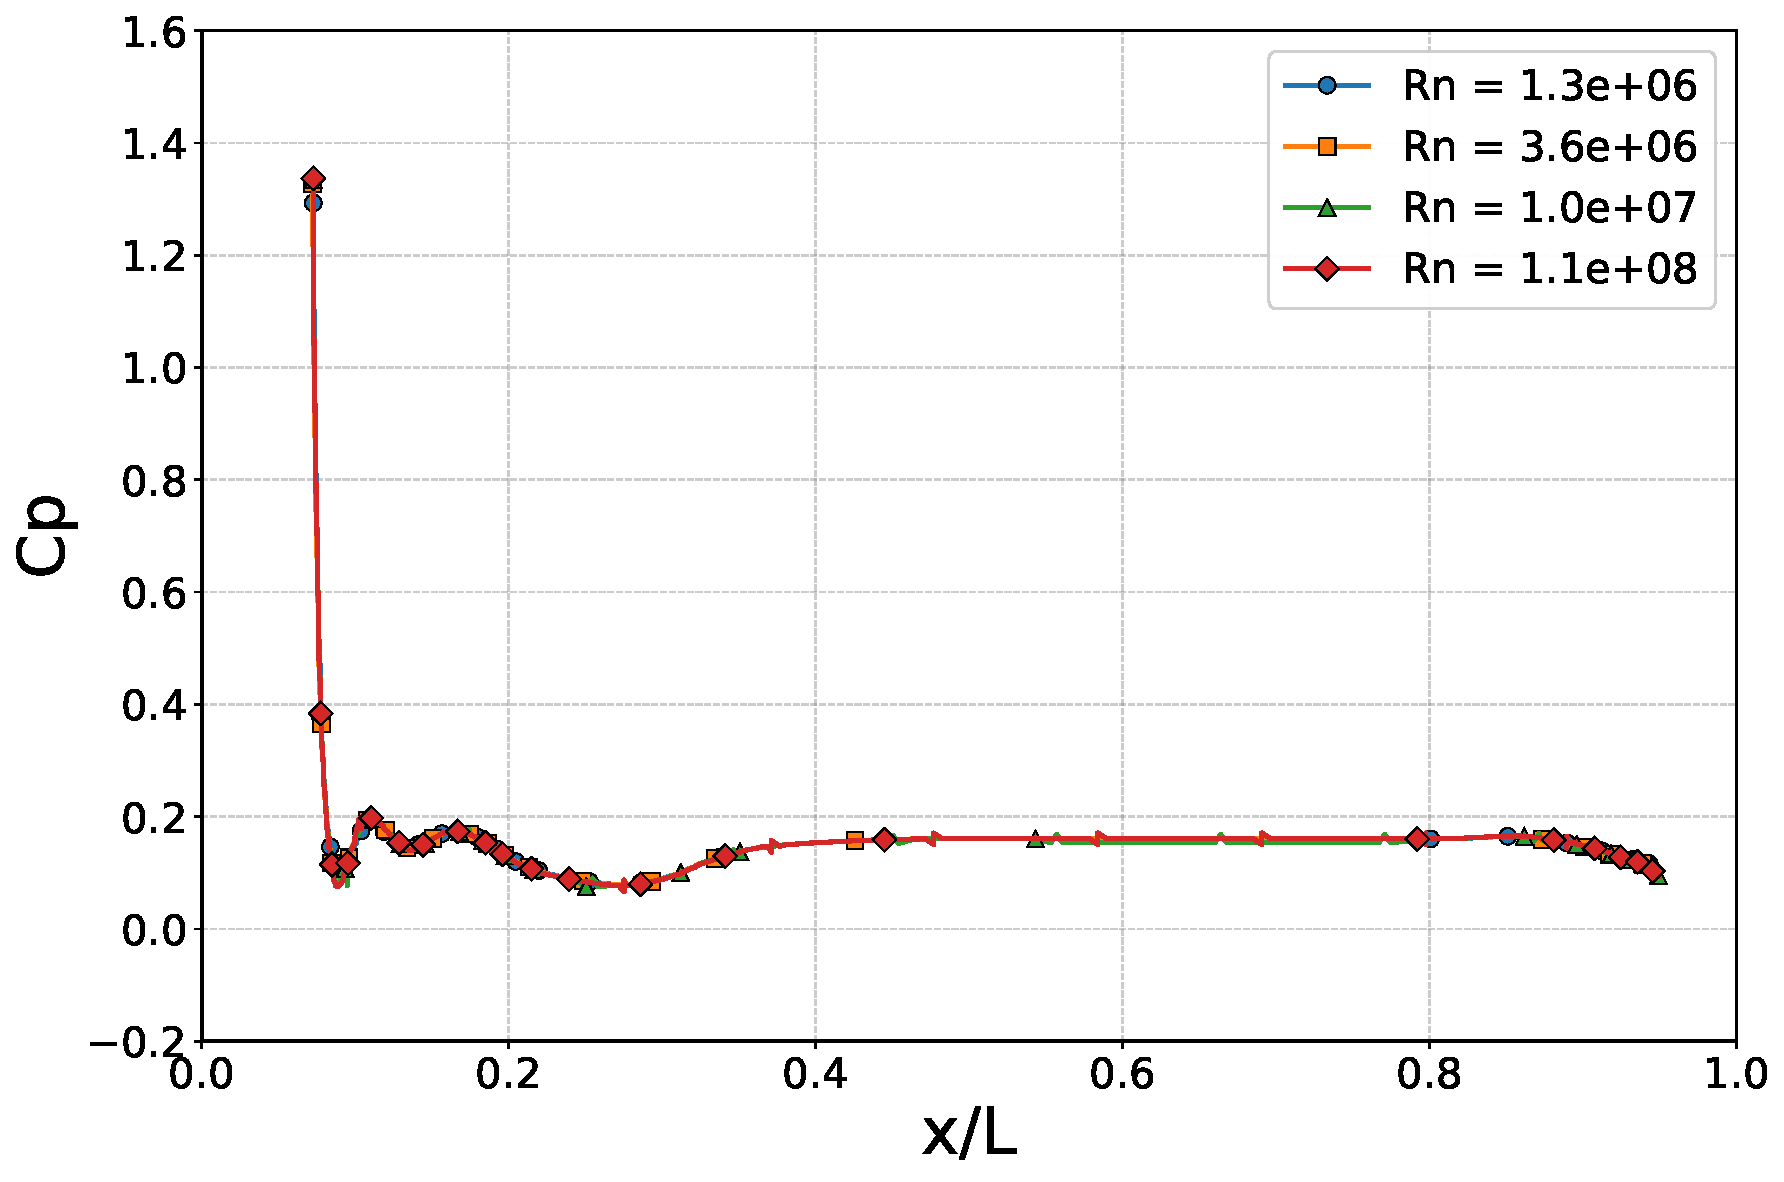
\includegraphics[width=.6\columnwidth]{./images/z0.pdf}
    \caption{Distribución de $C_{P}(x/L)$ sobre el plano $z/T = 0$ 
    (línea de flotación). Se observa un déficit persistente de presión 
    en popa y variaciones mínimas entre escalas.}
    \label{fig:cp_z0}
\end{figure}

\begin{figure}[htpb]
    \centering
    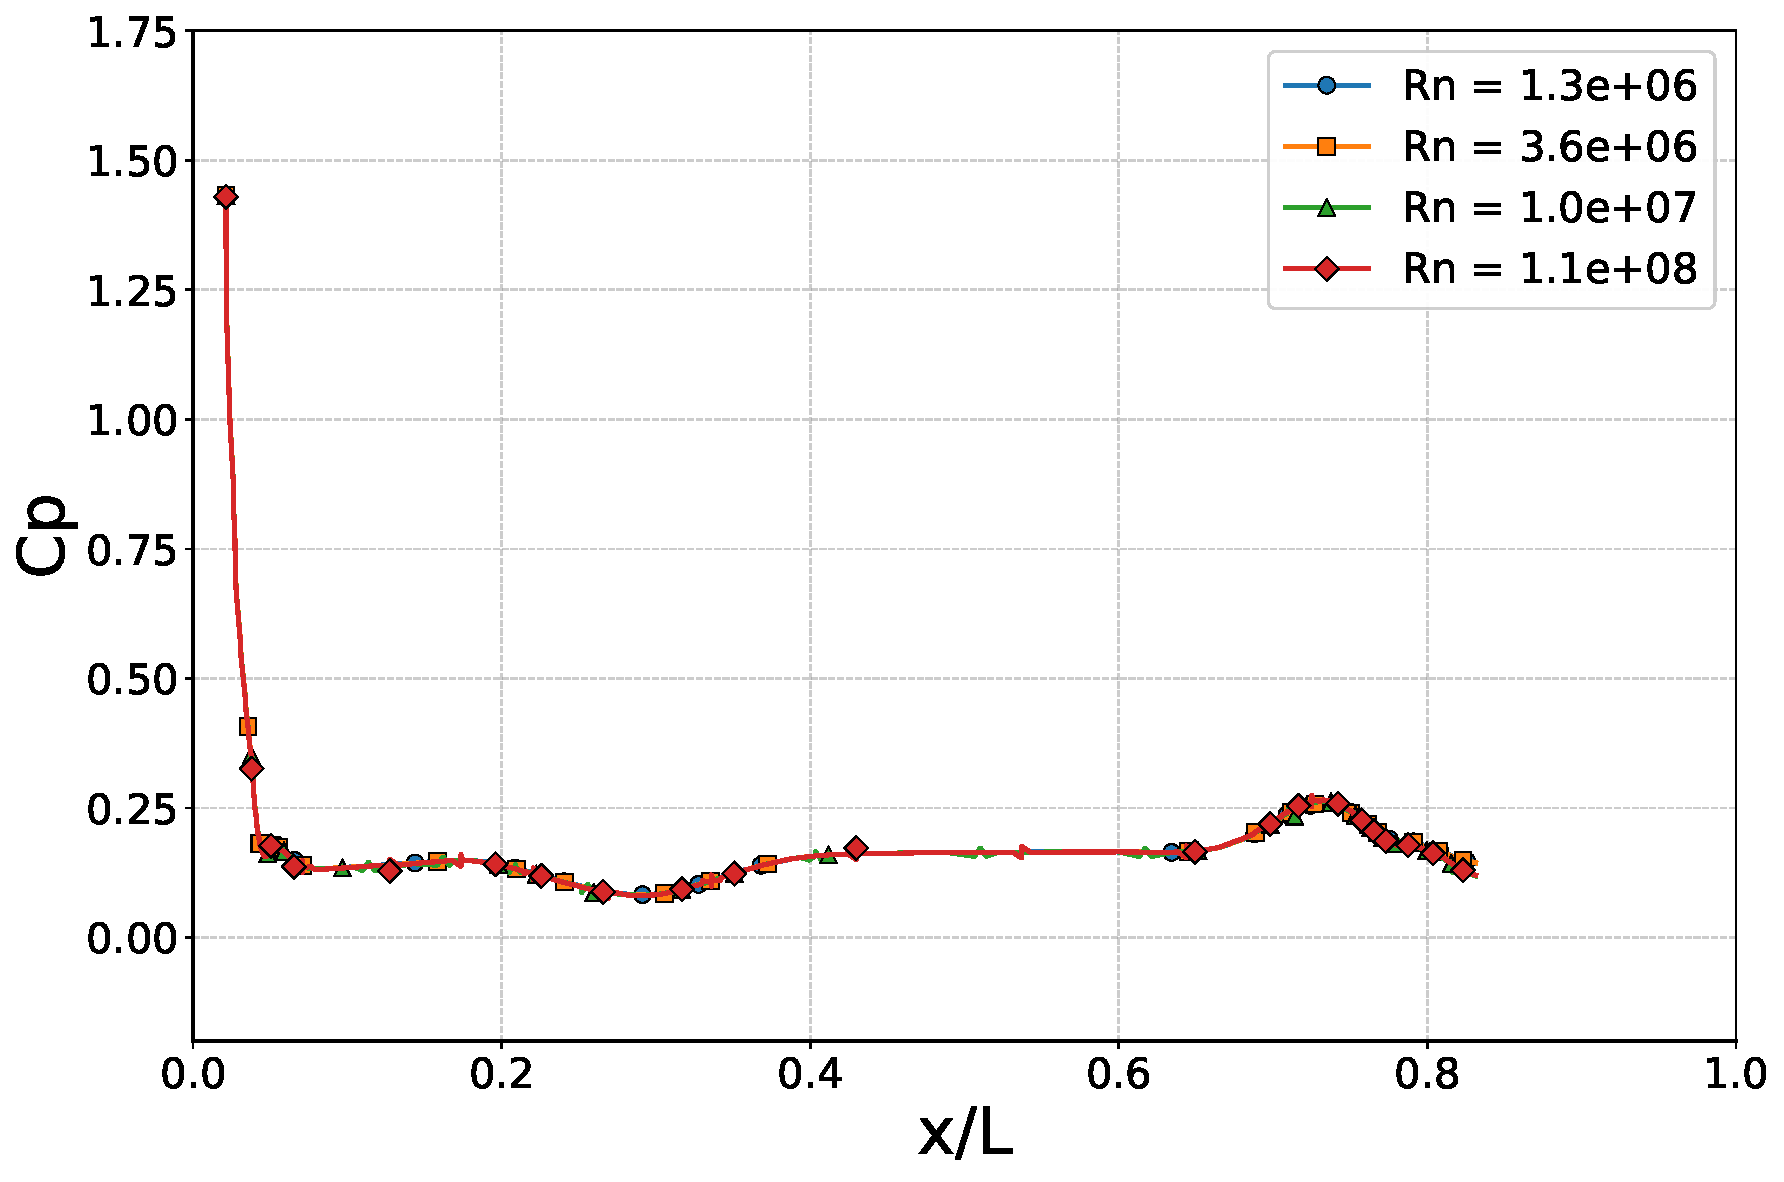
\includegraphics[width=.6\columnwidth]{./images/z5.pdf}
    \caption{Distribución de $C_{P}(x/L)$ sobre el plano $z/T = 0.5$.}
    \label{fig:cp_z5}
\end{figure}

\begin{figure}[htpb]
    \centering
    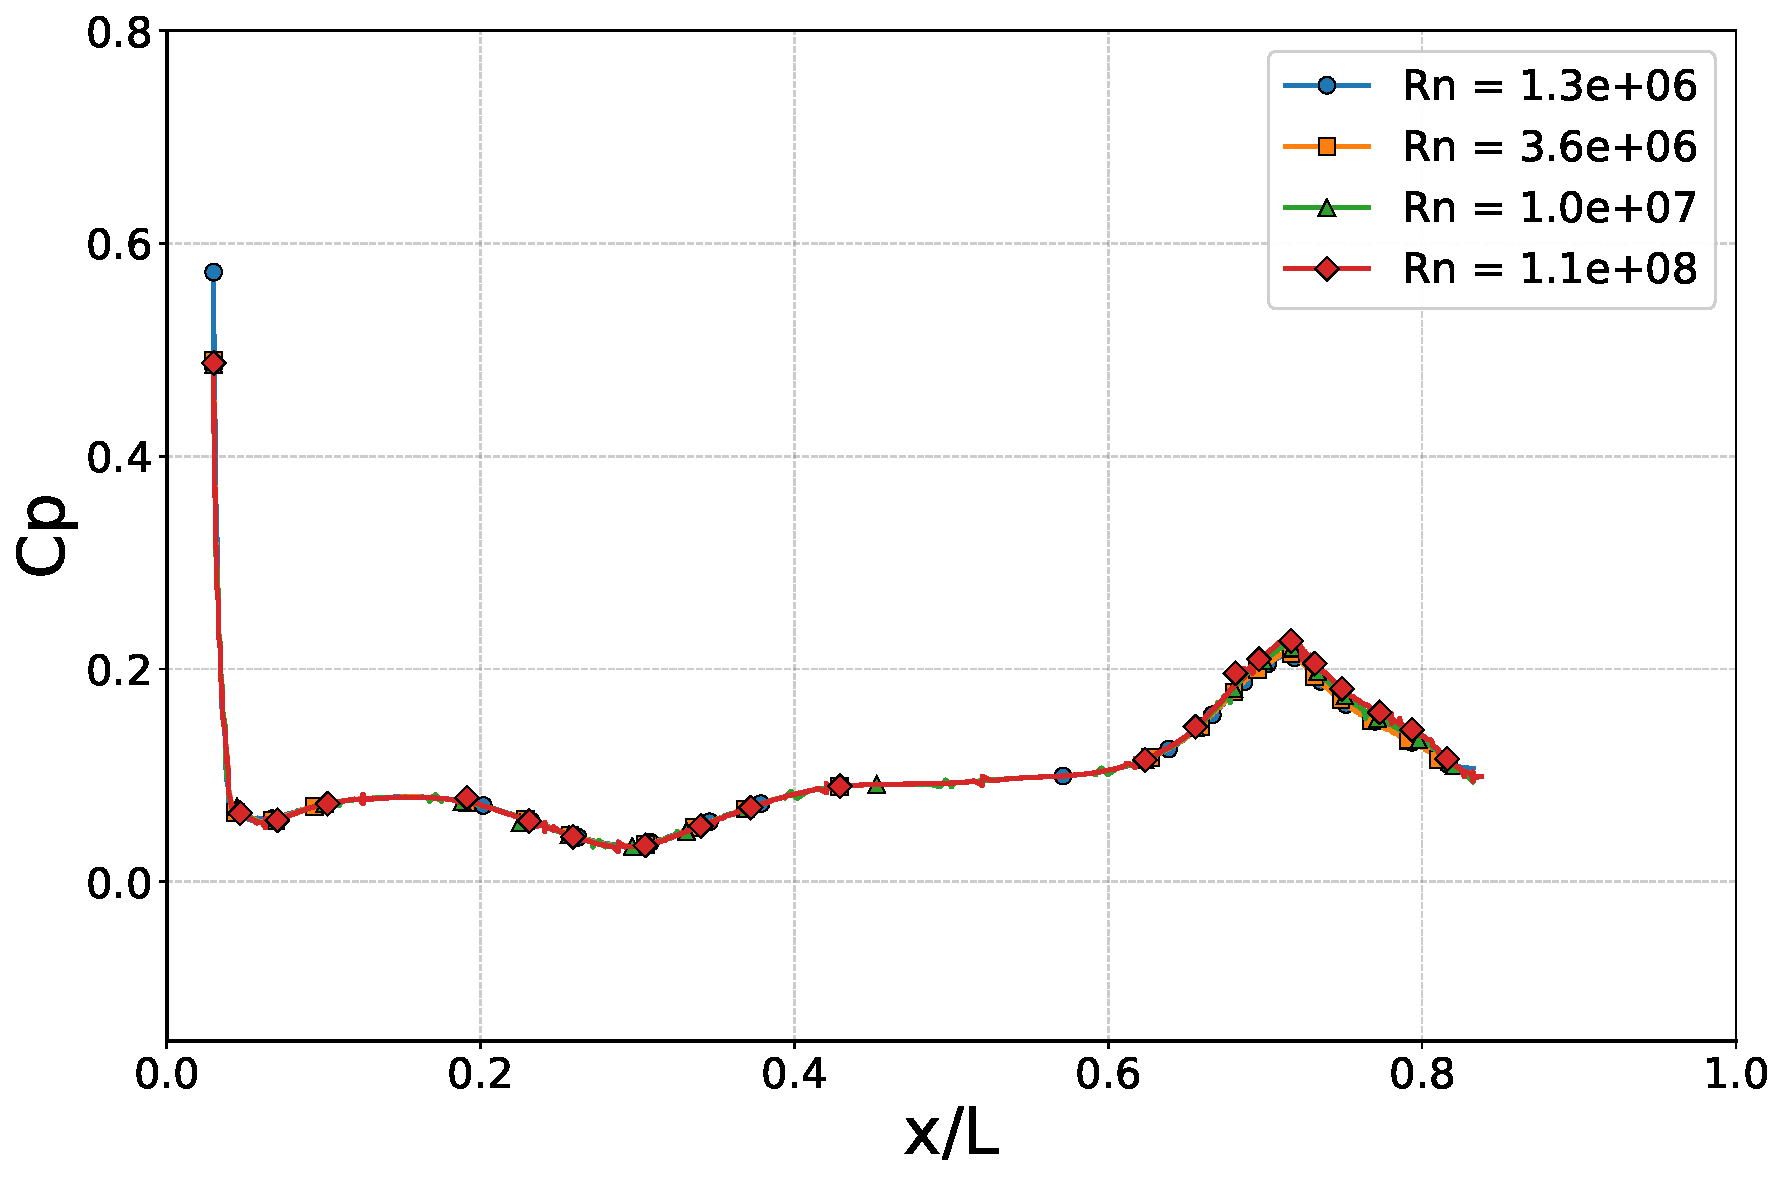
\includegraphics[width=.6\columnwidth]{./images/z75.pdf}
    \caption{Distribución de $C_{P}(x/L)$ sobre el plano $z/T = 0.75$.}
    \label{fig:cp_z75}
\end{figure}


\subsection{Conclusiones parciales}

El análisis de la distribución del coeficiente de presión $C_P$ confirma que 
el comportamiento del término de presión viscosa $C_{PV}$ está dominado por 
la región de popa del \textit{P1}. En todas las escalas analizadas se 
observa una recuperación de presión muy limitada en el cuerpo de salida, lo 
que conduce a pérdidas viscosas significativas asociadas a gradientes de 
presión adversos y a la persistencia de estructuras vorticosas de gran 
escala.

La comparación entre escala modelo y escala buque muestra que el efecto del 
número de Reynolds sobre la distribución de presiones es reducido. Si bien a 
escala buque se aprecia una recuperación de presión levemente mayor, las 
diferencias cuantitativas son pequeñas y se traducen únicamente en una 
disminución muy moderada de $C_{PV}$. Como se discutió en la 
Sección~\ref{sec:descomposicion_de_la_res_viscosa}, esta leve disminución 
puede atribuirse al efecto del adelgazamiento de la capa límite tridimensional con $Re$, mientras que la persistencia de las estructuras vorticosas de popa, prácticamente estables con la escala, explica que dicha disminución sea tan moderada. Este resultado explica la débil dependencia de la presión viscosa con $Re$ observada previamente y, en consecuencia, el crecimiento sostenido del factor de forma $(1+k)$ con la escala.

El déficit persistente de presión en popa, prácticamente invariante con el 
número de Reynolds, constituye así el mecanismo físico principal que 
distingue a los cascos de baja esbeltez de los cascos esbeltos convencionales. 
En este tipo de geometrías, las pérdidas por presión viscosa dominan la 
resistencia viscosa total y limitan la validez de los supuestos clásicos de 
extrapolación, reforzando la necesidad de considerar explícitamente los 
efectos geométricos en la estimación del factor de forma.

\section{Influencia de la proa bulbo en el factor de forma}\label{sec:proa_bulbo}

\subsection{Motivación y antecedentes sobre proa bulbo en pesqueros}

La incorporación de una proa bulbo en cascos pesqueros suele tener dos 
objetivos. Por un lado, aumentar el desplazamiento del casco, siendo esta 
una de las únicas variables disponibles dadas las limitaciones de eslora 
establecidas por las reglamentaciones nacionales. Por otro lado, busca 
reducir la resistencia por formación de olas en el rango de velocidades de 
servicio, mediante la generación de un sistema de ondas que interfiera 
destructivamente con el tren de olas producido por el resto del casco.

Como se discutió en la Sección~\ref{sec:prohaska_antec}, 
\citet{korkmaz_cfd_2021} reportaron que la geometría de la proa bulbo puede 
tener un impacto significativo en la aplicabilidad del método de Prohaska, 
llegando a introducir curvaturas marcadas en el diagrama que obligan a 
restringir severamente el rango de $Fr$ analizado, o incluso a descartar el 
método. El efecto se atribuye a la proximidad del bulbo a la superficie 
libre, que genera un sistema de ondas propio cuya interacción con el tren de 
proa no responde a la ley $Fr^4$ supuesta por el método.

El \textit{P1} presenta ambas anomalías: la curvatura cóncava a bajos 
números de Froude en su diagrama de Prohaska 
(Sección~\ref{sec:det_num_fac_form}) y la ausencia de un valor asintótico de 
$(1+k)$ con la velocidad y con la escala 
(Sección~\ref{sec:analisis_efectos_escala}), en contraste con el 
comportamiento del KCS. Ambas observaciones motivan la pregunta de 
investigación que organiza esta sección: \textit{¿es la proa bulbo 
responsable, total o parcialmente, de dichas anomalías?} Para responderla se 
repite el procedimiento completo de determinación del factor de forma sobre 
una variante del casco sin bulbo, de modo que cualquier comportamiento que 
persista en esa configuración no pueda atribuirse a su presencia.

\subsection{Modelos numéricos}

Para aislar el efecto del bulbo se generó un modelo modificado del 
\textit{P1} a escala 1:20, denominado ``Ctrl+Z'' en alusión al comando de 
deshacer, en referencia a que revierte la tendencia actual de incorporar 
proas bulbo en el diseño de pesqueros. El criterio de modificación consistió 
en eliminar el bulbo del modelo original manteniendo sin cambios el resto de 
la geometría del casco, de modo que ambos modelos resulten comparables y la 
única diferencia entre ellos sea la presencia o ausencia del bulbo. Este 
análisis se realizó exclusivamente a escala modelo, en una etapa temprana de 
la investigación, previa a la extensión del estudio a escalas mayores 
presentada en la Sección~\ref{sec:analisis_efectos_escala}.

Dado que el bulbo se encuentra completamente sumergido, su eliminación no 
modifica la eslora de flotación, que permanece idéntica en ambas 
configuraciones y define por lo tanto un mismo número de Froude para una 
misma velocidad. Sí se modifica, en cambio, la eslora mojada, que se reduce 
de $1{.}634$ a $1{.}515$~m para $T = 0{.}165$~m y de $1{.}641$ a $1{.}575$~m 
para $T = 0{.}195$~m. Esta distinción es relevante porque es la eslora 
mojada la que interviene en el número de Reynolds y, en consecuencia, en el 
coeficiente de fricción de referencia $C_{F0}$ empleado para la 
descomposición: a igual velocidad, la configuración con bulbo opera a un 
$Re$ mayor y por lo tanto a un $C_{F0}$ menor. Todas las comparaciones 
presentadas a continuación se realizan a igual número de Froude, es decir, a 
igual velocidad, empleando para cada configuración su propia eslora mojada 
en el cálculo de $Re$.

La Figura~\ref{fig:tpa_y_ctrlZ} presenta, para ambos modelos, la vista de 
perfil con la curva de áreas superpuesta (en rojo) y la vista en perspectiva 
del casco. La curva de áreas representa el área de la sección transversal 
sumergida en función de la posición longitudinal, y permite visualizar de 
manera directa cómo se modifica la distribución de volumen del casco al 
eliminar el bulbo: en el modelo original (Figura~\ref{fig:tpa_y_ctrlZ}a) se 
observa el incremento de área característico en la zona de proa asociado al 
bulbo, mientras que en el modelo Ctrl+Z (Figura~\ref{fig:tpa_y_ctrlZ}b) dicha 
protuberancia desaparece, conservándose el resto de la distribución de 
volumen prácticamente sin cambios.

\begin{figure}
    \centering
    \begin{subfigure}{\linewidth}
        \centering
        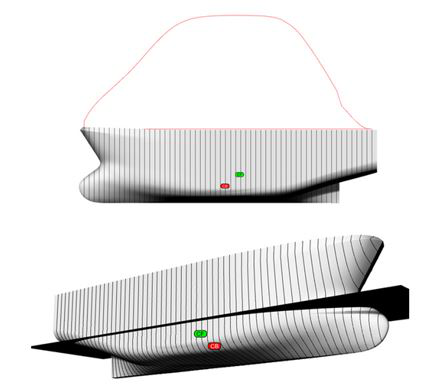
\includegraphics[width=.6\columnwidth]{./images/A1.png}
        \caption{Modelo original.}
    \end{subfigure}

    \vspace{1em}

    \begin{subfigure}{\linewidth}
        \centering
        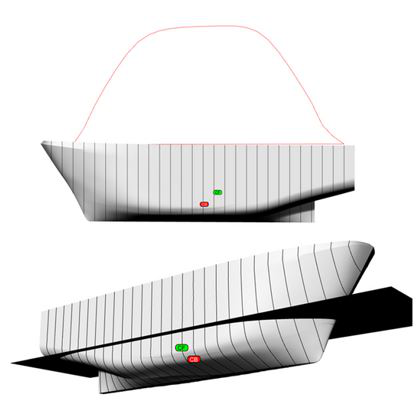
\includegraphics[width=.6\columnwidth]{./images/A2.png}
        \caption{Modelo Ctrl+Z.}
    \end{subfigure}

    \caption{Comparación entre el modelo original del \textit{P1} y el 
    modelo Ctrl+Z, sin proa bulbo, junto con sus curvas de áreas 
    correspondientes (en rojo).}
    \label{fig:tpa_y_ctrlZ}
\end{figure}


\subsection{Resultados de resistencia para diferentes configuraciones de proa 
en todo el rango de operación}

Para evaluar el impacto de la proa bulbo sobre la resistencia del 
\textit{P1}, se compararon las curvas de resistencia total ($C_T$), viscosa 
($C_V$) y por olas ($C_W$) en función del número de Froude, para los dos 
modelos (con y sin bulbo) y los dos calados disponibles ($T = 0{.}165$~m y 
$T = 0{.}195$~m). El coeficiente $C_T$ se obtuvo directamente de las 
simulaciones bifásicas con superficie libre para cada configuración. El 
coeficiente $C_V$ se calculó como:
%
\begin{equation}
    C_V = (1+k)\, C_{F0}
\end{equation}
%
empleando, para cada configuración, el factor de forma $k$ determinado 
mediante el método de Prohaska a partir de sus propias simulaciones CFD 
bifásicas: para el modelo original con bulbo, el valor validado contra el 
ensayo experimental (Sección~\ref{sec:det_exp_fac_form}); para el modelo 
Ctrl+Z, el valor obtenido aplicando el mismo procedimiento a sus 
simulaciones, sin contar con un ensayo experimental propio de validación. 
Finalmente, el coeficiente de resistencia por olas se obtuvo como residuo:
%
\begin{equation}
    C_W = C_T - C_V
\end{equation}

Los diagramas de Prohaska correspondientes a ambas configuraciones se 
presentan en las Figuras~\ref{fig:prohaska_bulbo_165} y 
\ref{fig:prohaska_bulbo_195}. En ambos calados se observa que la curvatura 
cóncava a bajos números de Froude, ya identificada para el modelo original 
en la Sección~\ref{sec:det_num_fac_form}, se reproduce con igual intensidad 
en la configuración Ctrl+Z. Este resultado permite descartar la primera de 
las hipótesis planteadas: la deformación del diagrama de Prohaska no 
responde a la presencia del bulbo, sino que constituye una característica 
propia del resto del casco. La anomalía reportada por 
\citet{korkmaz_cfd_2021} para cascos con bulbo próximo a la superficie libre 
no explica, por lo tanto, el comportamiento observado en el \textit{P1}.

Descartada la proa bulbo, subsisten dos de las causas enumeradas en la 
Sección~\ref{sec:prohaska_antec}: la geometría del resto del casco y el 
modelado numérico de la zona de transición. Ambas configuraciones fueron 
simuladas con el mismo cierre turbulento ($k$--$\omega$ SST) y operan en el 
mismo rango de números de Reynolds, de modo que la comparación entre ellas 
no permite discriminar entre ambos orígenes: el adelantamiento del punto de 
transición que introduce un modelo formulado para régimen enteramente 
turbulento, discutido en la Sección~\ref{sec:det_num_fac_form}, afecta por 
igual a los dos casos y no puede aislarse eliminando el bulbo.

Existe, no obstante, un indicio a favor del origen numérico. Como se señaló 
en la Sección~\ref{sec:det_num_fac_form}, la desviación observada en los 
ensayos experimentales es convexa, mientras que la de las simulaciones es 
cóncava. Este cambio de signo sugiere que la concavidad no reproduce un 
fenómeno físico del casco sino que constituye un artefacto de la 
simulación, asociado a la incapacidad del modelo de turbulencia empleado 
para representar la fracción de capa límite que permanece laminar a los 
$Re$ de escala modelo. Dirimir definitivamente esta cuestión requeriría 
repetir las simulaciones con un modelo de transición del tipo 
$\gamma$--$\widetilde{Re}_{\theta t}$ (Sección~\ref{sec:modelos_transicion}), 
lo que excede el alcance de esta sección y queda planteado como línea de 
trabajo futuro.

\begin{figure}[htpb]
	\centering
	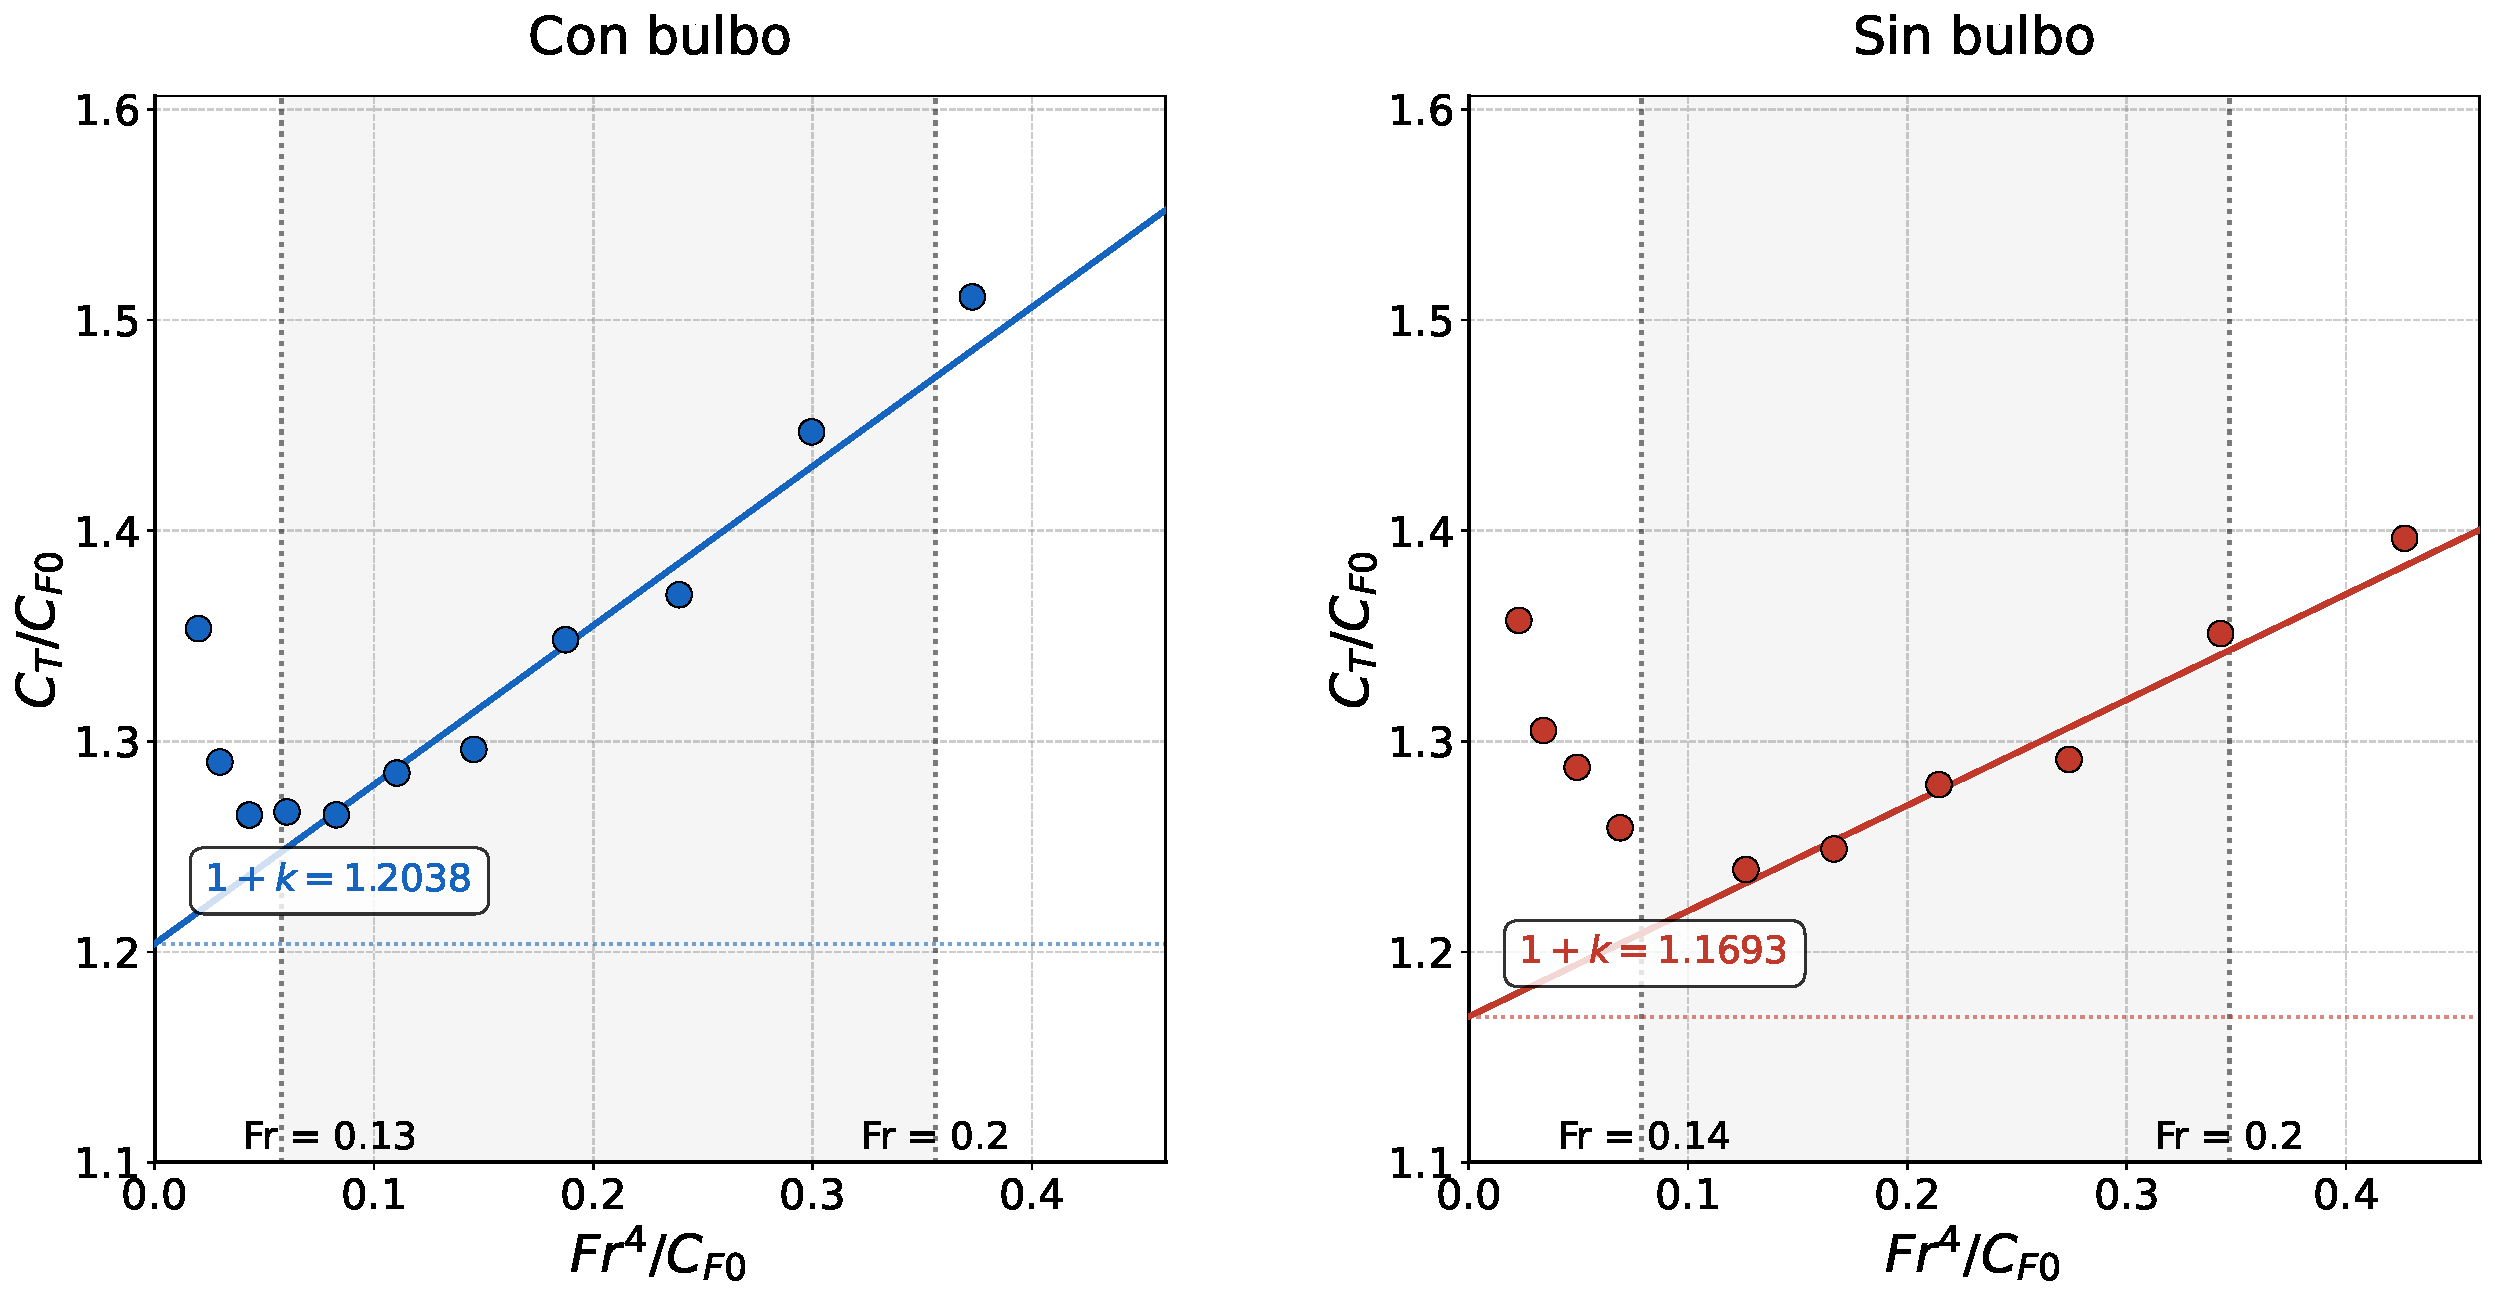
\includegraphics[width=.9\textwidth]{images/prohaska-bulbo-ctrlz-165.pdf}
	\caption{Diagrama de Prohaska comparando modelos con y sin bulbo 
	($T = 0{.}165$~m).}
	\label{fig:prohaska_bulbo_165}
\end{figure}

\begin{figure}[htpb]
	\centering
	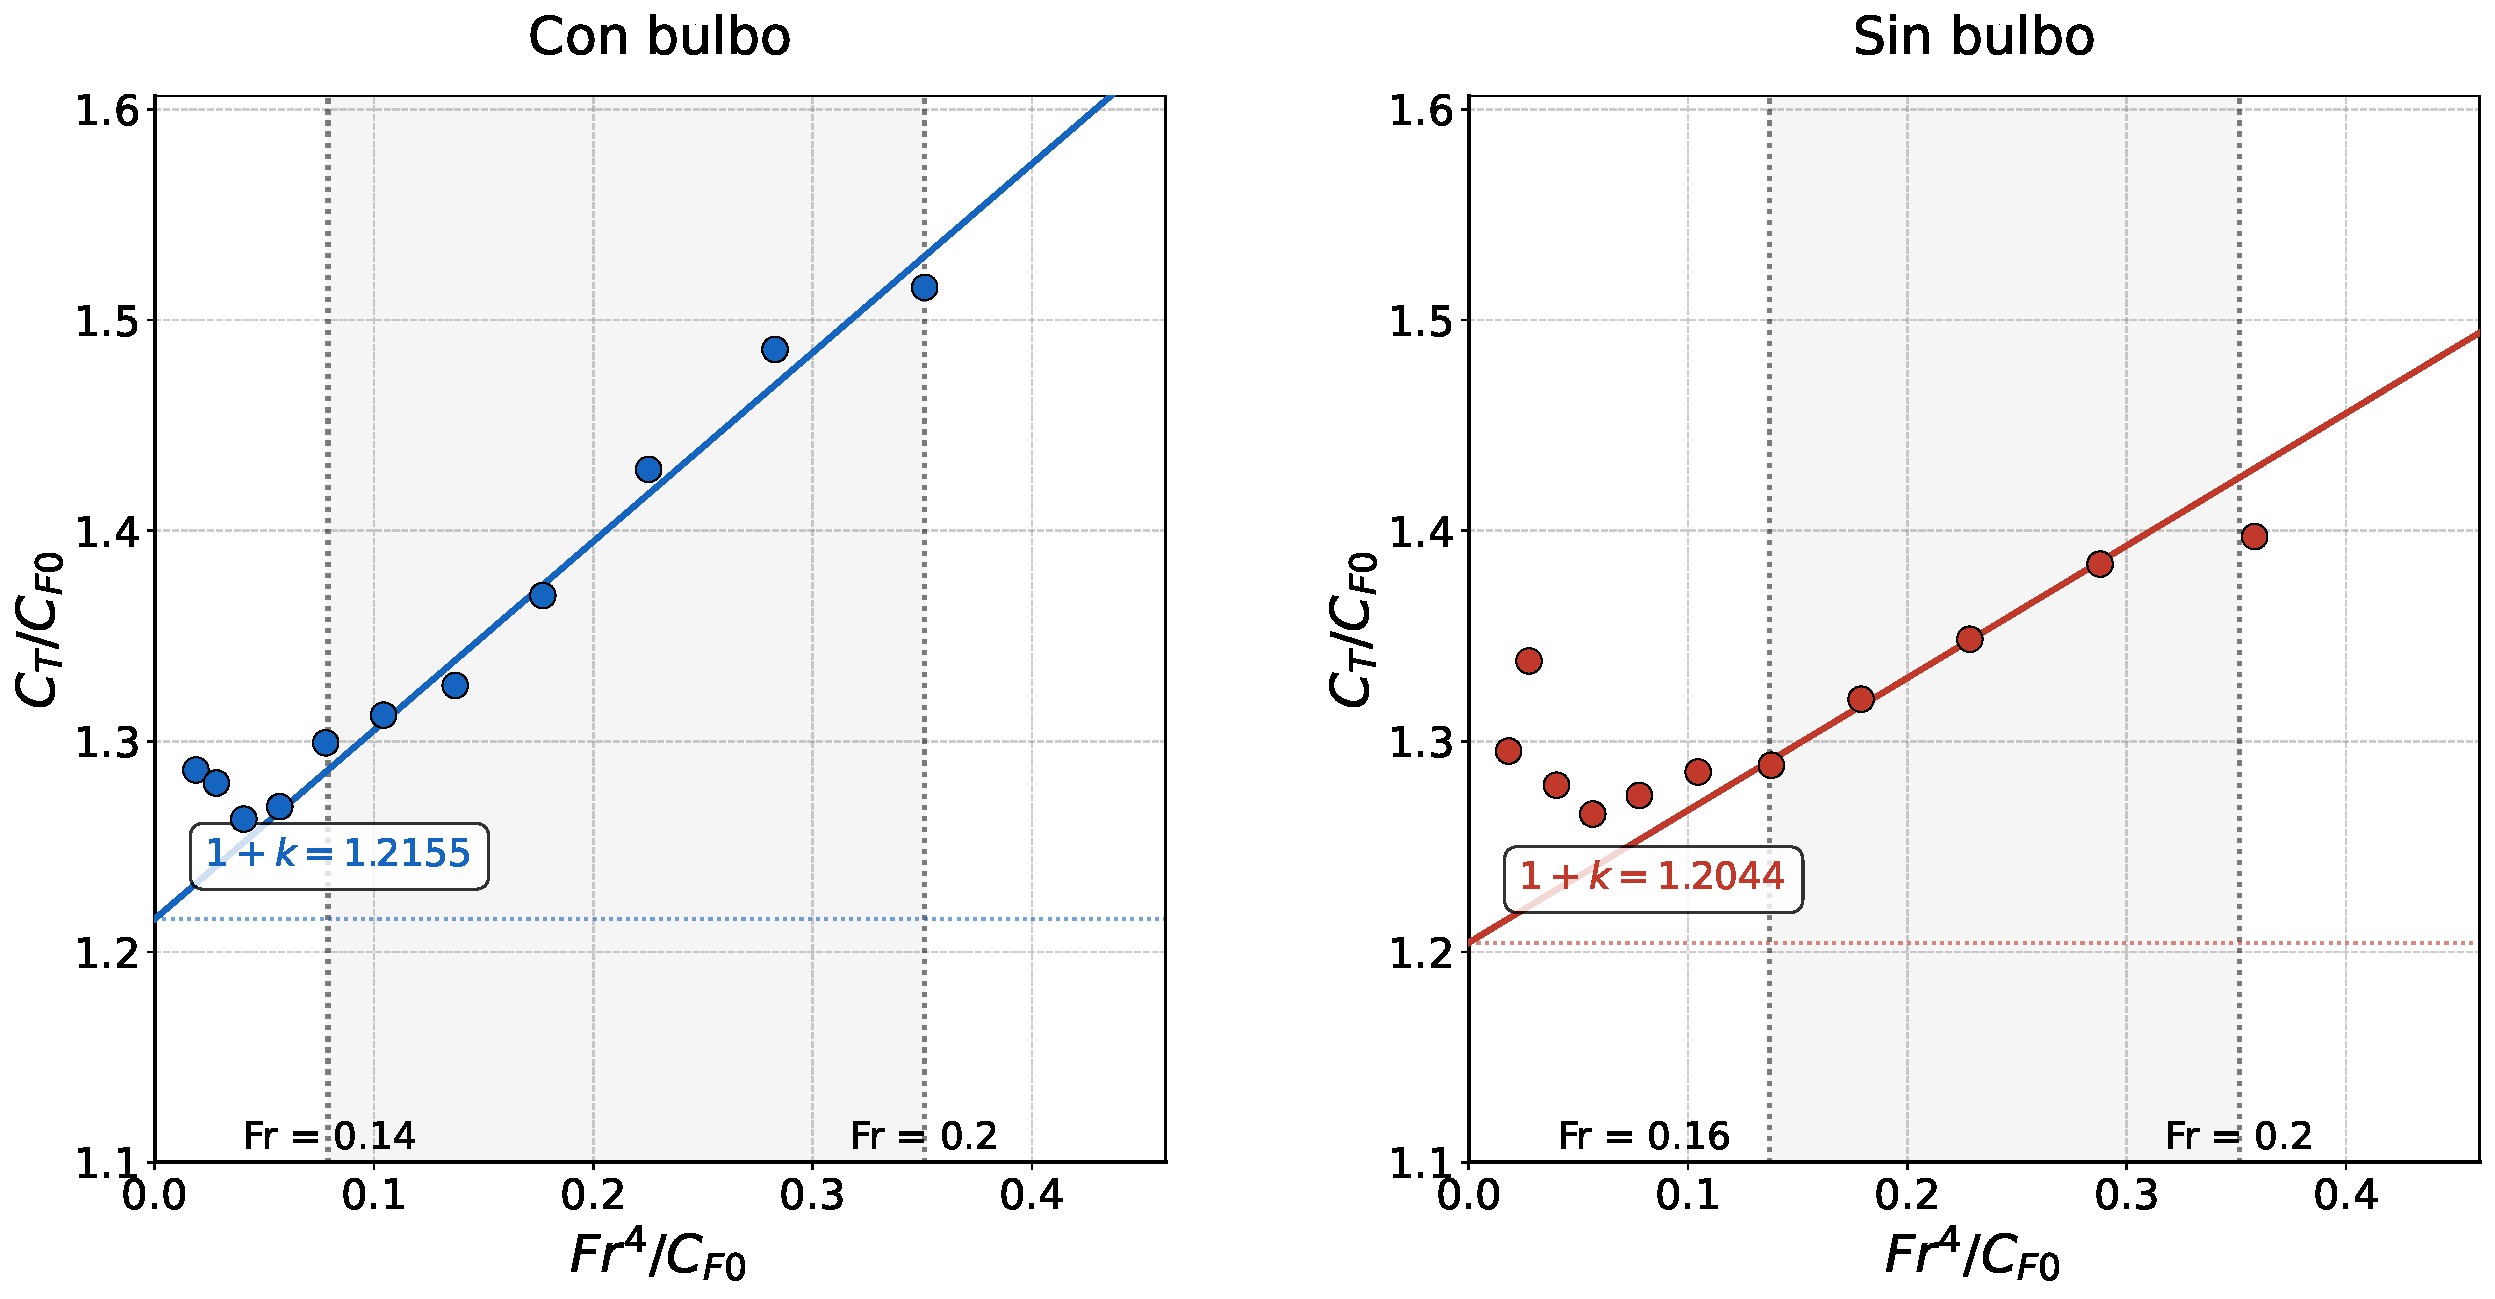
\includegraphics[width=.9\textwidth]{images/prohaska-bulbo-ctrlz-195.pdf}
	\caption{Diagrama de Prohaska comparando modelos con y sin bulbo 
	($T = 0{.}195$~m).}
	\label{fig:prohaska_bulbo_195}
\end{figure}

\paragraph{Calado $T = 0{.}165$~m} La Figura~\ref{fig:Ct_bulbo_165} muestra 
que la configuración con bulbo reduce la resistencia total a partir de 
$Fr \approx 0{.}25$, coincidiendo con la velocidad de diseño del bulbo. Por 
debajo de dicho valor ambas curvas se mantienen dentro de $5\times10^{-4}$ 
en $C_T$, sin diferencias apreciables entre configuraciones, con la 
excepción del punto $Fr \approx 0{.}24$, inmediatamente anterior al cruce, 
donde la configuración con bulbo presenta un incremento localizado de la 
resistencia total. La Figura~\ref{fig:Cw_bulbo_165} muestra que la mejora 
observada a velocidades altas se explica por una reducción de la resistencia 
por olas en ese mismo rango, consistente con la función destructiva esperada 
del bulbo. La Figura~\ref{fig:Cv_bulbo_165} muestra que la resistencia 
viscosa de la configuración con bulbo resulta levemente superior en todo el 
rango, entre un $1$ y un $1{.}5$\,\%, diferencia reducida pero de signo 
constante y consistente con el mayor factor de forma determinado para esta 
configuración.

\begin{figure}[htpb]
    \centering
    \begin{subfigure}[b]{0.48\textwidth}
        \centering
        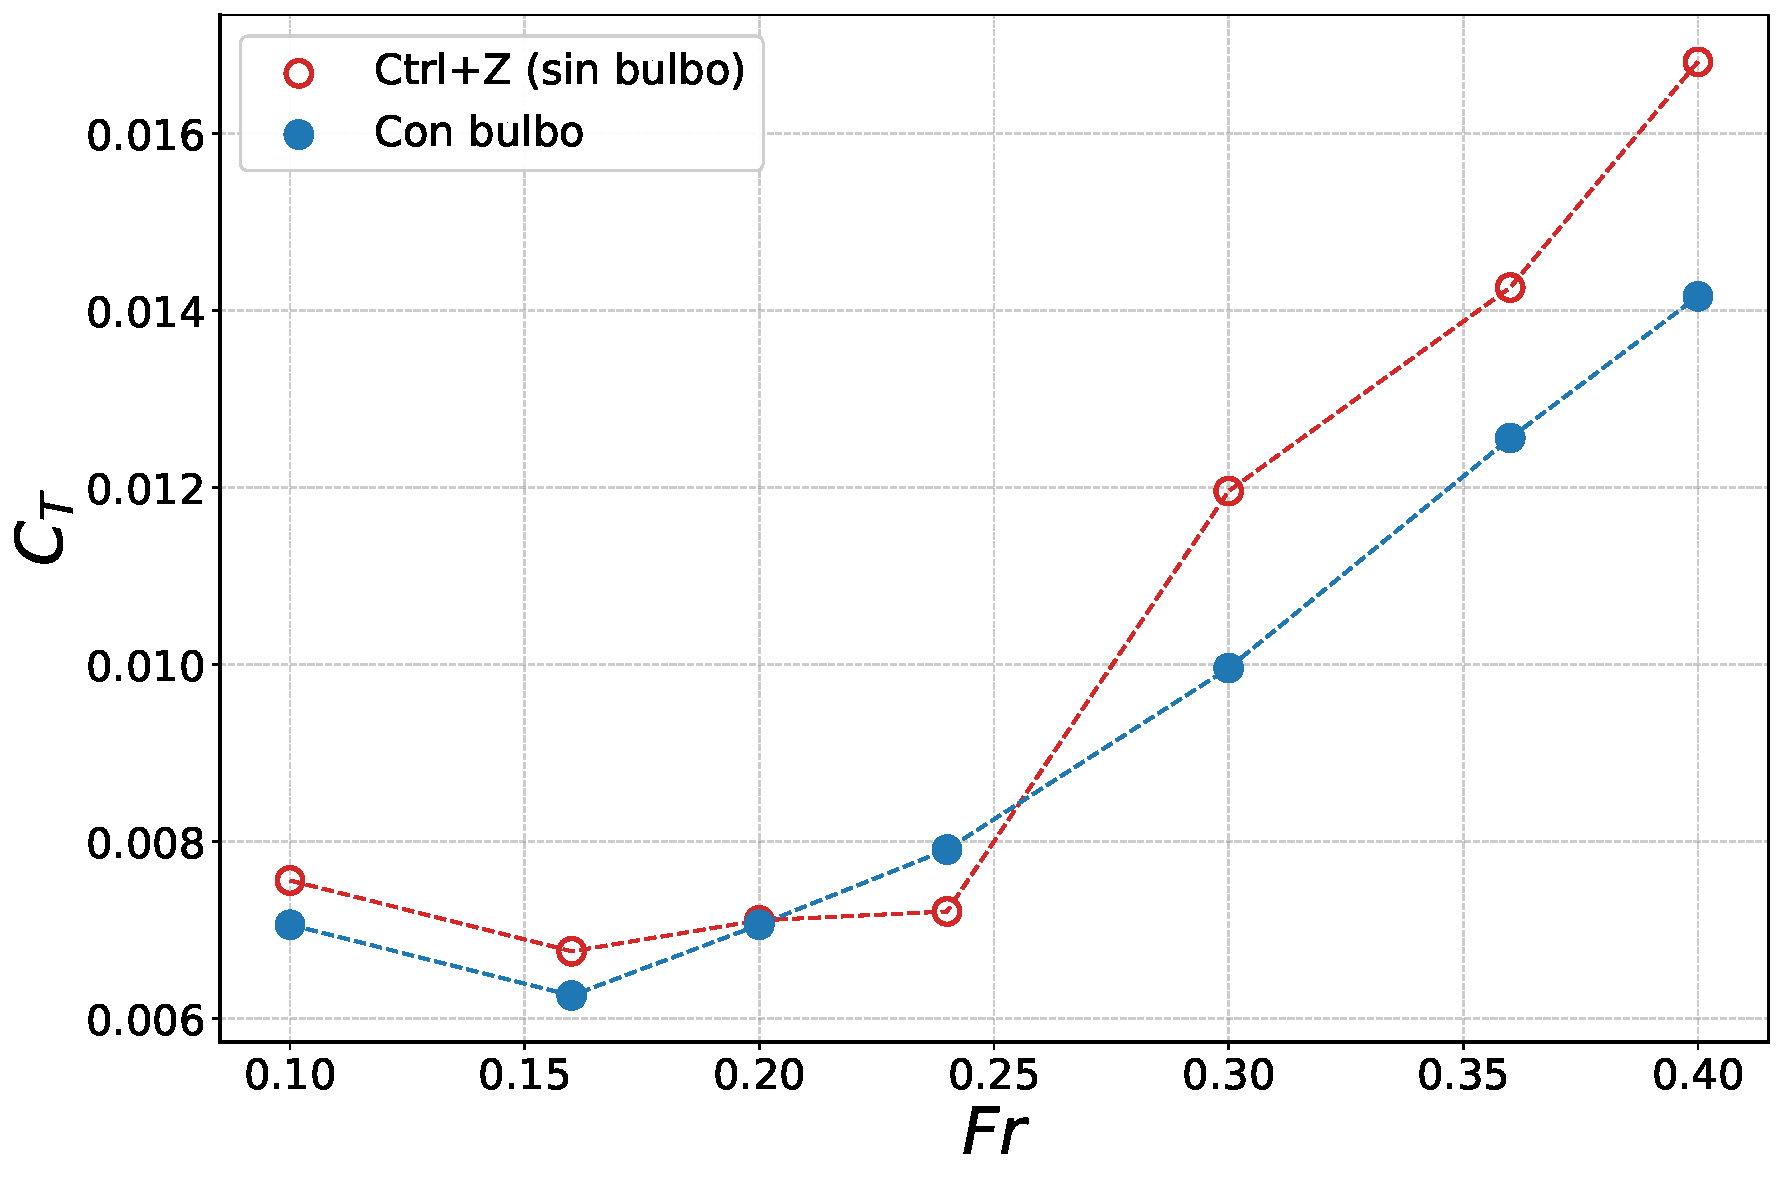
\includegraphics[width=\textwidth]{images/Ct-consinbulbo-165.pdf}
        \caption{Resistencia total.}
        \label{fig:Ct_bulbo_165}
    \end{subfigure}
    \hfill
    \begin{subfigure}[b]{0.48\textwidth}
        \centering
        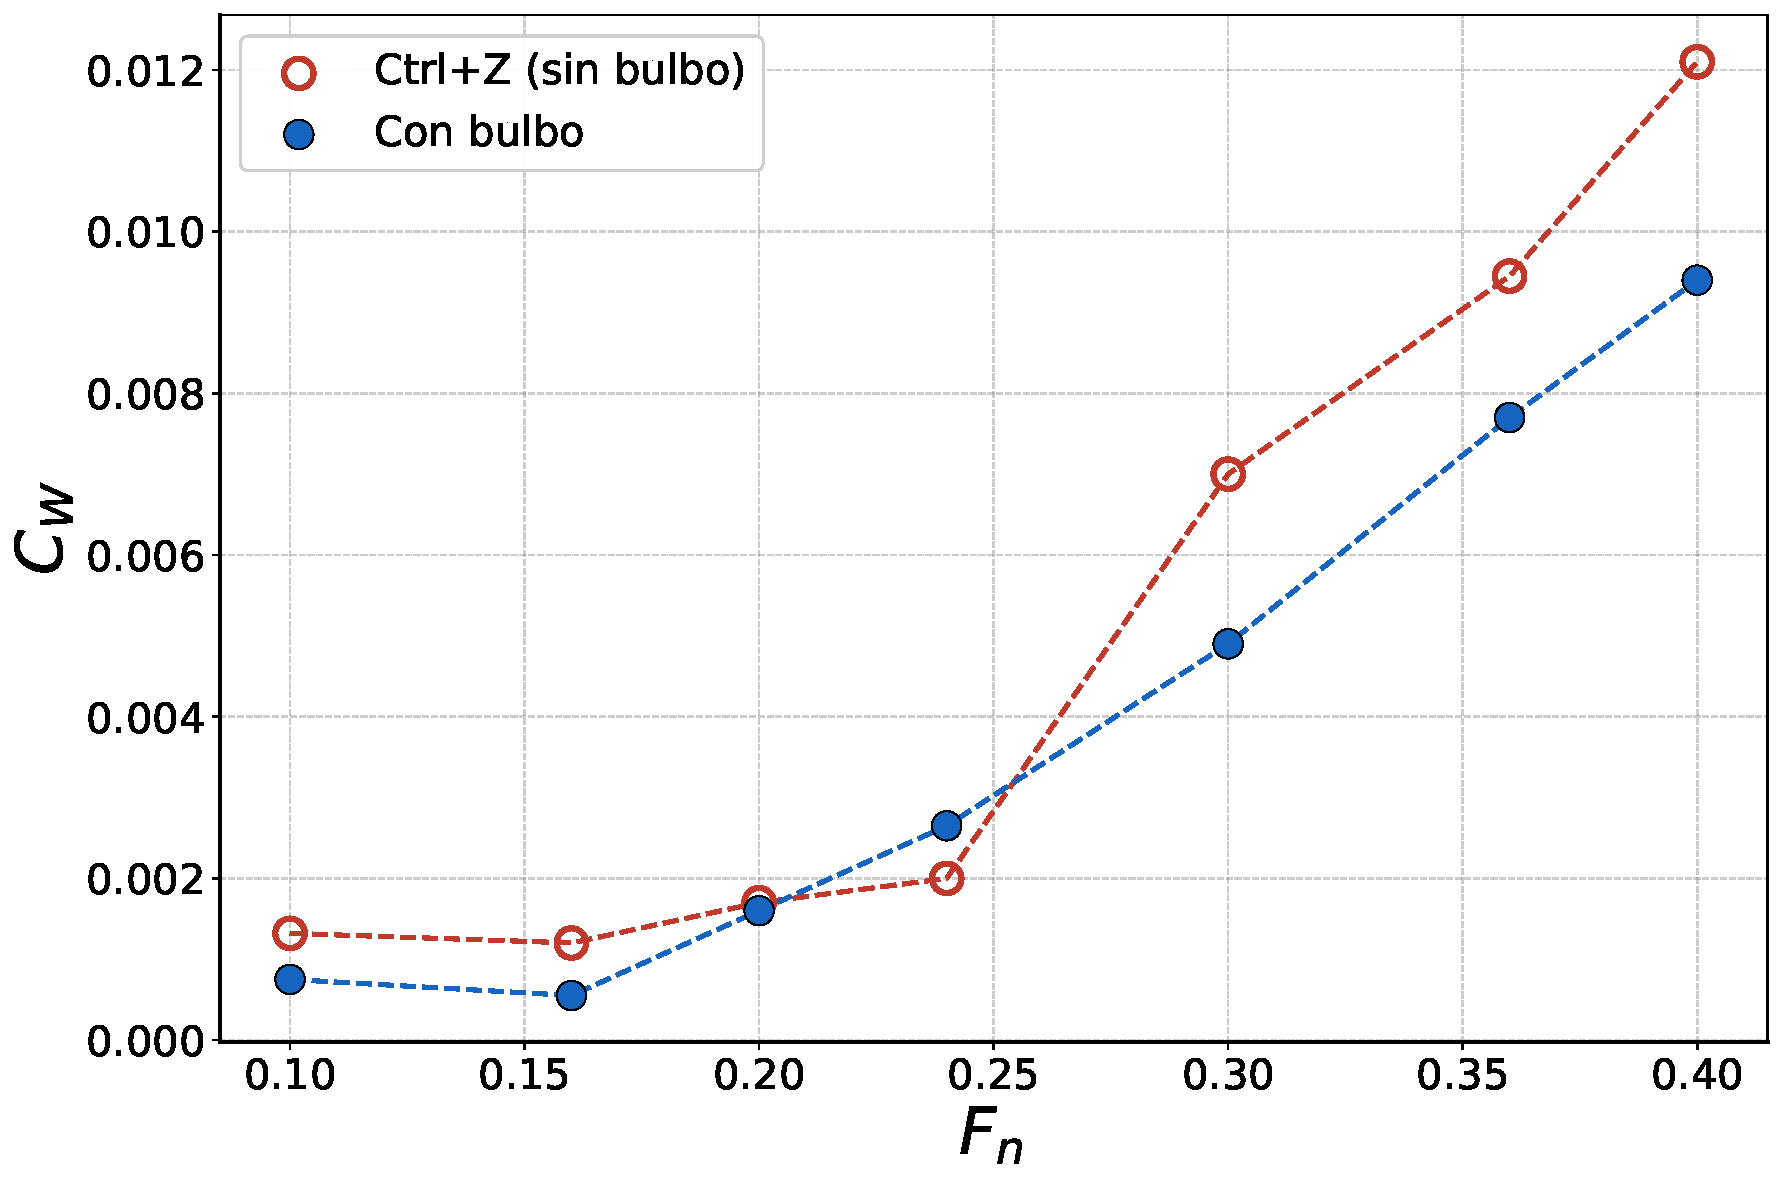
\includegraphics[width=\textwidth]{images/Cw-consinbulbo-165.pdf}
        \caption{Resistencia por olas.}
        \label{fig:Cw_bulbo_165}
    \end{subfigure}

    \vspace{0.6cm}

    \begin{subfigure}[b]{0.48\textwidth}
        \centering
        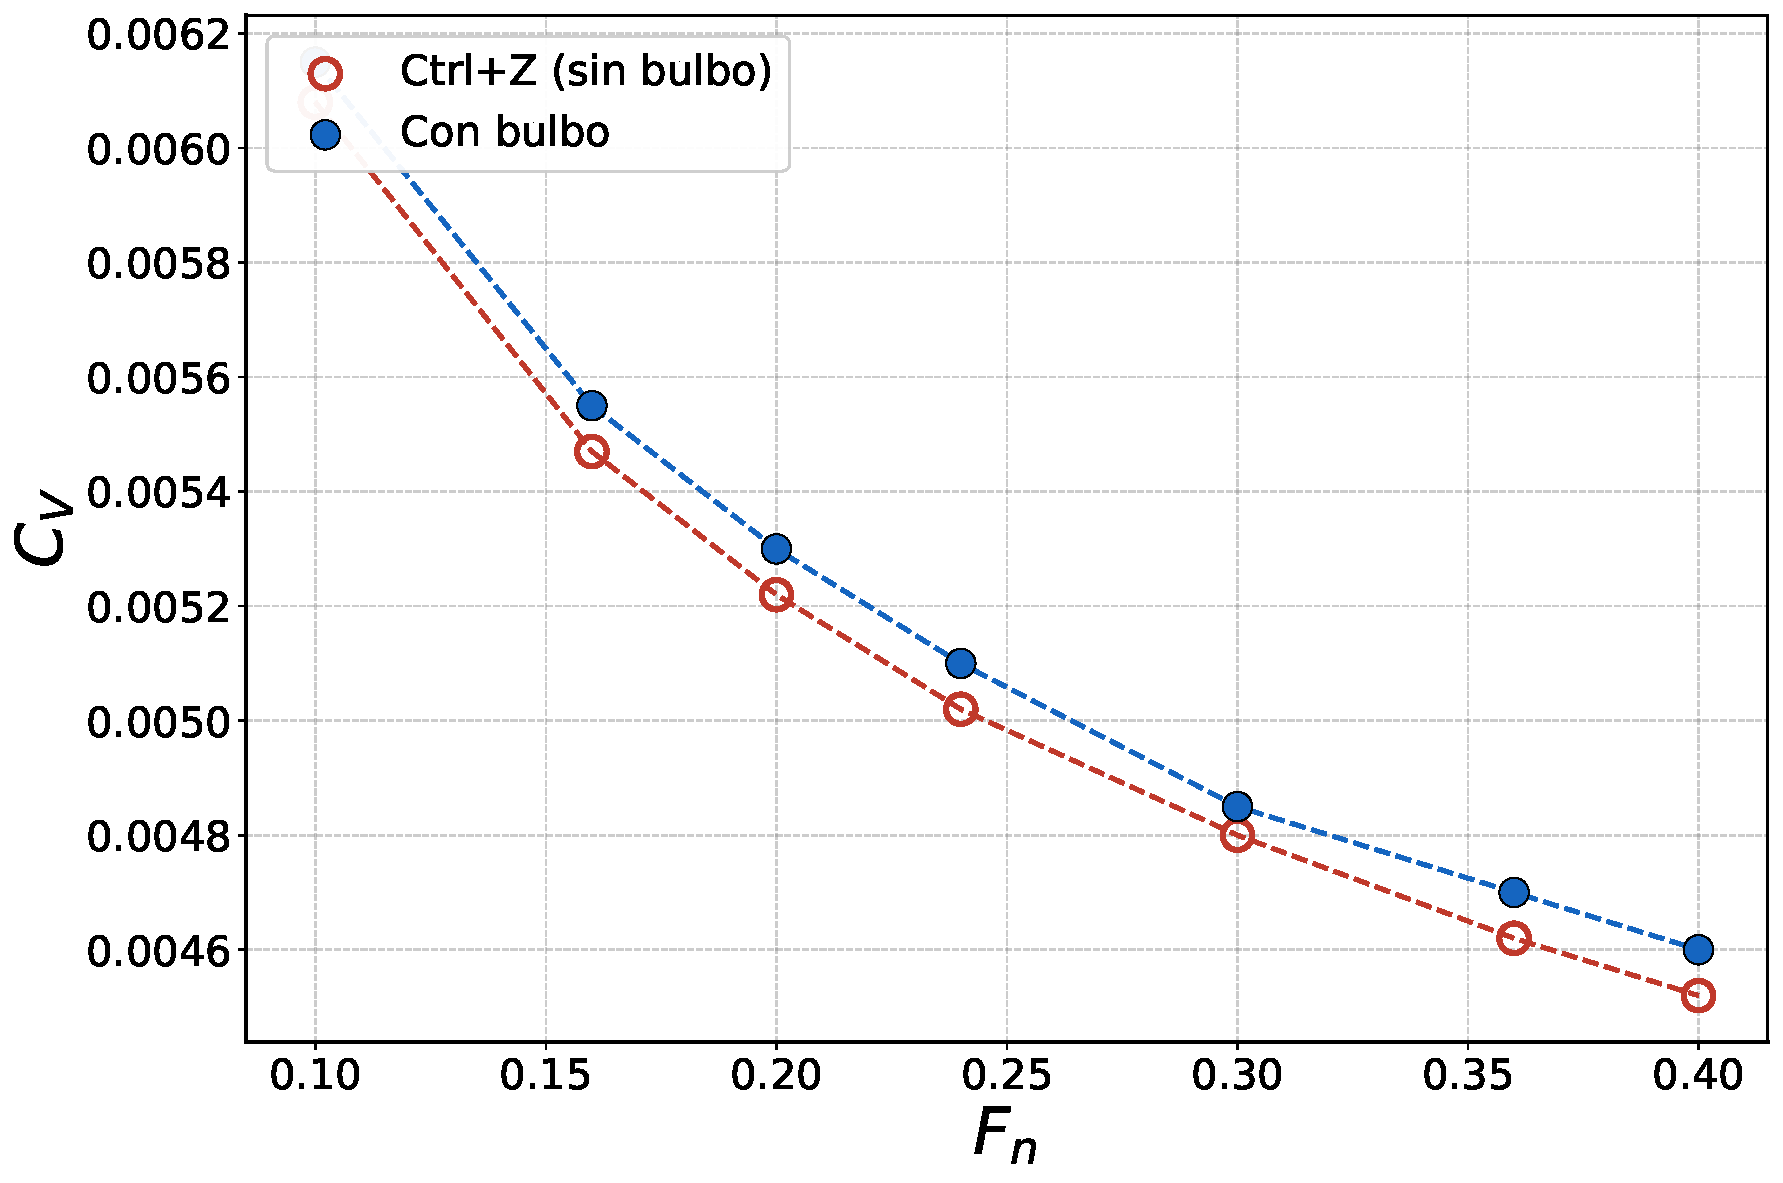
\includegraphics[width=\textwidth]{images/Cv-consinbulbo-165.pdf}
        \caption{Resistencia viscosa.}
        \label{fig:Cv_bulbo_165}
    \end{subfigure}

    \caption{Descomposición de la resistencia del \textit{P1} con y sin proa 
    bulbo para el calado $T = 0{.}165$~m.}
    \label{fig:coef_bulbo_165}
\end{figure}

\paragraph{Calado $T = 0{.}195$~m} Para este calado, la 
Figura~\ref{fig:Ct_bulbo_195} muestra que la configuración con bulbo no 
presenta una mejora neta en resistencia total: la diferencia entre ambas 
curvas oscila a lo largo del rango sin definir una tendencia, alternando 
tramos favorables y desfavorables al bulbo. La 
Figura~\ref{fig:Cv_bulbo_195} muestra que las resistencias viscosas de ambas 
configuraciones resultan prácticamente indistinguibles, de modo que la 
diferencia observada en $C_T$ se explica enteramente por la componente de 
olas. En efecto, la Figura~\ref{fig:Cw_bulbo_195} muestra que el bulbo 
reduce $C_W$ en el entorno de $Fr \approx 0{.}20$--$0{.}30$, pero pierde 
ese beneficio por encima de $Fr \approx 0{.}35$, donde la tendencia se 
invierte y la configuración con bulbo pasa a presentar una resistencia por 
olas superior a la del casco desnudo.

Este comportamiento resulta consistente con la mayor sumergencia del bulbo a 
este calado. Al aumentar su distancia a la superficie libre se modifica el 
sistema de ondas que genera, tanto en amplitud como en fase, de manera que 
la interferencia destructiva con el tren de olas del casco deja de resultar 
favorable en el extremo alto del rango de operación. El beneficio 
hidrodinámico del bulbo aparece así como fuertemente dependiente de la 
condición de carga.

\begin{figure}[htpb]
    \centering
    \begin{subfigure}[b]{0.48\textwidth}
        \centering
        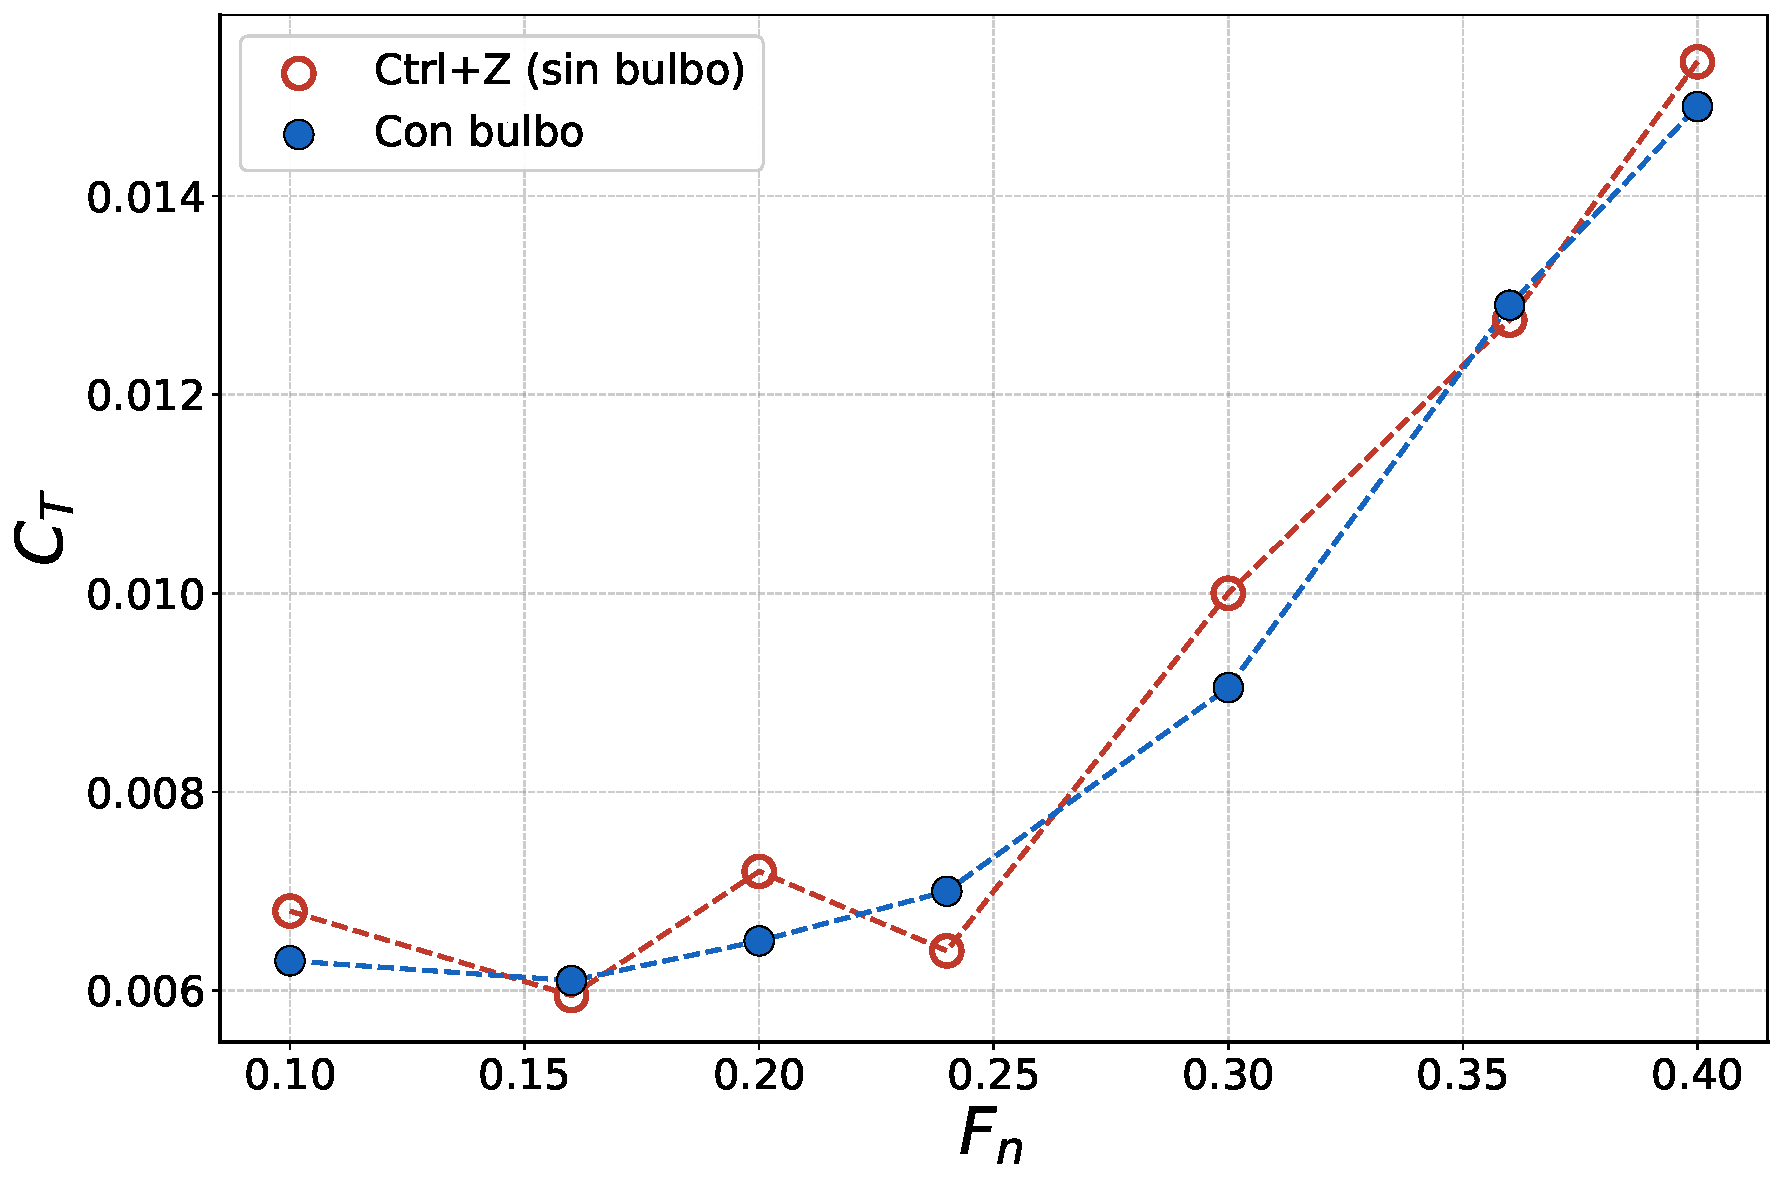
\includegraphics[width=\textwidth]{images/Ct-consinbulbo-195.pdf}
        \caption{Resistencia total.}
        \label{fig:Ct_bulbo_195}
    \end{subfigure}
    \hfill
    \begin{subfigure}[b]{0.48\textwidth}
        \centering
        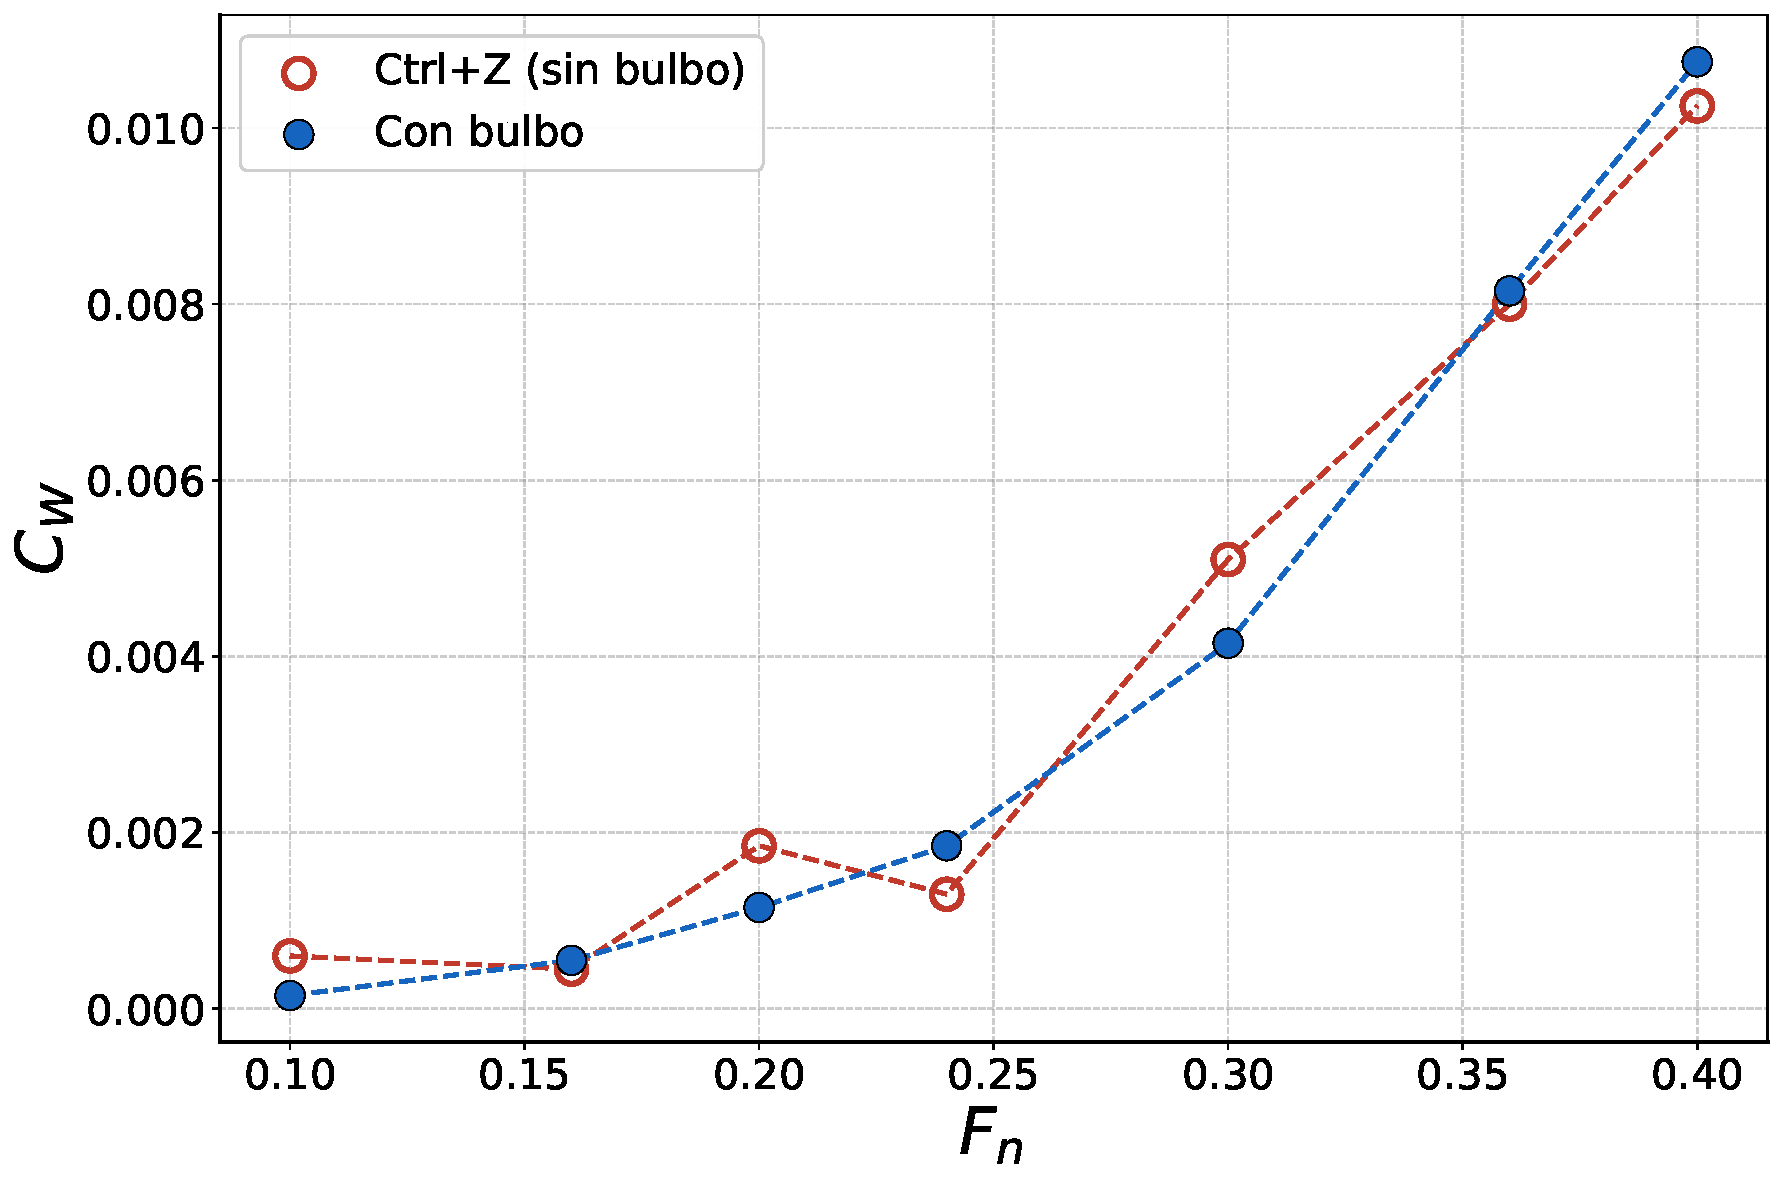
\includegraphics[width=\textwidth]{images/Cw-consinbulbo-195.pdf}
        \caption{Resistencia por olas.}
        \label{fig:Cw_bulbo_195}
    \end{subfigure}

    \vspace{0.6cm}

    \begin{subfigure}[b]{0.48\textwidth}
        \centering
        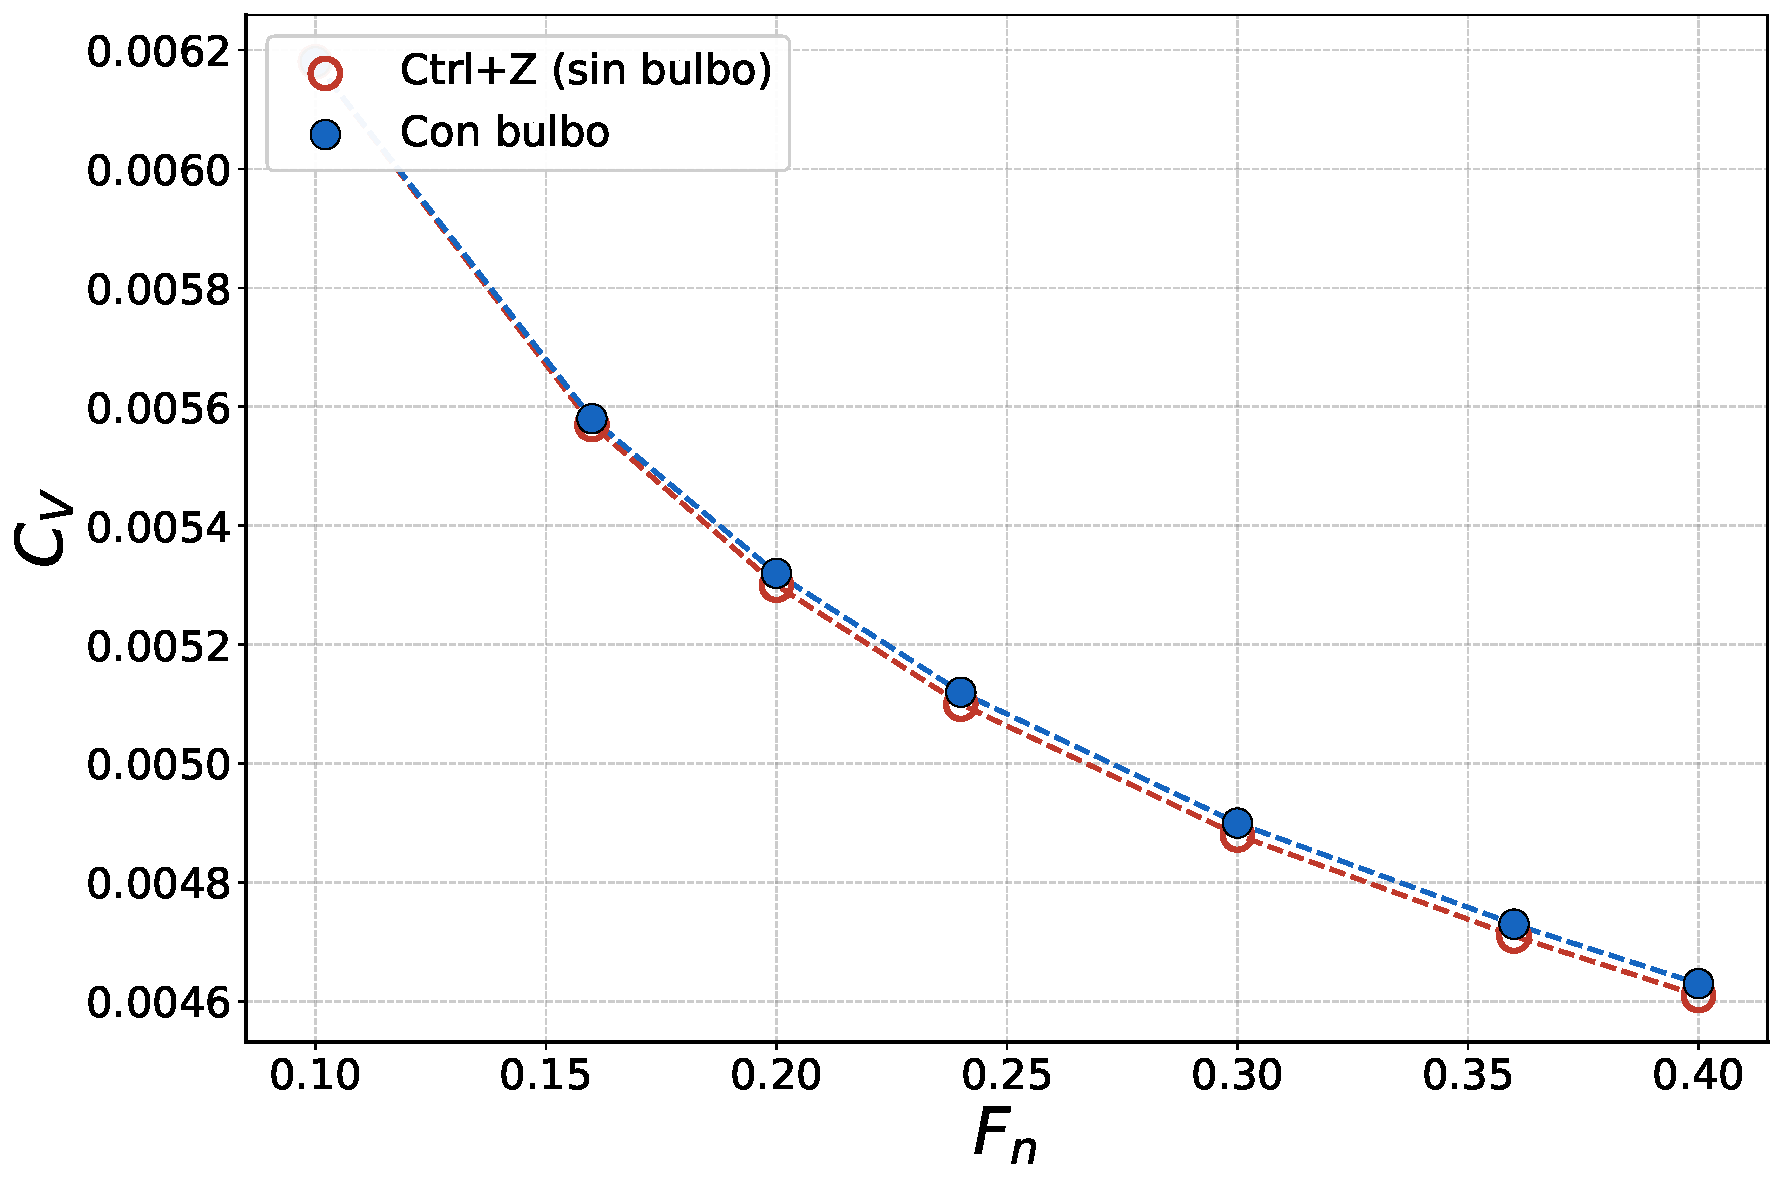
\includegraphics[width=\textwidth]{images/Cv-consinbulbo-195.pdf}
        \caption{Resistencia viscosa. Ambas configuraciones resultan 
        indistinguibles en todo el rango.}
        \label{fig:Cv_bulbo_195}
    \end{subfigure}

    \caption{Descomposición de la resistencia del \textit{P1} con y sin proa 
    bulbo para el calado $T = 0{.}195$~m.}
    \label{fig:coef_bulbo_195}
\end{figure}

Estos resultados, desde el punto de vista hidrodinámico, obligan a repensar 
el diseño de la proa de los pesqueros. Sin embargo, como fue mencionado en 
la introducción, el bulbo ayuda a aumentar la capacidad de carga del buque. 
Aunque su efecto hidrodinámico pueda ser desfavorable según el calado, es 
posible que el análisis económico muestre que la ganancia en capacidad de 
carga supere la pérdida asociada a un diseño no optimizado 
hidrodinámicamente.

\subsection{Efecto sobre el factor de forma}

\paragraph{Efecto sobre el valor de $(1+k)$} La aplicación del método de 
Prohaska a las simulaciones bifásicas de ambas configuraciones arroja los 
valores reunidos en la Tabla~\ref{tab:k_bulbo_ctrlz}. El bulbo incrementa el 
factor de forma en los dos calados analizados, lo cual es consistente con el 
aumento de resistencia por presión viscosa asociado a un cuerpo adicional en 
la proa. La magnitud del efecto, sin embargo, difiere de manera marcada 
entre condiciones de carga: mientras que a $T = 0{.}165$~m el incremento 
alcanza el $3{.}0$\,\%, a $T = 0{.}195$~m se reduce a $0{.}9$\,\%.

\begin{table}[htpb]
\centering
\caption{Factor de forma $(1+k)$ obtenido por el método de Prohaska para 
ambas configuraciones de proa, junto con el rango de $Fr$ empleado en cada 
regresión.}
\label{tab:k_bulbo_ctrlz}
\begin{tabular}{llcc}
\hline
Calado & Configuración & Rango de $Fr$ & $(1+k)$ \\
\hline
\multirow{2}{*}{$T = 0{.}165$~m} & Con bulbo & $0{.}13$--$0{.}20$ & $1{.}204$ \\
                                 & Ctrl+Z    & $0{.}14$--$0{.}20$ & $1{.}169$ \\
\hline
\multirow{2}{*}{$T = 0{.}195$~m} & Con bulbo & $0{.}14$--$0{.}20$ & $1{.}215$ \\
                                 & Ctrl+Z    & $0{.}16$--$0{.}20$ & $1{.}204$ \\
\hline
\end{tabular}
\end{table}

Esta dependencia con el calado resulta coherente con el mecanismo propuesto 
en la literatura: si la contribución del bulbo al factor de forma está 
asociada a su proximidad a la superficie libre, al aumentar el calado el 
bulbo queda más sumergido y su influencia se atenúa. El resultado es 
consistente, además, con el comportamiento de la componente de olas descrito 
en la subsección anterior, donde el beneficio del bulbo también se 
desvanecía al aumentar el calado.

\paragraph{Efecto sobre la tendencia de $(1+k)$ con la velocidad} La 
comparación de las curvas de $(1+k)$ determinadas por doble cuerpo 
(Figuras~\ref{fig:k_bulbo_165} y \ref{fig:k_bulbo_195}) permite abordar la 
segunda de las hipótesis planteadas. Ambas configuraciones presentan un 
crecimiento sostenido de $(1+k)$ con la velocidad, de magnitud comparable, 
sin alcanzar un valor asintótico en el rango analizado. El bulbo desplaza 
las curvas hacia valores mayores, en línea con lo indicado en la 
Tabla~\ref{tab:k_bulbo_ctrlz}, pero no introduce ni modifica 
sustancialmente la tendencia creciente.

Cabe señalar que la determinación por doble cuerpo del casco con bulbo debe 
interpretarse con cautela en cuanto a sus valores absolutos, dado que la 
condición de simetría impuesta en la frontera superior del dominio puede 
distorsionar el campo de presiones en la zona de proa cuando el bulbo se 
encuentra próximo a dicha frontera, tal como se discutió en la 
Sección~\ref{sec:cfd_ff_antec}. El análisis presentado aquí se apoya, por lo 
tanto, en la comparación de tendencias entre configuraciones y no en el 
nivel absoluto de cada curva.

\begin{figure}[htpb]
    \centering
    \begin{subfigure}[b]{0.48\textwidth}
        \centering
        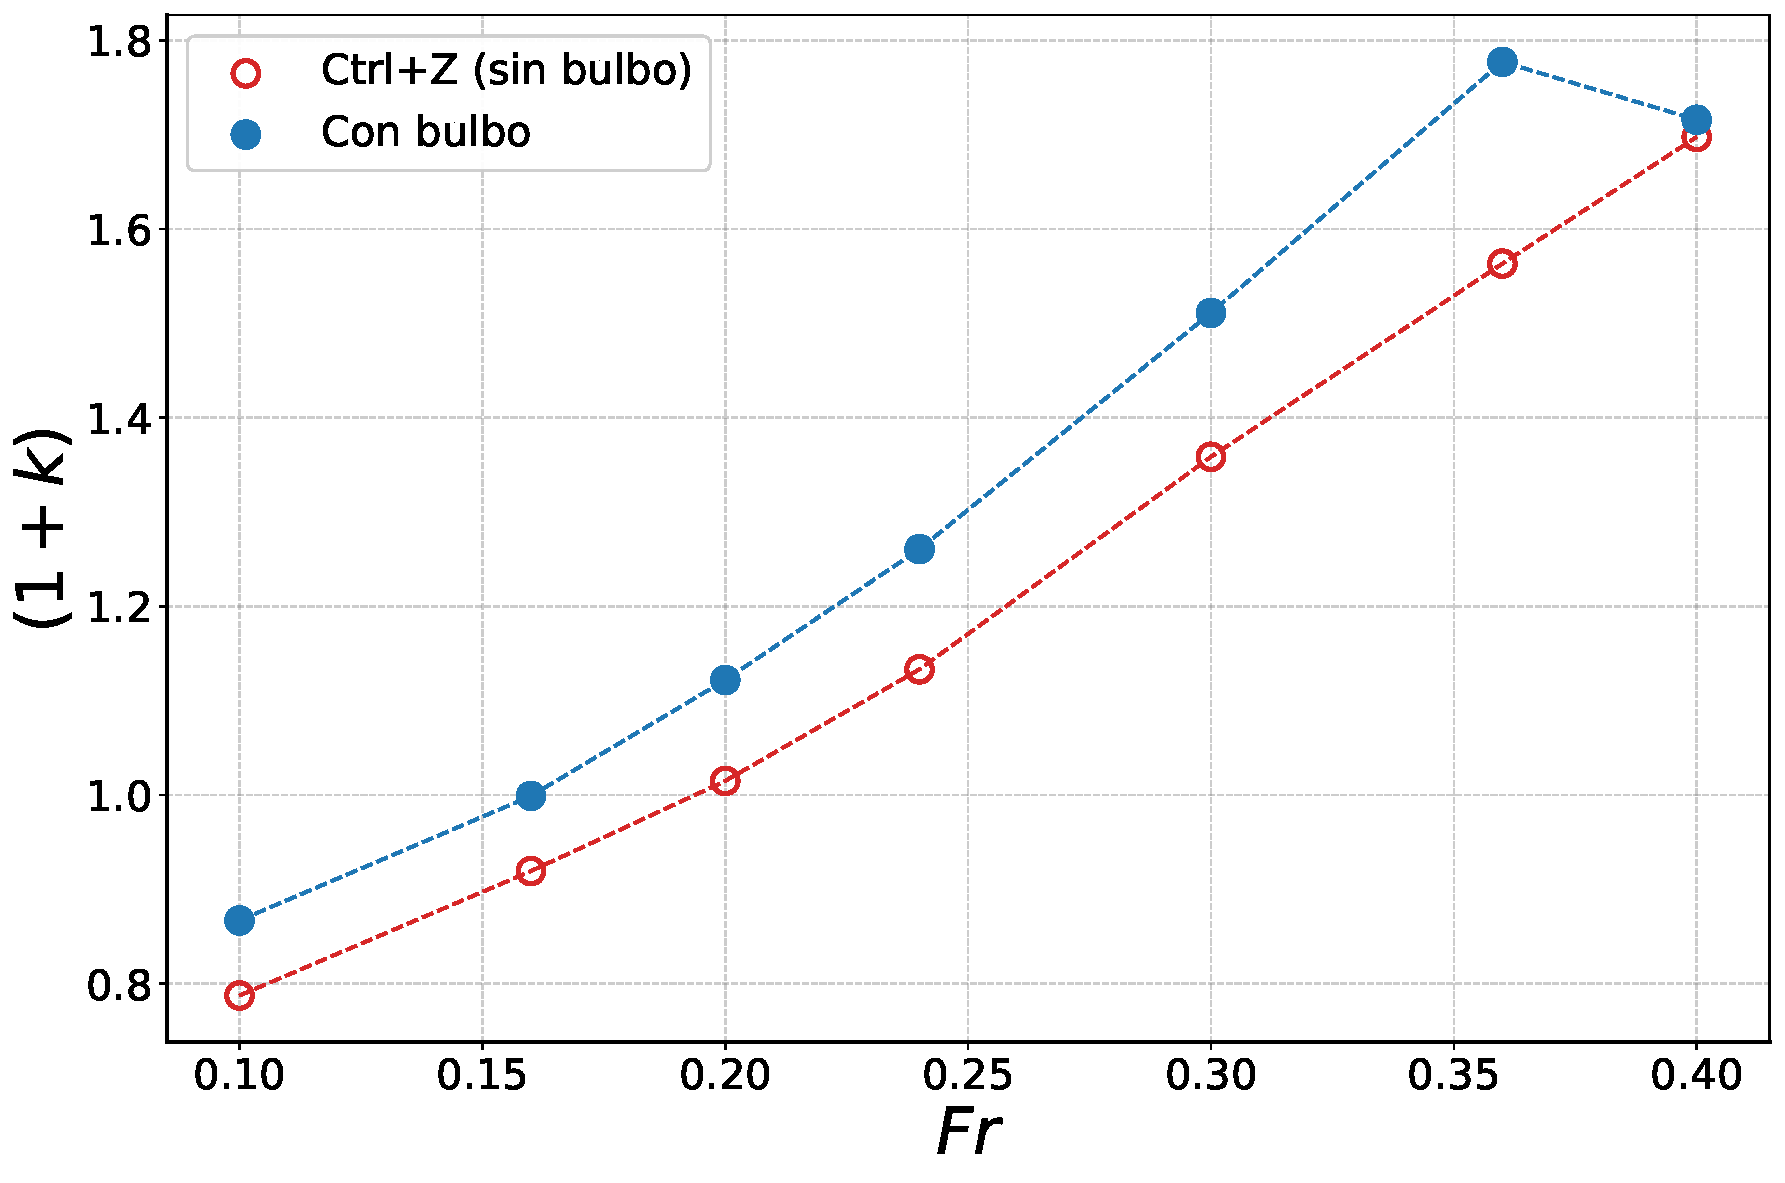
\includegraphics[width=\textwidth]{images/k-consinbulbo-165.pdf}
        \caption{$T = 0{.}165$~m.}
        \label{fig:k_bulbo_165}
    \end{subfigure}
    \hfill
    \begin{subfigure}[b]{0.48\textwidth}
        \centering
        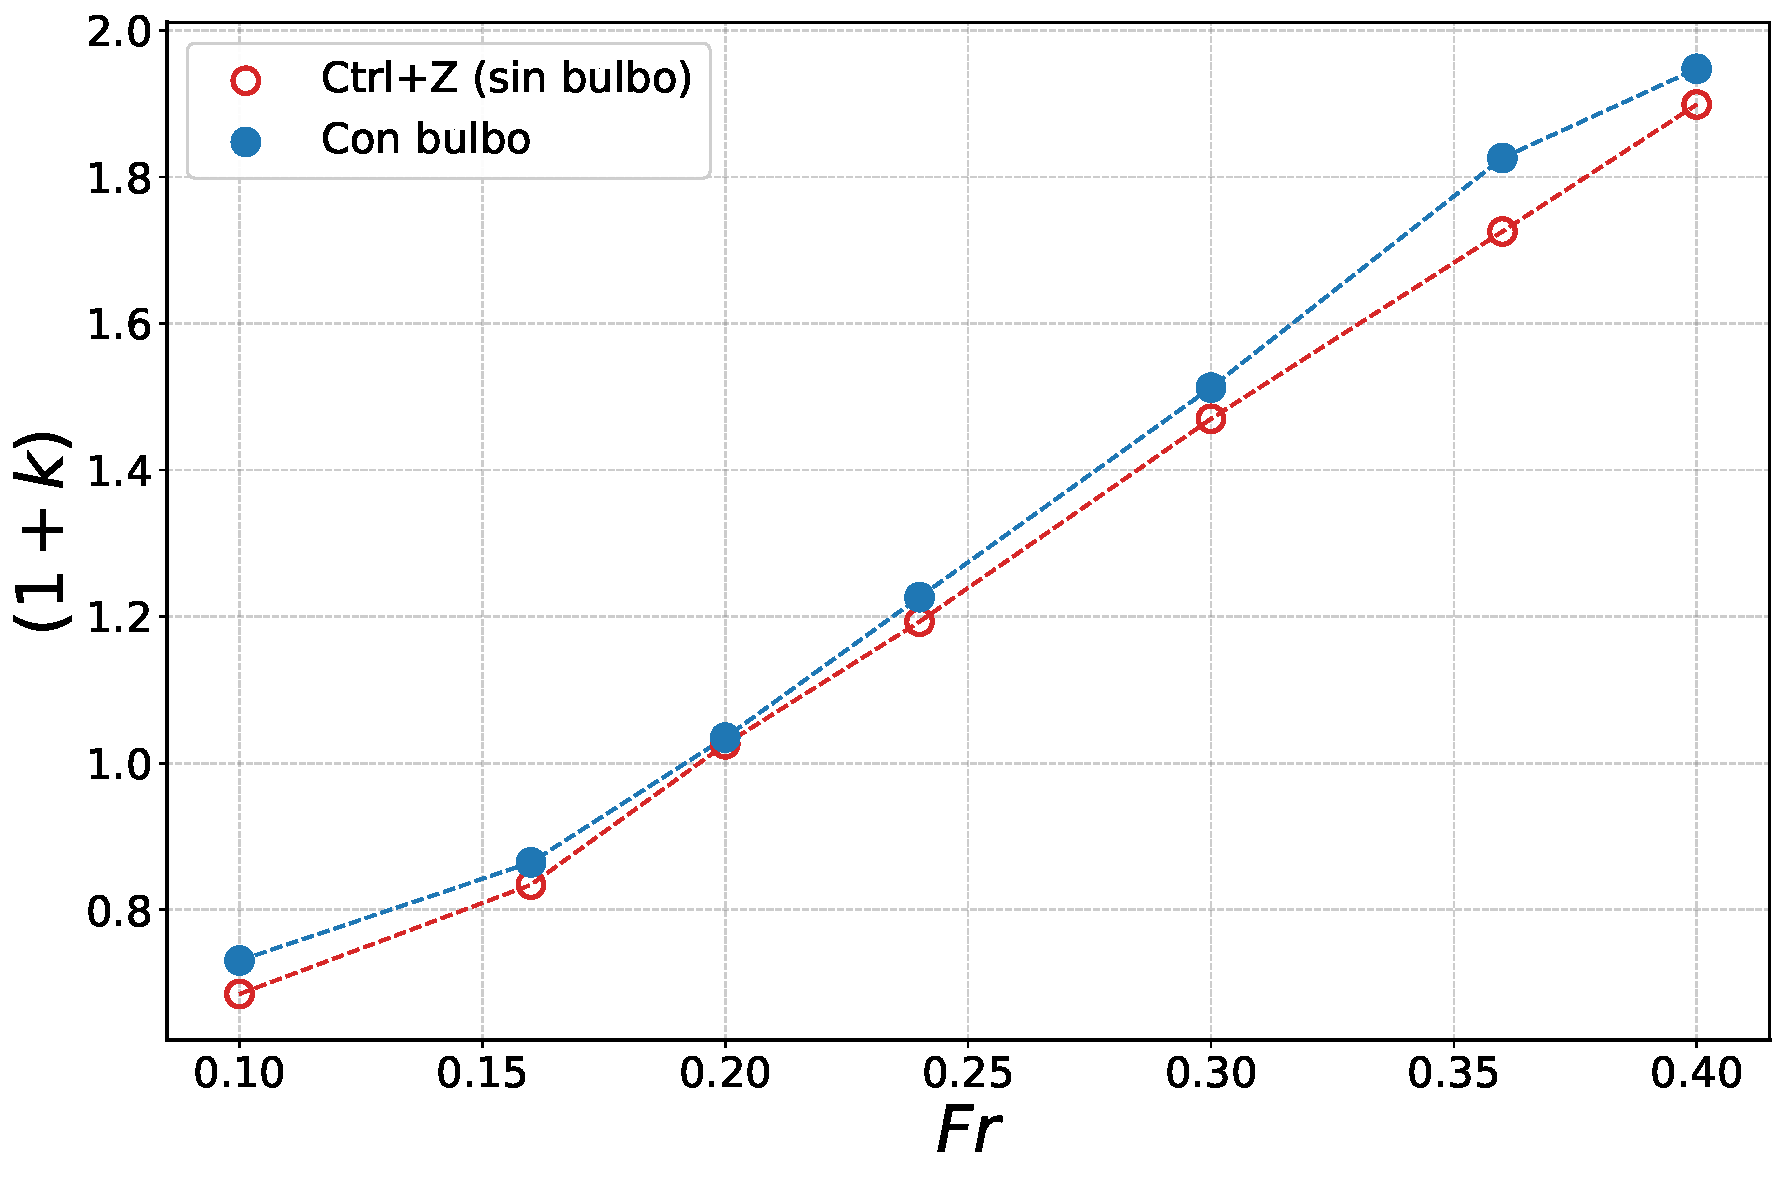
\includegraphics[width=\textwidth]{images/k-consinbulbo-195.pdf}
        \caption{$T = 0{.}195$~m.}
        \label{fig:k_bulbo_195}
    \end{subfigure}

    \caption{Factor de forma $(1+k)$ del \textit{P1} con y sin proa bulbo en 
    función del número de Froude, para ambos calados.}
    \label{fig:k_bulbo}
\end{figure}

\subsection{Conclusiones parciales}

El análisis comparativo entre el \textit{P1} y su variante sin bulbo 
permite extraer tres conclusiones.

En primer lugar, el bulbo modifica el valor del factor de forma determinado 
por el método de Prohaska, incrementándolo en ambos calados, con un efecto 
tres veces mayor en la condición de carga ligera que en la pesada. Esta 
dependencia con el calado es consistente con un mecanismo gobernado por la 
proximidad del bulbo a la superficie libre.

En segundo lugar, el bulbo incrementa la resistencia viscosa y reduce la 
resistencia por olas dentro de su rango de diseño, pero el balance resultante 
depende fuertemente de la condición de carga. A calado reducido resulta 
favorable para la resistencia total por encima de $Fr \approx 0{.}25$, 
mientras que a mayor calado el beneficio desaparece e incluso se invierte en 
el extremo alto del rango de operación.

En tercer lugar, y respecto de la pregunta que motivó este análisis, ni la 
curvatura del diagrama de Prohaska a bajos números de Froude ni la ausencia 
de estabilización de $(1+k)$ con la velocidad pueden atribuirse a la 
presencia del bulbo: ambos comportamientos persisten de manera análoga en el 
modelo Ctrl+Z. Este resultado descarta al bulbo como causa principal y 
refuerza la necesidad de buscar dicha causa en otras características 
geométricas del casco, como su baja relación $L/B$, analizada en la 
Sección~\ref{sec:generalizacion_LB}. Cabe precisar que, en el caso 
particular de la curvatura del diagrama de Prohaska, el análisis aquí 
presentado descarta al bulbo pero no permite distinguir entre un origen 
geométrico y uno numérico asociado al modelado de la transición, dado que 
ambas configuraciones comparten el mismo cierre turbulento.

\section{Influencia de la popa sumergida en el factor de forma}\label{sec:popa_sumergida}

\subsection{Introducción y motivación del estudio}

El estudio de \cite{korkmaz_wetted_transom} analiza la influencia del flujo con \textit{popa mojada} (\textit{wetted-transom flow}) sobre la predicción de la resistencia total y la extrapolación ITTC--78.  
Cuando el espejo de la popa se encuentra sustancialmente sumergido, ya sea por operar a baja velocidad o por calados elevados, se forma una \textbf{zona de recirculación} detrás del espejo, análoga al flujo que ocurre sobre un \textit{backward-facing step} o \textit{escalón hacia atrás}.  
En este régimen, la presión en la arista del espejo no alcanza el valor atmosférico, el flujo se separa y se genera una región de baja presión con un vórtice persistente aguas abajo.

\subsection{Definiciones geométricas y parámetros característicos}

Para describir el grado de inmersión del espejo, \cite{korkmaz_wetted_transom} definió una serie de parámetros adimensionales (Fig.~\ref{fig:transom_defs}), los cuales se expresan mediante las siguientes relaciones:

\begin{equation}
Fr_{tr} = \frac{V}{\sqrt{g\,T_{tr}}}
\end{equation}

\begin{equation}
tr_{\mathrm{ratio}} = \frac{A_{tr}}{A_{\max}}
\end{equation}

\begin{equation}
tr_{\mathrm{fullness}} = \frac{A_{tr}}{2\,y_{tr}\,T_{tr}}
\end{equation}

donde:
\begin{itemize}
  \item $A_{tr}$ es el área del espejo sumergido,
  \item $A_{\max}$ es el área máxima de la sección transversal,
  \item $y_{tr}$ es la mitad de la manga en la intersección del espejo con la superficie libre,
  \item $T_{tr}$ es la inmersión efectiva del borde inferior del espejo,
  \item $T$ el calado total del buque, y
  \item $V$ la velocidad correspondiente a la condición de análisis.
\end{itemize}

El número de Froude del transom $Fr_{tr}$ representa una medida del grado de ``seco o mojado'' del espejo:  
valores bajos indican flujo recirculante (popa mojada), mientras que valores altos ($Fr_{tr} > 3$) corresponden a popas secas o parcialmente mojadas.

\begin{figure}[htpb]
\centering
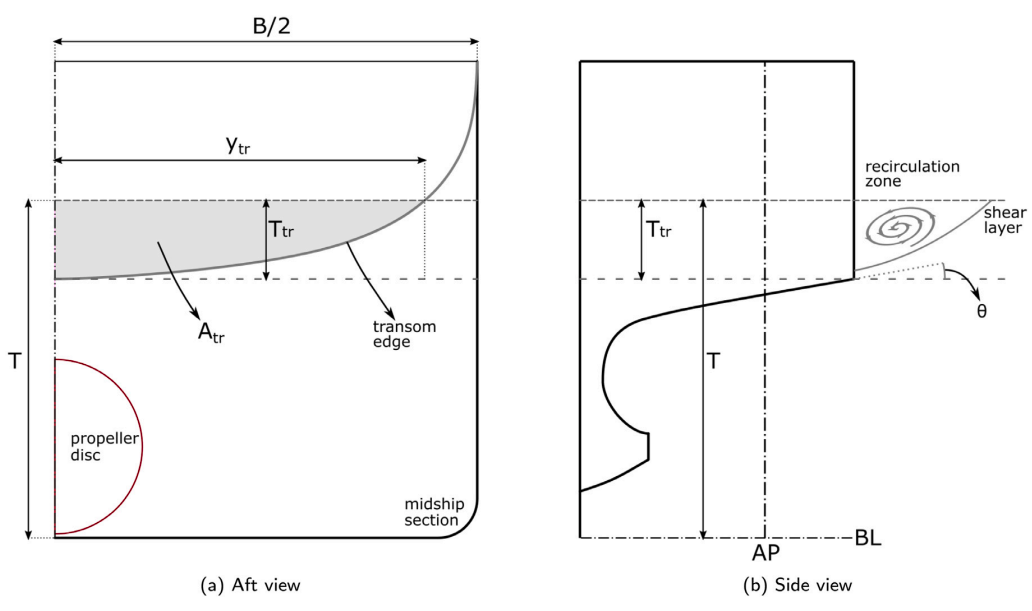
\includegraphics[width=.65\columnwidth]{images/transom_scheme.png}
\caption{Esquema de los parámetros geométricos de popa sumergida, adaptado de \cite{korkmaz_wetted_transom}.}
\label{fig:transom_defs}
\end{figure}

\subsection{Desarrollo del método 2--$k$}

El método \textit{two-form-factor} o 2--$k$ fue propuesto para corregir el déficit de resistencia viscosa generado por la recirculación en popas sumergidas.  
El procedimiento parte de la descomposición clásica de la resistencia viscosa total:

\begin{equation}
C_{V} = (1 + k)\,C_{F0}
\end{equation}

donde $C_{F0}$ es el coeficiente de fricción de ITTC-57 y $(1+k)$ el factor de forma convencional.  
En el caso de popas mojadas, el término $k$ se descompone en dos:

\begin{equation}
k_S = k_M + k_{tr}
\end{equation}

siendo $k_M$ el factor de forma obtenido para el modelo (por método de Prohaska o CFD doble cuerpo), y $k_{tr}$ un incremento asociado al flujo recirculante detrás del espejo, denominado \textit{transom form factor}.  
Este último se expresa como:

\begin{equation}
k_{tr} \simeq \frac{C_{tr,S}}{C_{F,S}}
\end{equation}

donde $C_{tr,S}$ representa la contribución viscosa adicional debida al vórtice de recirculación, y $C_{F,S}$ el coeficiente de fricción a escala buque.

El valor de $k_{tr}$ puede estimarse empíricamente mediante correlaciones con parámetros geométricos del espejo (secciones 6.3 y 7 de \cite{korkmaz_wetted_transom}) o mediante CFD comparativo entre modelo y escala buque:

\begin{equation}
k_{tr} = k_S - k_M
\end{equation}

Este punto es clave, ya que en \citet{korkmaz_wetted_transom} se atribuye la diferencia entre el factor de forma en escala modelo y en escala buque, en los casos de popa espejo sumergida, principalmente al flujo recirculante detrás del espejo. Esta interpretación se enmarca en el trabajo más amplio del mismo autor \citep{korkmaz_cfd_2021, korkmaz_wetted_transom}, donde se demuestra que la dependencia del factor de forma con el número de Reynolds desaparece casi por completo al sustituir la línea ITTC-57 por líneas de fricción numéricas derivadas del mismo código CFD, al menos para cascos de esbeltez moderada como el KCS y el KVLCC2. El efecto de la línea de correlación sobre el \textit{P1} se analiza en la Sección~\ref{sec:linea_de_friccion}. Para cascos de esa clase, donde $C_{PV}$ es comparativamente pequeño, este resultado es consistente con la hipótesis de Hughes: una vez eliminado el sesgo de la línea de referencia, el factor de forma resulta prácticamente independiente de la escala.

De acuerdo con los resultados del autor, el método y las correcciones asociadas deben aplicarse cuando el espejo se encuentra \textbf{considerablemente sumergido}, es decir, para 
$tr_{\mathrm{ratio}} > 0{.}025$. Para espejos poco sumergidos o parcialmente secos, el uso del método 2--$k$ no resulta necesario.

\subsection{Análisis comparativo de flujo}

Antes de aplicar la metodología de \citet{korkmaz_wetted_transom}, es 
necesario verificar que el flujo detrás del espejo sea suficientemente 
similar entre las simulaciones con y sin superficie libre, y que su 
morfología se mantenga estable entre escalas. Ambas condiciones son 
requisitos implícitos del método: la primera asegura que el cálculo de doble 
cuerpo captura adecuadamente la resistencia asociada a la recirculación, y la 
segunda justifica la aplicación de un $k_{tr}$ constante entre modelo y 
buque.

Los resultados de las simulaciones con superficie libre, presentados en la 
Figura~\ref{fig:recirculacion_comparativa1}, muestran que la estructura del 
flujo en la zona de popa se mantiene estable entre escalas para $Fr = 0{.}16$ 
y $Fr = 0{.}36$: no se registran desprendimientos nuevos ni variaciones 
morfológicas significativas en el núcleo de recirculación al pasar de escala 
modelo a escala buque.

\begin{figure}[htpb]
    \centering
    \begin{subfigure}{0.48\textwidth}
        \centering
        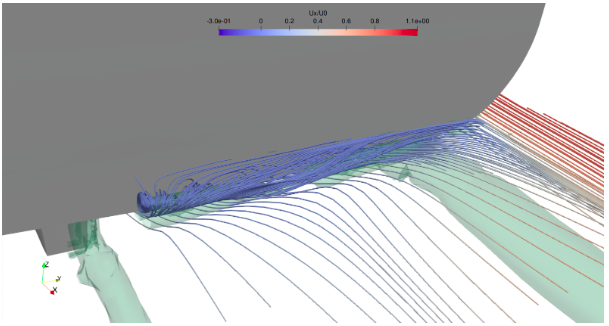
\includegraphics[width=\linewidth]{images/195-016-consup-modelo.png}
        \caption{Escala modelo, $Fr = 0{.}16$}
    \end{subfigure}
    \hfill
    \begin{subfigure}{0.48\textwidth}
        \centering
        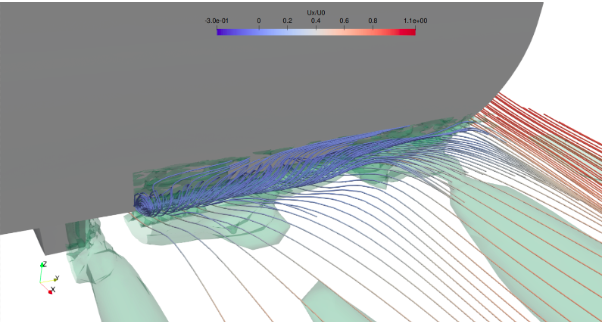
\includegraphics[width=\linewidth]{images/195-016-consup-real.png}
        \caption{Escala buque, $Fr = 0{.}16$}
    \end{subfigure}

    \vspace{0.5cm}

    \begin{subfigure}{0.48\textwidth}
        \centering
        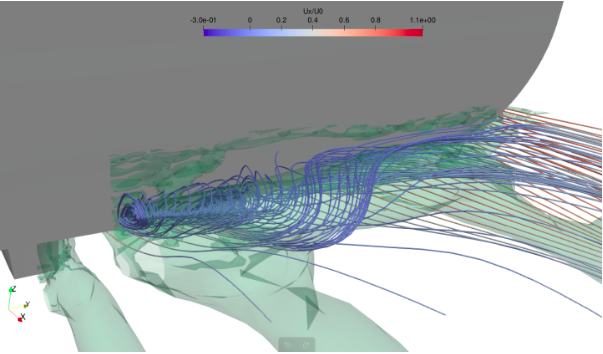
\includegraphics[width=\linewidth]{images/195-036-consup-modelo.png}
        \caption{Escala modelo, $Fr = 0{.}36$}
    \end{subfigure}
    \hfill
    \begin{subfigure}{0.48\textwidth}
        \centering
        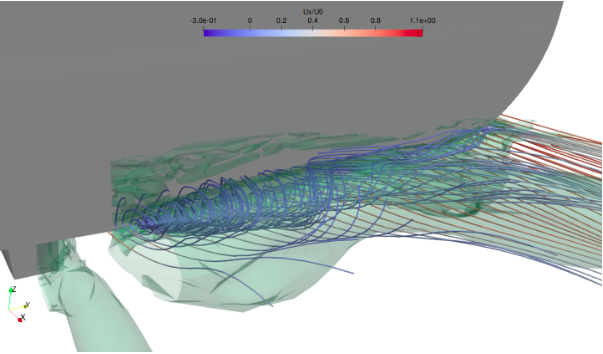
\includegraphics[width=\linewidth]{images/195-036-consup-real.png}
        \caption{Escala buque, $Fr = 0{.}36$}
    \end{subfigure}

    \caption{Comparación de la recirculación en popa sumergida para distintas 
    escalas y números de Froude (calado 0{.}195~m). Casos con superficie libre.}
    \label{fig:recirculacion_comparativa1}
\end{figure}

De manera análoga, en los casos de cuerpo doble ilustrados en la Figura~\ref{fig:recirculacion_comparativa2}, la estructura de recirculación es igualmente estable en todo el rango de velocidades y escalas analizadas. La similitud entre los resultados con y sin superficie libre, tanto a escala 
modelo como a escala buque, confirma que la hipótesis de doble cuerpo captura adecuadamente la física del flujo en la zona de popa para este casco. La persistencia de la recirculación al aumentar $Re$ es precisamente la 
condición que, según \citet{korkmaz_wetted_transom}, origina el déficit de resistencia viscosa en la extrapolación estándar y que motiva la aplicación del método 2--$k$.

\begin{figure}[htpb]
    \centering
    \begin{subfigure}{0.48\textwidth}
        \centering
        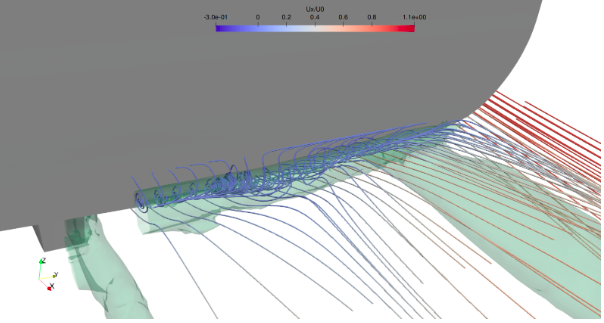
\includegraphics[width=\linewidth]{images/195-016-sinsup-modelo.png}
        \caption{Escala modelo, $Fr = 0{.}16$}
    \end{subfigure}
    \hfill
    \begin{subfigure}{0.48\textwidth}
        \centering
        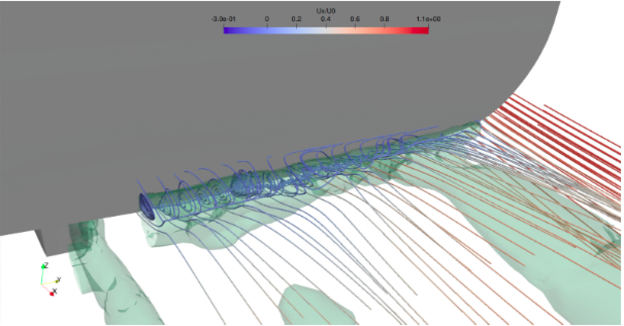
\includegraphics[width=\linewidth]{images/195-016-sinsup-real.png}
        \caption{Escala buque, $Fr = 0{.}16$}
    \end{subfigure}

    \vspace{0.5cm}

    \begin{subfigure}{0.48\textwidth}
        \centering
        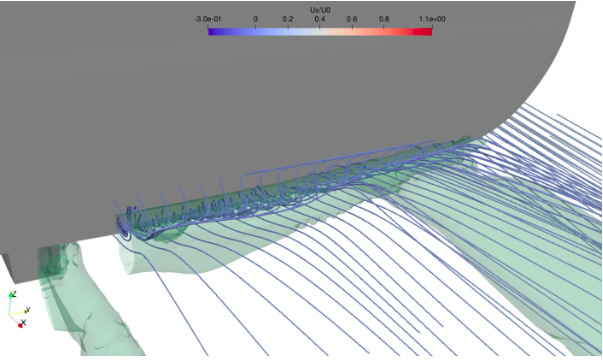
\includegraphics[width=\linewidth]{images/195-036-sinsup-modelo.png}
        \caption{Escala modelo, $Fr = 0{.}36$}
    \end{subfigure}
    \hfill
    \begin{subfigure}{0.48\textwidth}
        \centering
        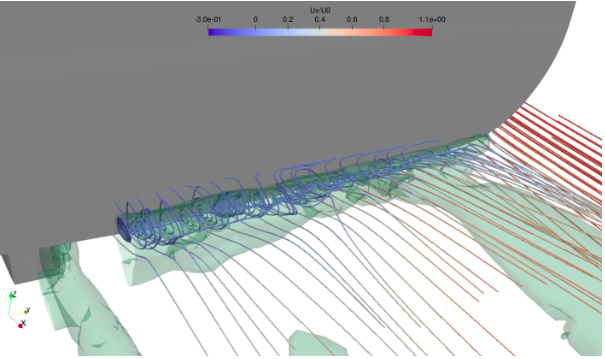
\includegraphics[width=\linewidth]{images/195-036-sinsup-real.png}
        \caption{Escala buque, $Fr = 0{.}36$}
    \end{subfigure}

    \caption{Comparación de la recirculación en popa sumergida para distintas 
    escalas y números de Froude (calado 0{.}195~m). Casos sin superficie libre.}
    \label{fig:recirculacion_comparativa2}
\end{figure}

\subsection{Aplicación al Pesquero~1}

La geometría de popa del Pesquero~1 presenta una inmersión del espejo que, según los criterios establecidos por \citet{korkmaz_wetted_transom}, debe evaluarse en condición estática ($Fr = 0$), ya que el método demanda los parámetros geométricos correspondientes al buque en reposo. La Tabla~\ref{tab:tpa_transom_params} resume los parámetros calculados para esa condición.

\begin{table}[h]
\centering
\caption{Parámetros de popa sumergida del \textit{P1} en condición estática 
($Fr = 0$, calado $T = 0{.}195$~m).}
\label{tab:tpa_transom_params}
\small
\begin{tabular}{lc}
\toprule
\textbf{Parámetro} & \textbf{Valor} \\
\midrule
$A_{tr}$ [m$^2$]            & 0{.}00222 \\
$A_{\max}$ [m$^2$]          & 0{.}04 \\
$y_{tr}$ [m]                & 0{.}198 \\
$T_{tr}$ [m]                & 0{.}0164 \\
$T$ [m]                     & 0{.}195 \\
\addlinespace[3pt]
$tr_{\text{ratio}}$         & 0{.}056 \\
$tr_{\text{fullness}}$      & 0{.}342 \\
\addlinespace[3pt]
$k_{tr}$                    & 0{.}025 \\
\bottomrule
\end{tabular}
\end{table}

El valor de $tr_{\text{ratio}} = 0{.}056$ supera el umbral de $0{.}025$ 
establecido por \citet{korkmaz_wetted_transom}, por lo que corresponde aplicar 
la corrección. El factor de forma de escala buque queda entonces:

\begin{equation}
    k_S = k_M + k_{tr} = 0{.}194 + 0{.}025 = 0{.}219
    \quad \Rightarrow \quad
    (1+k_S) = 1{.}219
\end{equation}

Sin embargo, para evaluar si este mecanismo explica la diferencia observada 
entre escalas, es necesario compararlo con la magnitud total de esa diferencia. 
Según los resultados de CFD DB presentados en la 
Sección~\ref{sec:analisis_efectos_escala}, el valor de $(1+k)$ a escala buque 
es de aproximadamente $1{.}716$ ($k_S = 0{.}716$), mientras que el valor adoptado 
a escala modelo es $(1+k_M) = 1{.}194$ ($k_M = 0{.}194$). La diferencia total es:

\begin{equation}
    k_S - k_M = 0{.}716 - 0{.}194 = 0{.}522
\end{equation}

La corrección de popa mojada $k_{tr} = 0{.}025$ representa apenas el $5\%$ de 
esa diferencia. El método 2--$k$ de \citet{korkmaz_wetted_transom} fue 
desarrollado para cascos donde la recirculación de popa espejo es el 
mecanismo dominante del efecto de escala en el factor de forma; en el 
\textit{P1}, en cambio, la diferencia entre escalas está gobernada por la 
evolución de $C_{PV}$ asociada a las estructuras vorticosas de quilla y 
pantoque, cuya intensidad se mantiene estable con $Re$, como se demostró en 
la Sección~\ref{sec:descomposicion_de_la_res_viscosa}. La recirculación de 
popa espejo contribuye a ese efecto de escala total, pero con un peso 
marginal.

\subsection{Conclusiones parciales}

El análisis comparativo de flujo confirma que la estructura de recirculación en la zona del espejo de popa se mantiene estable frente al cambio de escala, tanto en las simulaciones con superficie libre como en las de doble cuerpo. 
Esta persistencia de la recirculación con $Re$ es precisamente la condición que, según \citet{korkmaz_wetted_transom}, origina un déficit de resistencia viscosa en la extrapolación estándar y que justifica la aplicación del método 2--$k$.

La aplicación del método al \textit{P1} arroja $k_{tr} = 0{.}025$, lo que representa aproximadamente el $5\%$ de la diferencia total observada entre el factor de forma a escala modelo y a escala buque ($k_S - k_M = 0{.}522$). 
Este resultado permite cuantificar la contribución de la popa espejo sumergida al efecto de escala total y, al mismo tiempo, descartarla como causa principal: la diferencia predominante tiene su origen en la evolución de $C_{PV}$ asociada a las estructuras vorticosas de quilla y pantoque, cuyo mecanismo fue analizado en la Sección~\ref{sec:descomposicion_de_la_res_viscosa}. 
El análisis del efecto de la línea de fricción, que completa el diagnóstico de los efectos de escala en el \textit{P1}, se presenta en la Sección~\ref{sec:linea_de_friccion}.

\section{Efecto de la línea de fricción}\label{sec:linea_de_friccion}

Como se discutió en la Sección~\ref{sec:ITTC57}, el uso de la línea de 
correlación ITTC-57 introduce una dependencia artificial del factor de forma 
con el número de Reynolds que desaparece casi por completo al sustituirla 
por líneas de fricción numéricas (NFL), al menos para cascos de esbeltez 
moderada. En esta sección se evalúa si este efecto es suficiente para 
explicar la variación de $(1+k)$ con $Re$ observada en el \textit{P1}.

La Figura~\ref{ittc_nfl} presenta la variación de $(1+k)$ frente al número 
de Reynolds para el \textit{P1}, considerando la línea ITTC-57 
\citep{ITTC_resistance} y la NFL propuesta por \citet{Korkmaz2019NumericalFL}.

\begin{figure}[htpb]
	\centering
	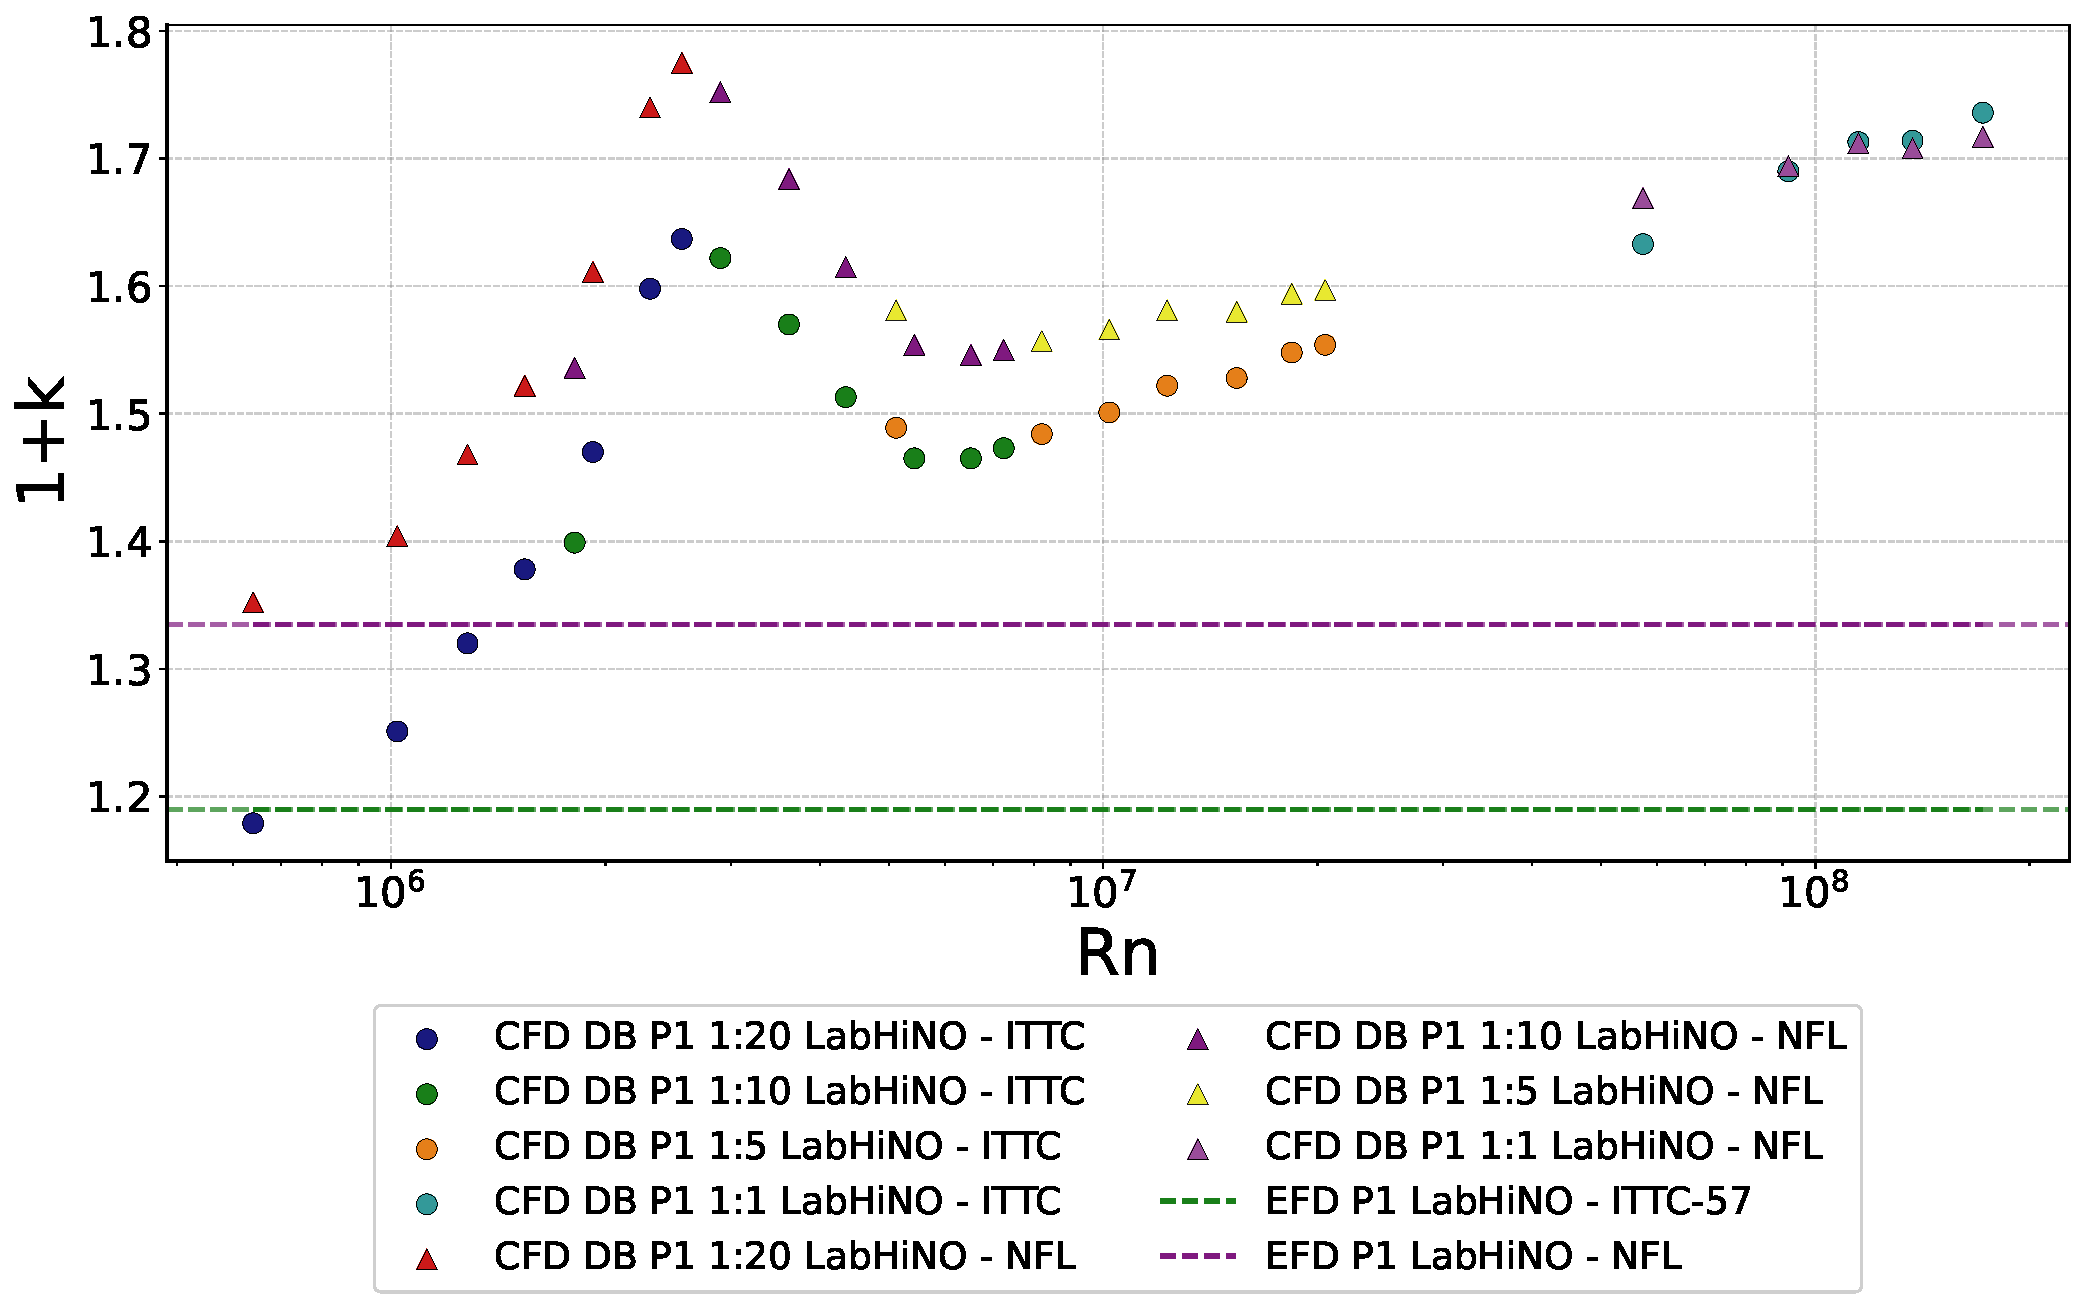
\includegraphics[width=.6\columnwidth]{images/ittc-nfl.pdf}
	\caption{Variación de $(1+k)$ en función de $Re$ para el \textit{P1} 
	empleando la línea ITTC-57 y la NFL de \citet{Korkmaz2019NumericalFL}.}
	\label{ittc_nfl}
\end{figure}

Al emplear la NFL, se observan valores de $(1+k)$ ligeramente más altos a 
bajos $Re$ y, en consecuencia, una variación total algo menor del factor de 
forma a lo largo del rango de escalas. Sin embargo, la diferencia entre el 
valor de $(1+k)$ a bajo y alto $Re$ continúa siendo considerable, del orden 
del 25\%, frente al 40\% obtenido con la ITTC-57. Para altos números de 
Reynolds (escala buque), el valor de $(1+k)$ resulta prácticamente idéntico 
independientemente de la línea de fricción utilizada, como cabría esperar 
dado que las diferencias entre formulaciones se concentran en el régimen de 
bajo $Re$.

En síntesis, la sustitución de la línea ITTC-57 por una NFL reduce 
parcialmente la variación de $(1+k)$ con $Re$, pero no la elimina: la 
diferencia entre escalas continúa siendo sustancial. Esto confirma que el 
efecto de escala en el \textit{P1} no puede atribuirse exclusivamente al 
sesgo de la línea de correlación, sino que responde principalmente a la 
física del flujo, en particular a la evolución de $C_{PV}$ con $Re$ 
asociada a las estructuras vorticosas de popa, como se analizó en la 
Sección~\ref{sec:descomposicion_de_la_res_viscosa}.

\section{Efecto de los modelos de turbulencia}

\subsection{Introducción y motivación del estudio}

El modelado de la turbulencia constituye una de las principales fuentes de 
incertidumbre en la simulación numérica de la resistencia viscosa. Los modelos 
basados en las ecuaciones de Navier--Stokes promediadas por Reynolds (RANS) 
introducen un cierre empírico a través de la denominada \textit{viscosidad 
turbulenta}, cuyo valor depende del modelo de turbulencia seleccionado. Dado 
que la estimación del factor de forma $(1+k)$ se basa en la partición entre 
resistencia friccional y de presión viscosa, cualquier variación en la 
predicción del campo de velocidades o en la distribución de esfuerzos de corte 
puede modificar significativamente el resultado final.

En esta sección se analiza la influencia del modelo de turbulencia sobre la 
determinación numérica del factor de forma, comparando cuatro formulaciones 
ampliamente utilizadas en hidrodinámica naval: $k$--$\omega$, $k$--$\omega$ SST, 
$k$--$\varepsilon$ estándar y $k$--$\varepsilon$ realizable. El objetivo es 
evaluar su sensibilidad en la estimación de $C_F$, $C_{PV}$ y $(1+k)$ para el 
caso del \textit{P1}, y verificar la consistencia de las predicciones frente al 
valor experimental obtenido mediante el método de Prohaska.

\subsection{Metodología y configuración numérica}

Las simulaciones se realizaron bajo las mismas condiciones numéricas y de 
contorno descritas en la Sección~\ref{sec:doble_cuerpo}: dominio de cuerpo 
doble sin superficie libre, flujo estacionario y configuración de malla 
equivalente. Las únicas variaciones entre casos corresponden al modelo de 
turbulencia empleado, de modo que las diferencias observadas sean atribuibles 
exclusivamente al cierre turbulento.

\subsection{Modelos de turbulencia analizados}

A continuación se presenta la formulación y las diferencias conceptuales entre 
los modelos de turbulencia empleados para el análisis de sensibilidad. El 
objetivo es contrastar el modelo $k$--$\omega$ SST, utilizado en todos los 
cálculos presentados hasta ahora, con formulaciones alternativas para evaluar 
su impacto en la predicción de la resistencia viscosa y el factor de forma 
$(1+k)$.

\paragraph{Modelo $k$--$\omega$ SST}

El modelo $k$--$\omega$ SST (\textit{Shear Stress Transport}) fue utilizado 
como modelo de referencia para todos los cálculos presentados en los capítulos 
anteriores. Su formulación detallada y la justificación de su elección se 
encuentran descritas en la Sección~\ref{sec:metodo_SST} del 
Capítulo~\ref{chap:Metodologia}. En esta comparativa, sus resultados sirven 
como línea de referencia frente a la cual se evalúan las desviaciones de los 
otros modelos.

\paragraph{Modelo $k$--$\omega$ estándar}

El modelo $k$--$\omega$ original \citep{Wilcox1988} es un modelo RANS de dos 
ecuaciones que resuelve la energía cinética turbulenta $k$ y la tasa 
específica de disipación $\omega$. Las ecuaciones de transporte se escriben 
como:

\begin{equation}
\frac{\partial k}{\partial t} + U_j \frac{\partial k}{\partial x_j}
=
P_k - \beta^* k \omega
+ \frac{\partial}{\partial x_j}
\left[
(\nu + \sigma_k \nu_t)\frac{\partial k}{\partial x_j}
\right],
\end{equation}

\begin{equation}
\frac{\partial \omega}{\partial t} + U_j \frac{\partial \omega}{\partial x_j}
=
\alpha \frac{\omega}{k} P_k - \beta \omega^2
+ \frac{\partial}{\partial x_j}
\left[
(\nu + \sigma_\omega \nu_t)\frac{\partial \omega}{\partial x_j}
\right],
\end{equation}

donde $U_j$ es la velocidad, $P_k$ es el término de producción de energía 
cinética turbulenta, $\nu$ es la viscosidad cinemática molecular, $\nu_t$ es la viscosidad cinemática turbulenta, y $\beta^*$, $\beta$, $\alpha$, 
$\sigma_k$ y $\sigma_\omega$ son constantes del modelo.

La viscosidad turbulenta se define como:

\begin{equation}
\nu_t = \frac{k}{\omega}.
\end{equation}

Aunque este modelo presenta una buena resolución de la capa límite viscosa 
sin necesidad de funciones de amortiguamiento, es conocido por su fuerte 
sensibilidad a las condiciones de contorno de turbulencia en el flujo libre 
(\textit{freestream sensitivity}), lo que puede afectar la predicción del 
campo turbulento global si el dominio no es suficientemente grande.

\paragraph{Modelo $k$--$\varepsilon$ estándar}

El modelo $k$--$\varepsilon$ estándar \citep{Launder1974} resuelve las 
ecuaciones de transporte para la energía cinética turbulenta $k$ y su tasa 
de disipación $\varepsilon$:

\begin{equation}
\frac{\partial k}{\partial t} + U_j \frac{\partial k}{\partial x_j}
=
P_k - \varepsilon
+ \frac{\partial}{\partial x_j}
\left[
(\nu + \sigma_k \nu_t)\frac{\partial k}{\partial x_j}
\right],
\end{equation}

\begin{equation}
\frac{\partial \varepsilon}{\partial t} + U_j \frac{\partial \varepsilon}{\partial x_j}
=
C_{\varepsilon 1} \frac{\varepsilon}{k} P_k
- C_{\varepsilon 2} \frac{\varepsilon^2}{k}
+ \frac{\partial}{\partial x_j}
\left[
(\nu + \sigma_\varepsilon \nu_t)\frac{\partial \varepsilon}{\partial x_j}
\right],
\end{equation}

donde $C_{\varepsilon 1}$, $C_{\varepsilon 2}$ y $\sigma_\varepsilon$ son 
constantes del modelo. La viscosidad turbulenta se define como:

\begin{equation}
\nu_t = C_\mu \frac{k^2}{\varepsilon},
\end{equation}

con $C_\mu$ constante. Este modelo asume equilibrio local entre producción y 
disipación y fue calibrado para flujos completamente turbulentos y alejados 
de la pared. Como consecuencia, tiende a sobreestimar la difusión turbulenta 
en la capa límite y no resulta adecuado para capturar con precisión efectos 
de separación bajo gradientes de presión adversos, tendiendo a predecir una 
re-adhesión del flujo demasiado temprana en la popa.

\paragraph{Modelo $k$--$\varepsilon$ realizable}

El modelo $k$--$\varepsilon$ realizable \citep{Shih1994} introduce 
modificaciones conceptuales al modelo estándar con el objetivo de cumplir 
restricciones matemáticas sobre los esfuerzos de Reynolds 
(\textit{realizability}), evitando la generación de energía cinética negativa 
en flujos con grandes deformaciones medias. En particular, el coeficiente 
$C_\mu$ deja de ser constante y pasa a depender del estado local del flujo 
(tasa de deformación y rotación), y la ecuación de $\varepsilon$ se 
reformula para mejorar la predicción de flujos con rotación, separación 
moderada y estelas:

\begin{equation}
\nu_t = C_\mu(\mathbf{U}, \nabla \mathbf{U}) \frac{k^2}{\varepsilon},
\end{equation}

donde $\mathbf{U}$ es el vector de velocidades medias y $\nabla \mathbf{U}$ 
su gradiente. Estas modificaciones permiten reducir la difusión excesiva 
característica del modelo estándar y mejorar la predicción de estructuras 
vorticosas coherentes. Se incluye en este análisis para evaluar si una 
formulación $k$--$\varepsilon$ mejorada puede acercarse a los resultados del 
modelo $k$--$\omega$ SST para la determinación del factor de forma.

\subsection{Comparación de resistencia viscosa}

La Figura~\ref{fig:comparacion_cd} presenta los coeficientes de resistencia 
viscosa total $C_V$ obtenidos para los cuatro modelos de turbulencia en 
función del número de Reynolds. A bajo $Re$, donde el flujo se encuentra en 
régimen transicional, se observa una dispersión significativa entre modelos.

Entre los modelos evaluados, el $k$--$\omega$ SST predice los valores más 
bajos de $C_V$, mientras que el $k$--$\varepsilon$ estándar predice los 
valores más altos. El modelo $k$--$\varepsilon$ realizable reduce parcialmente 
esta discrepancia, situándose entre ambos. Este comportamiento coincide con 
lo reportado por \citet{Karim}, quien observó una secuencia análoga en la 
predicción de la resistencia de cuerpos sumergidos a $Re = 2\times10^7$: la 
mayor concordancia con los datos experimentales correspondió al $k$--$\omega$ 
SST, seguido del $k$--$\varepsilon$ realizable, el $k$--$\varepsilon$ estándar 
y finalmente el $k$--$\omega$.

A medida que $Re$ aumenta, las diferencias entre modelos disminuyen y todos 
convergen hacia una tendencia común. Esto sugiere que las discrepancias son 
dominantes solo en el rango transicional, donde la fracción de flujo laminar 
o la intensidad del campo de recirculación varían según el modelo.

\begin{figure}[htpb]
    \centering
    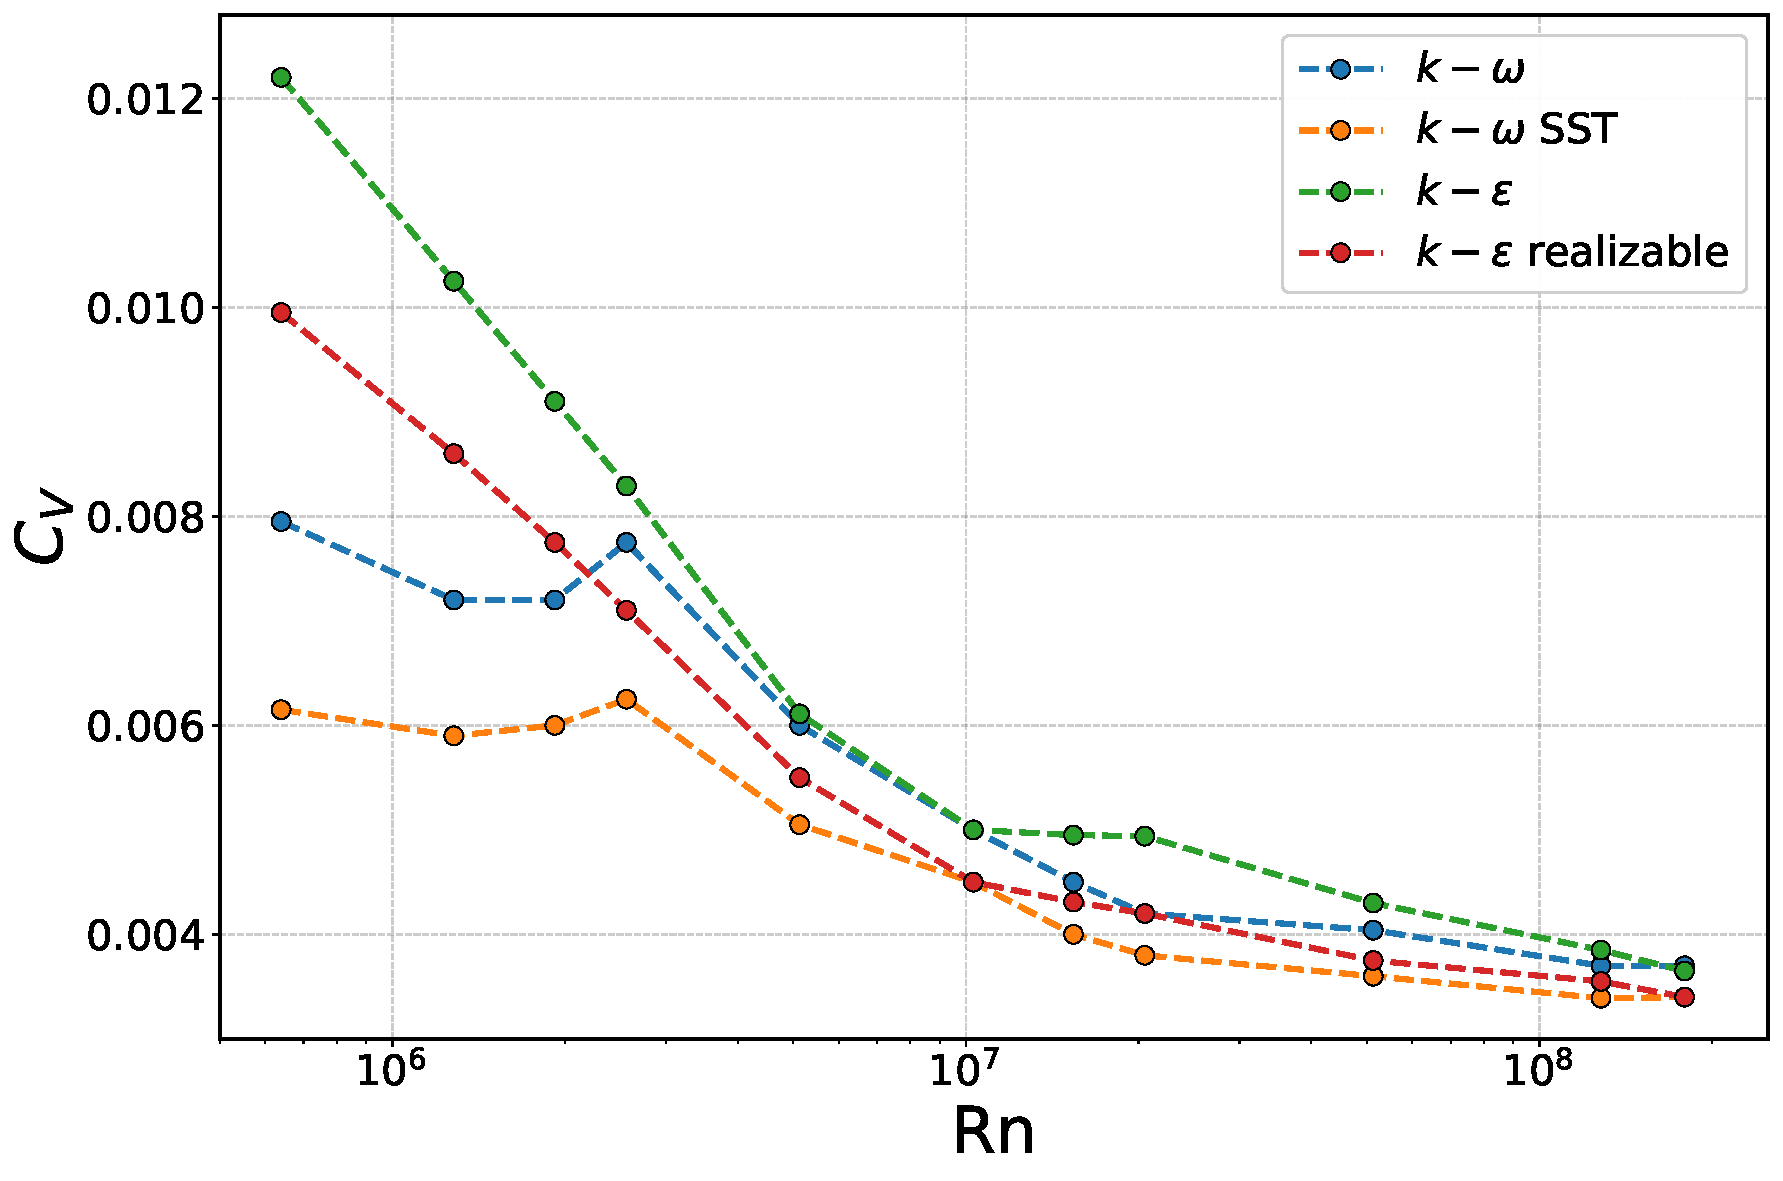
\includegraphics[width=0.75\textwidth]{images/comparacion_ct.pdf}
    \caption{Comparación de $C_V$ obtenido mediante distintos modelos de 
    turbulencia para el \textit{P1}.}
    \label{fig:comparacion_cd}
\end{figure}

\subsection{Efecto sobre el factor de forma}

La Figura~\ref{fig:comparacion_k} muestra la evolución del factor de forma 
$(1+k)$ con el número de Reynolds para los cuatro modelos. El $k$--$\omega$ 
SST presenta la mayor concordancia con el valor experimental del 
\textit{P1} ($1+k \approx 1.30$ en $Re \approx 10^6$). El modelo 
$k$--$\omega$ predice valores más altos de $(1+k)$ que el $k$--$\omega$ SST 
en el rango intermedio ($Re \approx 2\times10^7$), atribuibles al incremento 
de la resistencia de presión viscosa observada en ese régimen. En cambio, el 
$k$--$\varepsilon$ estándar y el $k$--$\varepsilon$ realizable exhiben 
pendientes más suaves y tienden a converger hacia valores similares a los del 
$k$--$\omega$ SST a alto $Re$.

\begin{figure}[htpb]
    \centering
    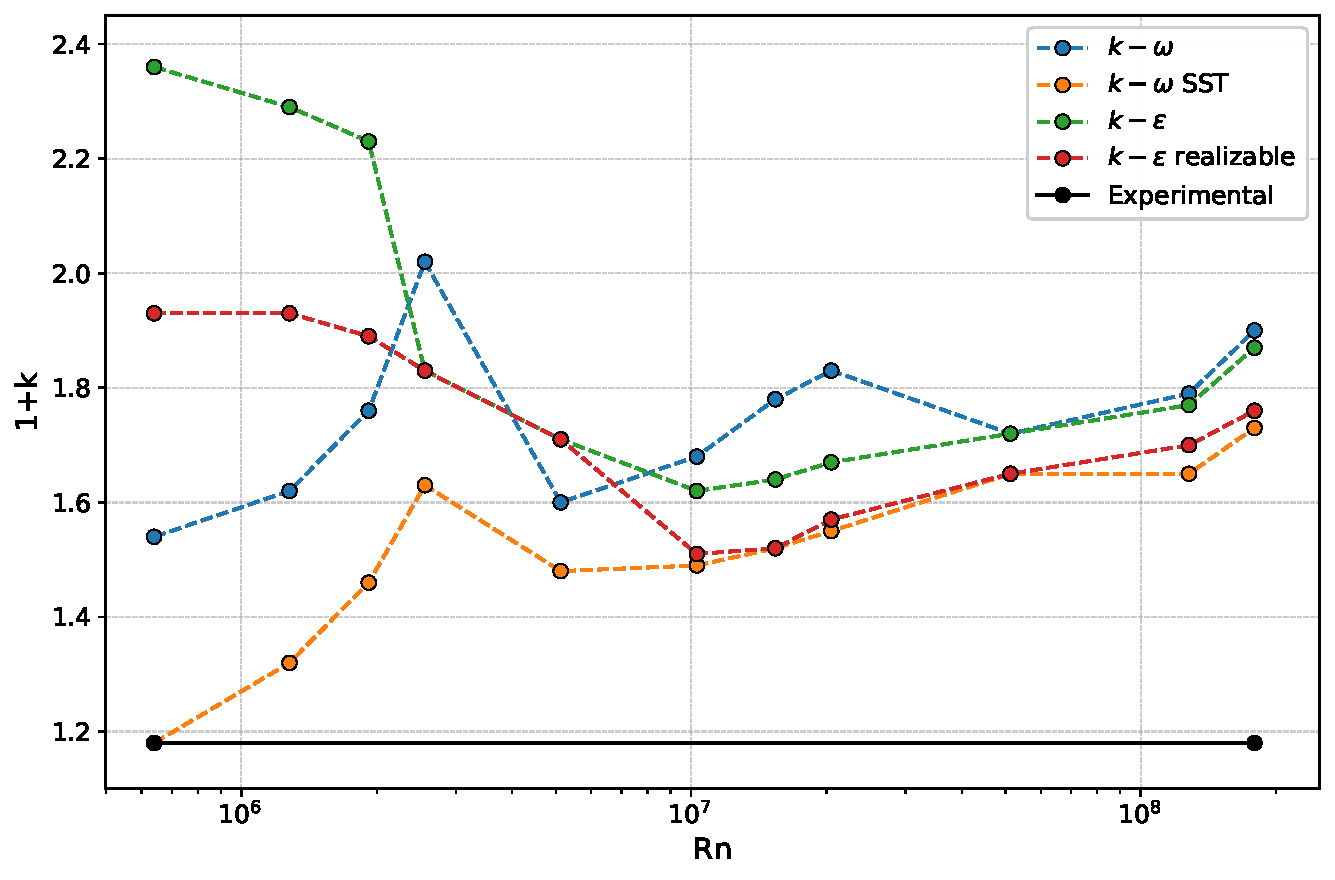
\includegraphics[width=0.75\textwidth]{images/comparacion_k.pdf}
    \caption{Evolución del factor de forma $(1+k)$ en función de $Re$ para 
    distintos modelos de turbulencia. \textit{P1}.}
    \label{fig:comparacion_k}
\end{figure}

Este resultado pone de manifiesto que la elección del modelo de turbulencia 
afecta principalmente el comportamiento del factor de forma a bajo y mediano 
$Re$, donde el flujo puede contener zonas parcialmente laminares o 
recirculaciones locales en popa. A alto $Re$, donde el flujo es plenamente 
turbulento y las capas límite están bien desarrolladas, la sensibilidad del 
cálculo a la elección del modelo disminuye marcadamente.

\subsection{Descomposición de la resistencia según origen friccional y 
de presión viscosa}

Para profundizar en las causas de las diferencias anteriores, las 
Figuras~\ref{fig:comparacion_cf} y \ref{fig:comparacion_cp} muestran la 
variación del coeficiente de fricción $C_F$ y del coeficiente de presión 
viscosa $C_{PV}$ con $Re$. En la primera se aprecia que $k$--$\omega$ SST 
reproduce la correlación ITTC-57 en casi todo el rango de $Re$, salvo en la 
zona más baja donde el flujo se encuentra parcialmente transicional. Por su 
parte, el $k$--$\omega$ tiende a sobreestimar $C_F$, lo que explica los 
mayores valores de $C_V$ y $(1+k)$ obtenidos anteriormente.

El análisis del coeficiente de presión viscosa revela diferencias menores 
entre modelos, pero con tendencias sistemáticas: el $k$--$\omega$ y el 
$k$--$\varepsilon$ estándar predicen valores de $C_{PV}$ ligeramente 
superiores a los del $k$--$\omega$ SST, mientras que el $k$--$\varepsilon$ 
realizable se sitúa entre ambos. Estas diferencias se resumen 
cuantitativamente en la Figura~\ref{fig:dif_pp}, donde se presentan las 
variaciones porcentuales de $C_F$ y $C_{PV}$ respecto de $k$--$\omega$ SST.

\begin{figure}[htpb]
    \centering
    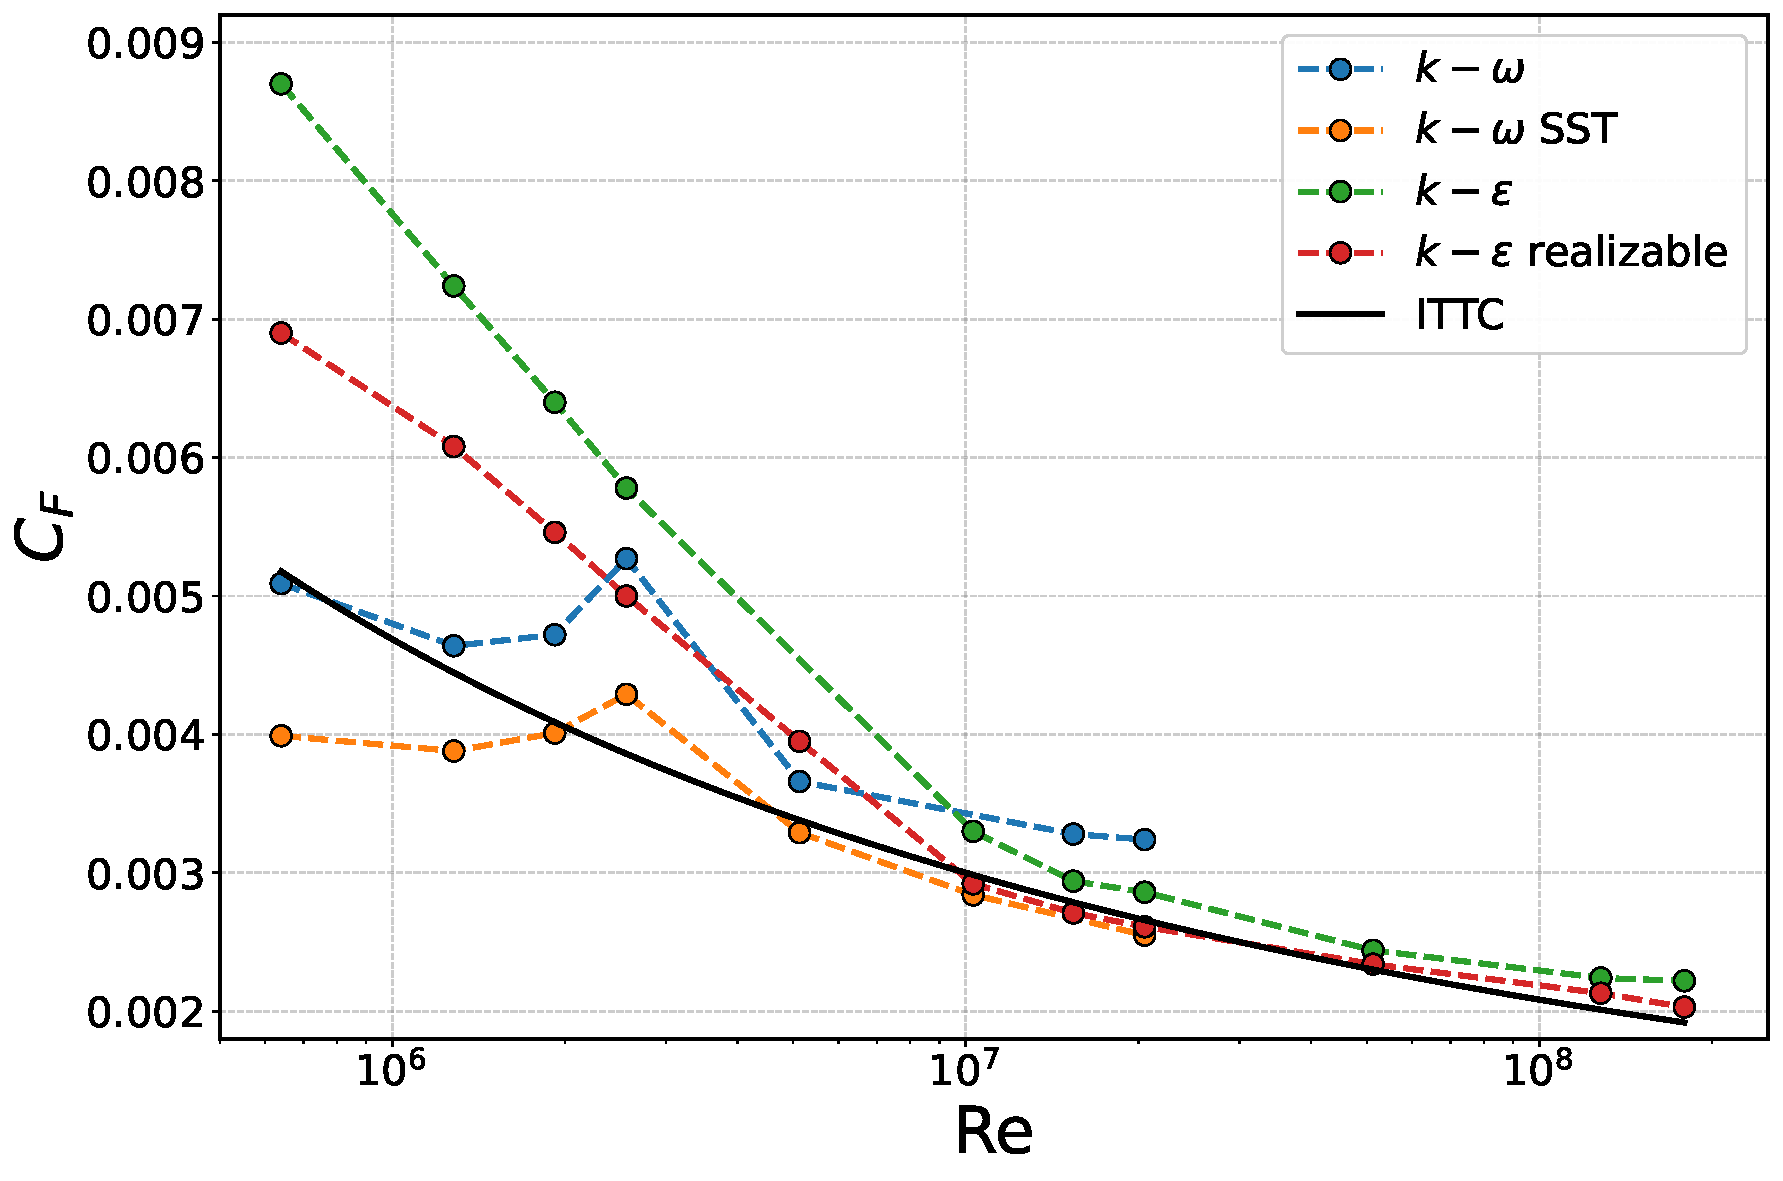
\includegraphics[width=0.75\textwidth]{images/comparacion_cf.pdf}
    \caption{Coeficiente de fricción $C_F$ en función del número de Reynolds 
    para distintos modelos de turbulencia. \textit{P1}.}
    \label{fig:comparacion_cf}
\end{figure}

\begin{figure}[htpb]
    \centering
    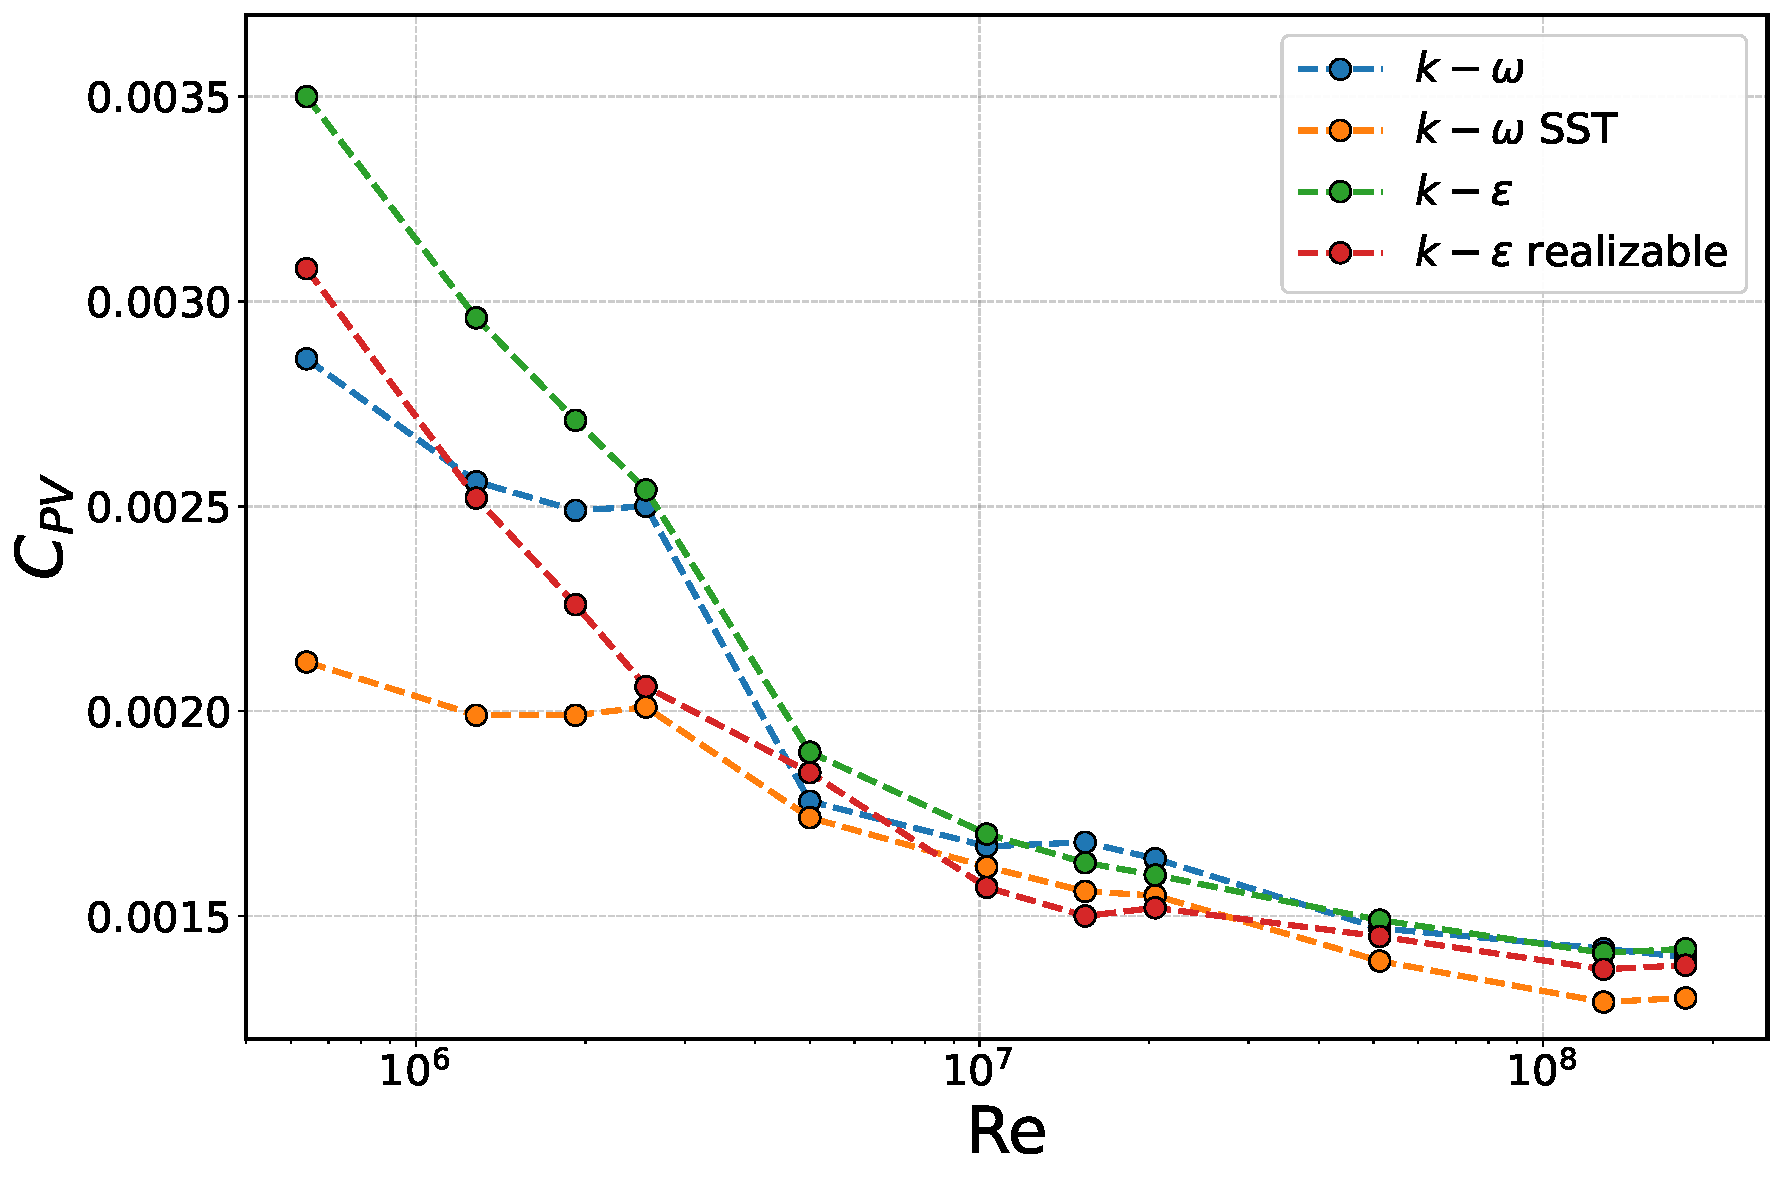
\includegraphics[width=0.75\textwidth]{images/comparacion_cp.pdf}
    \caption{Coeficiente de presión viscosa $C_{PV}$ en función del número 
    de Reynolds para distintos modelos de turbulencia. \textit{P1}.}
    \label{fig:comparacion_cp}
\end{figure}

\begin{figure}[htpb]
    \centering
    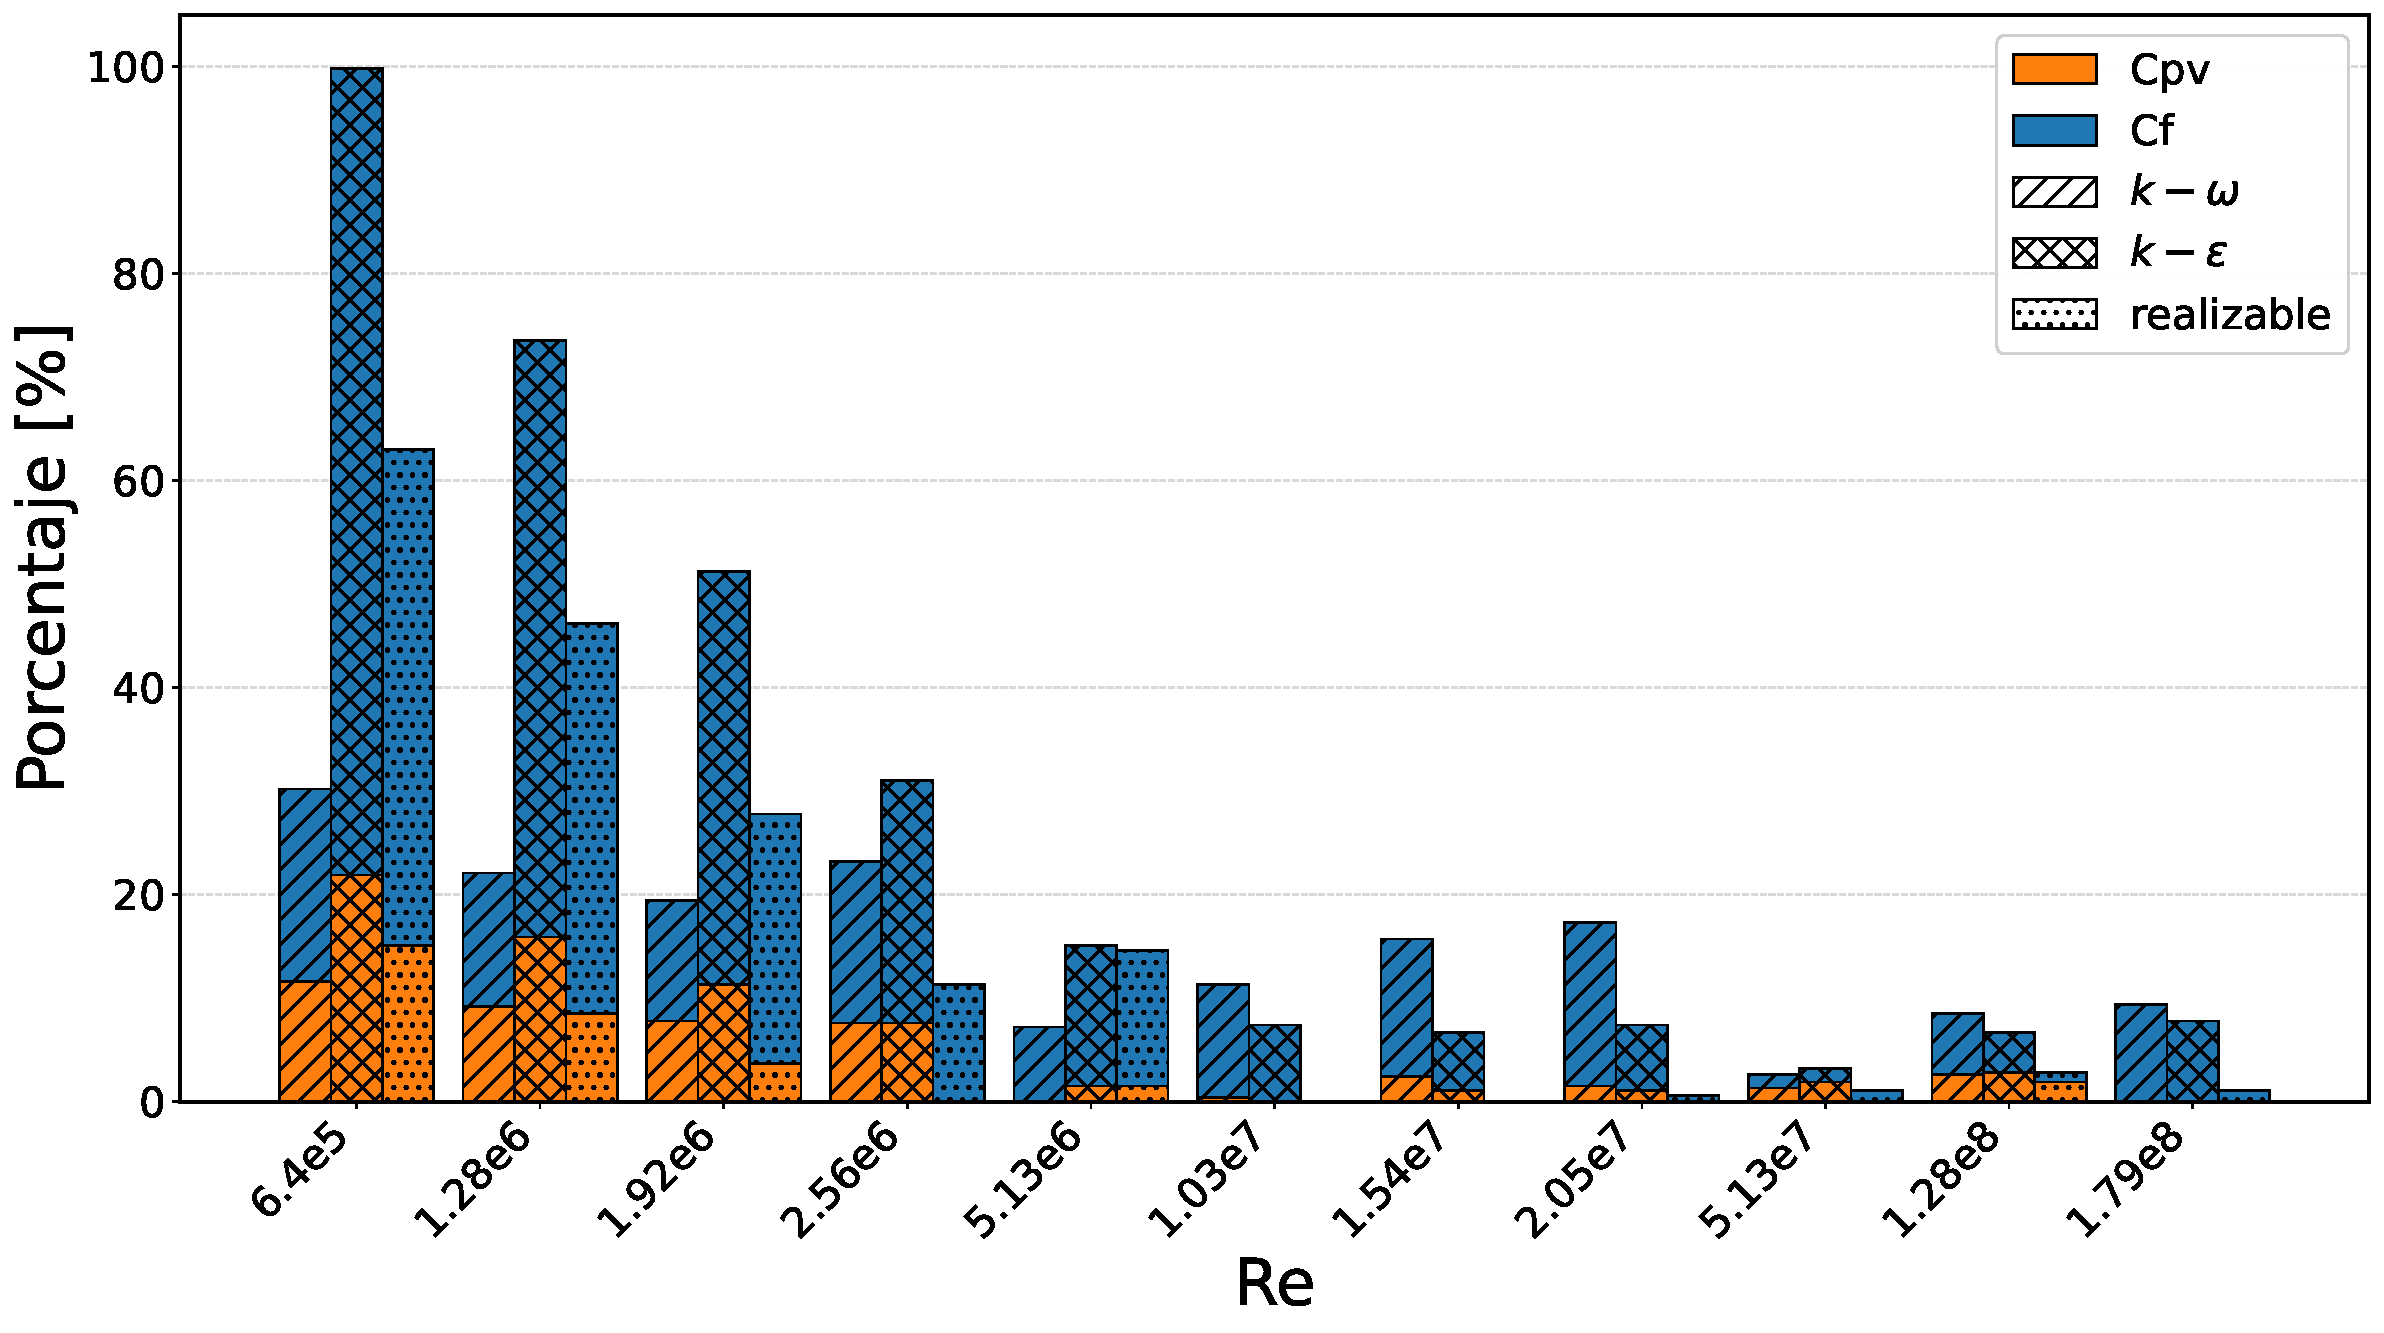
\includegraphics[width=0.85\textwidth]{images/dif_pp.pdf}
    \caption{Diferencia porcentual de $C_F$ y $C_{PV}$ respecto al modelo 
    $k$--$\omega$ SST.}
    \label{fig:dif_pp}
\end{figure}

Se observa que la mayor dispersión entre modelos ocurre a bajo $Re$, 
principalmente en la componente friccional. En ese régimen, una pequeña 
variación en $C_F$ repercute fuertemente en la estimación de $(1+k)$, dado 
que la resistencia por fricción representa la mayor parte de la resistencia 
viscosa. A medida que aumenta $Re$ y el flujo se torna plenamente turbulento, las predicciones de $C_F$ convergen a la línea ITTC-57 y la diferencia entre modelos se reduce notablemente. En cambio, $C_{PV}$ mantiene una tendencia creciente más suave con $Re$, y sus diferencias relativas entre modelos son menores pero más persistentes, lo que explica parte de la dispersión residual en el factor de forma a gran escala.

\subsection{Recomendaciones para la selección de modelos en estudios de escala}

Para estudios CFD orientados a la determinación del factor de forma mediante
extrapolación de resistencia viscosa, los resultados obtenidos permiten
formular las siguientes recomendaciones prácticas:

\begin{itemize}
    \item Priorizar modelos capaces de resolver adecuadamente la región cercana a la pared en régimen transicional, como el $k$--$\omega$ SST, 
    cuya formulación híbrida ofrece un comportamiento estable tanto en la capa límite como en el flujo externo.
    \item Mantener una resolución de malla coherente con el modelo seleccionado, especialmente en términos de $y^+$.
    \item Evaluar explícitamente la sensibilidad del factor de forma al modelo de turbulencia cuando se trabaja a bajos $Re$, en particular 
    antes de emplear $(1+k)$ como base para extrapolaciones a escala buque.
    \item Aplicar los modelos $k$--$\varepsilon$ con cautela en regímenes transicionales, dado que su mayor sensibilidad paramétrica puede 
    conducir a una sobreestimación del efecto viscoso global.
\end{itemize}

\subsection{Conclusiones parciales}

El análisis realizado permite caracterizar la influencia del modelo de turbulencia sobre la estimación de $(1+k)$ en función del régimen de flujo.
A bajos números de Reynolds, las diferencias entre modelos son significativas y afectan tanto $C_F$ como $C_{PV}$, amplificando su impacto en el valor
final del factor de forma. A medida que el flujo evoluciona hacia un régimen plenamente turbulento, esta sensibilidad se atenúa y las predicciones
convergen progresivamente.

En particular, los modelos $k$--$\varepsilon$ tienden a sobreestimar $(1+k)$ en el rango transicional, mientras que el $k$--$\omega$ SST presenta una
evolución más moderada y mejor alineada con el valor experimental. Esto confirma que la correcta interpretación del factor de forma en CFD requiere
considerar explícitamente el régimen de flujo y el modelo de turbulencia empleado, especialmente cuando los resultados se utilizan como base para
extrapolaciones o comparaciones con datos experimentales.

\section{Efecto de la relación de aspecto L/B}

\subsection{Motivación y observaciones sobre L/B en cascos de baja esbeltez}

Como se demostró en las Secciones~\ref{sec:analisis_efectos_escala} 
y~\ref{sec:descomposicion_de_la_res_viscosa}, los métodos tradicionales 
de extrapolación de resistencia, ampliamente validados para buques 
mercantes esbeltos, asumen que el factor de forma $(1+k)$ tiende a 
estabilizarse conforme aumenta el número de Reynolds. Sin embargo, este 
supuesto no se cumple para el \textit{P1}, donde las estructuras 
vorticosas longitudinales desprendidas de la quilla y el pantoque generan 
estelas más anchas y pérdidas viscosas por presión que persisten hasta la 
escala buque, impidiendo la estabilización de $(1+k)$ dentro del rango 
analizado.

En esta sección se mostrará la incapacidad de los métodos empíricos para la estimación del factor de forma en el \textit{P1} y luego se extenderá el análisis al Pesquero 2 y 3, que cuentan con distintas razones $L/B$, para identificar tendencias generalizables.

\subsection{Análisis CFD y comparación de presión y resistencia viscosa}

El comportamiento del coeficiente de presión viscosa $C_{PV}$ resulta 
determinante para comprender la evolución del factor de forma $(1+k)$ con el 
número de Reynolds. Esto se observó claramente al comparar el \textit{P1} con 
el KCS, como fue presentado en la Figura~\ref{cpv_friccion}. Si bien $C_{PV}$ 
disminuye con $Re$ de manera similar en ambos cascos en términos absolutos, 
la proporción que $C_{PV}$ representa dentro de $C_V$ es sustancialmente 
mayor en el \textit{P1} que en el KCS a lo largo de todo el rango de escalas 
analizado.

Esta diferencia responde a la dificultad del flujo para recuperar la presión 
en la popa del \textit{P1}, donde se generan grandes estructuras vorticosas 
que persisten aun a escala buque. En el KCS, $C_F$ domina ampliamente sobre 
$C_{PV}$, de modo que $(1+k) = C_V/C_{F0}$ queda gobernado por el 
comportamiento de $C_F$, que sigue de cerca a $C_{F0}$ y produce un cociente 
prácticamente constante. En el \textit{P1}, en cambio, $C_F$ y $C_{PV}$ son 
de magnitud comparable, y la caída más lenta de $C_{PV}$ respecto a $C_{F0}$ 
impide que el cociente se estabilice dentro del rango de escalas analizado.

Al comparar el valor de $(1+k)$ obtenido para el \textit{P1} con 
correlaciones empíricas desarrolladas para buques mercantes, surge una 
doble inconsistencia. Por un lado, el valor de $(1+k) \approx 1{.}73$ 
obtenido por CFD DB a escala buque no tiene precedente en la literatura 
de hidrodinámica naval: no se ha encontrado un valor comparable para 
ningún casco desnudo documentado hasta la fecha. Por otro lado, las 
fórmulas empíricas consideradas fueron desarrolladas a partir de ensayos 
con buques mercantes de esbeltez convencional. Entre los parámetros 
geométricos de entrada de estas correlaciones ($C_B$, $L/B$, $B/T$, 
$S/L^2$, $L/\nabla^{1/3}$), la relación $L/B = 3{.}75$ del \textit{P1} 
resulta notablemente inferior a la de los buques mercantes típicos para 
los cuales fueron calibradas, lo que compromete la aplicabilidad de estas 
expresiones a este tipo de casco. Como consecuencia, las fórmulas 
disponibles no reproducen los altos valores observados mediante CFD DB 
para escala buque. La Tabla~\ref{tab:empiricos} presenta las expresiones 
utilizadas y los valores obtenidos para el \textit{P1}, y la 
Figura~\ref{empiricos} ilustra la alta dispersión entre correlaciones y 
la falta de coincidencia con los resultados numéricos y experimentales.

\begin{table}[htpb]
\centering
\caption{Correlaciones empíricas para la estimación del factor de forma 
$(1+k)$ y valores obtenidos para el \textit{P1} 
($L = 34{.}8$~m, $B = 9{.}28$~m, $T = 3{.}9$~m, 
$S = 449{.}6$~m$^2$, $C_B = 0{.}64$, $\nabla = 152{.}0$~m$^3$).}
\label{tab:empiricos}
\small
\begin{tabularx}{\textwidth}{lXc}
\toprule
\textbf{Método} & \textbf{Expresión} & \boldmath{$(1+k)$} \\
\midrule
\citet{molland2017ship} (Watanabe) &
$\displaystyle 1 + k = 1 - 0{.}095 + 
\frac{25{.}6\,C_B}{(L/B)^2\,\sqrt{B/T}}$ &
$1{.}660$ \\[10pt]

\citet{conn1968results} &
$\displaystyle 1 + k = 1 + 18{.}7
\left(\frac{C_B\,B}{L}\right)^{2}$ &
$1{.}545$ \\[10pt]

\citet{grigson2000planar} &
$\displaystyle 1 + k = 1 + 0{.}028 + 3{.}3\,
\frac{S}{L^2}\sqrt{\frac{C_B\,B}{L}}$ &
$1{.}534$ \\[10pt]

\citet{wright1984viscous} &
$\displaystyle 1 + k = 2{.}48\,
C_B^{0{.}1526}\,
\left(\frac{B}{T}\right)^{0{.}0533}\,
\left(\frac{B}{L}\right)^{0{.}3856}$ &
$1{.}457$ \\[10pt]

\citet{couser1997calm} &
$\displaystyle 1 + k = 2{.}76\,
\left(\frac{L}{\nabla^{1/3}}\right)^{-0{.}4}$ &
$1{.}616$ \\[10pt]

Prohaska (EFD, presente trabajo) & --- & $1{.}19$ \\
\bottomrule
\end{tabularx}
\end{table}

\begin{figure}[htpb]
    \centering
    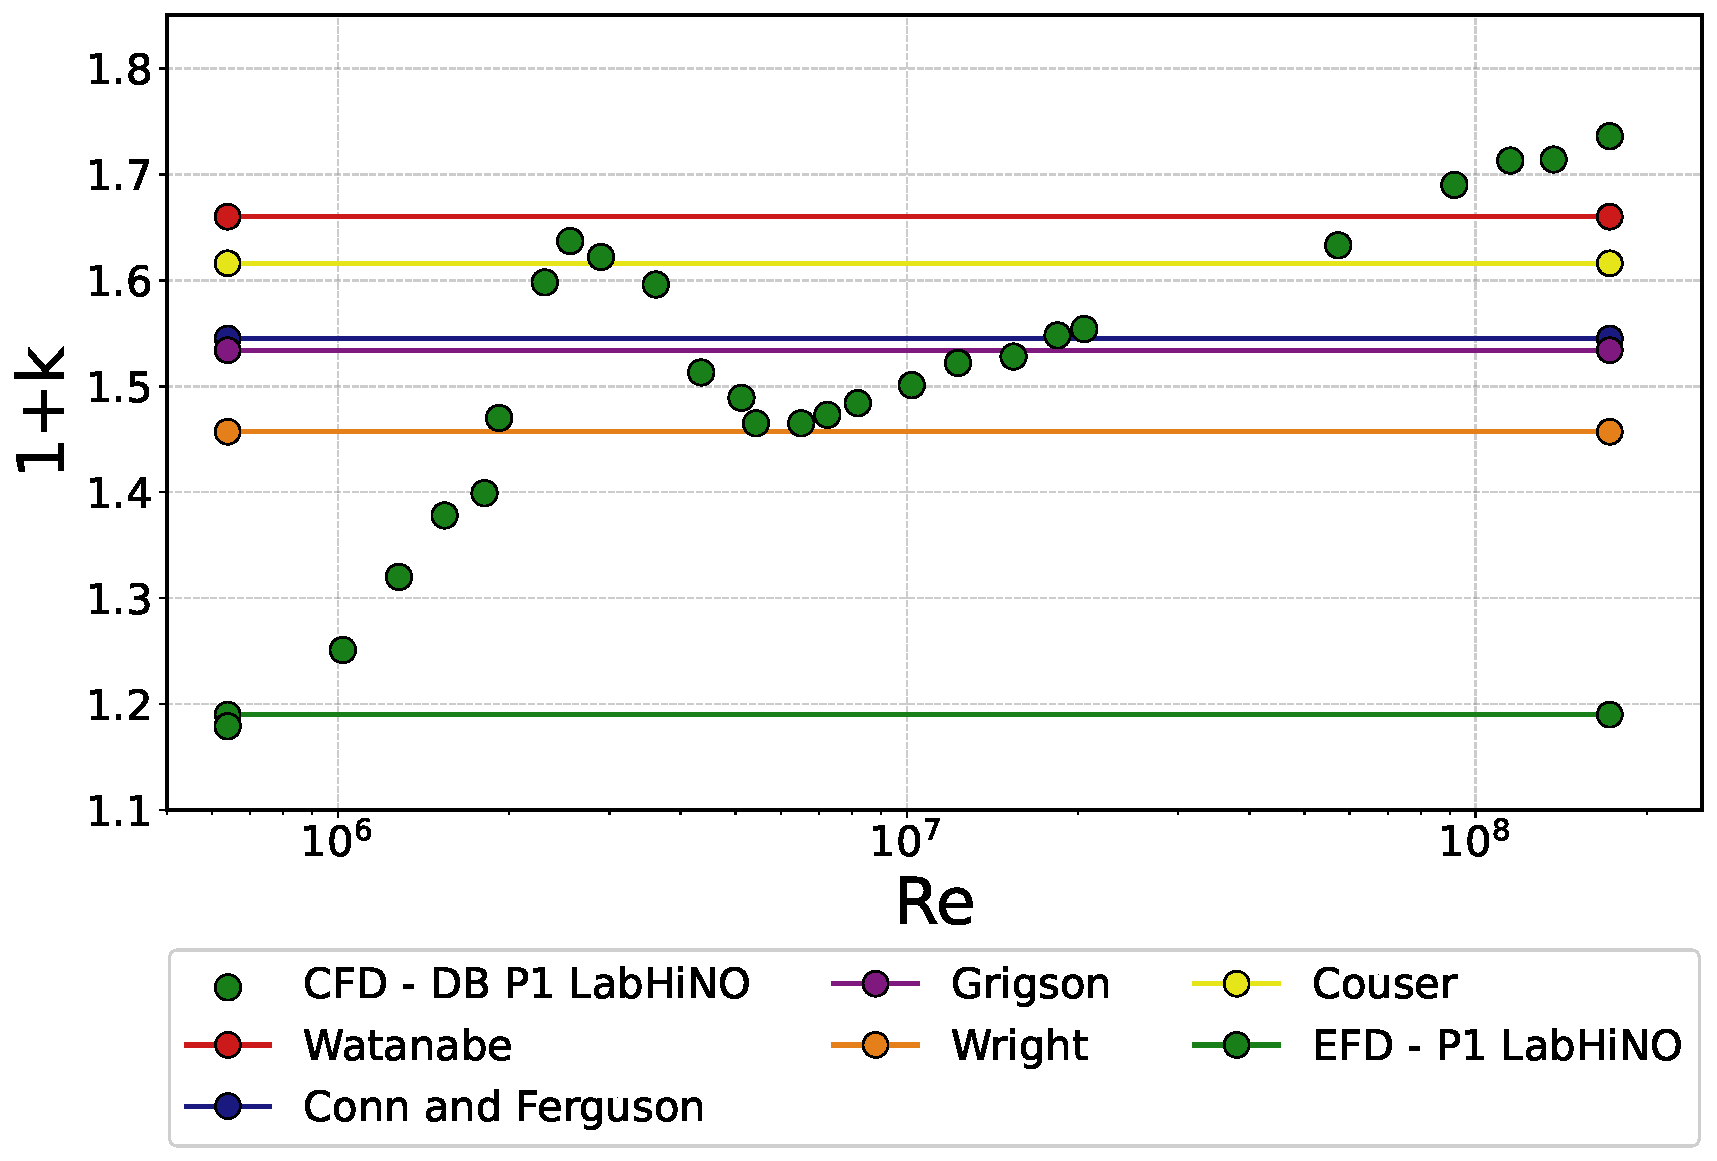
\includegraphics[width=.6\textwidth]{./images/empiricos.pdf}
    \caption{Valores de $(1+k)$ para el \textit{P1} en función de $Re$, 
    obtenidos por CFD DB, EFD y correlaciones empíricas de la literatura 
    \citep{molland2017ship, conn1968results, grigson2000planar, 
    wright1984viscous, couser1997calm}.}
    \label{empiricos}
\end{figure}

Estas dos observaciones en conjunto, la ausencia de valores comparables 
en la literatura naval y la inaplicabilidad de las correlaciones 
existentes, motivaron la búsqueda de referencias en otros ámbitos donde 
la geometría controla la resistencia viscosa y donde se manejan cuerpos 
de baja esbeltez. En aerodinámica, el método clásico de estimación de 
resistencia de fuselajes consiste en multiplicar el coeficiente de 
fricción turbulenta de placa plana por un factor de forma empírico 
dependiente de la razón de esbeltez del cuerpo, y por el área mojada. 
El fuselaje se modela como un cuerpo de revolución, y el parámetro 
geométrico principal es la razón de esbeltez $l/d$, directamente análoga 
a $L/B$ en cascos de buques. \citet{hoerner1965drag} fue el primero en 
derivar un factor de forma para cuerpos de revolución a partir de 
correlaciones con ensayos en túnel de viento, obteniendo una curva válida 
para $l/d > 4.5$ que fue extrapolada hacia valores menores sin validación 
experimental. Autores posteriores \citep{raymer2019aircraft, 
torenbeek2010synthesis, roskam1987airplane, shevell1989fundamentals} 
continuaron ajustando estas correlaciones para extender su rango de 
validez hacia cuerpos menos esbeltos. La Figura~\ref{aerodynamics} 
superpone estas correlaciones con los valores de $(1+k)$ a escala buque 
obtenidos por CFD DB para el \textit{P1} ($L/B = 3.53$) y para el KCS 
($L/B = 7.14$, datos de \citet{TerzievDataSet}), representados en 
función de $l/d = L/B$.

La Tabla~\ref{tab:aerodinamicos} presenta las expresiones de las 
correlaciones aerodinámicas consideradas en la Figura~\ref{aerodynamics}.

\begin{table}[htpb]
\centering
\caption{Correlaciones aerodinámicas de factor de forma para cuerpos de 
revolución en función de la razón de esbeltez $l/d$.}
\label{tab:aerodinamicos}
\small
\begin{tabularx}{\textwidth}{lX}
\toprule
\textbf{Método} & \textbf{Expresión} \\
\midrule
\citet{hoerner1965drag} &
$\displaystyle \mathrm{FF} = 1 + 
\frac{1{.}5}{(l/d)^{1{.}5}} + 
\frac{7}{(l/d)^{3}}$ \\[10pt]

\citet{torenbeek2010synthesis} &
$\displaystyle \mathrm{FF} = 1 + 
\frac{2{.}2}{(l/d)^{1{.}5}} + 
\frac{3{.}8}{(l/d)^{3}}$ \\[10pt]

\citet{shevell1989fundamentals} &
$\displaystyle \mathrm{FF} = 2{.}939 - 0{.}7666\,\frac{l}{d} + 
0{.}1328\left(\frac{l}{d}\right)^{2}
- 0{.}01074\left(\frac{l}{d}\right)^{3}
+ 3{.}275\times10^{-4}\left(\frac{l}{d}\right)^{4}$ \\[10pt]

\citet{raymer2019aircraft} (Raymer new) &
$\displaystyle \mathrm{FF} = 0{.}9 + 0{.}0025\,\frac{l}{d} + 
\frac{5}{(l/d)^{1{.}5}}$ \\[10pt]

\citet{roskam1987airplane} &
$\displaystyle \mathrm{FF} = 1 + 0{.}0025\,\frac{l}{d} + 
\frac{60}{(l/d)^{3}}$ \\
\bottomrule
\end{tabularx}
\end{table}

\begin{figure}[htpb]
    \centering
    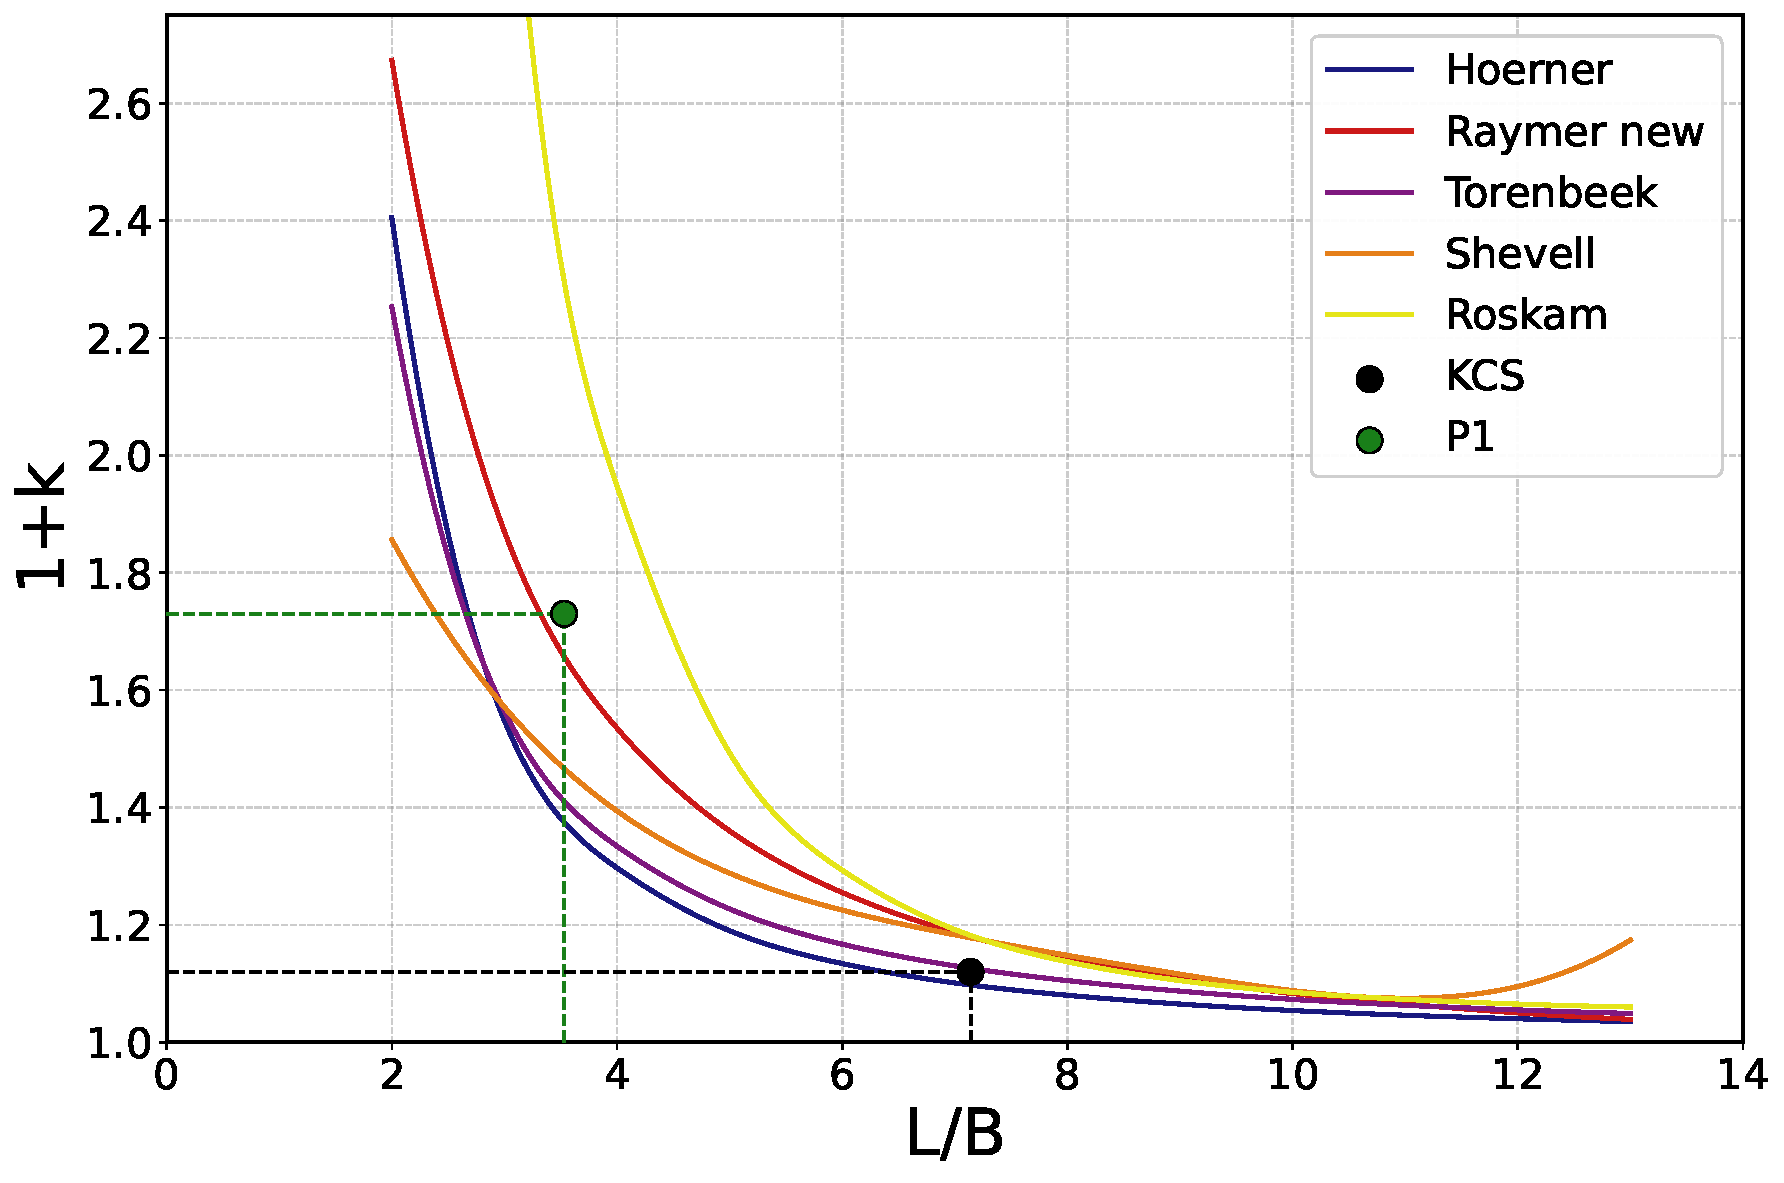
\includegraphics[width=.6\textwidth]{./images/aerodynamics.pdf}
    \caption{Factores de forma para cuerpos de revolución en función de la 
    razón de esbeltez $l/d$ y comparación con valores CFD DB para el 
    \textit{P1} y el KCS. Datos de \citep{hoerner1965drag, 
    raymer2019aircraft, torenbeek2010synthesis, roskam1987airplane, 
    shevell1989fundamentals, TerzievDataSet}.}
    \label{aerodynamics}
\end{figure}

El valor del KCS coincide con la curva de \citet{hoerner1965drag}, coherente 
con su alta esbeltez y con el rango para el que dicha curva fue derivada 
originalmente. El valor del \textit{P1}, en cambio, muestra mayor afinidad 
con la curva ``Raymer New'' \citep{raymer2019aircraft}, ajustada 
específicamente para cuerpos de menor esbeltez. Es notable que correlaciones 
provenientes de un campo de estudio diferente, pero que incluyen valores de 
$l/d$ suficientemente bajos como para abarcar la geometría del \textit{P1}, 
reproduzcan los resultados CFD con mayor fidelidad que las correlaciones 
navales tradicionales.

Este hallazgo sugiere que, para cascos con baja razón $L/B$, las 
correlaciones aerodinámicas representan mejor la dependencia geométrica del 
factor de forma que las correlaciones navales tradicionales, desarrolladas 
para valores de $L/B$ significativamente más altos.


\subsection{Presentación de pesqueros con distintos L/B}

Los tres pesqueros analizados en esta tesis, presentados en la 
Sección~\ref{sec:presentacion_modelos} junto con el KCS, fueron 
seleccionados precisamente por cubrir un rango de relaciones de esbeltez 
$L/B$ distintas: $3{.}53$ (\textit{P1}), $3{.}23$ (\textit{P2}) y 
$2{.}85$ (\textit{P3}). Esta diversidad geométrica permite evaluar de 
manera sistemática si el comportamiento observado para el \textit{P1} 
constituye un caso aislado o refleja una tendencia estructural asociada 
a la baja esbeltez. La Figura~\ref{fig:LB_comparisson} presenta las 
cuatro geometrías escaladas a la misma eslora, con el fin de resaltar 
las diferencias morfológicas asociadas al ancho relativo, volumen 
transversal y forma de popa.

\begin{figure}[h!]
    \centering
    % --- Primera columna: nombres ---
    \begin{subfigure}{.18\textwidth}
        \centering
        \vspace{1em}
        \footnotesize % controla el tamaño de texto
        \textbf{KCS (L/B = 7.12)}\\[3em]
        \textbf{Fishing Vessel 1 (L/B = 3.53)}\\[3.5em]
        \textbf{Fishing Vessel 2 (L/B = 3.23)}\\[3.5em]
        \textbf{Fishing Vessel 3 (L/B = 2.85)}
        \caption*{ }
    \end{subfigure}
    % --- Segunda columna: vista frontal ---
    \begin{subfigure}{.15\textwidth}
        \centering
        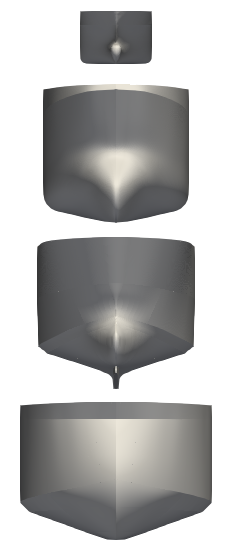
\includegraphics[width=\linewidth]{./images/L-B-front.png}
        \caption{Front view}
    \end{subfigure}%
    % --- Tercera columna: vista lateral ---
    \begin{subfigure}{.395\textwidth}
        \centering
        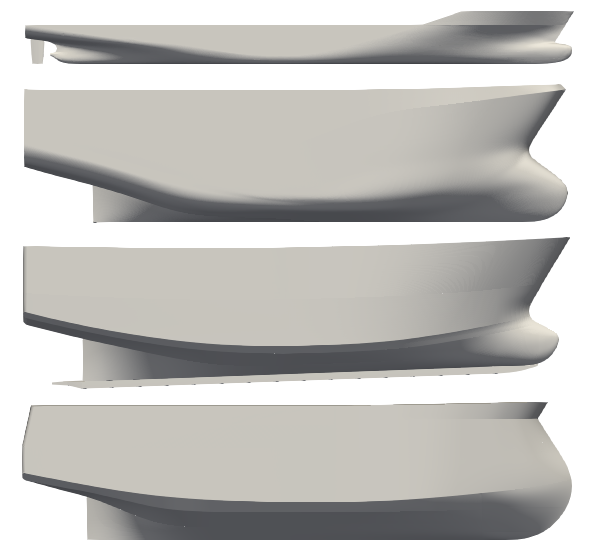
\includegraphics[width=\linewidth]{./images/L-B-side.png}
        \caption{Side view}
    \end{subfigure}
    \begin{subfigure}{.24\textwidth}
        \centering
        \vspace{1em}
        \footnotesize % controla el tamaño de texto
        \textbf{L = 230m , B = 32.2m \\ $\lambda$ = 1:79}\\[3em]
        \textbf{L = 34.79m , B = 9.28m \\ $\lambda$ = 1:20 }\\[3.5em]
        \textbf{L = 27.6m , B = 7.8m \\ $\lambda$ = 1:10}\\[3.5em]
        \textbf{L= 22.3m , B = 7.8m \\ $\lambda$ = 1:13}
        \caption*{ }
    \end{subfigure}
    \caption{Tested models. The four hulls are shown scaled to equal length for direct comparison.}
    \label{fig:LB_comparisson}
\end{figure}

Al disminuir $L/B$, las secciones transversales se vuelven más robustas y la transición hacia la popa más abrupta, lo que favorece la aparición de regiones extensas de presión adversa y el desprendimiento de estructuras vorticosas de gran escala. Estas características inducen mayores valores de $C_{PV}$ y explican la persistencia de la presión viscosa incluso a escala buque. A pesar de sus diferencias individuales, los tres pesqueros comparten proporciones y distribución volumétrica similares, lo que sugiere la presencia de un comportamiento hidrodinámico común asociado a la baja esbeltez.


\subsection{Generalización del comportamiento observado y formulación empírica}\label{sec:generalizacion_LB}

Como se mostró en la Figura~\ref{fig:Re_formfactor} de la 
Sección~\ref{sec:analisis_efectos_escala}, los tres pesqueros presentan 
un crecimiento continuo y no asintótico de $(1+k)$ incluso hacia escala 
buque, en marcado contraste con el KCS, que exhibe el incremento inicial 
y posterior estabilización esperados conforme se desarrolla la capa límite 
turbulenta.

La consistencia entre los tres modelos confirma que este comportamiento no es propio de un caso aislado, sino un rasgo estructural de cascos con $L/B < 4$. A medida que disminuye la esbeltez, aumenta el componente de presión viscosa y, en consecuencia, el factor de forma. La tendencia creciente y no asintótica en los pesqueros sugiere que la influencia de la presión viscosa domina su comportamiento hidrodinámico incluso en condiciones de escala buque.

Para interpretar esta dependencia geométrica, se recurrió nuevamente a correlaciones aerodinámicas desarrolladas para cuerpos de revolución, donde el factor de forma se expresa en función de la razón de esbeltez $l/d$. La Figura~\ref{fig:aero_comparison_full} incorpora simultáneamente las diferentes curvas aerodinámicas clásicas junto con los valores de $(1+k)$ provenientes de CFD DB para los cuatro cascos estudiados, todos representados en términos de $l/d = L/B$.

\begin{figure}[h]
    \centering
    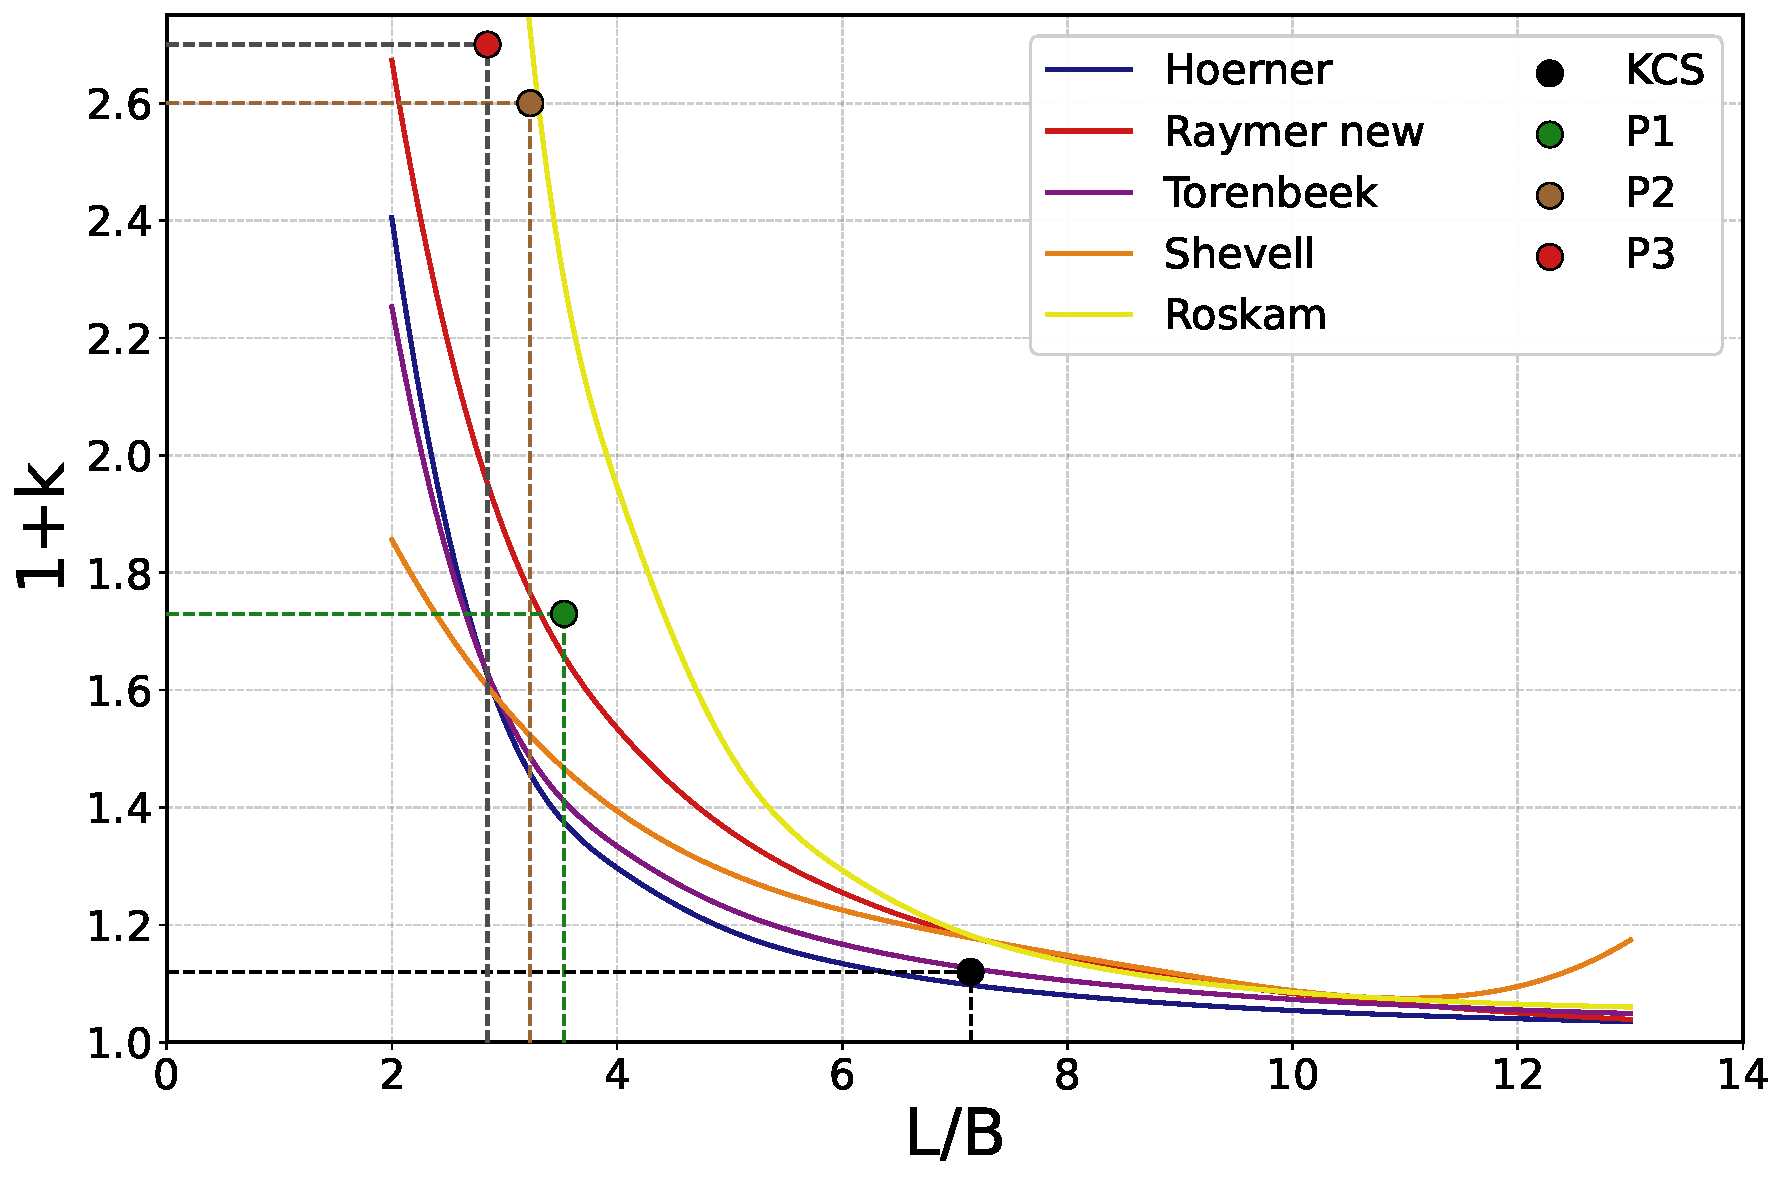
\includegraphics[width=.6\textwidth]{./images/aerodynamics2.pdf}
    \caption{Comparación entre correlaciones aerodinámicas de factor de forma y los valores $(1+k)$ obtenidos mediante CFD DB para los tres pesqueros y el KCS, representados en función de $l/d = L/B$.}
    \label{fig:aero_comparison_full}
\end{figure}

El gráfico revela una tendencia clara:  
\begin{itemize}
    \item El valor correspondiente al KCS se ubica en la región de altas esbelteces y coincide con la curva clásica de Hoerner, como era de esperar para un casco alargado.
    \item Los tres pesqueros, caracterizados por $L/B < 4$, se agrupan en la región de cuerpos poco esbeltos y exhiben proximidad a las correlaciones propuestas por \cite{roskam1987airplane} y \cite{raymer2019aircraft}.
    \item La alineación de los tres pesqueros refuerza la existencia de un mecanismo geométrico común que explica sus elevados valores de $(1+k)$.
\end{itemize}

Estos resultados sugieren que, para cascos de baja esbeltez, la relación entre $(1+k)$ y $L/B$ se comporta de manera análoga a la que se observa en cuerpos de revolución evaluados en aerodinámica. En consecuencia, la utilización directa de correlaciones aerodinámicas provee un marco más apropiado para interpretar la evolución del factor de forma en esta clase de buques que las fórmulas navales tradicionales, desarrolladas para valores significativamente más altos de $L/B$.

Este hallazgo abre la posibilidad de desarrollar una formulación empírica específica para pesqueros de baja esbeltez que permita predecir el comportamiento de $(1+k)$ a escala buque sin necesidad de extrapolar correlaciones que fueron diseñadas en base a buques considerablemente más esbeltos.


\subsection{Implicancias para el escalado y la extrapolación de resultados}

La marcada dependencia del factor de forma con el número de Reynolds, 
observada en los pesqueros analizados, tiene consecuencias directas sobre 
la extrapolación de resistencia y la estimación de la potencia efectiva a 
escala buque. En particular, los valores elevados de $(1+k)$ obtenidos para 
estos cascos, junto con su crecimiento sostenido hacia altas escalas, 
desafían el supuesto central del método ITTC: la igualdad entre los factores 
de forma del modelo y del buque ($k_{M} = k_{S}$).

Como se desarrolla en la Sección~\ref{sec:prediccion_potencia}, el 
procedimiento estándar de predicción de potencia \citep{ITTC_Performance_prediction} 
estima la resistencia total del buque como:
%
\begin{equation}
    C_{TS} = (1 + k_S)\,C_{FS0} + C_W + \Delta C_F + C_A
\end{equation}
%
donde $C_{FS0}$ es el coeficiente de fricción del buque calculado mediante 
la línea ITTC-57, $C_W$ es el coeficiente de resistencia por formación de 
olas obtenido del modelo físico como residuo de la descomposición viscosa, 
y $\Delta C_F$ y $C_A$ corresponden a las correcciones por rugosidad y 
correlación recomendadas por la ITTC. Este método supone que $k_S = k_M$, 
es decir, que el factor de forma es independiente de la escala.

Sin embargo, los resultados CFD DB demostraron que este supuesto no se 
cumple para los pesqueros estudiados. El fuerte incremento de $(1+k)$ con 
$Re$ implica que:
%
\begin{equation}
    k_S \gg k_M,
\end{equation}
%
lo que significa que la extrapolación tradicional subestima sistemáticamente 
la resistencia viscosa del buque y, por ende, la potencia efectiva necesaria.

La resistencia total del buque a escala buque y la potencia efectiva se 
obtienen como (Sección~\ref{sec:prediccion_potencia}):
%
\begin{equation}
    R_{TS} = \tfrac{1}{2}\,\rho\,V_S^2\,S_S\,C_{TS}
\end{equation}
%
\begin{equation}
    P_{ES} = R_{TS}\,V_S
\end{equation}
%
donde $\rho$ es la densidad del agua, $V_S$ la velocidad del buque y $S_S$ 
la superficie mojada a escala buque.

Para cuantificar la magnitud del error introducido por la selección de un valor inapropiado de $k$, se compararon tres enfoques (Tablas~\ref{tbl:metodos_abs} y \ref{tbl:metodos_delta}):

\begin{itemize}
    \item \textbf{Método 1 (ITTC–EFD)}: $k_M = k_S$, obtenido por el método de Prohaska en modelo.
    \item \textbf{Método 2 (CFD–EFD, doble k)}: valores distintos de $k_M$ y $k_S$, determinados mediante CFD DB para modelo y buque. La idea es propuesta por \cite{korkmaz_wetted_transom} pero en su caso la diferencia nace exclusivamente de la popa sumergida, mientras que según la presente tesis la necesidad surge de los efectos de escala presentados en la Sección \ref{sec:descomposicion_de_la_res_viscosa} (Cpv).
    \item \textbf{Método 3 ($k = 0$)}: empleado cuando no es posible determinar el factor de forma ni experimentalmente ni mediante CFD; asume resistencia viscosa puramente friccional, equivalente a tratar el casco como una placa plana. Provee una cota de referencia para cuantificar el error asociado a ignorar completamente los efectos de forma.

\end{itemize}

\begin{table*}[htbp]
\caption{$C_{TS}$, $R_{TS}$ y $P_{ES}$ estimados mediante tres enfoques distintos para velocidades de operación del \textit{P1}.}

\label{tbl:metodos_abs}
\scriptsize
\centering

\begin{tabular}{c c c
    r r r
    r r r
    r r r}
\toprule
\multirow{2}{*}{$Fr$} &
\multicolumn{2}{c}{Velocidad} &
\multicolumn{3}{c}{Method 1 (EFD)} &
\multicolumn{3}{c}{Method 2 (EFD--CFD)} &
\multicolumn{3}{c}{Method 3 ($k=0$)} \\
\cmidrule(lr){2-3}
\cmidrule(lr){4-6}
\cmidrule(lr){7-9}
\cmidrule(lr){10-12}
 & $v_S$ & $v_S$ &
 $C_{TS}$ & $R_{TS}$ & $P_{ES}$ &
 $C_{TS}$ & $R_{TS}$ & $P_{ES}$ &
 $C_{TS}$ & $R_{TS}$ & $P_{ES}$ \\
 & {[m/s]} & {[kn]} &
 & {[kN]} & {[kW]} &
 & {[kN]} & {[kW]} &
 & {[kN]} & {[kW]} \\
\midrule
0.26 & 4.71 & 9.16
     & 6.28 & 32.16 & 151.51
     & 7.33 & 37.53 & 176.79
     & 6.70 & 34.27 & 161.46 \\
0.30 & 5.34 & 10.38
     & 7.68 & 50.46 & 269.34
     & 8.71 & 57.22 & 305.45
     & 8.08 & 53.08 & 283.34 \\
\bottomrule
\end{tabular}
\end{table*}

\begin{table}[htbp]
\caption{Diferencias porcentuales en la potencia efectiva estimada respecto al método ITTC (Método 1).}
\label{tbl:metodos_delta}
\scriptsize
\centering

\begin{tabular}{c c c c c}
\toprule
$Fr$ & $v_S$ & $v_S$ & Method 2 vs 1 & Method 3 vs 1 \\
     & {[m/s]} & {[kn]} & {$\Delta P_{ES}$ [\%]} & {$\Delta P_{ES}$ [\%]} \\
\midrule
0.26 & 4.71 & 9.16  & 16.7 & 6.6 \\
0.30 & 5.34 & 10.38 & 13.4 & 5.2 \\
\bottomrule
\end{tabular}

\end{table}




Los resultados muestran que asumir $k=0$ (método 3) produce una sobreestimación de la potencia efectiva de aproximadamente $5\%$ respecto al método estándar ITTC. Como era de esperar, este método sobreestima la resistencia al ignorar la contribución viscosa de la forma del casco; sin embargo, su utilidad radica en que provee una referencia cuando no se dispone de ningún ensayo ni simulación para estimar el factor de forma, permitiendo acotar el error esperado.

En cambio, el método de doble $k$ basado en CFD DB (método 2) arroja una \textbf{potencia un 13–17$\%$ mayor} que la obtenida mediante el enfoque ITTC (método 1), diferencia atribuible al mayor valor de $k_S$ predicho numéricamente.

Estas discrepancias, del orden del 15$\%$ en términos de potencia instalada, son suficientemente significativas como para justificar una validación mediante pruebas de mar. Además, sugieren que las correlaciones empíricas introducidas en la Sección \ref{sec:generalizacion_LB}, originadas en aeronáutica y dependientes de la razón de esbeltez, podrían ser utilizadas como una estimación preliminar de $k_S$ de forma más confiable que las metodologías navales actuales. Esto permitiría implementar un método de extrapolación de doble $k$, donde $k_M$ se obtenga de CFD DB a escala modelo y $k_S$ de una correlación basada en $L/B$, evitando la necesidad de simulaciones CFD a escala buque.

El desarrollo de una curva específica de $(1+k)$ en función de $L/B$ para cascos pesqueros, particularmente para el rango $L/B < 4$, aparece por lo tanto como un paso clave para mejorar la predicción de resistencia y potencia efectiva en este tipo de buques.


\subsection{Conclusiones parciales}

La comparación con correlaciones empíricas desarrolladas para buques mercantes confirma la incapacidad de dichas formulaciones para reproducir los valores de $(1+k)$ obtenidos para el \textit{P1}, tanto a escala modelo como hacia escala buque. En contraste, las correlaciones aerodinámicas basadas en cuerpos de revolución muestran una correspondencia notable con los resultados CFD DB, ubicando al KCS y a los pesqueros en regiones coherentes con su respectiva esbeltez geométrica.

La incorporación de dos pesqueros adicionales con distintas relaciones $L/B$ refuerza esta observación: los tres cascos, pese a sus diferencias geométricas particulares, presentan un comportamiento hidrodinámico consistente, caracterizado por valores elevados y no asintóticos del factor de forma. Esta consistencia indica que la dependencia de $(1+k)$ con la relación de aspecto constituye un rasgo estructural de los cascos pesqueros de baja esbeltez y no una singularidad del \textit{P1}.

Finalmente, los resultados ponen de manifiesto que el supuesto fundamental del método ITTC (la igualdad entre los factores de forma del modelo y del buque) tiene incluso menor validez para este tipo de buques. Las diferencias observadas en la extrapolación de resistencia y potencia efectiva alcanzan magnitudes relevantes desde el punto de vista del diseño, lo que justifica la necesidad de enfoques alternativos. En este contexto, el uso combinado de CFD en configuración de doble cuerpo y correlaciones empíricas dependientes de $L/B$ emerge como una vía más consistente para la estimación del factor de forma en cascos pesqueros.
\chapter{Propulsión: efectos de escala en hélices en aguas abiertas} \label{chap:helices}
\mtcsettitle{minitoc}{Contenidos} 
\minitoc

\section{Introducción}
\label{sec:helices_intro}

El Capítulo~\ref{chap:antecedentes} presentó las limitaciones conocidas del procedimiento ITTC-78 para hélices: la hipótesis de que el efecto de escala es puramente friccional (Sección~\ref{sec:ittc78_propulsor}), la evidencia de una componente de presión no despreciable (Sección~\ref{sec:presion_escala}) y la posible presencia de un régimen de transición laminar-turbulenta a escala de modelo, con el consiguiente comportamiento no monótono de $K_T$ y $K_Q$ conocido como ``joroba'' (Sección~\ref{sec:chichon_antec}). Este capítulo cuantifica ambos mecanismos --distintos entre sí y que operan sobre saltos de Reynolds diferentes-- para dos hélices de referencia, combinando datos experimentales de archivo del LabHiNO y de terceros con simulaciones CFD RANS.

El primer mecanismo, que en adelante se denomina efecto de escala en régimen turbulento, es el cambio en la distribución de presión y fricción sobre la pala entre dos condiciones \emph{ambas} totalmente turbulentas, es decir, sin que intervenga la transición. Se caracteriza en las Secciones~\ref{sec:helices_validacion} y \ref{sec:helices_escala} mediante un barrido sistemático de diámetros de la hélice B4-60 de la serie Wageningen (de $D=0.14$ a $8.0$~m, a $J$ constante), resuelto con el modelo de turbulencia $k$-$\omega$ SST completamente turbulento. La Sección~\ref{sec:helices_validacion} valida primero la configuración numérica contra datos experimentales de archivo del LabHiNO y contra los polinomios de regresión de \citet{oosterveld1975}, y la Sección~\ref{sec:helices_escala} presenta el barrido de escala propiamente dicho, con la descomposición de $K_T$ y $K_Q$ en sus componentes de presión y fricción y la comparación directa con la predicción de la ITTC-78.

El segundo mecanismo, físicamente independiente del primero, es la presencia de un régimen de transición laminar-turbulenta sobre las palas dentro de la propia escala de modelo. Se aborda en la Sección~\ref{sec:helice_coreana} mediante una hélice de cuatro palas, de menor relación de áreas y con skew, ensayada en túnel de cavitación para cinco números de Reynolds de cuerda distintos. Los resultados muestran una protuberancia no monótona en $K_T$ y $K_Q$ en función del número de Reynolds --la joroba transicional introducida en la Sección~\ref{sec:chichon_antec}--, que el modelo totalmente turbulento no puede reproducir en ningún caso y que un modelo de transición ($\gamma$-$\widetilde{Re}_{\theta t}$, \citealp{langtry2009}), calibrado en la intensidad de turbulencia del disco y verificado en dos solvers independientes (OpenFOAM y StarCCM+), reproduce solo parcialmente. Esta sección evalúa además, mediante una simulación adicional a escala mayor, cómo se propaga esa dependencia del $Re_c$ de ensayo a través del procedimiento ITTC-78, y compara la fracción de presión obtenida para esta hélice con la de la B4-60 y con la reportada en la literatura para una geometría similar.

Ambas líneas de trabajo comparten el mismo punto ciego del procedimiento estándar --suponer que el efecto de escala es puramente friccional-- pero involucran fenómenos físicos distintos y, por lo tanto, requieren tratamientos numéricos y experimentales diferentes. Por esa razón se mantienen separadas a lo largo del capítulo, y solo se comparan explícitamente al final de la Sección~\ref{sec:helice_coreana}, donde se discute su contribución conjunta al error del procedimiento ITTC-78 frente a los datos experimentales. Cabe además una aclaración de notación que se mantiene a lo largo del capítulo: el efecto de escala en régimen turbulento sobre la B4-60 (Secciones~\ref{sec:helices_validacion} y \ref{sec:helices_escala}) se caracteriza con la definición de Reynolds de rotación adoptada por la ITTC, $Re_n = nD^2/\nu$, mientras que el análisis transicional de la hélice de la Sección~\ref{sec:helice_coreana} emplea el número de Reynolds de cuerda local a $r/R=0.7$, $Re_c$, definido en la Ecuación~\ref{eq:Re_c}, por ser la convención habitual en la literatura sobre transición en hélices y la reportada en la hoja de ensayo del fabricante. Una síntesis de una parte de estos resultados, centrada en el efecto de escala en régimen turbulento y en el mecanismo transicional para la hélice de la Sección~\ref{sec:helice_coreana}, fue elaborada como artículo de congreso independiente durante el desarrollo de esta tesis.

\section{Validación: hélice Wageningen B4-60 a escala modelo}
\label{sec:helices_validacion}

\subsection{Resultados experimentales: ensayos de archivo del LabHiNO y datos MARIN}
\label{sec:helices_efd}

La hélice de referencia para la validación es la B.4.60 de la serie Wageningen, con cuatro palas, diámetro $D = 0.140$~m, relación de paso $P/D = 0.81$ y relación de áreas $A_E/A_0 = 0.60$. Esta geometría fue ensayada en el canal de aguas abiertas del LabHiNO en una campaña previa a esta tesis, y sus resultados se recuperan aquí como referencia de validación. Las condiciones de ensayo fueron temperatura $T = 18.5$~°C, densidad $\rho = 101.811$~kg$\cdot$s$^2$/m$^4$ y viscosidad cinemática $\nu = 1.04 \times 10^{-6}$~m$^2$/s. La velocidad mínima de giro del ensayo fue $n = 16.99$~rps e inmersión del eje de 240~mm. La hoja de ensayo reporta $Re_n = 90\,406$ calculado según la formulación de Gutsche, que usa la cuerda a $r/R = 0.75$ y la velocidad resultante en esa sección como longitud y velocidad de referencia. A lo largo de este capítulo se adopta la definición convencional de la ITTC, $Re_n = n D^2 / \nu$, que es la empleada en el barrido de escala (Sección~\ref{sec:helices_escala}). Con esta definición, las condiciones del ensayo del LabHiNO corresponden a $Re_n = 3.20 \times 10^5$.

Como referencia, se emplean los datos de la campaña experimental realizada en MARIN, sintetizados en los polinomios de regresión de \citet{oosterveld1975}, válidos a $Re_n = 2 \times 10^6$. Para la B.4.60 con $P/D = 0.81$ estos polinomios expresan $K_T$ y $K_Q$ como funciones de $J$ según la Ecuación~\ref{eq:polinomios_b460}, cuyos coeficientes se listan en la Tabla~\ref{tab:coef_polinomios_b460}.

\begin{equation}
K_T = \sum_{i=0}^{4} A_i \, J^i, \qquad K_Q = \sum_{i=0}^{4} B_i \, J^i.
\label{eq:polinomios_b460}
\end{equation}

\begin{table}[htpb]
\centering
\caption{Coeficientes de los polinomios de regresión de \citet{oosterveld1975} para la hélice B.4.60 con $P/D = 0.81$ ($Re_n = 2 \times 10^6$).}
\label{tab:coef_polinomios_b460}
\begin{tabular}{ccc}
\hline
$i$ & $A_i$ ($K_T$) & $B_i$ ($K_Q$) \\
\hline
0 & $\phantom{-}0.34290$ & $\phantom{-}0.04001$ \\
1 & $-0.09347$ & $-0.00674$ \\
2 & $-0.97734$ & $-0.10718$ \\
3 & $\phantom{-}1.40708$ & $\phantom{-}0.17633$ \\
4 & $-0.81087$ & $-0.11942$ \\
\hline
\end{tabular}
\end{table}

La Tabla~\ref{tab:comparacion_efd_marin} presenta la comparación entre los resultados del ensayo del LabHiNO ($Re_n = 3.20 \times 10^5$) y los valores calculados mediante los polinomios de Oosterveld ($Re_n = 2 \times 10^6$) para el rango $J = 0.00$--$0.80$.

\begin{table}[htpb]
\centering
\caption{Comparación de $K_T$ y $10K_Q$ entre el ensayo del LabHiNO ($Re_n = 90\,406$) y los polinomios de \citet{oosterveld1975} ($Re_n = 2 \times 10^6$). Las diferencias se expresan en porcentaje respecto de MARIN.}
\label{tab:comparacion_efd_marin}
\small
\begin{tabular}{ccccccc}
\hline
\multirow{2}{*}{$J$} & \multicolumn{3}{c}{$K_T$} & \multicolumn{3}{c}{$10K_Q$} \\
\cmidrule(lr){2-4} \cmidrule(lr){5-7}
 & MARIN & LabHiNO & $\Delta$~[\%] & MARIN & LabHiNO & $\Delta$~[\%] \\
\hline
    0.00 & 0.3429 & 0.3430 & $+0.03$ & 0.4001 & 0.4010 & $+0.22$ \\
    0.05 & 0.3360 & 0.3360 & $+0.01$ & 0.3943 & 0.3950 & $+0.19$ \\
    0.10 & 0.3251 & 0.3250 & $-0.03$ & 0.3843 & 0.3850 & $+0.19$ \\
    0.15 & 0.3112 & 0.3110 & $-0.07$ & 0.3712 & 0.3720 & $+0.21$ \\
    0.20 & 0.2951 & 0.2950 & $-0.02$ & 0.3559 & 0.3570 & $+0.30$ \\
    0.25 & 0.2773 & 0.2770 & $-0.10$ & 0.3391 & 0.3400 & $+0.25$ \\
    0.30 & 0.2583 & 0.2580 & $-0.12$ & 0.3214 & 0.3220 & $+0.20$ \\
    0.35 & 0.2386 & 0.2390 & $+0.16$ & 0.3029 & 0.3040 & $+0.36$ \\
    0.40 & 0.2184 & 0.2180 & $-0.20$ & 0.2839 & 0.2850 & $+0.38$ \\
    0.45 & 0.1979 & 0.1980 & $+0.05$ & 0.2644 & 0.2650 & $+0.21$ \\
    0.50 & 0.1770 & 0.1770 & $-0.02$ & 0.2442 & 0.2450 & $+0.32$ \\
    0.55 & 0.1557 & 0.1560 & $+0.16$ & 0.2229 & 0.2240 & $+0.49$ \\
    0.60 & 0.1338 & 0.1340 & $+0.14$ & 0.1999 & 0.2010 & $+0.54$ \\
    0.65 & 0.1109 & 0.1110 & $+0.10$ & 0.1745 & 0.1750 & $+0.27$ \\
    0.70 & 0.0865 & 0.0870 & $+0.56$ & 0.1458 & 0.1470 & $+0.81$ \\
    0.75 & 0.0601 & 0.0600 & $-0.15$ & 0.1127 & 0.1130 & $+0.26$ \\
    0.80 & 0.0309 & 0.0310 & $+0.26$ & 0.0739 & 0.0750 & $+1.50$ \\
\hline
\end{tabular}
\end{table}

La comparación revela un comportamiento notable: a pesar de la diferencia de casi un orden de magnitud en $Re_n$ entre ambas fuentes, los valores de $K_T$ obtenidos en el LabHiNO y los de MARIN son prácticamente idénticos, con desviaciones inferiores al $0.6\%$ en todo el rango de $J$. El coeficiente de par $10K_Q$, en cambio, presenta una diferencia sistemáticamente positiva (el LabHiNO arroja valores levemente superiores a los de MARIN en todos los puntos) que refleja el mayor nivel de fricción sobre las palas a menor Reynolds. Esta diferencia permanece por debajo del $1.5\%$ en la mayor parte del rango operativo, alcanzando su valor máximo en $J = 0.80$. La reducida magnitud de los efectos de escala en $K_T$ observada en este rango de Reynolds es en sí misma un resultado de interés --y contrasta con los efectos considerablemente mayores reportados en la literatura para otras geometrías \citep{krasilnikov2016cfd}--; su origen y su evolución hasta escala buque, así como su comparación con la predicción del procedimiento ITTC-78, se analizan en profundidad en la Sección~\ref{sec:helices_escala}.

\subsection{Comparación CFD vs EFD: SST y SST-LM}
\label{sec:helices_cfd_efd}

Las simulaciones numéricas de la hélice B.4.60 a escala modelo ($D = 0.140$~m, $J = 0.5$) se realizaron con los modelos de turbulencia $k$-$\omega$ SST y SST-LM, siguiendo la configuración detallada en la Sección~\ref{sec:metodologia_helices}. Los resultados obtenidos se comparan en la Tabla~\ref{tab:cfd_efd_b460} con las dos fuentes experimentales disponibles para $J = 0.5$.

\begin{table}[htpb]
\centering
\caption{Comparación de $K_T$, $10K_Q$ y $\eta_0$ a $J = 0.5$ entre las fuentes experimentales y las simulaciones CFD. Las diferencias se expresan respecto del ensayo LabHiNO.}
\label{tab:cfd_efd_b460}
\begin{tabular}{lcccc}
\hline
Fuente & $Re_n$ & $K_T$ & $10K_Q$ & $\eta_0$ \\
\hline
LabHiNO (EFD)                    & $3.20 \times 10^5$ & $0.177$ & $0.245$ & $0.575$ \\
MARIN                            & $2.0 \times 10^6$  & $0.177$ & $0.244$ & $0.577$ \\
CFD SST                          & $3.20 \times 10^5$ & $0.185$ ~~$(+4.6\%)$ & $0.276$ ~~$(+12.7\%)$ & $0.534$ \\
CFD SST-LM                       & $3.20 \times 10^5$ & $0.190$ ~~$(+7.3\%)$ & $0.264$ ~~$(+7.8\%)$  & $0.573$ \\
\hline
\end{tabular}
\end{table}

El modelo SST sobreestima tanto $K_T$ como $10K_Q$ respecto del ensayo del LabHiNO, con errores de $+4.6\%$ y $+12.7\%$ respectivamente. Este comportamiento es consistente con lo documentado en \citet{rijpkema2015viscous} y \citet{baltazar2018transition}: a $Re_n = 3.20 \times 10^5$ el flujo sobre las palas se encuentra en régimen transicional, y el SST fuerza una transición prematura que sobreestima la extensión turbulenta, elevando artificialmente la fricción y con ella el par. El modelo SST-LM mejora significativamente la predicción de $10K_Q$ (error reducido de $+12.7\%$ a $+7.8\%$) al resolver la intermitencia de la capa límite, y reproduce la eficiencia $\eta_0$ con gran precisión ($0.573$ frente a $0.575$), aunque introduce un ligero incremento en el error de $K_T$ ($+7.3\%$).

Cabe señalar que parte de las diferencias observadas entre CFD y EFD son inherentes a la metodología numérica y no reflejan necesariamente limitaciones del modelo de turbulencia. La geometría computacional de la hélice se construye a partir de las ecuaciones paramétricas de la serie Wageningen, sin acceso a los planos exactos del modelo físico ensayado en el laboratorio. En la práctica, los detalles geométricos del borde de ataque, el borde de salida y especialmente el extremo de pala (``tip'') quedan a criterio del mallador, ya que las series sistemáticas no los especifican de forma unívoca. Estas zonas tienen una influencia desproporcionada sobre $K_T$ y $K_Q$: pequeñas diferencias en el radio del borde de ataque modifican la extensión de la zona de baja presión en el extradós, y la geometría del tip condiciona la intensidad del vórtice de punta, que contribuye tanto al empuje como al par. Diferencias del orden del $5$--$10\%$ en $K_T$ y $K_Q$ entre distintas discretizaciones geométricas de una misma hélice de serie son por lo tanto esperables y han sido documentadas en la literatura \citep{gaggero2018transition}. En este contexto, el acuerdo obtenido con el SST-LM debe considerarse satisfactorio.



\section{Efectos de escala en la hélice B4-60}
\label{sec:helices_escala}

\subsection{Barrido de diámetros: $D = 0.14$ a $8.0$~m}
\label{sec:helices_sweep}

Con el objetivo de cuantificar los efectos de escala sobre los coeficientes hidrodinámicos de la hélice B4-60, se realizó una campaña de simulaciones CFD con el modelo SST para seis diámetros en el rango $D = 0.14$--$8.0$~m, manteniendo $J = 0.5$ en todos los casos. La geometría se obtuvo escalando uniformemente la malla de D=0.14~m mediante la transformación $\lambda = D_i / D_{ref}$, siguiendo la metodología de \citet{gaggero2018transition}. Las velocidades de giro y de avance se ajustaron para conservar $J$ y reproducir condiciones de aguas profundas en todos los casos. La Tabla~\ref{tab:barrido_b460} resume las condiciones de cada simulación junto con los resultados de $K_T$, $10K_Q$ y $\eta_0$.

\begin{table}[htpb]
\centering
\caption{Resultados del barrido de escala para la hélice B4-60 a $J = 0.5$, modelo SST. Los coeficientes $K_T$ y $K_Q$ se descomponen en contribuciones de presión (p) y fricción (f).}
\label{tab:barrido_b460}
\small
\begin{tabular}{ccccccccc}
\hline
$D$ [m] & $n$ [rps] & $Re_n$ & $K_T$ & $K_{Tp}$ & $K_{Tf}$ & $10K_Q$ & $10K_{Qp}$ & $10K_{Qf}$ \\
\hline
$0.14$ & $17.00$ & $3.2 \times 10^5$ & $0.1862$ & $0.1897$ & $-0.0035$ & $0.2703$ & $0.2384$ & $0.0319$ \\
$0.50$ & $10.00$ & $2.4 \times 10^6$ & $0.1881$ & $0.1910$ & $-0.0029$ & $0.2649$ & $0.2395$ & $0.0254$ \\
$1.00$ & $10.00$ & $9.6 \times 10^6$ & $0.1910$ & $0.1931$ & $-0.0020$ & $0.2599$ & $0.2418$ & $0.0182$ \\
$2.00$ & $5.00$  & $1.9 \times 10^7$ & $0.1934$ & $0.1952$ & $-0.0018$ & $0.2608$ & $0.2448$ & $0.0160$ \\
$4.00$ & $2.50$  & $3.8 \times 10^7$ & $0.1942$ & $0.1958$ & $-0.0016$ & $0.2599$ & $0.2456$ & $0.0143$ \\
$8.00$ & $1.25$  & $7.7 \times 10^7$ & $0.1949$ & $0.1964$ & $-0.0014$ & $0.2593$ & $0.2464$ & $0.0129$ \\
\hline
\end{tabular}
\end{table}

\subsection{Variación de $K_T$ y $K_Q$ con Reynolds}
\label{sec:helices_kt_kq_re}

Los resultados del barrido muestran que $K_T$ aumenta monótonamente con $Re_n$, pasando de $0.1862$ a $D=0.14$~m hasta $0.1949$ a $D=8.0$~m, lo que representa un incremento total de $\Delta K_T = +0.0088$ ($+4.7\%$). El coeficiente de par $10K_Q$, en cambio, disminuye de $0.2703$ a $0.2593$, con una reducción de $-0.0110$ ($-4.1\%$). Ambas tendencias son físicamente consistentes: al aumentar $Re_n$ la capa límite se adelgaza, la resistencia friccional se reduce y la distribución de presiones sobre las palas se modifica favorablemente, elevando el empuje y reduciendo el par. El resultado neto es un incremento de la eficiencia en aguas abiertas de $\eta_0 = 0.5482$ a $\eta_0 = 0.5982$, equivalente a $+9.1\%$ respecto al caso de escala modelo.

\begin{figure}[htpb]
\centering
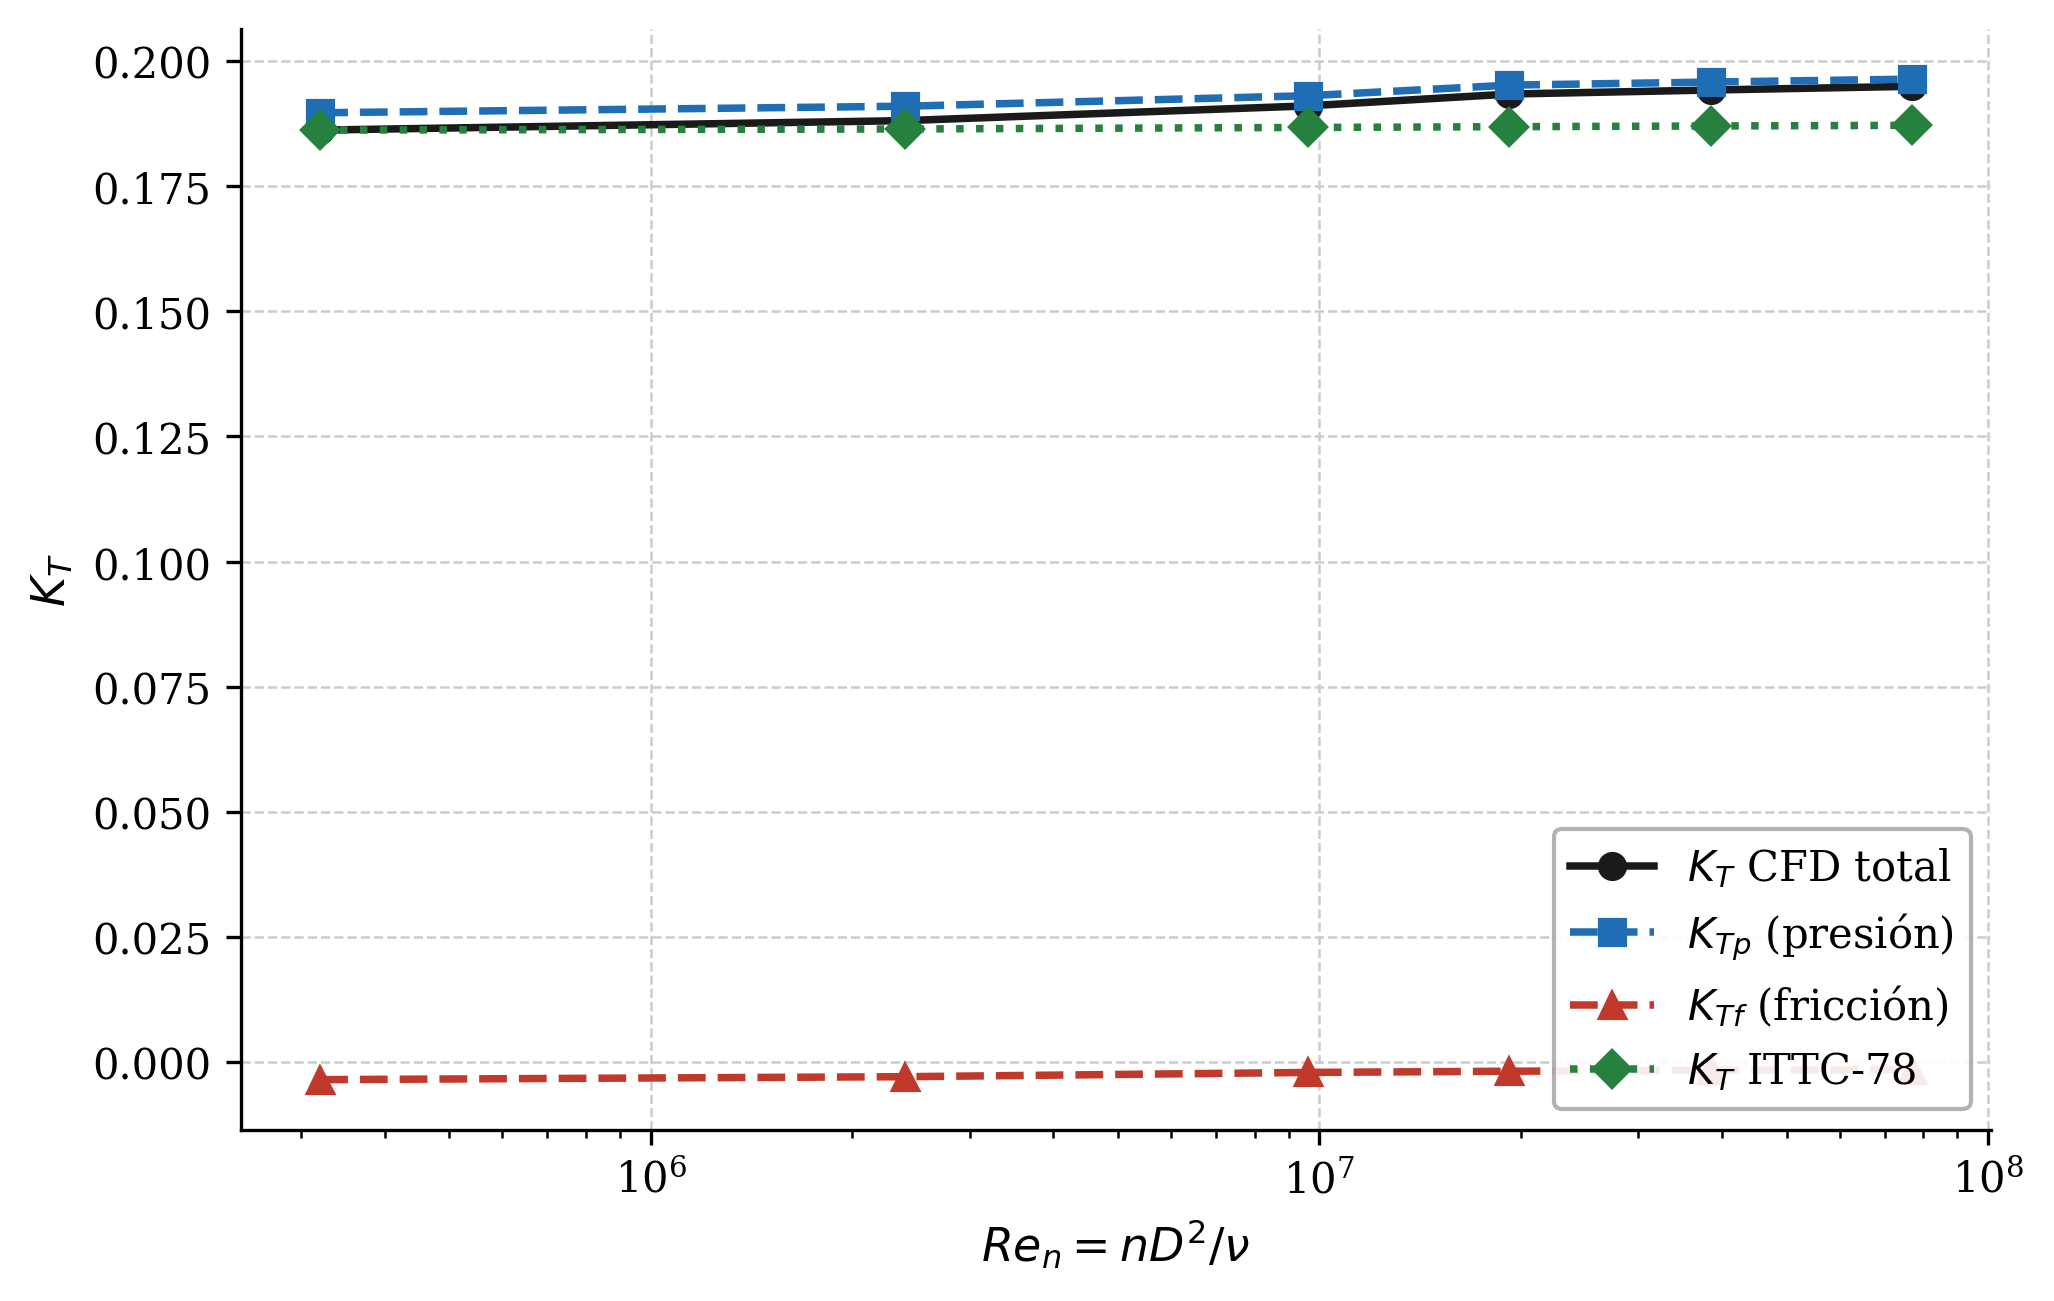
\includegraphics[width=0.75\textwidth]{images/fig1_Kt_Re.png}
\caption{Coeficientes $K_T$, $K_{Tp}$ y $K_{Tf}$ en función del número de Reynolds $Re_n = nD^2/\nu$ para el barrido de escala B4-60 a $J=0.5$. Se incluye la predicción del procedimiento ITTC-78 como referencia.}
\label{fig:kt_vs_re}
\end{figure}

\subsection{Descomposición friccional/presión ($\Delta K_{Tf}$, $\Delta K_{Tp}$, $\Delta K_{Qf}$, $\Delta K_{Qp}$)}
\label{sec:helices_descomposicion}

La descomposición de las fuerzas e integración de momentos que realiza OpenFOAM permite separar las contribuciones friccional y de presión a $K_T$ y $K_Q$ para cada escala. La Tabla~\ref{tab:delta_sweep_b460} presenta las variaciones acumuladas respecto a la referencia $D = 0.14$~m.

\begin{table}[htpb]
\centering
\caption{Variaciones de $K_T$ y $10K_Q$ respecto a $D=0.14$~m, descompuestas en contribuciones de presión y fricción. La columna $\Delta K_{Tp}/\Delta K_T$ indica la fracción del efecto de escala atribuible a la componente de presión.}
\label{tab:delta_sweep_b460}
\small
\begin{tabular}{cccccccc}
\hline
$D$ [m] & $\Delta K_T$ & $\Delta K_{Tp}$ & $\Delta K_{Tf}$ & $\frac{\Delta K_{Tp}}{\Delta K_T}$ & $10\Delta K_Q$ & $10\Delta K_{Qp}$ & $10\Delta K_{Qf}$ \\
\hline
$0.50$ & $+0.0019$ & $+0.0013$ & $+0.0006$ & $68.9\%$ & $-0.0054$ & $+0.0011$ & $-0.0065$ \\
$1.00$ & $+0.0048$ & $+0.0034$ & $+0.0014$ & $70.3\%$ & $-0.0104$ & $+0.0034$ & $-0.0137$ \\
$2.00$ & $+0.0072$ & $+0.0055$ & $+0.0017$ & $76.6\%$ & $-0.0095$ & $+0.0064$ & $-0.0159$ \\
$4.00$ & $+0.0080$ & $+0.0061$ & $+0.0019$ & $76.6\%$ & $-0.0103$ & $+0.0072$ & $-0.0176$ \\
$8.00$ & $+0.0087$ & $+0.0067$ & $+0.0020$ & $76.8\%$ & $-0.0109$ & $+0.0080$ & $-0.0190$ \\
\hline
\end{tabular}
\end{table}

El resultado más significativo de esta descomposición es que la componente de presión domina el efecto de escala en $K_T$: entre $D=1.0$ y $D=8.0$~m, la fracción $\Delta K_{Tp}/\Delta K_T$ se estabiliza en torno al $76$--$77\%$ (Figura~\ref{fig:delta_descomp}). Esto implica que aproximadamente tres cuartas partes del incremento de empuje al pasar de escala modelo a escala buque no provienen de la reducción de fricción, sino de cambios en la distribución de presiones sobre las palas asociados al adelgazamiento de la capa límite. En $K_Q$, el comportamiento es diferente: $\Delta K_{Qp}$ es positivo (el par de presión aumenta ligeramente con la escala) mientras que $\Delta K_{Qf}$ es negativo y de mayor magnitud, de modo que la reducción total de par está dominada por la componente friccional. Este comportamiento asimétrico entre empuje y par tiene implicaciones directas para la evaluación de los métodos de extrapolación, que se analizan en la sección siguiente.

\begin{figure}[htpb]
\centering
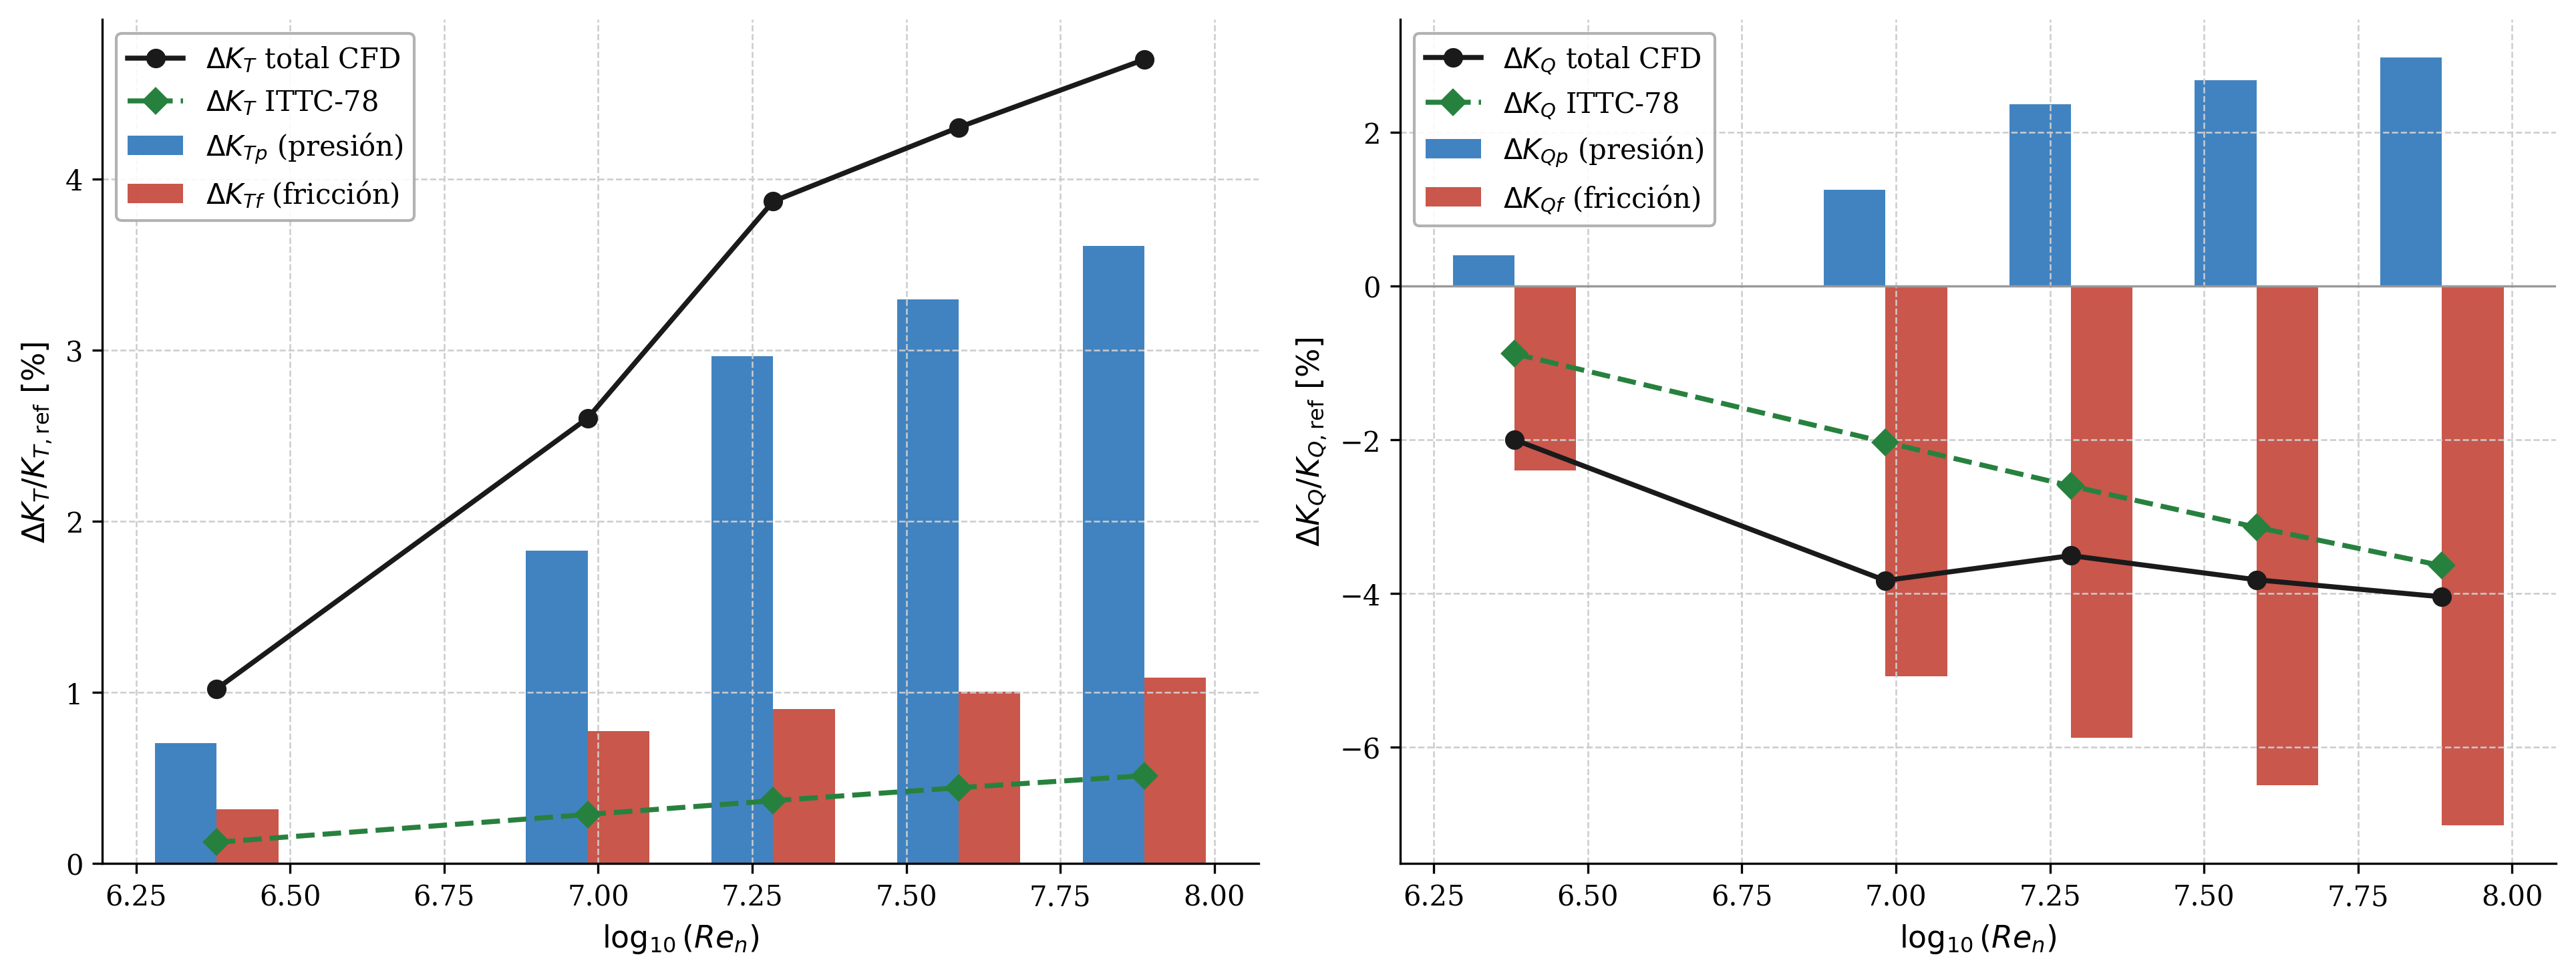
\includegraphics[width=0.95\textwidth]{images/fig2_delta_descomp.png}
\caption{Variación porcentual de $\Delta K_T$ (izquierda) y $\Delta K_Q$ (derecha) respecto al caso de referencia $D=0.14$~m, descompuesta en contribuciones de presión y fricción. Se incluye la predicción del ITTC-78.}
\label{fig:delta_descomp}
\end{figure}

% ============================================================
%  Subsección para insertar en la Sección 8.2 (Efectos de escala en la B4-60),
%  a continuación de \subsection{Descomposición friccional/presión ...}
%  (label sec:helices_descomposicion) y antes de
%  \subsection{Comparación con el procedimiento ITTC-78}.
%
%  NOTA (etiquetado de Reynolds):
%  Las figuras se rotulan con el Re_n = nD^2/nu REALIZADO de cada caso, calculado
%  con nu = 0.95653e-6 (la viscosidad real de las simulaciones). Los puntos del
%  barrido son Re_n ~ 1e4, 5e4, 1.44e5, 7.19e5, 1.44e6 y 2.5e6. Los nombres de
%  carpeta (1e5, 5e5, 1e6) NO coinciden con el Re_n realizado en tres casos, por
%  un nu inconsistente al fijar las rpm; por eso se etiqueta con el Re_n realizado.
%  Este barrido de campo (hasta Re_n ~ 2.5e6) es distinto del barrido de fuerzas
%  de la Tabla~\ref{tab:barrido_b460} (hasta Re_n ~ 7.7e7). Copiar los PNG a images/:
%    delta_cp_dorso.png, delta_cp_cara.png, radial_rms_dcp.png,
%    radial_rms_dcp_amp.png, cp_section_r07.png, cp_section_r09.png
% ============================================================
\subsection{Distribución superficial del efecto de escala en presión}
\label{sec:helices_campo_presion}
La descomposición de la Sección~\ref{sec:helices_descomposicion} establece, a partir de la integración de fuerzas, que alrededor de tres cuartas partes del incremento de empuje con la escala provienen de la componente de presión y no de la reducción de fricción. Ese resultado es, sin embargo, una magnitud integral: indica \emph{cuánto} pesa la presión, pero no \emph{dónde} sobre la pala se produce la redistribución ni cómo evoluciona con el número de Reynolds. Para esclarecer el mecanismo se analiza a continuación el campo de presión sobre la pala directamente, comparándolo entre escalas, a partir de un barrido de Reynolds dedicado de la B4-60 que abarca $Re_n$ desde $\sim\!10^{4}$ (escala modelo) hasta $\sim\!2.5\times10^{6}$. Este rango cubre el inicio y buena parte de la evolución del efecto de escala en régimen turbulento; como se muestra más abajo, la redistribución de presión se encuentra prácticamente saturada dentro de él, en consonancia con la estabilización de la fracción $\Delta K_{Tp}/\Delta K_T$ observada en la Tabla~\ref{tab:delta_sweep_b460}.
El coeficiente de presión sobre la pala se define, siguiendo la convención habitual para propulsores, respecto de la presión dinámica construida con la velocidad resultante en la sección de referencia a $r/R=0.7$,
\begin{equation}
C_p = \frac{p - p_\infty}{\tfrac{1}{2}\rho\,V_{0.7R}^2},
\qquad
V_{0.7R}^2 = V_a^2 + \left(0.7\,\pi n D\right)^2,
\qquad
V_a = J\,n\,D,
\label{eq:cp_helice}
\end{equation}
de modo que $C_p$ resulta adimensional y comparable entre escalas. El efecto de escala local se caracteriza mediante el campo de diferencia
\begin{equation}
\Delta C_p = C_{p}(Re_n) - C_{p}(Re_{n,\mathrm{ref}}),
\label{eq:dcp_helice}
\end{equation}
evaluado sobre la geometría de la escala de referencia (escala modelo). Como todas las mallas se obtienen escalando uniformemente una única malla base, al adimensionalizar las coordenadas por el diámetro las superficies de dos escalas cualesquiera se superponen de forma exacta, y la diferencia de la Ecuación~\ref{eq:dcp_helice} se calcula punto a punto sin interpolación ni ambigüedad. Cabe destacar que las tres métricas de campo empleadas en esta subsección --el mapa de $\Delta C_p$, su perfil radial y su amplitud-- son puramente descriptivas: cuantifican la magnitud y la localización de la redistribución de presión, y no reconstruyen fuerzas. La contribución neta de la presión al empuje y al par sigue siendo la reportada por la integración de OpenFOAM en la Sección~\ref{sec:helices_descomposicion}.
\paragraph{Distribución sobre la pala.} La Figura~\ref{fig:dcp_map} muestra el campo $\Delta C_p$ entre la escala modelo y la mayor escala del barrido ($Re_n\approx 2.5\times10^{6}$), sobre el dorso (lado de succión) y la cara (lado de presión). El contraste entre ambos lados es marcado. La cara permanece casi invariable con la escala, salvo una franja delgada en las proximidades del borde de ataque hacia la punta. El dorso, en cambio, concentra prácticamente toda la redistribución: la succión se profundiza ($\Delta C_p<0$) a lo largo del borde de ataque --de forma más intensa hacia la punta-- mientras que hacia el borde de salida y la zona media-externa la presión se recupera ($\Delta C_p>0$). Este patrón es la firma esperada del adelgazamiento de la capa límite al aumentar $Re_n$: un pico de succión de borde de ataque más marcado y una mejor recuperación de presión aguas abajo. El resultado localiza espacialmente la componente de presión que la descomposición de fuerzas cuantifica de forma global y confirma que actúa esencialmente sobre el lado de succión. Los valores extremos de $\Delta C_p$ se ubican en la esquina punta--borde de ataque; conviene recordar que esa zona, junto con el borde de salida, es la de mayor sensibilidad a la discretización geométrica del extremo de pala, por lo que su magnitud puntual no debe sobreinterpretarse, si bien la redistribución en el cuerpo de la pala es robusta.
\begin{figure}[htpb]
\centering
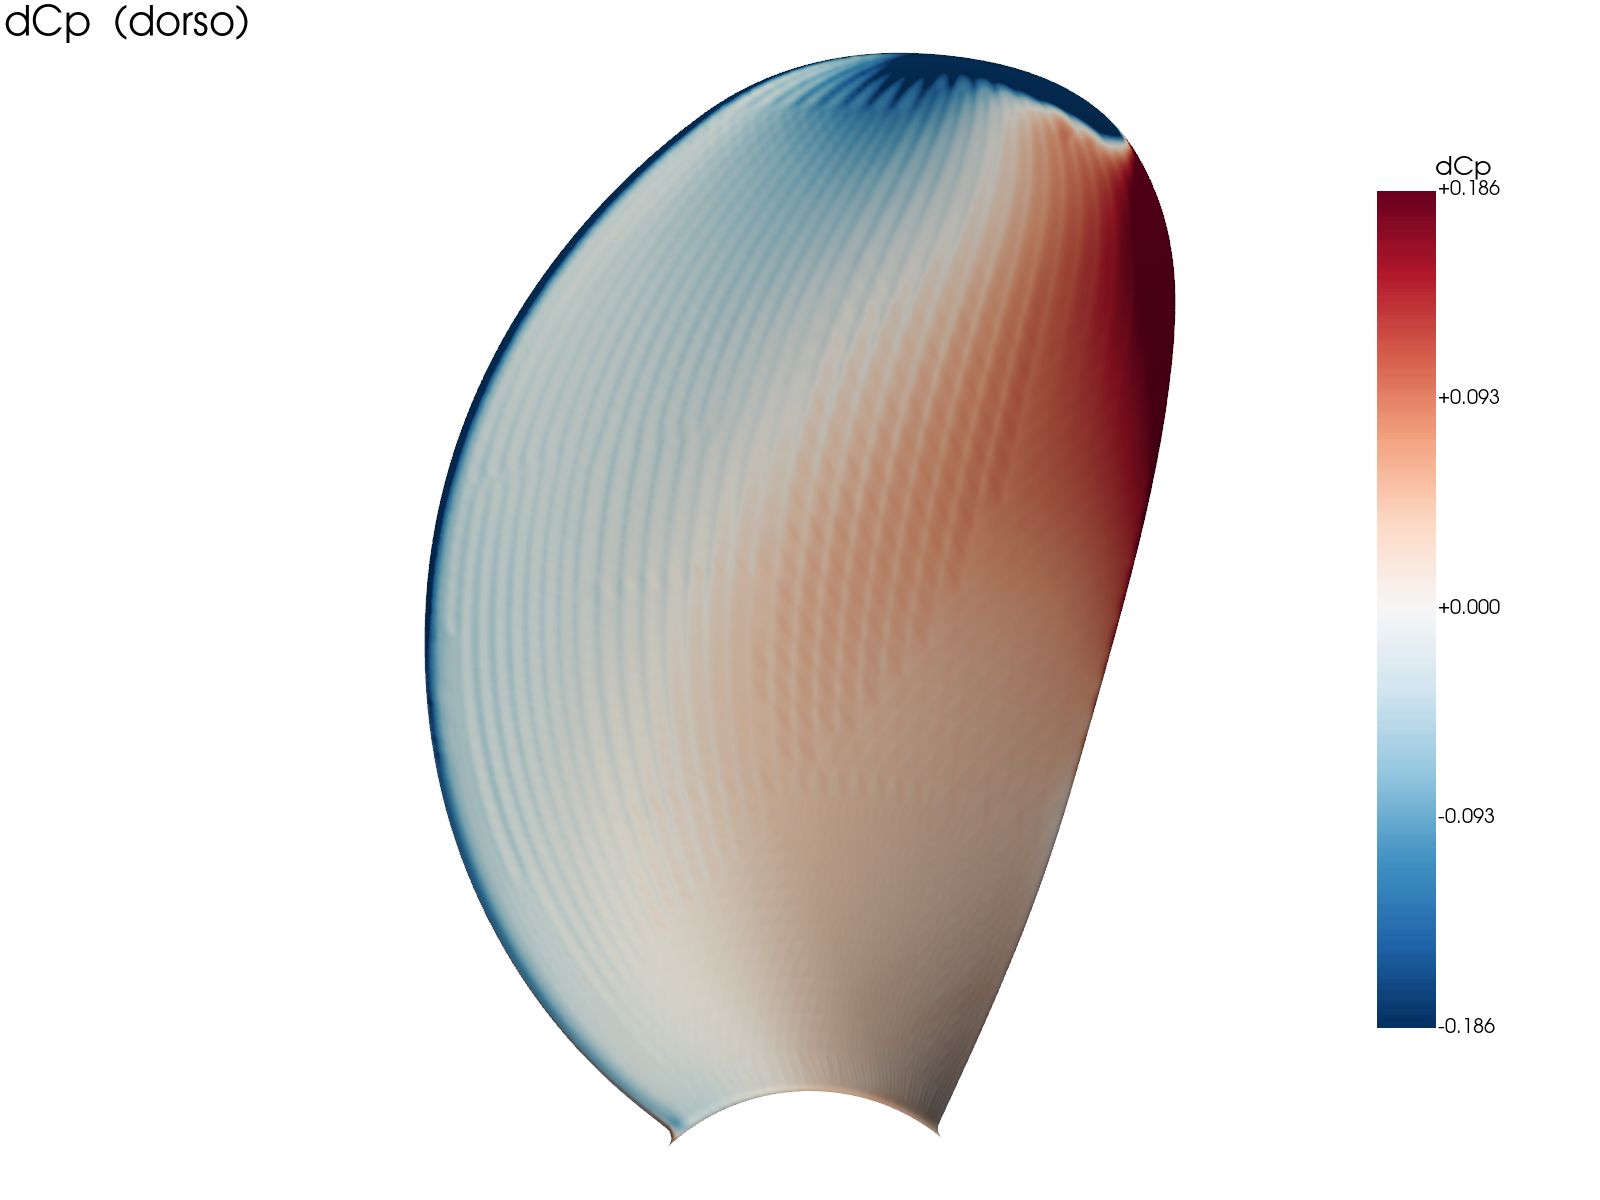
\includegraphics[width=0.48\textwidth]{images/delta_cp_dorso.png}\hfill
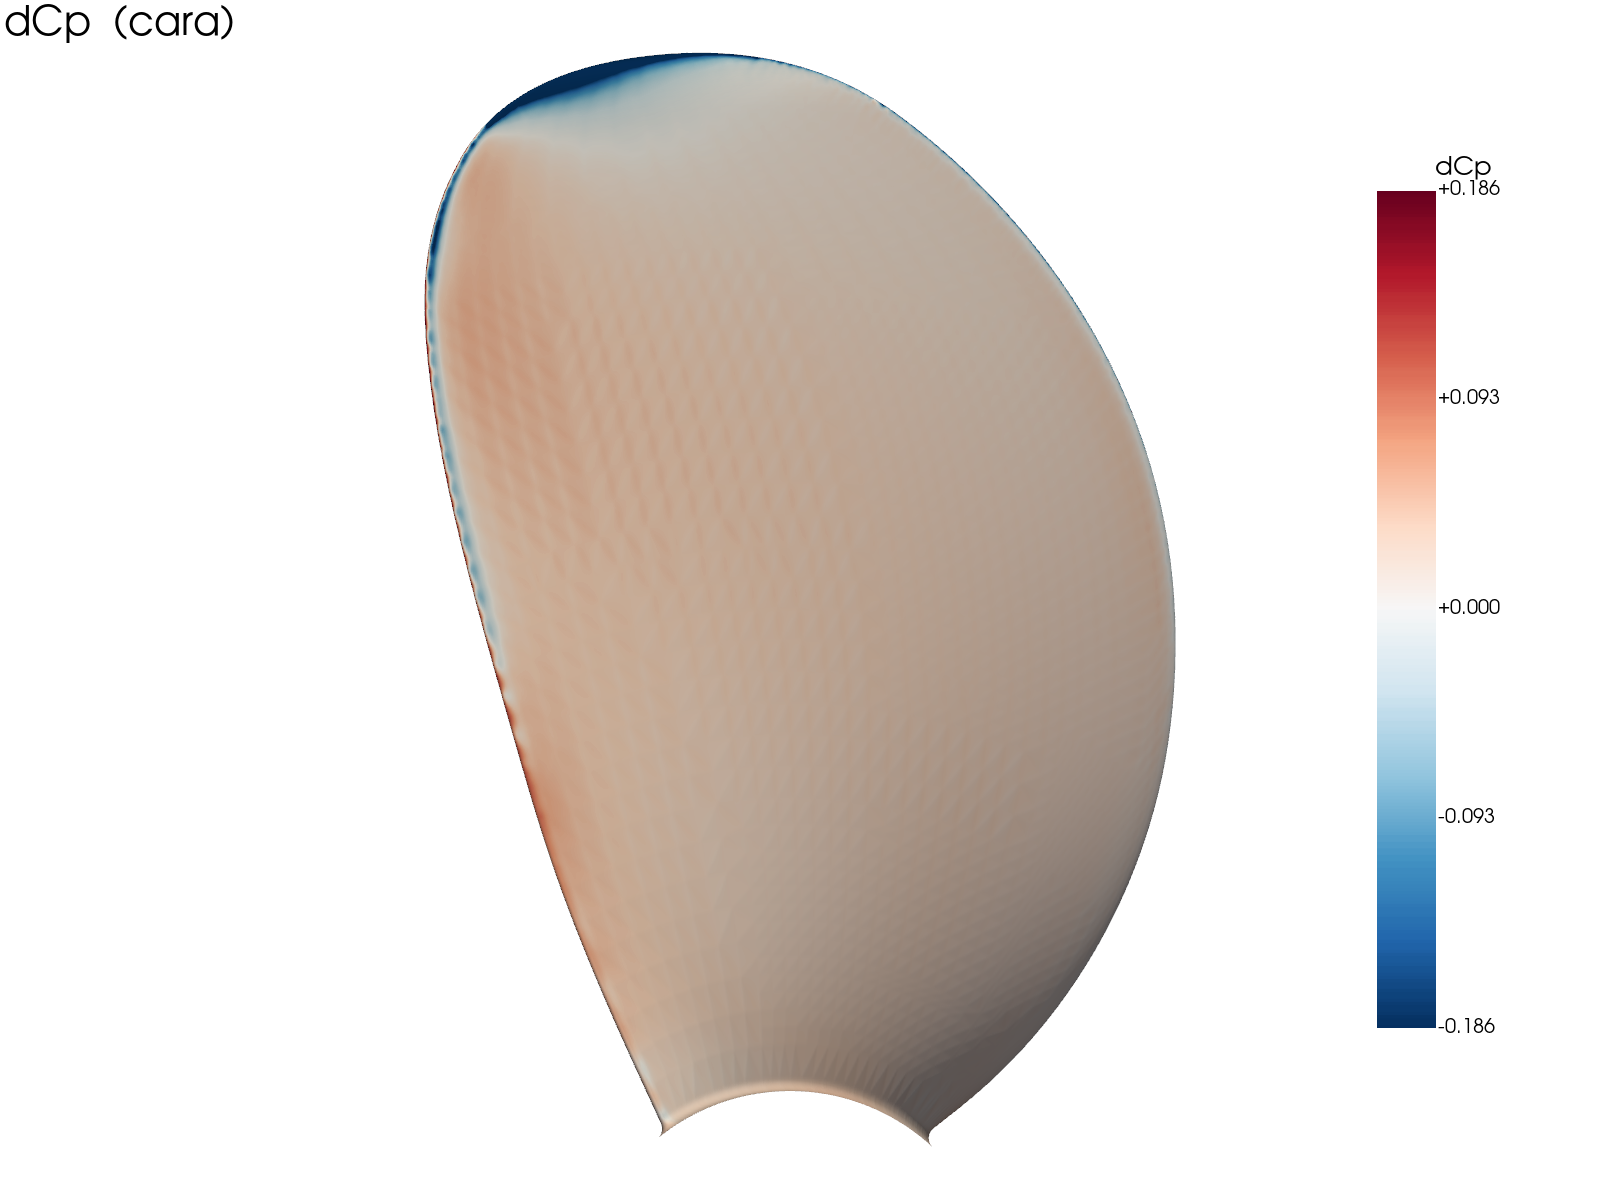
\includegraphics[width=0.48\textwidth]{images/delta_cp_cara.png}
\caption{Campo de diferencia $\Delta C_p = C_p(Re_n) - C_p(Re_{n,\mathrm{ref}})$ entre la escala modelo y $Re_n\approx 2.5\times10^{6}$, sobre el dorso (izquierda, lado de succión) y la cara (derecha, lado de presión) de la pala B4-60. El rango de color es simétrico y se recorta al percentil 98 de $|\Delta C_p|$ para evitar que los extremos de punta y bordes dominen la escala.}
\label{fig:dcp_map}
\end{figure}
\paragraph{Distribución radial.} Para cuantificar la observación anterior, el mapa se colapsa a una curva radial mediante el valor cuadrático medio de $\Delta C_p$ pesado por el área de celda en bandas de radio constante,
\begin{equation}
\mathrm{RMS}_{\Delta C_p}(r/R) = \sqrt{\frac{\sum_i \Delta C_{p,i}^{\,2}\,|A_i|}{\sum_i |A_i|}},
\label{eq:rms_dcp}
\end{equation}
donde la suma recorre las celdas de cada banda. La Figura~\ref{fig:dcp_radial} presenta esta curva para todas las escalas del barrido. En todo el tramo interior y medio de la pala la amplitud del efecto crece de forma suave y monótona hacia la punta, con las escalas perfectamente ordenadas por $Re_n$: la redistribución de presión es despreciable en la raíz y se intensifica hacia la mitad externa, coherentemente con lo observado en el mapa. Se excluye del gráfico la región $r/R>0.95$, donde el vórtice de punta y la discretización del borde dominan la señal y no son representativos de la redistribución asociada a la capa límite.
\begin{figure}[htpb]
\centering
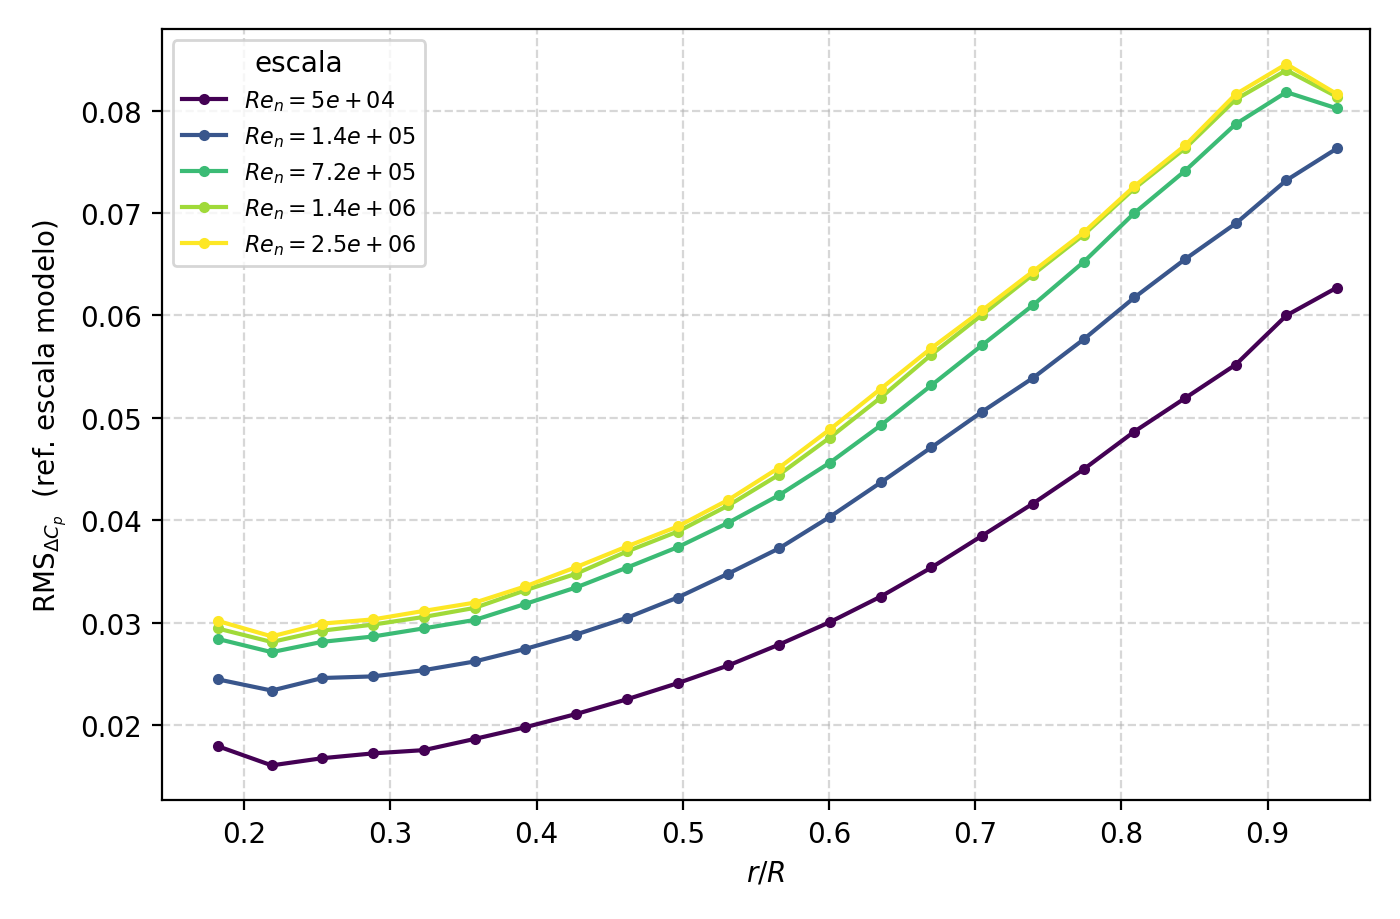
\includegraphics[width=0.75\textwidth]{images/radial_rms_dcp.png}
\caption{Valor cuadrático medio radial de $\Delta C_p$ (Ecuación~\ref{eq:rms_dcp}), referido a la escala modelo, en función de $r/R$ para las escalas del barrido. Se excluye $r/R>0.95$ (vórtice de punta y borde, sensibles a la discretización).}
\label{fig:dcp_radial}
\end{figure}
\paragraph{Convergencia con el número de Reynolds.} La Figura~\ref{fig:dcp_amp} colapsa cada campo a una única amplitud --el RMS de $\Delta C_p$ pesado por área sobre la pala hasta $r/R<0.95$-- y la representa en función de $Re_n$. La curva, anclada en cero en la escala modelo por definición, crece empinadamente en el primer tramo y se aplana hacia los Reynolds altos: más de la mitad de la redistribución de presión ya está presente en $Re_n\sim 5\times10^{4}$ y del orden del $95\%$ hacia $Re_n\sim 7\times10^{5}$, con los dos puntos de mayor Reynolds prácticamente indistinguibles. Este comportamiento de saturación es consistente con la estabilización de la fracción $\Delta K_{Tp}/\Delta K_T$ en torno al $76$--$77\%$ observada en la descomposición de fuerzas (Tabla~\ref{tab:delta_sweep_b460}) a partir de $D\gtrsim 1$~m, e implica que la mayor parte del efecto de escala en presión se alcanza a Reynolds moderados. Debe subrayarse que esta amplitud es una medida sin signo de la \emph{magnitud} de la redistribución del campo, no de su aporte neto al empuje; este último es el $\Delta K_{Tp}$ de la Sección~\ref{sec:helices_descomposicion}.
\begin{figure}[htpb]
\centering
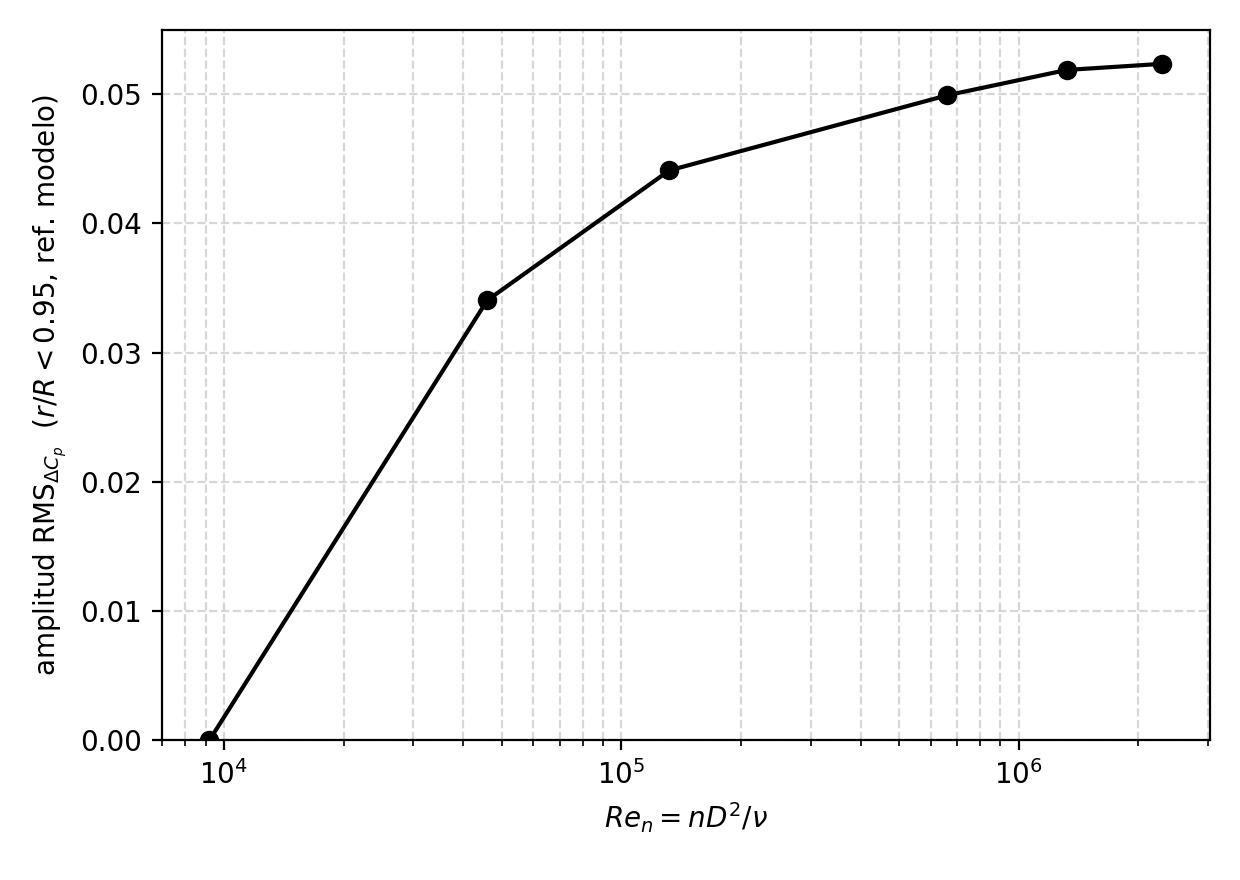
\includegraphics[width=0.7\textwidth]{images/radial_rms_dcp_amp.png}
\caption{Amplitud global de la redistribución de presión (RMS de $\Delta C_p$ pesado por área, $r/R<0.95$, referido a la escala modelo) en función de $Re_n = nD^2/\nu$. La curva evidencia la saturación del efecto de escala en presión hacia $Re_n\sim10^{6}$.}
\label{fig:dcp_amp}
\end{figure}
\paragraph{Mecanismo seccional.} Finalmente, la Figura~\ref{fig:cp_secciones} presenta la distribución de $C_p$ en función de la coordenada de cuerda $x/c$ en dos secciones representativas, $r/R=0.7$ y $r/R=0.9$, para todas las escalas. Cada sección se obtiene como la isolínea de radio constante sobre la pala, un corte puramente geométrico. En el dorso, el pico de succión de borde de ataque se profundiza sistemáticamente al aumentar $Re_n$ --desde la escala modelo, de pico más chato, hasta las escalas mayores-- y hacia el borde de salida las curvas de mayor Reynolds caen por debajo de la de escala modelo, reflejando la mejor recuperación de presión de la capa límite adelgazada. El efecto es más pronunciado en $r/R=0.9$ que en $r/R=0.7$, en concordancia con la concentración hacia la punta ya evidenciada en las Figuras~\ref{fig:dcp_map} y \ref{fig:dcp_radial}. En la cara, por el contrario, las curvas de las distintas escalas se superponen casi por completo, confirmando que la redistribución de presión reside casi enteramente en el lado de succión. Este diagnóstico seccional es el análogo, como estudio de convergencia con la escala, del que se aplica a la hélice de la Sección~\ref{sec:helice_coreana} para el mecanismo transicional.
\begin{figure}[htpb]
\centering
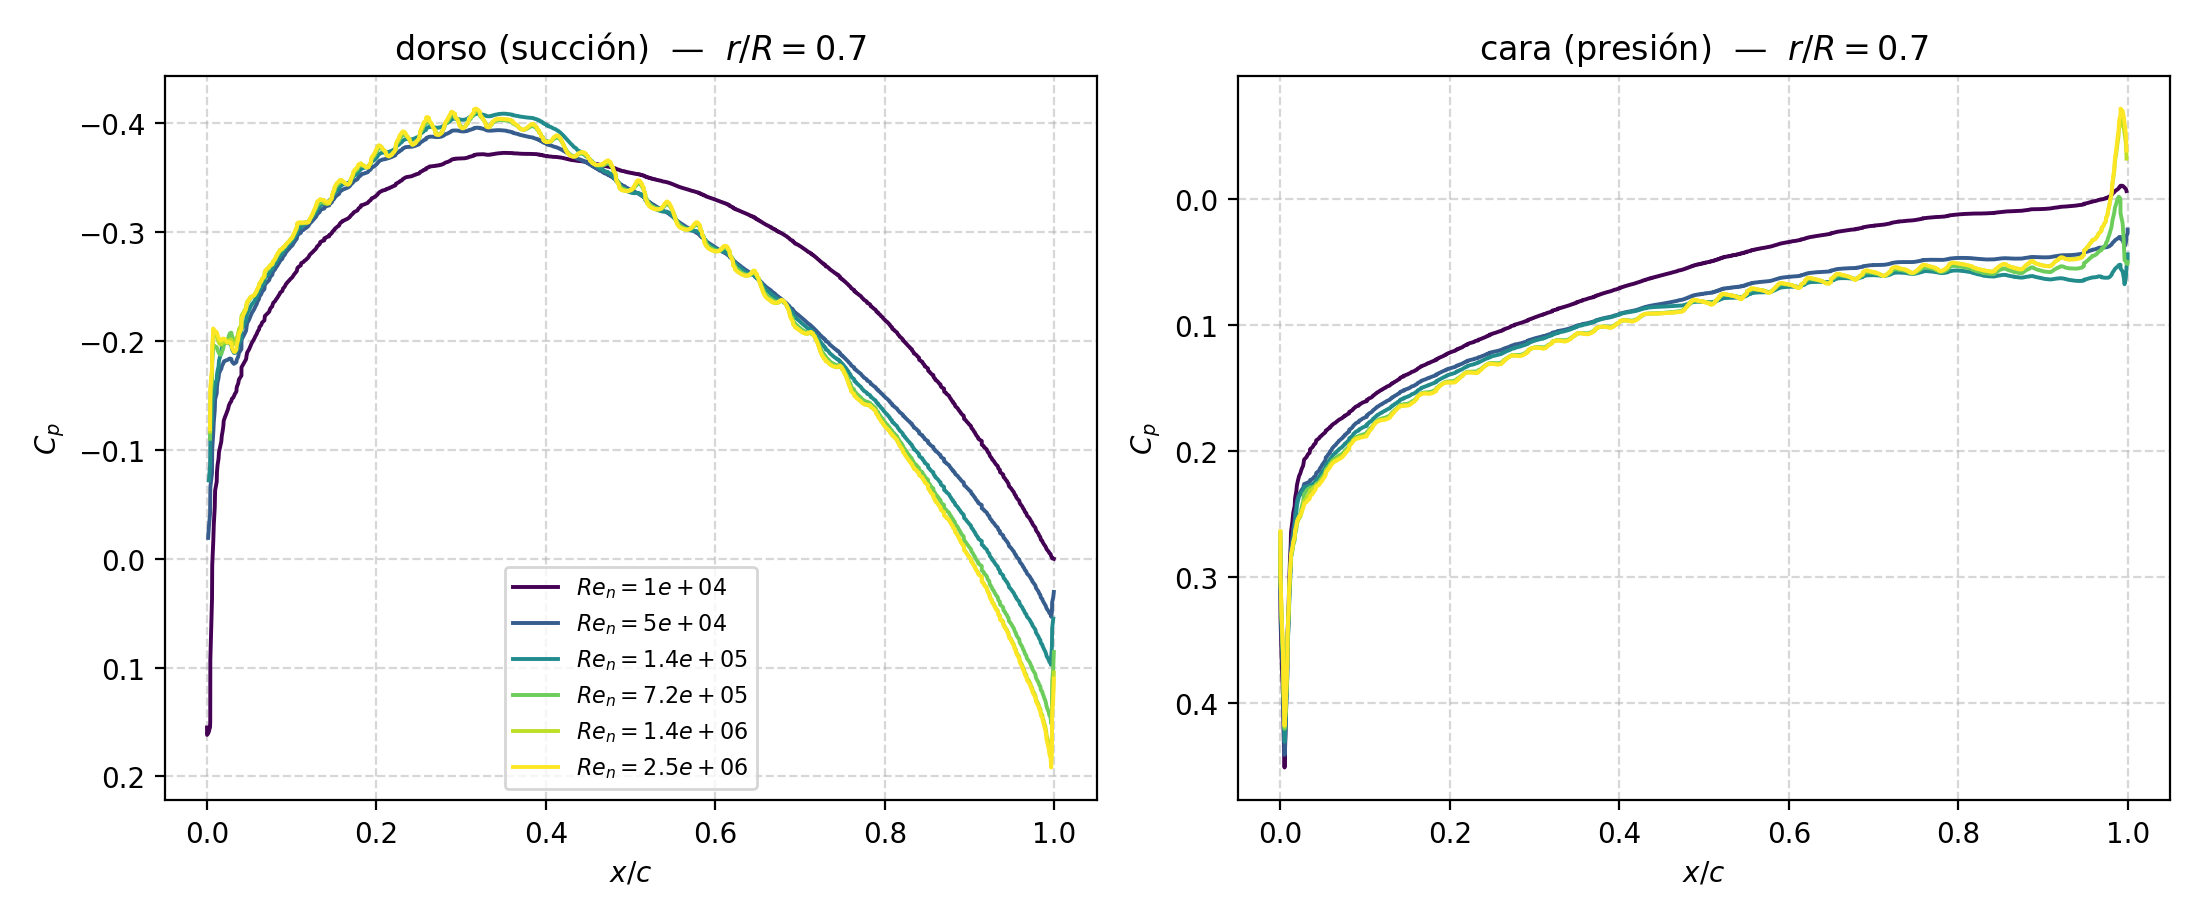
\includegraphics[width=0.92\textwidth]{images/cp_section_r07.png}\\[2pt]
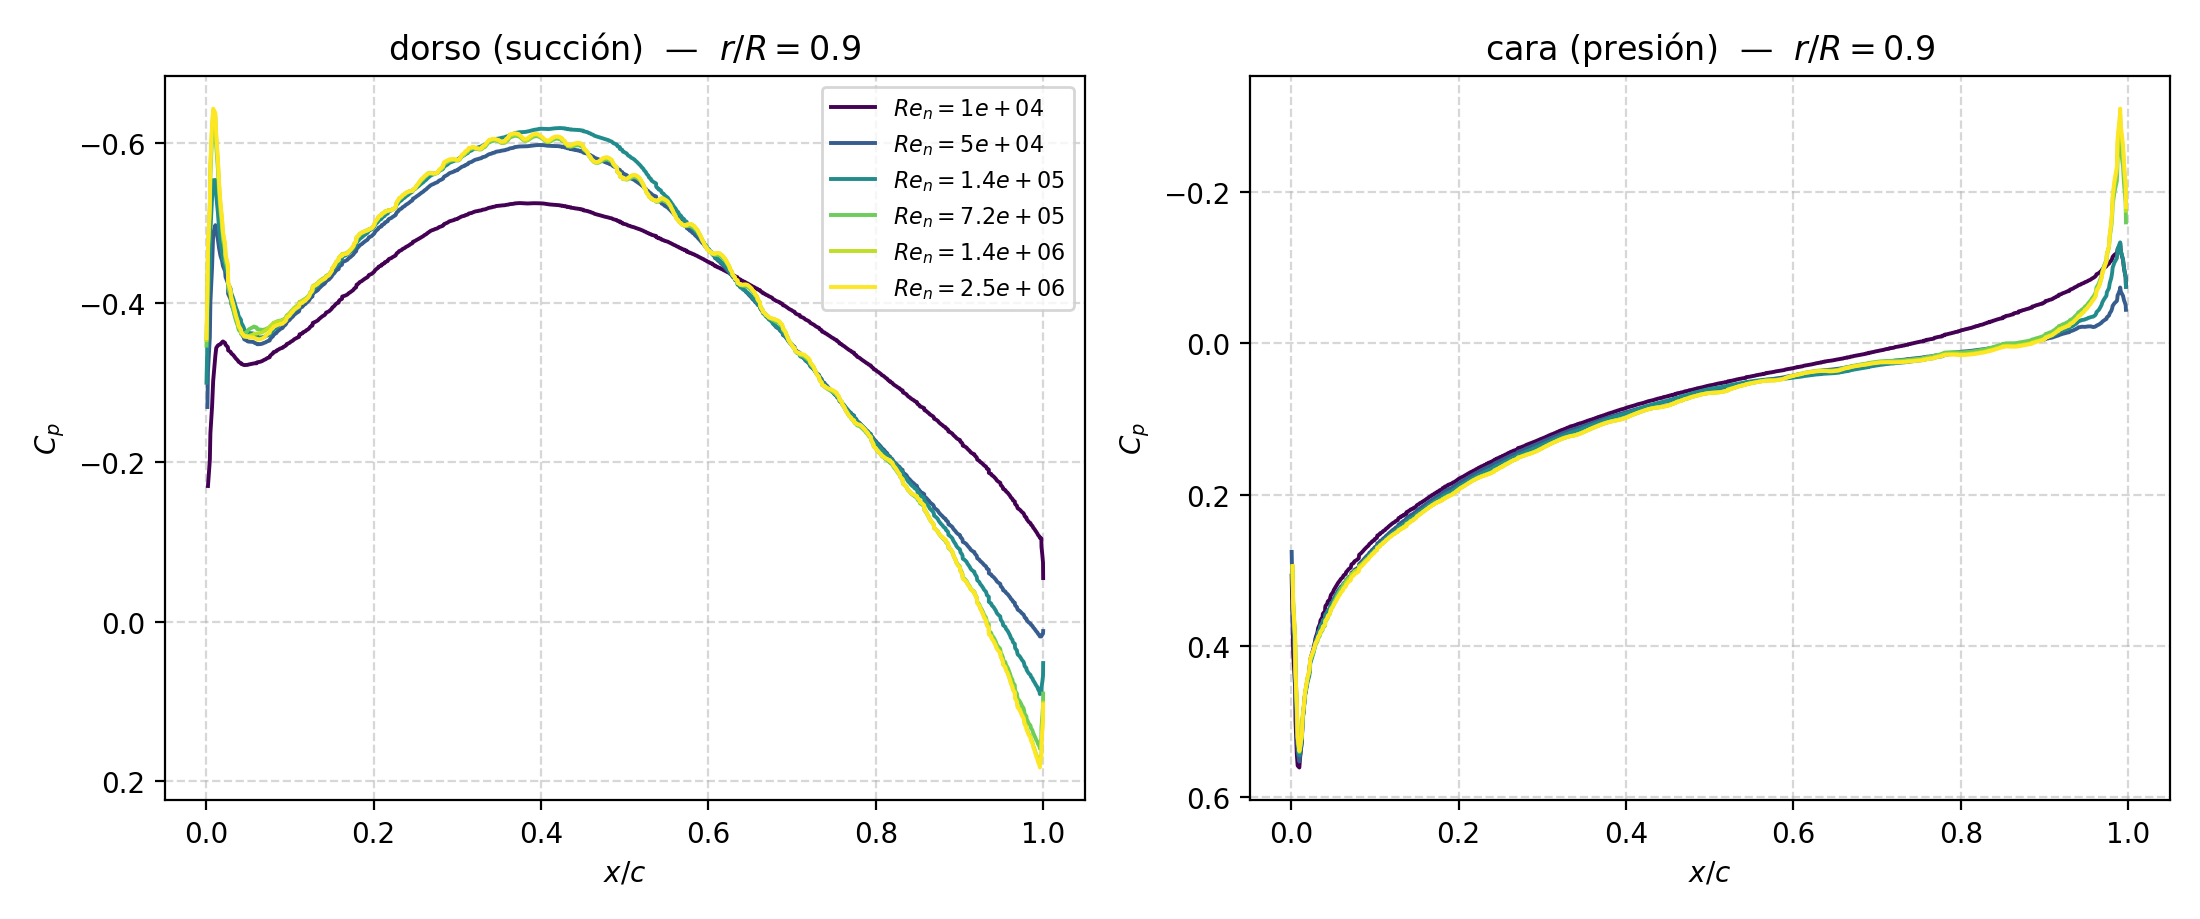
\includegraphics[width=0.92\textwidth]{images/cp_section_r09.png}
\caption{Distribución de $C_p$ a lo largo de la cuerda ($x/c$) en las secciones $r/R=0.7$ (arriba) y $r/R=0.9$ (abajo), para las escalas del barrido, separada en dorso (succión, izquierda) y cara (presión, derecha). El eje de $C_p$ está invertido (succión hacia arriba). Se aprecia el pico de succión de borde de ataque profundizándose con $Re_n$ sobre el dorso y la escasa sensibilidad de la cara.}
\label{fig:cp_secciones}
\end{figure}
En conjunto, las Figuras~\ref{fig:dcp_map}--\ref{fig:cp_secciones} corroboran, a nivel del campo de presión, el resultado obtenido por integración de fuerzas: el efecto de escala en régimen turbulento sobre la B4-60 posee una componente de presión dominante y espacialmente coherente, que el procedimiento ITTC-78 --al suponer $\Delta K_{Tp}=0$-- ignora por completo. Más aún, permiten precisar su naturaleza: se trata de una redistribución concentrada en el lado de succión de la mitad externa de la pala, que se intensifica hacia la punta y que satura a Reynolds moderados. Esta caracterización espacial refuerza la conclusión, desarrollada en la sección siguiente, de que la corrección puramente friccional del ITTC-78 es estructuralmente incapaz de capturar el efecto de escala de esta hélice.

\subsection{Comparación con el procedimiento ITTC-78}
\label{sec:helices_ittc78}

El procedimiento ITTC-78 corrige los coeficientes hidrodinámicos de modelo a escala buque mediante la diferencia de coeficiente de fricción de placa plana $\Delta C_D$ evaluada a $r/R = 0.75$, según las expresiones presentadas en la Sección~\ref{sec:ittc78_helices_metodo}. Esta corrección asume implícitamente que el efecto de escala es de naturaleza puramente friccional, es decir, que $\Delta K_{Tp} = 0$. Los resultados del CFD demuestran que esta hipótesis es incorrecta para la B4-60.

La Tabla~\ref{tab:ittc_vs_cfd} compara las predicciones del ITTC-78 y del CFD para $D = 8.0$~m, tomando $D = 0.14$~m como referencia de modelo.

\begin{table}[htpb]
\centering
\caption{Comparación entre ITTC-78 y CFD a $D = 8.0$~m ($J = 0.5$), tomando $D = 0.14$~m como referencia.}
\label{tab:ittc_vs_cfd}
\begin{tabular}{lccc}
\hline
 & ITTC-78 & CFD SST & Diferencia \\
\hline
$K_T$   & $0.1862$ & $0.1949$ & $+0.0087$ $(+4.7\%)$ \\
$10K_Q$ & $0.2618$ & $0.2593$ & $-0.0025$ $(-1.0\%)$ \\
$\eta_0$ & $0.5540$ & $0.5982$ & $+0.0442$ $(+8.0\%)$ \\
\hline
\end{tabular}
\end{table}

El ITTC-78 subestima $K_T$ en $+4.7\%$ respecto al CFD a escala buque, precisamente porque no contempla el incremento de la componente de presión. Para $10K_Q$ la diferencia es menor ($-1.0\%$), dado que las contribuciones friccional y de presión evolucionan en sentidos opuestos y se compensan parcialmente. El efecto acumulado sobre la eficiencia es significativo: el ITTC-78 predice $\eta_0 = 0.554$ frente a $\eta_0 = 0.598$ del CFD, una diferencia de $+8.0\%$ que representaría una subestimación relevante en el diseño de la instalación propulsora. Las Figuras~\ref{fig:gap_fraccion} y~\ref{fig:delta_vs_D} sintetizan gráficamente esta comparación: la primera muestra la brecha $K_{T,\mathrm{CFD}}-K_{T,\mathrm{ITTC}}$ en función del diámetro y la fracción del efecto de escala atribuible a la presión frente a otras geometrías, y la segunda, la variación de $\Delta K_T$ y $10\,\Delta K_Q$ con el diámetro descompuesta en presión y fricción, junto con la predicción del ITTC-78.

\begin{figure}[htpb]
\centering
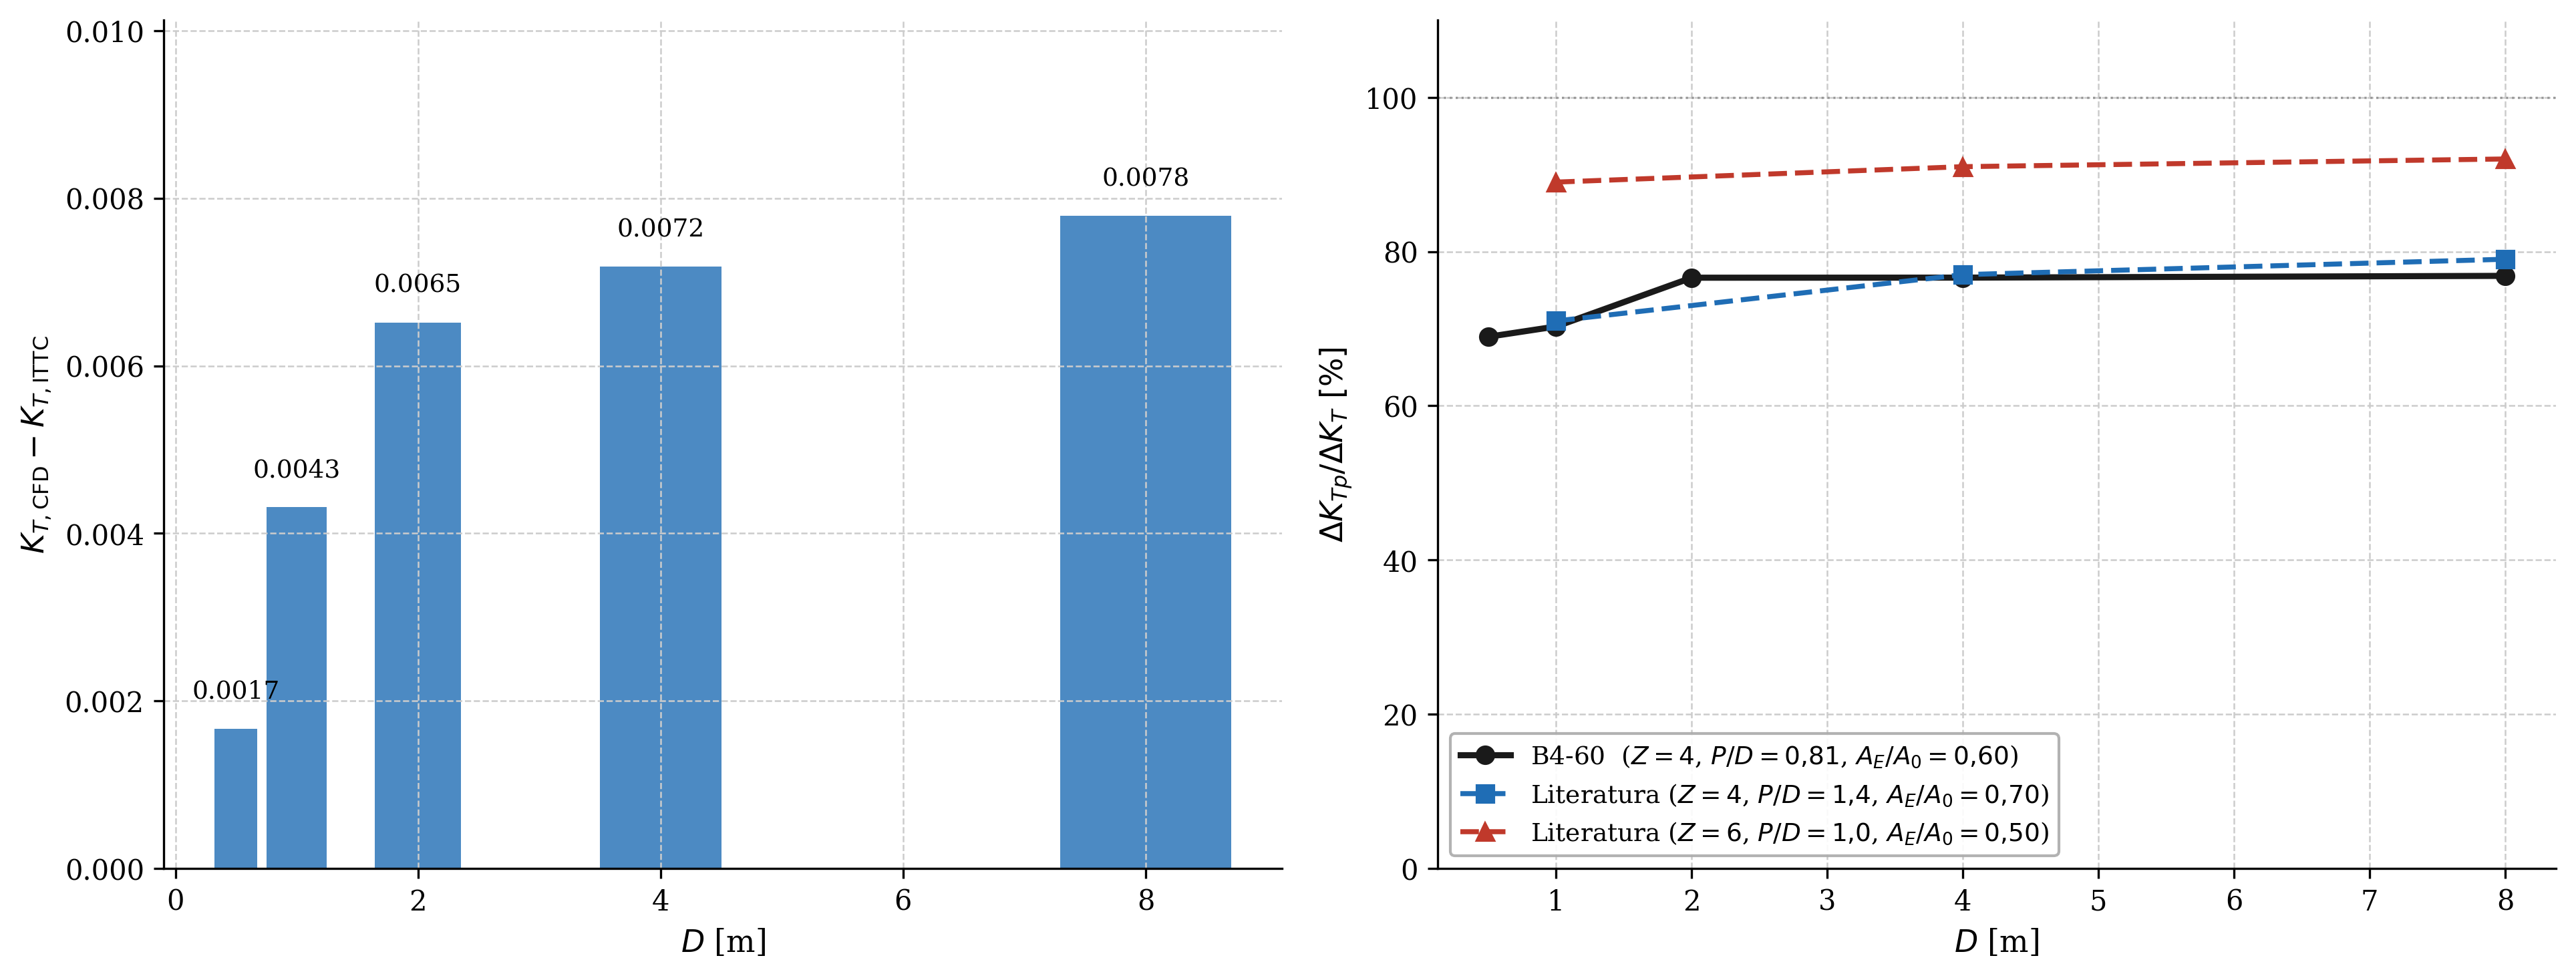
\includegraphics[width=0.95\textwidth]{images/fig4_gap_fraccion.png}
\caption{Izquierda: diferencia $K_{T,\mathrm{CFD}} - K_{T,\mathrm{ITTC}}$ en función del diámetro. Derecha: fracción del efecto de escala en $K_T$ atribuible a la componente de presión ($\Delta K_{Tp}/\Delta K_T$), comparada con datos de la literatura para otras geometrías.}
\label{fig:gap_fraccion}
\end{figure}

\begin{figure}[htpb]
\centering
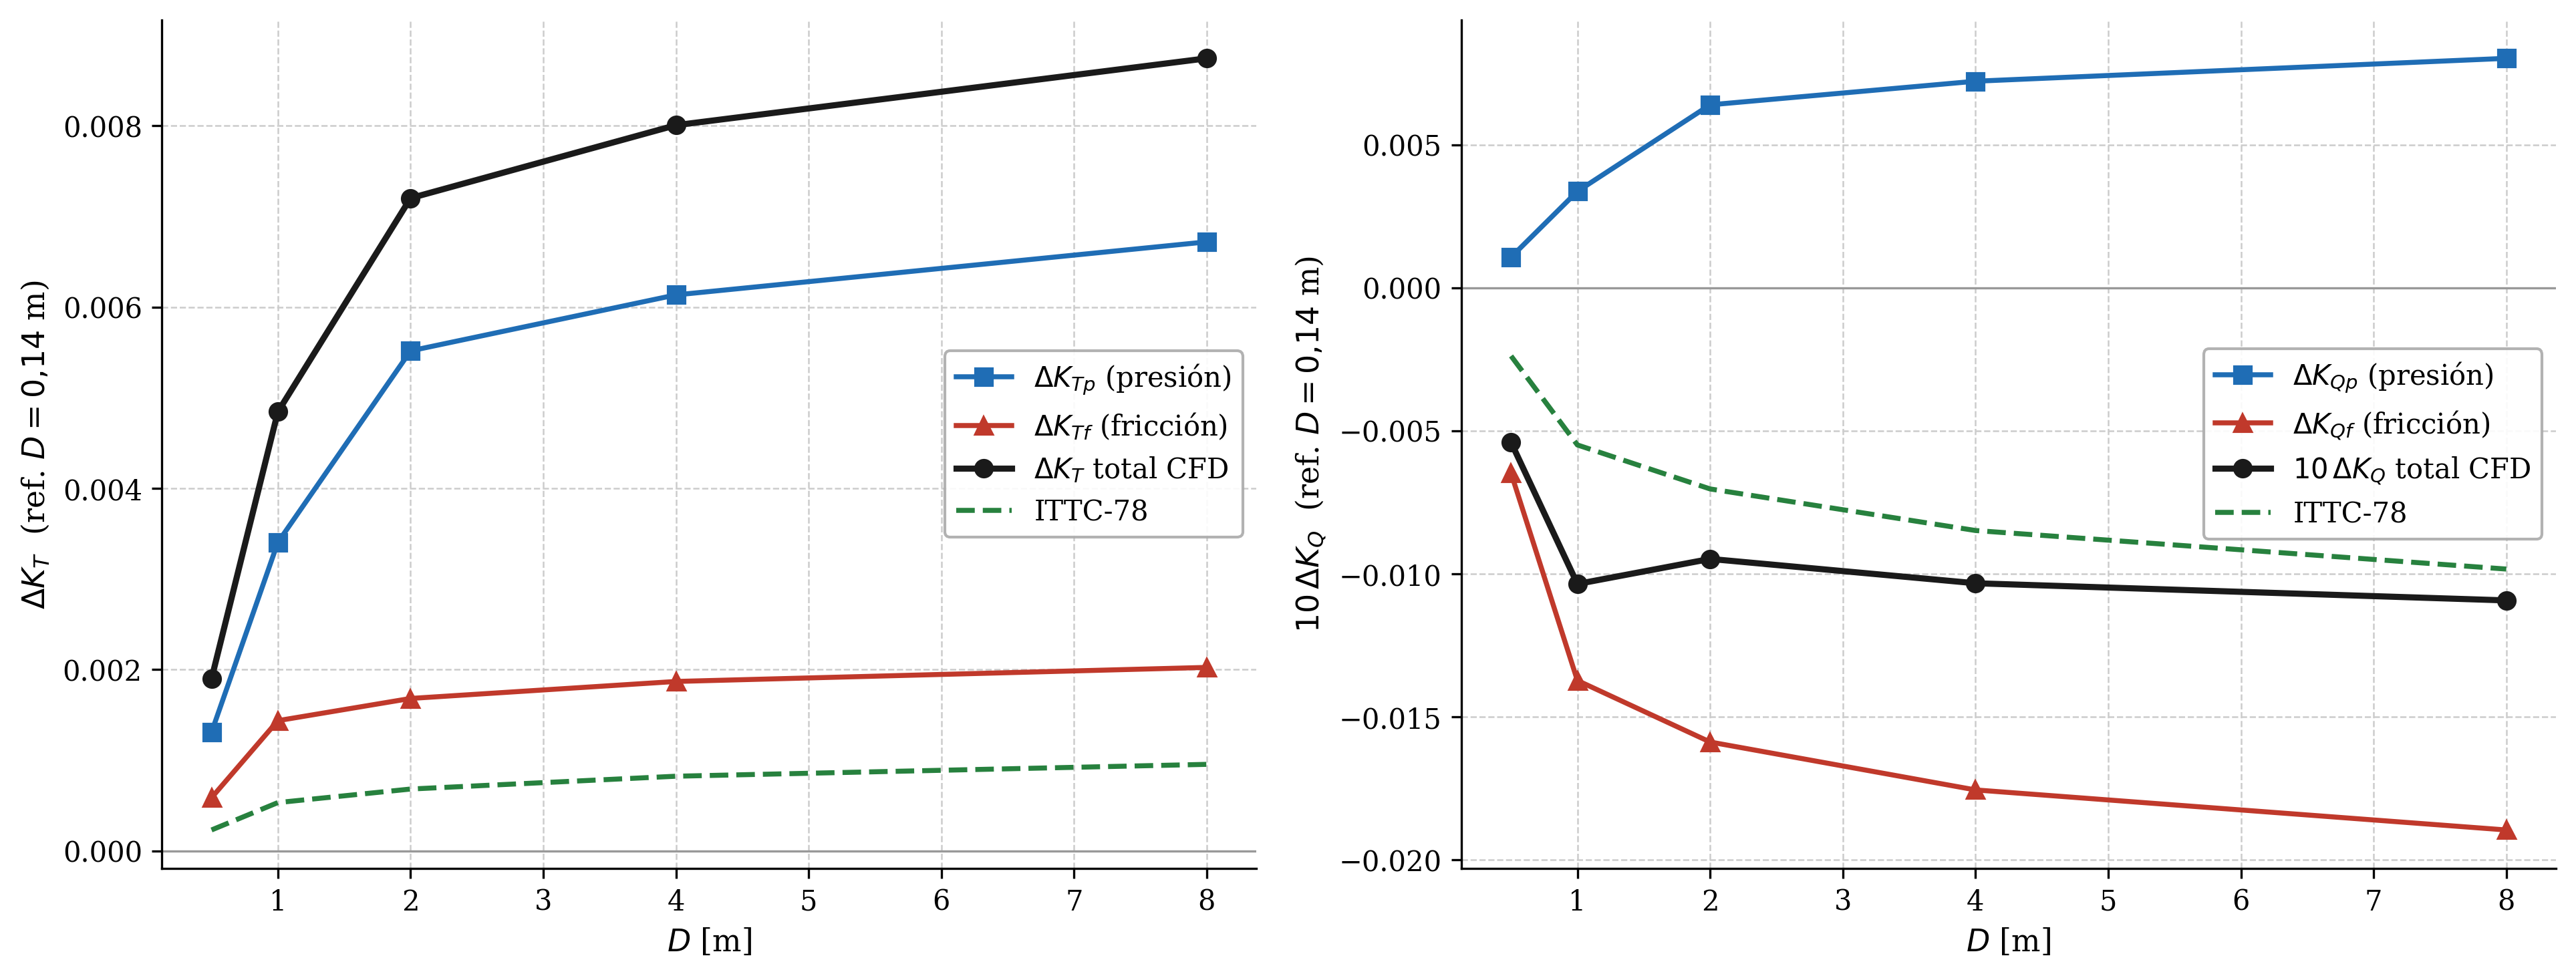
\includegraphics[width=0.95\textwidth]{images/fig3_delta_vs_D.png}
\caption{Variación de $\Delta K_T$ (izquierda) y $10\,\Delta K_Q$ (derecha) en función del diámetro, con descomposición en componentes de presión y fricción. Se incluye la predicción del ITTC-78.}
\label{fig:delta_vs_D}
\end{figure}

\subsection{Eficiencia en escala buque: comparación de métodos}
\label{sec:helices_eficiencia}

La Figura~\ref{fig:eficiencia_metodos} compara la evolución de $\eta_0$ con $Re_n$ para tres alternativas de extrapolación: el procedimiento ITTC-78 (M1), el CFD SST directo (M2) y la aplicación sin corrección del diagrama de modelo (M3). En $Re_n \approx 3.2 \times 10^5$ (D=0.14~m, escala modelo) los tres métodos coinciden por definición. A medida que $Re_n$ crece, M2 y M1 divergen progresivamente: a $D=8.0$~m ($Re_n \approx 7.7 \times 10^7$) el CFD predice un incremento de eficiencia de $+9.1\%$ respecto al modelo, mientras que el ITTC-78 solo estima $+1.1\%$. La diferencia entre ambos métodos, de $8.0$ puntos porcentuales a la mayor escala analizada, refleja la contribución ignorada de la componente de presión al efecto de escala.

\begin{figure}[htpb]
\centering
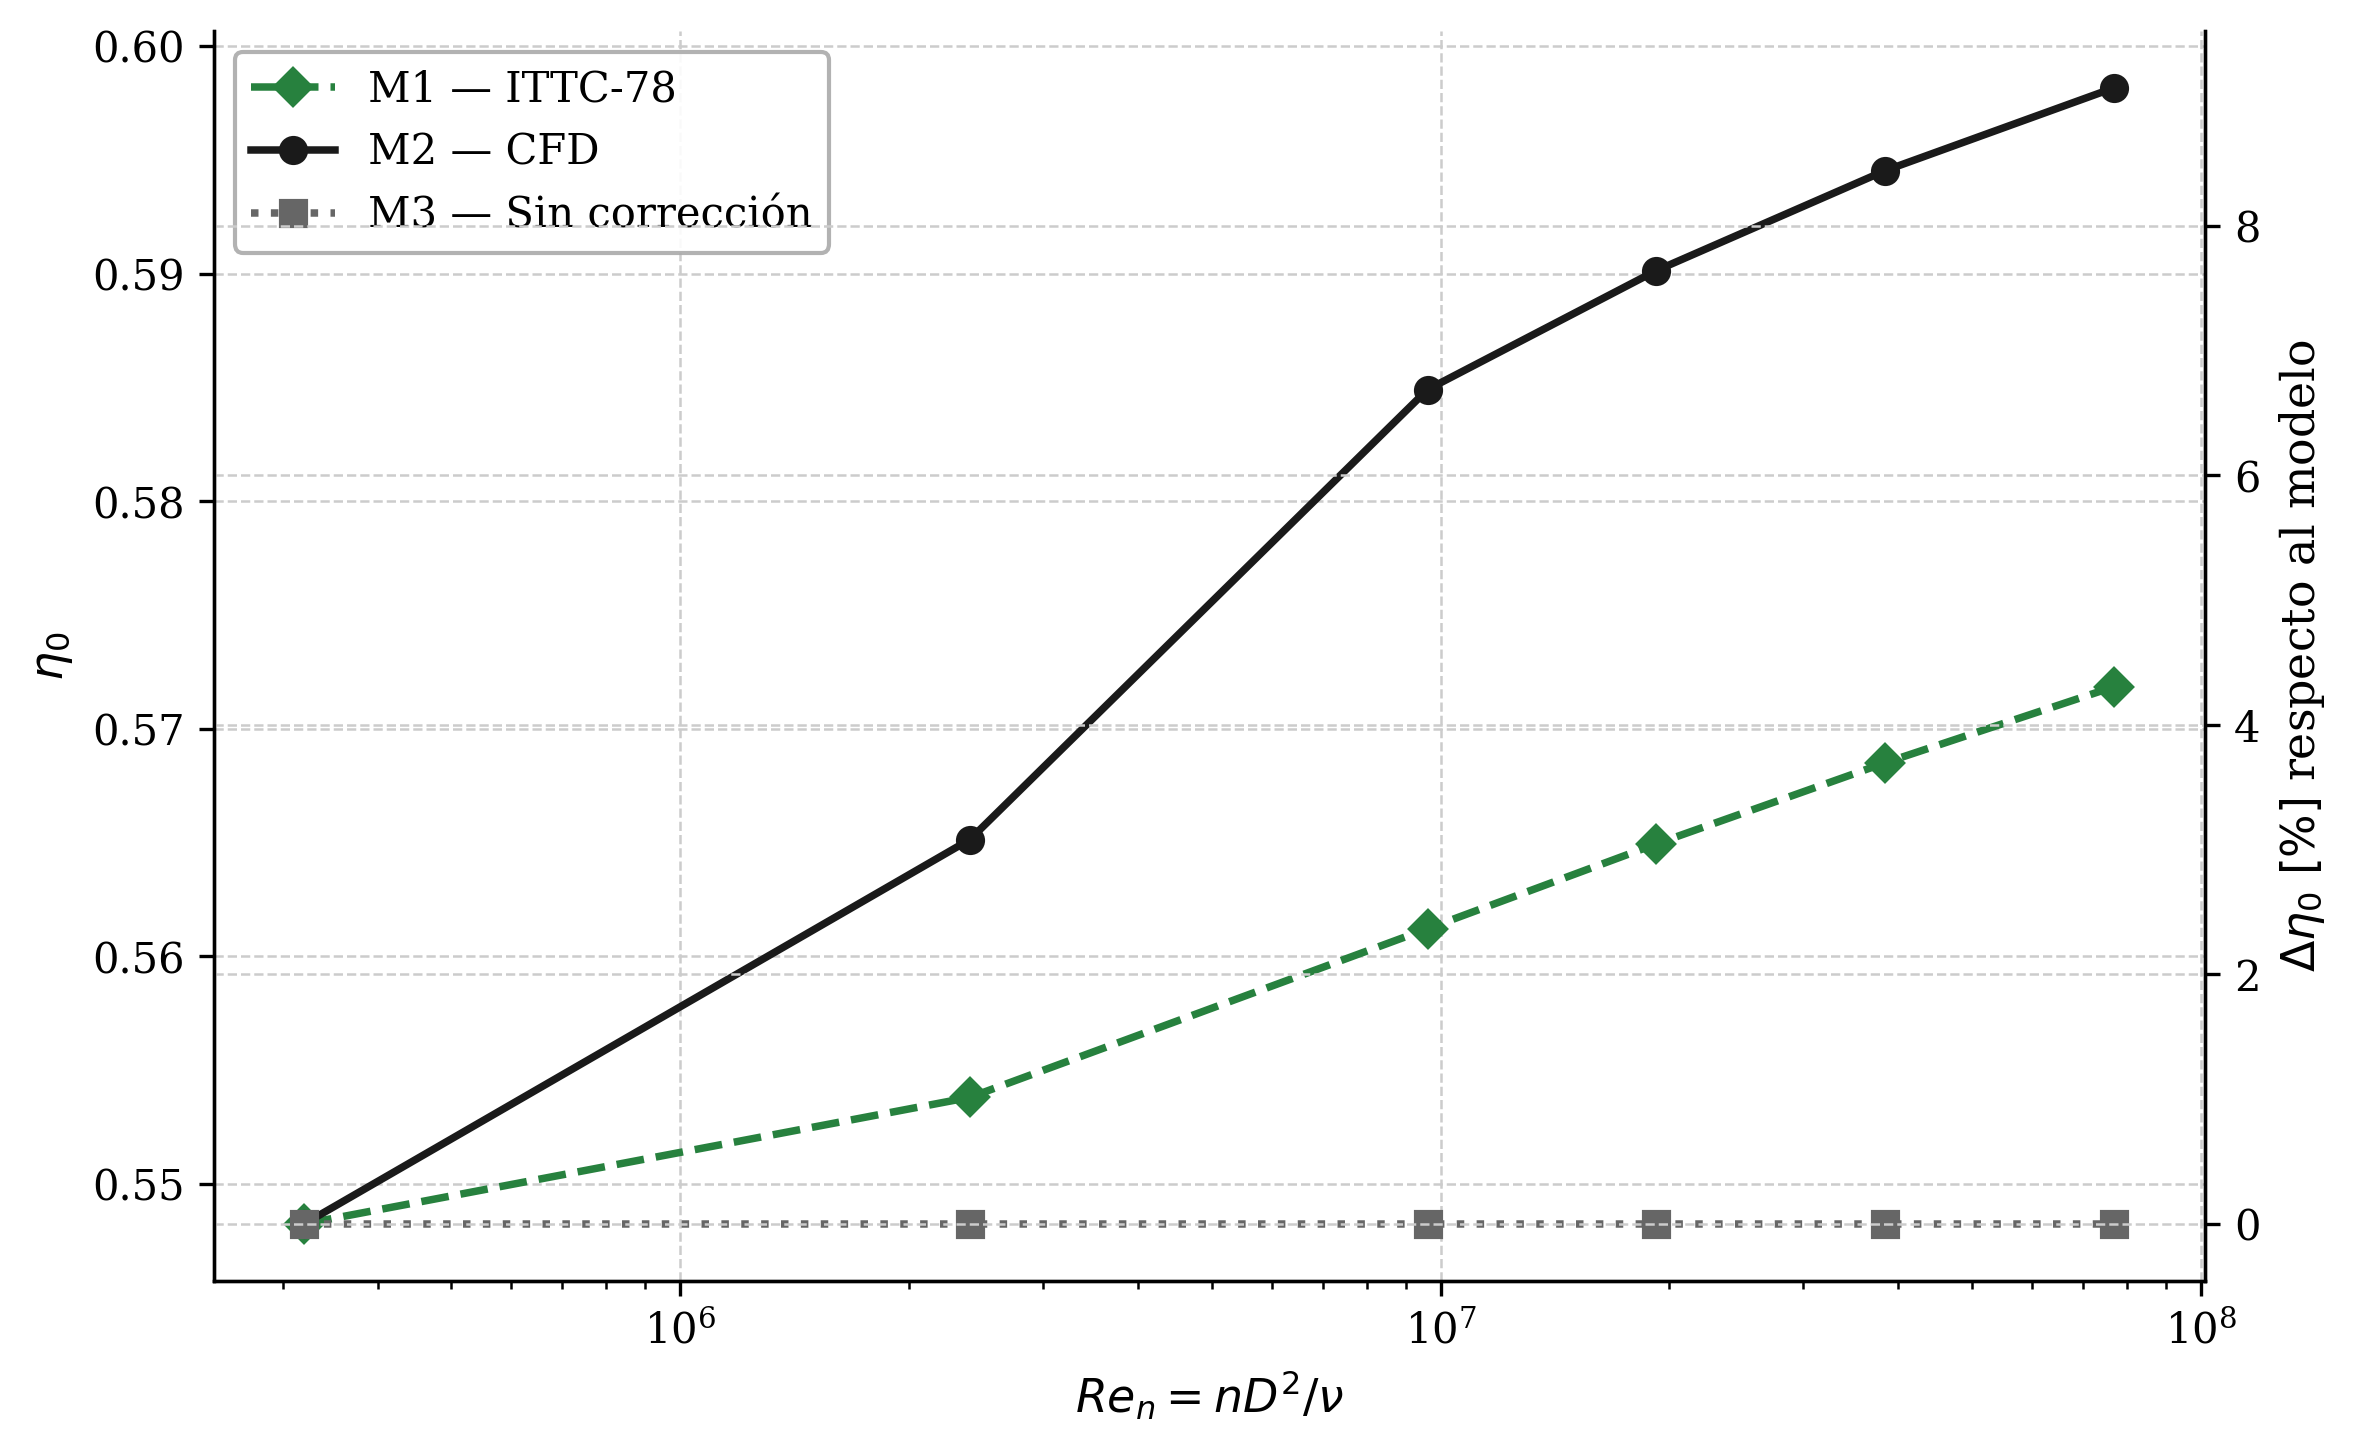
\includegraphics[width=0.95\textwidth]{images/fig2b_eficiencia.png}
\caption{Eficiencia en aguas abiertas $\eta_0$ (izquierda) y variación porcentual $\Delta\eta_0$ respecto al modelo (derecha) en función de $Re_n$, para los métodos ITTC-78 (M1), CFD SST (M2) y sin corrección (M3). Hélice B4-60, $J = 0.5$.}
\label{fig:eficiencia_metodos}
\end{figure}



\subsection{Conclusiones parciales}

El barrido de escala de la hélice B4-60, realizado en régimen completamente
turbulento entre $D=0.14$ y $8.0$~m, muestra que el efecto de escala sobre sus
coeficientes hidrodinámicos no es de naturaleza puramente friccional. El empuje crece
de forma monótona con el número de Reynolds ($\Delta K_T=+4.7\%$) y el par disminuye
($-4.1\%$), lo que se traduce en una ganancia de eficiencia en aguas abiertas de
$+9.1\%$ a la mayor escala (Secciones~\ref{sec:helices_sweep}
y~\ref{sec:helices_kt_kq_re}). La descomposición directa de fuerzas revela que ese
aumento de empuje está dominado por la presión: la fracción $\Delta K_{Tp}/\Delta K_T$
se estabiliza en torno al $76$--$77\%$ para $D\geq1$~m
(Sección~\ref{sec:helices_descomposicion}), de modo que apenas una cuarta parte del
efecto proviene de la reducción de fricción.

El empuje y el par se comportan, sin embargo, de manera asimétrica. Mientras la
componente de presión gobierna el efecto de escala sobre $K_T$, la reducción de par
está dominada por la fricción --$\Delta K_{Qf}$ es negativo y de mayor magnitud que el
pequeño $\Delta K_{Qp}$ positivo--. Esta asimetría explica por qué el procedimiento
ITTC-78, que supone $\Delta K_{Tp}=0$, falla de forma distinta en cada coeficiente:
subestima $K_T$ en $+4.7\%$ pero difiere en $K_Q$ solo un $-1.0\%$, donde las
contribuciones friccional y de presión se compensan parcialmente
(Sección~\ref{sec:helices_ittc78}).

El efecto acumulado sobre la eficiencia es la consecuencia práctica más relevante: el
ITTC-78 predice una ganancia de apenas $+1.1\%$ frente al $+9.1\%$ del CFD, una brecha
de $8.0$ puntos porcentuales a la mayor escala analizada (Sección~\ref{sec:helices_eficiencia}) que
corresponde íntegramente a la contribución de presión que la corrección de placa plana
ignora. Aun para una hélice convencional de área expandida moderada como la B4-60, el
procedimiento clásico subestima así la ganancia de eficiencia a escala buque, con un
sesgo conservador pero no despreciable para el dimensionamiento de la instalación
propulsora.

% ============================================================
%  Sección 5.4: Efectos transicionales: propulsor P206
% ============================================================

\section{Efectos de transición laminar-turbulenta: propulsor P206}
\label{sec:helice_coreana}

El análisis de la hélice Wageningen B4-60 presentado en la sección anterior se realizó
íntegramente con el modelo SST en régimen completamente turbulento, lo cual es apropiado
para el barrido de escalas donde los diámetros de interés operan a números de Reynolds
suficientemente elevados. Sin embargo, a escala de modelo la capa límite sobre el álabe
puede contener regiones laminares de extensión significativa, y su tratamiento numérico
requiere modelos capaces de reproducir la transición laminar-turbulenta. Esta sección
aborda ese problema a través del análisis de una hélice de cuatro álabes, cuyas
características geométricas principales se resumen en la
Tabla~\ref{tab:geom_coreana}.

\subsection{Datos experimentales y rango de Reynolds}
\label{sec:coreana_efd}

Los datos experimentales utilizados como referencia fueron obtenidos en túnel de
cavitación por los fabricantes de la hélice. La campaña experimental completa cubre un
rango de $J$ más amplio; de ella se extrajeron los cinco coeficientes de avance
comparables con el barrido CFD de este trabajo, $J = 0.30$, $0.35$, $0.40$, $0.50$ y
$0.60$, para cinco velocidades de rotación: 10.33,
15.00, 22.50, 29.17 y 36.33~rps, con una densidad del agua de
$\rho = 997.77$~kg/m$^3$ y viscosidad cinemática
$\nu = 0.9565 \times 10^{-6}$~m$^2$/s a 22~°C.

El número de Reynolds se define aquí a partir de la cuerda local a $r/R = 0.7$ y de
la velocidad resultante en esa sección:

\begin{equation}
    Re_c = \frac{V_\text{ref} \, c_{0.7R}}{\nu},
    \qquad
    V_\text{ref} = \sqrt{V_a^2 + (\pi n \cdot 0.7D)^2},
    \label{eq:Re_c}
\end{equation}

donde $V_a = J n D$ es la velocidad de avance. Con la cuerda estimada
$c_{0.7R} \approx 0.234\,D = 58.5$~mm, el rango de $Re_c$ explorado
experimentalmente a $J = 0.5$ es
$[0.36,\,0.52,\,0.77,\,1.00,\,1.25] \times 10^6$, abarcando desde el régimen
claramente subcrítico hasta valores próximos al umbral de turbulencia plena para
perfiles de álabe marino.

Este rango resulta especialmente relevante porque contiene la denominada
``joroba'': la región de Reynolds en torno a
$Re_c \sim 5 \times 10^5$ donde la capa límite experimenta la transición
laminar-turbulenta y las fuerzas sobre el álabe exhiben un comportamiento
no monótono, con un incremento local de $K_T$ y $10K_Q$ que ningún modelo
completamente turbulento es capaz de reproducir.

\subsection{Configuración numérica}
\label{sec:coreana_cfd}

Las simulaciones propias se realizaron con OpenFOAM, siguiendo la
metodología general descripta en la Sección~\ref{sec:metodologia_helices} --incluido el
dominio reducido de $90^\circ$ de la Figura~\ref{fg:helice_dominio}--, con los
dos modelos de turbulencia allí presentados (SST completamente turbulento y SST-LM).
Estos resultados se contrastan con los obtenidos en StarCCM+ por S.~Gaggero sobre la
misma geometría, provistos para este trabajo como verificación cruzada entre códigos.
A continuación se detallan únicamente los parámetros específicos de este caso.

Las simulaciones en StarCCM+ (S.~Gaggero) se realizaron a las mismas velocidades de giro que los
ensayos experimentales (10.33 a 36.33~rps), con densidad $\rho = 998.71$~kg/m$^3$ y
viscosidad $\nu = 1.0034 \times 10^{-6}$~m$^2$/s a 20~°C.

En la malla de OpenFOAM se emplearon 10 capas de prismas sobre la superficie del
álabe para resolver la capa límite bajo el criterio de $y^+$ descripto en la
Sección~\ref{sec:metodologia_helices_openfoam}. La malla resultante cuenta con
$4\,935\,785$ celdas.

En ambos códigos, las simulaciones con SST-LM se realizaron para tres niveles de
intensidad turbulenta efectiva en el plano del disco: $Tu = 1.0\%$, $1.4\%$ y
$1.8\%$, siguiendo el procedimiento de calibración descripto en la
Sección~\ref{sec:metodologia_helices_tu}.

\subsection{Sensibilidad a la intensidad turbulenta y comparación con datos
experimentales}
\label{sec:coreana_resultados}

La Figura~\ref{fig:coreana_KT_OF} presenta el coeficiente $K_T$ y la
Figura~\ref{fig:coreana_KQ_OF} el coeficiente $10K_Q$, ambos en función del número de
Reynolds $Re_c$ para $J = 0.3$, $0.4$, $0.5$ y $0.6$, obtenidos con OpenFOAM y
comparando las predicciones del modelo SST completamente turbulento, las tres
configuraciones SST-LM y los datos experimentales. La comparación equivalente con
StarCCM se presenta en la Sección~\ref{sec:coreana_solvers}.

\begin{figure}[htpb]
    \centering
    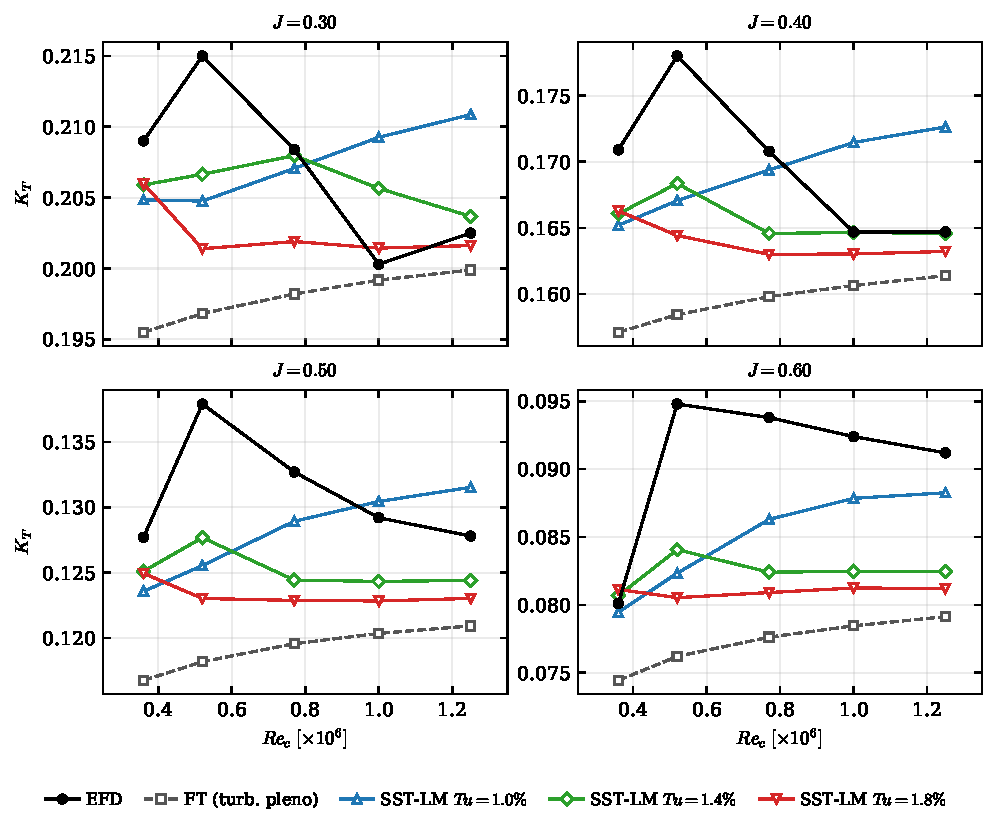
\includegraphics[width=\textwidth]{fig_coreana_KT_OF.pdf}
    \caption{Coeficiente de empuje $K_T$ en función de $Re_c$ para cuatro valores de
    $J$, calculado con \textbf{OpenFOAM}. Comparación entre el modelo SST completamente
    turbulento, el modelo SST-LM con $Tu = 1.0\%$, $1.4\%$ y $1.8\%$ en el disco, y los
    datos experimentales.}
    \label{fig:coreana_KT_OF}
\end{figure}

\begin{figure}[htpb]
    \centering
    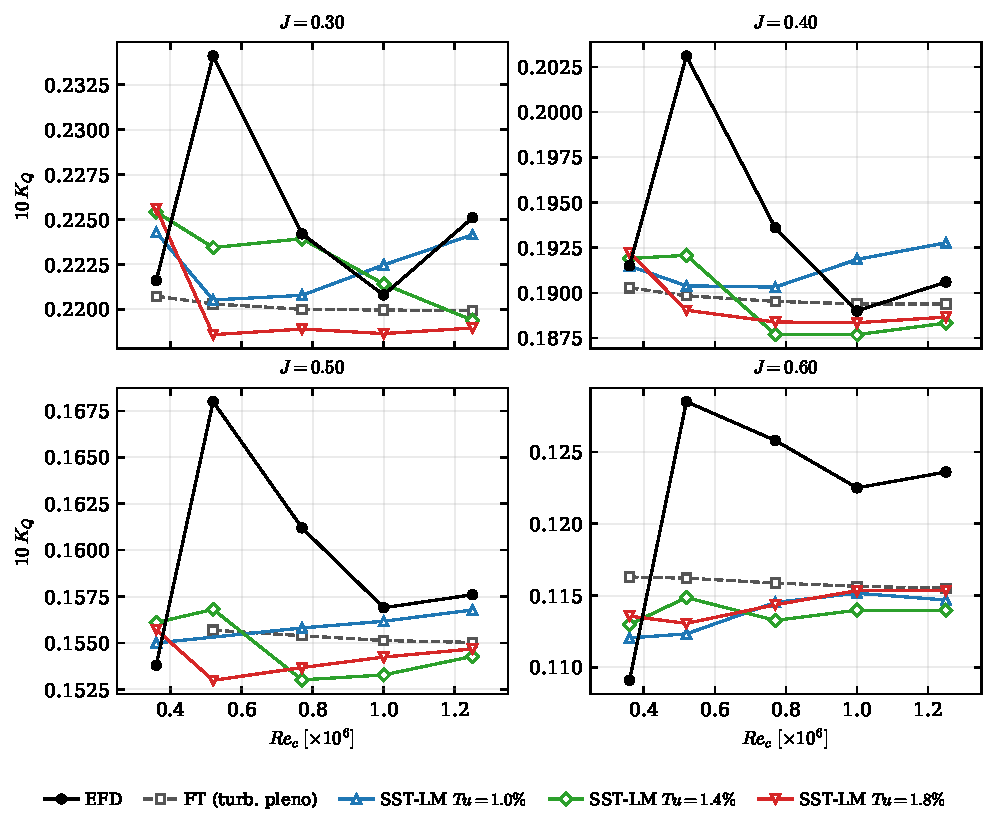
\includegraphics[width=\textwidth]{fig_coreana_KQ_OF.pdf}
    \caption{Coeficiente de par $10K_Q$ en función de $Re_c$ para cuatro valores de
    $J$, calculado con \textbf{OpenFOAM}. Configuraciones análogas a las de la
    Figura~\ref{fig:coreana_KT_OF}.}
    \label{fig:coreana_KQ_OF}
\end{figure}

El modelo SST completamente turbulento predice coeficientes poco sensibles al
$Re_c$: tanto $K_T$ como $10K_Q$ exhiben un crecimiento monótono leve en todo el rango
de velocidades de rotación ensayado --del $2$--$3\%$ en las condiciones cargadas
($J\leq0.40$) y de hasta un $6\%$ en las descargadas ($J=0.60$), entre el menor y el
mayor $Re_c$ de modelo--. Este comportamiento es esperado, ya que el modelo no tiene
mecanismo para distinguir entre una capa límite laminar y una turbulenta; la variación
que sí predice proviene únicamente del cambio de viscosidad efectiva con el número de
Reynolds.

Los resultados con SST-LM exhiben un comportamiento cualitativamente distinto: para
los Reynolds más bajos ($Re_c \leq 5 \times 10^5$) el modelo predice valores de
$K_T$ superiores a los del SST --y, en la mayoría de las condiciones, también de
$10K_Q$, aunque en algunos puntos el par del SST resulta mayor--, mientras que para
Reynolds elevados ($Re_c \geq 10^6$) ambos modelos tienden a converger, con la
excepción de la configuración $Tu = 1.0\%$, que conserva una región laminar apreciable
y mantiene una diferencia con el SST incluso en el extremo superior del rango. Este
incremento a bajo $Re_c$ es precisamente la manifestación de la ``joroba
transicional'': la presencia de flujo laminar sobre una fracción significativa del
álabe reorienta las líneas de corriente de la capa límite en sentido más radial y
altera la carga a lo largo de la envergadura, modificando la distribución de presión
sobre el álabe. Este es el mecanismo que \citet{rijpkema2015viscous} infirió de los
ensayos de ``paint test'', y que eleva tanto el empuje como el par respecto del caso
completamente turbulento, en concordancia con lo reportado por \citet{Gaggero2020}
para la VP1304 y \citet{Baltazar2021} para la S6368. Conviene anticipar --y se
demuestra en la Sección~\ref{sec:coreana_diagnostico}-- que esta modificación de la
presión \emph{no} se produce por un aumento del pico de succión, que resulta
insensible al modelo de turbulencia, sino por una redistribución de la carga en otras
zonas del álabe.

La intensidad turbulenta en el disco actúa como parámetro de ajuste del punto de
inicio de la transición: a mayor $Tu$, la transición se adelanta hacia el borde de
ataque y la región laminar se reduce, aproximando el resultado al caso completamente
turbulento. En consecuencia, la configuración $Tu = 1.8\%$ produce la joroba menos
pronunciada, mientras que $Tu = 1.0\%$ maximiza la extensión de flujo laminar y
amplifica las diferencias con respecto al SST.

La comparación con los datos experimentales permite identificar cuál de las
configuraciones SST-LM representa mejor las condiciones reales del túnel de
cavitación. Los ensayos muestran claramente la presencia de la joroba: los
coeficientes experimentales son notoriamente superiores a los predichos por el SST a
$Re_c$ bajos y se acercan a él a medida que $Re_c$ crece, confirmando que la capa
límite del modelo opera en régimen de transición en el rango ensayado. Esa aproximación
no llega a cerrarse dentro del rango de $Re_c$ ensayado: es prácticamente completa a
$J\leq0.40$ (brecha residual de $0.6$--$2.5\%$ en el mayor $Re_c$ disponible), pero a
$J=0.50$--$0.60$ persiste una diferencia apreciable de $5$ a $24\%$ incluso en ese
punto; que el SST completamente turbulento y el ensayo terminen de converger a
Reynolds aún mayores es, en esas condiciones, una expectativa razonable pero no
verificada con los datos disponibles. La
configuración SST-LM con $Tu = 1.4\%$ ofrece en general el mejor acuerdo cuantitativo
con los datos, mientras que $Tu = 1.0\%$ tiende a sobreestimar el efecto transicional
y $Tu = 1.8\%$ lo subestima.

Cuantitativamente, la amplitud de la joroba experimental --medida como la diferencia
relativa entre el $K_T$ del máximo y el del extremo de mayor $Re_c$-- crece con la
descarga del propulsor, desde un $7.1\%$ a $J=0.30$ hasta un $16.3\%$ a $J=0.60$, con
el máximo ubicado consistentemente en $Re_c = 0.52\times10^6$. El modelo SST-LM genera
no-monotonía en cuatro a cinco de las seis combinaciones solver-$Tu$ según el $J$, pero
en el mejor de los casos reproduce una amplitud de $3.4\%$ a $J=0.30$ y $10.4\%$ a
$J=0.60$ --aproximadamente la mitad de la amplitud experimental--, y solo combinaciones aisladas ubican
el máximo en $Re_c = 0.52\times10^6$, ninguna de ellas de forma consistente para todos
los $J$. Esta reproducción parcial es la que hace necesario el ejercicio de calibración
de $Tu$ que sigue, y anticipa su resultado: como ningún $Tu$ único reproduce la forma de
la curva, el nivel que mejor ajusta los datos necesariamente cambia de una condición de
operación a otra.

A diferencia del efecto de escala de la B4-60 (Sección~\ref{sec:helices_descomposicion}),
el desfasaje que introduce la transición se cuantifica aquí como la diferencia, a igual
$Re_c$ y $J$, entre la solución SST-LM y la completamente turbulenta,
$\delta K_{Ti} = K_{Ti}^{\mathrm{LM}} - K_{Ti}^{\mathrm{FT}}$ con $i\in\{p,f\}$ (se emplea
$\delta$ para distinguirla de la corrección de extrapolación $\Delta$). La descomposición
de fuerzas en componentes de presión y fricción (Ecuación~\ref{eq:adim_helices}) está
disponible para ambos modelos en OpenFOAM, de modo que el origen del desfasaje puede
leerse de forma directa. Al incluir la transición, la diferencia de empuje respecto del
caso completamente turbulento proviene mayoritariamente de la presión --del orden del
$90\%$ (Tabla~\ref{tab:coreana_decomp})--, y la fricción aporta el resto menor en el mismo sentido: el exceso de empuje no
es un efecto friccional. En el par, en cambio, las contribuciones de presión y fricción
se oponen: la parte friccional disminuye, como cabría esperar de una reducción del
arrastre viscoso, mientras que la de presión aumenta y la compensa en gran medida, de
modo que $K_Q$ varía poco (una leve alza de $+0.6$ a $+1.6\%$ a $J = 0.30$--$0.40$). Como
$\delta K_{Qp}$ y $\delta K_{Qf}$ son de magnitud similar y signo opuesto, su diferencia
$\delta K_Q$ es pequeña, y una fracción de presión análoga a la del efecto de escala no
resulta significativa para el par. Esta composición se mantiene al variar el nivel de
$Tu$ del modelo de transición, por lo que el origen de presión del exceso de empuje y la
cancelación mutua en el par son propiedades del régimen transicional y no de una
calibración particular. Ambos hechos reproducen, para esta hélice, el comportamiento
reportado por \citet{gaggero2018transition}: el mecanismo transicional no se limita a la
fricción, sino que arrastra una contribución de presión, en consonancia con lo hallado en
la Sección~\ref{sec:helices_escala} para la B4-60.

\begin{table}[htpb]
\centering
\footnotesize
\caption{Descomposición presión/fricción de la diferencia respecto del modelo
completamente turbulento ($\delta K_{Ti} = K_{Ti}^{\mathrm{LM}} - K_{Ti}^{\mathrm{FT}}$,
SST-LM a $Tu = 1.0\%$ frente al FT a igual $Re_c$ y $J$), para puntos representativos en
los dos $Re_c$ extremos de la campaña.}
\label{tab:coreana_decomp}
\begin{tabular}{cccccc}
\hline
$Re_c$~[$\times10^6$] & $J$ & $\delta K_T$~[\%] & $\delta K_{Tp}/\delta K_T$~[\%] & $\delta K_{Qp}$ & $\delta K_{Qf}$ \\
\hline
$0.36$ & $0.30$ & $+4.8$  & $91$ & $+0.0013$ & $-0.0010$ \\
$1.25$ & $0.30$ & $+5.5$  & $93$ & $+0.0013$ & $-0.0009$ \\
$0.36$ & $0.60$ & $+6.8$  & $79$ & $+0.0006$ & $-0.0011$ \\
$1.25$ & $0.60$ & $+11.5$ & $89$ & $+0.0010$ & $-0.0011$ \\
\hline
\end{tabular}
\end{table}

\subsection{Diagnóstico seccional: dónde actúan la presión y la fricción}
\label{sec:coreana_diagnostico}

Para localizar sobre el álabe el cambio de presión implicado por la descomposición anterior
se analizaron los coeficientes locales $C_{pn}$ y $C_f$ (Ecuación~\ref{eq:cpn_cf_def})
sobre el dorso del álabe, en cuatro radios ($r/R = 0.3$ a $0.9$, a $J = 0.5$ y para
los dos $Re_c$ extremos). El resultado acota el problema en sentido negativo: el pico
de $C_{pn}$ es prácticamente insensible al modelo de turbulencia --la dispersión entre
el completamente turbulento y los tres niveles de $Tu$ se mantiene por debajo del
$3.1\%$ en todos los radios--, de modo que el cambio de presión \emph{no} se produce
por un desplazamiento del pico de succión y debe originarse en una redistribución de
la carga en otras zonas (extensión en cuerda, carga sobre la cara de presión o región
de punta); el pico es un valor puntual, mientras que $K_{Tp}$ es la integral de
superficie de $p\,n_x$.

El coeficiente $C_f$, en cambio, separa nítidamente las configuraciones: el
completamente turbulento predice los valores más altos y el crecimiento más rápido
hacia la punta. A $Re_c$ elevado, los niveles $Tu = 1.4\%$ y $1.8\%$ muestran un
frente de transición marcado --un salto entre la zona de $C_f$ bajo y la de $C_f$
alto-- cuya posición depende de $Tu$, mientras que $Tu = 1.0\%$ mantiene flujo
predominantemente laminar sobre casi todo el álabe; a $Re_c$ bajo los tres niveles se
comportan de forma similar. La dirección de la tensión de corte es visiblemente más
radial en las regiones laminares: la fracción radial de $|\tau_w|$ --el cociente entre
la componente radial de la tensión de corte en la pared y su módulo, promediado sobre
el álabe-- aumenta de $0.19$ en el caso completamente turbulento a $0.40$--$0.43$ en el
SST-LM a $Re_c$ bajo. Esta
reorientación es la que altera la carga a lo largo de la envergadura --el mecanismo
inferido por \citet{rijpkema2015viscous} de los ``paint tests''-- y constituye la vía
plausible por la cual la transición modifica el campo de presión --a través de esa
redistribución de carga a lo largo de la envergadura-- sin alterar el pico de succión,
que permanece insensible al modelo.

% ============================================================
%  Figura del panel Cf sobre la pala (5 Re_c x 4 niveles de Tu).
%  Generada con cf_panel_5Re.py -> fig_cf_panel.png
%  PENDIENTE: confirmar que el render final usa los VTK ya depurados
%  (ver auditoria de casos FT/Tu1.0 contaminados) antes de dar por
%  cerrada la interpretacion cuantitativa del texto que sigue.
% ============================================================
\begin{figure}[htpb]
\centering
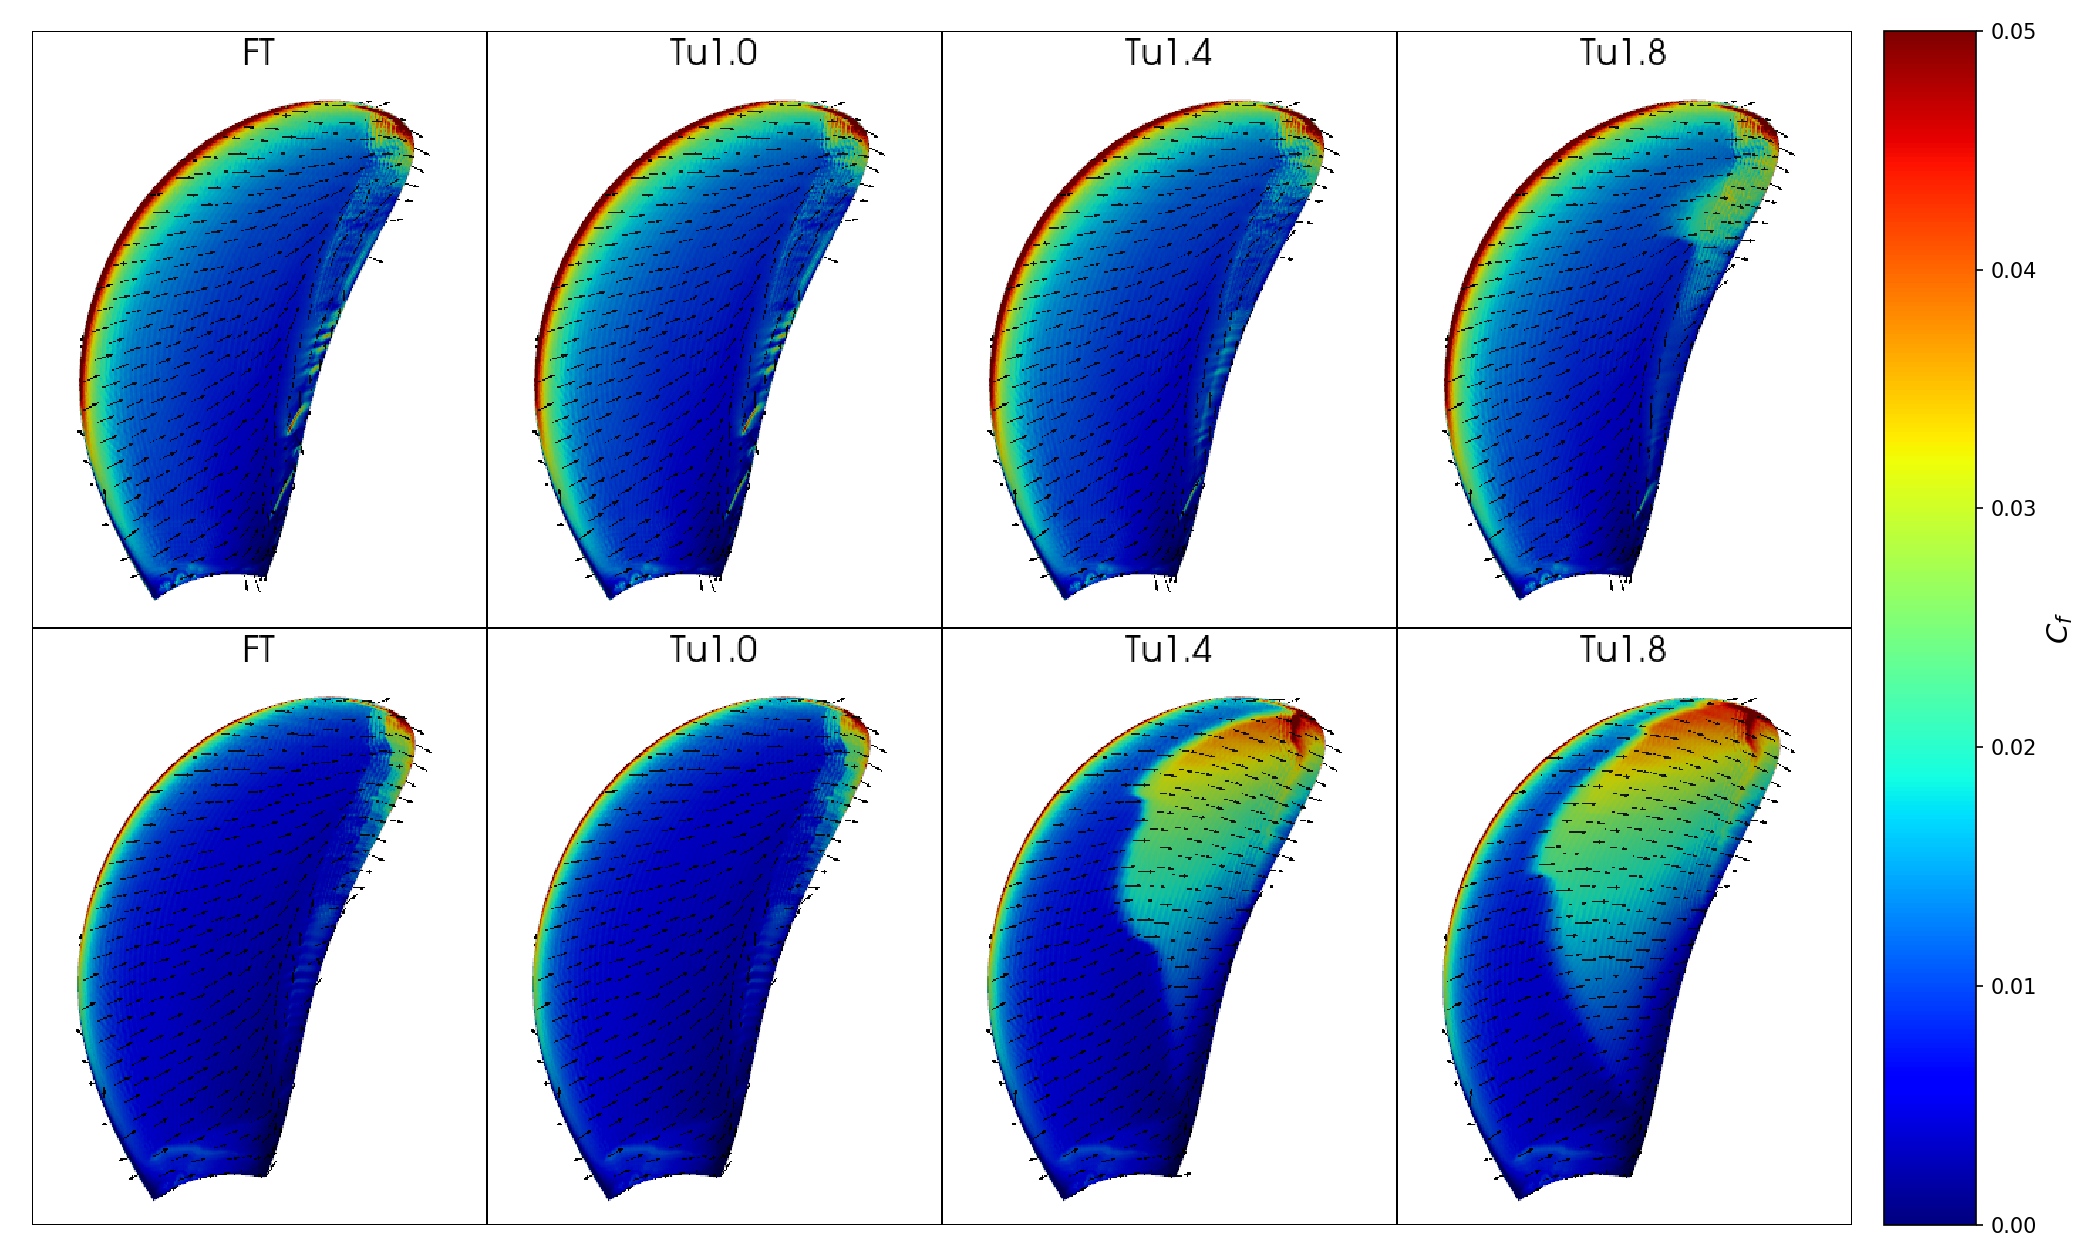
\includegraphics[width=0.85\textwidth]{fig_cf_panel.png}
\caption{Distribución espacial de $C_f$ sobre el dorso del álabe, para $J=0.5$, los
cinco $Re_c$ ensayados (filas, de $0.36$ a $1.25\times10^6$) y los cuatro niveles de
turbulencia (columnas: completamente turbulento y $Tu=1.0\%$, $1.4\%$, $1.8\%$). Las
flechas indican la dirección local de la tensión de corte.}
\label{fig:coreana_cf_panel}
\end{figure}

La Figura~\ref{fig:coreana_cf_panel} ilustra directamente lo descripto en el párrafo
anterior: el frente de transición --visible como el salto entre la zona azul ($C_f$
bajo) y la zona roja ($C_f$ alto)-- se desplaza hacia el borde de ataque a medida que
$Tu$ y $Re_c$ aumentan, y las flechas evidencian la reorientación radial de la tensión
de corte en las regiones aún laminares.

En síntesis, la transición se manifiesta de forma \emph{local} y nítida en el campo de fricción
--el frente de transición y su sensibilidad a $Tu$ y $Re_c$--, mientras que el cambio
acompañante en el empuje de presión integrado, dominante según el argumento de
magnitud, no está localizado en el pico de succión y queda pendiente de resolver en
detalle; cerrarlo requeriría aplicar la descomposición de la
Ecuación~\ref{eq:adim_helices} a las corridas SST-LM, disponible aquí solo para las
configuraciones completamente turbulentas.

Estos resultados subrayan que el modelo SST, al imponer turbulencia plena desde el
borde de ataque, es incapaz de reproducir el comportamiento experimental en la escala
de modelo para esta hélice. La elección del modelo de turbulencia no es, por tanto,
un detalle numérico menor: condiciona de manera fundamental la validez de las
predicciones a escala de modelo y, en consecuencia, la confiabilidad del proceso de
extrapolación a escala buque.

\subsection{Comparación entre solvers: robustez de la calibración de $Tu$}
\label{sec:coreana_solvers}

La disponibilidad de resultados equivalentes en StarCCM+ y OpenFOAM para las mismas
ocho combinaciones de modelo de turbulencia (Fully Turbulent y SST-LM con
$Tu = 1.0\%$, $1.4\%$ y $1.8\%$, en cada código) permite evaluar no solo qué
configuración predice mejor $K_T$, sino también cuán sensible es esa conclusión a la
elección del solver. Las Figuras~\ref{fig:coreana_KT_Star} y \ref{fig:coreana_KQ_Star}
reproducen, para StarCCM+, las mismas curvas que las Figuras~\ref{fig:coreana_KT_OF}
y \ref{fig:coreana_KQ_OF} mostraban para OpenFOAM. La comparación directa entre ambos
códigos revela una diferencia cualitativa relevante: mientras que en OpenFOAM las
configuraciones SST-LM tienden a producir curvas monótonas que se aproximan
gradualmente a la joroba experimental sin reproducir su forma, en StarCCM+ las mismas
configuraciones exhiben una no-monotonía marcada, con un máximo local próximo al
$Re_c \approx 0.52\times10^6$ del experimento. Es decir, el mismo modelo de transición,
alimentado con el mismo $Tu$ en el disco, produce comportamientos cuantitativamente
--y en parte cualitativamente-- distintos según el solver, lo que anticipa la
conclusión sobre la no transferibilidad del parámetro entre códigos.

\begin{figure}[htpb]
    \centering
    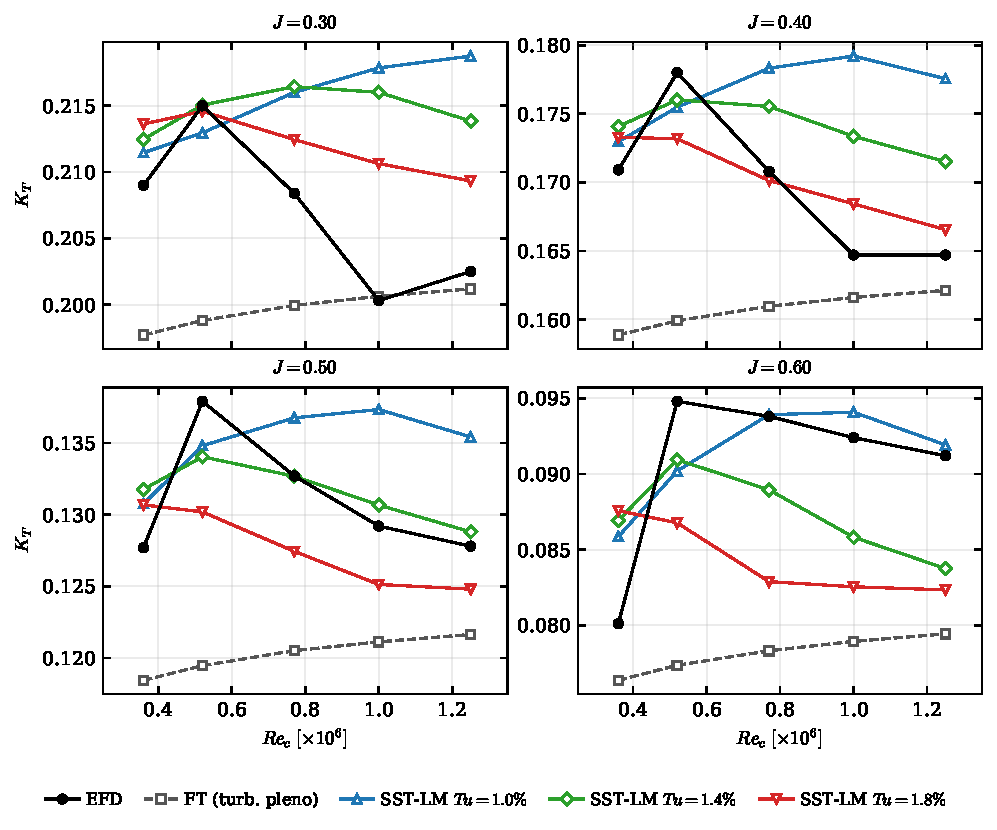
\includegraphics[width=\textwidth]{fig_coreana_KT_Star.pdf}
    \caption{Coeficiente de empuje $K_T$ en función de $Re_c$ para cuatro valores de
    $J$, calculado con \textbf{StarCCM+}. Configuraciones análogas a las de la
    Figura~\ref{fig:coreana_KT_OF}.}
    \label{fig:coreana_KT_Star}
\end{figure}

\begin{figure}[htpb]
    \centering
    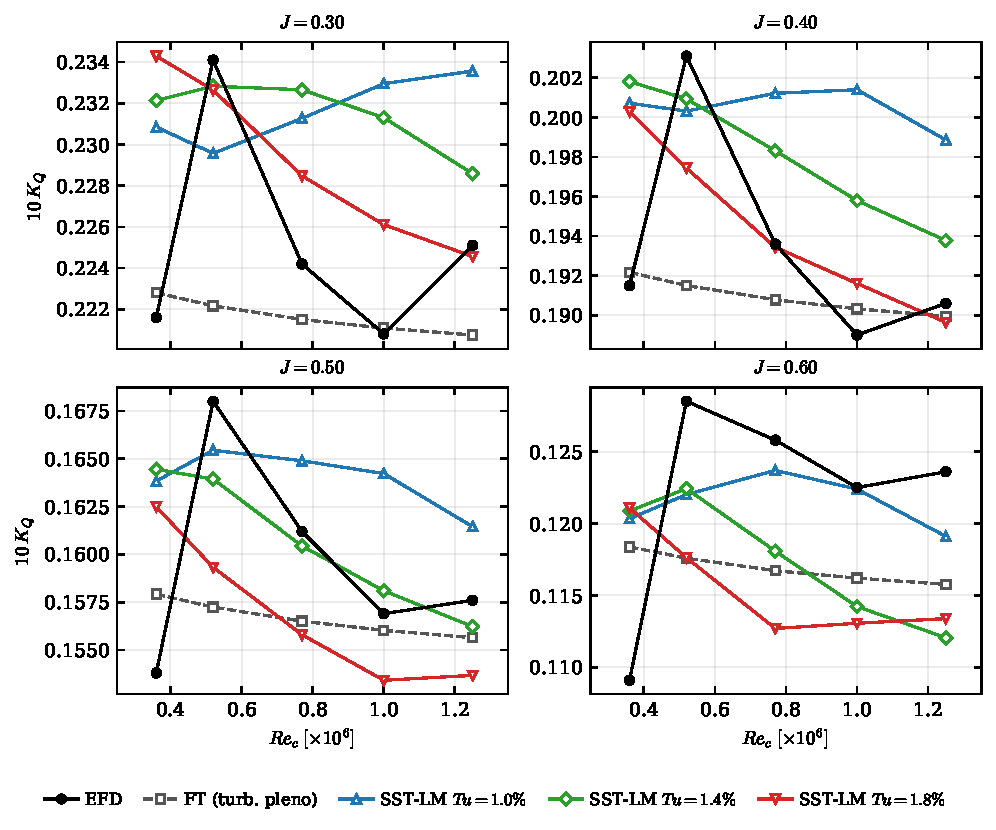
\includegraphics[width=\textwidth]{fig_coreana_KQ_Star.pdf}
    \caption{Coeficiente de par $10K_Q$ en función de $Re_c$ para cuatro valores de
    $J$, calculado con \textbf{StarCCM+}. Configuraciones análogas a las de la
    Figura~\ref{fig:coreana_KT_OF}.}
    \label{fig:coreana_KQ_Star}
\end{figure}

Para cuantificar el acuerdo con el experimento se emplean dos métricas relativas.
Sean $K_i^{\mathrm{CFD}}$ el valor calculado y $K_i^{\mathrm{EFD}}$ el experimental en
el punto de operación $i$ ($i=1,\dots,N$); el error absoluto medio (MAE) y el sesgo
(\emph{bias}) se definen, en porcentaje, como
%
\begin{equation}
\mathrm{MAE} = \frac{100}{N}\sum_{i=1}^{N}
\frac{\bigl|K_i^{\mathrm{CFD}}-K_i^{\mathrm{EFD}}\bigr|}{K_i^{\mathrm{EFD}}},
\qquad
\mathrm{sesgo} = \frac{100}{N}\sum_{i=1}^{N}
\frac{K_i^{\mathrm{CFD}}-K_i^{\mathrm{EFD}}}{K_i^{\mathrm{EFD}}}.
\label{eq:mae_bias}
\end{equation}
%
El MAE mide la magnitud típica del desvío (siempre positivo) y el sesgo su signo
--negativo si el modelo subestima, positivo si sobreestima--; ambos coinciden en valor
absoluto cuando el error tiene el mismo signo en todos los puntos. La
Tabla~\ref{tab:mae_global_coreana} resume el MAE y el sesgo de $K_T$ de las ocho
configuraciones de solver/modelo frente a los $N=25$ puntos experimentales
($J=0.30$--$0.60$; cinco $Re_c$ por cinco $J$).

\begin{table}[htpb]
\centering
\caption{Error absoluto medio (MAE) y sesgo de $K_T$ respecto de los datos
experimentales (Ecuación~\ref{eq:mae_bias}), para las ocho configuraciones de
solver/modelo de turbulencia evaluadas.}
\label{tab:mae_global_coreana}
\begin{tabular}{clccc}
\hline
Ranking & Configuración & $N$ & MAE~[\%] & Bias~[\%] \\
\hline
1 & StarCCM+, $Tu = 1.4\%$      & 25 & 3.51 & $+1.18$ \\
2 & StarCCM+, $Tu = 1.8\%$      & 25 & 3.82 & $-1.30$ \\
3 & OpenFOAM, $Tu = 1.4\%$      & 25 & 3.91 & $-3.49$ \\
4 & OpenFOAM, $Tu = 1.0\%$      & 25 & 4.05 & $-1.63$ \\
5 & StarCCM+, $Tu = 1.0\%$      & 25 & 4.20 & $+3.34$ \\
6 & OpenFOAM, $Tu = 1.8\%$      & 25 & 4.95 & $-4.79$ \\
7 & StarCCM+, Fully Turbulent   & 25 & 6.95 & $-6.93$ \\
8 & OpenFOAM, Fully Turbulent   & 25 & 7.76 & $-7.76$ \\
\hline
\end{tabular}
\end{table}

Los cinco primeros puestos del ranking son estadísticamente comparables (MAE entre
$3.5\%$ y $4.2\%$), y las dos configuraciones Fully Turbulent --una por código--
ocupan los dos últimos puestos, lo cual confirma --ahora de manera cuantitativa--
que para esta hélice la elección del modelo de transición pesa más que la elección
del solver. El signo del sesgo, sin embargo, no sigue el mismo patrón en los dos
códigos: OpenFOAM subestima $K_T$ de forma sistemática en las cuatro
configuraciones (bias negativo en todas, de $-1.63$ a $-7.76\%$), mientras que en
StarCCM+ el signo depende del nivel de $Tu$ --$Tu=1.0\%$ y $Tu=1.4\%$ sobreestiman
($+3.34\%$ y $+1.18\%$), pero $Tu=1.8\%$ y Fully Turbulent subestiman ($-1.30\%$ y
$-6.93\%$)--. El nivel de $Tu$ que minimiza el MAE global coincide en ambos
códigos ($Tu=1.4\%$), pero el orden del resto no se transfiere: en OpenFOAM el
segundo mejor es $Tu=1.0\%$ y el peor $Tu=1.8\%$, mientras que en StarCCM+ el
segundo mejor es $Tu=1.8\%$ y el peor $Tu=1.0\%$ --el extremo opuesto--, lo que
indica que el ajuste fino del parámetro no es transferible entre solvers sin
recalibración, incluso cuando el óptimo global coincide.

Esta no transferibilidad se manifiesta con más claridad todavía dentro de cada
código si se examina, punto a punto, cuál es el $Tu$ que minimiza el error en cada
combinación de $Re_c$ y $J$, en lugar del promedio global. El $Tu$ óptimo no es
constante: sigue una tendencia sistemática con la carga del propulsor, favoreciendo
los niveles bajos ($Tu=1.0\%$) en la condición más descargada ($J=0.60$) y los
niveles altos ($Tu=1.4\%$--$1.8\%$) en las cargadas. Más aún, el $Tu$ óptimo punto a
punto coincide entre los dos solvers en solo 11 de los 25 puntos experimentales
($44\%$) --pese a que ambos códigos acuerdan en el óptimo \emph{global}--. En
conjunto, esto confirma que la intensidad turbulenta que mejor reproduce los datos
no es una propiedad física transferible del ensayo, sino un parámetro de ajuste que
depende de la condición de operación y del código: una herramienta de validación, no
una constante del problema.

La Tabla~\ref{tab:mae_re_coreana} desagrega el MAE por número de Reynolds. La
condición $Re_c \approx 520\,000$ --la más próxima al centro de la joroba-- concentra
sistemáticamente el mayor error para casi todas las configuraciones, incluyendo las
mejor rankeadas globalmente, lo que confirma que es en el corazón de la transición
donde ambos códigos tienen mayor dificultad para predecir la extensión exacta de la
región laminar.

\begin{table}[htpb]
\centering
\small
\caption{MAE de $K_T$ [\%] por número de Reynolds, para las configuraciones mejor
rankeadas de cada código.}
\label{tab:mae_re_coreana}
\begin{tabular}{lccccc}
\hline
Configuración & $360$k & $520$k & $770$k & $1000$k & $1250$k \\
\hline
OpenFOAM, $Tu=1.4\%$   & 1.79 & 6.50 & 5.01 & 3.66 & 2.62 \\
StarCCM+, $Tu=1.4\%$   & 3.45 & 1.74 & 2.72 & 5.23 & 4.43 \\
StarCCM+, $Tu=1.8\%$   & 3.14 & 4.13 & 3.86 & 4.56 & 3.39 \\
StarCCM+, $Tu=1.0\%$   & 2.68 & 2.16 & 3.05 & 6.90 & 6.22 \\
StarCCM+, Fully Turb.  & 6.14 & 11.65 & 8.06 & 4.70 & 4.18 \\
OpenFOAM, Fully Turb.  & 7.55 & 12.60 & 8.77 & 5.25 & 4.65 \\
\hline
\end{tabular}
\end{table}

La dependencia con la carga del propulsor es igualmente relevante: para la mayoría de
las configuraciones, $J = 0.60$ --próximo al punto de eficiencia máxima de la hélice--
resulta la condición más difícil de predecir, con errores de hasta el $14\%$ en el
caso Fully Turbulent, mientras que las cargas altas ($J \leq 0.40$) presentan el
mejor acuerdo generalizado. Esto sugiere que, a medida que el propulsor se descarga,
la topología de la capa límite laminar sobre el álabe se vuelve más sensible tanto al
modelo de transición como al solver empleado.

Un resultado adicional, de utilidad práctica, surge de comparar el par $K_Q$ frente al
empuje $K_T$. El EFD del fabricante reporta $K_Q$ en las mismas 25 condiciones
utilizadas para $K_T$ ($J=0.30$--$0.60$), y ambos códigos las cubren por completo, de
modo que el MAE de $K_Q$ se computa, para las ocho configuraciones, sobre el mismo
$N=25$ que $K_T$. La Tabla~\ref{tab:mae_kq_coreana} resume el MAE y el sesgo de $K_Q$
(Ecuación~\ref{eq:mae_bias}) de las ocho configuraciones, de forma análoga a la
Tabla~\ref{tab:mae_global_coreana} para $K_T$.

\begin{table}[htpb]
\centering
\caption{Error absoluto medio (MAE) y sesgo de $K_Q$ respecto de los datos
experimentales (Ecuación~\ref{eq:mae_bias}), para las ocho configuraciones de
solver/modelo de turbulencia evaluadas.}
\label{tab:mae_kq_coreana}
\begin{tabular}{clccc}
\hline
Ranking & Configuración & $N$ & MAE~[\%] & Bias~[\%] \\
\hline
1 & StarCCM+, Fully Turbulent   & 25 & 3.01 & $-1.91$ \\
2 & OpenFOAM, $Tu = 1.0\%$      & 25 & 3.23 & $-2.37$ \\
3 & OpenFOAM, Fully Turbulent   & 25 & 3.30 & $-2.63$ \\
4 & OpenFOAM, $Tu = 1.4\%$      & 25 & 3.47 & $-2.80$ \\
5 & StarCCM+, $Tu = 1.4\%$      & 25 & 3.62 & $+0.96$ \\
6 & OpenFOAM, $Tu = 1.8\%$      & 25 & 3.73 & $-3.08$ \\
7 & StarCCM+, $Tu = 1.8\%$      & 25 & 3.80 & $-0.88$ \\
8 & StarCCM+, $Tu = 1.0\%$      & 25 & 3.97 & $+2.60$ \\
\hline
\end{tabular}
\end{table}

El ranking de $K_Q$ (Tabla~\ref{tab:mae_kq_coreana}) ya no separa limpiamente por
solver como el de $K_T$: OpenFOAM ocupa los puestos $2$, $3$, $4$ y $6$, intercalado
entre las cuatro configuraciones de StarCCM+. Lo más llamativo, sin embargo, es que
el MAE completo de $K_Q$ --las ocho configuraciones, incluidas ambas Fully
Turbulent-- se concentra en un rango estrecho de apenas $3.0$ a $4.0\%$, muy inferior
a la dispersión de $K_T$ ($3.5$ a $7.8\%$, con las dos Fully Turbulent claramente
peor rankeadas). Esta insensibilidad de $K_Q$ al modelo de transición es coherente
con lo establecido en la Sección~\ref{sec:coreana_resultados}: como las
contribuciones de presión y fricción del régimen transicional se cancelan en gran
medida sobre el par, predecir bien $K_Q$ depende mucho menos de capturar
correctamente la transición que predecir bien $K_T$, y de hecho ambas
configuraciones Fully Turbulent --sin ningún componente transicional-- se ubican
entre las mejores de su propio código para $K_Q$ (segunda en OpenFOAM, primera en
StarCCM+), en marcado contraste con su último lugar en la Tabla~\ref{tab:mae_global_coreana}
para $K_T$. El signo del sesgo, en cambio, sí conserva el patrón sistemático por
solver ya visto en $K_T$: las cuatro configuraciones de OpenFOAM subestiman $K_Q$
($-2.4$ a $-3.1\%$), mientras que en StarCCM+ el signo depende del nivel de $Tu$
--$Tu=1.0\%$ y $Tu=1.4\%$ sobreestiman ($+2.60\%$ y $+0.96\%$), pero $Tu=1.8\%$ y
Fully Turbulent subestiman ($-0.88\%$ y $-1.91\%$)--. Los errores de $K_T$ y $K_Q$
no necesariamente se cancelan configuración por configuración al calcular la
eficiencia $\eta_0 = J K_T/(2\pi K_Q)$ --dependen de cuán correlacionados estén los
signos de ambos errores en cada caso--, pero la constatación de que $K_Q$ responde a
una sensibilidad mucho menor que $K_T$ frente al modelo de transición es, en sí
misma, relevante para decidir qué configuración priorizar según el objetivo del
análisis (predicción de empuje frente a potencia absorbida).

En conjunto, estos resultados constituyen un ejercicio de verificación cruzada poco
frecuente en la literatura sobre modelado de la transición en hélices, donde los
estudios numéricos suelen reportar resultados de un único código
\citep{baltazar2018transition,gaggero2018transition}. La conclusión práctica es doble:
por un lado, la superioridad del modelo SST-LM sobre el Fully Turbulent es robusta
frente a la elección de solver; por otro, la calibración fina del parámetro $Tu$
--el paso final y más delicado del procedimiento-- no lo es, y debe rehacerse para
cada combinación específica de código y malla en lugar de heredarse de la literatura
o de un solver distinto.

\subsection{Validación con una simulación a escala $D=6$ m}
\label{sec:coreana_d6m}

Con el objetivo de contar con un punto de referencia a una escala sensiblemente mayor
que la de modelo, sin depender de ningún modelo de transición, se realizó una
simulación adicional escalando geométricamente la malla de OpenFOAM utilizada a
escala modelo hasta $D=6$~m, siguiendo la misma metodología de escalado empleada en
el barrido de la B4-60 (Sección~\ref{sec:helices_sweep}). La velocidad de giro se fijó
en $n=0.80$~rps, valor elegido para obtener $Re_n = nD^2/\nu \approx 3.01\times10^7$
--la definición de Reynolds empleada en el barrido de la B4-60--, lo que corresponde,
con la misma convención adoptada en la Sección~\ref{sec:coreana_efd} (evaluado a
$J=0.5$), a un número de Reynolds de cuerda a $0.7R$ de
$Re_c \approx 1.589\times10^7$. Ambas definiciones se reportan explícitamente en la
Tabla~\ref{tab:d6m_resultados} para evitar la ambigüedad entre ellas. La simulación se
resolvió con el modelo $k$-$\omega$ SST completamente turbulento, ya que a estos $Re$
la extensión de la capa límite laminar se vuelve despreciable y el modelo de
transición SST-LM converge al resultado completamente turbulento, tal como se discutió
en la Sección~\ref{sec:coreana_resultados}. Los resultados, para los cinco coeficientes
de avance calculados hasta el momento, se resumen en la Tabla~\ref{tab:d6m_resultados}.

\begin{table}[htpb]
\centering
\caption{Resultados de la simulación a $D=6$~m, $n=0.80$~rps, modelo SST
completamente turbulento (OpenFOAM). Estos valores se toman como referencia a $Re_c \approx 1.589\times10^7$ para evaluar los distintos procedimientos de extrapolación. $Re_n$ y $Re_c$ son constantes para los tres $J$, siguiendo la misma convención de
la Sección~\ref{sec:coreana_efd} (un único $Re_c$ por condición de rps, evaluado a
$J=0.5$).}
\label{tab:d6m_resultados}
\begin{tabular}{cccccc}
\hline
$J$ & $Re_n=nD^2/\nu$ & $Re_c$ (cuerda 0.7R) & $K_T$ & $K_Q$ & $\eta_0$ \\
\hline
$0.30$ & $3.01\times10^7$ & $1.589\times10^7$ & $0.2045$ & $0.02200$ & $0.4438$ \\
$0.35$ & $3.01\times10^7$ & $1.589\times10^7$ & $0.1853$ & $0.02050$ & $0.5037$ \\
$0.40$ & $3.01\times10^7$ & $1.589\times10^7$ & $0.1658$ & $0.01892$ & $0.5578$ \\
$0.50$ & $3.01\times10^7$ & $1.589\times10^7$ & $0.1254$ & $0.01546$ & $0.6452$ \\
$0.60$ & $3.01\times10^7$ & $1.589\times10^7$ & $0.0830$ & $0.01145$ & $0.6922$ \\
\hline
\end{tabular}
\end{table}

\subsection{Extrapolación con el procedimiento ITTC-78: EFD vs. Fully Turbulent}
\label{sec:coreana_ittc_efd_ft}

Con el punto de $D=6$~m como referencia, se evaluó la capacidad del procedimiento
ITTC-78 (Ecuación~\ref{eq:Re_c} y siguientes, Sección~\ref{sec:ittc78_propulsor}) para
predecir correctamente ese resultado a partir únicamente de información de escala
modelo. La corrección $\Delta C_D$ se aplicó de forma independiente a cada uno de los
cinco puntos de $Re_c$ de modelo disponibles (sin ajuste de tendencia entre ellos), a
partir de dos bases de datos distintas:

\begin{itemize}
    \item los cinco puntos \textbf{EFD} (ensayo de túnel del fabricante), y
    \item los cinco puntos \textbf{CFD Fully Turbulent}.
\end{itemize}

Las configuraciones SST-LM con distintos $Tu$ se excluyen deliberadamente de este
ejercicio de extrapolación: como se estableció en la Sección~\ref{sec:coreana_resultados},
su función es caracterizar y explicar el comportamiento transicional a escala modelo,
no servir de base para extrapolar, ya que el fenómeno que reproducen (la capa límite
laminar-transicional) es intrínseco a la escala modelo y no está presente --por
definición-- a los números de Reynolds de escala buque.

Los resultados se resumen en la Tabla~\ref{tab:ittc_efd_ft} y se ilustran en la Figura~\ref{fig:coreana_ittc_vs_cfd}. El $Re_c$ de referencia a
$D=6$~m usado en la corrección $\Delta C_D$ es, en cada caso, el reportado en la
Tabla~\ref{tab:d6m_resultados} (no el $Re_n$ de la B4-60, con el que no debe
confundirse).

\begin{table}[htpb]
\centering
\scriptsize
\caption{Predicción de $K_{T,S}$ mediante ITTC-78 aplicado independientemente a cada
punto de $Re_c$ de modelo, a partir de EFD y de CFD Fully Turbulent. Diferencia
porcentual respecto del valor de referencia a $D=6$~m (Tabla~\ref{tab:d6m_resultados}).}
\label{tab:ittc_efd_ft}
\begin{tabular}{ccccccccccccc}
\hline
& \multicolumn{2}{c}{$J=0.30$} & \multicolumn{2}{c}{$J=0.35$} & \multicolumn{2}{c}{$J=0.40$} & \multicolumn{2}{c}{$J=0.50$} & \multicolumn{2}{c}{$J=0.60$} \\
$Re_{c,M}$ & EFD & F.T. & EFD & F.T. & EFD & F.T. & EFD & F.T. & EFD & F.T. \\
\hline
$0.36\times10^6$ & $+2.55\%$ & $-4.05\%$ & $+3.23\%$ & $-4.59\%$ & $+3.53\%$ & $-4.79\%$ & $+2.05\%$ & $-6.67\%$ & $-3.17\%$ & $-9.99\%$ \\
$0.52\times10^6$ & $\mathbf{+5.46\%}$ & $-3.43\%$ & $\mathbf{+6.56\%}$ & $-3.67\%$ & $\mathbf{+7.79\%}$ & $-4.01\%$ & $\mathbf{+10.15\%}$ & $-5.57\%$ & $\mathbf{+14.49\%}$ & $-7.92\%$ \\
$0.77\times10^6$ & $+2.21\%$ & $-2.78\%$ & $+2.72\%$ & $-2.84\%$ & $+3.41\%$ & $-3.22\%$ & $+5.95\%$ & $-4.52\%$ & $+13.21\%$ & $-6.28\%$ \\
$1.00\times10^6$ & $-1.78\%$ & $-2.33\%$ & $-1.22\%$ & $-2.48\%$ & $-0.30\%$ & $-2.75\%$ & $+3.13\%$ & $-3.93\%$ & $+11.47\%$ & $-5.33\%$ \\
$1.25\times10^6$ & $-0.72\%$ & $-1.99\%$ & $-0.65\%$ & $-1.97\%$ & $-0.33\%$ & $-2.32\%$ & $+1.98\%$ & $-3.50\%$ & $+9.97\%$ & $-4.56\%$ \\
\hline
Media (val. abs.) & $2.54\%$ & $2.92\%$ & $2.87\%$ & $3.11\%$ & $3.07\%$ & $3.42\%$ & $4.65\%$ & $4.84\%$ & $10.46\%$ & $6.81\%$ \\
\hline
\end{tabular}
\end{table}

\begin{figure}[htpb]
    \centering
    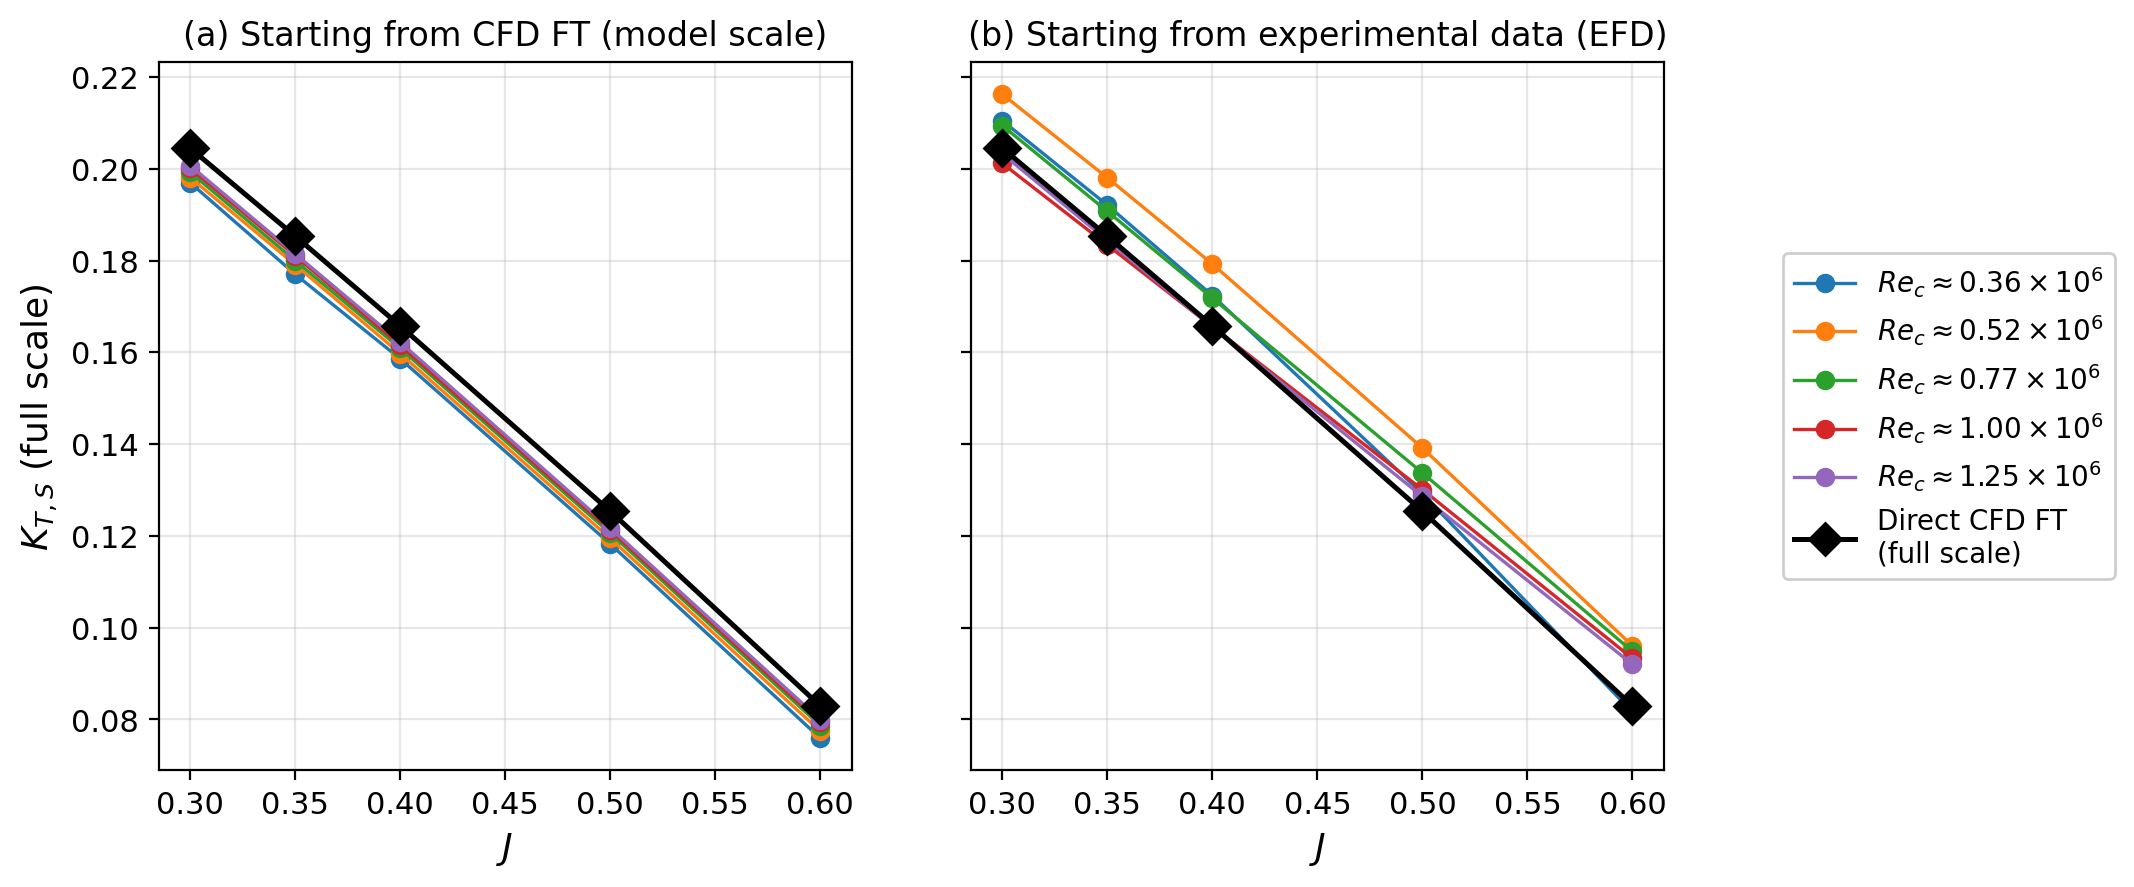
\includegraphics[width=\textwidth]{images/fig_ittc78_vs_cfd_en.png}
    \caption{Predicción de $K_{T,S}$ a escala buque mediante el procedimiento ITTC-78, aplicado a los cinco puntos CFD Fully Turbulent de escala modelo (panel a) y a cada uno de los cinco puntos experimentales de distinto $Re_c$ de modelo (panel b), comparado con el CFD Fully Turbulent resuelto directamente a escala buque (rombos negros).}
    \label{fig:coreana_ittc_vs_cfd}
\end{figure}

Se caracteriza la dispersión de cada columna --el rango de sus cinco predicciones de
escala buque, una por $Re_c$ de ensayo, relativo a la referencia CFD resuelta
directamente a esa escala--:
%
\begin{equation}
\text{dispersión} = 100\,\frac{\max_i K_{T,S}^{i}-\min_i K_{T,S}^{i}}
{K_{T,S}^{\mathrm{CFD}}},
\label{eq:dispersion}
\end{equation}
%
equivalente al rango de los errores de extrapolación de esa columna. El resultado más
relevante de esta comparación no es la media, sino la dispersión de la columna EFD: el
punto de $Re_c = 0.52\times10^6$ --que corresponde casi exactamente
al centro de la ``joroba'' identificada en la Sección~\ref{sec:chichon_antec}, donde el
ensayo registra un $K_T$ anómalamente alto ($0.215$ para $J=0.3$)-- produce por sí
solo un error de extrapolación de $+5.5$ a $+14.5\%$ según el $J$, muy por encima del
resto de los puntos EFD, que en su mayoría predicen razonablemente bien (algunos con
error por debajo del $1\%$). Es decir, la media de la columna EFD ($\sim2.5$--$10.5\%$
según el $J$) esconde un comportamiento muy poco homogéneo: \textbf{el resultado de la
extrapolación depende críticamente de en qué condición de rps se realizó el único
ensayo de túnel disponible}, y si esa condición cae dentro del rango transicional, el
error puede duplicarse o triplicarse respecto de un punto vecino a Reynolds apenas
distinto. Este es precisamente el riesgo práctico señalado en la
Sección~\ref{sec:chichon_antec}: un ensayo de modelo único, realizado sin conocer a
priori si su $Re_c$ cae dentro de la joroba, puede producir una extrapolación ITTC-78
con un error varias veces mayor al que se obtendría con una condición de ensayo apenas
distinta. La brecha se agrava en las condiciones descargadas ($J=0.50$--$0.60$), donde
la propia amplitud de la joroba experimental es mayor (Sección~\ref{sec:coreana_resultados}).

La columna Fully Turbulent, en cambio, es mucho más estable entre puntos para cada $J$
(rango de apenas $2$--$3$ puntos porcentuales dentro de cada columna) pero exhibe un
sesgo sistemático que se profundiza con la descarga del propulsor, de $-2.0\%$ en las
condiciones más cargadas hasta $-10.0\%$ en $J=0.60$, en los cinco puntos y los cinco
$J$ calculados: el ITTC-78, al corregir solo fricción, subestima de forma consistente
el verdadero $K_T$ a $Re_c \approx 1.589\times10^7$. Esta es
la misma conclusión ya obtenida para la B4-60 en la Sección~\ref{sec:helices_ittc78},
ahora confirmada para una segunda geometría y en presencia de un modelo de turbulencia
sin ningún componente transicional.

\subsection{Fracción de presión del efecto de escala del P206}
\label{sec:coreana_fp_correccion}

El sesgo sistemático de la columna Fully Turbulent en la Tabla~\ref{tab:ittc_efd_ft}
es consistente con la conclusión de la Sección~\ref{sec:helices_descomposicion}: el
ITTC-78 ignora la componente de presión del efecto de escala. Para cuantificar esa
componente en el P206 se recurre directamente a la descomposición de fuerzas sobre la
pala, sin inferencias indirectas.

\paragraph{Descomposición directa en dos condiciones de escala buque.} Se dispone de dos
simulaciones completamente turbulentas del mismo propulsor agrandado a $D=6$~m: ambas
corresponden a la misma escala geométrica --con la malla de modelo escalada de manera
uniforme--, y lo que cambia entre ellas es la velocidad de giro, elegida para alcanzar
dos números de Reynolds de escala buque distintos a igual $J$. La primera, a $n=0.80$~rps,
da el $Re_c$ más alto ($Re_c\approx1.589\times10^7$, Tabla~\ref{tab:d6m_resultados}); la
segunda, a $n=0.25$~rps, da un $Re_c$ intermedio entre el de escala modelo y aquel
($Re_c\approx4.97\times10^6$, Tabla~\ref{tab:reint_resultados}), calculado de forma
independiente. Sobre cada uno,
tomando la condición de modelo completamente turbulenta como referencia, la fracción de
presión del efecto de escala se mide directamente como
$f_p=\Delta K_{Tp}/\Delta K_T=\Delta K_{Tp}/(\Delta K_{Tp}+\Delta K_{Tf})$ a partir de la
descomposición de fuerzas de OpenFOAM (Ecuación~\ref{eq:adim_helices}).

\begin{table}[htpb]
\centering
\caption{Resultados de la simulación a $Re_c$ intermedio ($D=6$~m, $n=0.25$~rps,
$Re_c\approx4.97\times10^6$), modelo SST completamente turbulento (OpenFOAM).}
\label{tab:reint_resultados}
\begin{tabular}{cccc}
\hline
$J$ & $K_T$ & $K_Q$ & $\eta_0$ \\
\hline
$0.30$ & $0.202732$ & $0.022043$ & $0.4391$ \\
$0.35$ & $0.183646$ & $0.020550$ & $0.4978$ \\
$0.40$ & $0.164096$ & $0.018977$ & $0.5505$ \\
$0.50$ & $0.123811$ & $0.015548$ & $0.6337$ \\
\hline
\end{tabular}
\end{table}

\begin{table}[htpb]
\centering
\caption{Fracción de presión $f_p = \Delta K_{Tp}/\Delta K_T$ obtenida por
descomposición directa de fuerzas (FT vs.\ FT) para las dos condiciones de escala buque
($Re_c\approx1.589\times10^7$ y $4.97\times10^6$), en función de $J$.}
\label{tab:fp_directo}
\begin{tabular}{ccc}
\hline
$J$ & $f_p$ ($Re_c\approx1.589\times10^7$) & $f_p$ ($Re_c\approx4.97\times10^6$) \\
\hline
$0.30$ & $0.931$ & $0.928$ \\
$0.35$ & $0.929$ & $0.927$ \\
$0.40$ & $0.923$ & $0.920$ \\
$0.50$ & $0.914$ & $0.915$ \\
$0.60$ & $0.898$ & $0.904$ \\
\hline
\end{tabular}
\end{table}

La descomposición directa (Tabla~\ref{tab:fp_directo}) arroja $f_p$ entre $0.90$ y $0.93$, decreciente de forma
monótona con $J$, y prácticamente insensible a la escala: los dos puntos difieren en
menos de $0.01$ en todos los $J$, pese a diferir en un factor $3.2$ en la velocidad de
giro. Es también insensible a cuál de los cinco $Re_c$ de modelo se tome como base de la
comparación (dispersión inferior a $0.01$ en todo $J$), de modo que el valor es una
propiedad del salto de escala y no del par particular de puntos de operación elegido. La
única dependencia robusta es la disminución de $f_p$ con el coeficiente de avance $J$: la
fracción de presión del efecto de escala es mayor en condiciones cargadas. En síntesis,
para el P206 el efecto de escala sobre $K_T$ es de origen de presión en un $90$--$92\%$,
de modo que la fricción --lo único que corrige el ITTC-78-- aporta apenas la fracción
restante.

\paragraph{Comparación con otras geometrías.} Este valor se ubica muy por encima del de
las hélices convencionales de área expandida moderada y muy cerca del de la hélice
geométricamente más parecida al P206. Por un lado, la B4-60 ($A_E/A_0=0.60$, sin skew),
analizada en la Sección~\ref{sec:helices_escala}, presenta $f_p\approx0.69$--$0.77$; un
valor análogo se obtiene para la VP1304 convencional ($A_E/A_0=0.779$) a partir de las
cifras de \citet{gallotti2026}. Por otro lado, el P1727 del mismo trabajo --con $Z=4$,
$A_E/A_0=0.444$ y $c/D_{0.7R}=0.236$, prácticamente idénticos a los del P206
($A_E/A_0=0.431$, $c/D_{0.7R}=0.234$)-- arroja, por descomposición directa de fuerzas,
$f_p\approx0.88$ en el rango de carga de interés, también decreciente con $J$. Queda así
un rango físicamente ordenado por el área expandida: las hélices convencionales de área
moderada (B4-60, VP1304) en $f_p\approx0.70$--$0.77$, y las de área reducida (P206 y
P1727) en la banda alta, $f_p\approx0.88$--$0.92$.

El acuerdo entre el P206 y el P1727 es notable porque el P1727 es una geometría de punta
rakeada (\emph{tip-raked}), mecanismo que el P206 no comparte y que a escala buque agrega
una contribución de presión adicional en la región de punta
\citep{Baltazar2021,gallotti2026}. Cabría esperar, por ello, que su fracción sobrepasara
la del P206; sin embargo, ambas caen prácticamente juntas ($0.88$ frente a
$0.90$--$0.92$). Que la similitud en área expandida y cuerda relativa baste para explicar
fracciones tan próximas, pese a la diferencia de rake, indica que el área expandida
reducida --y no el detalle de la punta-- es el factor que gobierna la elevada fracción de
presión de estas hélices. La coincidencia sirve, además, como respaldo externo de
geometría casi idéntica al valor propio del P206 medido aquí.

\subsection{Implicaciones para el diseño de hélices pequeñas y modelos de disco
actuador}
\label{sec:coreana_implicaciones}

Los dos mecanismos caracterizados en este capítulo --el efecto de escala en régimen turbulento y la transición laminar-turbulenta a escala de modelo-- comparten
el mismo punto ciego del procedimiento ITTC-78, que supone que la totalidad del efecto de
escala es friccional. Ambos, sin embargo, arrastran una contribución de presión que ese
procedimiento no representa: para el primero, un $f_p\approx0.90$--$0.92$ implica que una
corrección puramente friccional, por bien calibrada que esté, no puede por construcción dar
cuenta de más del $8$--$10\%$ del efecto real sobre $K_T$; para el segundo, la
descomposición directa muestra que el desfasaje del modelo transicional respecto del
completamente turbulento es mayoritariamente de presión (del orden del $90\%$), y se
manifiesta también en el par.

Esta limitación tiene una consecuencia directa sobre una clase de aplicaciones cada vez más
frecuente: los modelos de disco actuador empleados para representar el propulsor en
simulaciones de autopropulsión o de interacción casco-hélice. Estos modelos toman como
entrada una curva $K_T$-$K_Q$-$J$ --habitualmente la del ensayo de aguas abiertas a escala
de modelo, o su extrapolación ITTC-78-- y devuelven el empuje y el par distribuidos sobre el
disco. Si el propulsor real opera en régimen transicional, como ocurre en ciertas hélices de
bajo número de Reynolds y en los modelos de ensayo, ninguna curva construida bajo la hipótesis completamente
turbulenta lo representa fielmente, y el disco actuador devolverá empuje y par sesgados sin
ningún indicador interno de la inconsistencia. El sesgo no es despreciable: la
Sección~\ref{sec:coreana_resultados} muestra amplitudes de la joroba de hasta el $16\%$ en
$K_T$, y la Sección~\ref{sec:coreana_ittc_efd_ft} una subestimación sistemática de la extrapolación
ITTC-78 de hasta el $8.5\%$. Para las hélices cuyo número de Reynolds de operación real cae dentro del rango
transicional --como las de vehículos submarinos autónomos y operados remotamente (AUV y
ROV) \citep{pawar2019relevance}--, esto sugiere que la caracterización del régimen
transicional no es un refinamiento académico sino una condición para predecir
correctamente las prestaciones a escala real.

\subsection{Conclusiones parciales}

En el propulsor P206 --de área expandida reducida-- la capa límite a escala
de modelo opera en régimen transicional, y el modelo SST completamente turbulento
--poco sensible a $Re_c$, con un crecimiento monótono leve de apenas $2$ a $6\%$ según
la carga-- no alcanza a reproducir el comportamiento experimental
(Sección~\ref{sec:coreana_resultados}). Los ensayos muestran una joroba transicional:
coeficientes muy superiores a la predicción completamente turbulenta a $Re_c$ bajo,
con una amplitud que crece al descargar el propulsor, del $7.1\%$ a $J=0.30$ al
$16.3\%$ a $J=0.60$; la aproximación entre EFD y SST a medida que $Re_c$ crece es
prácticamente completa a $J\leq0.40$ dentro del rango ensayado, pero a $J=0.50$--$0.60$
persiste una brecha de $5$ a $24\%$ incluso en el mayor $Re_c$ disponible. El modelo
SST-LM captura el mecanismo, pero con fidelidad variable --según el $J$ y el nivel de
$Tu$ subestima o incluso sobrepasa la amplitud medida-- y, sobre todo, ningún valor
único de intensidad turbulenta reproduce la forma de la curva en todo el rango: el
$Tu$ que mejor ajusta cambia de una condición de operación a otra, lo que impide
tratarlo como una propiedad transferible del modelo.

La joroba tiene origen predominantemente de presión. La descomposición directa de las
fuerzas SST-LM muestra que el desfasaje respecto del caso completamente turbulento
proviene en su mayor parte de la presión --del orden del $90\%$--, con la fricción
aportando la fracción menor restante; y el par lo confirma: \emph{aumenta} levemente con
el SST-LM, cuando la fricción, que contribuye positivamente al par, solo podría reducirlo
(Sección~\ref{sec:coreana_resultados}). El diagnóstico seccional
(Sección~\ref{sec:coreana_diagnostico}) localiza el efecto de la transición sobre la
fricción --un frente de transición dependiente de $Tu$ y una tensión de corte
marcadamente más radial, cuya fracción radial pasa de $0.19$ en el caso completamente
turbulento a $0.40$--$0.43$ en el SST-LM-- pero muestra que el cambio de presión no
ocurre en el pico de succión (insensible al modelo, por debajo del $3.1\%$): se trata
de una redistribución de carga a lo largo de la envergadura, consistente con el
mecanismo inferido de los ``paint tests''. La transición se manifiesta así de forma
local y nítida en el campo de fricción, mientras que su efecto dominante sobre el
empuje de presión integrado no está localizado.

La calibración de $Tu$ resulta robusta entre solvers --OpenFOAM y StarCCM+
(Sección~\ref{sec:coreana_solvers})-- y consistente con la validación a $D=6$~m
(Sección~\ref{sec:coreana_d6m}). Trasladado a la extrapolación, el procedimiento
ITTC-78, al suponer un efecto de escala puramente friccional, subestima de forma
sistemática la corrección EFD$\rightarrow$buque hasta en un $8.5\%$
(Sección~\ref{sec:coreana_ittc_efd_ft}). La descomposición directa fija la fracción de
presión del efecto de escala del P206 en $f_p\approx0.90$--$0.92$
(Sección~\ref{sec:coreana_fp_correccion}), de modo que una corrección friccional no
puede dar cuenta de más del $8$--$10\%$ del efecto real; el P1727, hélice de área
reducida geométricamente afín, confirma esa banda con $f_p\approx0.88$, muy por encima
del $0.70$--$0.77$ de las hélices convencionales de área moderada.

En conjunto, ambos mecanismos comprometen la fidelidad de las curvas de aguas abiertas
que alimentan los modelos de disco actuador: construidas bajo la hipótesis
completamente turbulenta o extrapoladas con el ITTC-78, sesgan el empuje y el par de
un propulsor que opera en régimen transicional sin ningún indicador interno de la
inconsistencia (Sección~\ref{sec:coreana_implicaciones}). Para las hélices cuyo Reynolds de
operación real cae en el rango transicional --como las de vehículos submarinos autónomos
y operados remotamente (AUV y ROV)--, caracterizar el régimen transicional deja de ser un
refinamiento académico para volverse una condición de la predicción correcta de
prestaciones a escala real.
\chapter{Conclusiones generales} \label{cap:conclusiones_generales}

El ensayo a escala reducida arrastra una limitación conocida desde los orígenes
de la disciplina: la imposibilidad de satisfacer simultáneamente la semejanza de
todos los números adimensionales que gobiernan el flujo. En la resistencia al
avance, un modelo ensayado en el mismo fluido no puede igualar a la vez el número
de Froude y el de Reynolds del buque: al reducir la escala manteniendo el mismo
fluido y la misma gravedad, conservar el número de Froude obliga a operar a un número
de Reynolds mucho menor que el del buque. En la propulsión, la
misma tensión reaparece entre $Re$ y el coeficiente de avance $J$. Esta semejanza
dinámica parcial es la que introduce los efectos de escala, y su corrección por
vías indirectas constituye el punto de partida de la disciplina, muy anterior a
esta tesis.

Sobre esa dificultad se construyó, mucho antes del CFD, un conjunto de métodos
aproximados. La estrategia fundacional de Froude, respetar la semejanza de Froude
y corregir analíticamente la componente viscosa, dio lugar al factor de forma de
Hughes, al método de extrapolación de Prohaska, a la línea de correlación ITTC-57
y al procedimiento ITTC-78 para hélices, junto con diversas correlaciones
empíricas de corrección de escala. Cada uno de estos métodos resuelve una parte
del problema y arrastra sus limitaciones, porque la corrección viscosa es una
aproximación de un efecto que no puede medirse directamente a escala de modelo. La
línea friccional ITTC no es, en ese sentido, la causa de las dificultades sino una
de las herramientas de ese marco aproximado; su insuficiencia, cuando aparece, es un
síntoma de la aproximación subyacente y no su raíz.

El CFD modifica este panorama, porque permite eludir la limitación de la
semejanza: una simulación puede resolverse directamente al Reynolds de escala
buque, o recurrir a esquemas de escalamiento viscoso, sin la restricción que ata
al ensayo físico. Esa misma virtud, sin embargo, trae aparejada una complicación
que comparte con el ensayo a escala de buque: la ausencia de datos
experimentales con los cuales contrastar el resultado a esa escala. De ahí que el
trabajo se apoye en una combinación deliberada de EFD y CFD, en la que el ensayo
valida la herramienta numérica en el régimen accesible y el CFD, una vez validado,
extiende el análisis hasta la escala buque y descompone las fuerzas en sus
componentes de fricción y de presión, algo fuera del alcance de la medición
integral. Sobre esa base, la tesis contribuye por dos vías complementarias de la
cadena propulsiva: la resistencia al avance, a través del factor de forma $(1+k)$,
y la propulsión, a través del comportamiento de la hélice en aguas abiertas.

\section{Síntesis del Eje 1: resistencia al avance en cascos de baja esbeltez}

El primer eje abordó un tipo de buque escasamente estudiado en la literatura de
hidrodinámica naval: los pesqueros de baja esbeltez ($L/B < 4$), cuyos efectos de
escala en resistencia al avance no habían sido caracterizados con la profundidad
con que sí lo fueron los buques mercantes convencionales. El estudio experimental
del pesquero \textit{P1} (escala 1:20, tres calados) y del casco de referencia
\textit{KCS} (escala 1:79) permitió construir una base de datos de resistencia con
incertidumbres compatibles con las recomendaciones de la ITTC, cuantificadas tanto
por combinación cuadrática (RSS) como mediante el ajuste ponderado de York sobre el
diagrama de Prohaska. Esa base reveló ya una primera asimetría: mientras el
\textit{KCS} satisface con fidelidad los supuestos del método de Prohaska, con sus
puntos alineados sobre la recta teórica y un valor $(1+k) = 1{.}052$ de
incertidumbre relativa $\pm 2{.}3\%$, el \textit{P1} exhibe una curvatura
sistemática a bajos números de Froude y una incertidumbre del ajuste mucho mayor
($8$--$11\%$), señal de que los métodos clásicos se cumplen con menor holgura en un
casco de baja esbeltez.

El aporte central de este eje surgió al extender el análisis a escala buque
mediante CFD en configuración de doble cuerpo (DB). A diferencia del \textit{KCS},
cuyo factor de forma se estabiliza al aumentar el número de Reynolds tal como
predice la teoría clásica, el $(1+k)$ del \textit{P1} crece de manera continua y no
asintótica hasta la escala 1:1. La diferencia entre bajo y alto $Re$ alcanza
aproximadamente un $40\%$ (frente a cerca del $8\%$ en el \textit{KCS}), y el valor
de escala buque $(1+k) \approx 1{.}72$ ($k_S \approx 0{.}72$) resulta casi un
$50\%$ superior al del \textit{KCS}. Un efecto de escala de esta magnitud sobre el
factor de forma es sustancialmente mayor que el observado en los cascos de
referencia caracterizados en el marco del comité de resistencia de la ITTC, y no
tiene precedente documentado para un casco desnudo. Este comportamiento no es una
singularidad del \textit{P1}: los tres pesqueros analizados (\textit{P1},
\textit{P2} y \textit{P3}, con $L/B$ entre $2{.}85$ y $3{.}53$) reproducen la misma
tendencia creciente, lo que la establece como un rasgo estructural de los cascos
con $L/B < 4$.

El mecanismo físico responsable se aisló mediante la descomposición de la
resistencia viscosa que solo el CFD DB hace posible. El crecimiento sostenido de
$(1+k)$ se debe a la persistencia de la componente de presión viscosa $C_{PV}$,
originada en un déficit de recuperación de presión en la popa llena del casco y en
estructuras vorticosas longitudinales desprendidas de la quilla y el pantoque, que
se mantienen prácticamente invariantes con la escala. Al disminuir $C_{F0}$ con el
Reynolds sin que $C_{PV}$ lo acompañe, el cociente que define el factor de forma no
puede estabilizarse. Los análisis complementarios permitieron descartar
explicaciones alternativas: la proa bulbo modifica $(1+k)$ pero no explica ni la
curvatura del diagrama ni la ausencia de asíntota, que persisten en la variante sin
bulbo; la popa espejo sumergida, tratada con el método de dos factores de forma
$2k$, aporta $k_{tr} = 0{.}025$, apenas un $5\%$ del efecto de escala total
($k_S - k_M = 0{.}522$); y la sustitución de la línea ITTC-57 por líneas de fricción
numéricas atenúa la dependencia con $Re$ pero no la elimina. El efecto dominante es,
por lo tanto, la evolución de $C_{PV}$ gobernada por la geometría de baja esbeltez.

Como consecuencia directa, las correlaciones empíricas navales de corrección de
escala fallan en este régimen: la fórmula de \citet{gomezgarcia}, por ejemplo,
subestima el efecto de escala del \textit{P1} en más de un orden de magnitud,
porque fue calibrada para cascos con $L/B$ entre $6{.}98$ y $9{.}07$, muy lejos del
dominio de los pesqueros. En cambio, las correlaciones aerodinámicas de factor de
forma para cuerpos de revolución de baja esbeltez (\citealp{raymer2019aircraft,
roskam1987airplane}) reproducen con notable fidelidad los valores de CFD DB de los
tres pesqueros, ubicándolos en una región coherente con su $L/B$. Este hallazgo
abre la posibilidad de desarrollar una formulación empírica específica de $(1+k)$
en función de $L/B$ para cascos de baja esbeltez, que hoy carecen de una
herramienta de estimación confiable.

\section{Síntesis del Eje 2: efectos de escala en la hélice}

El segundo eje trasladó la misma dificultad de fondo, la imposibilidad de conservar
simultáneamente $Re$ y $J$ en el ensayo, al comportamiento de la hélice en aguas
abiertas, caracterizando dos mecanismos físicamente independientes de efecto de
escala. Ambos comparten el punto ciego del procedimiento ITTC-78: la suposición de
que la corrección de modelo a buque es puramente friccional ($\Delta K_{Tp} = 0$).

El primero es el efecto de escala entre condiciones completamente turbulentas (de
modelo a buque, ambas en régimen turbulento pleno), estudiado sobre la hélice
Wageningen B4-60 mediante un barrido de diámetros de $D = 0{.}14$ a $8{.}0$~m. Al
aumentar el Reynolds, el empuje crece ($\Delta K_T = +4{.}7\%$) y el par disminuye
($-4{.}1\%$), con una ganancia neta de eficiencia en aguas abiertas de $+9{.}1\%$.
La descomposición directa de fuerzas mostró que ese aumento de empuje está dominado
por la presión: la fracción $\Delta K_{Tp}/\Delta K_T$ se estabiliza en torno al
$76$--$77\%$, de modo que apenas una cuarta parte proviene de la reducción de
fricción. El análisis del campo de presión localizó esta redistribución sobre el
lado de succión de la mitad externa de la pala, intensificándose hacia la punta. El
procedimiento ITTC-78, al corregir solo fricción, predice una ganancia de eficiencia
de apenas $+1{.}1\%$ frente al $+9{.}1\%$ del CFD, una diferencia de unos $8$ puntos
porcentuales que corresponde íntegramente a la componente de presión ignorada.

El segundo mecanismo es la transición laminar-turbulenta sobre las palas a escala de
modelo, estudiada sobre el propulsor \textit{P206}, ensayado en túnel de cavitación
a cinco números de Reynolds de cuerda. Los ensayos revelan una joroba transicional
en $K_T$ y $K_Q$ cuya amplitud, medida como la diferencia entre los coeficientes
experimentales y la predicción completamente turbulenta, crece al descargar el
propulsor, desde un $7{.}1\%$ a $J = 0{.}30$ hasta un $16{.}3\%$ a $J = 0{.}60$. El
modelo completamente turbulento no reproduce este comportamiento en ningún caso, y
el modelo de transición ($\gamma$-$\widetilde{Re}_{\theta t}$), verificado en dos
solvers independientes (OpenFOAM y StarCCM+), lo captura solo parcialmente: ningún
valor único de intensidad turbulenta reproduce la forma de la curva en todo el rango
de operación, lo que impide tratar ese parámetro como una propiedad transferible.

No fue posible reproducir con exactitud los valores experimentales de $K_T$ y $K_Q$ en el régimen
transicional con ningún valor de intensidad turbulenta ni con ninguno de los dos
solvers empleados. Sin embargo, la descomposición directa de las fuerzas mostró que
el desplazamiento de la curva completamente turbulenta hacia los valores
experimentales es de origen mayoritariamente de presión --del orden del $90\%$--: la
componente friccional aporta la fracción menor, y el par incluso aumenta levemente
con el modelo de transición, cuando una reducción puramente friccional lo disminuiría.
La limitación remanente no es, entonces, la de identificar el mecanismo, sino la de que
ningún nivel único de intensidad turbulenta reproduce la joroba experimental en todo el
rango de operación. Al propagar esta física a
través del ITTC-78 se constató un doble problema: un sesgo sistemático de
subestimación de hasta el $8{.}5\%$, y, más grave, que el resultado de la
extrapolación depende críticamente de en qué velocidad de giro se realizó el único
ensayo de túnel disponible, de modo que si esa condición cae dentro de la joroba el
error puede duplicarse o triplicarse respecto de un punto vecino a Reynolds apenas
distinto.

La fracción de presión del efecto de escala completamente turbulento del
\textit{P206} se midió de forma directa, como el cociente $\Delta K_{Tp}/\Delta K_T$
obtenido al descomponer las fuerzas sobre la pala en sus componentes de presión y
fricción entre la condición de modelo y la de escala buque, ambas completamente
turbulentas, resultando $f_p \approx 0{.}90$--$0{.}92$. El valor es mayor que el de la
B4-60 ($0{.}70$--$0{.}77$) y prácticamente coincide con el de la hélice geométricamente
más parecida al \textit{P206} (el P1727, $\approx 0{.}88$), lo que sugiere que la
elevada fracción de presión está gobernada por el área expandida reducida; establecer
esa dependencia geométrica con generalidad requiere el mapeo sistemático que se plantea
como trabajo futuro.

A diferencia del eje de resistencia, donde la evidencia acumulada sobre tres cascos
permitió proponer una generalización geométrica del comportamiento en función de
$L/B$, el eje propulsivo deja el problema mucho más abierto. Los resultados aquí
obtenidos se apoyan en solo dos hélices estudiadas en detalle, la B4-60 y el
\textit{P206}, y en una tercera tomada como referencia externa de la bibliografía
reciente. La dependencia de la fracción de presión y de la joroba transicional con
los parámetros geométricos de la pala (número de palas, razón de áreas $A_E/A_0$,
skew, distribución de cuerdas) apenas comienza a esbozarse, y su generalización,
análoga a la lograda para el factor de forma con $L/B$, requiere una base de
geometrías considerablemente más amplia. El campo de los efectos de escala en
hélices permanece, en consecuencia, sensiblemente más abierto que el de la
resistencia.

\section{El hilo conductor: la componente de presión del efecto de escala}

Leídos en conjunto, los dos ejes convergen en una misma conclusión física. Frente a
la imposibilidad de la semejanza dinámica completa, los procedimientos vigentes
corrigen la componente viscosa suponiendo que el efecto de escala es esencialmente
friccional. Esta tesis muestra, en dos contextos independientes de la cadena
propulsiva, que ese supuesto es incompleto: en la resistencia, la incapacidad de
$(1+k)$ para estabilizarse con la escala se explica por una componente de presión
viscosa que persiste con el Reynolds; en la propulsión, el efecto de escala entre
condiciones completamente turbulentas está dominado por la redistribución de presión
sobre la pala, y la joroba transicional apunta, con la cautela ya señalada, en la
misma dirección. En ambos casos, el mecanismo que gobierna el escalado no es el que
los métodos estándar corrigen: la parte friccional captura la fracción menor del
fenómeno y omite la mayor. Haber cuantificado esa componente de presión constituye la
contribución transversal del trabajo.

\section{Impacto sobre la predicción de potencia del buque}

La consecuencia práctica de estos resultados se materializa al estimar la potencia
del \textit{P1} a escala buque. En el eje de resistencia, la comparación entre el
método ITTC estándar (que asume $k_S = k_M$) y un método de doble factor de forma
basado en CFD DB (con $k_M$ y $k_S$ determinados numéricamente en cada escala)
arroja diferencias del $13$ al $17\%$ en la potencia efectiva, gobernadas
directamente por el salto $k_S \gg k_M$ que constituye el resultado central del
primer eje. A modo de referencia, ignorar por completo el factor de forma ($k = 0$)
produce una sobrestimación de solo un $5\%$, lo que evidencia que la fuente de
discrepancia no es el procedimiento en sí, sino la magnitud del efecto de escala del
factor de forma, mucho mayor que el que asumen implícitamente los métodos vigentes.

En el eje propulsivo, la subestimación de la eficiencia en aguas abiertas, de unos
$8$ puntos porcentuales por el efecto de escala completamente turbulento (la
diferencia entre el $+9{.}1\%$ del CFD y el $+1{.}1\%$ del ITTC-78) y de hasta un
$8{.}5\%$ por el sesgo transicional del procedimiento, actúa sobre el otro extremo
del cálculo de potencia, degradando la predicción del rendimiento propulsivo. Dado
que resistencia y propulsión se combinan en la estimación de la potencia instalada,
sus contribuciones no se cancelan sino que se acumulan. Discrepancias del orden del
$15\%$ en potencia son suficientemente significativas desde el punto de vista del
diseño como para justificar su validación mediante pruebas de mar y para
desaconsejar la aplicación acrítica de los procedimientos estándar.

\section{El aporte metodológico: la sinergia EFD-CFD}

El resultado transversal de la tesis, tanto en resistencia como en propulsión, solo
fue posible gracias a la combinación deliberada de experimentación y simulación, en
la que cada herramienta suple las limitaciones de la otra. El CFD permite eludir la
restricción de la semejanza y alcanzar la escala buque, pero, al igual que el ensayo
a escala de buque, carece de un dato experimental con el cual contrastarse a
esa escala; el ensayo físico, a su vez, solo accede al régimen de modelo. La
validación cruzada entre ambos, en el régimen donde el ensayo es posible, no garantiza
por sí sola la exactitud del resultado a escala buque --que permanece sin un dato
experimental que lo confirme--, pero sí respalda las tendencias que la simulación
predice al cambiar de escala: la evolución de las distribuciones de presión, de las
fuerzas y de los regímenes de flujo. Es esto lo que permite comprender qué mecanismos
pueden estar gobernando el comportamiento a escala real.

La experimentación aportó la base validada e imprescindible: curvas de resistencia y
de aguas abiertas con incertidumbre cuantificada, que anclan el análisis en datos
reales. El acuerdo entre los ensayos del LabHiNO y las referencias internacionales,
las mediciones del \textit{KCS} frente a los datos de distintos laboratorios y las de
la B4-60 frente a MARIN, confirmó la calidad de la campaña experimental y habilitó el
uso del canal como fuente confiable de validación.

El CFD, a su vez, aportó lo que el ensayo no puede: por un lado, el acceso a escalas
de Reynolds inalcanzables en un canal de dimensiones finitas, que permitió observar
la evolución de $(1+k)$ y de los coeficientes de la hélice hasta la escala buque; por
otro, la descomposición de las fuerzas en sus componentes de fricción y de presión,
sin la cual el mecanismo físico del efecto de escala habría permanecido oculto tras
una fuerza integral. Fue esta descomposición la que reveló el papel dominante de
$C_{PV}$ en el factor de forma y la que permitió cuantificar la fracción de presión
$f_p$ de la hélice.

La sinergia es, además, específica de cada problema. En el factor de forma, la
combinación EFD-CFD hizo posible el método de doble cuerpo, que determina $k_M$ y
$k_S$ de forma independiente y resulta más robusto que el método de Prohaska
precisamente en los cascos donde este último se vuelve menos confiable. En
propulsión, la combinación permitió discriminar el efecto de escala completamente
turbulento del mecanismo transicional, que un modelo totalmente turbulento no puede
capturar y que solo el CFD de transición, anclado en datos de túnel, reproduce.

\section{Aportes principales}

Los aportes originales de esta tesis pueden resumirse en los siguientes puntos:

\begin{itemize}
    \item Se caracterizó en profundidad, por primera vez sobre datos propios y para
    tres cascos distintos, el efecto de escala del factor de forma en pesqueros de
    baja esbeltez ($L/B < 4$), un tipo de buque escasamente estudiado, mostrando que
    $(1+k)$ crece de manera continua y no asintótica con el número de Reynolds hasta
    la escala buque, con una magnitud muy superior a la de los cascos de referencia
    caracterizados en el marco del comité de resistencia de la ITTC.

    \item Se identificó a la componente de presión viscosa $C_{PV}$ de la popa como la
    causa física dominante de ese comportamiento, y se cuantificó y descartó, mediante
    los análisis de proa bulbo, popa espejo sumergida ($2k$) y línea de fricción, el
    peso de las causas alternativas.

    \item Se mostró la inaplicabilidad de las correlaciones navales de factor de forma
    a esta clase de cascos y se propuso el uso de correlaciones aerodinámicas de
    cuerpos de revolución en función de $L/B$ como marco más apropiado, abriendo la vía
    a una formulación empírica específica.

    \item Se cuantificó, para la hélice B4-60, que la componente de presión domina el
    efecto de escala completamente turbulento sobre el empuje ($\sim 76$--$77\%$).

    \item Se caracterizó, experimental y numéricamente, el comportamiento del propulsor
    \textit{P206} en régimen transicional, describiendo la joroba en $K_T$ y $K_Q$ y
    poniendo en evidencia el problema que supone extrapolar las prestaciones desde ese
    régimen, donde el resultado depende críticamente del número de Reynolds al que se
    realizó el ensayo.

    \item Se analizó, por separado, el efecto de escala completamente turbulento del
    \textit{P206}, cuantificando su fracción de presión en $f_p \approx 0{.}90$--$0{.}92$
    mediante la descomposición directa de fuerzas, un valor muy superior al de las
    hélices convencionales de área moderada.

    \item Se evaluó el impacto de estos efectos sobre la predicción de potencia,
    mostrando diferencias del orden del $13$--$17\%$ en potencia efectiva por el factor
    de forma y de hasta el $8{.}5\%$ en eficiencia propulsiva por el sesgo del ITTC-78,
    y se propusieron métodos de doble $k$ y correcciones de fricción y presión que los
    incorporan.

    \item Se consolidó una metodología combinada EFD-CFD, validada frente a
    referencias internacionales, capaz de abordar problemas de escala que ni la
    experimentación ni la simulación resuelven por separado.
\end{itemize}

\section{Líneas futuras de investigación}

El trabajo realizado deja abiertas varias direcciones de continuación, con un grado
de madurez distinto en cada eje. En resistencia, la caracterización alcanzada permite
plantear objetivos de consolidación; en propulsión, el campo se encuentra
considerablemente más abierto.

\begin{itemize}
    \item El desarrollo y la calibración de una correlación empírica de $(1+k)$ en
    función de $L/B$ para cascos pesqueros, específicamente en el rango $L/B < 4$, a
    partir de una base ampliada de geometrías, que permita estimar $k_S$ sin recurrir
    a simulaciones CFD a escala buque.

    \item La validación de las predicciones de potencia mediante pruebas de mar sobre
    buques en escala 1:1, dada la magnitud de las discrepancias frente a los métodos estándar.

    \item En el terreno propulsivo, la búsqueda de una generalización del efecto de
    escala y de la fracción de presión en función de la geometría de la pala (número de
    palas, razón de áreas $A_E/A_0$, skew, distribución de cuerdas), a partir de un
    conjunto de hélices mucho más amplio que las estudiadas aquí. Es la contrapartida
    propulsiva de la generalización lograda con $L/B$ para la resistencia, y permanece
    esencialmente pendiente.

    \item La exploración de la introducción deliberada de turbulencia sobre las palas,
    mediante turbuladores o rugosidad controlada, como estrategia para forzar un régimen
    completamente turbulento a escala de modelo y evitar así la joroba transicional
    observada tanto en los ensayos (EFD) como en el modelo de transición (SST-LM). De
    confirmarse, esta vía volvería más predecible el ensayo de aguas abiertas y su extrapolación,
    al ubicar el punto de operación fuera del rango ambiguo.

    \item La determinación de la forma funcional $f_p(Re)$ de la fracción de presión, y
    la incorporación de las correcciones de presión, en resistencia y en propulsión, a
    los procedimientos de predicción de potencia, hacia un esquema de extrapolación que
    no suponga que el efecto de escala es puramente friccional.

    \item La extensión del análisis a la condición autopropulsada completa, que integre
    la interacción casco-hélice y permita evaluar el impacto conjunto de ambos ejes
    sobre el punto de operación real del buque.
\end{itemize}

En conjunto, esta tesis aporta en un terreno poco explorado. En resistencia,
caracteriza el efecto de escala del factor de forma en pesqueros de baja esbeltez y
lo explica por una componente de presión que los métodos estándar no contemplan,
dejando al alcance una generalización geométrica en función de $L/B$. En propulsión,
cuantifica el peso de la presión en el efecto de escala de la hélice y describe la
joroba transicional, abriendo un terreno donde el mapeo del
comportamiento en función de la geometría de la pala queda por delante. En ambos
frentes, la combinación de experimentación y simulación numérica se muestra como la
herramienta adecuada: el ensayo aporta la validación en el régimen accesible, el CFD
el acceso a la escala real y a la física subyacente, y solo su uso conjunto permite
cuantificar la componente de presión del efecto de escala que los procedimientos
vigentes, apoyados en una hipótesis puramente friccional, dejan fuera. El eje de
resistencia queda así caracterizado con una generalización geométrica al alcance;
el de propulsión, con un campo todavía ancho por delante.
\newpage
\bibliographystyle{plainnat}
\bibliography{referencias}

\end{document}